%!TEX ROOT=ctutest.tex


\chapter{Deep Deterministic Policy Gradient}
\label{chapter:ddpg}

In this section I describe the DDPG algorithm, detailing the implementation process and the experiments.

\section{The DDPG Algorithm}

Lillicrap, Hunt et al \cite{cite:DDPG} have taken the ideas underlying the success of Deep Q-Learning and combined them with the deterministic policy gradient. 

The main difference between DQL and DDPG lies in the choice of the actor. In DQL, the actor is not explicitly represented and each action is chosen as the $\text{argmax}_a Q(s,a)$. This approach is feasible only in small action spaces and in larger spaces it would require demanding parameter search during each learning step. In DDPG, the actor is another function approximator that inputs state $s_t$ and outputs action $a_t$, $\mu_\theta(s_t)=a_t$.

\begin{algorithm}[ph!]
  \caption{DDPG algorithm }
  \label{algo:ddpg}
  \begin{algorithmic}
    \STATE Randomly initialize critic network $Q(s, a | \theta^Q)$ and actor
    $\mu(s | \theta^{\mu})$ with weights $\theta^{Q}$ and $\theta^{\mu}$.
    \STATE Initialize target network $Q'$ and $\mu'$ with weights $\theta^{Q'}
    \leftarrow \theta^{Q}$, $\theta^{\mu'} \leftarrow \theta^{\mu}$
    \STATE Initialize replay buffer $R$
    \FOR{episode = 1, M}
      \STATE Initialize a random process $\mathcal{N}$ for action
      exploration
      \STATE Receive initial observation state $s_1$
      \FOR{t = 1, T}
        \STATE Select action $a_t = \mu(s_t | \theta^{\mu}) + \mathcal{N}_t$
        according to the current policy and exploration noise
        \STATE Execute action $a_t$ and observe
        reward $r_t$ and observe new state $s_{t+1}$
        \STATE Store transition $(s_t, a_t,
                r_t, s_{t+1})$ in $R$
        \STATE Sample a random minibatch of $N$ transitions
               $(s_i, a_i,
        r_i, s_{i + 1})$ from $R$
        \STATE Set $ y_i = 
            \begin{cases}
            r_i + \gamma Q'(s_{i + 1}, \mu(s_{i+1})) & \text {for non terminal state} \\
            r_i & \text{for terminal state} \\
            \end{cases} $
        \STATE Update critic by minimizing the loss:
               $L = \frac{1}{N} \sum_i (y_i -
               Q(s_i, a_i | \theta^Q))^2$
        \STATE Update the actor policy using the sampled policy gradient:
        \begin{equation*}
            \nabla_{\theta^{\mu}} J \approx
            \frac{1}{N} \sum_i
               \nabla_{a} Q(s, a | \theta^Q)|_{s = s_i, a = \mu(s_i)}
               \nabla_{\theta^\mu} \mu(s | \theta^\mu)|_{s_i}
         \end{equation*}
        \STATE Update the target networks:
          \begin{equation*}
            \theta^{Q'} \leftarrow \tau \theta^{Q} + (1 - \tau) \theta^{Q'}
          \end{equation*}
          \begin{equation*}
            \theta^{\mu'} \leftarrow \tau \theta^{\mu} +
                (1 - \tau) \theta^{\mu'}
          \end{equation*}
        \ENDFOR
    \ENDFOR
  \end{algorithmic}
\end{algorithm}


The Deep Deterministic Policy Gradient (DDPG, see algorithm \ref{algo:ddpg} at the end of this chapter) has been successfully applied on an array of diverse continuous control tasks including cartpole swingup, 2D legged locomotion or dexterous manipulation. Some of the tasks were also solved directly from visual inputs. However, it has not been used for locomotion in three dimensions.

\section{Implementation}
Following the implementation of the supervised methods, I continued with the Theano library. Making the code work has proved to be quite a challenge due to several important details that slipped the current (at the time of implementation the paper was just submitted to the ICLR 2016 conference) version of the DDPG paper.

\subsection{DPG Simplification}
The deterministic policy gradient, as presented in both DPG and DDPG papers is in the form of
\[
\nabla_\theta J(\mu_\theta)= \mathbb{E}_{s\sim\rho^\mu}[\nabla_\theta \mu_\theta(s) \nabla_aQ^\mu(s,a)]
\]
To add confusion, in the DPG paper the expression is presented in reverse order ($\nabla_\theta J(\mu_\theta)= \mathbb{E}_{s\sim\rho^\mu}[\nabla_aQ^\mu(s,a)\nabla_\theta \mu_\theta(s)]$).

The equation consists of two terms:
\begin{itemize}
\item $\nabla_aQ^\mu(s,a)$: this is a row vector containing the expression 
\[ \nabla_aQ^\mu(s,a)=\left[ \dfrac{\partial Q}{\partial a_1}, \dots , \dfrac{\partial Q}{\partial a_n} \right] \]

\item $\nabla_\theta \mu_\theta(s)$:  this is a matrix of size $n \times l$\footnote{
$m=$ size of the state feature vector, 
$n=$ size of the action, 
$l=$ number of actor parameters
}
\[
  \nabla_\theta \mu_\theta(s)=
  \left[ {\begin{array}{ccc}
   \dfrac{\partial a_1}{\partial \theta_1} & \dots & \dfrac{\partial a_1}{\partial \theta_l}\\
\vdots & \ddots & \vdots \\
\dfrac{\partial a_n}{\partial \theta_1} & \dots & \dfrac{\partial a_n}{\partial \theta_l}

      \end{array} } \right]
\]
\end{itemize}
When comparing the dimensions, the order became clear ($1 \times n \cdot n \times l = 1 \times l$). What's more important, after multiplying these terms we arrive at the following expression

\[ 
\nabla_aQ^\mu(s,a)\nabla_\theta \mu_\theta(s)=\left[ \sum_{i=1}^n \dfrac{\partial Q}{\partial a_i}\dfrac{\partial a_i}{\partial \theta_1}\quad \dots \quad \sum_{i=1}^n \dfrac{\partial Q}{\partial a_i}\dfrac{\partial a_i}{\partial \theta_l}\right]
\]

After examining the equations, it became clear that each term  represents the multidimensional chain rule of 
\[
\sum_{i=1}^n \dfrac{\partial Q}{\partial a_i}\dfrac{\partial a_i}{\partial \theta_j} = \dfrac{\partial Q}{\partial \theta_j}
\]
This simplifies the original expression as
\begin{equation}
\nabla_{\theta^{\mu}} J=\nabla_aQ^\mu(s,a)\nabla_\theta \mu_\theta(s)=\nabla_{\theta^\mu} Q(s, \mu (s))
\end{equation}

This rewritten formula is very intuitive, since it says that following the gradient of the reward function with respect to actor's parameters is the same as following the gradient of the critic with respect to the actor's parameters. We are trying to maximize the critic's output!

While in the end I found the equations mentioned in the DPG paper, they are not represented as the final result for some reason.

This small change (basically just a rewrite) has shed light for me on the problematic and allowed the implementation of a much simpler and cleaner (and faster) version of the DDPG algorithm.


\subsection{Critic updates}
Another fact missing from the DDPG paper was the complete computation of the $y$ term used for learning the critic.

In the paper, the $y$-term is computed as $y_i=r_i + \gamma Q'(s_{i + 1}, \mu(s_{i+1}))$. This unfortunately doesn't tell us what to do with the terminating state. I followed the same formula used in DQN, where it is necessary to ground the critic in the terminating state as $y_i=r_i$.
\medskip

When conducting experiments, I tried several different settings and it turned out that even when the terminating state was not bounded, the algorithm was able to converge on simpler tasks. This is most probably due to the fact that, compared to DQN, DDPG doesn't care about the absolute values of the critic and only uses it's gradient.

In the end I opted for the bounded version on all of the experiments.

\subsection{Adam}
In my experience, the difference between using SGD and its variants (AdaGrad, AdaMax, RMSProp, Adam) is usually a few percent points in the loss function value after training. This is why I skipped the implementation of Adam (using simple SGD) and focused on different parts of the code.

This has turned out to be a crucial mistake, because the algorithm without Adam was unable to converge. It is unclear if the authors knew about this issue, since they didn't mention it in the paper. See \ref{fig:adam-sgd} for the comparison.

\begin{figure}[htbp]
\input{plots/ddpg/adam_sgd.pgf}
\caption{Comparison of Adam and SGD algorithms on the swingup task. Actor=\{50,50\}, Critic=\{100,100\}}
\centering
\label{fig:adam-sgd}
\end{figure}

\section{Exploration vs Exploitation}

Exploration vs exploitation is a dilemma that a RL agent faces when optimizing for some loss function that is a function of the environment. 

At any given point in time the agent has to choose an action from the action space. The exploitation approach would be to choose the action that he knows will produce the most reward. However it is possible (and often the case) that taking another action will lead to a grater reward down the path.

The exploration in the DDPG paper is done by adding time-correlated noise to the actions. The used noise is generated with Ornstein-Uhlenbeck process. 

\subsection{Ornstein-Uhlenbeck Process}
The Ornstein–Uhlenbeck (OU) process is a stochastic process that, roughly speaking, describes the velocity of a massive Brownian particle under the influence of friction. The process is stationary, Gaussian, and Markovian, and it is the only nontrivial process that satisfies these three conditions, up to allowing linear transformations of the space and time variables. The process can be considered to be a modification of the random walk in continuous time, or Wiener process, in which the properties of the process have been changed so that there is a tendency of the walk to move back towards a central location, with a greater attraction when the process is further away from the center. \cite{cite:wiki-ou}

An OU process satisfies the following stochastic differential equation
\begin{equation}
\text{d}x_t=\theta(\mu-x_t)\text{d}t+\sigma \text{d}W_t
\end{equation}
where $\theta>0 , \mu , \sigma>0$ are the parameters and $W_t$ denotes the Wiener process. The incremental solution can be then written as
\begin{equation}
x_t=x_0 e^{-\theta t}+\mu(1-e^{-\theta t})+\dfrac{\sigma}{\sqrt{2\theta}}e^{-\theta t}W_{e^{2\theta t}-1}
\end{equation}
This incremental solution is used in the final implementation. See \ref{plot:ou} for example runs.

The noise is an instrumental part of the DDPG algorithm and without it, there is a little chance the model will find any good solutions and most likely gets stuck in a local extreme. See \ref{plot:ou-compare} for comparisons with and without using noise.

\begin{figure}[h!]
%% Creator: Matplotlib, PGF backend
%%
%% To include the figure in your LaTeX document, write
%%   \input{<filename>.pgf}
%%
%% Make sure the required packages are loaded in your preamble
%%   \usepackage{pgf}
%%
%% Figures using additional raster images can only be included by \input if
%% they are in the same directory as the main LaTeX file. For loading figures
%% from other directories you can use the `import` package
%%   \usepackage{import}
%% and then include the figures with
%%   \import{<path to file>}{<filename>.pgf}
%%
%% Matplotlib used the following preamble
%%   \usepackage[utf8x]{inputenc}
%%   \usepackage[T1]{fontenc}
%%
\begingroup%
\makeatletter%
\begin{pgfpicture}%
\pgfpathrectangle{\pgfpointorigin}{\pgfqpoint{5.022831in}{2.009132in}}%
\pgfusepath{use as bounding box, clip}%
\begin{pgfscope}%
\pgfsetbuttcap%
\pgfsetmiterjoin%
\definecolor{currentfill}{rgb}{1.000000,1.000000,1.000000}%
\pgfsetfillcolor{currentfill}%
\pgfsetlinewidth{0.000000pt}%
\definecolor{currentstroke}{rgb}{1.000000,1.000000,1.000000}%
\pgfsetstrokecolor{currentstroke}%
\pgfsetdash{}{0pt}%
\pgfpathmoveto{\pgfqpoint{0.000000in}{0.000000in}}%
\pgfpathlineto{\pgfqpoint{5.022831in}{0.000000in}}%
\pgfpathlineto{\pgfqpoint{5.022831in}{2.009132in}}%
\pgfpathlineto{\pgfqpoint{0.000000in}{2.009132in}}%
\pgfpathclose%
\pgfusepath{fill}%
\end{pgfscope}%
\begin{pgfscope}%
\pgfsetbuttcap%
\pgfsetmiterjoin%
\definecolor{currentfill}{rgb}{1.000000,1.000000,1.000000}%
\pgfsetfillcolor{currentfill}%
\pgfsetlinewidth{0.000000pt}%
\definecolor{currentstroke}{rgb}{0.000000,0.000000,0.000000}%
\pgfsetstrokecolor{currentstroke}%
\pgfsetstrokeopacity{0.000000}%
\pgfsetdash{}{0pt}%
\pgfpathmoveto{\pgfqpoint{0.607535in}{0.495779in}}%
\pgfpathlineto{\pgfqpoint{4.754774in}{0.495779in}}%
\pgfpathlineto{\pgfqpoint{4.754774in}{1.810070in}}%
\pgfpathlineto{\pgfqpoint{0.607535in}{1.810070in}}%
\pgfpathclose%
\pgfusepath{fill}%
\end{pgfscope}%
\begin{pgfscope}%
\pgfpathrectangle{\pgfqpoint{0.607535in}{0.495779in}}{\pgfqpoint{4.147239in}{1.314291in}} %
\pgfusepath{clip}%
\pgfsetrectcap%
\pgfsetroundjoin%
\pgfsetlinewidth{0.501875pt}%
\definecolor{currentstroke}{rgb}{0.000000,0.000000,1.000000}%
\pgfsetstrokecolor{currentstroke}%
\pgfsetdash{}{0pt}%
\pgfpathmoveto{\pgfqpoint{0.607336in}{0.672753in}}%
\pgfpathlineto{\pgfqpoint{0.616224in}{0.684585in}}%
\pgfpathlineto{\pgfqpoint{0.639581in}{0.684487in}}%
\pgfpathlineto{\pgfqpoint{0.643038in}{0.708881in}}%
\pgfpathlineto{\pgfqpoint{0.648342in}{0.805436in}}%
\pgfpathlineto{\pgfqpoint{0.655241in}{0.793123in}}%
\pgfpathlineto{\pgfqpoint{0.661830in}{0.797659in}}%
\pgfpathlineto{\pgfqpoint{0.668980in}{0.807133in}}%
\pgfpathlineto{\pgfqpoint{0.675111in}{0.810921in}}%
\pgfpathlineto{\pgfqpoint{0.695007in}{0.816315in}}%
\pgfpathlineto{\pgfqpoint{0.702614in}{0.812948in}}%
\pgfpathlineto{\pgfqpoint{0.710081in}{0.818478in}}%
\pgfpathlineto{\pgfqpoint{0.722835in}{0.824874in}}%
\pgfpathlineto{\pgfqpoint{0.729337in}{0.832737in}}%
\pgfpathlineto{\pgfqpoint{0.736199in}{0.819710in}}%
\pgfpathlineto{\pgfqpoint{0.742998in}{0.820271in}}%
\pgfpathlineto{\pgfqpoint{0.749709in}{0.798709in}}%
\pgfpathlineto{\pgfqpoint{0.757006in}{0.794201in}}%
\pgfpathlineto{\pgfqpoint{0.763398in}{0.797754in}}%
\pgfpathlineto{\pgfqpoint{0.770571in}{0.804652in}}%
\pgfpathlineto{\pgfqpoint{0.777893in}{0.799149in}}%
\pgfpathlineto{\pgfqpoint{0.785529in}{0.801118in}}%
\pgfpathlineto{\pgfqpoint{0.792926in}{0.798938in}}%
\pgfpathlineto{\pgfqpoint{0.801015in}{0.812080in}}%
\pgfpathlineto{\pgfqpoint{0.810033in}{0.807969in}}%
\pgfpathlineto{\pgfqpoint{0.833287in}{1.016893in}}%
\pgfpathlineto{\pgfqpoint{0.862081in}{1.229399in}}%
\pgfpathlineto{\pgfqpoint{0.891926in}{1.196091in}}%
\pgfpathlineto{\pgfqpoint{0.921771in}{1.249411in}}%
\pgfpathlineto{\pgfqpoint{0.951616in}{1.219034in}}%
\pgfpathlineto{\pgfqpoint{0.979370in}{1.234135in}}%
\pgfpathlineto{\pgfqpoint{1.009215in}{1.301430in}}%
\pgfpathlineto{\pgfqpoint{1.039060in}{1.196829in}}%
\pgfpathlineto{\pgfqpoint{1.068905in}{1.282097in}}%
\pgfpathlineto{\pgfqpoint{1.098750in}{1.253794in}}%
\pgfpathlineto{\pgfqpoint{1.158441in}{1.306844in}}%
\pgfpathlineto{\pgfqpoint{1.181249in}{0.837763in}}%
\pgfpathlineto{\pgfqpoint{1.204594in}{1.050988in}}%
\pgfpathlineto{\pgfqpoint{1.234440in}{1.242898in}}%
\pgfpathlineto{\pgfqpoint{1.264285in}{1.313985in}}%
\pgfpathlineto{\pgfqpoint{1.293171in}{1.215005in}}%
\pgfpathlineto{\pgfqpoint{1.323016in}{1.237807in}}%
\pgfpathlineto{\pgfqpoint{1.352862in}{1.273928in}}%
\pgfpathlineto{\pgfqpoint{1.382707in}{1.276666in}}%
\pgfpathlineto{\pgfqpoint{1.412552in}{1.242019in}}%
\pgfpathlineto{\pgfqpoint{1.442397in}{1.294739in}}%
\pgfpathlineto{\pgfqpoint{1.472242in}{1.301492in}}%
\pgfpathlineto{\pgfqpoint{1.502088in}{1.296005in}}%
\pgfpathlineto{\pgfqpoint{1.531933in}{1.318168in}}%
\pgfpathlineto{\pgfqpoint{1.561778in}{1.306137in}}%
\pgfpathlineto{\pgfqpoint{1.589543in}{1.309075in}}%
\pgfpathlineto{\pgfqpoint{1.617628in}{1.315046in}}%
\pgfpathlineto{\pgfqpoint{1.647473in}{1.374169in}}%
\pgfpathlineto{\pgfqpoint{1.677318in}{1.347861in}}%
\pgfpathlineto{\pgfqpoint{1.707164in}{1.367593in}}%
\pgfpathlineto{\pgfqpoint{1.737009in}{1.362871in}}%
\pgfpathlineto{\pgfqpoint{1.766854in}{1.319794in}}%
\pgfpathlineto{\pgfqpoint{1.796699in}{1.389866in}}%
\pgfpathlineto{\pgfqpoint{1.826544in}{1.367503in}}%
\pgfpathlineto{\pgfqpoint{1.856390in}{1.313922in}}%
\pgfpathlineto{\pgfqpoint{1.886235in}{1.380005in}}%
\pgfpathlineto{\pgfqpoint{1.916080in}{1.367817in}}%
\pgfpathlineto{\pgfqpoint{1.945925in}{1.369450in}}%
\pgfpathlineto{\pgfqpoint{2.005615in}{1.195972in}}%
\pgfpathlineto{\pgfqpoint{2.035461in}{1.345672in}}%
\pgfpathlineto{\pgfqpoint{2.065306in}{1.374997in}}%
\pgfpathlineto{\pgfqpoint{2.095151in}{1.402016in}}%
\pgfpathlineto{\pgfqpoint{2.124996in}{1.302666in}}%
\pgfpathlineto{\pgfqpoint{2.152013in}{1.364753in}}%
\pgfpathlineto{\pgfqpoint{2.181858in}{1.368924in}}%
\pgfpathlineto{\pgfqpoint{2.211703in}{1.307328in}}%
\pgfpathlineto{\pgfqpoint{2.241549in}{1.295787in}}%
\pgfpathlineto{\pgfqpoint{2.271394in}{1.355342in}}%
\pgfpathlineto{\pgfqpoint{2.301239in}{1.341418in}}%
\pgfpathlineto{\pgfqpoint{2.331084in}{1.366378in}}%
\pgfpathlineto{\pgfqpoint{2.360929in}{1.355522in}}%
\pgfpathlineto{\pgfqpoint{2.390775in}{1.371257in}}%
\pgfpathlineto{\pgfqpoint{2.420620in}{1.344009in}}%
\pgfpathlineto{\pgfqpoint{2.447529in}{1.359116in}}%
\pgfpathlineto{\pgfqpoint{2.477374in}{1.327255in}}%
\pgfpathlineto{\pgfqpoint{2.507219in}{1.392652in}}%
\pgfpathlineto{\pgfqpoint{2.537064in}{1.391615in}}%
\pgfpathlineto{\pgfqpoint{2.566909in}{1.383240in}}%
\pgfpathlineto{\pgfqpoint{2.596755in}{1.381980in}}%
\pgfpathlineto{\pgfqpoint{2.626600in}{1.388378in}}%
\pgfpathlineto{\pgfqpoint{2.656445in}{1.380672in}}%
\pgfpathlineto{\pgfqpoint{2.686290in}{1.345967in}}%
\pgfpathlineto{\pgfqpoint{2.716135in}{1.327700in}}%
\pgfpathlineto{\pgfqpoint{2.745981in}{1.264167in}}%
\pgfpathlineto{\pgfqpoint{2.773706in}{1.261508in}}%
\pgfpathlineto{\pgfqpoint{2.803551in}{1.302355in}}%
\pgfpathlineto{\pgfqpoint{2.833396in}{1.333815in}}%
\pgfpathlineto{\pgfqpoint{2.863241in}{1.313048in}}%
\pgfpathlineto{\pgfqpoint{2.891436in}{1.335240in}}%
\pgfpathlineto{\pgfqpoint{2.921281in}{1.406507in}}%
\pgfpathlineto{\pgfqpoint{2.951126in}{1.385625in}}%
\pgfpathlineto{\pgfqpoint{2.980971in}{1.396569in}}%
\pgfpathlineto{\pgfqpoint{3.010817in}{1.361141in}}%
\pgfpathlineto{\pgfqpoint{3.040662in}{1.320708in}}%
\pgfpathlineto{\pgfqpoint{3.100352in}{1.344797in}}%
\pgfpathlineto{\pgfqpoint{3.129431in}{1.419712in}}%
\pgfpathlineto{\pgfqpoint{3.156994in}{1.310338in}}%
\pgfpathlineto{\pgfqpoint{3.180800in}{1.618296in}}%
\pgfpathlineto{\pgfqpoint{3.207799in}{1.570825in}}%
\pgfpathlineto{\pgfqpoint{3.233756in}{1.365033in}}%
\pgfpathlineto{\pgfqpoint{3.257045in}{1.435381in}}%
\pgfpathlineto{\pgfqpoint{3.285334in}{1.608371in}}%
\pgfpathlineto{\pgfqpoint{3.302255in}{0.748234in}}%
\pgfpathlineto{\pgfqpoint{3.320841in}{1.398714in}}%
\pgfpathlineto{\pgfqpoint{3.344233in}{1.590113in}}%
\pgfpathlineto{\pgfqpoint{3.374078in}{1.351973in}}%
\pgfpathlineto{\pgfqpoint{3.403923in}{1.508154in}}%
\pgfpathlineto{\pgfqpoint{3.433769in}{1.259214in}}%
\pgfpathlineto{\pgfqpoint{3.463614in}{1.470809in}}%
\pgfpathlineto{\pgfqpoint{3.481875in}{1.417973in}}%
\pgfpathlineto{\pgfqpoint{3.508489in}{1.576342in}}%
\pgfpathlineto{\pgfqpoint{3.536806in}{1.541778in}}%
\pgfpathlineto{\pgfqpoint{3.565166in}{1.636766in}}%
\pgfpathlineto{\pgfqpoint{3.593937in}{1.543339in}}%
\pgfpathlineto{\pgfqpoint{3.621906in}{1.490153in}}%
\pgfpathlineto{\pgfqpoint{3.648057in}{1.527186in}}%
\pgfpathlineto{\pgfqpoint{3.669582in}{0.972422in}}%
\pgfpathlineto{\pgfqpoint{3.696858in}{0.950739in}}%
\pgfpathlineto{\pgfqpoint{3.715418in}{1.011971in}}%
\pgfpathlineto{\pgfqpoint{3.740477in}{1.380477in}}%
\pgfpathlineto{\pgfqpoint{3.763429in}{1.051228in}}%
\pgfpathlineto{\pgfqpoint{3.789559in}{1.646635in}}%
\pgfpathlineto{\pgfqpoint{3.813488in}{1.251788in}}%
\pgfpathlineto{\pgfqpoint{3.837889in}{1.508772in}}%
\pgfpathlineto{\pgfqpoint{3.863743in}{1.393221in}}%
\pgfpathlineto{\pgfqpoint{3.885116in}{1.366174in}}%
\pgfpathlineto{\pgfqpoint{3.908788in}{1.399881in}}%
\pgfpathlineto{\pgfqpoint{3.924855in}{1.072225in}}%
\pgfpathlineto{\pgfqpoint{3.947107in}{1.379485in}}%
\pgfpathlineto{\pgfqpoint{3.959967in}{1.231613in}}%
\pgfpathlineto{\pgfqpoint{3.985561in}{1.275629in}}%
\pgfpathlineto{\pgfqpoint{4.010797in}{1.610653in}}%
\pgfpathlineto{\pgfqpoint{4.028144in}{1.312825in}}%
\pgfpathlineto{\pgfqpoint{4.053187in}{1.259836in}}%
\pgfpathlineto{\pgfqpoint{4.076262in}{1.427863in}}%
\pgfpathlineto{\pgfqpoint{4.096040in}{1.162883in}}%
\pgfpathlineto{\pgfqpoint{4.118254in}{1.015936in}}%
\pgfpathlineto{\pgfqpoint{4.143117in}{1.582779in}}%
\pgfpathlineto{\pgfqpoint{4.166611in}{1.691435in}}%
\pgfpathlineto{\pgfqpoint{4.190968in}{1.698754in}}%
\pgfpathlineto{\pgfqpoint{4.199691in}{1.304634in}}%
\pgfpathlineto{\pgfqpoint{4.222592in}{1.419293in}}%
\pgfpathlineto{\pgfqpoint{4.247562in}{1.022371in}}%
\pgfpathlineto{\pgfqpoint{4.267503in}{1.572851in}}%
\pgfpathlineto{\pgfqpoint{4.290967in}{1.417399in}}%
\pgfpathlineto{\pgfqpoint{4.309820in}{1.618240in}}%
\pgfpathlineto{\pgfqpoint{4.324899in}{0.900005in}}%
\pgfpathlineto{\pgfqpoint{4.338776in}{0.978315in}}%
\pgfpathlineto{\pgfqpoint{4.354104in}{0.952704in}}%
\pgfpathlineto{\pgfqpoint{4.375073in}{1.230233in}}%
\pgfpathlineto{\pgfqpoint{4.392083in}{1.425578in}}%
\pgfpathlineto{\pgfqpoint{4.409851in}{1.283658in}}%
\pgfpathlineto{\pgfqpoint{4.431176in}{1.532722in}}%
\pgfpathlineto{\pgfqpoint{4.449965in}{1.529422in}}%
\pgfpathlineto{\pgfqpoint{4.467632in}{1.704976in}}%
\pgfpathlineto{\pgfqpoint{4.489435in}{1.657358in}}%
\pgfpathlineto{\pgfqpoint{4.503949in}{0.963086in}}%
\pgfpathlineto{\pgfqpoint{4.519615in}{1.710468in}}%
\pgfpathlineto{\pgfqpoint{4.534949in}{1.130224in}}%
\pgfpathlineto{\pgfqpoint{4.547097in}{1.513946in}}%
\pgfpathlineto{\pgfqpoint{4.563734in}{0.931024in}}%
\pgfpathlineto{\pgfqpoint{4.576001in}{0.952992in}}%
\pgfpathlineto{\pgfqpoint{4.596502in}{0.931121in}}%
\pgfpathlineto{\pgfqpoint{4.610022in}{1.098969in}}%
\pgfpathlineto{\pgfqpoint{4.626024in}{1.008317in}}%
\pgfpathlineto{\pgfqpoint{4.641234in}{1.049767in}}%
\pgfpathlineto{\pgfqpoint{4.654238in}{1.642921in}}%
\pgfpathlineto{\pgfqpoint{4.669747in}{1.056400in}}%
\pgfpathlineto{\pgfqpoint{4.683176in}{1.171459in}}%
\pgfpathlineto{\pgfqpoint{4.697379in}{1.148176in}}%
\pgfpathlineto{\pgfqpoint{4.715504in}{1.620270in}}%
\pgfpathlineto{\pgfqpoint{4.733847in}{1.187625in}}%
\pgfpathlineto{\pgfqpoint{4.748941in}{0.953802in}}%
\pgfpathlineto{\pgfqpoint{4.764498in}{1.060755in}}%
\pgfpathlineto{\pgfqpoint{4.764498in}{1.060755in}}%
\pgfusepath{stroke}%
\end{pgfscope}%
\begin{pgfscope}%
\pgfpathrectangle{\pgfqpoint{0.607535in}{0.495779in}}{\pgfqpoint{4.147239in}{1.314291in}} %
\pgfusepath{clip}%
\pgfsetrectcap%
\pgfsetroundjoin%
\pgfsetlinewidth{0.501875pt}%
\definecolor{currentstroke}{rgb}{0.000000,0.500000,0.000000}%
\pgfsetstrokecolor{currentstroke}%
\pgfsetdash{}{0pt}%
\pgfpathmoveto{\pgfqpoint{0.597535in}{0.676255in}}%
\pgfpathlineto{\pgfqpoint{0.613493in}{0.670452in}}%
\pgfpathlineto{\pgfqpoint{0.616471in}{0.684555in}}%
\pgfpathlineto{\pgfqpoint{0.845245in}{0.684567in}}%
\pgfpathlineto{\pgfqpoint{2.812894in}{0.684649in}}%
\pgfpathlineto{\pgfqpoint{2.817165in}{0.717796in}}%
\pgfpathlineto{\pgfqpoint{2.820349in}{0.684577in}}%
\pgfpathlineto{\pgfqpoint{3.331375in}{0.684567in}}%
\pgfpathlineto{\pgfqpoint{4.659449in}{0.684567in}}%
\pgfpathlineto{\pgfqpoint{4.665693in}{0.678563in}}%
\pgfpathlineto{\pgfqpoint{4.678903in}{0.810967in}}%
\pgfpathlineto{\pgfqpoint{4.685311in}{0.681398in}}%
\pgfpathlineto{\pgfqpoint{4.688282in}{0.684596in}}%
\pgfpathlineto{\pgfqpoint{4.756617in}{0.684567in}}%
\pgfpathlineto{\pgfqpoint{4.756617in}{0.684567in}}%
\pgfusepath{stroke}%
\end{pgfscope}%
\begin{pgfscope}%
\pgfsetrectcap%
\pgfsetmiterjoin%
\pgfsetlinewidth{1.003750pt}%
\definecolor{currentstroke}{rgb}{0.000000,0.000000,0.000000}%
\pgfsetstrokecolor{currentstroke}%
\pgfsetdash{}{0pt}%
\pgfpathmoveto{\pgfqpoint{0.607535in}{1.810070in}}%
\pgfpathlineto{\pgfqpoint{4.754774in}{1.810070in}}%
\pgfusepath{stroke}%
\end{pgfscope}%
\begin{pgfscope}%
\pgfsetrectcap%
\pgfsetmiterjoin%
\pgfsetlinewidth{1.003750pt}%
\definecolor{currentstroke}{rgb}{0.000000,0.000000,0.000000}%
\pgfsetstrokecolor{currentstroke}%
\pgfsetdash{}{0pt}%
\pgfpathmoveto{\pgfqpoint{4.754774in}{0.495779in}}%
\pgfpathlineto{\pgfqpoint{4.754774in}{1.810070in}}%
\pgfusepath{stroke}%
\end{pgfscope}%
\begin{pgfscope}%
\pgfsetrectcap%
\pgfsetmiterjoin%
\pgfsetlinewidth{1.003750pt}%
\definecolor{currentstroke}{rgb}{0.000000,0.000000,0.000000}%
\pgfsetstrokecolor{currentstroke}%
\pgfsetdash{}{0pt}%
\pgfpathmoveto{\pgfqpoint{0.607535in}{0.495779in}}%
\pgfpathlineto{\pgfqpoint{4.754774in}{0.495779in}}%
\pgfusepath{stroke}%
\end{pgfscope}%
\begin{pgfscope}%
\pgfsetrectcap%
\pgfsetmiterjoin%
\pgfsetlinewidth{1.003750pt}%
\definecolor{currentstroke}{rgb}{0.000000,0.000000,0.000000}%
\pgfsetstrokecolor{currentstroke}%
\pgfsetdash{}{0pt}%
\pgfpathmoveto{\pgfqpoint{0.607535in}{0.495779in}}%
\pgfpathlineto{\pgfqpoint{0.607535in}{1.810070in}}%
\pgfusepath{stroke}%
\end{pgfscope}%
\begin{pgfscope}%
\pgfpathrectangle{\pgfqpoint{0.607535in}{0.495779in}}{\pgfqpoint{4.147239in}{1.314291in}} %
\pgfusepath{clip}%
\pgfsetbuttcap%
\pgfsetroundjoin%
\pgfsetlinewidth{0.501875pt}%
\definecolor{currentstroke}{rgb}{0.000000,0.000000,0.000000}%
\pgfsetstrokecolor{currentstroke}%
\pgfsetdash{{1.000000pt}{3.000000pt}}{0.000000pt}%
\pgfpathmoveto{\pgfqpoint{0.607535in}{0.495779in}}%
\pgfpathlineto{\pgfqpoint{0.607535in}{1.810070in}}%
\pgfusepath{stroke}%
\end{pgfscope}%
\begin{pgfscope}%
\pgfsetbuttcap%
\pgfsetroundjoin%
\definecolor{currentfill}{rgb}{0.000000,0.000000,0.000000}%
\pgfsetfillcolor{currentfill}%
\pgfsetlinewidth{0.501875pt}%
\definecolor{currentstroke}{rgb}{0.000000,0.000000,0.000000}%
\pgfsetstrokecolor{currentstroke}%
\pgfsetdash{}{0pt}%
\pgfsys@defobject{currentmarker}{\pgfqpoint{0.000000in}{0.000000in}}{\pgfqpoint{0.000000in}{0.055556in}}{%
\pgfpathmoveto{\pgfqpoint{0.000000in}{0.000000in}}%
\pgfpathlineto{\pgfqpoint{0.000000in}{0.055556in}}%
\pgfusepath{stroke,fill}%
}%
\begin{pgfscope}%
\pgfsys@transformshift{0.607535in}{0.495779in}%
\pgfsys@useobject{currentmarker}{}%
\end{pgfscope}%
\end{pgfscope}%
\begin{pgfscope}%
\pgfsetbuttcap%
\pgfsetroundjoin%
\definecolor{currentfill}{rgb}{0.000000,0.000000,0.000000}%
\pgfsetfillcolor{currentfill}%
\pgfsetlinewidth{0.501875pt}%
\definecolor{currentstroke}{rgb}{0.000000,0.000000,0.000000}%
\pgfsetstrokecolor{currentstroke}%
\pgfsetdash{}{0pt}%
\pgfsys@defobject{currentmarker}{\pgfqpoint{0.000000in}{-0.055556in}}{\pgfqpoint{0.000000in}{0.000000in}}{%
\pgfpathmoveto{\pgfqpoint{0.000000in}{0.000000in}}%
\pgfpathlineto{\pgfqpoint{0.000000in}{-0.055556in}}%
\pgfusepath{stroke,fill}%
}%
\begin{pgfscope}%
\pgfsys@transformshift{0.607535in}{1.810070in}%
\pgfsys@useobject{currentmarker}{}%
\end{pgfscope}%
\end{pgfscope}%
\begin{pgfscope}%
\pgftext[x=0.607535in,y=0.440224in,,top]{\fontsize{8.000000}{9.600000}\selectfont \(\displaystyle 0\)}%
\end{pgfscope}%
\begin{pgfscope}%
\pgfpathrectangle{\pgfqpoint{0.607535in}{0.495779in}}{\pgfqpoint{4.147239in}{1.314291in}} %
\pgfusepath{clip}%
\pgfsetbuttcap%
\pgfsetroundjoin%
\pgfsetlinewidth{0.501875pt}%
\definecolor{currentstroke}{rgb}{0.000000,0.000000,0.000000}%
\pgfsetstrokecolor{currentstroke}%
\pgfsetdash{{1.000000pt}{3.000000pt}}{0.000000pt}%
\pgfpathmoveto{\pgfqpoint{1.436983in}{0.495779in}}%
\pgfpathlineto{\pgfqpoint{1.436983in}{1.810070in}}%
\pgfusepath{stroke}%
\end{pgfscope}%
\begin{pgfscope}%
\pgfsetbuttcap%
\pgfsetroundjoin%
\definecolor{currentfill}{rgb}{0.000000,0.000000,0.000000}%
\pgfsetfillcolor{currentfill}%
\pgfsetlinewidth{0.501875pt}%
\definecolor{currentstroke}{rgb}{0.000000,0.000000,0.000000}%
\pgfsetstrokecolor{currentstroke}%
\pgfsetdash{}{0pt}%
\pgfsys@defobject{currentmarker}{\pgfqpoint{0.000000in}{0.000000in}}{\pgfqpoint{0.000000in}{0.055556in}}{%
\pgfpathmoveto{\pgfqpoint{0.000000in}{0.000000in}}%
\pgfpathlineto{\pgfqpoint{0.000000in}{0.055556in}}%
\pgfusepath{stroke,fill}%
}%
\begin{pgfscope}%
\pgfsys@transformshift{1.436983in}{0.495779in}%
\pgfsys@useobject{currentmarker}{}%
\end{pgfscope}%
\end{pgfscope}%
\begin{pgfscope}%
\pgfsetbuttcap%
\pgfsetroundjoin%
\definecolor{currentfill}{rgb}{0.000000,0.000000,0.000000}%
\pgfsetfillcolor{currentfill}%
\pgfsetlinewidth{0.501875pt}%
\definecolor{currentstroke}{rgb}{0.000000,0.000000,0.000000}%
\pgfsetstrokecolor{currentstroke}%
\pgfsetdash{}{0pt}%
\pgfsys@defobject{currentmarker}{\pgfqpoint{0.000000in}{-0.055556in}}{\pgfqpoint{0.000000in}{0.000000in}}{%
\pgfpathmoveto{\pgfqpoint{0.000000in}{0.000000in}}%
\pgfpathlineto{\pgfqpoint{0.000000in}{-0.055556in}}%
\pgfusepath{stroke,fill}%
}%
\begin{pgfscope}%
\pgfsys@transformshift{1.436983in}{1.810070in}%
\pgfsys@useobject{currentmarker}{}%
\end{pgfscope}%
\end{pgfscope}%
\begin{pgfscope}%
\pgftext[x=1.436983in,y=0.440224in,,top]{\fontsize{8.000000}{9.600000}\selectfont \(\displaystyle 500\)}%
\end{pgfscope}%
\begin{pgfscope}%
\pgfpathrectangle{\pgfqpoint{0.607535in}{0.495779in}}{\pgfqpoint{4.147239in}{1.314291in}} %
\pgfusepath{clip}%
\pgfsetbuttcap%
\pgfsetroundjoin%
\pgfsetlinewidth{0.501875pt}%
\definecolor{currentstroke}{rgb}{0.000000,0.000000,0.000000}%
\pgfsetstrokecolor{currentstroke}%
\pgfsetdash{{1.000000pt}{3.000000pt}}{0.000000pt}%
\pgfpathmoveto{\pgfqpoint{2.266430in}{0.495779in}}%
\pgfpathlineto{\pgfqpoint{2.266430in}{1.810070in}}%
\pgfusepath{stroke}%
\end{pgfscope}%
\begin{pgfscope}%
\pgfsetbuttcap%
\pgfsetroundjoin%
\definecolor{currentfill}{rgb}{0.000000,0.000000,0.000000}%
\pgfsetfillcolor{currentfill}%
\pgfsetlinewidth{0.501875pt}%
\definecolor{currentstroke}{rgb}{0.000000,0.000000,0.000000}%
\pgfsetstrokecolor{currentstroke}%
\pgfsetdash{}{0pt}%
\pgfsys@defobject{currentmarker}{\pgfqpoint{0.000000in}{0.000000in}}{\pgfqpoint{0.000000in}{0.055556in}}{%
\pgfpathmoveto{\pgfqpoint{0.000000in}{0.000000in}}%
\pgfpathlineto{\pgfqpoint{0.000000in}{0.055556in}}%
\pgfusepath{stroke,fill}%
}%
\begin{pgfscope}%
\pgfsys@transformshift{2.266430in}{0.495779in}%
\pgfsys@useobject{currentmarker}{}%
\end{pgfscope}%
\end{pgfscope}%
\begin{pgfscope}%
\pgfsetbuttcap%
\pgfsetroundjoin%
\definecolor{currentfill}{rgb}{0.000000,0.000000,0.000000}%
\pgfsetfillcolor{currentfill}%
\pgfsetlinewidth{0.501875pt}%
\definecolor{currentstroke}{rgb}{0.000000,0.000000,0.000000}%
\pgfsetstrokecolor{currentstroke}%
\pgfsetdash{}{0pt}%
\pgfsys@defobject{currentmarker}{\pgfqpoint{0.000000in}{-0.055556in}}{\pgfqpoint{0.000000in}{0.000000in}}{%
\pgfpathmoveto{\pgfqpoint{0.000000in}{0.000000in}}%
\pgfpathlineto{\pgfqpoint{0.000000in}{-0.055556in}}%
\pgfusepath{stroke,fill}%
}%
\begin{pgfscope}%
\pgfsys@transformshift{2.266430in}{1.810070in}%
\pgfsys@useobject{currentmarker}{}%
\end{pgfscope}%
\end{pgfscope}%
\begin{pgfscope}%
\pgftext[x=2.266430in,y=0.440224in,,top]{\fontsize{8.000000}{9.600000}\selectfont \(\displaystyle 1000\)}%
\end{pgfscope}%
\begin{pgfscope}%
\pgfpathrectangle{\pgfqpoint{0.607535in}{0.495779in}}{\pgfqpoint{4.147239in}{1.314291in}} %
\pgfusepath{clip}%
\pgfsetbuttcap%
\pgfsetroundjoin%
\pgfsetlinewidth{0.501875pt}%
\definecolor{currentstroke}{rgb}{0.000000,0.000000,0.000000}%
\pgfsetstrokecolor{currentstroke}%
\pgfsetdash{{1.000000pt}{3.000000pt}}{0.000000pt}%
\pgfpathmoveto{\pgfqpoint{3.095878in}{0.495779in}}%
\pgfpathlineto{\pgfqpoint{3.095878in}{1.810070in}}%
\pgfusepath{stroke}%
\end{pgfscope}%
\begin{pgfscope}%
\pgfsetbuttcap%
\pgfsetroundjoin%
\definecolor{currentfill}{rgb}{0.000000,0.000000,0.000000}%
\pgfsetfillcolor{currentfill}%
\pgfsetlinewidth{0.501875pt}%
\definecolor{currentstroke}{rgb}{0.000000,0.000000,0.000000}%
\pgfsetstrokecolor{currentstroke}%
\pgfsetdash{}{0pt}%
\pgfsys@defobject{currentmarker}{\pgfqpoint{0.000000in}{0.000000in}}{\pgfqpoint{0.000000in}{0.055556in}}{%
\pgfpathmoveto{\pgfqpoint{0.000000in}{0.000000in}}%
\pgfpathlineto{\pgfqpoint{0.000000in}{0.055556in}}%
\pgfusepath{stroke,fill}%
}%
\begin{pgfscope}%
\pgfsys@transformshift{3.095878in}{0.495779in}%
\pgfsys@useobject{currentmarker}{}%
\end{pgfscope}%
\end{pgfscope}%
\begin{pgfscope}%
\pgfsetbuttcap%
\pgfsetroundjoin%
\definecolor{currentfill}{rgb}{0.000000,0.000000,0.000000}%
\pgfsetfillcolor{currentfill}%
\pgfsetlinewidth{0.501875pt}%
\definecolor{currentstroke}{rgb}{0.000000,0.000000,0.000000}%
\pgfsetstrokecolor{currentstroke}%
\pgfsetdash{}{0pt}%
\pgfsys@defobject{currentmarker}{\pgfqpoint{0.000000in}{-0.055556in}}{\pgfqpoint{0.000000in}{0.000000in}}{%
\pgfpathmoveto{\pgfqpoint{0.000000in}{0.000000in}}%
\pgfpathlineto{\pgfqpoint{0.000000in}{-0.055556in}}%
\pgfusepath{stroke,fill}%
}%
\begin{pgfscope}%
\pgfsys@transformshift{3.095878in}{1.810070in}%
\pgfsys@useobject{currentmarker}{}%
\end{pgfscope}%
\end{pgfscope}%
\begin{pgfscope}%
\pgftext[x=3.095878in,y=0.440224in,,top]{\fontsize{8.000000}{9.600000}\selectfont \(\displaystyle 1500\)}%
\end{pgfscope}%
\begin{pgfscope}%
\pgfpathrectangle{\pgfqpoint{0.607535in}{0.495779in}}{\pgfqpoint{4.147239in}{1.314291in}} %
\pgfusepath{clip}%
\pgfsetbuttcap%
\pgfsetroundjoin%
\pgfsetlinewidth{0.501875pt}%
\definecolor{currentstroke}{rgb}{0.000000,0.000000,0.000000}%
\pgfsetstrokecolor{currentstroke}%
\pgfsetdash{{1.000000pt}{3.000000pt}}{0.000000pt}%
\pgfpathmoveto{\pgfqpoint{3.925326in}{0.495779in}}%
\pgfpathlineto{\pgfqpoint{3.925326in}{1.810070in}}%
\pgfusepath{stroke}%
\end{pgfscope}%
\begin{pgfscope}%
\pgfsetbuttcap%
\pgfsetroundjoin%
\definecolor{currentfill}{rgb}{0.000000,0.000000,0.000000}%
\pgfsetfillcolor{currentfill}%
\pgfsetlinewidth{0.501875pt}%
\definecolor{currentstroke}{rgb}{0.000000,0.000000,0.000000}%
\pgfsetstrokecolor{currentstroke}%
\pgfsetdash{}{0pt}%
\pgfsys@defobject{currentmarker}{\pgfqpoint{0.000000in}{0.000000in}}{\pgfqpoint{0.000000in}{0.055556in}}{%
\pgfpathmoveto{\pgfqpoint{0.000000in}{0.000000in}}%
\pgfpathlineto{\pgfqpoint{0.000000in}{0.055556in}}%
\pgfusepath{stroke,fill}%
}%
\begin{pgfscope}%
\pgfsys@transformshift{3.925326in}{0.495779in}%
\pgfsys@useobject{currentmarker}{}%
\end{pgfscope}%
\end{pgfscope}%
\begin{pgfscope}%
\pgfsetbuttcap%
\pgfsetroundjoin%
\definecolor{currentfill}{rgb}{0.000000,0.000000,0.000000}%
\pgfsetfillcolor{currentfill}%
\pgfsetlinewidth{0.501875pt}%
\definecolor{currentstroke}{rgb}{0.000000,0.000000,0.000000}%
\pgfsetstrokecolor{currentstroke}%
\pgfsetdash{}{0pt}%
\pgfsys@defobject{currentmarker}{\pgfqpoint{0.000000in}{-0.055556in}}{\pgfqpoint{0.000000in}{0.000000in}}{%
\pgfpathmoveto{\pgfqpoint{0.000000in}{0.000000in}}%
\pgfpathlineto{\pgfqpoint{0.000000in}{-0.055556in}}%
\pgfusepath{stroke,fill}%
}%
\begin{pgfscope}%
\pgfsys@transformshift{3.925326in}{1.810070in}%
\pgfsys@useobject{currentmarker}{}%
\end{pgfscope}%
\end{pgfscope}%
\begin{pgfscope}%
\pgftext[x=3.925326in,y=0.440224in,,top]{\fontsize{8.000000}{9.600000}\selectfont \(\displaystyle 2000\)}%
\end{pgfscope}%
\begin{pgfscope}%
\pgfpathrectangle{\pgfqpoint{0.607535in}{0.495779in}}{\pgfqpoint{4.147239in}{1.314291in}} %
\pgfusepath{clip}%
\pgfsetbuttcap%
\pgfsetroundjoin%
\pgfsetlinewidth{0.501875pt}%
\definecolor{currentstroke}{rgb}{0.000000,0.000000,0.000000}%
\pgfsetstrokecolor{currentstroke}%
\pgfsetdash{{1.000000pt}{3.000000pt}}{0.000000pt}%
\pgfpathmoveto{\pgfqpoint{4.754774in}{0.495779in}}%
\pgfpathlineto{\pgfqpoint{4.754774in}{1.810070in}}%
\pgfusepath{stroke}%
\end{pgfscope}%
\begin{pgfscope}%
\pgfsetbuttcap%
\pgfsetroundjoin%
\definecolor{currentfill}{rgb}{0.000000,0.000000,0.000000}%
\pgfsetfillcolor{currentfill}%
\pgfsetlinewidth{0.501875pt}%
\definecolor{currentstroke}{rgb}{0.000000,0.000000,0.000000}%
\pgfsetstrokecolor{currentstroke}%
\pgfsetdash{}{0pt}%
\pgfsys@defobject{currentmarker}{\pgfqpoint{0.000000in}{0.000000in}}{\pgfqpoint{0.000000in}{0.055556in}}{%
\pgfpathmoveto{\pgfqpoint{0.000000in}{0.000000in}}%
\pgfpathlineto{\pgfqpoint{0.000000in}{0.055556in}}%
\pgfusepath{stroke,fill}%
}%
\begin{pgfscope}%
\pgfsys@transformshift{4.754774in}{0.495779in}%
\pgfsys@useobject{currentmarker}{}%
\end{pgfscope}%
\end{pgfscope}%
\begin{pgfscope}%
\pgfsetbuttcap%
\pgfsetroundjoin%
\definecolor{currentfill}{rgb}{0.000000,0.000000,0.000000}%
\pgfsetfillcolor{currentfill}%
\pgfsetlinewidth{0.501875pt}%
\definecolor{currentstroke}{rgb}{0.000000,0.000000,0.000000}%
\pgfsetstrokecolor{currentstroke}%
\pgfsetdash{}{0pt}%
\pgfsys@defobject{currentmarker}{\pgfqpoint{0.000000in}{-0.055556in}}{\pgfqpoint{0.000000in}{0.000000in}}{%
\pgfpathmoveto{\pgfqpoint{0.000000in}{0.000000in}}%
\pgfpathlineto{\pgfqpoint{0.000000in}{-0.055556in}}%
\pgfusepath{stroke,fill}%
}%
\begin{pgfscope}%
\pgfsys@transformshift{4.754774in}{1.810070in}%
\pgfsys@useobject{currentmarker}{}%
\end{pgfscope}%
\end{pgfscope}%
\begin{pgfscope}%
\pgftext[x=4.754774in,y=0.440224in,,top]{\fontsize{8.000000}{9.600000}\selectfont \(\displaystyle 2500\)}%
\end{pgfscope}%
\begin{pgfscope}%
\pgftext[x=2.681154in,y=0.272655in,,top]{\fontsize{10.000000}{12.000000}\selectfont \# 1000s learning steps}%
\end{pgfscope}%
\begin{pgfscope}%
\pgfpathrectangle{\pgfqpoint{0.607535in}{0.495779in}}{\pgfqpoint{4.147239in}{1.314291in}} %
\pgfusepath{clip}%
\pgfsetbuttcap%
\pgfsetroundjoin%
\pgfsetlinewidth{0.501875pt}%
\definecolor{currentstroke}{rgb}{0.000000,0.000000,0.000000}%
\pgfsetstrokecolor{currentstroke}%
\pgfsetdash{{1.000000pt}{3.000000pt}}{0.000000pt}%
\pgfpathmoveto{\pgfqpoint{0.607535in}{0.495779in}}%
\pgfpathlineto{\pgfqpoint{4.754774in}{0.495779in}}%
\pgfusepath{stroke}%
\end{pgfscope}%
\begin{pgfscope}%
\pgfsetbuttcap%
\pgfsetroundjoin%
\definecolor{currentfill}{rgb}{0.000000,0.000000,0.000000}%
\pgfsetfillcolor{currentfill}%
\pgfsetlinewidth{0.501875pt}%
\definecolor{currentstroke}{rgb}{0.000000,0.000000,0.000000}%
\pgfsetstrokecolor{currentstroke}%
\pgfsetdash{}{0pt}%
\pgfsys@defobject{currentmarker}{\pgfqpoint{0.000000in}{0.000000in}}{\pgfqpoint{0.055556in}{0.000000in}}{%
\pgfpathmoveto{\pgfqpoint{0.000000in}{0.000000in}}%
\pgfpathlineto{\pgfqpoint{0.055556in}{0.000000in}}%
\pgfusepath{stroke,fill}%
}%
\begin{pgfscope}%
\pgfsys@transformshift{0.607535in}{0.495779in}%
\pgfsys@useobject{currentmarker}{}%
\end{pgfscope}%
\end{pgfscope}%
\begin{pgfscope}%
\pgfsetbuttcap%
\pgfsetroundjoin%
\definecolor{currentfill}{rgb}{0.000000,0.000000,0.000000}%
\pgfsetfillcolor{currentfill}%
\pgfsetlinewidth{0.501875pt}%
\definecolor{currentstroke}{rgb}{0.000000,0.000000,0.000000}%
\pgfsetstrokecolor{currentstroke}%
\pgfsetdash{}{0pt}%
\pgfsys@defobject{currentmarker}{\pgfqpoint{-0.055556in}{0.000000in}}{\pgfqpoint{0.000000in}{0.000000in}}{%
\pgfpathmoveto{\pgfqpoint{0.000000in}{0.000000in}}%
\pgfpathlineto{\pgfqpoint{-0.055556in}{0.000000in}}%
\pgfusepath{stroke,fill}%
}%
\begin{pgfscope}%
\pgfsys@transformshift{4.754774in}{0.495779in}%
\pgfsys@useobject{currentmarker}{}%
\end{pgfscope}%
\end{pgfscope}%
\begin{pgfscope}%
\pgftext[x=0.551979in,y=0.495779in,right,]{\fontsize{8.000000}{9.600000}\selectfont \(\displaystyle -10\)}%
\end{pgfscope}%
\begin{pgfscope}%
\pgfpathrectangle{\pgfqpoint{0.607535in}{0.495779in}}{\pgfqpoint{4.147239in}{1.314291in}} %
\pgfusepath{clip}%
\pgfsetbuttcap%
\pgfsetroundjoin%
\pgfsetlinewidth{0.501875pt}%
\definecolor{currentstroke}{rgb}{0.000000,0.000000,0.000000}%
\pgfsetstrokecolor{currentstroke}%
\pgfsetdash{{1.000000pt}{3.000000pt}}{0.000000pt}%
\pgfpathmoveto{\pgfqpoint{0.607535in}{0.683535in}}%
\pgfpathlineto{\pgfqpoint{4.754774in}{0.683535in}}%
\pgfusepath{stroke}%
\end{pgfscope}%
\begin{pgfscope}%
\pgfsetbuttcap%
\pgfsetroundjoin%
\definecolor{currentfill}{rgb}{0.000000,0.000000,0.000000}%
\pgfsetfillcolor{currentfill}%
\pgfsetlinewidth{0.501875pt}%
\definecolor{currentstroke}{rgb}{0.000000,0.000000,0.000000}%
\pgfsetstrokecolor{currentstroke}%
\pgfsetdash{}{0pt}%
\pgfsys@defobject{currentmarker}{\pgfqpoint{0.000000in}{0.000000in}}{\pgfqpoint{0.055556in}{0.000000in}}{%
\pgfpathmoveto{\pgfqpoint{0.000000in}{0.000000in}}%
\pgfpathlineto{\pgfqpoint{0.055556in}{0.000000in}}%
\pgfusepath{stroke,fill}%
}%
\begin{pgfscope}%
\pgfsys@transformshift{0.607535in}{0.683535in}%
\pgfsys@useobject{currentmarker}{}%
\end{pgfscope}%
\end{pgfscope}%
\begin{pgfscope}%
\pgfsetbuttcap%
\pgfsetroundjoin%
\definecolor{currentfill}{rgb}{0.000000,0.000000,0.000000}%
\pgfsetfillcolor{currentfill}%
\pgfsetlinewidth{0.501875pt}%
\definecolor{currentstroke}{rgb}{0.000000,0.000000,0.000000}%
\pgfsetstrokecolor{currentstroke}%
\pgfsetdash{}{0pt}%
\pgfsys@defobject{currentmarker}{\pgfqpoint{-0.055556in}{0.000000in}}{\pgfqpoint{0.000000in}{0.000000in}}{%
\pgfpathmoveto{\pgfqpoint{0.000000in}{0.000000in}}%
\pgfpathlineto{\pgfqpoint{-0.055556in}{0.000000in}}%
\pgfusepath{stroke,fill}%
}%
\begin{pgfscope}%
\pgfsys@transformshift{4.754774in}{0.683535in}%
\pgfsys@useobject{currentmarker}{}%
\end{pgfscope}%
\end{pgfscope}%
\begin{pgfscope}%
\pgftext[x=0.551979in,y=0.683535in,right,]{\fontsize{8.000000}{9.600000}\selectfont \(\displaystyle 0\)}%
\end{pgfscope}%
\begin{pgfscope}%
\pgfpathrectangle{\pgfqpoint{0.607535in}{0.495779in}}{\pgfqpoint{4.147239in}{1.314291in}} %
\pgfusepath{clip}%
\pgfsetbuttcap%
\pgfsetroundjoin%
\pgfsetlinewidth{0.501875pt}%
\definecolor{currentstroke}{rgb}{0.000000,0.000000,0.000000}%
\pgfsetstrokecolor{currentstroke}%
\pgfsetdash{{1.000000pt}{3.000000pt}}{0.000000pt}%
\pgfpathmoveto{\pgfqpoint{0.607535in}{0.871291in}}%
\pgfpathlineto{\pgfqpoint{4.754774in}{0.871291in}}%
\pgfusepath{stroke}%
\end{pgfscope}%
\begin{pgfscope}%
\pgfsetbuttcap%
\pgfsetroundjoin%
\definecolor{currentfill}{rgb}{0.000000,0.000000,0.000000}%
\pgfsetfillcolor{currentfill}%
\pgfsetlinewidth{0.501875pt}%
\definecolor{currentstroke}{rgb}{0.000000,0.000000,0.000000}%
\pgfsetstrokecolor{currentstroke}%
\pgfsetdash{}{0pt}%
\pgfsys@defobject{currentmarker}{\pgfqpoint{0.000000in}{0.000000in}}{\pgfqpoint{0.055556in}{0.000000in}}{%
\pgfpathmoveto{\pgfqpoint{0.000000in}{0.000000in}}%
\pgfpathlineto{\pgfqpoint{0.055556in}{0.000000in}}%
\pgfusepath{stroke,fill}%
}%
\begin{pgfscope}%
\pgfsys@transformshift{0.607535in}{0.871291in}%
\pgfsys@useobject{currentmarker}{}%
\end{pgfscope}%
\end{pgfscope}%
\begin{pgfscope}%
\pgfsetbuttcap%
\pgfsetroundjoin%
\definecolor{currentfill}{rgb}{0.000000,0.000000,0.000000}%
\pgfsetfillcolor{currentfill}%
\pgfsetlinewidth{0.501875pt}%
\definecolor{currentstroke}{rgb}{0.000000,0.000000,0.000000}%
\pgfsetstrokecolor{currentstroke}%
\pgfsetdash{}{0pt}%
\pgfsys@defobject{currentmarker}{\pgfqpoint{-0.055556in}{0.000000in}}{\pgfqpoint{0.000000in}{0.000000in}}{%
\pgfpathmoveto{\pgfqpoint{0.000000in}{0.000000in}}%
\pgfpathlineto{\pgfqpoint{-0.055556in}{0.000000in}}%
\pgfusepath{stroke,fill}%
}%
\begin{pgfscope}%
\pgfsys@transformshift{4.754774in}{0.871291in}%
\pgfsys@useobject{currentmarker}{}%
\end{pgfscope}%
\end{pgfscope}%
\begin{pgfscope}%
\pgftext[x=0.551979in,y=0.871291in,right,]{\fontsize{8.000000}{9.600000}\selectfont \(\displaystyle 10\)}%
\end{pgfscope}%
\begin{pgfscope}%
\pgfpathrectangle{\pgfqpoint{0.607535in}{0.495779in}}{\pgfqpoint{4.147239in}{1.314291in}} %
\pgfusepath{clip}%
\pgfsetbuttcap%
\pgfsetroundjoin%
\pgfsetlinewidth{0.501875pt}%
\definecolor{currentstroke}{rgb}{0.000000,0.000000,0.000000}%
\pgfsetstrokecolor{currentstroke}%
\pgfsetdash{{1.000000pt}{3.000000pt}}{0.000000pt}%
\pgfpathmoveto{\pgfqpoint{0.607535in}{1.059047in}}%
\pgfpathlineto{\pgfqpoint{4.754774in}{1.059047in}}%
\pgfusepath{stroke}%
\end{pgfscope}%
\begin{pgfscope}%
\pgfsetbuttcap%
\pgfsetroundjoin%
\definecolor{currentfill}{rgb}{0.000000,0.000000,0.000000}%
\pgfsetfillcolor{currentfill}%
\pgfsetlinewidth{0.501875pt}%
\definecolor{currentstroke}{rgb}{0.000000,0.000000,0.000000}%
\pgfsetstrokecolor{currentstroke}%
\pgfsetdash{}{0pt}%
\pgfsys@defobject{currentmarker}{\pgfqpoint{0.000000in}{0.000000in}}{\pgfqpoint{0.055556in}{0.000000in}}{%
\pgfpathmoveto{\pgfqpoint{0.000000in}{0.000000in}}%
\pgfpathlineto{\pgfqpoint{0.055556in}{0.000000in}}%
\pgfusepath{stroke,fill}%
}%
\begin{pgfscope}%
\pgfsys@transformshift{0.607535in}{1.059047in}%
\pgfsys@useobject{currentmarker}{}%
\end{pgfscope}%
\end{pgfscope}%
\begin{pgfscope}%
\pgfsetbuttcap%
\pgfsetroundjoin%
\definecolor{currentfill}{rgb}{0.000000,0.000000,0.000000}%
\pgfsetfillcolor{currentfill}%
\pgfsetlinewidth{0.501875pt}%
\definecolor{currentstroke}{rgb}{0.000000,0.000000,0.000000}%
\pgfsetstrokecolor{currentstroke}%
\pgfsetdash{}{0pt}%
\pgfsys@defobject{currentmarker}{\pgfqpoint{-0.055556in}{0.000000in}}{\pgfqpoint{0.000000in}{0.000000in}}{%
\pgfpathmoveto{\pgfqpoint{0.000000in}{0.000000in}}%
\pgfpathlineto{\pgfqpoint{-0.055556in}{0.000000in}}%
\pgfusepath{stroke,fill}%
}%
\begin{pgfscope}%
\pgfsys@transformshift{4.754774in}{1.059047in}%
\pgfsys@useobject{currentmarker}{}%
\end{pgfscope}%
\end{pgfscope}%
\begin{pgfscope}%
\pgftext[x=0.551979in,y=1.059047in,right,]{\fontsize{8.000000}{9.600000}\selectfont \(\displaystyle 20\)}%
\end{pgfscope}%
\begin{pgfscope}%
\pgfpathrectangle{\pgfqpoint{0.607535in}{0.495779in}}{\pgfqpoint{4.147239in}{1.314291in}} %
\pgfusepath{clip}%
\pgfsetbuttcap%
\pgfsetroundjoin%
\pgfsetlinewidth{0.501875pt}%
\definecolor{currentstroke}{rgb}{0.000000,0.000000,0.000000}%
\pgfsetstrokecolor{currentstroke}%
\pgfsetdash{{1.000000pt}{3.000000pt}}{0.000000pt}%
\pgfpathmoveto{\pgfqpoint{0.607535in}{1.246803in}}%
\pgfpathlineto{\pgfqpoint{4.754774in}{1.246803in}}%
\pgfusepath{stroke}%
\end{pgfscope}%
\begin{pgfscope}%
\pgfsetbuttcap%
\pgfsetroundjoin%
\definecolor{currentfill}{rgb}{0.000000,0.000000,0.000000}%
\pgfsetfillcolor{currentfill}%
\pgfsetlinewidth{0.501875pt}%
\definecolor{currentstroke}{rgb}{0.000000,0.000000,0.000000}%
\pgfsetstrokecolor{currentstroke}%
\pgfsetdash{}{0pt}%
\pgfsys@defobject{currentmarker}{\pgfqpoint{0.000000in}{0.000000in}}{\pgfqpoint{0.055556in}{0.000000in}}{%
\pgfpathmoveto{\pgfqpoint{0.000000in}{0.000000in}}%
\pgfpathlineto{\pgfqpoint{0.055556in}{0.000000in}}%
\pgfusepath{stroke,fill}%
}%
\begin{pgfscope}%
\pgfsys@transformshift{0.607535in}{1.246803in}%
\pgfsys@useobject{currentmarker}{}%
\end{pgfscope}%
\end{pgfscope}%
\begin{pgfscope}%
\pgfsetbuttcap%
\pgfsetroundjoin%
\definecolor{currentfill}{rgb}{0.000000,0.000000,0.000000}%
\pgfsetfillcolor{currentfill}%
\pgfsetlinewidth{0.501875pt}%
\definecolor{currentstroke}{rgb}{0.000000,0.000000,0.000000}%
\pgfsetstrokecolor{currentstroke}%
\pgfsetdash{}{0pt}%
\pgfsys@defobject{currentmarker}{\pgfqpoint{-0.055556in}{0.000000in}}{\pgfqpoint{0.000000in}{0.000000in}}{%
\pgfpathmoveto{\pgfqpoint{0.000000in}{0.000000in}}%
\pgfpathlineto{\pgfqpoint{-0.055556in}{0.000000in}}%
\pgfusepath{stroke,fill}%
}%
\begin{pgfscope}%
\pgfsys@transformshift{4.754774in}{1.246803in}%
\pgfsys@useobject{currentmarker}{}%
\end{pgfscope}%
\end{pgfscope}%
\begin{pgfscope}%
\pgftext[x=0.551979in,y=1.246803in,right,]{\fontsize{8.000000}{9.600000}\selectfont \(\displaystyle 30\)}%
\end{pgfscope}%
\begin{pgfscope}%
\pgfpathrectangle{\pgfqpoint{0.607535in}{0.495779in}}{\pgfqpoint{4.147239in}{1.314291in}} %
\pgfusepath{clip}%
\pgfsetbuttcap%
\pgfsetroundjoin%
\pgfsetlinewidth{0.501875pt}%
\definecolor{currentstroke}{rgb}{0.000000,0.000000,0.000000}%
\pgfsetstrokecolor{currentstroke}%
\pgfsetdash{{1.000000pt}{3.000000pt}}{0.000000pt}%
\pgfpathmoveto{\pgfqpoint{0.607535in}{1.434559in}}%
\pgfpathlineto{\pgfqpoint{4.754774in}{1.434559in}}%
\pgfusepath{stroke}%
\end{pgfscope}%
\begin{pgfscope}%
\pgfsetbuttcap%
\pgfsetroundjoin%
\definecolor{currentfill}{rgb}{0.000000,0.000000,0.000000}%
\pgfsetfillcolor{currentfill}%
\pgfsetlinewidth{0.501875pt}%
\definecolor{currentstroke}{rgb}{0.000000,0.000000,0.000000}%
\pgfsetstrokecolor{currentstroke}%
\pgfsetdash{}{0pt}%
\pgfsys@defobject{currentmarker}{\pgfqpoint{0.000000in}{0.000000in}}{\pgfqpoint{0.055556in}{0.000000in}}{%
\pgfpathmoveto{\pgfqpoint{0.000000in}{0.000000in}}%
\pgfpathlineto{\pgfqpoint{0.055556in}{0.000000in}}%
\pgfusepath{stroke,fill}%
}%
\begin{pgfscope}%
\pgfsys@transformshift{0.607535in}{1.434559in}%
\pgfsys@useobject{currentmarker}{}%
\end{pgfscope}%
\end{pgfscope}%
\begin{pgfscope}%
\pgfsetbuttcap%
\pgfsetroundjoin%
\definecolor{currentfill}{rgb}{0.000000,0.000000,0.000000}%
\pgfsetfillcolor{currentfill}%
\pgfsetlinewidth{0.501875pt}%
\definecolor{currentstroke}{rgb}{0.000000,0.000000,0.000000}%
\pgfsetstrokecolor{currentstroke}%
\pgfsetdash{}{0pt}%
\pgfsys@defobject{currentmarker}{\pgfqpoint{-0.055556in}{0.000000in}}{\pgfqpoint{0.000000in}{0.000000in}}{%
\pgfpathmoveto{\pgfqpoint{0.000000in}{0.000000in}}%
\pgfpathlineto{\pgfqpoint{-0.055556in}{0.000000in}}%
\pgfusepath{stroke,fill}%
}%
\begin{pgfscope}%
\pgfsys@transformshift{4.754774in}{1.434559in}%
\pgfsys@useobject{currentmarker}{}%
\end{pgfscope}%
\end{pgfscope}%
\begin{pgfscope}%
\pgftext[x=0.551979in,y=1.434559in,right,]{\fontsize{8.000000}{9.600000}\selectfont \(\displaystyle 40\)}%
\end{pgfscope}%
\begin{pgfscope}%
\pgfpathrectangle{\pgfqpoint{0.607535in}{0.495779in}}{\pgfqpoint{4.147239in}{1.314291in}} %
\pgfusepath{clip}%
\pgfsetbuttcap%
\pgfsetroundjoin%
\pgfsetlinewidth{0.501875pt}%
\definecolor{currentstroke}{rgb}{0.000000,0.000000,0.000000}%
\pgfsetstrokecolor{currentstroke}%
\pgfsetdash{{1.000000pt}{3.000000pt}}{0.000000pt}%
\pgfpathmoveto{\pgfqpoint{0.607535in}{1.622314in}}%
\pgfpathlineto{\pgfqpoint{4.754774in}{1.622314in}}%
\pgfusepath{stroke}%
\end{pgfscope}%
\begin{pgfscope}%
\pgfsetbuttcap%
\pgfsetroundjoin%
\definecolor{currentfill}{rgb}{0.000000,0.000000,0.000000}%
\pgfsetfillcolor{currentfill}%
\pgfsetlinewidth{0.501875pt}%
\definecolor{currentstroke}{rgb}{0.000000,0.000000,0.000000}%
\pgfsetstrokecolor{currentstroke}%
\pgfsetdash{}{0pt}%
\pgfsys@defobject{currentmarker}{\pgfqpoint{0.000000in}{0.000000in}}{\pgfqpoint{0.055556in}{0.000000in}}{%
\pgfpathmoveto{\pgfqpoint{0.000000in}{0.000000in}}%
\pgfpathlineto{\pgfqpoint{0.055556in}{0.000000in}}%
\pgfusepath{stroke,fill}%
}%
\begin{pgfscope}%
\pgfsys@transformshift{0.607535in}{1.622314in}%
\pgfsys@useobject{currentmarker}{}%
\end{pgfscope}%
\end{pgfscope}%
\begin{pgfscope}%
\pgfsetbuttcap%
\pgfsetroundjoin%
\definecolor{currentfill}{rgb}{0.000000,0.000000,0.000000}%
\pgfsetfillcolor{currentfill}%
\pgfsetlinewidth{0.501875pt}%
\definecolor{currentstroke}{rgb}{0.000000,0.000000,0.000000}%
\pgfsetstrokecolor{currentstroke}%
\pgfsetdash{}{0pt}%
\pgfsys@defobject{currentmarker}{\pgfqpoint{-0.055556in}{0.000000in}}{\pgfqpoint{0.000000in}{0.000000in}}{%
\pgfpathmoveto{\pgfqpoint{0.000000in}{0.000000in}}%
\pgfpathlineto{\pgfqpoint{-0.055556in}{0.000000in}}%
\pgfusepath{stroke,fill}%
}%
\begin{pgfscope}%
\pgfsys@transformshift{4.754774in}{1.622314in}%
\pgfsys@useobject{currentmarker}{}%
\end{pgfscope}%
\end{pgfscope}%
\begin{pgfscope}%
\pgftext[x=0.551979in,y=1.622314in,right,]{\fontsize{8.000000}{9.600000}\selectfont \(\displaystyle 50\)}%
\end{pgfscope}%
\begin{pgfscope}%
\pgfpathrectangle{\pgfqpoint{0.607535in}{0.495779in}}{\pgfqpoint{4.147239in}{1.314291in}} %
\pgfusepath{clip}%
\pgfsetbuttcap%
\pgfsetroundjoin%
\pgfsetlinewidth{0.501875pt}%
\definecolor{currentstroke}{rgb}{0.000000,0.000000,0.000000}%
\pgfsetstrokecolor{currentstroke}%
\pgfsetdash{{1.000000pt}{3.000000pt}}{0.000000pt}%
\pgfpathmoveto{\pgfqpoint{0.607535in}{1.810070in}}%
\pgfpathlineto{\pgfqpoint{4.754774in}{1.810070in}}%
\pgfusepath{stroke}%
\end{pgfscope}%
\begin{pgfscope}%
\pgfsetbuttcap%
\pgfsetroundjoin%
\definecolor{currentfill}{rgb}{0.000000,0.000000,0.000000}%
\pgfsetfillcolor{currentfill}%
\pgfsetlinewidth{0.501875pt}%
\definecolor{currentstroke}{rgb}{0.000000,0.000000,0.000000}%
\pgfsetstrokecolor{currentstroke}%
\pgfsetdash{}{0pt}%
\pgfsys@defobject{currentmarker}{\pgfqpoint{0.000000in}{0.000000in}}{\pgfqpoint{0.055556in}{0.000000in}}{%
\pgfpathmoveto{\pgfqpoint{0.000000in}{0.000000in}}%
\pgfpathlineto{\pgfqpoint{0.055556in}{0.000000in}}%
\pgfusepath{stroke,fill}%
}%
\begin{pgfscope}%
\pgfsys@transformshift{0.607535in}{1.810070in}%
\pgfsys@useobject{currentmarker}{}%
\end{pgfscope}%
\end{pgfscope}%
\begin{pgfscope}%
\pgfsetbuttcap%
\pgfsetroundjoin%
\definecolor{currentfill}{rgb}{0.000000,0.000000,0.000000}%
\pgfsetfillcolor{currentfill}%
\pgfsetlinewidth{0.501875pt}%
\definecolor{currentstroke}{rgb}{0.000000,0.000000,0.000000}%
\pgfsetstrokecolor{currentstroke}%
\pgfsetdash{}{0pt}%
\pgfsys@defobject{currentmarker}{\pgfqpoint{-0.055556in}{0.000000in}}{\pgfqpoint{0.000000in}{0.000000in}}{%
\pgfpathmoveto{\pgfqpoint{0.000000in}{0.000000in}}%
\pgfpathlineto{\pgfqpoint{-0.055556in}{0.000000in}}%
\pgfusepath{stroke,fill}%
}%
\begin{pgfscope}%
\pgfsys@transformshift{4.754774in}{1.810070in}%
\pgfsys@useobject{currentmarker}{}%
\end{pgfscope}%
\end{pgfscope}%
\begin{pgfscope}%
\pgftext[x=0.551979in,y=1.810070in,right,]{\fontsize{8.000000}{9.600000}\selectfont \(\displaystyle 60\)}%
\end{pgfscope}%
\begin{pgfscope}%
\pgftext[x=0.272655in,y=1.152925in,,bottom,rotate=90.000000]{\fontsize{10.000000}{12.000000}\selectfont score}%
\end{pgfscope}%
\begin{pgfscope}%
\pgfsetbuttcap%
\pgfsetmiterjoin%
\definecolor{currentfill}{rgb}{1.000000,1.000000,1.000000}%
\pgfsetfillcolor{currentfill}%
\pgfsetlinewidth{1.003750pt}%
\definecolor{currentstroke}{rgb}{0.000000,0.000000,0.000000}%
\pgfsetstrokecolor{currentstroke}%
\pgfsetdash{}{0pt}%
\pgfpathmoveto{\pgfqpoint{0.663090in}{1.411315in}}%
\pgfpathlineto{\pgfqpoint{1.751772in}{1.411315in}}%
\pgfpathlineto{\pgfqpoint{1.751772in}{1.754515in}}%
\pgfpathlineto{\pgfqpoint{0.663090in}{1.754515in}}%
\pgfpathclose%
\pgfusepath{stroke,fill}%
\end{pgfscope}%
\begin{pgfscope}%
\pgfsetrectcap%
\pgfsetroundjoin%
\pgfsetlinewidth{0.501875pt}%
\definecolor{currentstroke}{rgb}{0.000000,0.000000,1.000000}%
\pgfsetstrokecolor{currentstroke}%
\pgfsetdash{}{0pt}%
\pgfpathmoveto{\pgfqpoint{0.740868in}{1.671181in}}%
\pgfpathlineto{\pgfqpoint{0.896424in}{1.671181in}}%
\pgfusepath{stroke}%
\end{pgfscope}%
\begin{pgfscope}%
\pgftext[x=1.018646in,y=1.632292in,left,base]{\fontsize{8.000000}{9.600000}\selectfont Standard run}%
\end{pgfscope}%
\begin{pgfscope}%
\pgfsetrectcap%
\pgfsetroundjoin%
\pgfsetlinewidth{0.501875pt}%
\definecolor{currentstroke}{rgb}{0.000000,0.500000,0.000000}%
\pgfsetstrokecolor{currentstroke}%
\pgfsetdash{}{0pt}%
\pgfpathmoveto{\pgfqpoint{0.740868in}{1.516248in}}%
\pgfpathlineto{\pgfqpoint{0.896424in}{1.516248in}}%
\pgfusepath{stroke}%
\end{pgfscope}%
\begin{pgfscope}%
\pgftext[x=1.018646in,y=1.477359in,left,base]{\fontsize{8.000000}{9.600000}\selectfont No noise}%
\end{pgfscope}%
\end{pgfpicture}%
\makeatother%
\endgroup%

\caption{Comparison runs on the swingup task. Actor=\{50,50\}, Critic=\{100,100\}}
\centering
\label{plot:ou-compare}
\end{figure}

\begin{figure}[h!]
%% Creator: Matplotlib, PGF backend
%%
%% To include the figure in your LaTeX document, write
%%   \input{<filename>.pgf}
%%
%% Make sure the required packages are loaded in your preamble
%%   \usepackage{pgf}
%%
%% Figures using additional raster images can only be included by \input if
%% they are in the same directory as the main LaTeX file. For loading figures
%% from other directories you can use the `import` package
%%   \usepackage{import}
%% and then include the figures with
%%   \import{<path to file>}{<filename>.pgf}
%%
%% Matplotlib used the following preamble
%%   \usepackage[utf8x]{inputenc}
%%   \usepackage[T1]{fontenc}
%%
\begingroup%
\makeatletter%
\begin{pgfpicture}%
\pgfpathrectangle{\pgfpointorigin}{\pgfqpoint{5.022831in}{3.013699in}}%
\pgfusepath{use as bounding box, clip}%
\begin{pgfscope}%
\pgfsetbuttcap%
\pgfsetmiterjoin%
\definecolor{currentfill}{rgb}{1.000000,1.000000,1.000000}%
\pgfsetfillcolor{currentfill}%
\pgfsetlinewidth{0.000000pt}%
\definecolor{currentstroke}{rgb}{1.000000,1.000000,1.000000}%
\pgfsetstrokecolor{currentstroke}%
\pgfsetdash{}{0pt}%
\pgfpathmoveto{\pgfqpoint{0.000000in}{0.000000in}}%
\pgfpathlineto{\pgfqpoint{5.022831in}{0.000000in}}%
\pgfpathlineto{\pgfqpoint{5.022831in}{3.013699in}}%
\pgfpathlineto{\pgfqpoint{0.000000in}{3.013699in}}%
\pgfpathclose%
\pgfusepath{fill}%
\end{pgfscope}%
\begin{pgfscope}%
\pgfsetbuttcap%
\pgfsetmiterjoin%
\definecolor{currentfill}{rgb}{1.000000,1.000000,1.000000}%
\pgfsetfillcolor{currentfill}%
\pgfsetlinewidth{0.000000pt}%
\definecolor{currentstroke}{rgb}{0.000000,0.000000,0.000000}%
\pgfsetstrokecolor{currentstroke}%
\pgfsetstrokeopacity{0.000000}%
\pgfsetdash{}{0pt}%
\pgfpathmoveto{\pgfqpoint{0.448229in}{1.891537in}}%
\pgfpathlineto{\pgfqpoint{2.511744in}{1.891537in}}%
\pgfpathlineto{\pgfqpoint{2.511744in}{2.814636in}}%
\pgfpathlineto{\pgfqpoint{0.448229in}{2.814636in}}%
\pgfpathclose%
\pgfusepath{fill}%
\end{pgfscope}%
\begin{pgfscope}%
\pgfpathrectangle{\pgfqpoint{0.448229in}{1.891537in}}{\pgfqpoint{2.063515in}{0.923100in}} %
\pgfusepath{clip}%
\pgfsetrectcap%
\pgfsetroundjoin%
\pgfsetlinewidth{0.501875pt}%
\definecolor{currentstroke}{rgb}{0.000000,0.000000,1.000000}%
\pgfsetstrokecolor{currentstroke}%
\pgfsetdash{}{0pt}%
\pgfpathmoveto{\pgfqpoint{0.448229in}{2.353087in}}%
\pgfpathlineto{\pgfqpoint{0.450293in}{2.375862in}}%
\pgfpathlineto{\pgfqpoint{0.452358in}{2.349992in}}%
\pgfpathlineto{\pgfqpoint{0.453390in}{2.349979in}}%
\pgfpathlineto{\pgfqpoint{0.455455in}{2.360727in}}%
\pgfpathlineto{\pgfqpoint{0.456487in}{2.383985in}}%
\pgfpathlineto{\pgfqpoint{0.457519in}{2.380033in}}%
\pgfpathlineto{\pgfqpoint{0.458551in}{2.380778in}}%
\pgfpathlineto{\pgfqpoint{0.459584in}{2.388072in}}%
\pgfpathlineto{\pgfqpoint{0.460616in}{2.385283in}}%
\pgfpathlineto{\pgfqpoint{0.461648in}{2.386618in}}%
\pgfpathlineto{\pgfqpoint{0.462681in}{2.414646in}}%
\pgfpathlineto{\pgfqpoint{0.463713in}{2.407797in}}%
\pgfpathlineto{\pgfqpoint{0.464745in}{2.422294in}}%
\pgfpathlineto{\pgfqpoint{0.465777in}{2.420544in}}%
\pgfpathlineto{\pgfqpoint{0.467842in}{2.407938in}}%
\pgfpathlineto{\pgfqpoint{0.468874in}{2.407484in}}%
\pgfpathlineto{\pgfqpoint{0.469907in}{2.408926in}}%
\pgfpathlineto{\pgfqpoint{0.470939in}{2.401787in}}%
\pgfpathlineto{\pgfqpoint{0.474036in}{2.407061in}}%
\pgfpathlineto{\pgfqpoint{0.476100in}{2.429191in}}%
\pgfpathlineto{\pgfqpoint{0.477132in}{2.418920in}}%
\pgfpathlineto{\pgfqpoint{0.479197in}{2.425109in}}%
\pgfpathlineto{\pgfqpoint{0.483326in}{2.419016in}}%
\pgfpathlineto{\pgfqpoint{0.484358in}{2.421024in}}%
\pgfpathlineto{\pgfqpoint{0.486423in}{2.406604in}}%
\pgfpathlineto{\pgfqpoint{0.487455in}{2.403818in}}%
\pgfpathlineto{\pgfqpoint{0.489520in}{2.407742in}}%
\pgfpathlineto{\pgfqpoint{0.491584in}{2.405744in}}%
\pgfpathlineto{\pgfqpoint{0.492617in}{2.417326in}}%
\pgfpathlineto{\pgfqpoint{0.493649in}{2.399945in}}%
\pgfpathlineto{\pgfqpoint{0.495713in}{2.414932in}}%
\pgfpathlineto{\pgfqpoint{0.497778in}{2.410190in}}%
\pgfpathlineto{\pgfqpoint{0.499842in}{2.384833in}}%
\pgfpathlineto{\pgfqpoint{0.500875in}{2.401618in}}%
\pgfpathlineto{\pgfqpoint{0.501907in}{2.401256in}}%
\pgfpathlineto{\pgfqpoint{0.502939in}{2.396324in}}%
\pgfpathlineto{\pgfqpoint{0.503972in}{2.411445in}}%
\pgfpathlineto{\pgfqpoint{0.506036in}{2.408724in}}%
\pgfpathlineto{\pgfqpoint{0.508101in}{2.393809in}}%
\pgfpathlineto{\pgfqpoint{0.509133in}{2.388601in}}%
\pgfpathlineto{\pgfqpoint{0.510165in}{2.397250in}}%
\pgfpathlineto{\pgfqpoint{0.512230in}{2.394019in}}%
\pgfpathlineto{\pgfqpoint{0.513262in}{2.399753in}}%
\pgfpathlineto{\pgfqpoint{0.515327in}{2.378613in}}%
\pgfpathlineto{\pgfqpoint{0.516359in}{2.390278in}}%
\pgfpathlineto{\pgfqpoint{0.517391in}{2.389756in}}%
\pgfpathlineto{\pgfqpoint{0.518423in}{2.390580in}}%
\pgfpathlineto{\pgfqpoint{0.519456in}{2.386486in}}%
\pgfpathlineto{\pgfqpoint{0.520488in}{2.387583in}}%
\pgfpathlineto{\pgfqpoint{0.521520in}{2.383560in}}%
\pgfpathlineto{\pgfqpoint{0.522552in}{2.397818in}}%
\pgfpathlineto{\pgfqpoint{0.523585in}{2.384031in}}%
\pgfpathlineto{\pgfqpoint{0.525649in}{2.393324in}}%
\pgfpathlineto{\pgfqpoint{0.526682in}{2.394037in}}%
\pgfpathlineto{\pgfqpoint{0.529778in}{2.376460in}}%
\pgfpathlineto{\pgfqpoint{0.530811in}{2.373559in}}%
\pgfpathlineto{\pgfqpoint{0.532875in}{2.381356in}}%
\pgfpathlineto{\pgfqpoint{0.534940in}{2.396393in}}%
\pgfpathlineto{\pgfqpoint{0.535972in}{2.412393in}}%
\pgfpathlineto{\pgfqpoint{0.537004in}{2.395104in}}%
\pgfpathlineto{\pgfqpoint{0.539069in}{2.416588in}}%
\pgfpathlineto{\pgfqpoint{0.540101in}{2.415489in}}%
\pgfpathlineto{\pgfqpoint{0.541133in}{2.422629in}}%
\pgfpathlineto{\pgfqpoint{0.542166in}{2.408312in}}%
\pgfpathlineto{\pgfqpoint{0.543198in}{2.413266in}}%
\pgfpathlineto{\pgfqpoint{0.545262in}{2.394216in}}%
\pgfpathlineto{\pgfqpoint{0.546295in}{2.398583in}}%
\pgfpathlineto{\pgfqpoint{0.547327in}{2.408342in}}%
\pgfpathlineto{\pgfqpoint{0.548359in}{2.400874in}}%
\pgfpathlineto{\pgfqpoint{0.549392in}{2.412041in}}%
\pgfpathlineto{\pgfqpoint{0.550424in}{2.394507in}}%
\pgfpathlineto{\pgfqpoint{0.551456in}{2.395781in}}%
\pgfpathlineto{\pgfqpoint{0.552488in}{2.397000in}}%
\pgfpathlineto{\pgfqpoint{0.553521in}{2.401406in}}%
\pgfpathlineto{\pgfqpoint{0.555585in}{2.388567in}}%
\pgfpathlineto{\pgfqpoint{0.558682in}{2.416364in}}%
\pgfpathlineto{\pgfqpoint{0.560747in}{2.426029in}}%
\pgfpathlineto{\pgfqpoint{0.561779in}{2.431310in}}%
\pgfpathlineto{\pgfqpoint{0.562811in}{2.446955in}}%
\pgfpathlineto{\pgfqpoint{0.564876in}{2.432831in}}%
\pgfpathlineto{\pgfqpoint{0.565908in}{2.440107in}}%
\pgfpathlineto{\pgfqpoint{0.566940in}{2.414318in}}%
\pgfpathlineto{\pgfqpoint{0.570037in}{2.429771in}}%
\pgfpathlineto{\pgfqpoint{0.571069in}{2.427646in}}%
\pgfpathlineto{\pgfqpoint{0.573134in}{2.431735in}}%
\pgfpathlineto{\pgfqpoint{0.574166in}{2.434755in}}%
\pgfpathlineto{\pgfqpoint{0.575198in}{2.445538in}}%
\pgfpathlineto{\pgfqpoint{0.577263in}{2.428605in}}%
\pgfpathlineto{\pgfqpoint{0.578295in}{2.437867in}}%
\pgfpathlineto{\pgfqpoint{0.579328in}{2.434139in}}%
\pgfpathlineto{\pgfqpoint{0.581392in}{2.450999in}}%
\pgfpathlineto{\pgfqpoint{0.582424in}{2.438142in}}%
\pgfpathlineto{\pgfqpoint{0.583457in}{2.440689in}}%
\pgfpathlineto{\pgfqpoint{0.584489in}{2.448431in}}%
\pgfpathlineto{\pgfqpoint{0.585521in}{2.445251in}}%
\pgfpathlineto{\pgfqpoint{0.586553in}{2.456530in}}%
\pgfpathlineto{\pgfqpoint{0.587586in}{2.453639in}}%
\pgfpathlineto{\pgfqpoint{0.588618in}{2.459294in}}%
\pgfpathlineto{\pgfqpoint{0.590683in}{2.456087in}}%
\pgfpathlineto{\pgfqpoint{0.591715in}{2.455953in}}%
\pgfpathlineto{\pgfqpoint{0.593779in}{2.461634in}}%
\pgfpathlineto{\pgfqpoint{0.594812in}{2.450253in}}%
\pgfpathlineto{\pgfqpoint{0.596876in}{2.473951in}}%
\pgfpathlineto{\pgfqpoint{0.598941in}{2.465775in}}%
\pgfpathlineto{\pgfqpoint{0.599973in}{2.467115in}}%
\pgfpathlineto{\pgfqpoint{0.601005in}{2.455999in}}%
\pgfpathlineto{\pgfqpoint{0.605134in}{2.485258in}}%
\pgfpathlineto{\pgfqpoint{0.606167in}{2.479417in}}%
\pgfpathlineto{\pgfqpoint{0.610296in}{2.420613in}}%
\pgfpathlineto{\pgfqpoint{0.611328in}{2.433940in}}%
\pgfpathlineto{\pgfqpoint{0.612360in}{2.427418in}}%
\pgfpathlineto{\pgfqpoint{0.614425in}{2.439534in}}%
\pgfpathlineto{\pgfqpoint{0.615457in}{2.436492in}}%
\pgfpathlineto{\pgfqpoint{0.617522in}{2.451192in}}%
\pgfpathlineto{\pgfqpoint{0.619586in}{2.438823in}}%
\pgfpathlineto{\pgfqpoint{0.621651in}{2.441370in}}%
\pgfpathlineto{\pgfqpoint{0.622683in}{2.441738in}}%
\pgfpathlineto{\pgfqpoint{0.625780in}{2.439026in}}%
\pgfpathlineto{\pgfqpoint{0.626812in}{2.450280in}}%
\pgfpathlineto{\pgfqpoint{0.627844in}{2.443478in}}%
\pgfpathlineto{\pgfqpoint{0.629909in}{2.457917in}}%
\pgfpathlineto{\pgfqpoint{0.630941in}{2.453894in}}%
\pgfpathlineto{\pgfqpoint{0.633006in}{2.471373in}}%
\pgfpathlineto{\pgfqpoint{0.634038in}{2.462295in}}%
\pgfpathlineto{\pgfqpoint{0.635070in}{2.478106in}}%
\pgfpathlineto{\pgfqpoint{0.636103in}{2.466192in}}%
\pgfpathlineto{\pgfqpoint{0.637135in}{2.467484in}}%
\pgfpathlineto{\pgfqpoint{0.638167in}{2.453358in}}%
\pgfpathlineto{\pgfqpoint{0.640232in}{2.488005in}}%
\pgfpathlineto{\pgfqpoint{0.641264in}{2.482743in}}%
\pgfpathlineto{\pgfqpoint{0.642296in}{2.492454in}}%
\pgfpathlineto{\pgfqpoint{0.645393in}{2.464467in}}%
\pgfpathlineto{\pgfqpoint{0.647458in}{2.463447in}}%
\pgfpathlineto{\pgfqpoint{0.648490in}{2.465109in}}%
\pgfpathlineto{\pgfqpoint{0.650554in}{2.479263in}}%
\pgfpathlineto{\pgfqpoint{0.651587in}{2.478109in}}%
\pgfpathlineto{\pgfqpoint{0.652619in}{2.490004in}}%
\pgfpathlineto{\pgfqpoint{0.654684in}{2.483199in}}%
\pgfpathlineto{\pgfqpoint{0.655716in}{2.483135in}}%
\pgfpathlineto{\pgfqpoint{0.656748in}{2.491802in}}%
\pgfpathlineto{\pgfqpoint{0.657780in}{2.485022in}}%
\pgfpathlineto{\pgfqpoint{0.659845in}{2.495071in}}%
\pgfpathlineto{\pgfqpoint{0.660877in}{2.471420in}}%
\pgfpathlineto{\pgfqpoint{0.662942in}{2.482845in}}%
\pgfpathlineto{\pgfqpoint{0.665006in}{2.463667in}}%
\pgfpathlineto{\pgfqpoint{0.667071in}{2.449904in}}%
\pgfpathlineto{\pgfqpoint{0.668103in}{2.451660in}}%
\pgfpathlineto{\pgfqpoint{0.669135in}{2.450536in}}%
\pgfpathlineto{\pgfqpoint{0.671200in}{2.467199in}}%
\pgfpathlineto{\pgfqpoint{0.672232in}{2.465928in}}%
\pgfpathlineto{\pgfqpoint{0.674297in}{2.441599in}}%
\pgfpathlineto{\pgfqpoint{0.675329in}{2.442479in}}%
\pgfpathlineto{\pgfqpoint{0.678426in}{2.466027in}}%
\pgfpathlineto{\pgfqpoint{0.679458in}{2.468857in}}%
\pgfpathlineto{\pgfqpoint{0.680490in}{2.482275in}}%
\pgfpathlineto{\pgfqpoint{0.682555in}{2.470018in}}%
\pgfpathlineto{\pgfqpoint{0.683587in}{2.476389in}}%
\pgfpathlineto{\pgfqpoint{0.684619in}{2.474548in}}%
\pgfpathlineto{\pgfqpoint{0.685652in}{2.477967in}}%
\pgfpathlineto{\pgfqpoint{0.686684in}{2.476014in}}%
\pgfpathlineto{\pgfqpoint{0.687716in}{2.493241in}}%
\pgfpathlineto{\pgfqpoint{0.689781in}{2.477830in}}%
\pgfpathlineto{\pgfqpoint{0.690813in}{2.477916in}}%
\pgfpathlineto{\pgfqpoint{0.691845in}{2.467104in}}%
\pgfpathlineto{\pgfqpoint{0.693910in}{2.481545in}}%
\pgfpathlineto{\pgfqpoint{0.694942in}{2.494384in}}%
\pgfpathlineto{\pgfqpoint{0.695974in}{2.486952in}}%
\pgfpathlineto{\pgfqpoint{0.697007in}{2.487481in}}%
\pgfpathlineto{\pgfqpoint{0.698039in}{2.487506in}}%
\pgfpathlineto{\pgfqpoint{0.699071in}{2.489454in}}%
\pgfpathlineto{\pgfqpoint{0.701136in}{2.498557in}}%
\pgfpathlineto{\pgfqpoint{0.703200in}{2.512546in}}%
\pgfpathlineto{\pgfqpoint{0.704233in}{2.498393in}}%
\pgfpathlineto{\pgfqpoint{0.705265in}{2.512594in}}%
\pgfpathlineto{\pgfqpoint{0.707329in}{2.499776in}}%
\pgfpathlineto{\pgfqpoint{0.709394in}{2.508053in}}%
\pgfpathlineto{\pgfqpoint{0.710426in}{2.502260in}}%
\pgfpathlineto{\pgfqpoint{0.711459in}{2.516805in}}%
\pgfpathlineto{\pgfqpoint{0.712491in}{2.506822in}}%
\pgfpathlineto{\pgfqpoint{0.713523in}{2.510863in}}%
\pgfpathlineto{\pgfqpoint{0.714555in}{2.504061in}}%
\pgfpathlineto{\pgfqpoint{0.716620in}{2.525570in}}%
\pgfpathlineto{\pgfqpoint{0.719717in}{2.502836in}}%
\pgfpathlineto{\pgfqpoint{0.720749in}{2.507112in}}%
\pgfpathlineto{\pgfqpoint{0.722814in}{2.486053in}}%
\pgfpathlineto{\pgfqpoint{0.725910in}{2.500750in}}%
\pgfpathlineto{\pgfqpoint{0.726943in}{2.500602in}}%
\pgfpathlineto{\pgfqpoint{0.730040in}{2.484381in}}%
\pgfpathlineto{\pgfqpoint{0.731072in}{2.497035in}}%
\pgfpathlineto{\pgfqpoint{0.732104in}{2.481731in}}%
\pgfpathlineto{\pgfqpoint{0.733136in}{2.490247in}}%
\pgfpathlineto{\pgfqpoint{0.734169in}{2.508841in}}%
\pgfpathlineto{\pgfqpoint{0.736233in}{2.490859in}}%
\pgfpathlineto{\pgfqpoint{0.737265in}{2.510965in}}%
\pgfpathlineto{\pgfqpoint{0.739330in}{2.495041in}}%
\pgfpathlineto{\pgfqpoint{0.741395in}{2.486211in}}%
\pgfpathlineto{\pgfqpoint{0.742427in}{2.475492in}}%
\pgfpathlineto{\pgfqpoint{0.746556in}{2.513671in}}%
\pgfpathlineto{\pgfqpoint{0.747588in}{2.503931in}}%
\pgfpathlineto{\pgfqpoint{0.748620in}{2.508669in}}%
\pgfpathlineto{\pgfqpoint{0.750685in}{2.497317in}}%
\pgfpathlineto{\pgfqpoint{0.751717in}{2.503955in}}%
\pgfpathlineto{\pgfqpoint{0.753782in}{2.479652in}}%
\pgfpathlineto{\pgfqpoint{0.754814in}{2.481333in}}%
\pgfpathlineto{\pgfqpoint{0.755846in}{2.472012in}}%
\pgfpathlineto{\pgfqpoint{0.756879in}{2.475230in}}%
\pgfpathlineto{\pgfqpoint{0.757911in}{2.465426in}}%
\pgfpathlineto{\pgfqpoint{0.759975in}{2.472751in}}%
\pgfpathlineto{\pgfqpoint{0.761008in}{2.470096in}}%
\pgfpathlineto{\pgfqpoint{0.764105in}{2.449496in}}%
\pgfpathlineto{\pgfqpoint{0.768234in}{2.486216in}}%
\pgfpathlineto{\pgfqpoint{0.769266in}{2.479387in}}%
\pgfpathlineto{\pgfqpoint{0.770298in}{2.460028in}}%
\pgfpathlineto{\pgfqpoint{0.772363in}{2.464658in}}%
\pgfpathlineto{\pgfqpoint{0.773395in}{2.457111in}}%
\pgfpathlineto{\pgfqpoint{0.774427in}{2.460839in}}%
\pgfpathlineto{\pgfqpoint{0.775460in}{2.453351in}}%
\pgfpathlineto{\pgfqpoint{0.778556in}{2.465655in}}%
\pgfpathlineto{\pgfqpoint{0.782685in}{2.486126in}}%
\pgfpathlineto{\pgfqpoint{0.784750in}{2.464631in}}%
\pgfpathlineto{\pgfqpoint{0.785782in}{2.467791in}}%
\pgfpathlineto{\pgfqpoint{0.787847in}{2.453010in}}%
\pgfpathlineto{\pgfqpoint{0.788879in}{2.456862in}}%
\pgfpathlineto{\pgfqpoint{0.790944in}{2.475412in}}%
\pgfpathlineto{\pgfqpoint{0.791976in}{2.471330in}}%
\pgfpathlineto{\pgfqpoint{0.794040in}{2.483439in}}%
\pgfpathlineto{\pgfqpoint{0.797137in}{2.456261in}}%
\pgfpathlineto{\pgfqpoint{0.798170in}{2.454293in}}%
\pgfpathlineto{\pgfqpoint{0.799202in}{2.456807in}}%
\pgfpathlineto{\pgfqpoint{0.802299in}{2.415379in}}%
\pgfpathlineto{\pgfqpoint{0.803331in}{2.419009in}}%
\pgfpathlineto{\pgfqpoint{0.805395in}{2.409488in}}%
\pgfpathlineto{\pgfqpoint{0.809525in}{2.435316in}}%
\pgfpathlineto{\pgfqpoint{0.810557in}{2.418033in}}%
\pgfpathlineto{\pgfqpoint{0.812621in}{2.435298in}}%
\pgfpathlineto{\pgfqpoint{0.814686in}{2.429370in}}%
\pgfpathlineto{\pgfqpoint{0.817783in}{2.419581in}}%
\pgfpathlineto{\pgfqpoint{0.818815in}{2.420454in}}%
\pgfpathlineto{\pgfqpoint{0.820880in}{2.406038in}}%
\pgfpathlineto{\pgfqpoint{0.822944in}{2.416647in}}%
\pgfpathlineto{\pgfqpoint{0.823976in}{2.404651in}}%
\pgfpathlineto{\pgfqpoint{0.826041in}{2.414640in}}%
\pgfpathlineto{\pgfqpoint{0.827073in}{2.413896in}}%
\pgfpathlineto{\pgfqpoint{0.828106in}{2.426068in}}%
\pgfpathlineto{\pgfqpoint{0.830170in}{2.412072in}}%
\pgfpathlineto{\pgfqpoint{0.831202in}{2.416054in}}%
\pgfpathlineto{\pgfqpoint{0.833267in}{2.451712in}}%
\pgfpathlineto{\pgfqpoint{0.834299in}{2.448156in}}%
\pgfpathlineto{\pgfqpoint{0.835331in}{2.437211in}}%
\pgfpathlineto{\pgfqpoint{0.836364in}{2.439664in}}%
\pgfpathlineto{\pgfqpoint{0.838428in}{2.457871in}}%
\pgfpathlineto{\pgfqpoint{0.839461in}{2.454945in}}%
\pgfpathlineto{\pgfqpoint{0.845654in}{2.545038in}}%
\pgfpathlineto{\pgfqpoint{0.846686in}{2.534328in}}%
\pgfpathlineto{\pgfqpoint{0.849783in}{2.569908in}}%
\pgfpathlineto{\pgfqpoint{0.850816in}{2.568414in}}%
\pgfpathlineto{\pgfqpoint{0.852880in}{2.583290in}}%
\pgfpathlineto{\pgfqpoint{0.855977in}{2.569522in}}%
\pgfpathlineto{\pgfqpoint{0.859074in}{2.529175in}}%
\pgfpathlineto{\pgfqpoint{0.860106in}{2.526071in}}%
\pgfpathlineto{\pgfqpoint{0.861138in}{2.519286in}}%
\pgfpathlineto{\pgfqpoint{0.862171in}{2.519504in}}%
\pgfpathlineto{\pgfqpoint{0.863203in}{2.519847in}}%
\pgfpathlineto{\pgfqpoint{0.867332in}{2.514987in}}%
\pgfpathlineto{\pgfqpoint{0.869396in}{2.503688in}}%
\pgfpathlineto{\pgfqpoint{0.871461in}{2.462500in}}%
\pgfpathlineto{\pgfqpoint{0.872493in}{2.469339in}}%
\pgfpathlineto{\pgfqpoint{0.874558in}{2.495526in}}%
\pgfpathlineto{\pgfqpoint{0.875590in}{2.496908in}}%
\pgfpathlineto{\pgfqpoint{0.876622in}{2.489010in}}%
\pgfpathlineto{\pgfqpoint{0.877655in}{2.490894in}}%
\pgfpathlineto{\pgfqpoint{0.878687in}{2.508162in}}%
\pgfpathlineto{\pgfqpoint{0.879719in}{2.508005in}}%
\pgfpathlineto{\pgfqpoint{0.880751in}{2.523815in}}%
\pgfpathlineto{\pgfqpoint{0.881784in}{2.507973in}}%
\pgfpathlineto{\pgfqpoint{0.883848in}{2.509584in}}%
\pgfpathlineto{\pgfqpoint{0.884881in}{2.503281in}}%
\pgfpathlineto{\pgfqpoint{0.885913in}{2.511227in}}%
\pgfpathlineto{\pgfqpoint{0.886945in}{2.503180in}}%
\pgfpathlineto{\pgfqpoint{0.889010in}{2.523741in}}%
\pgfpathlineto{\pgfqpoint{0.890042in}{2.518405in}}%
\pgfpathlineto{\pgfqpoint{0.891074in}{2.534055in}}%
\pgfpathlineto{\pgfqpoint{0.892106in}{2.531927in}}%
\pgfpathlineto{\pgfqpoint{0.894171in}{2.549635in}}%
\pgfpathlineto{\pgfqpoint{0.896236in}{2.536859in}}%
\pgfpathlineto{\pgfqpoint{0.897268in}{2.539747in}}%
\pgfpathlineto{\pgfqpoint{0.898300in}{2.546210in}}%
\pgfpathlineto{\pgfqpoint{0.899332in}{2.536755in}}%
\pgfpathlineto{\pgfqpoint{0.900365in}{2.538446in}}%
\pgfpathlineto{\pgfqpoint{0.901397in}{2.537810in}}%
\pgfpathlineto{\pgfqpoint{0.905526in}{2.523566in}}%
\pgfpathlineto{\pgfqpoint{0.906558in}{2.529666in}}%
\pgfpathlineto{\pgfqpoint{0.907591in}{2.526891in}}%
\pgfpathlineto{\pgfqpoint{0.908623in}{2.516762in}}%
\pgfpathlineto{\pgfqpoint{0.909655in}{2.519061in}}%
\pgfpathlineto{\pgfqpoint{0.911720in}{2.509024in}}%
\pgfpathlineto{\pgfqpoint{0.912752in}{2.523461in}}%
\pgfpathlineto{\pgfqpoint{0.914817in}{2.510819in}}%
\pgfpathlineto{\pgfqpoint{0.915849in}{2.511753in}}%
\pgfpathlineto{\pgfqpoint{0.917913in}{2.523314in}}%
\pgfpathlineto{\pgfqpoint{0.919978in}{2.493235in}}%
\pgfpathlineto{\pgfqpoint{0.921010in}{2.484552in}}%
\pgfpathlineto{\pgfqpoint{0.923075in}{2.489303in}}%
\pgfpathlineto{\pgfqpoint{0.925139in}{2.506636in}}%
\pgfpathlineto{\pgfqpoint{0.928236in}{2.536360in}}%
\pgfpathlineto{\pgfqpoint{0.929268in}{2.534851in}}%
\pgfpathlineto{\pgfqpoint{0.931333in}{2.544636in}}%
\pgfpathlineto{\pgfqpoint{0.932365in}{2.540391in}}%
\pgfpathlineto{\pgfqpoint{0.934430in}{2.551540in}}%
\pgfpathlineto{\pgfqpoint{0.935462in}{2.551412in}}%
\pgfpathlineto{\pgfqpoint{0.937527in}{2.566829in}}%
\pgfpathlineto{\pgfqpoint{0.938559in}{2.565179in}}%
\pgfpathlineto{\pgfqpoint{0.939591in}{2.556767in}}%
\pgfpathlineto{\pgfqpoint{0.940623in}{2.557777in}}%
\pgfpathlineto{\pgfqpoint{0.942688in}{2.563346in}}%
\pgfpathlineto{\pgfqpoint{0.944752in}{2.561068in}}%
\pgfpathlineto{\pgfqpoint{0.945785in}{2.562460in}}%
\pgfpathlineto{\pgfqpoint{0.947849in}{2.572343in}}%
\pgfpathlineto{\pgfqpoint{0.949914in}{2.564043in}}%
\pgfpathlineto{\pgfqpoint{0.950946in}{2.567139in}}%
\pgfpathlineto{\pgfqpoint{0.954043in}{2.593107in}}%
\pgfpathlineto{\pgfqpoint{0.958172in}{2.557230in}}%
\pgfpathlineto{\pgfqpoint{0.959204in}{2.558555in}}%
\pgfpathlineto{\pgfqpoint{0.960237in}{2.563051in}}%
\pgfpathlineto{\pgfqpoint{0.961269in}{2.562128in}}%
\pgfpathlineto{\pgfqpoint{0.962301in}{2.563913in}}%
\pgfpathlineto{\pgfqpoint{0.963333in}{2.568396in}}%
\pgfpathlineto{\pgfqpoint{0.964366in}{2.578374in}}%
\pgfpathlineto{\pgfqpoint{0.965398in}{2.561042in}}%
\pgfpathlineto{\pgfqpoint{0.966430in}{2.563605in}}%
\pgfpathlineto{\pgfqpoint{0.967462in}{2.557748in}}%
\pgfpathlineto{\pgfqpoint{0.968495in}{2.569905in}}%
\pgfpathlineto{\pgfqpoint{0.970559in}{2.561791in}}%
\pgfpathlineto{\pgfqpoint{0.971592in}{2.561604in}}%
\pgfpathlineto{\pgfqpoint{0.973656in}{2.579708in}}%
\pgfpathlineto{\pgfqpoint{0.974688in}{2.576415in}}%
\pgfpathlineto{\pgfqpoint{0.979850in}{2.539917in}}%
\pgfpathlineto{\pgfqpoint{0.985011in}{2.585559in}}%
\pgfpathlineto{\pgfqpoint{0.986043in}{2.582888in}}%
\pgfpathlineto{\pgfqpoint{0.988108in}{2.555065in}}%
\pgfpathlineto{\pgfqpoint{0.989140in}{2.571750in}}%
\pgfpathlineto{\pgfqpoint{0.990173in}{2.563577in}}%
\pgfpathlineto{\pgfqpoint{0.992237in}{2.582701in}}%
\pgfpathlineto{\pgfqpoint{0.993269in}{2.582242in}}%
\pgfpathlineto{\pgfqpoint{0.994302in}{2.584111in}}%
\pgfpathlineto{\pgfqpoint{0.995334in}{2.599977in}}%
\pgfpathlineto{\pgfqpoint{0.996366in}{2.599306in}}%
\pgfpathlineto{\pgfqpoint{0.997398in}{2.596858in}}%
\pgfpathlineto{\pgfqpoint{0.998431in}{2.606570in}}%
\pgfpathlineto{\pgfqpoint{0.999463in}{2.597612in}}%
\pgfpathlineto{\pgfqpoint{1.001528in}{2.614371in}}%
\pgfpathlineto{\pgfqpoint{1.002560in}{2.607231in}}%
\pgfpathlineto{\pgfqpoint{1.004624in}{2.578852in}}%
\pgfpathlineto{\pgfqpoint{1.005657in}{2.581142in}}%
\pgfpathlineto{\pgfqpoint{1.006689in}{2.569828in}}%
\pgfpathlineto{\pgfqpoint{1.007721in}{2.573691in}}%
\pgfpathlineto{\pgfqpoint{1.009786in}{2.598622in}}%
\pgfpathlineto{\pgfqpoint{1.010818in}{2.596091in}}%
\pgfpathlineto{\pgfqpoint{1.011850in}{2.598479in}}%
\pgfpathlineto{\pgfqpoint{1.013915in}{2.563779in}}%
\pgfpathlineto{\pgfqpoint{1.015979in}{2.560422in}}%
\pgfpathlineto{\pgfqpoint{1.018044in}{2.571459in}}%
\pgfpathlineto{\pgfqpoint{1.021141in}{2.546965in}}%
\pgfpathlineto{\pgfqpoint{1.022173in}{2.540104in}}%
\pgfpathlineto{\pgfqpoint{1.023205in}{2.547391in}}%
\pgfpathlineto{\pgfqpoint{1.025270in}{2.535526in}}%
\pgfpathlineto{\pgfqpoint{1.027334in}{2.542532in}}%
\pgfpathlineto{\pgfqpoint{1.028367in}{2.558790in}}%
\pgfpathlineto{\pgfqpoint{1.029399in}{2.553065in}}%
\pgfpathlineto{\pgfqpoint{1.030431in}{2.558488in}}%
\pgfpathlineto{\pgfqpoint{1.031463in}{2.555494in}}%
\pgfpathlineto{\pgfqpoint{1.033528in}{2.570215in}}%
\pgfpathlineto{\pgfqpoint{1.034560in}{2.554689in}}%
\pgfpathlineto{\pgfqpoint{1.035593in}{2.565161in}}%
\pgfpathlineto{\pgfqpoint{1.036625in}{2.561976in}}%
\pgfpathlineto{\pgfqpoint{1.037657in}{2.548955in}}%
\pgfpathlineto{\pgfqpoint{1.038689in}{2.562589in}}%
\pgfpathlineto{\pgfqpoint{1.039722in}{2.562143in}}%
\pgfpathlineto{\pgfqpoint{1.041786in}{2.576738in}}%
\pgfpathlineto{\pgfqpoint{1.042818in}{2.592116in}}%
\pgfpathlineto{\pgfqpoint{1.045915in}{2.560424in}}%
\pgfpathlineto{\pgfqpoint{1.047980in}{2.573799in}}%
\pgfpathlineto{\pgfqpoint{1.049012in}{2.563635in}}%
\pgfpathlineto{\pgfqpoint{1.050044in}{2.569659in}}%
\pgfpathlineto{\pgfqpoint{1.051077in}{2.587141in}}%
\pgfpathlineto{\pgfqpoint{1.052109in}{2.584581in}}%
\pgfpathlineto{\pgfqpoint{1.053141in}{2.573751in}}%
\pgfpathlineto{\pgfqpoint{1.054173in}{2.583152in}}%
\pgfpathlineto{\pgfqpoint{1.056238in}{2.578680in}}%
\pgfpathlineto{\pgfqpoint{1.057270in}{2.579465in}}%
\pgfpathlineto{\pgfqpoint{1.058303in}{2.574957in}}%
\pgfpathlineto{\pgfqpoint{1.059335in}{2.578998in}}%
\pgfpathlineto{\pgfqpoint{1.060367in}{2.574812in}}%
\pgfpathlineto{\pgfqpoint{1.061399in}{2.581039in}}%
\pgfpathlineto{\pgfqpoint{1.062432in}{2.572924in}}%
\pgfpathlineto{\pgfqpoint{1.063464in}{2.576683in}}%
\pgfpathlineto{\pgfqpoint{1.064496in}{2.586041in}}%
\pgfpathlineto{\pgfqpoint{1.065529in}{2.571772in}}%
\pgfpathlineto{\pgfqpoint{1.066561in}{2.580824in}}%
\pgfpathlineto{\pgfqpoint{1.067593in}{2.600056in}}%
\pgfpathlineto{\pgfqpoint{1.068625in}{2.596524in}}%
\pgfpathlineto{\pgfqpoint{1.069658in}{2.600751in}}%
\pgfpathlineto{\pgfqpoint{1.071722in}{2.627856in}}%
\pgfpathlineto{\pgfqpoint{1.073787in}{2.613457in}}%
\pgfpathlineto{\pgfqpoint{1.074819in}{2.610869in}}%
\pgfpathlineto{\pgfqpoint{1.077916in}{2.583383in}}%
\pgfpathlineto{\pgfqpoint{1.078948in}{2.583555in}}%
\pgfpathlineto{\pgfqpoint{1.082045in}{2.598241in}}%
\pgfpathlineto{\pgfqpoint{1.084109in}{2.586781in}}%
\pgfpathlineto{\pgfqpoint{1.085142in}{2.601707in}}%
\pgfpathlineto{\pgfqpoint{1.086174in}{2.590820in}}%
\pgfpathlineto{\pgfqpoint{1.087206in}{2.603862in}}%
\pgfpathlineto{\pgfqpoint{1.088239in}{2.601023in}}%
\pgfpathlineto{\pgfqpoint{1.090303in}{2.634499in}}%
\pgfpathlineto{\pgfqpoint{1.096497in}{2.565344in}}%
\pgfpathlineto{\pgfqpoint{1.097529in}{2.579431in}}%
\pgfpathlineto{\pgfqpoint{1.098561in}{2.575595in}}%
\pgfpathlineto{\pgfqpoint{1.099594in}{2.565050in}}%
\pgfpathlineto{\pgfqpoint{1.100626in}{2.540253in}}%
\pgfpathlineto{\pgfqpoint{1.101658in}{2.541094in}}%
\pgfpathlineto{\pgfqpoint{1.102690in}{2.539927in}}%
\pgfpathlineto{\pgfqpoint{1.103723in}{2.530530in}}%
\pgfpathlineto{\pgfqpoint{1.107852in}{2.549172in}}%
\pgfpathlineto{\pgfqpoint{1.108884in}{2.550617in}}%
\pgfpathlineto{\pgfqpoint{1.109916in}{2.532303in}}%
\pgfpathlineto{\pgfqpoint{1.110949in}{2.536599in}}%
\pgfpathlineto{\pgfqpoint{1.113013in}{2.523837in}}%
\pgfpathlineto{\pgfqpoint{1.114045in}{2.520877in}}%
\pgfpathlineto{\pgfqpoint{1.116110in}{2.545200in}}%
\pgfpathlineto{\pgfqpoint{1.117142in}{2.548484in}}%
\pgfpathlineto{\pgfqpoint{1.118174in}{2.570777in}}%
\pgfpathlineto{\pgfqpoint{1.119207in}{2.568960in}}%
\pgfpathlineto{\pgfqpoint{1.121271in}{2.583070in}}%
\pgfpathlineto{\pgfqpoint{1.123336in}{2.570934in}}%
\pgfpathlineto{\pgfqpoint{1.124368in}{2.575290in}}%
\pgfpathlineto{\pgfqpoint{1.125400in}{2.571341in}}%
\pgfpathlineto{\pgfqpoint{1.127465in}{2.554804in}}%
\pgfpathlineto{\pgfqpoint{1.128497in}{2.556221in}}%
\pgfpathlineto{\pgfqpoint{1.130562in}{2.540325in}}%
\pgfpathlineto{\pgfqpoint{1.131594in}{2.537907in}}%
\pgfpathlineto{\pgfqpoint{1.132626in}{2.541285in}}%
\pgfpathlineto{\pgfqpoint{1.133659in}{2.539308in}}%
\pgfpathlineto{\pgfqpoint{1.134691in}{2.529937in}}%
\pgfpathlineto{\pgfqpoint{1.138820in}{2.555752in}}%
\pgfpathlineto{\pgfqpoint{1.139852in}{2.568982in}}%
\pgfpathlineto{\pgfqpoint{1.142949in}{2.552974in}}%
\pgfpathlineto{\pgfqpoint{1.143981in}{2.559972in}}%
\pgfpathlineto{\pgfqpoint{1.147078in}{2.589154in}}%
\pgfpathlineto{\pgfqpoint{1.154304in}{2.538259in}}%
\pgfpathlineto{\pgfqpoint{1.155336in}{2.542902in}}%
\pgfpathlineto{\pgfqpoint{1.158433in}{2.520171in}}%
\pgfpathlineto{\pgfqpoint{1.160498in}{2.540870in}}%
\pgfpathlineto{\pgfqpoint{1.162562in}{2.531939in}}%
\pgfpathlineto{\pgfqpoint{1.165659in}{2.569169in}}%
\pgfpathlineto{\pgfqpoint{1.166691in}{2.555793in}}%
\pgfpathlineto{\pgfqpoint{1.168756in}{2.562736in}}%
\pgfpathlineto{\pgfqpoint{1.170820in}{2.547489in}}%
\pgfpathlineto{\pgfqpoint{1.172885in}{2.543677in}}%
\pgfpathlineto{\pgfqpoint{1.174950in}{2.528536in}}%
\pgfpathlineto{\pgfqpoint{1.175982in}{2.529088in}}%
\pgfpathlineto{\pgfqpoint{1.177014in}{2.524113in}}%
\pgfpathlineto{\pgfqpoint{1.178046in}{2.528032in}}%
\pgfpathlineto{\pgfqpoint{1.180111in}{2.552115in}}%
\pgfpathlineto{\pgfqpoint{1.181143in}{2.552895in}}%
\pgfpathlineto{\pgfqpoint{1.184240in}{2.574742in}}%
\pgfpathlineto{\pgfqpoint{1.187337in}{2.553826in}}%
\pgfpathlineto{\pgfqpoint{1.189401in}{2.560793in}}%
\pgfpathlineto{\pgfqpoint{1.190434in}{2.554590in}}%
\pgfpathlineto{\pgfqpoint{1.191466in}{2.558958in}}%
\pgfpathlineto{\pgfqpoint{1.193530in}{2.530656in}}%
\pgfpathlineto{\pgfqpoint{1.194563in}{2.542339in}}%
\pgfpathlineto{\pgfqpoint{1.195595in}{2.525583in}}%
\pgfpathlineto{\pgfqpoint{1.197660in}{2.537993in}}%
\pgfpathlineto{\pgfqpoint{1.198692in}{2.551333in}}%
\pgfpathlineto{\pgfqpoint{1.199724in}{2.541836in}}%
\pgfpathlineto{\pgfqpoint{1.203853in}{2.585324in}}%
\pgfpathlineto{\pgfqpoint{1.204885in}{2.582659in}}%
\pgfpathlineto{\pgfqpoint{1.205918in}{2.583739in}}%
\pgfpathlineto{\pgfqpoint{1.206950in}{2.592417in}}%
\pgfpathlineto{\pgfqpoint{1.207982in}{2.587220in}}%
\pgfpathlineto{\pgfqpoint{1.210047in}{2.615654in}}%
\pgfpathlineto{\pgfqpoint{1.211079in}{2.612828in}}%
\pgfpathlineto{\pgfqpoint{1.213144in}{2.633413in}}%
\pgfpathlineto{\pgfqpoint{1.214176in}{2.626096in}}%
\pgfpathlineto{\pgfqpoint{1.215208in}{2.628247in}}%
\pgfpathlineto{\pgfqpoint{1.217273in}{2.627207in}}%
\pgfpathlineto{\pgfqpoint{1.218305in}{2.621960in}}%
\pgfpathlineto{\pgfqpoint{1.220370in}{2.595985in}}%
\pgfpathlineto{\pgfqpoint{1.222434in}{2.587947in}}%
\pgfpathlineto{\pgfqpoint{1.223466in}{2.594540in}}%
\pgfpathlineto{\pgfqpoint{1.224499in}{2.594375in}}%
\pgfpathlineto{\pgfqpoint{1.228628in}{2.569902in}}%
\pgfpathlineto{\pgfqpoint{1.229660in}{2.546903in}}%
\pgfpathlineto{\pgfqpoint{1.231725in}{2.563429in}}%
\pgfpathlineto{\pgfqpoint{1.233789in}{2.557500in}}%
\pgfpathlineto{\pgfqpoint{1.234821in}{2.553937in}}%
\pgfpathlineto{\pgfqpoint{1.235854in}{2.559604in}}%
\pgfpathlineto{\pgfqpoint{1.236886in}{2.549261in}}%
\pgfpathlineto{\pgfqpoint{1.238951in}{2.569765in}}%
\pgfpathlineto{\pgfqpoint{1.242047in}{2.534512in}}%
\pgfpathlineto{\pgfqpoint{1.244112in}{2.552401in}}%
\pgfpathlineto{\pgfqpoint{1.245144in}{2.548083in}}%
\pgfpathlineto{\pgfqpoint{1.246176in}{2.546772in}}%
\pgfpathlineto{\pgfqpoint{1.248241in}{2.554355in}}%
\pgfpathlineto{\pgfqpoint{1.250306in}{2.517684in}}%
\pgfpathlineto{\pgfqpoint{1.251338in}{2.515639in}}%
\pgfpathlineto{\pgfqpoint{1.252370in}{2.525088in}}%
\pgfpathlineto{\pgfqpoint{1.253402in}{2.521481in}}%
\pgfpathlineto{\pgfqpoint{1.255467in}{2.531885in}}%
\pgfpathlineto{\pgfqpoint{1.257531in}{2.519713in}}%
\pgfpathlineto{\pgfqpoint{1.258564in}{2.512527in}}%
\pgfpathlineto{\pgfqpoint{1.260628in}{2.490154in}}%
\pgfpathlineto{\pgfqpoint{1.263725in}{2.506696in}}%
\pgfpathlineto{\pgfqpoint{1.265790in}{2.526479in}}%
\pgfpathlineto{\pgfqpoint{1.267854in}{2.522772in}}%
\pgfpathlineto{\pgfqpoint{1.268886in}{2.520176in}}%
\pgfpathlineto{\pgfqpoint{1.273016in}{2.534027in}}%
\pgfpathlineto{\pgfqpoint{1.275080in}{2.547996in}}%
\pgfpathlineto{\pgfqpoint{1.278177in}{2.573724in}}%
\pgfpathlineto{\pgfqpoint{1.281274in}{2.544768in}}%
\pgfpathlineto{\pgfqpoint{1.283338in}{2.565338in}}%
\pgfpathlineto{\pgfqpoint{1.285403in}{2.539948in}}%
\pgfpathlineto{\pgfqpoint{1.286435in}{2.537009in}}%
\pgfpathlineto{\pgfqpoint{1.287467in}{2.537475in}}%
\pgfpathlineto{\pgfqpoint{1.289532in}{2.532513in}}%
\pgfpathlineto{\pgfqpoint{1.291596in}{2.553088in}}%
\pgfpathlineto{\pgfqpoint{1.292629in}{2.539090in}}%
\pgfpathlineto{\pgfqpoint{1.294693in}{2.552451in}}%
\pgfpathlineto{\pgfqpoint{1.297790in}{2.536505in}}%
\pgfpathlineto{\pgfqpoint{1.298822in}{2.537840in}}%
\pgfpathlineto{\pgfqpoint{1.299855in}{2.545446in}}%
\pgfpathlineto{\pgfqpoint{1.301919in}{2.568250in}}%
\pgfpathlineto{\pgfqpoint{1.302951in}{2.563993in}}%
\pgfpathlineto{\pgfqpoint{1.305016in}{2.576874in}}%
\pgfpathlineto{\pgfqpoint{1.307081in}{2.558969in}}%
\pgfpathlineto{\pgfqpoint{1.308113in}{2.557667in}}%
\pgfpathlineto{\pgfqpoint{1.310177in}{2.565974in}}%
\pgfpathlineto{\pgfqpoint{1.311210in}{2.565756in}}%
\pgfpathlineto{\pgfqpoint{1.312242in}{2.550694in}}%
\pgfpathlineto{\pgfqpoint{1.313274in}{2.554114in}}%
\pgfpathlineto{\pgfqpoint{1.314306in}{2.561994in}}%
\pgfpathlineto{\pgfqpoint{1.317403in}{2.553388in}}%
\pgfpathlineto{\pgfqpoint{1.318436in}{2.559959in}}%
\pgfpathlineto{\pgfqpoint{1.319468in}{2.555794in}}%
\pgfpathlineto{\pgfqpoint{1.320500in}{2.569554in}}%
\pgfpathlineto{\pgfqpoint{1.322565in}{2.550006in}}%
\pgfpathlineto{\pgfqpoint{1.323597in}{2.552568in}}%
\pgfpathlineto{\pgfqpoint{1.325662in}{2.533367in}}%
\pgfpathlineto{\pgfqpoint{1.326694in}{2.541689in}}%
\pgfpathlineto{\pgfqpoint{1.327726in}{2.540376in}}%
\pgfpathlineto{\pgfqpoint{1.328758in}{2.537040in}}%
\pgfpathlineto{\pgfqpoint{1.330823in}{2.541820in}}%
\pgfpathlineto{\pgfqpoint{1.334952in}{2.512375in}}%
\pgfpathlineto{\pgfqpoint{1.337017in}{2.522892in}}%
\pgfpathlineto{\pgfqpoint{1.339081in}{2.540356in}}%
\pgfpathlineto{\pgfqpoint{1.340113in}{2.536977in}}%
\pgfpathlineto{\pgfqpoint{1.342178in}{2.513072in}}%
\pgfpathlineto{\pgfqpoint{1.343210in}{2.517840in}}%
\pgfpathlineto{\pgfqpoint{1.345275in}{2.493881in}}%
\pgfpathlineto{\pgfqpoint{1.347339in}{2.488225in}}%
\pgfpathlineto{\pgfqpoint{1.348372in}{2.488371in}}%
\pgfpathlineto{\pgfqpoint{1.351468in}{2.509169in}}%
\pgfpathlineto{\pgfqpoint{1.356630in}{2.460135in}}%
\pgfpathlineto{\pgfqpoint{1.357662in}{2.464753in}}%
\pgfpathlineto{\pgfqpoint{1.358694in}{2.462231in}}%
\pgfpathlineto{\pgfqpoint{1.359727in}{2.444011in}}%
\pgfpathlineto{\pgfqpoint{1.360759in}{2.450099in}}%
\pgfpathlineto{\pgfqpoint{1.361791in}{2.467621in}}%
\pgfpathlineto{\pgfqpoint{1.362823in}{2.460173in}}%
\pgfpathlineto{\pgfqpoint{1.363856in}{2.480181in}}%
\pgfpathlineto{\pgfqpoint{1.366952in}{2.460239in}}%
\pgfpathlineto{\pgfqpoint{1.367985in}{2.469904in}}%
\pgfpathlineto{\pgfqpoint{1.373146in}{2.451506in}}%
\pgfpathlineto{\pgfqpoint{1.376243in}{2.478695in}}%
\pgfpathlineto{\pgfqpoint{1.379340in}{2.457170in}}%
\pgfpathlineto{\pgfqpoint{1.385533in}{2.505117in}}%
\pgfpathlineto{\pgfqpoint{1.386566in}{2.488537in}}%
\pgfpathlineto{\pgfqpoint{1.390695in}{2.522084in}}%
\pgfpathlineto{\pgfqpoint{1.391727in}{2.516997in}}%
\pgfpathlineto{\pgfqpoint{1.392759in}{2.516322in}}%
\pgfpathlineto{\pgfqpoint{1.393792in}{2.518773in}}%
\pgfpathlineto{\pgfqpoint{1.394824in}{2.543851in}}%
\pgfpathlineto{\pgfqpoint{1.395856in}{2.539342in}}%
\pgfpathlineto{\pgfqpoint{1.396888in}{2.525225in}}%
\pgfpathlineto{\pgfqpoint{1.398953in}{2.534768in}}%
\pgfpathlineto{\pgfqpoint{1.401017in}{2.543816in}}%
\pgfpathlineto{\pgfqpoint{1.403082in}{2.522126in}}%
\pgfpathlineto{\pgfqpoint{1.404114in}{2.527665in}}%
\pgfpathlineto{\pgfqpoint{1.405147in}{2.529001in}}%
\pgfpathlineto{\pgfqpoint{1.406179in}{2.526858in}}%
\pgfpathlineto{\pgfqpoint{1.409276in}{2.512167in}}%
\pgfpathlineto{\pgfqpoint{1.410308in}{2.514713in}}%
\pgfpathlineto{\pgfqpoint{1.412373in}{2.485575in}}%
\pgfpathlineto{\pgfqpoint{1.413405in}{2.492396in}}%
\pgfpathlineto{\pgfqpoint{1.414437in}{2.491247in}}%
\pgfpathlineto{\pgfqpoint{1.415469in}{2.493674in}}%
\pgfpathlineto{\pgfqpoint{1.416502in}{2.486006in}}%
\pgfpathlineto{\pgfqpoint{1.418566in}{2.494846in}}%
\pgfpathlineto{\pgfqpoint{1.420631in}{2.473052in}}%
\pgfpathlineto{\pgfqpoint{1.421663in}{2.472273in}}%
\pgfpathlineto{\pgfqpoint{1.423728in}{2.465439in}}%
\pgfpathlineto{\pgfqpoint{1.425792in}{2.486337in}}%
\pgfpathlineto{\pgfqpoint{1.426824in}{2.484096in}}%
\pgfpathlineto{\pgfqpoint{1.427857in}{2.499787in}}%
\pgfpathlineto{\pgfqpoint{1.429921in}{2.496166in}}%
\pgfpathlineto{\pgfqpoint{1.431986in}{2.496632in}}%
\pgfpathlineto{\pgfqpoint{1.435083in}{2.508991in}}%
\pgfpathlineto{\pgfqpoint{1.436115in}{2.520693in}}%
\pgfpathlineto{\pgfqpoint{1.438179in}{2.512420in}}%
\pgfpathlineto{\pgfqpoint{1.441276in}{2.547702in}}%
\pgfpathlineto{\pgfqpoint{1.442308in}{2.558071in}}%
\pgfpathlineto{\pgfqpoint{1.444373in}{2.533098in}}%
\pgfpathlineto{\pgfqpoint{1.445405in}{2.531911in}}%
\pgfpathlineto{\pgfqpoint{1.446438in}{2.541740in}}%
\pgfpathlineto{\pgfqpoint{1.447470in}{2.528655in}}%
\pgfpathlineto{\pgfqpoint{1.448502in}{2.529362in}}%
\pgfpathlineto{\pgfqpoint{1.450567in}{2.517880in}}%
\pgfpathlineto{\pgfqpoint{1.451599in}{2.522001in}}%
\pgfpathlineto{\pgfqpoint{1.452631in}{2.533500in}}%
\pgfpathlineto{\pgfqpoint{1.453663in}{2.532370in}}%
\pgfpathlineto{\pgfqpoint{1.455728in}{2.509582in}}%
\pgfpathlineto{\pgfqpoint{1.457793in}{2.517112in}}%
\pgfpathlineto{\pgfqpoint{1.458825in}{2.520843in}}%
\pgfpathlineto{\pgfqpoint{1.461922in}{2.554234in}}%
\pgfpathlineto{\pgfqpoint{1.462954in}{2.558808in}}%
\pgfpathlineto{\pgfqpoint{1.465018in}{2.539264in}}%
\pgfpathlineto{\pgfqpoint{1.467083in}{2.575886in}}%
\pgfpathlineto{\pgfqpoint{1.468115in}{2.574897in}}%
\pgfpathlineto{\pgfqpoint{1.470180in}{2.564338in}}%
\pgfpathlineto{\pgfqpoint{1.472244in}{2.537514in}}%
\pgfpathlineto{\pgfqpoint{1.477406in}{2.479465in}}%
\pgfpathlineto{\pgfqpoint{1.478438in}{2.479719in}}%
\pgfpathlineto{\pgfqpoint{1.482567in}{2.491455in}}%
\pgfpathlineto{\pgfqpoint{1.485664in}{2.464034in}}%
\pgfpathlineto{\pgfqpoint{1.486696in}{2.484813in}}%
\pgfpathlineto{\pgfqpoint{1.487728in}{2.478238in}}%
\pgfpathlineto{\pgfqpoint{1.488761in}{2.482294in}}%
\pgfpathlineto{\pgfqpoint{1.490825in}{2.475273in}}%
\pgfpathlineto{\pgfqpoint{1.491858in}{2.480761in}}%
\pgfpathlineto{\pgfqpoint{1.492890in}{2.471238in}}%
\pgfpathlineto{\pgfqpoint{1.493922in}{2.473034in}}%
\pgfpathlineto{\pgfqpoint{1.495987in}{2.456506in}}%
\pgfpathlineto{\pgfqpoint{1.497019in}{2.467185in}}%
\pgfpathlineto{\pgfqpoint{1.499084in}{2.497328in}}%
\pgfpathlineto{\pgfqpoint{1.500116in}{2.500688in}}%
\pgfpathlineto{\pgfqpoint{1.501148in}{2.497860in}}%
\pgfpathlineto{\pgfqpoint{1.503213in}{2.485097in}}%
\pgfpathlineto{\pgfqpoint{1.504245in}{2.495938in}}%
\pgfpathlineto{\pgfqpoint{1.505277in}{2.489042in}}%
\pgfpathlineto{\pgfqpoint{1.508374in}{2.514580in}}%
\pgfpathlineto{\pgfqpoint{1.509406in}{2.484709in}}%
\pgfpathlineto{\pgfqpoint{1.510439in}{2.497236in}}%
\pgfpathlineto{\pgfqpoint{1.513535in}{2.469241in}}%
\pgfpathlineto{\pgfqpoint{1.514568in}{2.471641in}}%
\pgfpathlineto{\pgfqpoint{1.516632in}{2.482567in}}%
\pgfpathlineto{\pgfqpoint{1.518697in}{2.479691in}}%
\pgfpathlineto{\pgfqpoint{1.519729in}{2.486166in}}%
\pgfpathlineto{\pgfqpoint{1.521794in}{2.473370in}}%
\pgfpathlineto{\pgfqpoint{1.522826in}{2.477223in}}%
\pgfpathlineto{\pgfqpoint{1.523858in}{2.466034in}}%
\pgfpathlineto{\pgfqpoint{1.525923in}{2.489619in}}%
\pgfpathlineto{\pgfqpoint{1.530052in}{2.449239in}}%
\pgfpathlineto{\pgfqpoint{1.531084in}{2.441480in}}%
\pgfpathlineto{\pgfqpoint{1.532116in}{2.447501in}}%
\pgfpathlineto{\pgfqpoint{1.533149in}{2.446729in}}%
\pgfpathlineto{\pgfqpoint{1.535213in}{2.463665in}}%
\pgfpathlineto{\pgfqpoint{1.536245in}{2.452499in}}%
\pgfpathlineto{\pgfqpoint{1.537278in}{2.462875in}}%
\pgfpathlineto{\pgfqpoint{1.538310in}{2.450520in}}%
\pgfpathlineto{\pgfqpoint{1.539342in}{2.456213in}}%
\pgfpathlineto{\pgfqpoint{1.541407in}{2.448981in}}%
\pgfpathlineto{\pgfqpoint{1.542439in}{2.454117in}}%
\pgfpathlineto{\pgfqpoint{1.543471in}{2.446861in}}%
\pgfpathlineto{\pgfqpoint{1.545536in}{2.450378in}}%
\pgfpathlineto{\pgfqpoint{1.547600in}{2.470500in}}%
\pgfpathlineto{\pgfqpoint{1.549665in}{2.443434in}}%
\pgfpathlineto{\pgfqpoint{1.551729in}{2.463032in}}%
\pgfpathlineto{\pgfqpoint{1.552762in}{2.460582in}}%
\pgfpathlineto{\pgfqpoint{1.554826in}{2.432289in}}%
\pgfpathlineto{\pgfqpoint{1.555859in}{2.433194in}}%
\pgfpathlineto{\pgfqpoint{1.556891in}{2.444321in}}%
\pgfpathlineto{\pgfqpoint{1.558955in}{2.435087in}}%
\pgfpathlineto{\pgfqpoint{1.559988in}{2.436167in}}%
\pgfpathlineto{\pgfqpoint{1.564117in}{2.397858in}}%
\pgfpathlineto{\pgfqpoint{1.565149in}{2.392448in}}%
\pgfpathlineto{\pgfqpoint{1.566181in}{2.397881in}}%
\pgfpathlineto{\pgfqpoint{1.568246in}{2.438624in}}%
\pgfpathlineto{\pgfqpoint{1.569278in}{2.430702in}}%
\pgfpathlineto{\pgfqpoint{1.571343in}{2.412845in}}%
\pgfpathlineto{\pgfqpoint{1.573407in}{2.437041in}}%
\pgfpathlineto{\pgfqpoint{1.574439in}{2.433432in}}%
\pgfpathlineto{\pgfqpoint{1.576504in}{2.452749in}}%
\pgfpathlineto{\pgfqpoint{1.577536in}{2.447448in}}%
\pgfpathlineto{\pgfqpoint{1.581665in}{2.469970in}}%
\pgfpathlineto{\pgfqpoint{1.582698in}{2.467458in}}%
\pgfpathlineto{\pgfqpoint{1.584762in}{2.458736in}}%
\pgfpathlineto{\pgfqpoint{1.585795in}{2.464395in}}%
\pgfpathlineto{\pgfqpoint{1.587859in}{2.453977in}}%
\pgfpathlineto{\pgfqpoint{1.590956in}{2.472323in}}%
\pgfpathlineto{\pgfqpoint{1.591988in}{2.468173in}}%
\pgfpathlineto{\pgfqpoint{1.593020in}{2.456084in}}%
\pgfpathlineto{\pgfqpoint{1.594053in}{2.458666in}}%
\pgfpathlineto{\pgfqpoint{1.596117in}{2.435744in}}%
\pgfpathlineto{\pgfqpoint{1.597150in}{2.432468in}}%
\pgfpathlineto{\pgfqpoint{1.601279in}{2.483368in}}%
\pgfpathlineto{\pgfqpoint{1.603343in}{2.463481in}}%
\pgfpathlineto{\pgfqpoint{1.605408in}{2.437685in}}%
\pgfpathlineto{\pgfqpoint{1.606440in}{2.434629in}}%
\pgfpathlineto{\pgfqpoint{1.609537in}{2.453589in}}%
\pgfpathlineto{\pgfqpoint{1.612634in}{2.429538in}}%
\pgfpathlineto{\pgfqpoint{1.613666in}{2.428058in}}%
\pgfpathlineto{\pgfqpoint{1.615730in}{2.417196in}}%
\pgfpathlineto{\pgfqpoint{1.617795in}{2.431540in}}%
\pgfpathlineto{\pgfqpoint{1.619860in}{2.414669in}}%
\pgfpathlineto{\pgfqpoint{1.620892in}{2.413315in}}%
\pgfpathlineto{\pgfqpoint{1.622956in}{2.450488in}}%
\pgfpathlineto{\pgfqpoint{1.623989in}{2.440849in}}%
\pgfpathlineto{\pgfqpoint{1.626053in}{2.432811in}}%
\pgfpathlineto{\pgfqpoint{1.627085in}{2.432989in}}%
\pgfpathlineto{\pgfqpoint{1.631215in}{2.406635in}}%
\pgfpathlineto{\pgfqpoint{1.633279in}{2.418049in}}%
\pgfpathlineto{\pgfqpoint{1.634311in}{2.412929in}}%
\pgfpathlineto{\pgfqpoint{1.637408in}{2.383365in}}%
\pgfpathlineto{\pgfqpoint{1.638440in}{2.387734in}}%
\pgfpathlineto{\pgfqpoint{1.641537in}{2.422947in}}%
\pgfpathlineto{\pgfqpoint{1.643602in}{2.414847in}}%
\pgfpathlineto{\pgfqpoint{1.644634in}{2.415912in}}%
\pgfpathlineto{\pgfqpoint{1.646699in}{2.382753in}}%
\pgfpathlineto{\pgfqpoint{1.648763in}{2.397134in}}%
\pgfpathlineto{\pgfqpoint{1.649795in}{2.405855in}}%
\pgfpathlineto{\pgfqpoint{1.652892in}{2.393838in}}%
\pgfpathlineto{\pgfqpoint{1.653925in}{2.403559in}}%
\pgfpathlineto{\pgfqpoint{1.655989in}{2.392215in}}%
\pgfpathlineto{\pgfqpoint{1.657021in}{2.389578in}}%
\pgfpathlineto{\pgfqpoint{1.660118in}{2.420188in}}%
\pgfpathlineto{\pgfqpoint{1.661151in}{2.419546in}}%
\pgfpathlineto{\pgfqpoint{1.663215in}{2.429654in}}%
\pgfpathlineto{\pgfqpoint{1.667344in}{2.417307in}}%
\pgfpathlineto{\pgfqpoint{1.668376in}{2.418379in}}%
\pgfpathlineto{\pgfqpoint{1.669409in}{2.417673in}}%
\pgfpathlineto{\pgfqpoint{1.670441in}{2.427749in}}%
\pgfpathlineto{\pgfqpoint{1.671473in}{2.422860in}}%
\pgfpathlineto{\pgfqpoint{1.672506in}{2.433211in}}%
\pgfpathlineto{\pgfqpoint{1.674570in}{2.426195in}}%
\pgfpathlineto{\pgfqpoint{1.675602in}{2.431016in}}%
\pgfpathlineto{\pgfqpoint{1.676635in}{2.422370in}}%
\pgfpathlineto{\pgfqpoint{1.678699in}{2.434945in}}%
\pgfpathlineto{\pgfqpoint{1.679731in}{2.431469in}}%
\pgfpathlineto{\pgfqpoint{1.680764in}{2.444016in}}%
\pgfpathlineto{\pgfqpoint{1.681796in}{2.443339in}}%
\pgfpathlineto{\pgfqpoint{1.682828in}{2.443653in}}%
\pgfpathlineto{\pgfqpoint{1.686957in}{2.472187in}}%
\pgfpathlineto{\pgfqpoint{1.687990in}{2.453283in}}%
\pgfpathlineto{\pgfqpoint{1.690054in}{2.468139in}}%
\pgfpathlineto{\pgfqpoint{1.691086in}{2.465023in}}%
\pgfpathlineto{\pgfqpoint{1.692119in}{2.487727in}}%
\pgfpathlineto{\pgfqpoint{1.693151in}{2.483143in}}%
\pgfpathlineto{\pgfqpoint{1.694183in}{2.489195in}}%
\pgfpathlineto{\pgfqpoint{1.695216in}{2.486268in}}%
\pgfpathlineto{\pgfqpoint{1.696248in}{2.471946in}}%
\pgfpathlineto{\pgfqpoint{1.698312in}{2.481400in}}%
\pgfpathlineto{\pgfqpoint{1.699345in}{2.479581in}}%
\pgfpathlineto{\pgfqpoint{1.700377in}{2.483796in}}%
\pgfpathlineto{\pgfqpoint{1.701409in}{2.481792in}}%
\pgfpathlineto{\pgfqpoint{1.703474in}{2.499395in}}%
\pgfpathlineto{\pgfqpoint{1.706571in}{2.537799in}}%
\pgfpathlineto{\pgfqpoint{1.707603in}{2.530278in}}%
\pgfpathlineto{\pgfqpoint{1.708635in}{2.544914in}}%
\pgfpathlineto{\pgfqpoint{1.709667in}{2.523050in}}%
\pgfpathlineto{\pgfqpoint{1.710700in}{2.529270in}}%
\pgfpathlineto{\pgfqpoint{1.711732in}{2.524583in}}%
\pgfpathlineto{\pgfqpoint{1.713796in}{2.552800in}}%
\pgfpathlineto{\pgfqpoint{1.715861in}{2.535762in}}%
\pgfpathlineto{\pgfqpoint{1.718958in}{2.547253in}}%
\pgfpathlineto{\pgfqpoint{1.719990in}{2.531099in}}%
\pgfpathlineto{\pgfqpoint{1.722055in}{2.553963in}}%
\pgfpathlineto{\pgfqpoint{1.724119in}{2.542846in}}%
\pgfpathlineto{\pgfqpoint{1.725151in}{2.556973in}}%
\pgfpathlineto{\pgfqpoint{1.726184in}{2.544055in}}%
\pgfpathlineto{\pgfqpoint{1.727216in}{2.546246in}}%
\pgfpathlineto{\pgfqpoint{1.729281in}{2.544330in}}%
\pgfpathlineto{\pgfqpoint{1.730313in}{2.544006in}}%
\pgfpathlineto{\pgfqpoint{1.734442in}{2.508895in}}%
\pgfpathlineto{\pgfqpoint{1.735474in}{2.512925in}}%
\pgfpathlineto{\pgfqpoint{1.736506in}{2.500683in}}%
\pgfpathlineto{\pgfqpoint{1.737539in}{2.507926in}}%
\pgfpathlineto{\pgfqpoint{1.739603in}{2.501064in}}%
\pgfpathlineto{\pgfqpoint{1.740636in}{2.506703in}}%
\pgfpathlineto{\pgfqpoint{1.741668in}{2.504508in}}%
\pgfpathlineto{\pgfqpoint{1.742700in}{2.507853in}}%
\pgfpathlineto{\pgfqpoint{1.743732in}{2.504398in}}%
\pgfpathlineto{\pgfqpoint{1.745797in}{2.514583in}}%
\pgfpathlineto{\pgfqpoint{1.746829in}{2.509158in}}%
\pgfpathlineto{\pgfqpoint{1.748894in}{2.527657in}}%
\pgfpathlineto{\pgfqpoint{1.749926in}{2.545622in}}%
\pgfpathlineto{\pgfqpoint{1.750958in}{2.529350in}}%
\pgfpathlineto{\pgfqpoint{1.753023in}{2.548271in}}%
\pgfpathlineto{\pgfqpoint{1.754055in}{2.545026in}}%
\pgfpathlineto{\pgfqpoint{1.757152in}{2.567514in}}%
\pgfpathlineto{\pgfqpoint{1.758184in}{2.555126in}}%
\pgfpathlineto{\pgfqpoint{1.761281in}{2.573816in}}%
\pgfpathlineto{\pgfqpoint{1.762313in}{2.574927in}}%
\pgfpathlineto{\pgfqpoint{1.765410in}{2.558806in}}%
\pgfpathlineto{\pgfqpoint{1.767475in}{2.561467in}}%
\pgfpathlineto{\pgfqpoint{1.768507in}{2.551852in}}%
\pgfpathlineto{\pgfqpoint{1.769539in}{2.560067in}}%
\pgfpathlineto{\pgfqpoint{1.770572in}{2.552985in}}%
\pgfpathlineto{\pgfqpoint{1.771604in}{2.560136in}}%
\pgfpathlineto{\pgfqpoint{1.773668in}{2.555482in}}%
\pgfpathlineto{\pgfqpoint{1.774701in}{2.570722in}}%
\pgfpathlineto{\pgfqpoint{1.775733in}{2.570075in}}%
\pgfpathlineto{\pgfqpoint{1.777797in}{2.580417in}}%
\pgfpathlineto{\pgfqpoint{1.778830in}{2.581485in}}%
\pgfpathlineto{\pgfqpoint{1.779862in}{2.589639in}}%
\pgfpathlineto{\pgfqpoint{1.782959in}{2.581236in}}%
\pgfpathlineto{\pgfqpoint{1.783991in}{2.598786in}}%
\pgfpathlineto{\pgfqpoint{1.785023in}{2.596143in}}%
\pgfpathlineto{\pgfqpoint{1.790185in}{2.549747in}}%
\pgfpathlineto{\pgfqpoint{1.791217in}{2.555230in}}%
\pgfpathlineto{\pgfqpoint{1.792249in}{2.548893in}}%
\pgfpathlineto{\pgfqpoint{1.794314in}{2.555692in}}%
\pgfpathlineto{\pgfqpoint{1.796378in}{2.542236in}}%
\pgfpathlineto{\pgfqpoint{1.797411in}{2.548483in}}%
\pgfpathlineto{\pgfqpoint{1.798443in}{2.548088in}}%
\pgfpathlineto{\pgfqpoint{1.800507in}{2.531308in}}%
\pgfpathlineto{\pgfqpoint{1.801540in}{2.538960in}}%
\pgfpathlineto{\pgfqpoint{1.802572in}{2.531876in}}%
\pgfpathlineto{\pgfqpoint{1.803604in}{2.533720in}}%
\pgfpathlineto{\pgfqpoint{1.805669in}{2.526779in}}%
\pgfpathlineto{\pgfqpoint{1.806701in}{2.537982in}}%
\pgfpathlineto{\pgfqpoint{1.807733in}{2.534719in}}%
\pgfpathlineto{\pgfqpoint{1.808766in}{2.527584in}}%
\pgfpathlineto{\pgfqpoint{1.810830in}{2.547950in}}%
\pgfpathlineto{\pgfqpoint{1.812895in}{2.524133in}}%
\pgfpathlineto{\pgfqpoint{1.813927in}{2.530882in}}%
\pgfpathlineto{\pgfqpoint{1.815992in}{2.517240in}}%
\pgfpathlineto{\pgfqpoint{1.817024in}{2.523851in}}%
\pgfpathlineto{\pgfqpoint{1.819088in}{2.515378in}}%
\pgfpathlineto{\pgfqpoint{1.822185in}{2.492423in}}%
\pgfpathlineto{\pgfqpoint{1.823217in}{2.486725in}}%
\pgfpathlineto{\pgfqpoint{1.825282in}{2.495162in}}%
\pgfpathlineto{\pgfqpoint{1.826314in}{2.495306in}}%
\pgfpathlineto{\pgfqpoint{1.827347in}{2.481185in}}%
\pgfpathlineto{\pgfqpoint{1.828379in}{2.492543in}}%
\pgfpathlineto{\pgfqpoint{1.829411in}{2.478689in}}%
\pgfpathlineto{\pgfqpoint{1.830443in}{2.481910in}}%
\pgfpathlineto{\pgfqpoint{1.831476in}{2.478565in}}%
\pgfpathlineto{\pgfqpoint{1.834573in}{2.441185in}}%
\pgfpathlineto{\pgfqpoint{1.835605in}{2.454148in}}%
\pgfpathlineto{\pgfqpoint{1.836637in}{2.442054in}}%
\pgfpathlineto{\pgfqpoint{1.838702in}{2.457323in}}%
\pgfpathlineto{\pgfqpoint{1.839734in}{2.452341in}}%
\pgfpathlineto{\pgfqpoint{1.842831in}{2.464618in}}%
\pgfpathlineto{\pgfqpoint{1.843863in}{2.461751in}}%
\pgfpathlineto{\pgfqpoint{1.845928in}{2.440460in}}%
\pgfpathlineto{\pgfqpoint{1.846960in}{2.427516in}}%
\pgfpathlineto{\pgfqpoint{1.849024in}{2.452353in}}%
\pgfpathlineto{\pgfqpoint{1.850057in}{2.459063in}}%
\pgfpathlineto{\pgfqpoint{1.852121in}{2.432356in}}%
\pgfpathlineto{\pgfqpoint{1.853153in}{2.429051in}}%
\pgfpathlineto{\pgfqpoint{1.855218in}{2.419467in}}%
\pgfpathlineto{\pgfqpoint{1.856250in}{2.423574in}}%
\pgfpathlineto{\pgfqpoint{1.857283in}{2.421755in}}%
\pgfpathlineto{\pgfqpoint{1.859347in}{2.396412in}}%
\pgfpathlineto{\pgfqpoint{1.860379in}{2.394866in}}%
\pgfpathlineto{\pgfqpoint{1.861412in}{2.396298in}}%
\pgfpathlineto{\pgfqpoint{1.862444in}{2.408478in}}%
\pgfpathlineto{\pgfqpoint{1.863476in}{2.405780in}}%
\pgfpathlineto{\pgfqpoint{1.864508in}{2.410205in}}%
\pgfpathlineto{\pgfqpoint{1.866573in}{2.392665in}}%
\pgfpathlineto{\pgfqpoint{1.867605in}{2.394916in}}%
\pgfpathlineto{\pgfqpoint{1.868638in}{2.381549in}}%
\pgfpathlineto{\pgfqpoint{1.869670in}{2.395952in}}%
\pgfpathlineto{\pgfqpoint{1.870702in}{2.375714in}}%
\pgfpathlineto{\pgfqpoint{1.872767in}{2.395848in}}%
\pgfpathlineto{\pgfqpoint{1.873799in}{2.387865in}}%
\pgfpathlineto{\pgfqpoint{1.874831in}{2.388612in}}%
\pgfpathlineto{\pgfqpoint{1.875863in}{2.387822in}}%
\pgfpathlineto{\pgfqpoint{1.879993in}{2.430429in}}%
\pgfpathlineto{\pgfqpoint{1.881025in}{2.435616in}}%
\pgfpathlineto{\pgfqpoint{1.882057in}{2.410416in}}%
\pgfpathlineto{\pgfqpoint{1.884122in}{2.425772in}}%
\pgfpathlineto{\pgfqpoint{1.886186in}{2.420909in}}%
\pgfpathlineto{\pgfqpoint{1.888251in}{2.426057in}}%
\pgfpathlineto{\pgfqpoint{1.889283in}{2.437803in}}%
\pgfpathlineto{\pgfqpoint{1.893412in}{2.409174in}}%
\pgfpathlineto{\pgfqpoint{1.894444in}{2.412783in}}%
\pgfpathlineto{\pgfqpoint{1.895477in}{2.426806in}}%
\pgfpathlineto{\pgfqpoint{1.896509in}{2.410672in}}%
\pgfpathlineto{\pgfqpoint{1.897541in}{2.411232in}}%
\pgfpathlineto{\pgfqpoint{1.898573in}{2.416225in}}%
\pgfpathlineto{\pgfqpoint{1.899606in}{2.438858in}}%
\pgfpathlineto{\pgfqpoint{1.900638in}{2.432076in}}%
\pgfpathlineto{\pgfqpoint{1.901670in}{2.439852in}}%
\pgfpathlineto{\pgfqpoint{1.903735in}{2.429912in}}%
\pgfpathlineto{\pgfqpoint{1.906832in}{2.395966in}}%
\pgfpathlineto{\pgfqpoint{1.907864in}{2.397669in}}%
\pgfpathlineto{\pgfqpoint{1.908896in}{2.379439in}}%
\pgfpathlineto{\pgfqpoint{1.910961in}{2.394394in}}%
\pgfpathlineto{\pgfqpoint{1.913025in}{2.381841in}}%
\pgfpathlineto{\pgfqpoint{1.914058in}{2.383234in}}%
\pgfpathlineto{\pgfqpoint{1.916122in}{2.390029in}}%
\pgfpathlineto{\pgfqpoint{1.918187in}{2.381295in}}%
\pgfpathlineto{\pgfqpoint{1.919219in}{2.387237in}}%
\pgfpathlineto{\pgfqpoint{1.920251in}{2.384368in}}%
\pgfpathlineto{\pgfqpoint{1.921284in}{2.397800in}}%
\pgfpathlineto{\pgfqpoint{1.922316in}{2.395517in}}%
\pgfpathlineto{\pgfqpoint{1.924380in}{2.380223in}}%
\pgfpathlineto{\pgfqpoint{1.925413in}{2.379794in}}%
\pgfpathlineto{\pgfqpoint{1.927477in}{2.364483in}}%
\pgfpathlineto{\pgfqpoint{1.929542in}{2.386694in}}%
\pgfpathlineto{\pgfqpoint{1.930574in}{2.399190in}}%
\pgfpathlineto{\pgfqpoint{1.932639in}{2.384071in}}%
\pgfpathlineto{\pgfqpoint{1.934703in}{2.423568in}}%
\pgfpathlineto{\pgfqpoint{1.937800in}{2.407821in}}%
\pgfpathlineto{\pgfqpoint{1.938832in}{2.414632in}}%
\pgfpathlineto{\pgfqpoint{1.939864in}{2.396122in}}%
\pgfpathlineto{\pgfqpoint{1.940897in}{2.410513in}}%
\pgfpathlineto{\pgfqpoint{1.941929in}{2.405840in}}%
\pgfpathlineto{\pgfqpoint{1.942961in}{2.385589in}}%
\pgfpathlineto{\pgfqpoint{1.943994in}{2.388006in}}%
\pgfpathlineto{\pgfqpoint{1.946058in}{2.394667in}}%
\pgfpathlineto{\pgfqpoint{1.949155in}{2.367404in}}%
\pgfpathlineto{\pgfqpoint{1.950187in}{2.369112in}}%
\pgfpathlineto{\pgfqpoint{1.951219in}{2.347491in}}%
\pgfpathlineto{\pgfqpoint{1.953284in}{2.357506in}}%
\pgfpathlineto{\pgfqpoint{1.955349in}{2.369137in}}%
\pgfpathlineto{\pgfqpoint{1.957413in}{2.342234in}}%
\pgfpathlineto{\pgfqpoint{1.959478in}{2.363821in}}%
\pgfpathlineto{\pgfqpoint{1.960510in}{2.363197in}}%
\pgfpathlineto{\pgfqpoint{1.961542in}{2.367179in}}%
\pgfpathlineto{\pgfqpoint{1.963607in}{2.379679in}}%
\pgfpathlineto{\pgfqpoint{1.965671in}{2.372411in}}%
\pgfpathlineto{\pgfqpoint{1.966704in}{2.374322in}}%
\pgfpathlineto{\pgfqpoint{1.968768in}{2.363418in}}%
\pgfpathlineto{\pgfqpoint{1.970833in}{2.381417in}}%
\pgfpathlineto{\pgfqpoint{1.972897in}{2.362309in}}%
\pgfpathlineto{\pgfqpoint{1.973929in}{2.366602in}}%
\pgfpathlineto{\pgfqpoint{1.974962in}{2.366501in}}%
\pgfpathlineto{\pgfqpoint{1.977026in}{2.380681in}}%
\pgfpathlineto{\pgfqpoint{1.978059in}{2.384418in}}%
\pgfpathlineto{\pgfqpoint{1.979091in}{2.409869in}}%
\pgfpathlineto{\pgfqpoint{1.980123in}{2.406305in}}%
\pgfpathlineto{\pgfqpoint{1.981155in}{2.409140in}}%
\pgfpathlineto{\pgfqpoint{1.983220in}{2.423075in}}%
\pgfpathlineto{\pgfqpoint{1.984252in}{2.413876in}}%
\pgfpathlineto{\pgfqpoint{1.986317in}{2.436212in}}%
\pgfpathlineto{\pgfqpoint{1.988381in}{2.398248in}}%
\pgfpathlineto{\pgfqpoint{1.989414in}{2.403767in}}%
\pgfpathlineto{\pgfqpoint{1.991478in}{2.420810in}}%
\pgfpathlineto{\pgfqpoint{1.993543in}{2.412803in}}%
\pgfpathlineto{\pgfqpoint{1.995607in}{2.431794in}}%
\pgfpathlineto{\pgfqpoint{1.998704in}{2.412940in}}%
\pgfpathlineto{\pgfqpoint{2.001801in}{2.440784in}}%
\pgfpathlineto{\pgfqpoint{2.002833in}{2.436412in}}%
\pgfpathlineto{\pgfqpoint{2.003865in}{2.441731in}}%
\pgfpathlineto{\pgfqpoint{2.005930in}{2.473007in}}%
\pgfpathlineto{\pgfqpoint{2.006962in}{2.457840in}}%
\pgfpathlineto{\pgfqpoint{2.009027in}{2.476071in}}%
\pgfpathlineto{\pgfqpoint{2.011091in}{2.488429in}}%
\pgfpathlineto{\pgfqpoint{2.012124in}{2.488404in}}%
\pgfpathlineto{\pgfqpoint{2.013156in}{2.480058in}}%
\pgfpathlineto{\pgfqpoint{2.014188in}{2.487415in}}%
\pgfpathlineto{\pgfqpoint{2.015220in}{2.483620in}}%
\pgfpathlineto{\pgfqpoint{2.016253in}{2.491669in}}%
\pgfpathlineto{\pgfqpoint{2.018317in}{2.476898in}}%
\pgfpathlineto{\pgfqpoint{2.019350in}{2.486846in}}%
\pgfpathlineto{\pgfqpoint{2.020382in}{2.481364in}}%
\pgfpathlineto{\pgfqpoint{2.021414in}{2.469534in}}%
\pgfpathlineto{\pgfqpoint{2.022446in}{2.475675in}}%
\pgfpathlineto{\pgfqpoint{2.023479in}{2.465833in}}%
\pgfpathlineto{\pgfqpoint{2.024511in}{2.479437in}}%
\pgfpathlineto{\pgfqpoint{2.026575in}{2.455072in}}%
\pgfpathlineto{\pgfqpoint{2.030705in}{2.424027in}}%
\pgfpathlineto{\pgfqpoint{2.031737in}{2.426126in}}%
\pgfpathlineto{\pgfqpoint{2.032769in}{2.439396in}}%
\pgfpathlineto{\pgfqpoint{2.033801in}{2.432312in}}%
\pgfpathlineto{\pgfqpoint{2.035866in}{2.444344in}}%
\pgfpathlineto{\pgfqpoint{2.037930in}{2.429922in}}%
\pgfpathlineto{\pgfqpoint{2.038963in}{2.435912in}}%
\pgfpathlineto{\pgfqpoint{2.039995in}{2.459162in}}%
\pgfpathlineto{\pgfqpoint{2.041027in}{2.454866in}}%
\pgfpathlineto{\pgfqpoint{2.043092in}{2.474932in}}%
\pgfpathlineto{\pgfqpoint{2.044124in}{2.467178in}}%
\pgfpathlineto{\pgfqpoint{2.046189in}{2.488842in}}%
\pgfpathlineto{\pgfqpoint{2.047221in}{2.478213in}}%
\pgfpathlineto{\pgfqpoint{2.049285in}{2.500531in}}%
\pgfpathlineto{\pgfqpoint{2.051350in}{2.510260in}}%
\pgfpathlineto{\pgfqpoint{2.054447in}{2.500632in}}%
\pgfpathlineto{\pgfqpoint{2.057544in}{2.522004in}}%
\pgfpathlineto{\pgfqpoint{2.058576in}{2.526152in}}%
\pgfpathlineto{\pgfqpoint{2.060640in}{2.515922in}}%
\pgfpathlineto{\pgfqpoint{2.061673in}{2.514724in}}%
\pgfpathlineto{\pgfqpoint{2.062705in}{2.510123in}}%
\pgfpathlineto{\pgfqpoint{2.063737in}{2.513686in}}%
\pgfpathlineto{\pgfqpoint{2.065802in}{2.509496in}}%
\pgfpathlineto{\pgfqpoint{2.067866in}{2.485509in}}%
\pgfpathlineto{\pgfqpoint{2.068899in}{2.482474in}}%
\pgfpathlineto{\pgfqpoint{2.074060in}{2.520697in}}%
\pgfpathlineto{\pgfqpoint{2.075092in}{2.515442in}}%
\pgfpathlineto{\pgfqpoint{2.081286in}{2.571191in}}%
\pgfpathlineto{\pgfqpoint{2.082318in}{2.565817in}}%
\pgfpathlineto{\pgfqpoint{2.083350in}{2.579750in}}%
\pgfpathlineto{\pgfqpoint{2.085415in}{2.568309in}}%
\pgfpathlineto{\pgfqpoint{2.086447in}{2.570442in}}%
\pgfpathlineto{\pgfqpoint{2.087480in}{2.591960in}}%
\pgfpathlineto{\pgfqpoint{2.089544in}{2.569984in}}%
\pgfpathlineto{\pgfqpoint{2.090576in}{2.565194in}}%
\pgfpathlineto{\pgfqpoint{2.095738in}{2.583302in}}%
\pgfpathlineto{\pgfqpoint{2.096770in}{2.589305in}}%
\pgfpathlineto{\pgfqpoint{2.098835in}{2.576229in}}%
\pgfpathlineto{\pgfqpoint{2.100899in}{2.585456in}}%
\pgfpathlineto{\pgfqpoint{2.101931in}{2.586165in}}%
\pgfpathlineto{\pgfqpoint{2.103996in}{2.582050in}}%
\pgfpathlineto{\pgfqpoint{2.105028in}{2.591627in}}%
\pgfpathlineto{\pgfqpoint{2.107093in}{2.577539in}}%
\pgfpathlineto{\pgfqpoint{2.108125in}{2.576323in}}%
\pgfpathlineto{\pgfqpoint{2.109157in}{2.584095in}}%
\pgfpathlineto{\pgfqpoint{2.110190in}{2.579224in}}%
\pgfpathlineto{\pgfqpoint{2.111222in}{2.585999in}}%
\pgfpathlineto{\pgfqpoint{2.114319in}{2.626384in}}%
\pgfpathlineto{\pgfqpoint{2.115351in}{2.632609in}}%
\pgfpathlineto{\pgfqpoint{2.116383in}{2.619217in}}%
\pgfpathlineto{\pgfqpoint{2.117416in}{2.625572in}}%
\pgfpathlineto{\pgfqpoint{2.120512in}{2.593613in}}%
\pgfpathlineto{\pgfqpoint{2.121545in}{2.606254in}}%
\pgfpathlineto{\pgfqpoint{2.123609in}{2.585305in}}%
\pgfpathlineto{\pgfqpoint{2.124641in}{2.582397in}}%
\pgfpathlineto{\pgfqpoint{2.125674in}{2.588685in}}%
\pgfpathlineto{\pgfqpoint{2.126706in}{2.580314in}}%
\pgfpathlineto{\pgfqpoint{2.127738in}{2.583811in}}%
\pgfpathlineto{\pgfqpoint{2.131867in}{2.565984in}}%
\pgfpathlineto{\pgfqpoint{2.132900in}{2.568898in}}%
\pgfpathlineto{\pgfqpoint{2.134964in}{2.587703in}}%
\pgfpathlineto{\pgfqpoint{2.137029in}{2.578630in}}%
\pgfpathlineto{\pgfqpoint{2.142190in}{2.552128in}}%
\pgfpathlineto{\pgfqpoint{2.143222in}{2.553635in}}%
\pgfpathlineto{\pgfqpoint{2.144255in}{2.559626in}}%
\pgfpathlineto{\pgfqpoint{2.145287in}{2.551556in}}%
\pgfpathlineto{\pgfqpoint{2.146319in}{2.555547in}}%
\pgfpathlineto{\pgfqpoint{2.147351in}{2.553203in}}%
\pgfpathlineto{\pgfqpoint{2.151481in}{2.522090in}}%
\pgfpathlineto{\pgfqpoint{2.154577in}{2.525876in}}%
\pgfpathlineto{\pgfqpoint{2.159739in}{2.564917in}}%
\pgfpathlineto{\pgfqpoint{2.160771in}{2.563403in}}%
\pgfpathlineto{\pgfqpoint{2.161803in}{2.555751in}}%
\pgfpathlineto{\pgfqpoint{2.162836in}{2.533140in}}%
\pgfpathlineto{\pgfqpoint{2.163868in}{2.539720in}}%
\pgfpathlineto{\pgfqpoint{2.164900in}{2.535573in}}%
\pgfpathlineto{\pgfqpoint{2.165932in}{2.538130in}}%
\pgfpathlineto{\pgfqpoint{2.167997in}{2.551343in}}%
\pgfpathlineto{\pgfqpoint{2.169029in}{2.541559in}}%
\pgfpathlineto{\pgfqpoint{2.171094in}{2.555282in}}%
\pgfpathlineto{\pgfqpoint{2.173158in}{2.538880in}}%
\pgfpathlineto{\pgfqpoint{2.175223in}{2.560555in}}%
\pgfpathlineto{\pgfqpoint{2.176255in}{2.556013in}}%
\pgfpathlineto{\pgfqpoint{2.178320in}{2.543017in}}%
\pgfpathlineto{\pgfqpoint{2.179352in}{2.543671in}}%
\pgfpathlineto{\pgfqpoint{2.180384in}{2.537944in}}%
\pgfpathlineto{\pgfqpoint{2.181417in}{2.540473in}}%
\pgfpathlineto{\pgfqpoint{2.183481in}{2.519051in}}%
\pgfpathlineto{\pgfqpoint{2.184513in}{2.523475in}}%
\pgfpathlineto{\pgfqpoint{2.185546in}{2.543066in}}%
\pgfpathlineto{\pgfqpoint{2.186578in}{2.539150in}}%
\pgfpathlineto{\pgfqpoint{2.187610in}{2.547391in}}%
\pgfpathlineto{\pgfqpoint{2.188642in}{2.544618in}}%
\pgfpathlineto{\pgfqpoint{2.190707in}{2.529661in}}%
\pgfpathlineto{\pgfqpoint{2.191739in}{2.539685in}}%
\pgfpathlineto{\pgfqpoint{2.192772in}{2.532187in}}%
\pgfpathlineto{\pgfqpoint{2.195868in}{2.551785in}}%
\pgfpathlineto{\pgfqpoint{2.197933in}{2.542494in}}%
\pgfpathlineto{\pgfqpoint{2.198965in}{2.543070in}}%
\pgfpathlineto{\pgfqpoint{2.199997in}{2.545144in}}%
\pgfpathlineto{\pgfqpoint{2.202062in}{2.533997in}}%
\pgfpathlineto{\pgfqpoint{2.203094in}{2.534528in}}%
\pgfpathlineto{\pgfqpoint{2.204127in}{2.511475in}}%
\pgfpathlineto{\pgfqpoint{2.205159in}{2.517141in}}%
\pgfpathlineto{\pgfqpoint{2.207223in}{2.501009in}}%
\pgfpathlineto{\pgfqpoint{2.210320in}{2.535338in}}%
\pgfpathlineto{\pgfqpoint{2.213417in}{2.551836in}}%
\pgfpathlineto{\pgfqpoint{2.214449in}{2.544734in}}%
\pgfpathlineto{\pgfqpoint{2.215482in}{2.552416in}}%
\pgfpathlineto{\pgfqpoint{2.217546in}{2.534091in}}%
\pgfpathlineto{\pgfqpoint{2.218578in}{2.520581in}}%
\pgfpathlineto{\pgfqpoint{2.221675in}{2.544812in}}%
\pgfpathlineto{\pgfqpoint{2.223740in}{2.530126in}}%
\pgfpathlineto{\pgfqpoint{2.224772in}{2.543804in}}%
\pgfpathlineto{\pgfqpoint{2.226837in}{2.533113in}}%
\pgfpathlineto{\pgfqpoint{2.228901in}{2.556267in}}%
\pgfpathlineto{\pgfqpoint{2.229933in}{2.553568in}}%
\pgfpathlineto{\pgfqpoint{2.230966in}{2.544881in}}%
\pgfpathlineto{\pgfqpoint{2.233030in}{2.561957in}}%
\pgfpathlineto{\pgfqpoint{2.234062in}{2.551973in}}%
\pgfpathlineto{\pgfqpoint{2.235095in}{2.556310in}}%
\pgfpathlineto{\pgfqpoint{2.236127in}{2.550226in}}%
\pgfpathlineto{\pgfqpoint{2.238192in}{2.570701in}}%
\pgfpathlineto{\pgfqpoint{2.240256in}{2.583254in}}%
\pgfpathlineto{\pgfqpoint{2.242321in}{2.602495in}}%
\pgfpathlineto{\pgfqpoint{2.243353in}{2.589005in}}%
\pgfpathlineto{\pgfqpoint{2.248514in}{2.618560in}}%
\pgfpathlineto{\pgfqpoint{2.252643in}{2.592281in}}%
\pgfpathlineto{\pgfqpoint{2.255740in}{2.620341in}}%
\pgfpathlineto{\pgfqpoint{2.257805in}{2.626307in}}%
\pgfpathlineto{\pgfqpoint{2.259869in}{2.634524in}}%
\pgfpathlineto{\pgfqpoint{2.261934in}{2.629398in}}%
\pgfpathlineto{\pgfqpoint{2.262966in}{2.637946in}}%
\pgfpathlineto{\pgfqpoint{2.263998in}{2.624862in}}%
\pgfpathlineto{\pgfqpoint{2.269160in}{2.665230in}}%
\pgfpathlineto{\pgfqpoint{2.270192in}{2.643920in}}%
\pgfpathlineto{\pgfqpoint{2.271224in}{2.646906in}}%
\pgfpathlineto{\pgfqpoint{2.272257in}{2.638772in}}%
\pgfpathlineto{\pgfqpoint{2.277418in}{2.665242in}}%
\pgfpathlineto{\pgfqpoint{2.278450in}{2.674298in}}%
\pgfpathlineto{\pgfqpoint{2.279483in}{2.659560in}}%
\pgfpathlineto{\pgfqpoint{2.280515in}{2.660259in}}%
\pgfpathlineto{\pgfqpoint{2.282579in}{2.664837in}}%
\pgfpathlineto{\pgfqpoint{2.283612in}{2.663093in}}%
\pgfpathlineto{\pgfqpoint{2.284644in}{2.656064in}}%
\pgfpathlineto{\pgfqpoint{2.286708in}{2.617347in}}%
\pgfpathlineto{\pgfqpoint{2.288773in}{2.636164in}}%
\pgfpathlineto{\pgfqpoint{2.291870in}{2.657050in}}%
\pgfpathlineto{\pgfqpoint{2.292902in}{2.652548in}}%
\pgfpathlineto{\pgfqpoint{2.294967in}{2.633631in}}%
\pgfpathlineto{\pgfqpoint{2.295999in}{2.629174in}}%
\pgfpathlineto{\pgfqpoint{2.297031in}{2.642109in}}%
\pgfpathlineto{\pgfqpoint{2.298063in}{2.639084in}}%
\pgfpathlineto{\pgfqpoint{2.300128in}{2.649854in}}%
\pgfpathlineto{\pgfqpoint{2.301160in}{2.645216in}}%
\pgfpathlineto{\pgfqpoint{2.302193in}{2.646489in}}%
\pgfpathlineto{\pgfqpoint{2.303225in}{2.640144in}}%
\pgfpathlineto{\pgfqpoint{2.304257in}{2.649059in}}%
\pgfpathlineto{\pgfqpoint{2.306322in}{2.634411in}}%
\pgfpathlineto{\pgfqpoint{2.307354in}{2.634640in}}%
\pgfpathlineto{\pgfqpoint{2.308386in}{2.649610in}}%
\pgfpathlineto{\pgfqpoint{2.309418in}{2.646636in}}%
\pgfpathlineto{\pgfqpoint{2.311483in}{2.623961in}}%
\pgfpathlineto{\pgfqpoint{2.313548in}{2.641269in}}%
\pgfpathlineto{\pgfqpoint{2.315612in}{2.594934in}}%
\pgfpathlineto{\pgfqpoint{2.316644in}{2.595451in}}%
\pgfpathlineto{\pgfqpoint{2.318709in}{2.614171in}}%
\pgfpathlineto{\pgfqpoint{2.319741in}{2.608541in}}%
\pgfpathlineto{\pgfqpoint{2.320773in}{2.625113in}}%
\pgfpathlineto{\pgfqpoint{2.321806in}{2.619222in}}%
\pgfpathlineto{\pgfqpoint{2.322838in}{2.625874in}}%
\pgfpathlineto{\pgfqpoint{2.323870in}{2.623357in}}%
\pgfpathlineto{\pgfqpoint{2.324903in}{2.614955in}}%
\pgfpathlineto{\pgfqpoint{2.325935in}{2.618473in}}%
\pgfpathlineto{\pgfqpoint{2.326967in}{2.603714in}}%
\pgfpathlineto{\pgfqpoint{2.327999in}{2.603944in}}%
\pgfpathlineto{\pgfqpoint{2.330064in}{2.612318in}}%
\pgfpathlineto{\pgfqpoint{2.331096in}{2.610450in}}%
\pgfpathlineto{\pgfqpoint{2.332128in}{2.612552in}}%
\pgfpathlineto{\pgfqpoint{2.333161in}{2.611960in}}%
\pgfpathlineto{\pgfqpoint{2.336258in}{2.583553in}}%
\pgfpathlineto{\pgfqpoint{2.337290in}{2.598095in}}%
\pgfpathlineto{\pgfqpoint{2.338322in}{2.586992in}}%
\pgfpathlineto{\pgfqpoint{2.339354in}{2.600601in}}%
\pgfpathlineto{\pgfqpoint{2.340387in}{2.588770in}}%
\pgfpathlineto{\pgfqpoint{2.341419in}{2.611667in}}%
\pgfpathlineto{\pgfqpoint{2.342451in}{2.607052in}}%
\pgfpathlineto{\pgfqpoint{2.343484in}{2.621869in}}%
\pgfpathlineto{\pgfqpoint{2.344516in}{2.609079in}}%
\pgfpathlineto{\pgfqpoint{2.345548in}{2.618417in}}%
\pgfpathlineto{\pgfqpoint{2.346580in}{2.613992in}}%
\pgfpathlineto{\pgfqpoint{2.348645in}{2.601144in}}%
\pgfpathlineto{\pgfqpoint{2.349677in}{2.604251in}}%
\pgfpathlineto{\pgfqpoint{2.351742in}{2.599744in}}%
\pgfpathlineto{\pgfqpoint{2.354839in}{2.619268in}}%
\pgfpathlineto{\pgfqpoint{2.355871in}{2.616266in}}%
\pgfpathlineto{\pgfqpoint{2.358968in}{2.635299in}}%
\pgfpathlineto{\pgfqpoint{2.360000in}{2.627236in}}%
\pgfpathlineto{\pgfqpoint{2.361032in}{2.634808in}}%
\pgfpathlineto{\pgfqpoint{2.365161in}{2.583481in}}%
\pgfpathlineto{\pgfqpoint{2.366194in}{2.591093in}}%
\pgfpathlineto{\pgfqpoint{2.367226in}{2.581550in}}%
\pgfpathlineto{\pgfqpoint{2.370323in}{2.593261in}}%
\pgfpathlineto{\pgfqpoint{2.371355in}{2.590192in}}%
\pgfpathlineto{\pgfqpoint{2.372387in}{2.597151in}}%
\pgfpathlineto{\pgfqpoint{2.374452in}{2.581785in}}%
\pgfpathlineto{\pgfqpoint{2.376516in}{2.589076in}}%
\pgfpathlineto{\pgfqpoint{2.378581in}{2.610738in}}%
\pgfpathlineto{\pgfqpoint{2.379613in}{2.606512in}}%
\pgfpathlineto{\pgfqpoint{2.380645in}{2.596070in}}%
\pgfpathlineto{\pgfqpoint{2.382710in}{2.606237in}}%
\pgfpathlineto{\pgfqpoint{2.385807in}{2.596522in}}%
\pgfpathlineto{\pgfqpoint{2.387871in}{2.590382in}}%
\pgfpathlineto{\pgfqpoint{2.389936in}{2.577239in}}%
\pgfpathlineto{\pgfqpoint{2.392000in}{2.588926in}}%
\pgfpathlineto{\pgfqpoint{2.394065in}{2.570347in}}%
\pgfpathlineto{\pgfqpoint{2.395097in}{2.572156in}}%
\pgfpathlineto{\pgfqpoint{2.397162in}{2.559170in}}%
\pgfpathlineto{\pgfqpoint{2.398194in}{2.545039in}}%
\pgfpathlineto{\pgfqpoint{2.399226in}{2.549502in}}%
\pgfpathlineto{\pgfqpoint{2.400259in}{2.548292in}}%
\pgfpathlineto{\pgfqpoint{2.402323in}{2.529582in}}%
\pgfpathlineto{\pgfqpoint{2.403355in}{2.552608in}}%
\pgfpathlineto{\pgfqpoint{2.404388in}{2.551659in}}%
\pgfpathlineto{\pgfqpoint{2.406452in}{2.536540in}}%
\pgfpathlineto{\pgfqpoint{2.409549in}{2.556102in}}%
\pgfpathlineto{\pgfqpoint{2.411614in}{2.574758in}}%
\pgfpathlineto{\pgfqpoint{2.415743in}{2.525302in}}%
\pgfpathlineto{\pgfqpoint{2.417807in}{2.516578in}}%
\pgfpathlineto{\pgfqpoint{2.418839in}{2.518699in}}%
\pgfpathlineto{\pgfqpoint{2.420904in}{2.506402in}}%
\pgfpathlineto{\pgfqpoint{2.421936in}{2.517474in}}%
\pgfpathlineto{\pgfqpoint{2.426065in}{2.499486in}}%
\pgfpathlineto{\pgfqpoint{2.427098in}{2.504790in}}%
\pgfpathlineto{\pgfqpoint{2.428130in}{2.494189in}}%
\pgfpathlineto{\pgfqpoint{2.429162in}{2.505265in}}%
\pgfpathlineto{\pgfqpoint{2.431227in}{2.491680in}}%
\pgfpathlineto{\pgfqpoint{2.434324in}{2.461308in}}%
\pgfpathlineto{\pgfqpoint{2.435356in}{2.461385in}}%
\pgfpathlineto{\pgfqpoint{2.436388in}{2.458825in}}%
\pgfpathlineto{\pgfqpoint{2.440517in}{2.435191in}}%
\pgfpathlineto{\pgfqpoint{2.442582in}{2.455387in}}%
\pgfpathlineto{\pgfqpoint{2.443614in}{2.453200in}}%
\pgfpathlineto{\pgfqpoint{2.444646in}{2.456402in}}%
\pgfpathlineto{\pgfqpoint{2.446711in}{2.476634in}}%
\pgfpathlineto{\pgfqpoint{2.447743in}{2.455998in}}%
\pgfpathlineto{\pgfqpoint{2.448775in}{2.458870in}}%
\pgfpathlineto{\pgfqpoint{2.449808in}{2.456824in}}%
\pgfpathlineto{\pgfqpoint{2.450840in}{2.458209in}}%
\pgfpathlineto{\pgfqpoint{2.451872in}{2.448577in}}%
\pgfpathlineto{\pgfqpoint{2.452905in}{2.457543in}}%
\pgfpathlineto{\pgfqpoint{2.459098in}{2.405306in}}%
\pgfpathlineto{\pgfqpoint{2.461163in}{2.419000in}}%
\pgfpathlineto{\pgfqpoint{2.463227in}{2.407634in}}%
\pgfpathlineto{\pgfqpoint{2.464260in}{2.410902in}}%
\pgfpathlineto{\pgfqpoint{2.465292in}{2.407200in}}%
\pgfpathlineto{\pgfqpoint{2.467356in}{2.427640in}}%
\pgfpathlineto{\pgfqpoint{2.468389in}{2.424013in}}%
\pgfpathlineto{\pgfqpoint{2.469421in}{2.432605in}}%
\pgfpathlineto{\pgfqpoint{2.470453in}{2.430507in}}%
\pgfpathlineto{\pgfqpoint{2.472518in}{2.458961in}}%
\pgfpathlineto{\pgfqpoint{2.473550in}{2.457707in}}%
\pgfpathlineto{\pgfqpoint{2.474582in}{2.454209in}}%
\pgfpathlineto{\pgfqpoint{2.475615in}{2.429998in}}%
\pgfpathlineto{\pgfqpoint{2.476647in}{2.453841in}}%
\pgfpathlineto{\pgfqpoint{2.477679in}{2.453408in}}%
\pgfpathlineto{\pgfqpoint{2.479744in}{2.458582in}}%
\pgfpathlineto{\pgfqpoint{2.481808in}{2.474201in}}%
\pgfpathlineto{\pgfqpoint{2.482840in}{2.469396in}}%
\pgfpathlineto{\pgfqpoint{2.483873in}{2.484555in}}%
\pgfpathlineto{\pgfqpoint{2.486970in}{2.466254in}}%
\pgfpathlineto{\pgfqpoint{2.488002in}{2.476738in}}%
\pgfpathlineto{\pgfqpoint{2.489034in}{2.475647in}}%
\pgfpathlineto{\pgfqpoint{2.490066in}{2.470554in}}%
\pgfpathlineto{\pgfqpoint{2.492131in}{2.476340in}}%
\pgfpathlineto{\pgfqpoint{2.493163in}{2.483020in}}%
\pgfpathlineto{\pgfqpoint{2.495228in}{2.456019in}}%
\pgfpathlineto{\pgfqpoint{2.497292in}{2.473432in}}%
\pgfpathlineto{\pgfqpoint{2.500389in}{2.444445in}}%
\pgfpathlineto{\pgfqpoint{2.501421in}{2.440849in}}%
\pgfpathlineto{\pgfqpoint{2.502454in}{2.443960in}}%
\pgfpathlineto{\pgfqpoint{2.503486in}{2.454224in}}%
\pgfpathlineto{\pgfqpoint{2.504518in}{2.445674in}}%
\pgfpathlineto{\pgfqpoint{2.505550in}{2.448875in}}%
\pgfpathlineto{\pgfqpoint{2.506583in}{2.448182in}}%
\pgfpathlineto{\pgfqpoint{2.507615in}{2.453386in}}%
\pgfpathlineto{\pgfqpoint{2.508647in}{2.441782in}}%
\pgfpathlineto{\pgfqpoint{2.509680in}{2.443774in}}%
\pgfpathlineto{\pgfqpoint{2.510712in}{2.440409in}}%
\pgfpathlineto{\pgfqpoint{2.511744in}{2.440797in}}%
\pgfusepath{stroke}%
\end{pgfscope}%
\begin{pgfscope}%
\pgfsetrectcap%
\pgfsetmiterjoin%
\pgfsetlinewidth{1.003750pt}%
\definecolor{currentstroke}{rgb}{0.000000,0.000000,0.000000}%
\pgfsetstrokecolor{currentstroke}%
\pgfsetdash{}{0pt}%
\pgfpathmoveto{\pgfqpoint{0.448229in}{2.814636in}}%
\pgfpathlineto{\pgfqpoint{2.511744in}{2.814636in}}%
\pgfusepath{stroke}%
\end{pgfscope}%
\begin{pgfscope}%
\pgfsetrectcap%
\pgfsetmiterjoin%
\pgfsetlinewidth{1.003750pt}%
\definecolor{currentstroke}{rgb}{0.000000,0.000000,0.000000}%
\pgfsetstrokecolor{currentstroke}%
\pgfsetdash{}{0pt}%
\pgfpathmoveto{\pgfqpoint{2.511744in}{1.891537in}}%
\pgfpathlineto{\pgfqpoint{2.511744in}{2.814636in}}%
\pgfusepath{stroke}%
\end{pgfscope}%
\begin{pgfscope}%
\pgfsetrectcap%
\pgfsetmiterjoin%
\pgfsetlinewidth{1.003750pt}%
\definecolor{currentstroke}{rgb}{0.000000,0.000000,0.000000}%
\pgfsetstrokecolor{currentstroke}%
\pgfsetdash{}{0pt}%
\pgfpathmoveto{\pgfqpoint{0.448229in}{1.891537in}}%
\pgfpathlineto{\pgfqpoint{2.511744in}{1.891537in}}%
\pgfusepath{stroke}%
\end{pgfscope}%
\begin{pgfscope}%
\pgfsetrectcap%
\pgfsetmiterjoin%
\pgfsetlinewidth{1.003750pt}%
\definecolor{currentstroke}{rgb}{0.000000,0.000000,0.000000}%
\pgfsetstrokecolor{currentstroke}%
\pgfsetdash{}{0pt}%
\pgfpathmoveto{\pgfqpoint{0.448229in}{1.891537in}}%
\pgfpathlineto{\pgfqpoint{0.448229in}{2.814636in}}%
\pgfusepath{stroke}%
\end{pgfscope}%
\begin{pgfscope}%
\pgfpathrectangle{\pgfqpoint{0.448229in}{1.891537in}}{\pgfqpoint{2.063515in}{0.923100in}} %
\pgfusepath{clip}%
\pgfsetbuttcap%
\pgfsetroundjoin%
\pgfsetlinewidth{0.501875pt}%
\definecolor{currentstroke}{rgb}{0.000000,0.000000,0.000000}%
\pgfsetstrokecolor{currentstroke}%
\pgfsetdash{{1.000000pt}{3.000000pt}}{0.000000pt}%
\pgfpathmoveto{\pgfqpoint{0.448229in}{1.891537in}}%
\pgfpathlineto{\pgfqpoint{0.448229in}{2.814636in}}%
\pgfusepath{stroke}%
\end{pgfscope}%
\begin{pgfscope}%
\pgfsetbuttcap%
\pgfsetroundjoin%
\definecolor{currentfill}{rgb}{0.000000,0.000000,0.000000}%
\pgfsetfillcolor{currentfill}%
\pgfsetlinewidth{0.501875pt}%
\definecolor{currentstroke}{rgb}{0.000000,0.000000,0.000000}%
\pgfsetstrokecolor{currentstroke}%
\pgfsetdash{}{0pt}%
\pgfsys@defobject{currentmarker}{\pgfqpoint{0.000000in}{0.000000in}}{\pgfqpoint{0.000000in}{0.055556in}}{%
\pgfpathmoveto{\pgfqpoint{0.000000in}{0.000000in}}%
\pgfpathlineto{\pgfqpoint{0.000000in}{0.055556in}}%
\pgfusepath{stroke,fill}%
}%
\begin{pgfscope}%
\pgfsys@transformshift{0.448229in}{1.891537in}%
\pgfsys@useobject{currentmarker}{}%
\end{pgfscope}%
\end{pgfscope}%
\begin{pgfscope}%
\pgfsetbuttcap%
\pgfsetroundjoin%
\definecolor{currentfill}{rgb}{0.000000,0.000000,0.000000}%
\pgfsetfillcolor{currentfill}%
\pgfsetlinewidth{0.501875pt}%
\definecolor{currentstroke}{rgb}{0.000000,0.000000,0.000000}%
\pgfsetstrokecolor{currentstroke}%
\pgfsetdash{}{0pt}%
\pgfsys@defobject{currentmarker}{\pgfqpoint{0.000000in}{-0.055556in}}{\pgfqpoint{0.000000in}{0.000000in}}{%
\pgfpathmoveto{\pgfqpoint{0.000000in}{0.000000in}}%
\pgfpathlineto{\pgfqpoint{0.000000in}{-0.055556in}}%
\pgfusepath{stroke,fill}%
}%
\begin{pgfscope}%
\pgfsys@transformshift{0.448229in}{2.814636in}%
\pgfsys@useobject{currentmarker}{}%
\end{pgfscope}%
\end{pgfscope}%
\begin{pgfscope}%
\pgfpathrectangle{\pgfqpoint{0.448229in}{1.891537in}}{\pgfqpoint{2.063515in}{0.923100in}} %
\pgfusepath{clip}%
\pgfsetbuttcap%
\pgfsetroundjoin%
\pgfsetlinewidth{0.501875pt}%
\definecolor{currentstroke}{rgb}{0.000000,0.000000,0.000000}%
\pgfsetstrokecolor{currentstroke}%
\pgfsetdash{{1.000000pt}{3.000000pt}}{0.000000pt}%
\pgfpathmoveto{\pgfqpoint{0.964108in}{1.891537in}}%
\pgfpathlineto{\pgfqpoint{0.964108in}{2.814636in}}%
\pgfusepath{stroke}%
\end{pgfscope}%
\begin{pgfscope}%
\pgfsetbuttcap%
\pgfsetroundjoin%
\definecolor{currentfill}{rgb}{0.000000,0.000000,0.000000}%
\pgfsetfillcolor{currentfill}%
\pgfsetlinewidth{0.501875pt}%
\definecolor{currentstroke}{rgb}{0.000000,0.000000,0.000000}%
\pgfsetstrokecolor{currentstroke}%
\pgfsetdash{}{0pt}%
\pgfsys@defobject{currentmarker}{\pgfqpoint{0.000000in}{0.000000in}}{\pgfqpoint{0.000000in}{0.055556in}}{%
\pgfpathmoveto{\pgfqpoint{0.000000in}{0.000000in}}%
\pgfpathlineto{\pgfqpoint{0.000000in}{0.055556in}}%
\pgfusepath{stroke,fill}%
}%
\begin{pgfscope}%
\pgfsys@transformshift{0.964108in}{1.891537in}%
\pgfsys@useobject{currentmarker}{}%
\end{pgfscope}%
\end{pgfscope}%
\begin{pgfscope}%
\pgfsetbuttcap%
\pgfsetroundjoin%
\definecolor{currentfill}{rgb}{0.000000,0.000000,0.000000}%
\pgfsetfillcolor{currentfill}%
\pgfsetlinewidth{0.501875pt}%
\definecolor{currentstroke}{rgb}{0.000000,0.000000,0.000000}%
\pgfsetstrokecolor{currentstroke}%
\pgfsetdash{}{0pt}%
\pgfsys@defobject{currentmarker}{\pgfqpoint{0.000000in}{-0.055556in}}{\pgfqpoint{0.000000in}{0.000000in}}{%
\pgfpathmoveto{\pgfqpoint{0.000000in}{0.000000in}}%
\pgfpathlineto{\pgfqpoint{0.000000in}{-0.055556in}}%
\pgfusepath{stroke,fill}%
}%
\begin{pgfscope}%
\pgfsys@transformshift{0.964108in}{2.814636in}%
\pgfsys@useobject{currentmarker}{}%
\end{pgfscope}%
\end{pgfscope}%
\begin{pgfscope}%
\pgfpathrectangle{\pgfqpoint{0.448229in}{1.891537in}}{\pgfqpoint{2.063515in}{0.923100in}} %
\pgfusepath{clip}%
\pgfsetbuttcap%
\pgfsetroundjoin%
\pgfsetlinewidth{0.501875pt}%
\definecolor{currentstroke}{rgb}{0.000000,0.000000,0.000000}%
\pgfsetstrokecolor{currentstroke}%
\pgfsetdash{{1.000000pt}{3.000000pt}}{0.000000pt}%
\pgfpathmoveto{\pgfqpoint{1.479986in}{1.891537in}}%
\pgfpathlineto{\pgfqpoint{1.479986in}{2.814636in}}%
\pgfusepath{stroke}%
\end{pgfscope}%
\begin{pgfscope}%
\pgfsetbuttcap%
\pgfsetroundjoin%
\definecolor{currentfill}{rgb}{0.000000,0.000000,0.000000}%
\pgfsetfillcolor{currentfill}%
\pgfsetlinewidth{0.501875pt}%
\definecolor{currentstroke}{rgb}{0.000000,0.000000,0.000000}%
\pgfsetstrokecolor{currentstroke}%
\pgfsetdash{}{0pt}%
\pgfsys@defobject{currentmarker}{\pgfqpoint{0.000000in}{0.000000in}}{\pgfqpoint{0.000000in}{0.055556in}}{%
\pgfpathmoveto{\pgfqpoint{0.000000in}{0.000000in}}%
\pgfpathlineto{\pgfqpoint{0.000000in}{0.055556in}}%
\pgfusepath{stroke,fill}%
}%
\begin{pgfscope}%
\pgfsys@transformshift{1.479986in}{1.891537in}%
\pgfsys@useobject{currentmarker}{}%
\end{pgfscope}%
\end{pgfscope}%
\begin{pgfscope}%
\pgfsetbuttcap%
\pgfsetroundjoin%
\definecolor{currentfill}{rgb}{0.000000,0.000000,0.000000}%
\pgfsetfillcolor{currentfill}%
\pgfsetlinewidth{0.501875pt}%
\definecolor{currentstroke}{rgb}{0.000000,0.000000,0.000000}%
\pgfsetstrokecolor{currentstroke}%
\pgfsetdash{}{0pt}%
\pgfsys@defobject{currentmarker}{\pgfqpoint{0.000000in}{-0.055556in}}{\pgfqpoint{0.000000in}{0.000000in}}{%
\pgfpathmoveto{\pgfqpoint{0.000000in}{0.000000in}}%
\pgfpathlineto{\pgfqpoint{0.000000in}{-0.055556in}}%
\pgfusepath{stroke,fill}%
}%
\begin{pgfscope}%
\pgfsys@transformshift{1.479986in}{2.814636in}%
\pgfsys@useobject{currentmarker}{}%
\end{pgfscope}%
\end{pgfscope}%
\begin{pgfscope}%
\pgfpathrectangle{\pgfqpoint{0.448229in}{1.891537in}}{\pgfqpoint{2.063515in}{0.923100in}} %
\pgfusepath{clip}%
\pgfsetbuttcap%
\pgfsetroundjoin%
\pgfsetlinewidth{0.501875pt}%
\definecolor{currentstroke}{rgb}{0.000000,0.000000,0.000000}%
\pgfsetstrokecolor{currentstroke}%
\pgfsetdash{{1.000000pt}{3.000000pt}}{0.000000pt}%
\pgfpathmoveto{\pgfqpoint{1.995865in}{1.891537in}}%
\pgfpathlineto{\pgfqpoint{1.995865in}{2.814636in}}%
\pgfusepath{stroke}%
\end{pgfscope}%
\begin{pgfscope}%
\pgfsetbuttcap%
\pgfsetroundjoin%
\definecolor{currentfill}{rgb}{0.000000,0.000000,0.000000}%
\pgfsetfillcolor{currentfill}%
\pgfsetlinewidth{0.501875pt}%
\definecolor{currentstroke}{rgb}{0.000000,0.000000,0.000000}%
\pgfsetstrokecolor{currentstroke}%
\pgfsetdash{}{0pt}%
\pgfsys@defobject{currentmarker}{\pgfqpoint{0.000000in}{0.000000in}}{\pgfqpoint{0.000000in}{0.055556in}}{%
\pgfpathmoveto{\pgfqpoint{0.000000in}{0.000000in}}%
\pgfpathlineto{\pgfqpoint{0.000000in}{0.055556in}}%
\pgfusepath{stroke,fill}%
}%
\begin{pgfscope}%
\pgfsys@transformshift{1.995865in}{1.891537in}%
\pgfsys@useobject{currentmarker}{}%
\end{pgfscope}%
\end{pgfscope}%
\begin{pgfscope}%
\pgfsetbuttcap%
\pgfsetroundjoin%
\definecolor{currentfill}{rgb}{0.000000,0.000000,0.000000}%
\pgfsetfillcolor{currentfill}%
\pgfsetlinewidth{0.501875pt}%
\definecolor{currentstroke}{rgb}{0.000000,0.000000,0.000000}%
\pgfsetstrokecolor{currentstroke}%
\pgfsetdash{}{0pt}%
\pgfsys@defobject{currentmarker}{\pgfqpoint{0.000000in}{-0.055556in}}{\pgfqpoint{0.000000in}{0.000000in}}{%
\pgfpathmoveto{\pgfqpoint{0.000000in}{0.000000in}}%
\pgfpathlineto{\pgfqpoint{0.000000in}{-0.055556in}}%
\pgfusepath{stroke,fill}%
}%
\begin{pgfscope}%
\pgfsys@transformshift{1.995865in}{2.814636in}%
\pgfsys@useobject{currentmarker}{}%
\end{pgfscope}%
\end{pgfscope}%
\begin{pgfscope}%
\pgfpathrectangle{\pgfqpoint{0.448229in}{1.891537in}}{\pgfqpoint{2.063515in}{0.923100in}} %
\pgfusepath{clip}%
\pgfsetbuttcap%
\pgfsetroundjoin%
\pgfsetlinewidth{0.501875pt}%
\definecolor{currentstroke}{rgb}{0.000000,0.000000,0.000000}%
\pgfsetstrokecolor{currentstroke}%
\pgfsetdash{{1.000000pt}{3.000000pt}}{0.000000pt}%
\pgfpathmoveto{\pgfqpoint{2.511744in}{1.891537in}}%
\pgfpathlineto{\pgfqpoint{2.511744in}{2.814636in}}%
\pgfusepath{stroke}%
\end{pgfscope}%
\begin{pgfscope}%
\pgfsetbuttcap%
\pgfsetroundjoin%
\definecolor{currentfill}{rgb}{0.000000,0.000000,0.000000}%
\pgfsetfillcolor{currentfill}%
\pgfsetlinewidth{0.501875pt}%
\definecolor{currentstroke}{rgb}{0.000000,0.000000,0.000000}%
\pgfsetstrokecolor{currentstroke}%
\pgfsetdash{}{0pt}%
\pgfsys@defobject{currentmarker}{\pgfqpoint{0.000000in}{0.000000in}}{\pgfqpoint{0.000000in}{0.055556in}}{%
\pgfpathmoveto{\pgfqpoint{0.000000in}{0.000000in}}%
\pgfpathlineto{\pgfqpoint{0.000000in}{0.055556in}}%
\pgfusepath{stroke,fill}%
}%
\begin{pgfscope}%
\pgfsys@transformshift{2.511744in}{1.891537in}%
\pgfsys@useobject{currentmarker}{}%
\end{pgfscope}%
\end{pgfscope}%
\begin{pgfscope}%
\pgfsetbuttcap%
\pgfsetroundjoin%
\definecolor{currentfill}{rgb}{0.000000,0.000000,0.000000}%
\pgfsetfillcolor{currentfill}%
\pgfsetlinewidth{0.501875pt}%
\definecolor{currentstroke}{rgb}{0.000000,0.000000,0.000000}%
\pgfsetstrokecolor{currentstroke}%
\pgfsetdash{}{0pt}%
\pgfsys@defobject{currentmarker}{\pgfqpoint{0.000000in}{-0.055556in}}{\pgfqpoint{0.000000in}{0.000000in}}{%
\pgfpathmoveto{\pgfqpoint{0.000000in}{0.000000in}}%
\pgfpathlineto{\pgfqpoint{0.000000in}{-0.055556in}}%
\pgfusepath{stroke,fill}%
}%
\begin{pgfscope}%
\pgfsys@transformshift{2.511744in}{2.814636in}%
\pgfsys@useobject{currentmarker}{}%
\end{pgfscope}%
\end{pgfscope}%
\begin{pgfscope}%
\pgfpathrectangle{\pgfqpoint{0.448229in}{1.891537in}}{\pgfqpoint{2.063515in}{0.923100in}} %
\pgfusepath{clip}%
\pgfsetbuttcap%
\pgfsetroundjoin%
\pgfsetlinewidth{0.501875pt}%
\definecolor{currentstroke}{rgb}{0.000000,0.000000,0.000000}%
\pgfsetstrokecolor{currentstroke}%
\pgfsetdash{{1.000000pt}{3.000000pt}}{0.000000pt}%
\pgfpathmoveto{\pgfqpoint{0.448229in}{1.891537in}}%
\pgfpathlineto{\pgfqpoint{2.511744in}{1.891537in}}%
\pgfusepath{stroke}%
\end{pgfscope}%
\begin{pgfscope}%
\pgfsetbuttcap%
\pgfsetroundjoin%
\definecolor{currentfill}{rgb}{0.000000,0.000000,0.000000}%
\pgfsetfillcolor{currentfill}%
\pgfsetlinewidth{0.501875pt}%
\definecolor{currentstroke}{rgb}{0.000000,0.000000,0.000000}%
\pgfsetstrokecolor{currentstroke}%
\pgfsetdash{}{0pt}%
\pgfsys@defobject{currentmarker}{\pgfqpoint{0.000000in}{0.000000in}}{\pgfqpoint{0.055556in}{0.000000in}}{%
\pgfpathmoveto{\pgfqpoint{0.000000in}{0.000000in}}%
\pgfpathlineto{\pgfqpoint{0.055556in}{0.000000in}}%
\pgfusepath{stroke,fill}%
}%
\begin{pgfscope}%
\pgfsys@transformshift{0.448229in}{1.891537in}%
\pgfsys@useobject{currentmarker}{}%
\end{pgfscope}%
\end{pgfscope}%
\begin{pgfscope}%
\pgfsetbuttcap%
\pgfsetroundjoin%
\definecolor{currentfill}{rgb}{0.000000,0.000000,0.000000}%
\pgfsetfillcolor{currentfill}%
\pgfsetlinewidth{0.501875pt}%
\definecolor{currentstroke}{rgb}{0.000000,0.000000,0.000000}%
\pgfsetstrokecolor{currentstroke}%
\pgfsetdash{}{0pt}%
\pgfsys@defobject{currentmarker}{\pgfqpoint{-0.055556in}{0.000000in}}{\pgfqpoint{0.000000in}{0.000000in}}{%
\pgfpathmoveto{\pgfqpoint{0.000000in}{0.000000in}}%
\pgfpathlineto{\pgfqpoint{-0.055556in}{0.000000in}}%
\pgfusepath{stroke,fill}%
}%
\begin{pgfscope}%
\pgfsys@transformshift{2.511744in}{1.891537in}%
\pgfsys@useobject{currentmarker}{}%
\end{pgfscope}%
\end{pgfscope}%
\begin{pgfscope}%
\pgftext[x=0.392673in,y=1.891537in,right,]{\fontsize{8.000000}{9.600000}\selectfont \(\displaystyle -1.0\)}%
\end{pgfscope}%
\begin{pgfscope}%
\pgfpathrectangle{\pgfqpoint{0.448229in}{1.891537in}}{\pgfqpoint{2.063515in}{0.923100in}} %
\pgfusepath{clip}%
\pgfsetbuttcap%
\pgfsetroundjoin%
\pgfsetlinewidth{0.501875pt}%
\definecolor{currentstroke}{rgb}{0.000000,0.000000,0.000000}%
\pgfsetstrokecolor{currentstroke}%
\pgfsetdash{{1.000000pt}{3.000000pt}}{0.000000pt}%
\pgfpathmoveto{\pgfqpoint{0.448229in}{2.122312in}}%
\pgfpathlineto{\pgfqpoint{2.511744in}{2.122312in}}%
\pgfusepath{stroke}%
\end{pgfscope}%
\begin{pgfscope}%
\pgfsetbuttcap%
\pgfsetroundjoin%
\definecolor{currentfill}{rgb}{0.000000,0.000000,0.000000}%
\pgfsetfillcolor{currentfill}%
\pgfsetlinewidth{0.501875pt}%
\definecolor{currentstroke}{rgb}{0.000000,0.000000,0.000000}%
\pgfsetstrokecolor{currentstroke}%
\pgfsetdash{}{0pt}%
\pgfsys@defobject{currentmarker}{\pgfqpoint{0.000000in}{0.000000in}}{\pgfqpoint{0.055556in}{0.000000in}}{%
\pgfpathmoveto{\pgfqpoint{0.000000in}{0.000000in}}%
\pgfpathlineto{\pgfqpoint{0.055556in}{0.000000in}}%
\pgfusepath{stroke,fill}%
}%
\begin{pgfscope}%
\pgfsys@transformshift{0.448229in}{2.122312in}%
\pgfsys@useobject{currentmarker}{}%
\end{pgfscope}%
\end{pgfscope}%
\begin{pgfscope}%
\pgfsetbuttcap%
\pgfsetroundjoin%
\definecolor{currentfill}{rgb}{0.000000,0.000000,0.000000}%
\pgfsetfillcolor{currentfill}%
\pgfsetlinewidth{0.501875pt}%
\definecolor{currentstroke}{rgb}{0.000000,0.000000,0.000000}%
\pgfsetstrokecolor{currentstroke}%
\pgfsetdash{}{0pt}%
\pgfsys@defobject{currentmarker}{\pgfqpoint{-0.055556in}{0.000000in}}{\pgfqpoint{0.000000in}{0.000000in}}{%
\pgfpathmoveto{\pgfqpoint{0.000000in}{0.000000in}}%
\pgfpathlineto{\pgfqpoint{-0.055556in}{0.000000in}}%
\pgfusepath{stroke,fill}%
}%
\begin{pgfscope}%
\pgfsys@transformshift{2.511744in}{2.122312in}%
\pgfsys@useobject{currentmarker}{}%
\end{pgfscope}%
\end{pgfscope}%
\begin{pgfscope}%
\pgftext[x=0.392673in,y=2.122312in,right,]{\fontsize{8.000000}{9.600000}\selectfont \(\displaystyle -0.5\)}%
\end{pgfscope}%
\begin{pgfscope}%
\pgfpathrectangle{\pgfqpoint{0.448229in}{1.891537in}}{\pgfqpoint{2.063515in}{0.923100in}} %
\pgfusepath{clip}%
\pgfsetbuttcap%
\pgfsetroundjoin%
\pgfsetlinewidth{0.501875pt}%
\definecolor{currentstroke}{rgb}{0.000000,0.000000,0.000000}%
\pgfsetstrokecolor{currentstroke}%
\pgfsetdash{{1.000000pt}{3.000000pt}}{0.000000pt}%
\pgfpathmoveto{\pgfqpoint{0.448229in}{2.353087in}}%
\pgfpathlineto{\pgfqpoint{2.511744in}{2.353087in}}%
\pgfusepath{stroke}%
\end{pgfscope}%
\begin{pgfscope}%
\pgfsetbuttcap%
\pgfsetroundjoin%
\definecolor{currentfill}{rgb}{0.000000,0.000000,0.000000}%
\pgfsetfillcolor{currentfill}%
\pgfsetlinewidth{0.501875pt}%
\definecolor{currentstroke}{rgb}{0.000000,0.000000,0.000000}%
\pgfsetstrokecolor{currentstroke}%
\pgfsetdash{}{0pt}%
\pgfsys@defobject{currentmarker}{\pgfqpoint{0.000000in}{0.000000in}}{\pgfqpoint{0.055556in}{0.000000in}}{%
\pgfpathmoveto{\pgfqpoint{0.000000in}{0.000000in}}%
\pgfpathlineto{\pgfqpoint{0.055556in}{0.000000in}}%
\pgfusepath{stroke,fill}%
}%
\begin{pgfscope}%
\pgfsys@transformshift{0.448229in}{2.353087in}%
\pgfsys@useobject{currentmarker}{}%
\end{pgfscope}%
\end{pgfscope}%
\begin{pgfscope}%
\pgfsetbuttcap%
\pgfsetroundjoin%
\definecolor{currentfill}{rgb}{0.000000,0.000000,0.000000}%
\pgfsetfillcolor{currentfill}%
\pgfsetlinewidth{0.501875pt}%
\definecolor{currentstroke}{rgb}{0.000000,0.000000,0.000000}%
\pgfsetstrokecolor{currentstroke}%
\pgfsetdash{}{0pt}%
\pgfsys@defobject{currentmarker}{\pgfqpoint{-0.055556in}{0.000000in}}{\pgfqpoint{0.000000in}{0.000000in}}{%
\pgfpathmoveto{\pgfqpoint{0.000000in}{0.000000in}}%
\pgfpathlineto{\pgfqpoint{-0.055556in}{0.000000in}}%
\pgfusepath{stroke,fill}%
}%
\begin{pgfscope}%
\pgfsys@transformshift{2.511744in}{2.353087in}%
\pgfsys@useobject{currentmarker}{}%
\end{pgfscope}%
\end{pgfscope}%
\begin{pgfscope}%
\pgftext[x=0.392673in,y=2.353087in,right,]{\fontsize{8.000000}{9.600000}\selectfont \(\displaystyle 0.0\)}%
\end{pgfscope}%
\begin{pgfscope}%
\pgfpathrectangle{\pgfqpoint{0.448229in}{1.891537in}}{\pgfqpoint{2.063515in}{0.923100in}} %
\pgfusepath{clip}%
\pgfsetbuttcap%
\pgfsetroundjoin%
\pgfsetlinewidth{0.501875pt}%
\definecolor{currentstroke}{rgb}{0.000000,0.000000,0.000000}%
\pgfsetstrokecolor{currentstroke}%
\pgfsetdash{{1.000000pt}{3.000000pt}}{0.000000pt}%
\pgfpathmoveto{\pgfqpoint{0.448229in}{2.583862in}}%
\pgfpathlineto{\pgfqpoint{2.511744in}{2.583862in}}%
\pgfusepath{stroke}%
\end{pgfscope}%
\begin{pgfscope}%
\pgfsetbuttcap%
\pgfsetroundjoin%
\definecolor{currentfill}{rgb}{0.000000,0.000000,0.000000}%
\pgfsetfillcolor{currentfill}%
\pgfsetlinewidth{0.501875pt}%
\definecolor{currentstroke}{rgb}{0.000000,0.000000,0.000000}%
\pgfsetstrokecolor{currentstroke}%
\pgfsetdash{}{0pt}%
\pgfsys@defobject{currentmarker}{\pgfqpoint{0.000000in}{0.000000in}}{\pgfqpoint{0.055556in}{0.000000in}}{%
\pgfpathmoveto{\pgfqpoint{0.000000in}{0.000000in}}%
\pgfpathlineto{\pgfqpoint{0.055556in}{0.000000in}}%
\pgfusepath{stroke,fill}%
}%
\begin{pgfscope}%
\pgfsys@transformshift{0.448229in}{2.583862in}%
\pgfsys@useobject{currentmarker}{}%
\end{pgfscope}%
\end{pgfscope}%
\begin{pgfscope}%
\pgfsetbuttcap%
\pgfsetroundjoin%
\definecolor{currentfill}{rgb}{0.000000,0.000000,0.000000}%
\pgfsetfillcolor{currentfill}%
\pgfsetlinewidth{0.501875pt}%
\definecolor{currentstroke}{rgb}{0.000000,0.000000,0.000000}%
\pgfsetstrokecolor{currentstroke}%
\pgfsetdash{}{0pt}%
\pgfsys@defobject{currentmarker}{\pgfqpoint{-0.055556in}{0.000000in}}{\pgfqpoint{0.000000in}{0.000000in}}{%
\pgfpathmoveto{\pgfqpoint{0.000000in}{0.000000in}}%
\pgfpathlineto{\pgfqpoint{-0.055556in}{0.000000in}}%
\pgfusepath{stroke,fill}%
}%
\begin{pgfscope}%
\pgfsys@transformshift{2.511744in}{2.583862in}%
\pgfsys@useobject{currentmarker}{}%
\end{pgfscope}%
\end{pgfscope}%
\begin{pgfscope}%
\pgftext[x=0.392673in,y=2.583862in,right,]{\fontsize{8.000000}{9.600000}\selectfont \(\displaystyle 0.5\)}%
\end{pgfscope}%
\begin{pgfscope}%
\pgfpathrectangle{\pgfqpoint{0.448229in}{1.891537in}}{\pgfqpoint{2.063515in}{0.923100in}} %
\pgfusepath{clip}%
\pgfsetbuttcap%
\pgfsetroundjoin%
\pgfsetlinewidth{0.501875pt}%
\definecolor{currentstroke}{rgb}{0.000000,0.000000,0.000000}%
\pgfsetstrokecolor{currentstroke}%
\pgfsetdash{{1.000000pt}{3.000000pt}}{0.000000pt}%
\pgfpathmoveto{\pgfqpoint{0.448229in}{2.814636in}}%
\pgfpathlineto{\pgfqpoint{2.511744in}{2.814636in}}%
\pgfusepath{stroke}%
\end{pgfscope}%
\begin{pgfscope}%
\pgfsetbuttcap%
\pgfsetroundjoin%
\definecolor{currentfill}{rgb}{0.000000,0.000000,0.000000}%
\pgfsetfillcolor{currentfill}%
\pgfsetlinewidth{0.501875pt}%
\definecolor{currentstroke}{rgb}{0.000000,0.000000,0.000000}%
\pgfsetstrokecolor{currentstroke}%
\pgfsetdash{}{0pt}%
\pgfsys@defobject{currentmarker}{\pgfqpoint{0.000000in}{0.000000in}}{\pgfqpoint{0.055556in}{0.000000in}}{%
\pgfpathmoveto{\pgfqpoint{0.000000in}{0.000000in}}%
\pgfpathlineto{\pgfqpoint{0.055556in}{0.000000in}}%
\pgfusepath{stroke,fill}%
}%
\begin{pgfscope}%
\pgfsys@transformshift{0.448229in}{2.814636in}%
\pgfsys@useobject{currentmarker}{}%
\end{pgfscope}%
\end{pgfscope}%
\begin{pgfscope}%
\pgfsetbuttcap%
\pgfsetroundjoin%
\definecolor{currentfill}{rgb}{0.000000,0.000000,0.000000}%
\pgfsetfillcolor{currentfill}%
\pgfsetlinewidth{0.501875pt}%
\definecolor{currentstroke}{rgb}{0.000000,0.000000,0.000000}%
\pgfsetstrokecolor{currentstroke}%
\pgfsetdash{}{0pt}%
\pgfsys@defobject{currentmarker}{\pgfqpoint{-0.055556in}{0.000000in}}{\pgfqpoint{0.000000in}{0.000000in}}{%
\pgfpathmoveto{\pgfqpoint{0.000000in}{0.000000in}}%
\pgfpathlineto{\pgfqpoint{-0.055556in}{0.000000in}}%
\pgfusepath{stroke,fill}%
}%
\begin{pgfscope}%
\pgfsys@transformshift{2.511744in}{2.814636in}%
\pgfsys@useobject{currentmarker}{}%
\end{pgfscope}%
\end{pgfscope}%
\begin{pgfscope}%
\pgftext[x=0.392673in,y=2.814636in,right,]{\fontsize{8.000000}{9.600000}\selectfont \(\displaystyle 1.0\)}%
\end{pgfscope}%
\begin{pgfscope}%
\pgfsetbuttcap%
\pgfsetmiterjoin%
\definecolor{currentfill}{rgb}{1.000000,1.000000,1.000000}%
\pgfsetfillcolor{currentfill}%
\pgfsetlinewidth{0.000000pt}%
\definecolor{currentstroke}{rgb}{0.000000,0.000000,0.000000}%
\pgfsetstrokecolor{currentstroke}%
\pgfsetstrokeopacity{0.000000}%
\pgfsetdash{}{0pt}%
\pgfpathmoveto{\pgfqpoint{2.750287in}{1.891537in}}%
\pgfpathlineto{\pgfqpoint{4.813802in}{1.891537in}}%
\pgfpathlineto{\pgfqpoint{4.813802in}{2.814636in}}%
\pgfpathlineto{\pgfqpoint{2.750287in}{2.814636in}}%
\pgfpathclose%
\pgfusepath{fill}%
\end{pgfscope}%
\begin{pgfscope}%
\pgfpathrectangle{\pgfqpoint{2.750287in}{1.891537in}}{\pgfqpoint{2.063515in}{0.923100in}} %
\pgfusepath{clip}%
\pgfsetrectcap%
\pgfsetroundjoin%
\pgfsetlinewidth{0.501875pt}%
\definecolor{currentstroke}{rgb}{0.000000,0.000000,1.000000}%
\pgfsetstrokecolor{currentstroke}%
\pgfsetdash{}{0pt}%
\pgfpathmoveto{\pgfqpoint{2.750287in}{2.353087in}}%
\pgfpathlineto{\pgfqpoint{2.751319in}{2.355338in}}%
\pgfpathlineto{\pgfqpoint{2.752352in}{2.363655in}}%
\pgfpathlineto{\pgfqpoint{2.753384in}{2.360132in}}%
\pgfpathlineto{\pgfqpoint{2.754416in}{2.369316in}}%
\pgfpathlineto{\pgfqpoint{2.755448in}{2.366641in}}%
\pgfpathlineto{\pgfqpoint{2.757513in}{2.347738in}}%
\pgfpathlineto{\pgfqpoint{2.759578in}{2.350788in}}%
\pgfpathlineto{\pgfqpoint{2.760610in}{2.341072in}}%
\pgfpathlineto{\pgfqpoint{2.761642in}{2.347760in}}%
\pgfpathlineto{\pgfqpoint{2.763707in}{2.321347in}}%
\pgfpathlineto{\pgfqpoint{2.766803in}{2.353507in}}%
\pgfpathlineto{\pgfqpoint{2.769900in}{2.337333in}}%
\pgfpathlineto{\pgfqpoint{2.770933in}{2.355942in}}%
\pgfpathlineto{\pgfqpoint{2.771965in}{2.348245in}}%
\pgfpathlineto{\pgfqpoint{2.772997in}{2.352764in}}%
\pgfpathlineto{\pgfqpoint{2.775062in}{2.331482in}}%
\pgfpathlineto{\pgfqpoint{2.776094in}{2.335061in}}%
\pgfpathlineto{\pgfqpoint{2.777126in}{2.332533in}}%
\pgfpathlineto{\pgfqpoint{2.778158in}{2.324671in}}%
\pgfpathlineto{\pgfqpoint{2.779191in}{2.333233in}}%
\pgfpathlineto{\pgfqpoint{2.780223in}{2.330155in}}%
\pgfpathlineto{\pgfqpoint{2.781255in}{2.336765in}}%
\pgfpathlineto{\pgfqpoint{2.783320in}{2.316534in}}%
\pgfpathlineto{\pgfqpoint{2.785384in}{2.323125in}}%
\pgfpathlineto{\pgfqpoint{2.786417in}{2.313844in}}%
\pgfpathlineto{\pgfqpoint{2.787449in}{2.320174in}}%
\pgfpathlineto{\pgfqpoint{2.788481in}{2.314436in}}%
\pgfpathlineto{\pgfqpoint{2.790546in}{2.297446in}}%
\pgfpathlineto{\pgfqpoint{2.791578in}{2.286308in}}%
\pgfpathlineto{\pgfqpoint{2.792610in}{2.296870in}}%
\pgfpathlineto{\pgfqpoint{2.795707in}{2.277051in}}%
\pgfpathlineto{\pgfqpoint{2.796739in}{2.276651in}}%
\pgfpathlineto{\pgfqpoint{2.799836in}{2.253442in}}%
\pgfpathlineto{\pgfqpoint{2.800868in}{2.255499in}}%
\pgfpathlineto{\pgfqpoint{2.801901in}{2.252988in}}%
\pgfpathlineto{\pgfqpoint{2.802933in}{2.276129in}}%
\pgfpathlineto{\pgfqpoint{2.804998in}{2.270732in}}%
\pgfpathlineto{\pgfqpoint{2.807062in}{2.291691in}}%
\pgfpathlineto{\pgfqpoint{2.811191in}{2.259498in}}%
\pgfpathlineto{\pgfqpoint{2.812223in}{2.267096in}}%
\pgfpathlineto{\pgfqpoint{2.814288in}{2.260562in}}%
\pgfpathlineto{\pgfqpoint{2.815320in}{2.243965in}}%
\pgfpathlineto{\pgfqpoint{2.817385in}{2.254368in}}%
\pgfpathlineto{\pgfqpoint{2.818417in}{2.253818in}}%
\pgfpathlineto{\pgfqpoint{2.820482in}{2.246622in}}%
\pgfpathlineto{\pgfqpoint{2.821514in}{2.250763in}}%
\pgfpathlineto{\pgfqpoint{2.822546in}{2.261297in}}%
\pgfpathlineto{\pgfqpoint{2.824611in}{2.256660in}}%
\pgfpathlineto{\pgfqpoint{2.825643in}{2.252144in}}%
\pgfpathlineto{\pgfqpoint{2.826675in}{2.252962in}}%
\pgfpathlineto{\pgfqpoint{2.828740in}{2.245856in}}%
\pgfpathlineto{\pgfqpoint{2.829772in}{2.260332in}}%
\pgfpathlineto{\pgfqpoint{2.831837in}{2.255093in}}%
\pgfpathlineto{\pgfqpoint{2.832869in}{2.243362in}}%
\pgfpathlineto{\pgfqpoint{2.835966in}{2.261085in}}%
\pgfpathlineto{\pgfqpoint{2.836998in}{2.256474in}}%
\pgfpathlineto{\pgfqpoint{2.838030in}{2.246309in}}%
\pgfpathlineto{\pgfqpoint{2.839063in}{2.252901in}}%
\pgfpathlineto{\pgfqpoint{2.841127in}{2.247401in}}%
\pgfpathlineto{\pgfqpoint{2.842159in}{2.255125in}}%
\pgfpathlineto{\pgfqpoint{2.843192in}{2.252143in}}%
\pgfpathlineto{\pgfqpoint{2.845256in}{2.230630in}}%
\pgfpathlineto{\pgfqpoint{2.846289in}{2.234931in}}%
\pgfpathlineto{\pgfqpoint{2.848353in}{2.218073in}}%
\pgfpathlineto{\pgfqpoint{2.851450in}{2.229199in}}%
\pgfpathlineto{\pgfqpoint{2.852482in}{2.232934in}}%
\pgfpathlineto{\pgfqpoint{2.853514in}{2.229505in}}%
\pgfpathlineto{\pgfqpoint{2.854547in}{2.216688in}}%
\pgfpathlineto{\pgfqpoint{2.856611in}{2.226953in}}%
\pgfpathlineto{\pgfqpoint{2.858676in}{2.221774in}}%
\pgfpathlineto{\pgfqpoint{2.859708in}{2.233493in}}%
\pgfpathlineto{\pgfqpoint{2.860740in}{2.226288in}}%
\pgfpathlineto{\pgfqpoint{2.861773in}{2.231593in}}%
\pgfpathlineto{\pgfqpoint{2.862805in}{2.228951in}}%
\pgfpathlineto{\pgfqpoint{2.863837in}{2.218043in}}%
\pgfpathlineto{\pgfqpoint{2.864869in}{2.223371in}}%
\pgfpathlineto{\pgfqpoint{2.866934in}{2.242703in}}%
\pgfpathlineto{\pgfqpoint{2.867966in}{2.213376in}}%
\pgfpathlineto{\pgfqpoint{2.870031in}{2.220966in}}%
\pgfpathlineto{\pgfqpoint{2.872095in}{2.209854in}}%
\pgfpathlineto{\pgfqpoint{2.873128in}{2.210605in}}%
\pgfpathlineto{\pgfqpoint{2.875192in}{2.200896in}}%
\pgfpathlineto{\pgfqpoint{2.877257in}{2.217693in}}%
\pgfpathlineto{\pgfqpoint{2.878289in}{2.214114in}}%
\pgfpathlineto{\pgfqpoint{2.880354in}{2.204364in}}%
\pgfpathlineto{\pgfqpoint{2.881386in}{2.203231in}}%
\pgfpathlineto{\pgfqpoint{2.882418in}{2.214262in}}%
\pgfpathlineto{\pgfqpoint{2.883450in}{2.212736in}}%
\pgfpathlineto{\pgfqpoint{2.885515in}{2.198709in}}%
\pgfpathlineto{\pgfqpoint{2.887579in}{2.201343in}}%
\pgfpathlineto{\pgfqpoint{2.888612in}{2.202361in}}%
\pgfpathlineto{\pgfqpoint{2.891709in}{2.177860in}}%
\pgfpathlineto{\pgfqpoint{2.892741in}{2.177172in}}%
\pgfpathlineto{\pgfqpoint{2.893773in}{2.166910in}}%
\pgfpathlineto{\pgfqpoint{2.894805in}{2.187712in}}%
\pgfpathlineto{\pgfqpoint{2.895838in}{2.183289in}}%
\pgfpathlineto{\pgfqpoint{2.896870in}{2.184203in}}%
\pgfpathlineto{\pgfqpoint{2.899967in}{2.193356in}}%
\pgfpathlineto{\pgfqpoint{2.900999in}{2.195011in}}%
\pgfpathlineto{\pgfqpoint{2.902031in}{2.201266in}}%
\pgfpathlineto{\pgfqpoint{2.904096in}{2.177937in}}%
\pgfpathlineto{\pgfqpoint{2.905128in}{2.188416in}}%
\pgfpathlineto{\pgfqpoint{2.908225in}{2.154715in}}%
\pgfpathlineto{\pgfqpoint{2.909257in}{2.148712in}}%
\pgfpathlineto{\pgfqpoint{2.911322in}{2.128116in}}%
\pgfpathlineto{\pgfqpoint{2.912354in}{2.137310in}}%
\pgfpathlineto{\pgfqpoint{2.914419in}{2.132194in}}%
\pgfpathlineto{\pgfqpoint{2.915451in}{2.142214in}}%
\pgfpathlineto{\pgfqpoint{2.917515in}{2.139535in}}%
\pgfpathlineto{\pgfqpoint{2.921645in}{2.169578in}}%
\pgfpathlineto{\pgfqpoint{2.922677in}{2.167318in}}%
\pgfpathlineto{\pgfqpoint{2.923709in}{2.180098in}}%
\pgfpathlineto{\pgfqpoint{2.925774in}{2.172844in}}%
\pgfpathlineto{\pgfqpoint{2.928870in}{2.203876in}}%
\pgfpathlineto{\pgfqpoint{2.929903in}{2.203080in}}%
\pgfpathlineto{\pgfqpoint{2.931967in}{2.215840in}}%
\pgfpathlineto{\pgfqpoint{2.934032in}{2.208161in}}%
\pgfpathlineto{\pgfqpoint{2.935064in}{2.208185in}}%
\pgfpathlineto{\pgfqpoint{2.936096in}{2.212174in}}%
\pgfpathlineto{\pgfqpoint{2.937129in}{2.191505in}}%
\pgfpathlineto{\pgfqpoint{2.938161in}{2.196775in}}%
\pgfpathlineto{\pgfqpoint{2.940225in}{2.186603in}}%
\pgfpathlineto{\pgfqpoint{2.941258in}{2.198155in}}%
\pgfpathlineto{\pgfqpoint{2.945387in}{2.172388in}}%
\pgfpathlineto{\pgfqpoint{2.947451in}{2.181536in}}%
\pgfpathlineto{\pgfqpoint{2.948484in}{2.158114in}}%
\pgfpathlineto{\pgfqpoint{2.950548in}{2.172510in}}%
\pgfpathlineto{\pgfqpoint{2.951580in}{2.164997in}}%
\pgfpathlineto{\pgfqpoint{2.952613in}{2.168167in}}%
\pgfpathlineto{\pgfqpoint{2.953645in}{2.160310in}}%
\pgfpathlineto{\pgfqpoint{2.954677in}{2.160522in}}%
\pgfpathlineto{\pgfqpoint{2.955710in}{2.154831in}}%
\pgfpathlineto{\pgfqpoint{2.959839in}{2.165946in}}%
\pgfpathlineto{\pgfqpoint{2.960871in}{2.162763in}}%
\pgfpathlineto{\pgfqpoint{2.961903in}{2.170086in}}%
\pgfpathlineto{\pgfqpoint{2.962935in}{2.160110in}}%
\pgfpathlineto{\pgfqpoint{2.963968in}{2.163449in}}%
\pgfpathlineto{\pgfqpoint{2.966032in}{2.181375in}}%
\pgfpathlineto{\pgfqpoint{2.967065in}{2.181870in}}%
\pgfpathlineto{\pgfqpoint{2.968097in}{2.176909in}}%
\pgfpathlineto{\pgfqpoint{2.969129in}{2.161208in}}%
\pgfpathlineto{\pgfqpoint{2.970161in}{2.182967in}}%
\pgfpathlineto{\pgfqpoint{2.971194in}{2.179448in}}%
\pgfpathlineto{\pgfqpoint{2.973258in}{2.189647in}}%
\pgfpathlineto{\pgfqpoint{2.975323in}{2.180377in}}%
\pgfpathlineto{\pgfqpoint{2.976355in}{2.178697in}}%
\pgfpathlineto{\pgfqpoint{2.978420in}{2.158326in}}%
\pgfpathlineto{\pgfqpoint{2.980484in}{2.154530in}}%
\pgfpathlineto{\pgfqpoint{2.983581in}{2.184374in}}%
\pgfpathlineto{\pgfqpoint{2.984613in}{2.194330in}}%
\pgfpathlineto{\pgfqpoint{2.985645in}{2.176466in}}%
\pgfpathlineto{\pgfqpoint{2.986678in}{2.189995in}}%
\pgfpathlineto{\pgfqpoint{2.987710in}{2.179537in}}%
\pgfpathlineto{\pgfqpoint{2.988742in}{2.182891in}}%
\pgfpathlineto{\pgfqpoint{2.989775in}{2.181154in}}%
\pgfpathlineto{\pgfqpoint{2.991839in}{2.198180in}}%
\pgfpathlineto{\pgfqpoint{2.992871in}{2.197247in}}%
\pgfpathlineto{\pgfqpoint{2.994936in}{2.193373in}}%
\pgfpathlineto{\pgfqpoint{2.998033in}{2.219020in}}%
\pgfpathlineto{\pgfqpoint{2.999065in}{2.217866in}}%
\pgfpathlineto{\pgfqpoint{3.004226in}{2.248973in}}%
\pgfpathlineto{\pgfqpoint{3.005259in}{2.260550in}}%
\pgfpathlineto{\pgfqpoint{3.006291in}{2.249828in}}%
\pgfpathlineto{\pgfqpoint{3.008356in}{2.261513in}}%
\pgfpathlineto{\pgfqpoint{3.009388in}{2.257205in}}%
\pgfpathlineto{\pgfqpoint{3.013517in}{2.219786in}}%
\pgfpathlineto{\pgfqpoint{3.014549in}{2.222661in}}%
\pgfpathlineto{\pgfqpoint{3.018678in}{2.190660in}}%
\pgfpathlineto{\pgfqpoint{3.019711in}{2.191059in}}%
\pgfpathlineto{\pgfqpoint{3.020743in}{2.190770in}}%
\pgfpathlineto{\pgfqpoint{3.021775in}{2.193581in}}%
\pgfpathlineto{\pgfqpoint{3.022807in}{2.182831in}}%
\pgfpathlineto{\pgfqpoint{3.023840in}{2.186967in}}%
\pgfpathlineto{\pgfqpoint{3.024872in}{2.185338in}}%
\pgfpathlineto{\pgfqpoint{3.026936in}{2.170777in}}%
\pgfpathlineto{\pgfqpoint{3.027969in}{2.172108in}}%
\pgfpathlineto{\pgfqpoint{3.029001in}{2.168935in}}%
\pgfpathlineto{\pgfqpoint{3.030033in}{2.158718in}}%
\pgfpathlineto{\pgfqpoint{3.031066in}{2.160452in}}%
\pgfpathlineto{\pgfqpoint{3.032098in}{2.157869in}}%
\pgfpathlineto{\pgfqpoint{3.034162in}{2.143718in}}%
\pgfpathlineto{\pgfqpoint{3.037259in}{2.178367in}}%
\pgfpathlineto{\pgfqpoint{3.038291in}{2.176402in}}%
\pgfpathlineto{\pgfqpoint{3.040356in}{2.181926in}}%
\pgfpathlineto{\pgfqpoint{3.043453in}{2.163258in}}%
\pgfpathlineto{\pgfqpoint{3.044485in}{2.165900in}}%
\pgfpathlineto{\pgfqpoint{3.045517in}{2.182732in}}%
\pgfpathlineto{\pgfqpoint{3.046550in}{2.176389in}}%
\pgfpathlineto{\pgfqpoint{3.048614in}{2.198568in}}%
\pgfpathlineto{\pgfqpoint{3.050679in}{2.187902in}}%
\pgfpathlineto{\pgfqpoint{3.051711in}{2.185706in}}%
\pgfpathlineto{\pgfqpoint{3.052743in}{2.170049in}}%
\pgfpathlineto{\pgfqpoint{3.053776in}{2.170931in}}%
\pgfpathlineto{\pgfqpoint{3.055840in}{2.157013in}}%
\pgfpathlineto{\pgfqpoint{3.056872in}{2.158167in}}%
\pgfpathlineto{\pgfqpoint{3.057905in}{2.145706in}}%
\pgfpathlineto{\pgfqpoint{3.059969in}{2.171218in}}%
\pgfpathlineto{\pgfqpoint{3.061001in}{2.164917in}}%
\pgfpathlineto{\pgfqpoint{3.062034in}{2.166209in}}%
\pgfpathlineto{\pgfqpoint{3.064098in}{2.143433in}}%
\pgfpathlineto{\pgfqpoint{3.065131in}{2.149801in}}%
\pgfpathlineto{\pgfqpoint{3.066163in}{2.134292in}}%
\pgfpathlineto{\pgfqpoint{3.067195in}{2.145471in}}%
\pgfpathlineto{\pgfqpoint{3.069260in}{2.125034in}}%
\pgfpathlineto{\pgfqpoint{3.070292in}{2.112590in}}%
\pgfpathlineto{\pgfqpoint{3.071324in}{2.113906in}}%
\pgfpathlineto{\pgfqpoint{3.072356in}{2.110251in}}%
\pgfpathlineto{\pgfqpoint{3.073389in}{2.112224in}}%
\pgfpathlineto{\pgfqpoint{3.074421in}{2.130428in}}%
\pgfpathlineto{\pgfqpoint{3.076486in}{2.117256in}}%
\pgfpathlineto{\pgfqpoint{3.077518in}{2.134470in}}%
\pgfpathlineto{\pgfqpoint{3.080615in}{2.110367in}}%
\pgfpathlineto{\pgfqpoint{3.082679in}{2.113949in}}%
\pgfpathlineto{\pgfqpoint{3.083711in}{2.121738in}}%
\pgfpathlineto{\pgfqpoint{3.084744in}{2.118649in}}%
\pgfpathlineto{\pgfqpoint{3.086808in}{2.137291in}}%
\pgfpathlineto{\pgfqpoint{3.087841in}{2.136745in}}%
\pgfpathlineto{\pgfqpoint{3.088873in}{2.164294in}}%
\pgfpathlineto{\pgfqpoint{3.089905in}{2.157811in}}%
\pgfpathlineto{\pgfqpoint{3.091970in}{2.176495in}}%
\pgfpathlineto{\pgfqpoint{3.093002in}{2.177140in}}%
\pgfpathlineto{\pgfqpoint{3.094034in}{2.175283in}}%
\pgfpathlineto{\pgfqpoint{3.097131in}{2.150595in}}%
\pgfpathlineto{\pgfqpoint{3.098163in}{2.152688in}}%
\pgfpathlineto{\pgfqpoint{3.099196in}{2.156262in}}%
\pgfpathlineto{\pgfqpoint{3.100228in}{2.147006in}}%
\pgfpathlineto{\pgfqpoint{3.101260in}{2.150881in}}%
\pgfpathlineto{\pgfqpoint{3.109518in}{2.261754in}}%
\pgfpathlineto{\pgfqpoint{3.110551in}{2.258385in}}%
\pgfpathlineto{\pgfqpoint{3.111583in}{2.265228in}}%
\pgfpathlineto{\pgfqpoint{3.112615in}{2.255817in}}%
\pgfpathlineto{\pgfqpoint{3.114680in}{2.262047in}}%
\pgfpathlineto{\pgfqpoint{3.116744in}{2.251508in}}%
\pgfpathlineto{\pgfqpoint{3.119841in}{2.263953in}}%
\pgfpathlineto{\pgfqpoint{3.122938in}{2.241165in}}%
\pgfpathlineto{\pgfqpoint{3.126035in}{2.226077in}}%
\pgfpathlineto{\pgfqpoint{3.128099in}{2.233488in}}%
\pgfpathlineto{\pgfqpoint{3.130164in}{2.254087in}}%
\pgfpathlineto{\pgfqpoint{3.133261in}{2.216164in}}%
\pgfpathlineto{\pgfqpoint{3.135325in}{2.231183in}}%
\pgfpathlineto{\pgfqpoint{3.136357in}{2.235719in}}%
\pgfpathlineto{\pgfqpoint{3.138422in}{2.204303in}}%
\pgfpathlineto{\pgfqpoint{3.140487in}{2.197536in}}%
\pgfpathlineto{\pgfqpoint{3.141519in}{2.194204in}}%
\pgfpathlineto{\pgfqpoint{3.142551in}{2.204055in}}%
\pgfpathlineto{\pgfqpoint{3.144616in}{2.188707in}}%
\pgfpathlineto{\pgfqpoint{3.145648in}{2.192424in}}%
\pgfpathlineto{\pgfqpoint{3.146680in}{2.207723in}}%
\pgfpathlineto{\pgfqpoint{3.147712in}{2.206408in}}%
\pgfpathlineto{\pgfqpoint{3.148745in}{2.202450in}}%
\pgfpathlineto{\pgfqpoint{3.149777in}{2.211840in}}%
\pgfpathlineto{\pgfqpoint{3.151842in}{2.203997in}}%
\pgfpathlineto{\pgfqpoint{3.153906in}{2.223463in}}%
\pgfpathlineto{\pgfqpoint{3.154938in}{2.229564in}}%
\pgfpathlineto{\pgfqpoint{3.158035in}{2.198024in}}%
\pgfpathlineto{\pgfqpoint{3.159067in}{2.201018in}}%
\pgfpathlineto{\pgfqpoint{3.160100in}{2.202816in}}%
\pgfpathlineto{\pgfqpoint{3.161132in}{2.199426in}}%
\pgfpathlineto{\pgfqpoint{3.162164in}{2.217614in}}%
\pgfpathlineto{\pgfqpoint{3.163197in}{2.205838in}}%
\pgfpathlineto{\pgfqpoint{3.165261in}{2.220585in}}%
\pgfpathlineto{\pgfqpoint{3.166293in}{2.218421in}}%
\pgfpathlineto{\pgfqpoint{3.167326in}{2.221844in}}%
\pgfpathlineto{\pgfqpoint{3.168358in}{2.212204in}}%
\pgfpathlineto{\pgfqpoint{3.170423in}{2.224171in}}%
\pgfpathlineto{\pgfqpoint{3.172487in}{2.201410in}}%
\pgfpathlineto{\pgfqpoint{3.174552in}{2.211984in}}%
\pgfpathlineto{\pgfqpoint{3.176616in}{2.185255in}}%
\pgfpathlineto{\pgfqpoint{3.177648in}{2.207381in}}%
\pgfpathlineto{\pgfqpoint{3.178681in}{2.197258in}}%
\pgfpathlineto{\pgfqpoint{3.180745in}{2.209380in}}%
\pgfpathlineto{\pgfqpoint{3.181778in}{2.207017in}}%
\pgfpathlineto{\pgfqpoint{3.182810in}{2.212458in}}%
\pgfpathlineto{\pgfqpoint{3.183842in}{2.208369in}}%
\pgfpathlineto{\pgfqpoint{3.184874in}{2.196269in}}%
\pgfpathlineto{\pgfqpoint{3.185907in}{2.196997in}}%
\pgfpathlineto{\pgfqpoint{3.189003in}{2.220538in}}%
\pgfpathlineto{\pgfqpoint{3.190036in}{2.221370in}}%
\pgfpathlineto{\pgfqpoint{3.191068in}{2.210456in}}%
\pgfpathlineto{\pgfqpoint{3.192100in}{2.213019in}}%
\pgfpathlineto{\pgfqpoint{3.193133in}{2.220517in}}%
\pgfpathlineto{\pgfqpoint{3.195197in}{2.203500in}}%
\pgfpathlineto{\pgfqpoint{3.196229in}{2.202410in}}%
\pgfpathlineto{\pgfqpoint{3.197262in}{2.197167in}}%
\pgfpathlineto{\pgfqpoint{3.198294in}{2.203370in}}%
\pgfpathlineto{\pgfqpoint{3.199326in}{2.200350in}}%
\pgfpathlineto{\pgfqpoint{3.202423in}{2.232762in}}%
\pgfpathlineto{\pgfqpoint{3.203455in}{2.226812in}}%
\pgfpathlineto{\pgfqpoint{3.205520in}{2.207330in}}%
\pgfpathlineto{\pgfqpoint{3.208617in}{2.236126in}}%
\pgfpathlineto{\pgfqpoint{3.210681in}{2.224258in}}%
\pgfpathlineto{\pgfqpoint{3.211713in}{2.232039in}}%
\pgfpathlineto{\pgfqpoint{3.212746in}{2.230950in}}%
\pgfpathlineto{\pgfqpoint{3.213778in}{2.227669in}}%
\pgfpathlineto{\pgfqpoint{3.214810in}{2.234522in}}%
\pgfpathlineto{\pgfqpoint{3.215843in}{2.228514in}}%
\pgfpathlineto{\pgfqpoint{3.217907in}{2.245171in}}%
\pgfpathlineto{\pgfqpoint{3.219972in}{2.233136in}}%
\pgfpathlineto{\pgfqpoint{3.223068in}{2.252555in}}%
\pgfpathlineto{\pgfqpoint{3.224101in}{2.277034in}}%
\pgfpathlineto{\pgfqpoint{3.225133in}{2.268320in}}%
\pgfpathlineto{\pgfqpoint{3.226165in}{2.273036in}}%
\pgfpathlineto{\pgfqpoint{3.228230in}{2.293567in}}%
\pgfpathlineto{\pgfqpoint{3.229262in}{2.293085in}}%
\pgfpathlineto{\pgfqpoint{3.230294in}{2.285258in}}%
\pgfpathlineto{\pgfqpoint{3.232359in}{2.300092in}}%
\pgfpathlineto{\pgfqpoint{3.233391in}{2.302672in}}%
\pgfpathlineto{\pgfqpoint{3.234423in}{2.299175in}}%
\pgfpathlineto{\pgfqpoint{3.235456in}{2.300353in}}%
\pgfpathlineto{\pgfqpoint{3.236488in}{2.292888in}}%
\pgfpathlineto{\pgfqpoint{3.237520in}{2.300795in}}%
\pgfpathlineto{\pgfqpoint{3.239585in}{2.252041in}}%
\pgfpathlineto{\pgfqpoint{3.242682in}{2.271743in}}%
\pgfpathlineto{\pgfqpoint{3.243714in}{2.264073in}}%
\pgfpathlineto{\pgfqpoint{3.245778in}{2.269495in}}%
\pgfpathlineto{\pgfqpoint{3.246811in}{2.283697in}}%
\pgfpathlineto{\pgfqpoint{3.249908in}{2.258399in}}%
\pgfpathlineto{\pgfqpoint{3.250940in}{2.263326in}}%
\pgfpathlineto{\pgfqpoint{3.251972in}{2.266510in}}%
\pgfpathlineto{\pgfqpoint{3.253004in}{2.260074in}}%
\pgfpathlineto{\pgfqpoint{3.255069in}{2.233536in}}%
\pgfpathlineto{\pgfqpoint{3.256101in}{2.230567in}}%
\pgfpathlineto{\pgfqpoint{3.258166in}{2.216969in}}%
\pgfpathlineto{\pgfqpoint{3.259198in}{2.217251in}}%
\pgfpathlineto{\pgfqpoint{3.261263in}{2.205403in}}%
\pgfpathlineto{\pgfqpoint{3.263327in}{2.217633in}}%
\pgfpathlineto{\pgfqpoint{3.264359in}{2.213586in}}%
\pgfpathlineto{\pgfqpoint{3.271585in}{2.188754in}}%
\pgfpathlineto{\pgfqpoint{3.273650in}{2.166846in}}%
\pgfpathlineto{\pgfqpoint{3.274682in}{2.167723in}}%
\pgfpathlineto{\pgfqpoint{3.275714in}{2.149363in}}%
\pgfpathlineto{\pgfqpoint{3.276747in}{2.154409in}}%
\pgfpathlineto{\pgfqpoint{3.279844in}{2.139323in}}%
\pgfpathlineto{\pgfqpoint{3.281908in}{2.154197in}}%
\pgfpathlineto{\pgfqpoint{3.282940in}{2.150178in}}%
\pgfpathlineto{\pgfqpoint{3.283973in}{2.152478in}}%
\pgfpathlineto{\pgfqpoint{3.286037in}{2.172257in}}%
\pgfpathlineto{\pgfqpoint{3.290166in}{2.196920in}}%
\pgfpathlineto{\pgfqpoint{3.291199in}{2.206411in}}%
\pgfpathlineto{\pgfqpoint{3.297392in}{2.161839in}}%
\pgfpathlineto{\pgfqpoint{3.299457in}{2.148860in}}%
\pgfpathlineto{\pgfqpoint{3.301521in}{2.167003in}}%
\pgfpathlineto{\pgfqpoint{3.302554in}{2.155878in}}%
\pgfpathlineto{\pgfqpoint{3.303586in}{2.159931in}}%
\pgfpathlineto{\pgfqpoint{3.305650in}{2.141910in}}%
\pgfpathlineto{\pgfqpoint{3.307715in}{2.165413in}}%
\pgfpathlineto{\pgfqpoint{3.308747in}{2.172008in}}%
\pgfpathlineto{\pgfqpoint{3.311844in}{2.159776in}}%
\pgfpathlineto{\pgfqpoint{3.312876in}{2.161296in}}%
\pgfpathlineto{\pgfqpoint{3.317005in}{2.191326in}}%
\pgfpathlineto{\pgfqpoint{3.318038in}{2.190810in}}%
\pgfpathlineto{\pgfqpoint{3.319070in}{2.193337in}}%
\pgfpathlineto{\pgfqpoint{3.320102in}{2.201444in}}%
\pgfpathlineto{\pgfqpoint{3.322167in}{2.176673in}}%
\pgfpathlineto{\pgfqpoint{3.323199in}{2.190721in}}%
\pgfpathlineto{\pgfqpoint{3.324231in}{2.185624in}}%
\pgfpathlineto{\pgfqpoint{3.325264in}{2.187335in}}%
\pgfpathlineto{\pgfqpoint{3.327328in}{2.182978in}}%
\pgfpathlineto{\pgfqpoint{3.328360in}{2.188919in}}%
\pgfpathlineto{\pgfqpoint{3.329393in}{2.184052in}}%
\pgfpathlineto{\pgfqpoint{3.330425in}{2.192042in}}%
\pgfpathlineto{\pgfqpoint{3.333522in}{2.149778in}}%
\pgfpathlineto{\pgfqpoint{3.334554in}{2.163294in}}%
\pgfpathlineto{\pgfqpoint{3.336619in}{2.135941in}}%
\pgfpathlineto{\pgfqpoint{3.337651in}{2.137268in}}%
\pgfpathlineto{\pgfqpoint{3.338683in}{2.147084in}}%
\pgfpathlineto{\pgfqpoint{3.339715in}{2.137178in}}%
\pgfpathlineto{\pgfqpoint{3.340748in}{2.148390in}}%
\pgfpathlineto{\pgfqpoint{3.342812in}{2.133618in}}%
\pgfpathlineto{\pgfqpoint{3.343845in}{2.126649in}}%
\pgfpathlineto{\pgfqpoint{3.344877in}{2.129752in}}%
\pgfpathlineto{\pgfqpoint{3.345909in}{2.149563in}}%
\pgfpathlineto{\pgfqpoint{3.346941in}{2.149417in}}%
\pgfpathlineto{\pgfqpoint{3.347974in}{2.148200in}}%
\pgfpathlineto{\pgfqpoint{3.350038in}{2.168095in}}%
\pgfpathlineto{\pgfqpoint{3.352103in}{2.176299in}}%
\pgfpathlineto{\pgfqpoint{3.353135in}{2.168559in}}%
\pgfpathlineto{\pgfqpoint{3.355200in}{2.181606in}}%
\pgfpathlineto{\pgfqpoint{3.356232in}{2.179212in}}%
\pgfpathlineto{\pgfqpoint{3.357264in}{2.166779in}}%
\pgfpathlineto{\pgfqpoint{3.358296in}{2.167533in}}%
\pgfpathlineto{\pgfqpoint{3.359329in}{2.165042in}}%
\pgfpathlineto{\pgfqpoint{3.360361in}{2.159192in}}%
\pgfpathlineto{\pgfqpoint{3.363458in}{2.189428in}}%
\pgfpathlineto{\pgfqpoint{3.364490in}{2.191809in}}%
\pgfpathlineto{\pgfqpoint{3.366555in}{2.179287in}}%
\pgfpathlineto{\pgfqpoint{3.367587in}{2.188344in}}%
\pgfpathlineto{\pgfqpoint{3.370684in}{2.162604in}}%
\pgfpathlineto{\pgfqpoint{3.371716in}{2.169292in}}%
\pgfpathlineto{\pgfqpoint{3.372748in}{2.168616in}}%
\pgfpathlineto{\pgfqpoint{3.373780in}{2.174859in}}%
\pgfpathlineto{\pgfqpoint{3.374813in}{2.172097in}}%
\pgfpathlineto{\pgfqpoint{3.375845in}{2.177453in}}%
\pgfpathlineto{\pgfqpoint{3.377910in}{2.197262in}}%
\pgfpathlineto{\pgfqpoint{3.378942in}{2.195620in}}%
\pgfpathlineto{\pgfqpoint{3.379974in}{2.200182in}}%
\pgfpathlineto{\pgfqpoint{3.381006in}{2.198585in}}%
\pgfpathlineto{\pgfqpoint{3.382039in}{2.192241in}}%
\pgfpathlineto{\pgfqpoint{3.383071in}{2.193839in}}%
\pgfpathlineto{\pgfqpoint{3.387200in}{2.155516in}}%
\pgfpathlineto{\pgfqpoint{3.389265in}{2.159901in}}%
\pgfpathlineto{\pgfqpoint{3.390297in}{2.155454in}}%
\pgfpathlineto{\pgfqpoint{3.393394in}{2.112447in}}%
\pgfpathlineto{\pgfqpoint{3.396490in}{2.093691in}}%
\pgfpathlineto{\pgfqpoint{3.397523in}{2.097813in}}%
\pgfpathlineto{\pgfqpoint{3.398555in}{2.095387in}}%
\pgfpathlineto{\pgfqpoint{3.399587in}{2.096622in}}%
\pgfpathlineto{\pgfqpoint{3.401652in}{2.108661in}}%
\pgfpathlineto{\pgfqpoint{3.402684in}{2.122094in}}%
\pgfpathlineto{\pgfqpoint{3.403716in}{2.117984in}}%
\pgfpathlineto{\pgfqpoint{3.405781in}{2.123606in}}%
\pgfpathlineto{\pgfqpoint{3.408878in}{2.108172in}}%
\pgfpathlineto{\pgfqpoint{3.409910in}{2.093686in}}%
\pgfpathlineto{\pgfqpoint{3.410942in}{2.100982in}}%
\pgfpathlineto{\pgfqpoint{3.411975in}{2.098173in}}%
\pgfpathlineto{\pgfqpoint{3.413007in}{2.111418in}}%
\pgfpathlineto{\pgfqpoint{3.415071in}{2.100462in}}%
\pgfpathlineto{\pgfqpoint{3.416104in}{2.109487in}}%
\pgfpathlineto{\pgfqpoint{3.418168in}{2.096417in}}%
\pgfpathlineto{\pgfqpoint{3.423330in}{2.129385in}}%
\pgfpathlineto{\pgfqpoint{3.424362in}{2.124429in}}%
\pgfpathlineto{\pgfqpoint{3.427459in}{2.142169in}}%
\pgfpathlineto{\pgfqpoint{3.430556in}{2.160497in}}%
\pgfpathlineto{\pgfqpoint{3.431588in}{2.160245in}}%
\pgfpathlineto{\pgfqpoint{3.433652in}{2.146086in}}%
\pgfpathlineto{\pgfqpoint{3.436749in}{2.132167in}}%
\pgfpathlineto{\pgfqpoint{3.437781in}{2.130742in}}%
\pgfpathlineto{\pgfqpoint{3.438814in}{2.139765in}}%
\pgfpathlineto{\pgfqpoint{3.439846in}{2.137910in}}%
\pgfpathlineto{\pgfqpoint{3.441911in}{2.119964in}}%
\pgfpathlineto{\pgfqpoint{3.443975in}{2.110166in}}%
\pgfpathlineto{\pgfqpoint{3.445007in}{2.112569in}}%
\pgfpathlineto{\pgfqpoint{3.447072in}{2.131217in}}%
\pgfpathlineto{\pgfqpoint{3.448104in}{2.128387in}}%
\pgfpathlineto{\pgfqpoint{3.450169in}{2.138368in}}%
\pgfpathlineto{\pgfqpoint{3.453266in}{2.143630in}}%
\pgfpathlineto{\pgfqpoint{3.454298in}{2.143635in}}%
\pgfpathlineto{\pgfqpoint{3.455330in}{2.152054in}}%
\pgfpathlineto{\pgfqpoint{3.456362in}{2.139669in}}%
\pgfpathlineto{\pgfqpoint{3.458427in}{2.164415in}}%
\pgfpathlineto{\pgfqpoint{3.459459in}{2.155660in}}%
\pgfpathlineto{\pgfqpoint{3.460491in}{2.163950in}}%
\pgfpathlineto{\pgfqpoint{3.461524in}{2.159152in}}%
\pgfpathlineto{\pgfqpoint{3.462556in}{2.159933in}}%
\pgfpathlineto{\pgfqpoint{3.463588in}{2.157164in}}%
\pgfpathlineto{\pgfqpoint{3.464621in}{2.162494in}}%
\pgfpathlineto{\pgfqpoint{3.465653in}{2.182584in}}%
\pgfpathlineto{\pgfqpoint{3.466685in}{2.180535in}}%
\pgfpathlineto{\pgfqpoint{3.467717in}{2.175238in}}%
\pgfpathlineto{\pgfqpoint{3.470814in}{2.135992in}}%
\pgfpathlineto{\pgfqpoint{3.472879in}{2.126697in}}%
\pgfpathlineto{\pgfqpoint{3.474943in}{2.143105in}}%
\pgfpathlineto{\pgfqpoint{3.478040in}{2.115785in}}%
\pgfpathlineto{\pgfqpoint{3.479072in}{2.126479in}}%
\pgfpathlineto{\pgfqpoint{3.481137in}{2.155032in}}%
\pgfpathlineto{\pgfqpoint{3.482169in}{2.144744in}}%
\pgfpathlineto{\pgfqpoint{3.485266in}{2.175408in}}%
\pgfpathlineto{\pgfqpoint{3.487331in}{2.169978in}}%
\pgfpathlineto{\pgfqpoint{3.488363in}{2.159801in}}%
\pgfpathlineto{\pgfqpoint{3.489395in}{2.176419in}}%
\pgfpathlineto{\pgfqpoint{3.490427in}{2.152850in}}%
\pgfpathlineto{\pgfqpoint{3.492492in}{2.166478in}}%
\pgfpathlineto{\pgfqpoint{3.493524in}{2.152524in}}%
\pgfpathlineto{\pgfqpoint{3.495589in}{2.163340in}}%
\pgfpathlineto{\pgfqpoint{3.496621in}{2.162954in}}%
\pgfpathlineto{\pgfqpoint{3.497653in}{2.177553in}}%
\pgfpathlineto{\pgfqpoint{3.498686in}{2.177185in}}%
\pgfpathlineto{\pgfqpoint{3.499718in}{2.181936in}}%
\pgfpathlineto{\pgfqpoint{3.500750in}{2.170217in}}%
\pgfpathlineto{\pgfqpoint{3.502815in}{2.186548in}}%
\pgfpathlineto{\pgfqpoint{3.503847in}{2.181790in}}%
\pgfpathlineto{\pgfqpoint{3.504879in}{2.176274in}}%
\pgfpathlineto{\pgfqpoint{3.506944in}{2.186751in}}%
\pgfpathlineto{\pgfqpoint{3.507976in}{2.181332in}}%
\pgfpathlineto{\pgfqpoint{3.509008in}{2.192608in}}%
\pgfpathlineto{\pgfqpoint{3.510041in}{2.190725in}}%
\pgfpathlineto{\pgfqpoint{3.511073in}{2.183005in}}%
\pgfpathlineto{\pgfqpoint{3.513137in}{2.207068in}}%
\pgfpathlineto{\pgfqpoint{3.514170in}{2.203159in}}%
\pgfpathlineto{\pgfqpoint{3.515202in}{2.190011in}}%
\pgfpathlineto{\pgfqpoint{3.516234in}{2.191630in}}%
\pgfpathlineto{\pgfqpoint{3.518299in}{2.204095in}}%
\pgfpathlineto{\pgfqpoint{3.519331in}{2.202416in}}%
\pgfpathlineto{\pgfqpoint{3.522428in}{2.211695in}}%
\pgfpathlineto{\pgfqpoint{3.523460in}{2.205457in}}%
\pgfpathlineto{\pgfqpoint{3.525525in}{2.212958in}}%
\pgfpathlineto{\pgfqpoint{3.526557in}{2.202911in}}%
\pgfpathlineto{\pgfqpoint{3.527589in}{2.220282in}}%
\pgfpathlineto{\pgfqpoint{3.528622in}{2.218363in}}%
\pgfpathlineto{\pgfqpoint{3.530686in}{2.231602in}}%
\pgfpathlineto{\pgfqpoint{3.531718in}{2.214348in}}%
\pgfpathlineto{\pgfqpoint{3.532751in}{2.228552in}}%
\pgfpathlineto{\pgfqpoint{3.533783in}{2.210336in}}%
\pgfpathlineto{\pgfqpoint{3.535847in}{2.224284in}}%
\pgfpathlineto{\pgfqpoint{3.537912in}{2.231709in}}%
\pgfpathlineto{\pgfqpoint{3.538944in}{2.221537in}}%
\pgfpathlineto{\pgfqpoint{3.539977in}{2.230685in}}%
\pgfpathlineto{\pgfqpoint{3.542041in}{2.208519in}}%
\pgfpathlineto{\pgfqpoint{3.544106in}{2.211712in}}%
\pgfpathlineto{\pgfqpoint{3.545138in}{2.217083in}}%
\pgfpathlineto{\pgfqpoint{3.547202in}{2.209629in}}%
\pgfpathlineto{\pgfqpoint{3.548235in}{2.229777in}}%
\pgfpathlineto{\pgfqpoint{3.550299in}{2.224293in}}%
\pgfpathlineto{\pgfqpoint{3.551332in}{2.227183in}}%
\pgfpathlineto{\pgfqpoint{3.552364in}{2.221713in}}%
\pgfpathlineto{\pgfqpoint{3.553396in}{2.226767in}}%
\pgfpathlineto{\pgfqpoint{3.554428in}{2.222615in}}%
\pgfpathlineto{\pgfqpoint{3.556493in}{2.234952in}}%
\pgfpathlineto{\pgfqpoint{3.559590in}{2.221734in}}%
\pgfpathlineto{\pgfqpoint{3.562687in}{2.206105in}}%
\pgfpathlineto{\pgfqpoint{3.563719in}{2.176407in}}%
\pgfpathlineto{\pgfqpoint{3.567848in}{2.202882in}}%
\pgfpathlineto{\pgfqpoint{3.569912in}{2.184451in}}%
\pgfpathlineto{\pgfqpoint{3.571977in}{2.178916in}}%
\pgfpathlineto{\pgfqpoint{3.574042in}{2.147753in}}%
\pgfpathlineto{\pgfqpoint{3.578171in}{2.123865in}}%
\pgfpathlineto{\pgfqpoint{3.580235in}{2.144986in}}%
\pgfpathlineto{\pgfqpoint{3.581267in}{2.153709in}}%
\pgfpathlineto{\pgfqpoint{3.582300in}{2.141286in}}%
\pgfpathlineto{\pgfqpoint{3.583332in}{2.153215in}}%
\pgfpathlineto{\pgfqpoint{3.585397in}{2.135911in}}%
\pgfpathlineto{\pgfqpoint{3.586429in}{2.140835in}}%
\pgfpathlineto{\pgfqpoint{3.587461in}{2.135743in}}%
\pgfpathlineto{\pgfqpoint{3.588493in}{2.117173in}}%
\pgfpathlineto{\pgfqpoint{3.592622in}{2.129598in}}%
\pgfpathlineto{\pgfqpoint{3.593655in}{2.128431in}}%
\pgfpathlineto{\pgfqpoint{3.594687in}{2.123263in}}%
\pgfpathlineto{\pgfqpoint{3.600881in}{2.054021in}}%
\pgfpathlineto{\pgfqpoint{3.603978in}{2.068415in}}%
\pgfpathlineto{\pgfqpoint{3.606042in}{2.068774in}}%
\pgfpathlineto{\pgfqpoint{3.607074in}{2.071620in}}%
\pgfpathlineto{\pgfqpoint{3.608107in}{2.066549in}}%
\pgfpathlineto{\pgfqpoint{3.609139in}{2.068357in}}%
\pgfpathlineto{\pgfqpoint{3.612236in}{2.090267in}}%
\pgfpathlineto{\pgfqpoint{3.614300in}{2.098617in}}%
\pgfpathlineto{\pgfqpoint{3.615333in}{2.116308in}}%
\pgfpathlineto{\pgfqpoint{3.617397in}{2.112025in}}%
\pgfpathlineto{\pgfqpoint{3.618429in}{2.122017in}}%
\pgfpathlineto{\pgfqpoint{3.619462in}{2.113739in}}%
\pgfpathlineto{\pgfqpoint{3.621526in}{2.134241in}}%
\pgfpathlineto{\pgfqpoint{3.623591in}{2.150599in}}%
\pgfpathlineto{\pgfqpoint{3.625655in}{2.165626in}}%
\pgfpathlineto{\pgfqpoint{3.627720in}{2.158494in}}%
\pgfpathlineto{\pgfqpoint{3.628752in}{2.135110in}}%
\pgfpathlineto{\pgfqpoint{3.630817in}{2.147056in}}%
\pgfpathlineto{\pgfqpoint{3.631849in}{2.144278in}}%
\pgfpathlineto{\pgfqpoint{3.635978in}{2.126403in}}%
\pgfpathlineto{\pgfqpoint{3.637010in}{2.137213in}}%
\pgfpathlineto{\pgfqpoint{3.638043in}{2.132788in}}%
\pgfpathlineto{\pgfqpoint{3.639075in}{2.140278in}}%
\pgfpathlineto{\pgfqpoint{3.641139in}{2.129833in}}%
\pgfpathlineto{\pgfqpoint{3.642172in}{2.132418in}}%
\pgfpathlineto{\pgfqpoint{3.644236in}{2.165295in}}%
\pgfpathlineto{\pgfqpoint{3.645268in}{2.150875in}}%
\pgfpathlineto{\pgfqpoint{3.648365in}{2.203088in}}%
\pgfpathlineto{\pgfqpoint{3.649398in}{2.202661in}}%
\pgfpathlineto{\pgfqpoint{3.651462in}{2.210682in}}%
\pgfpathlineto{\pgfqpoint{3.653527in}{2.197486in}}%
\pgfpathlineto{\pgfqpoint{3.654559in}{2.223456in}}%
\pgfpathlineto{\pgfqpoint{3.655591in}{2.220549in}}%
\pgfpathlineto{\pgfqpoint{3.658688in}{2.256498in}}%
\pgfpathlineto{\pgfqpoint{3.659720in}{2.245817in}}%
\pgfpathlineto{\pgfqpoint{3.661785in}{2.258288in}}%
\pgfpathlineto{\pgfqpoint{3.662817in}{2.259443in}}%
\pgfpathlineto{\pgfqpoint{3.664882in}{2.280191in}}%
\pgfpathlineto{\pgfqpoint{3.667978in}{2.250722in}}%
\pgfpathlineto{\pgfqpoint{3.669011in}{2.259442in}}%
\pgfpathlineto{\pgfqpoint{3.671075in}{2.236006in}}%
\pgfpathlineto{\pgfqpoint{3.673140in}{2.240375in}}%
\pgfpathlineto{\pgfqpoint{3.675204in}{2.270505in}}%
\pgfpathlineto{\pgfqpoint{3.676237in}{2.263272in}}%
\pgfpathlineto{\pgfqpoint{3.677269in}{2.265074in}}%
\pgfpathlineto{\pgfqpoint{3.678301in}{2.241282in}}%
\pgfpathlineto{\pgfqpoint{3.679333in}{2.243730in}}%
\pgfpathlineto{\pgfqpoint{3.681398in}{2.225620in}}%
\pgfpathlineto{\pgfqpoint{3.682430in}{2.222181in}}%
\pgfpathlineto{\pgfqpoint{3.683463in}{2.212313in}}%
\pgfpathlineto{\pgfqpoint{3.684495in}{2.219301in}}%
\pgfpathlineto{\pgfqpoint{3.685527in}{2.216356in}}%
\pgfpathlineto{\pgfqpoint{3.686559in}{2.226630in}}%
\pgfpathlineto{\pgfqpoint{3.688624in}{2.206551in}}%
\pgfpathlineto{\pgfqpoint{3.689656in}{2.221578in}}%
\pgfpathlineto{\pgfqpoint{3.690689in}{2.213183in}}%
\pgfpathlineto{\pgfqpoint{3.691721in}{2.226121in}}%
\pgfpathlineto{\pgfqpoint{3.693785in}{2.219151in}}%
\pgfpathlineto{\pgfqpoint{3.694818in}{2.218523in}}%
\pgfpathlineto{\pgfqpoint{3.695850in}{2.222717in}}%
\pgfpathlineto{\pgfqpoint{3.696882in}{2.220451in}}%
\pgfpathlineto{\pgfqpoint{3.697914in}{2.221488in}}%
\pgfpathlineto{\pgfqpoint{3.698947in}{2.219673in}}%
\pgfpathlineto{\pgfqpoint{3.699979in}{2.213383in}}%
\pgfpathlineto{\pgfqpoint{3.703076in}{2.249009in}}%
\pgfpathlineto{\pgfqpoint{3.705140in}{2.249243in}}%
\pgfpathlineto{\pgfqpoint{3.706173in}{2.241494in}}%
\pgfpathlineto{\pgfqpoint{3.707205in}{2.257518in}}%
\pgfpathlineto{\pgfqpoint{3.710302in}{2.229933in}}%
\pgfpathlineto{\pgfqpoint{3.711334in}{2.236390in}}%
\pgfpathlineto{\pgfqpoint{3.713399in}{2.226833in}}%
\pgfpathlineto{\pgfqpoint{3.714431in}{2.227044in}}%
\pgfpathlineto{\pgfqpoint{3.715463in}{2.219301in}}%
\pgfpathlineto{\pgfqpoint{3.716495in}{2.222608in}}%
\pgfpathlineto{\pgfqpoint{3.717528in}{2.233859in}}%
\pgfpathlineto{\pgfqpoint{3.718560in}{2.225563in}}%
\pgfpathlineto{\pgfqpoint{3.719592in}{2.240167in}}%
\pgfpathlineto{\pgfqpoint{3.720624in}{2.230932in}}%
\pgfpathlineto{\pgfqpoint{3.721657in}{2.233182in}}%
\pgfpathlineto{\pgfqpoint{3.724754in}{2.229694in}}%
\pgfpathlineto{\pgfqpoint{3.725786in}{2.234059in}}%
\pgfpathlineto{\pgfqpoint{3.726818in}{2.220992in}}%
\pgfpathlineto{\pgfqpoint{3.729915in}{2.232313in}}%
\pgfpathlineto{\pgfqpoint{3.730947in}{2.213649in}}%
\pgfpathlineto{\pgfqpoint{3.734044in}{2.254232in}}%
\pgfpathlineto{\pgfqpoint{3.735076in}{2.250332in}}%
\pgfpathlineto{\pgfqpoint{3.737141in}{2.238493in}}%
\pgfpathlineto{\pgfqpoint{3.738173in}{2.244164in}}%
\pgfpathlineto{\pgfqpoint{3.740238in}{2.234621in}}%
\pgfpathlineto{\pgfqpoint{3.741270in}{2.248682in}}%
\pgfpathlineto{\pgfqpoint{3.742302in}{2.242539in}}%
\pgfpathlineto{\pgfqpoint{3.744367in}{2.225647in}}%
\pgfpathlineto{\pgfqpoint{3.747464in}{2.203034in}}%
\pgfpathlineto{\pgfqpoint{3.749528in}{2.189499in}}%
\pgfpathlineto{\pgfqpoint{3.750560in}{2.194006in}}%
\pgfpathlineto{\pgfqpoint{3.752625in}{2.215634in}}%
\pgfpathlineto{\pgfqpoint{3.754689in}{2.189049in}}%
\pgfpathlineto{\pgfqpoint{3.757786in}{2.228577in}}%
\pgfpathlineto{\pgfqpoint{3.760883in}{2.238619in}}%
\pgfpathlineto{\pgfqpoint{3.761915in}{2.237651in}}%
\pgfpathlineto{\pgfqpoint{3.763980in}{2.257443in}}%
\pgfpathlineto{\pgfqpoint{3.765012in}{2.256765in}}%
\pgfpathlineto{\pgfqpoint{3.767077in}{2.240888in}}%
\pgfpathlineto{\pgfqpoint{3.768109in}{2.236959in}}%
\pgfpathlineto{\pgfqpoint{3.769141in}{2.218158in}}%
\pgfpathlineto{\pgfqpoint{3.770174in}{2.218792in}}%
\pgfpathlineto{\pgfqpoint{3.773270in}{2.190243in}}%
\pgfpathlineto{\pgfqpoint{3.774303in}{2.191018in}}%
\pgfpathlineto{\pgfqpoint{3.776367in}{2.199419in}}%
\pgfpathlineto{\pgfqpoint{3.777400in}{2.188915in}}%
\pgfpathlineto{\pgfqpoint{3.778432in}{2.200328in}}%
\pgfpathlineto{\pgfqpoint{3.779464in}{2.199311in}}%
\pgfpathlineto{\pgfqpoint{3.780496in}{2.192728in}}%
\pgfpathlineto{\pgfqpoint{3.781529in}{2.193453in}}%
\pgfpathlineto{\pgfqpoint{3.784625in}{2.214071in}}%
\pgfpathlineto{\pgfqpoint{3.785658in}{2.214863in}}%
\pgfpathlineto{\pgfqpoint{3.786690in}{2.212764in}}%
\pgfpathlineto{\pgfqpoint{3.787722in}{2.214295in}}%
\pgfpathlineto{\pgfqpoint{3.788755in}{2.207956in}}%
\pgfpathlineto{\pgfqpoint{3.790819in}{2.233645in}}%
\pgfpathlineto{\pgfqpoint{3.791851in}{2.228686in}}%
\pgfpathlineto{\pgfqpoint{3.793916in}{2.235102in}}%
\pgfpathlineto{\pgfqpoint{3.795980in}{2.246220in}}%
\pgfpathlineto{\pgfqpoint{3.797013in}{2.245762in}}%
\pgfpathlineto{\pgfqpoint{3.798045in}{2.241475in}}%
\pgfpathlineto{\pgfqpoint{3.799077in}{2.247939in}}%
\pgfpathlineto{\pgfqpoint{3.802174in}{2.231119in}}%
\pgfpathlineto{\pgfqpoint{3.803206in}{2.230364in}}%
\pgfpathlineto{\pgfqpoint{3.804239in}{2.212747in}}%
\pgfpathlineto{\pgfqpoint{3.805271in}{2.214050in}}%
\pgfpathlineto{\pgfqpoint{3.807335in}{2.228404in}}%
\pgfpathlineto{\pgfqpoint{3.808368in}{2.228152in}}%
\pgfpathlineto{\pgfqpoint{3.809400in}{2.228124in}}%
\pgfpathlineto{\pgfqpoint{3.810432in}{2.230746in}}%
\pgfpathlineto{\pgfqpoint{3.811465in}{2.214288in}}%
\pgfpathlineto{\pgfqpoint{3.812497in}{2.233797in}}%
\pgfpathlineto{\pgfqpoint{3.814561in}{2.223602in}}%
\pgfpathlineto{\pgfqpoint{3.815594in}{2.229125in}}%
\pgfpathlineto{\pgfqpoint{3.816626in}{2.220842in}}%
\pgfpathlineto{\pgfqpoint{3.819723in}{2.256572in}}%
\pgfpathlineto{\pgfqpoint{3.820755in}{2.255093in}}%
\pgfpathlineto{\pgfqpoint{3.822820in}{2.265006in}}%
\pgfpathlineto{\pgfqpoint{3.823852in}{2.263041in}}%
\pgfpathlineto{\pgfqpoint{3.824884in}{2.269458in}}%
\pgfpathlineto{\pgfqpoint{3.825916in}{2.264066in}}%
\pgfpathlineto{\pgfqpoint{3.827981in}{2.272891in}}%
\pgfpathlineto{\pgfqpoint{3.829013in}{2.276813in}}%
\pgfpathlineto{\pgfqpoint{3.832110in}{2.328612in}}%
\pgfpathlineto{\pgfqpoint{3.833142in}{2.325384in}}%
\pgfpathlineto{\pgfqpoint{3.835207in}{2.334619in}}%
\pgfpathlineto{\pgfqpoint{3.837271in}{2.318790in}}%
\pgfpathlineto{\pgfqpoint{3.838304in}{2.321201in}}%
\pgfpathlineto{\pgfqpoint{3.840368in}{2.340362in}}%
\pgfpathlineto{\pgfqpoint{3.841400in}{2.336538in}}%
\pgfpathlineto{\pgfqpoint{3.842433in}{2.319450in}}%
\pgfpathlineto{\pgfqpoint{3.843465in}{2.327320in}}%
\pgfpathlineto{\pgfqpoint{3.844497in}{2.322460in}}%
\pgfpathlineto{\pgfqpoint{3.846562in}{2.329359in}}%
\pgfpathlineto{\pgfqpoint{3.848626in}{2.333788in}}%
\pgfpathlineto{\pgfqpoint{3.849659in}{2.328688in}}%
\pgfpathlineto{\pgfqpoint{3.851723in}{2.308483in}}%
\pgfpathlineto{\pgfqpoint{3.852756in}{2.329240in}}%
\pgfpathlineto{\pgfqpoint{3.853788in}{2.328937in}}%
\pgfpathlineto{\pgfqpoint{3.855852in}{2.346666in}}%
\pgfpathlineto{\pgfqpoint{3.857917in}{2.361716in}}%
\pgfpathlineto{\pgfqpoint{3.859981in}{2.358163in}}%
\pgfpathlineto{\pgfqpoint{3.861014in}{2.346410in}}%
\pgfpathlineto{\pgfqpoint{3.863078in}{2.358976in}}%
\pgfpathlineto{\pgfqpoint{3.864111in}{2.348367in}}%
\pgfpathlineto{\pgfqpoint{3.865143in}{2.351870in}}%
\pgfpathlineto{\pgfqpoint{3.866175in}{2.363931in}}%
\pgfpathlineto{\pgfqpoint{3.867207in}{2.361143in}}%
\pgfpathlineto{\pgfqpoint{3.869272in}{2.363528in}}%
\pgfpathlineto{\pgfqpoint{3.871336in}{2.378065in}}%
\pgfpathlineto{\pgfqpoint{3.873401in}{2.368041in}}%
\pgfpathlineto{\pgfqpoint{3.874433in}{2.367215in}}%
\pgfpathlineto{\pgfqpoint{3.876498in}{2.379456in}}%
\pgfpathlineto{\pgfqpoint{3.877530in}{2.373469in}}%
\pgfpathlineto{\pgfqpoint{3.878562in}{2.373834in}}%
\pgfpathlineto{\pgfqpoint{3.879595in}{2.379093in}}%
\pgfpathlineto{\pgfqpoint{3.880627in}{2.398492in}}%
\pgfpathlineto{\pgfqpoint{3.881659in}{2.398378in}}%
\pgfpathlineto{\pgfqpoint{3.882691in}{2.399958in}}%
\pgfpathlineto{\pgfqpoint{3.884756in}{2.409722in}}%
\pgfpathlineto{\pgfqpoint{3.887853in}{2.380263in}}%
\pgfpathlineto{\pgfqpoint{3.888885in}{2.402899in}}%
\pgfpathlineto{\pgfqpoint{3.889917in}{2.400294in}}%
\pgfpathlineto{\pgfqpoint{3.894046in}{2.429570in}}%
\pgfpathlineto{\pgfqpoint{3.895079in}{2.412959in}}%
\pgfpathlineto{\pgfqpoint{3.897143in}{2.423476in}}%
\pgfpathlineto{\pgfqpoint{3.899208in}{2.398466in}}%
\pgfpathlineto{\pgfqpoint{3.900240in}{2.400212in}}%
\pgfpathlineto{\pgfqpoint{3.901272in}{2.407672in}}%
\pgfpathlineto{\pgfqpoint{3.902305in}{2.393285in}}%
\pgfpathlineto{\pgfqpoint{3.903337in}{2.400898in}}%
\pgfpathlineto{\pgfqpoint{3.904369in}{2.399918in}}%
\pgfpathlineto{\pgfqpoint{3.905401in}{2.405411in}}%
\pgfpathlineto{\pgfqpoint{3.906434in}{2.403515in}}%
\pgfpathlineto{\pgfqpoint{3.907466in}{2.406467in}}%
\pgfpathlineto{\pgfqpoint{3.908498in}{2.400221in}}%
\pgfpathlineto{\pgfqpoint{3.910563in}{2.407566in}}%
\pgfpathlineto{\pgfqpoint{3.916756in}{2.366918in}}%
\pgfpathlineto{\pgfqpoint{3.917789in}{2.379871in}}%
\pgfpathlineto{\pgfqpoint{3.919853in}{2.358209in}}%
\pgfpathlineto{\pgfqpoint{3.921918in}{2.375645in}}%
\pgfpathlineto{\pgfqpoint{3.922950in}{2.372933in}}%
\pgfpathlineto{\pgfqpoint{3.926047in}{2.346033in}}%
\pgfpathlineto{\pgfqpoint{3.927079in}{2.346874in}}%
\pgfpathlineto{\pgfqpoint{3.928111in}{2.341633in}}%
\pgfpathlineto{\pgfqpoint{3.929144in}{2.344456in}}%
\pgfpathlineto{\pgfqpoint{3.930176in}{2.351115in}}%
\pgfpathlineto{\pgfqpoint{3.931208in}{2.347497in}}%
\pgfpathlineto{\pgfqpoint{3.932241in}{2.354460in}}%
\pgfpathlineto{\pgfqpoint{3.933273in}{2.347509in}}%
\pgfpathlineto{\pgfqpoint{3.934305in}{2.356504in}}%
\pgfpathlineto{\pgfqpoint{3.936370in}{2.332833in}}%
\pgfpathlineto{\pgfqpoint{3.937402in}{2.322676in}}%
\pgfpathlineto{\pgfqpoint{3.938434in}{2.326545in}}%
\pgfpathlineto{\pgfqpoint{3.940499in}{2.325260in}}%
\pgfpathlineto{\pgfqpoint{3.941531in}{2.338783in}}%
\pgfpathlineto{\pgfqpoint{3.943596in}{2.327823in}}%
\pgfpathlineto{\pgfqpoint{3.945660in}{2.353862in}}%
\pgfpathlineto{\pgfqpoint{3.946692in}{2.355062in}}%
\pgfpathlineto{\pgfqpoint{3.947725in}{2.349849in}}%
\pgfpathlineto{\pgfqpoint{3.948757in}{2.334708in}}%
\pgfpathlineto{\pgfqpoint{3.949789in}{2.338696in}}%
\pgfpathlineto{\pgfqpoint{3.951854in}{2.323072in}}%
\pgfpathlineto{\pgfqpoint{3.952886in}{2.343133in}}%
\pgfpathlineto{\pgfqpoint{3.953918in}{2.332085in}}%
\pgfpathlineto{\pgfqpoint{3.954951in}{2.338693in}}%
\pgfpathlineto{\pgfqpoint{3.955983in}{2.332471in}}%
\pgfpathlineto{\pgfqpoint{3.957015in}{2.337089in}}%
\pgfpathlineto{\pgfqpoint{3.959080in}{2.323063in}}%
\pgfpathlineto{\pgfqpoint{3.960112in}{2.316176in}}%
\pgfpathlineto{\pgfqpoint{3.961144in}{2.325435in}}%
\pgfpathlineto{\pgfqpoint{3.963209in}{2.354270in}}%
\pgfpathlineto{\pgfqpoint{3.964241in}{2.357965in}}%
\pgfpathlineto{\pgfqpoint{3.967338in}{2.339729in}}%
\pgfpathlineto{\pgfqpoint{3.968370in}{2.345365in}}%
\pgfpathlineto{\pgfqpoint{3.969402in}{2.361106in}}%
\pgfpathlineto{\pgfqpoint{3.970435in}{2.357005in}}%
\pgfpathlineto{\pgfqpoint{3.972499in}{2.377675in}}%
\pgfpathlineto{\pgfqpoint{3.973532in}{2.382469in}}%
\pgfpathlineto{\pgfqpoint{3.975596in}{2.412679in}}%
\pgfpathlineto{\pgfqpoint{3.976628in}{2.412461in}}%
\pgfpathlineto{\pgfqpoint{3.977661in}{2.414445in}}%
\pgfpathlineto{\pgfqpoint{3.979725in}{2.425390in}}%
\pgfpathlineto{\pgfqpoint{3.981790in}{2.411944in}}%
\pgfpathlineto{\pgfqpoint{3.982822in}{2.417934in}}%
\pgfpathlineto{\pgfqpoint{3.984887in}{2.414873in}}%
\pgfpathlineto{\pgfqpoint{3.985919in}{2.402313in}}%
\pgfpathlineto{\pgfqpoint{3.986951in}{2.414473in}}%
\pgfpathlineto{\pgfqpoint{3.987983in}{2.413841in}}%
\pgfpathlineto{\pgfqpoint{3.989016in}{2.412604in}}%
\pgfpathlineto{\pgfqpoint{3.990048in}{2.428370in}}%
\pgfpathlineto{\pgfqpoint{3.993145in}{2.403568in}}%
\pgfpathlineto{\pgfqpoint{3.994177in}{2.407280in}}%
\pgfpathlineto{\pgfqpoint{3.995209in}{2.409576in}}%
\pgfpathlineto{\pgfqpoint{3.997274in}{2.433044in}}%
\pgfpathlineto{\pgfqpoint{3.998306in}{2.423299in}}%
\pgfpathlineto{\pgfqpoint{4.002435in}{2.441749in}}%
\pgfpathlineto{\pgfqpoint{4.005532in}{2.410510in}}%
\pgfpathlineto{\pgfqpoint{4.007597in}{2.429088in}}%
\pgfpathlineto{\pgfqpoint{4.008629in}{2.426708in}}%
\pgfpathlineto{\pgfqpoint{4.009661in}{2.431964in}}%
\pgfpathlineto{\pgfqpoint{4.011726in}{2.418913in}}%
\pgfpathlineto{\pgfqpoint{4.012758in}{2.436766in}}%
\pgfpathlineto{\pgfqpoint{4.013790in}{2.433743in}}%
\pgfpathlineto{\pgfqpoint{4.016887in}{2.464321in}}%
\pgfpathlineto{\pgfqpoint{4.017919in}{2.459445in}}%
\pgfpathlineto{\pgfqpoint{4.018952in}{2.456516in}}%
\pgfpathlineto{\pgfqpoint{4.019984in}{2.459292in}}%
\pgfpathlineto{\pgfqpoint{4.021016in}{2.458535in}}%
\pgfpathlineto{\pgfqpoint{4.023081in}{2.430928in}}%
\pgfpathlineto{\pgfqpoint{4.030307in}{2.513914in}}%
\pgfpathlineto{\pgfqpoint{4.032371in}{2.491659in}}%
\pgfpathlineto{\pgfqpoint{4.033403in}{2.499620in}}%
\pgfpathlineto{\pgfqpoint{4.035468in}{2.496234in}}%
\pgfpathlineto{\pgfqpoint{4.037533in}{2.514148in}}%
\pgfpathlineto{\pgfqpoint{4.040629in}{2.496053in}}%
\pgfpathlineto{\pgfqpoint{4.041662in}{2.485956in}}%
\pgfpathlineto{\pgfqpoint{4.042694in}{2.486837in}}%
\pgfpathlineto{\pgfqpoint{4.043726in}{2.485152in}}%
\pgfpathlineto{\pgfqpoint{4.044758in}{2.468734in}}%
\pgfpathlineto{\pgfqpoint{4.046823in}{2.475673in}}%
\pgfpathlineto{\pgfqpoint{4.048888in}{2.454575in}}%
\pgfpathlineto{\pgfqpoint{4.051984in}{2.479393in}}%
\pgfpathlineto{\pgfqpoint{4.054049in}{2.457761in}}%
\pgfpathlineto{\pgfqpoint{4.056113in}{2.438285in}}%
\pgfpathlineto{\pgfqpoint{4.057146in}{2.444536in}}%
\pgfpathlineto{\pgfqpoint{4.058178in}{2.431097in}}%
\pgfpathlineto{\pgfqpoint{4.060243in}{2.435478in}}%
\pgfpathlineto{\pgfqpoint{4.061275in}{2.428727in}}%
\pgfpathlineto{\pgfqpoint{4.062307in}{2.428901in}}%
\pgfpathlineto{\pgfqpoint{4.064372in}{2.449682in}}%
\pgfpathlineto{\pgfqpoint{4.066436in}{2.435145in}}%
\pgfpathlineto{\pgfqpoint{4.067468in}{2.438184in}}%
\pgfpathlineto{\pgfqpoint{4.068501in}{2.429392in}}%
\pgfpathlineto{\pgfqpoint{4.070565in}{2.448359in}}%
\pgfpathlineto{\pgfqpoint{4.073662in}{2.401744in}}%
\pgfpathlineto{\pgfqpoint{4.074694in}{2.401099in}}%
\pgfpathlineto{\pgfqpoint{4.075727in}{2.392145in}}%
\pgfpathlineto{\pgfqpoint{4.076759in}{2.397369in}}%
\pgfpathlineto{\pgfqpoint{4.077791in}{2.394648in}}%
\pgfpathlineto{\pgfqpoint{4.078823in}{2.402921in}}%
\pgfpathlineto{\pgfqpoint{4.079856in}{2.396760in}}%
\pgfpathlineto{\pgfqpoint{4.080888in}{2.401952in}}%
\pgfpathlineto{\pgfqpoint{4.081920in}{2.422901in}}%
\pgfpathlineto{\pgfqpoint{4.082953in}{2.417020in}}%
\pgfpathlineto{\pgfqpoint{4.083985in}{2.429703in}}%
\pgfpathlineto{\pgfqpoint{4.085017in}{2.414780in}}%
\pgfpathlineto{\pgfqpoint{4.086049in}{2.422716in}}%
\pgfpathlineto{\pgfqpoint{4.088114in}{2.420715in}}%
\pgfpathlineto{\pgfqpoint{4.090178in}{2.441713in}}%
\pgfpathlineto{\pgfqpoint{4.093275in}{2.403975in}}%
\pgfpathlineto{\pgfqpoint{4.094308in}{2.411444in}}%
\pgfpathlineto{\pgfqpoint{4.095340in}{2.404508in}}%
\pgfpathlineto{\pgfqpoint{4.096372in}{2.406398in}}%
\pgfpathlineto{\pgfqpoint{4.097404in}{2.405629in}}%
\pgfpathlineto{\pgfqpoint{4.098437in}{2.416963in}}%
\pgfpathlineto{\pgfqpoint{4.099469in}{2.414683in}}%
\pgfpathlineto{\pgfqpoint{4.100501in}{2.415845in}}%
\pgfpathlineto{\pgfqpoint{4.101533in}{2.413392in}}%
\pgfpathlineto{\pgfqpoint{4.103598in}{2.422981in}}%
\pgfpathlineto{\pgfqpoint{4.104630in}{2.428427in}}%
\pgfpathlineto{\pgfqpoint{4.105663in}{2.424757in}}%
\pgfpathlineto{\pgfqpoint{4.107727in}{2.401276in}}%
\pgfpathlineto{\pgfqpoint{4.108759in}{2.410425in}}%
\pgfpathlineto{\pgfqpoint{4.109792in}{2.436168in}}%
\pgfpathlineto{\pgfqpoint{4.111856in}{2.427609in}}%
\pgfpathlineto{\pgfqpoint{4.112889in}{2.429248in}}%
\pgfpathlineto{\pgfqpoint{4.113921in}{2.444376in}}%
\pgfpathlineto{\pgfqpoint{4.114953in}{2.442468in}}%
\pgfpathlineto{\pgfqpoint{4.117018in}{2.457896in}}%
\pgfpathlineto{\pgfqpoint{4.119082in}{2.437483in}}%
\pgfpathlineto{\pgfqpoint{4.120114in}{2.451247in}}%
\pgfpathlineto{\pgfqpoint{4.121147in}{2.445350in}}%
\pgfpathlineto{\pgfqpoint{4.122179in}{2.449398in}}%
\pgfpathlineto{\pgfqpoint{4.123211in}{2.444547in}}%
\pgfpathlineto{\pgfqpoint{4.125276in}{2.432243in}}%
\pgfpathlineto{\pgfqpoint{4.126308in}{2.434567in}}%
\pgfpathlineto{\pgfqpoint{4.127340in}{2.428348in}}%
\pgfpathlineto{\pgfqpoint{4.129405in}{2.408395in}}%
\pgfpathlineto{\pgfqpoint{4.131469in}{2.418376in}}%
\pgfpathlineto{\pgfqpoint{4.132502in}{2.400666in}}%
\pgfpathlineto{\pgfqpoint{4.133534in}{2.412768in}}%
\pgfpathlineto{\pgfqpoint{4.134566in}{2.405325in}}%
\pgfpathlineto{\pgfqpoint{4.135599in}{2.385255in}}%
\pgfpathlineto{\pgfqpoint{4.136631in}{2.400331in}}%
\pgfpathlineto{\pgfqpoint{4.138695in}{2.395637in}}%
\pgfpathlineto{\pgfqpoint{4.139728in}{2.406879in}}%
\pgfpathlineto{\pgfqpoint{4.141792in}{2.445738in}}%
\pgfpathlineto{\pgfqpoint{4.142824in}{2.464440in}}%
\pgfpathlineto{\pgfqpoint{4.144889in}{2.450533in}}%
\pgfpathlineto{\pgfqpoint{4.145921in}{2.451825in}}%
\pgfpathlineto{\pgfqpoint{4.147986in}{2.461612in}}%
\pgfpathlineto{\pgfqpoint{4.149018in}{2.459179in}}%
\pgfpathlineto{\pgfqpoint{4.151083in}{2.472088in}}%
\pgfpathlineto{\pgfqpoint{4.152115in}{2.464922in}}%
\pgfpathlineto{\pgfqpoint{4.153147in}{2.482810in}}%
\pgfpathlineto{\pgfqpoint{4.154179in}{2.482208in}}%
\pgfpathlineto{\pgfqpoint{4.157276in}{2.469785in}}%
\pgfpathlineto{\pgfqpoint{4.158309in}{2.474866in}}%
\pgfpathlineto{\pgfqpoint{4.160373in}{2.440873in}}%
\pgfpathlineto{\pgfqpoint{4.161405in}{2.440507in}}%
\pgfpathlineto{\pgfqpoint{4.162438in}{2.427390in}}%
\pgfpathlineto{\pgfqpoint{4.164502in}{2.440825in}}%
\pgfpathlineto{\pgfqpoint{4.165534in}{2.413968in}}%
\pgfpathlineto{\pgfqpoint{4.167599in}{2.431167in}}%
\pgfpathlineto{\pgfqpoint{4.168631in}{2.430000in}}%
\pgfpathlineto{\pgfqpoint{4.170696in}{2.435862in}}%
\pgfpathlineto{\pgfqpoint{4.172760in}{2.425468in}}%
\pgfpathlineto{\pgfqpoint{4.173793in}{2.443732in}}%
\pgfpathlineto{\pgfqpoint{4.174825in}{2.441165in}}%
\pgfpathlineto{\pgfqpoint{4.175857in}{2.446343in}}%
\pgfpathlineto{\pgfqpoint{4.177922in}{2.431025in}}%
\pgfpathlineto{\pgfqpoint{4.179986in}{2.439128in}}%
\pgfpathlineto{\pgfqpoint{4.181019in}{2.432226in}}%
\pgfpathlineto{\pgfqpoint{4.183083in}{2.467298in}}%
\pgfpathlineto{\pgfqpoint{4.184115in}{2.469105in}}%
\pgfpathlineto{\pgfqpoint{4.185148in}{2.462886in}}%
\pgfpathlineto{\pgfqpoint{4.186180in}{2.466327in}}%
\pgfpathlineto{\pgfqpoint{4.188244in}{2.455484in}}%
\pgfpathlineto{\pgfqpoint{4.194438in}{2.503148in}}%
\pgfpathlineto{\pgfqpoint{4.195470in}{2.502498in}}%
\pgfpathlineto{\pgfqpoint{4.197535in}{2.476436in}}%
\pgfpathlineto{\pgfqpoint{4.200632in}{2.484039in}}%
\pgfpathlineto{\pgfqpoint{4.202696in}{2.469304in}}%
\pgfpathlineto{\pgfqpoint{4.203729in}{2.471360in}}%
\pgfpathlineto{\pgfqpoint{4.204761in}{2.468135in}}%
\pgfpathlineto{\pgfqpoint{4.205793in}{2.473437in}}%
\pgfpathlineto{\pgfqpoint{4.208890in}{2.517177in}}%
\pgfpathlineto{\pgfqpoint{4.209922in}{2.522567in}}%
\pgfpathlineto{\pgfqpoint{4.213019in}{2.548073in}}%
\pgfpathlineto{\pgfqpoint{4.215084in}{2.534421in}}%
\pgfpathlineto{\pgfqpoint{4.216116in}{2.531843in}}%
\pgfpathlineto{\pgfqpoint{4.217148in}{2.534255in}}%
\pgfpathlineto{\pgfqpoint{4.220245in}{2.514291in}}%
\pgfpathlineto{\pgfqpoint{4.221277in}{2.523794in}}%
\pgfpathlineto{\pgfqpoint{4.224374in}{2.509677in}}%
\pgfpathlineto{\pgfqpoint{4.225406in}{2.516945in}}%
\pgfpathlineto{\pgfqpoint{4.226439in}{2.513670in}}%
\pgfpathlineto{\pgfqpoint{4.227471in}{2.489218in}}%
\pgfpathlineto{\pgfqpoint{4.228503in}{2.492129in}}%
\pgfpathlineto{\pgfqpoint{4.229535in}{2.488444in}}%
\pgfpathlineto{\pgfqpoint{4.231600in}{2.493649in}}%
\pgfpathlineto{\pgfqpoint{4.232632in}{2.494871in}}%
\pgfpathlineto{\pgfqpoint{4.237794in}{2.434306in}}%
\pgfpathlineto{\pgfqpoint{4.238826in}{2.443776in}}%
\pgfpathlineto{\pgfqpoint{4.239858in}{2.437569in}}%
\pgfpathlineto{\pgfqpoint{4.241923in}{2.440413in}}%
\pgfpathlineto{\pgfqpoint{4.242955in}{2.441698in}}%
\pgfpathlineto{\pgfqpoint{4.245020in}{2.464901in}}%
\pgfpathlineto{\pgfqpoint{4.246052in}{2.470585in}}%
\pgfpathlineto{\pgfqpoint{4.248116in}{2.465381in}}%
\pgfpathlineto{\pgfqpoint{4.249149in}{2.449776in}}%
\pgfpathlineto{\pgfqpoint{4.252245in}{2.471879in}}%
\pgfpathlineto{\pgfqpoint{4.254310in}{2.462015in}}%
\pgfpathlineto{\pgfqpoint{4.256375in}{2.426555in}}%
\pgfpathlineto{\pgfqpoint{4.257407in}{2.428180in}}%
\pgfpathlineto{\pgfqpoint{4.258439in}{2.426615in}}%
\pgfpathlineto{\pgfqpoint{4.259471in}{2.429962in}}%
\pgfpathlineto{\pgfqpoint{4.260504in}{2.414605in}}%
\pgfpathlineto{\pgfqpoint{4.263600in}{2.436414in}}%
\pgfpathlineto{\pgfqpoint{4.265665in}{2.422877in}}%
\pgfpathlineto{\pgfqpoint{4.266697in}{2.427802in}}%
\pgfpathlineto{\pgfqpoint{4.267730in}{2.412868in}}%
\pgfpathlineto{\pgfqpoint{4.268762in}{2.423582in}}%
\pgfpathlineto{\pgfqpoint{4.269794in}{2.401838in}}%
\pgfpathlineto{\pgfqpoint{4.271859in}{2.432901in}}%
\pgfpathlineto{\pgfqpoint{4.272891in}{2.423529in}}%
\pgfpathlineto{\pgfqpoint{4.273923in}{2.431443in}}%
\pgfpathlineto{\pgfqpoint{4.274955in}{2.423679in}}%
\pgfpathlineto{\pgfqpoint{4.275988in}{2.435913in}}%
\pgfpathlineto{\pgfqpoint{4.277020in}{2.434297in}}%
\pgfpathlineto{\pgfqpoint{4.278052in}{2.435628in}}%
\pgfpathlineto{\pgfqpoint{4.280117in}{2.446674in}}%
\pgfpathlineto{\pgfqpoint{4.286311in}{2.475601in}}%
\pgfpathlineto{\pgfqpoint{4.287343in}{2.474104in}}%
\pgfpathlineto{\pgfqpoint{4.288375in}{2.462641in}}%
\pgfpathlineto{\pgfqpoint{4.289407in}{2.468531in}}%
\pgfpathlineto{\pgfqpoint{4.290440in}{2.468046in}}%
\pgfpathlineto{\pgfqpoint{4.291472in}{2.461529in}}%
\pgfpathlineto{\pgfqpoint{4.292504in}{2.473159in}}%
\pgfpathlineto{\pgfqpoint{4.295601in}{2.457360in}}%
\pgfpathlineto{\pgfqpoint{4.299730in}{2.437111in}}%
\pgfpathlineto{\pgfqpoint{4.301795in}{2.446650in}}%
\pgfpathlineto{\pgfqpoint{4.302827in}{2.451051in}}%
\pgfpathlineto{\pgfqpoint{4.305924in}{2.480540in}}%
\pgfpathlineto{\pgfqpoint{4.306956in}{2.460718in}}%
\pgfpathlineto{\pgfqpoint{4.310053in}{2.488518in}}%
\pgfpathlineto{\pgfqpoint{4.311085in}{2.503698in}}%
\pgfpathlineto{\pgfqpoint{4.312117in}{2.493969in}}%
\pgfpathlineto{\pgfqpoint{4.313150in}{2.518324in}}%
\pgfpathlineto{\pgfqpoint{4.314182in}{2.514932in}}%
\pgfpathlineto{\pgfqpoint{4.316246in}{2.527387in}}%
\pgfpathlineto{\pgfqpoint{4.317279in}{2.520108in}}%
\pgfpathlineto{\pgfqpoint{4.319343in}{2.530174in}}%
\pgfpathlineto{\pgfqpoint{4.321408in}{2.559383in}}%
\pgfpathlineto{\pgfqpoint{4.322440in}{2.564225in}}%
\pgfpathlineto{\pgfqpoint{4.323472in}{2.586394in}}%
\pgfpathlineto{\pgfqpoint{4.325537in}{2.577347in}}%
\pgfpathlineto{\pgfqpoint{4.326569in}{2.593077in}}%
\pgfpathlineto{\pgfqpoint{4.327601in}{2.579513in}}%
\pgfpathlineto{\pgfqpoint{4.329666in}{2.592365in}}%
\pgfpathlineto{\pgfqpoint{4.330698in}{2.587699in}}%
\pgfpathlineto{\pgfqpoint{4.332763in}{2.595927in}}%
\pgfpathlineto{\pgfqpoint{4.334827in}{2.618898in}}%
\pgfpathlineto{\pgfqpoint{4.335860in}{2.615775in}}%
\pgfpathlineto{\pgfqpoint{4.336892in}{2.605987in}}%
\pgfpathlineto{\pgfqpoint{4.337924in}{2.614293in}}%
\pgfpathlineto{\pgfqpoint{4.338956in}{2.610672in}}%
\pgfpathlineto{\pgfqpoint{4.341021in}{2.615290in}}%
\pgfpathlineto{\pgfqpoint{4.342053in}{2.621928in}}%
\pgfpathlineto{\pgfqpoint{4.344118in}{2.650896in}}%
\pgfpathlineto{\pgfqpoint{4.346182in}{2.616058in}}%
\pgfpathlineto{\pgfqpoint{4.348247in}{2.621532in}}%
\pgfpathlineto{\pgfqpoint{4.349279in}{2.614391in}}%
\pgfpathlineto{\pgfqpoint{4.350311in}{2.620394in}}%
\pgfpathlineto{\pgfqpoint{4.352376in}{2.605386in}}%
\pgfpathlineto{\pgfqpoint{4.353408in}{2.607421in}}%
\pgfpathlineto{\pgfqpoint{4.354441in}{2.613319in}}%
\pgfpathlineto{\pgfqpoint{4.356505in}{2.597160in}}%
\pgfpathlineto{\pgfqpoint{4.357537in}{2.593160in}}%
\pgfpathlineto{\pgfqpoint{4.360634in}{2.637706in}}%
\pgfpathlineto{\pgfqpoint{4.361667in}{2.631293in}}%
\pgfpathlineto{\pgfqpoint{4.362699in}{2.634523in}}%
\pgfpathlineto{\pgfqpoint{4.364763in}{2.623731in}}%
\pgfpathlineto{\pgfqpoint{4.365796in}{2.624457in}}%
\pgfpathlineto{\pgfqpoint{4.366828in}{2.634632in}}%
\pgfpathlineto{\pgfqpoint{4.368892in}{2.630524in}}%
\pgfpathlineto{\pgfqpoint{4.369925in}{2.649500in}}%
\pgfpathlineto{\pgfqpoint{4.370957in}{2.648636in}}%
\pgfpathlineto{\pgfqpoint{4.371989in}{2.649559in}}%
\pgfpathlineto{\pgfqpoint{4.373022in}{2.655246in}}%
\pgfpathlineto{\pgfqpoint{4.375086in}{2.674736in}}%
\pgfpathlineto{\pgfqpoint{4.376118in}{2.669872in}}%
\pgfpathlineto{\pgfqpoint{4.378183in}{2.679524in}}%
\pgfpathlineto{\pgfqpoint{4.380247in}{2.668069in}}%
\pgfpathlineto{\pgfqpoint{4.382312in}{2.676295in}}%
\pgfpathlineto{\pgfqpoint{4.383344in}{2.666880in}}%
\pgfpathlineto{\pgfqpoint{4.384377in}{2.667105in}}%
\pgfpathlineto{\pgfqpoint{4.386441in}{2.682187in}}%
\pgfpathlineto{\pgfqpoint{4.387473in}{2.680992in}}%
\pgfpathlineto{\pgfqpoint{4.388506in}{2.691199in}}%
\pgfpathlineto{\pgfqpoint{4.390570in}{2.681424in}}%
\pgfpathlineto{\pgfqpoint{4.391602in}{2.684532in}}%
\pgfpathlineto{\pgfqpoint{4.392635in}{2.691255in}}%
\pgfpathlineto{\pgfqpoint{4.394699in}{2.681028in}}%
\pgfpathlineto{\pgfqpoint{4.395732in}{2.696731in}}%
\pgfpathlineto{\pgfqpoint{4.396764in}{2.692791in}}%
\pgfpathlineto{\pgfqpoint{4.398828in}{2.702766in}}%
\pgfpathlineto{\pgfqpoint{4.400893in}{2.696347in}}%
\pgfpathlineto{\pgfqpoint{4.402957in}{2.693161in}}%
\pgfpathlineto{\pgfqpoint{4.406054in}{2.716650in}}%
\pgfpathlineto{\pgfqpoint{4.408119in}{2.733691in}}%
\pgfpathlineto{\pgfqpoint{4.409151in}{2.727486in}}%
\pgfpathlineto{\pgfqpoint{4.410183in}{2.713844in}}%
\pgfpathlineto{\pgfqpoint{4.411216in}{2.717572in}}%
\pgfpathlineto{\pgfqpoint{4.412248in}{2.708047in}}%
\pgfpathlineto{\pgfqpoint{4.413280in}{2.712969in}}%
\pgfpathlineto{\pgfqpoint{4.414312in}{2.696204in}}%
\pgfpathlineto{\pgfqpoint{4.415345in}{2.698271in}}%
\pgfpathlineto{\pgfqpoint{4.416377in}{2.697562in}}%
\pgfpathlineto{\pgfqpoint{4.417409in}{2.702185in}}%
\pgfpathlineto{\pgfqpoint{4.418442in}{2.691452in}}%
\pgfpathlineto{\pgfqpoint{4.419474in}{2.693955in}}%
\pgfpathlineto{\pgfqpoint{4.420506in}{2.692893in}}%
\pgfpathlineto{\pgfqpoint{4.421538in}{2.685725in}}%
\pgfpathlineto{\pgfqpoint{4.423603in}{2.688488in}}%
\pgfpathlineto{\pgfqpoint{4.425667in}{2.688509in}}%
\pgfpathlineto{\pgfqpoint{4.426700in}{2.697284in}}%
\pgfpathlineto{\pgfqpoint{4.427732in}{2.693641in}}%
\pgfpathlineto{\pgfqpoint{4.428764in}{2.676020in}}%
\pgfpathlineto{\pgfqpoint{4.429797in}{2.680749in}}%
\pgfpathlineto{\pgfqpoint{4.431861in}{2.666542in}}%
\pgfpathlineto{\pgfqpoint{4.432893in}{2.675303in}}%
\pgfpathlineto{\pgfqpoint{4.434958in}{2.653570in}}%
\pgfpathlineto{\pgfqpoint{4.435990in}{2.651853in}}%
\pgfpathlineto{\pgfqpoint{4.438055in}{2.634273in}}%
\pgfpathlineto{\pgfqpoint{4.440119in}{2.644954in}}%
\pgfpathlineto{\pgfqpoint{4.442184in}{2.620358in}}%
\pgfpathlineto{\pgfqpoint{4.444248in}{2.602758in}}%
\pgfpathlineto{\pgfqpoint{4.448378in}{2.569750in}}%
\pgfpathlineto{\pgfqpoint{4.450442in}{2.598646in}}%
\pgfpathlineto{\pgfqpoint{4.452507in}{2.600379in}}%
\pgfpathlineto{\pgfqpoint{4.453539in}{2.599663in}}%
\pgfpathlineto{\pgfqpoint{4.457668in}{2.643484in}}%
\pgfpathlineto{\pgfqpoint{4.460765in}{2.608125in}}%
\pgfpathlineto{\pgfqpoint{4.461797in}{2.606292in}}%
\pgfpathlineto{\pgfqpoint{4.462829in}{2.600676in}}%
\pgfpathlineto{\pgfqpoint{4.463862in}{2.611305in}}%
\pgfpathlineto{\pgfqpoint{4.465926in}{2.588640in}}%
\pgfpathlineto{\pgfqpoint{4.466958in}{2.585551in}}%
\pgfpathlineto{\pgfqpoint{4.467991in}{2.598067in}}%
\pgfpathlineto{\pgfqpoint{4.469023in}{2.587009in}}%
\pgfpathlineto{\pgfqpoint{4.472120in}{2.605819in}}%
\pgfpathlineto{\pgfqpoint{4.474184in}{2.590638in}}%
\pgfpathlineto{\pgfqpoint{4.477281in}{2.621875in}}%
\pgfpathlineto{\pgfqpoint{4.479346in}{2.615583in}}%
\pgfpathlineto{\pgfqpoint{4.481410in}{2.626754in}}%
\pgfpathlineto{\pgfqpoint{4.482443in}{2.657522in}}%
\pgfpathlineto{\pgfqpoint{4.483475in}{2.634700in}}%
\pgfpathlineto{\pgfqpoint{4.488636in}{2.661525in}}%
\pgfpathlineto{\pgfqpoint{4.489668in}{2.655410in}}%
\pgfpathlineto{\pgfqpoint{4.495862in}{2.704529in}}%
\pgfpathlineto{\pgfqpoint{4.496894in}{2.703830in}}%
\pgfpathlineto{\pgfqpoint{4.497927in}{2.701332in}}%
\pgfpathlineto{\pgfqpoint{4.498959in}{2.681552in}}%
\pgfpathlineto{\pgfqpoint{4.499991in}{2.692424in}}%
\pgfpathlineto{\pgfqpoint{4.501023in}{2.690089in}}%
\pgfpathlineto{\pgfqpoint{4.502056in}{2.674460in}}%
\pgfpathlineto{\pgfqpoint{4.503088in}{2.681768in}}%
\pgfpathlineto{\pgfqpoint{4.506185in}{2.659384in}}%
\pgfpathlineto{\pgfqpoint{4.508249in}{2.682606in}}%
\pgfpathlineto{\pgfqpoint{4.510314in}{2.657716in}}%
\pgfpathlineto{\pgfqpoint{4.511346in}{2.652778in}}%
\pgfpathlineto{\pgfqpoint{4.513411in}{2.634694in}}%
\pgfpathlineto{\pgfqpoint{4.515475in}{2.640816in}}%
\pgfpathlineto{\pgfqpoint{4.516508in}{2.634116in}}%
\pgfpathlineto{\pgfqpoint{4.520637in}{2.681089in}}%
\pgfpathlineto{\pgfqpoint{4.523733in}{2.669217in}}%
\pgfpathlineto{\pgfqpoint{4.524766in}{2.680163in}}%
\pgfpathlineto{\pgfqpoint{4.525798in}{2.672352in}}%
\pgfpathlineto{\pgfqpoint{4.526830in}{2.684233in}}%
\pgfpathlineto{\pgfqpoint{4.527863in}{2.680255in}}%
\pgfpathlineto{\pgfqpoint{4.528895in}{2.686535in}}%
\pgfpathlineto{\pgfqpoint{4.529927in}{2.667147in}}%
\pgfpathlineto{\pgfqpoint{4.531992in}{2.672256in}}%
\pgfpathlineto{\pgfqpoint{4.533024in}{2.655770in}}%
\pgfpathlineto{\pgfqpoint{4.534056in}{2.662559in}}%
\pgfpathlineto{\pgfqpoint{4.535089in}{2.653607in}}%
\pgfpathlineto{\pgfqpoint{4.536121in}{2.669729in}}%
\pgfpathlineto{\pgfqpoint{4.538185in}{2.645471in}}%
\pgfpathlineto{\pgfqpoint{4.540250in}{2.668251in}}%
\pgfpathlineto{\pgfqpoint{4.541282in}{2.669641in}}%
\pgfpathlineto{\pgfqpoint{4.543347in}{2.680137in}}%
\pgfpathlineto{\pgfqpoint{4.545411in}{2.665315in}}%
\pgfpathlineto{\pgfqpoint{4.546444in}{2.672479in}}%
\pgfpathlineto{\pgfqpoint{4.547476in}{2.671217in}}%
\pgfpathlineto{\pgfqpoint{4.549540in}{2.674443in}}%
\pgfpathlineto{\pgfqpoint{4.550573in}{2.687504in}}%
\pgfpathlineto{\pgfqpoint{4.551605in}{2.674392in}}%
\pgfpathlineto{\pgfqpoint{4.552637in}{2.674720in}}%
\pgfpathlineto{\pgfqpoint{4.555734in}{2.679826in}}%
\pgfpathlineto{\pgfqpoint{4.556766in}{2.687717in}}%
\pgfpathlineto{\pgfqpoint{4.557799in}{2.676095in}}%
\pgfpathlineto{\pgfqpoint{4.558831in}{2.678773in}}%
\pgfpathlineto{\pgfqpoint{4.561928in}{2.707326in}}%
\pgfpathlineto{\pgfqpoint{4.562960in}{2.706876in}}%
\pgfpathlineto{\pgfqpoint{4.563992in}{2.710919in}}%
\pgfpathlineto{\pgfqpoint{4.566057in}{2.708174in}}%
\pgfpathlineto{\pgfqpoint{4.568121in}{2.713541in}}%
\pgfpathlineto{\pgfqpoint{4.569154in}{2.708116in}}%
\pgfpathlineto{\pgfqpoint{4.572250in}{2.745719in}}%
\pgfpathlineto{\pgfqpoint{4.573283in}{2.742766in}}%
\pgfpathlineto{\pgfqpoint{4.574315in}{2.748224in}}%
\pgfpathlineto{\pgfqpoint{4.575347in}{2.727872in}}%
\pgfpathlineto{\pgfqpoint{4.577412in}{2.743226in}}%
\pgfpathlineto{\pgfqpoint{4.578444in}{2.736949in}}%
\pgfpathlineto{\pgfqpoint{4.579476in}{2.740112in}}%
\pgfpathlineto{\pgfqpoint{4.581541in}{2.722589in}}%
\pgfpathlineto{\pgfqpoint{4.582573in}{2.719845in}}%
\pgfpathlineto{\pgfqpoint{4.584638in}{2.701145in}}%
\pgfpathlineto{\pgfqpoint{4.585670in}{2.695026in}}%
\pgfpathlineto{\pgfqpoint{4.586702in}{2.696353in}}%
\pgfpathlineto{\pgfqpoint{4.587734in}{2.692147in}}%
\pgfpathlineto{\pgfqpoint{4.588767in}{2.695418in}}%
\pgfpathlineto{\pgfqpoint{4.589799in}{2.705401in}}%
\pgfpathlineto{\pgfqpoint{4.594960in}{2.682056in}}%
\pgfpathlineto{\pgfqpoint{4.595993in}{2.686869in}}%
\pgfpathlineto{\pgfqpoint{4.597025in}{2.700945in}}%
\pgfpathlineto{\pgfqpoint{4.598057in}{2.697139in}}%
\pgfpathlineto{\pgfqpoint{4.599089in}{2.697432in}}%
\pgfpathlineto{\pgfqpoint{4.601154in}{2.668527in}}%
\pgfpathlineto{\pgfqpoint{4.602186in}{2.665762in}}%
\pgfpathlineto{\pgfqpoint{4.604251in}{2.655708in}}%
\pgfpathlineto{\pgfqpoint{4.605283in}{2.653648in}}%
\pgfpathlineto{\pgfqpoint{4.606315in}{2.656676in}}%
\pgfpathlineto{\pgfqpoint{4.609412in}{2.638283in}}%
\pgfpathlineto{\pgfqpoint{4.611477in}{2.655172in}}%
\pgfpathlineto{\pgfqpoint{4.612509in}{2.649564in}}%
\pgfpathlineto{\pgfqpoint{4.613541in}{2.627529in}}%
\pgfpathlineto{\pgfqpoint{4.614574in}{2.628008in}}%
\pgfpathlineto{\pgfqpoint{4.615606in}{2.619439in}}%
\pgfpathlineto{\pgfqpoint{4.616638in}{2.625897in}}%
\pgfpathlineto{\pgfqpoint{4.617670in}{2.621466in}}%
\pgfpathlineto{\pgfqpoint{4.619735in}{2.629702in}}%
\pgfpathlineto{\pgfqpoint{4.620767in}{2.612851in}}%
\pgfpathlineto{\pgfqpoint{4.621800in}{2.619084in}}%
\pgfpathlineto{\pgfqpoint{4.623864in}{2.600869in}}%
\pgfpathlineto{\pgfqpoint{4.627993in}{2.570890in}}%
\pgfpathlineto{\pgfqpoint{4.629025in}{2.572658in}}%
\pgfpathlineto{\pgfqpoint{4.630058in}{2.571776in}}%
\pgfpathlineto{\pgfqpoint{4.631090in}{2.575924in}}%
\pgfpathlineto{\pgfqpoint{4.632122in}{2.575420in}}%
\pgfpathlineto{\pgfqpoint{4.633155in}{2.600772in}}%
\pgfpathlineto{\pgfqpoint{4.634187in}{2.596051in}}%
\pgfpathlineto{\pgfqpoint{4.637284in}{2.615344in}}%
\pgfpathlineto{\pgfqpoint{4.638316in}{2.611414in}}%
\pgfpathlineto{\pgfqpoint{4.639348in}{2.595922in}}%
\pgfpathlineto{\pgfqpoint{4.640380in}{2.597201in}}%
\pgfpathlineto{\pgfqpoint{4.642445in}{2.604574in}}%
\pgfpathlineto{\pgfqpoint{4.643477in}{2.595674in}}%
\pgfpathlineto{\pgfqpoint{4.645542in}{2.603075in}}%
\pgfpathlineto{\pgfqpoint{4.647606in}{2.595390in}}%
\pgfpathlineto{\pgfqpoint{4.649671in}{2.583239in}}%
\pgfpathlineto{\pgfqpoint{4.651735in}{2.588495in}}%
\pgfpathlineto{\pgfqpoint{4.653800in}{2.573765in}}%
\pgfpathlineto{\pgfqpoint{4.654832in}{2.579533in}}%
\pgfpathlineto{\pgfqpoint{4.655865in}{2.592844in}}%
\pgfpathlineto{\pgfqpoint{4.656897in}{2.591352in}}%
\pgfpathlineto{\pgfqpoint{4.658961in}{2.603592in}}%
\pgfpathlineto{\pgfqpoint{4.661026in}{2.621325in}}%
\pgfpathlineto{\pgfqpoint{4.663090in}{2.638694in}}%
\pgfpathlineto{\pgfqpoint{4.664123in}{2.635975in}}%
\pgfpathlineto{\pgfqpoint{4.665155in}{2.649724in}}%
\pgfpathlineto{\pgfqpoint{4.667220in}{2.620509in}}%
\pgfpathlineto{\pgfqpoint{4.668252in}{2.622792in}}%
\pgfpathlineto{\pgfqpoint{4.670316in}{2.598685in}}%
\pgfpathlineto{\pgfqpoint{4.671349in}{2.606496in}}%
\pgfpathlineto{\pgfqpoint{4.672381in}{2.602167in}}%
\pgfpathlineto{\pgfqpoint{4.673413in}{2.608403in}}%
\pgfpathlineto{\pgfqpoint{4.674445in}{2.601701in}}%
\pgfpathlineto{\pgfqpoint{4.677542in}{2.618243in}}%
\pgfpathlineto{\pgfqpoint{4.678575in}{2.620925in}}%
\pgfpathlineto{\pgfqpoint{4.680639in}{2.640986in}}%
\pgfpathlineto{\pgfqpoint{4.681671in}{2.639469in}}%
\pgfpathlineto{\pgfqpoint{4.683736in}{2.622144in}}%
\pgfpathlineto{\pgfqpoint{4.684768in}{2.626429in}}%
\pgfpathlineto{\pgfqpoint{4.686833in}{2.599661in}}%
\pgfpathlineto{\pgfqpoint{4.688897in}{2.610016in}}%
\pgfpathlineto{\pgfqpoint{4.689930in}{2.612024in}}%
\pgfpathlineto{\pgfqpoint{4.690962in}{2.605951in}}%
\pgfpathlineto{\pgfqpoint{4.693026in}{2.617560in}}%
\pgfpathlineto{\pgfqpoint{4.694059in}{2.609453in}}%
\pgfpathlineto{\pgfqpoint{4.695091in}{2.624450in}}%
\pgfpathlineto{\pgfqpoint{4.696123in}{2.617864in}}%
\pgfpathlineto{\pgfqpoint{4.697155in}{2.620906in}}%
\pgfpathlineto{\pgfqpoint{4.699220in}{2.637678in}}%
\pgfpathlineto{\pgfqpoint{4.700252in}{2.632328in}}%
\pgfpathlineto{\pgfqpoint{4.702317in}{2.652660in}}%
\pgfpathlineto{\pgfqpoint{4.704381in}{2.663606in}}%
\pgfpathlineto{\pgfqpoint{4.705414in}{2.663183in}}%
\pgfpathlineto{\pgfqpoint{4.707478in}{2.667968in}}%
\pgfpathlineto{\pgfqpoint{4.708511in}{2.670689in}}%
\pgfpathlineto{\pgfqpoint{4.709543in}{2.683631in}}%
\pgfpathlineto{\pgfqpoint{4.716769in}{2.638097in}}%
\pgfpathlineto{\pgfqpoint{4.717801in}{2.646574in}}%
\pgfpathlineto{\pgfqpoint{4.719866in}{2.620210in}}%
\pgfpathlineto{\pgfqpoint{4.720898in}{2.629470in}}%
\pgfpathlineto{\pgfqpoint{4.725027in}{2.620492in}}%
\pgfpathlineto{\pgfqpoint{4.726059in}{2.623796in}}%
\pgfpathlineto{\pgfqpoint{4.728124in}{2.604099in}}%
\pgfpathlineto{\pgfqpoint{4.729156in}{2.612998in}}%
\pgfpathlineto{\pgfqpoint{4.730188in}{2.608102in}}%
\pgfpathlineto{\pgfqpoint{4.732253in}{2.610494in}}%
\pgfpathlineto{\pgfqpoint{4.733285in}{2.620613in}}%
\pgfpathlineto{\pgfqpoint{4.735350in}{2.610867in}}%
\pgfpathlineto{\pgfqpoint{4.737414in}{2.589081in}}%
\pgfpathlineto{\pgfqpoint{4.739479in}{2.602452in}}%
\pgfpathlineto{\pgfqpoint{4.740511in}{2.599729in}}%
\pgfpathlineto{\pgfqpoint{4.742576in}{2.578466in}}%
\pgfpathlineto{\pgfqpoint{4.743608in}{2.589561in}}%
\pgfpathlineto{\pgfqpoint{4.744640in}{2.586382in}}%
\pgfpathlineto{\pgfqpoint{4.745672in}{2.596943in}}%
\pgfpathlineto{\pgfqpoint{4.746705in}{2.595097in}}%
\pgfpathlineto{\pgfqpoint{4.747737in}{2.589473in}}%
\pgfpathlineto{\pgfqpoint{4.751866in}{2.628306in}}%
\pgfpathlineto{\pgfqpoint{4.752898in}{2.642121in}}%
\pgfpathlineto{\pgfqpoint{4.753931in}{2.625105in}}%
\pgfpathlineto{\pgfqpoint{4.754963in}{2.626355in}}%
\pgfpathlineto{\pgfqpoint{4.755995in}{2.617814in}}%
\pgfpathlineto{\pgfqpoint{4.757027in}{2.627118in}}%
\pgfpathlineto{\pgfqpoint{4.758060in}{2.624020in}}%
\pgfpathlineto{\pgfqpoint{4.761156in}{2.655479in}}%
\pgfpathlineto{\pgfqpoint{4.762189in}{2.656333in}}%
\pgfpathlineto{\pgfqpoint{4.763221in}{2.652216in}}%
\pgfpathlineto{\pgfqpoint{4.764253in}{2.660932in}}%
\pgfpathlineto{\pgfqpoint{4.765286in}{2.660705in}}%
\pgfpathlineto{\pgfqpoint{4.766318in}{2.656293in}}%
\pgfpathlineto{\pgfqpoint{4.767350in}{2.665677in}}%
\pgfpathlineto{\pgfqpoint{4.768382in}{2.662709in}}%
\pgfpathlineto{\pgfqpoint{4.769415in}{2.643359in}}%
\pgfpathlineto{\pgfqpoint{4.770447in}{2.643889in}}%
\pgfpathlineto{\pgfqpoint{4.771479in}{2.643495in}}%
\pgfpathlineto{\pgfqpoint{4.773544in}{2.624072in}}%
\pgfpathlineto{\pgfqpoint{4.774576in}{2.627208in}}%
\pgfpathlineto{\pgfqpoint{4.776641in}{2.614729in}}%
\pgfpathlineto{\pgfqpoint{4.777673in}{2.594740in}}%
\pgfpathlineto{\pgfqpoint{4.778705in}{2.596346in}}%
\pgfpathlineto{\pgfqpoint{4.779737in}{2.603925in}}%
\pgfpathlineto{\pgfqpoint{4.780770in}{2.600482in}}%
\pgfpathlineto{\pgfqpoint{4.781802in}{2.592822in}}%
\pgfpathlineto{\pgfqpoint{4.782834in}{2.593216in}}%
\pgfpathlineto{\pgfqpoint{4.783866in}{2.600647in}}%
\pgfpathlineto{\pgfqpoint{4.784899in}{2.599546in}}%
\pgfpathlineto{\pgfqpoint{4.785931in}{2.601512in}}%
\pgfpathlineto{\pgfqpoint{4.786963in}{2.605941in}}%
\pgfpathlineto{\pgfqpoint{4.792125in}{2.546741in}}%
\pgfpathlineto{\pgfqpoint{4.793157in}{2.556483in}}%
\pgfpathlineto{\pgfqpoint{4.795222in}{2.541058in}}%
\pgfpathlineto{\pgfqpoint{4.797286in}{2.544447in}}%
\pgfpathlineto{\pgfqpoint{4.798318in}{2.548908in}}%
\pgfpathlineto{\pgfqpoint{4.800383in}{2.535486in}}%
\pgfpathlineto{\pgfqpoint{4.801415in}{2.548579in}}%
\pgfpathlineto{\pgfqpoint{4.802447in}{2.548322in}}%
\pgfpathlineto{\pgfqpoint{4.803480in}{2.552261in}}%
\pgfpathlineto{\pgfqpoint{4.805544in}{2.530537in}}%
\pgfpathlineto{\pgfqpoint{4.806577in}{2.529232in}}%
\pgfpathlineto{\pgfqpoint{4.808641in}{2.508792in}}%
\pgfpathlineto{\pgfqpoint{4.809673in}{2.493568in}}%
\pgfpathlineto{\pgfqpoint{4.810706in}{2.502043in}}%
\pgfpathlineto{\pgfqpoint{4.813802in}{2.482438in}}%
\pgfpathlineto{\pgfqpoint{4.813802in}{2.482438in}}%
\pgfusepath{stroke}%
\end{pgfscope}%
\begin{pgfscope}%
\pgfsetrectcap%
\pgfsetmiterjoin%
\pgfsetlinewidth{1.003750pt}%
\definecolor{currentstroke}{rgb}{0.000000,0.000000,0.000000}%
\pgfsetstrokecolor{currentstroke}%
\pgfsetdash{}{0pt}%
\pgfpathmoveto{\pgfqpoint{2.750287in}{2.814636in}}%
\pgfpathlineto{\pgfqpoint{4.813802in}{2.814636in}}%
\pgfusepath{stroke}%
\end{pgfscope}%
\begin{pgfscope}%
\pgfsetrectcap%
\pgfsetmiterjoin%
\pgfsetlinewidth{1.003750pt}%
\definecolor{currentstroke}{rgb}{0.000000,0.000000,0.000000}%
\pgfsetstrokecolor{currentstroke}%
\pgfsetdash{}{0pt}%
\pgfpathmoveto{\pgfqpoint{4.813802in}{1.891537in}}%
\pgfpathlineto{\pgfqpoint{4.813802in}{2.814636in}}%
\pgfusepath{stroke}%
\end{pgfscope}%
\begin{pgfscope}%
\pgfsetrectcap%
\pgfsetmiterjoin%
\pgfsetlinewidth{1.003750pt}%
\definecolor{currentstroke}{rgb}{0.000000,0.000000,0.000000}%
\pgfsetstrokecolor{currentstroke}%
\pgfsetdash{}{0pt}%
\pgfpathmoveto{\pgfqpoint{2.750287in}{1.891537in}}%
\pgfpathlineto{\pgfqpoint{4.813802in}{1.891537in}}%
\pgfusepath{stroke}%
\end{pgfscope}%
\begin{pgfscope}%
\pgfsetrectcap%
\pgfsetmiterjoin%
\pgfsetlinewidth{1.003750pt}%
\definecolor{currentstroke}{rgb}{0.000000,0.000000,0.000000}%
\pgfsetstrokecolor{currentstroke}%
\pgfsetdash{}{0pt}%
\pgfpathmoveto{\pgfqpoint{2.750287in}{1.891537in}}%
\pgfpathlineto{\pgfqpoint{2.750287in}{2.814636in}}%
\pgfusepath{stroke}%
\end{pgfscope}%
\begin{pgfscope}%
\pgfpathrectangle{\pgfqpoint{2.750287in}{1.891537in}}{\pgfqpoint{2.063515in}{0.923100in}} %
\pgfusepath{clip}%
\pgfsetbuttcap%
\pgfsetroundjoin%
\pgfsetlinewidth{0.501875pt}%
\definecolor{currentstroke}{rgb}{0.000000,0.000000,0.000000}%
\pgfsetstrokecolor{currentstroke}%
\pgfsetdash{{1.000000pt}{3.000000pt}}{0.000000pt}%
\pgfpathmoveto{\pgfqpoint{2.750287in}{1.891537in}}%
\pgfpathlineto{\pgfqpoint{2.750287in}{2.814636in}}%
\pgfusepath{stroke}%
\end{pgfscope}%
\begin{pgfscope}%
\pgfsetbuttcap%
\pgfsetroundjoin%
\definecolor{currentfill}{rgb}{0.000000,0.000000,0.000000}%
\pgfsetfillcolor{currentfill}%
\pgfsetlinewidth{0.501875pt}%
\definecolor{currentstroke}{rgb}{0.000000,0.000000,0.000000}%
\pgfsetstrokecolor{currentstroke}%
\pgfsetdash{}{0pt}%
\pgfsys@defobject{currentmarker}{\pgfqpoint{0.000000in}{0.000000in}}{\pgfqpoint{0.000000in}{0.055556in}}{%
\pgfpathmoveto{\pgfqpoint{0.000000in}{0.000000in}}%
\pgfpathlineto{\pgfqpoint{0.000000in}{0.055556in}}%
\pgfusepath{stroke,fill}%
}%
\begin{pgfscope}%
\pgfsys@transformshift{2.750287in}{1.891537in}%
\pgfsys@useobject{currentmarker}{}%
\end{pgfscope}%
\end{pgfscope}%
\begin{pgfscope}%
\pgfsetbuttcap%
\pgfsetroundjoin%
\definecolor{currentfill}{rgb}{0.000000,0.000000,0.000000}%
\pgfsetfillcolor{currentfill}%
\pgfsetlinewidth{0.501875pt}%
\definecolor{currentstroke}{rgb}{0.000000,0.000000,0.000000}%
\pgfsetstrokecolor{currentstroke}%
\pgfsetdash{}{0pt}%
\pgfsys@defobject{currentmarker}{\pgfqpoint{0.000000in}{-0.055556in}}{\pgfqpoint{0.000000in}{0.000000in}}{%
\pgfpathmoveto{\pgfqpoint{0.000000in}{0.000000in}}%
\pgfpathlineto{\pgfqpoint{0.000000in}{-0.055556in}}%
\pgfusepath{stroke,fill}%
}%
\begin{pgfscope}%
\pgfsys@transformshift{2.750287in}{2.814636in}%
\pgfsys@useobject{currentmarker}{}%
\end{pgfscope}%
\end{pgfscope}%
\begin{pgfscope}%
\pgfpathrectangle{\pgfqpoint{2.750287in}{1.891537in}}{\pgfqpoint{2.063515in}{0.923100in}} %
\pgfusepath{clip}%
\pgfsetbuttcap%
\pgfsetroundjoin%
\pgfsetlinewidth{0.501875pt}%
\definecolor{currentstroke}{rgb}{0.000000,0.000000,0.000000}%
\pgfsetstrokecolor{currentstroke}%
\pgfsetdash{{1.000000pt}{3.000000pt}}{0.000000pt}%
\pgfpathmoveto{\pgfqpoint{3.266166in}{1.891537in}}%
\pgfpathlineto{\pgfqpoint{3.266166in}{2.814636in}}%
\pgfusepath{stroke}%
\end{pgfscope}%
\begin{pgfscope}%
\pgfsetbuttcap%
\pgfsetroundjoin%
\definecolor{currentfill}{rgb}{0.000000,0.000000,0.000000}%
\pgfsetfillcolor{currentfill}%
\pgfsetlinewidth{0.501875pt}%
\definecolor{currentstroke}{rgb}{0.000000,0.000000,0.000000}%
\pgfsetstrokecolor{currentstroke}%
\pgfsetdash{}{0pt}%
\pgfsys@defobject{currentmarker}{\pgfqpoint{0.000000in}{0.000000in}}{\pgfqpoint{0.000000in}{0.055556in}}{%
\pgfpathmoveto{\pgfqpoint{0.000000in}{0.000000in}}%
\pgfpathlineto{\pgfqpoint{0.000000in}{0.055556in}}%
\pgfusepath{stroke,fill}%
}%
\begin{pgfscope}%
\pgfsys@transformshift{3.266166in}{1.891537in}%
\pgfsys@useobject{currentmarker}{}%
\end{pgfscope}%
\end{pgfscope}%
\begin{pgfscope}%
\pgfsetbuttcap%
\pgfsetroundjoin%
\definecolor{currentfill}{rgb}{0.000000,0.000000,0.000000}%
\pgfsetfillcolor{currentfill}%
\pgfsetlinewidth{0.501875pt}%
\definecolor{currentstroke}{rgb}{0.000000,0.000000,0.000000}%
\pgfsetstrokecolor{currentstroke}%
\pgfsetdash{}{0pt}%
\pgfsys@defobject{currentmarker}{\pgfqpoint{0.000000in}{-0.055556in}}{\pgfqpoint{0.000000in}{0.000000in}}{%
\pgfpathmoveto{\pgfqpoint{0.000000in}{0.000000in}}%
\pgfpathlineto{\pgfqpoint{0.000000in}{-0.055556in}}%
\pgfusepath{stroke,fill}%
}%
\begin{pgfscope}%
\pgfsys@transformshift{3.266166in}{2.814636in}%
\pgfsys@useobject{currentmarker}{}%
\end{pgfscope}%
\end{pgfscope}%
\begin{pgfscope}%
\pgfpathrectangle{\pgfqpoint{2.750287in}{1.891537in}}{\pgfqpoint{2.063515in}{0.923100in}} %
\pgfusepath{clip}%
\pgfsetbuttcap%
\pgfsetroundjoin%
\pgfsetlinewidth{0.501875pt}%
\definecolor{currentstroke}{rgb}{0.000000,0.000000,0.000000}%
\pgfsetstrokecolor{currentstroke}%
\pgfsetdash{{1.000000pt}{3.000000pt}}{0.000000pt}%
\pgfpathmoveto{\pgfqpoint{3.782045in}{1.891537in}}%
\pgfpathlineto{\pgfqpoint{3.782045in}{2.814636in}}%
\pgfusepath{stroke}%
\end{pgfscope}%
\begin{pgfscope}%
\pgfsetbuttcap%
\pgfsetroundjoin%
\definecolor{currentfill}{rgb}{0.000000,0.000000,0.000000}%
\pgfsetfillcolor{currentfill}%
\pgfsetlinewidth{0.501875pt}%
\definecolor{currentstroke}{rgb}{0.000000,0.000000,0.000000}%
\pgfsetstrokecolor{currentstroke}%
\pgfsetdash{}{0pt}%
\pgfsys@defobject{currentmarker}{\pgfqpoint{0.000000in}{0.000000in}}{\pgfqpoint{0.000000in}{0.055556in}}{%
\pgfpathmoveto{\pgfqpoint{0.000000in}{0.000000in}}%
\pgfpathlineto{\pgfqpoint{0.000000in}{0.055556in}}%
\pgfusepath{stroke,fill}%
}%
\begin{pgfscope}%
\pgfsys@transformshift{3.782045in}{1.891537in}%
\pgfsys@useobject{currentmarker}{}%
\end{pgfscope}%
\end{pgfscope}%
\begin{pgfscope}%
\pgfsetbuttcap%
\pgfsetroundjoin%
\definecolor{currentfill}{rgb}{0.000000,0.000000,0.000000}%
\pgfsetfillcolor{currentfill}%
\pgfsetlinewidth{0.501875pt}%
\definecolor{currentstroke}{rgb}{0.000000,0.000000,0.000000}%
\pgfsetstrokecolor{currentstroke}%
\pgfsetdash{}{0pt}%
\pgfsys@defobject{currentmarker}{\pgfqpoint{0.000000in}{-0.055556in}}{\pgfqpoint{0.000000in}{0.000000in}}{%
\pgfpathmoveto{\pgfqpoint{0.000000in}{0.000000in}}%
\pgfpathlineto{\pgfqpoint{0.000000in}{-0.055556in}}%
\pgfusepath{stroke,fill}%
}%
\begin{pgfscope}%
\pgfsys@transformshift{3.782045in}{2.814636in}%
\pgfsys@useobject{currentmarker}{}%
\end{pgfscope}%
\end{pgfscope}%
\begin{pgfscope}%
\pgfpathrectangle{\pgfqpoint{2.750287in}{1.891537in}}{\pgfqpoint{2.063515in}{0.923100in}} %
\pgfusepath{clip}%
\pgfsetbuttcap%
\pgfsetroundjoin%
\pgfsetlinewidth{0.501875pt}%
\definecolor{currentstroke}{rgb}{0.000000,0.000000,0.000000}%
\pgfsetstrokecolor{currentstroke}%
\pgfsetdash{{1.000000pt}{3.000000pt}}{0.000000pt}%
\pgfpathmoveto{\pgfqpoint{4.297924in}{1.891537in}}%
\pgfpathlineto{\pgfqpoint{4.297924in}{2.814636in}}%
\pgfusepath{stroke}%
\end{pgfscope}%
\begin{pgfscope}%
\pgfsetbuttcap%
\pgfsetroundjoin%
\definecolor{currentfill}{rgb}{0.000000,0.000000,0.000000}%
\pgfsetfillcolor{currentfill}%
\pgfsetlinewidth{0.501875pt}%
\definecolor{currentstroke}{rgb}{0.000000,0.000000,0.000000}%
\pgfsetstrokecolor{currentstroke}%
\pgfsetdash{}{0pt}%
\pgfsys@defobject{currentmarker}{\pgfqpoint{0.000000in}{0.000000in}}{\pgfqpoint{0.000000in}{0.055556in}}{%
\pgfpathmoveto{\pgfqpoint{0.000000in}{0.000000in}}%
\pgfpathlineto{\pgfqpoint{0.000000in}{0.055556in}}%
\pgfusepath{stroke,fill}%
}%
\begin{pgfscope}%
\pgfsys@transformshift{4.297924in}{1.891537in}%
\pgfsys@useobject{currentmarker}{}%
\end{pgfscope}%
\end{pgfscope}%
\begin{pgfscope}%
\pgfsetbuttcap%
\pgfsetroundjoin%
\definecolor{currentfill}{rgb}{0.000000,0.000000,0.000000}%
\pgfsetfillcolor{currentfill}%
\pgfsetlinewidth{0.501875pt}%
\definecolor{currentstroke}{rgb}{0.000000,0.000000,0.000000}%
\pgfsetstrokecolor{currentstroke}%
\pgfsetdash{}{0pt}%
\pgfsys@defobject{currentmarker}{\pgfqpoint{0.000000in}{-0.055556in}}{\pgfqpoint{0.000000in}{0.000000in}}{%
\pgfpathmoveto{\pgfqpoint{0.000000in}{0.000000in}}%
\pgfpathlineto{\pgfqpoint{0.000000in}{-0.055556in}}%
\pgfusepath{stroke,fill}%
}%
\begin{pgfscope}%
\pgfsys@transformshift{4.297924in}{2.814636in}%
\pgfsys@useobject{currentmarker}{}%
\end{pgfscope}%
\end{pgfscope}%
\begin{pgfscope}%
\pgfpathrectangle{\pgfqpoint{2.750287in}{1.891537in}}{\pgfqpoint{2.063515in}{0.923100in}} %
\pgfusepath{clip}%
\pgfsetbuttcap%
\pgfsetroundjoin%
\pgfsetlinewidth{0.501875pt}%
\definecolor{currentstroke}{rgb}{0.000000,0.000000,0.000000}%
\pgfsetstrokecolor{currentstroke}%
\pgfsetdash{{1.000000pt}{3.000000pt}}{0.000000pt}%
\pgfpathmoveto{\pgfqpoint{4.813802in}{1.891537in}}%
\pgfpathlineto{\pgfqpoint{4.813802in}{2.814636in}}%
\pgfusepath{stroke}%
\end{pgfscope}%
\begin{pgfscope}%
\pgfsetbuttcap%
\pgfsetroundjoin%
\definecolor{currentfill}{rgb}{0.000000,0.000000,0.000000}%
\pgfsetfillcolor{currentfill}%
\pgfsetlinewidth{0.501875pt}%
\definecolor{currentstroke}{rgb}{0.000000,0.000000,0.000000}%
\pgfsetstrokecolor{currentstroke}%
\pgfsetdash{}{0pt}%
\pgfsys@defobject{currentmarker}{\pgfqpoint{0.000000in}{0.000000in}}{\pgfqpoint{0.000000in}{0.055556in}}{%
\pgfpathmoveto{\pgfqpoint{0.000000in}{0.000000in}}%
\pgfpathlineto{\pgfqpoint{0.000000in}{0.055556in}}%
\pgfusepath{stroke,fill}%
}%
\begin{pgfscope}%
\pgfsys@transformshift{4.813802in}{1.891537in}%
\pgfsys@useobject{currentmarker}{}%
\end{pgfscope}%
\end{pgfscope}%
\begin{pgfscope}%
\pgfsetbuttcap%
\pgfsetroundjoin%
\definecolor{currentfill}{rgb}{0.000000,0.000000,0.000000}%
\pgfsetfillcolor{currentfill}%
\pgfsetlinewidth{0.501875pt}%
\definecolor{currentstroke}{rgb}{0.000000,0.000000,0.000000}%
\pgfsetstrokecolor{currentstroke}%
\pgfsetdash{}{0pt}%
\pgfsys@defobject{currentmarker}{\pgfqpoint{0.000000in}{-0.055556in}}{\pgfqpoint{0.000000in}{0.000000in}}{%
\pgfpathmoveto{\pgfqpoint{0.000000in}{0.000000in}}%
\pgfpathlineto{\pgfqpoint{0.000000in}{-0.055556in}}%
\pgfusepath{stroke,fill}%
}%
\begin{pgfscope}%
\pgfsys@transformshift{4.813802in}{2.814636in}%
\pgfsys@useobject{currentmarker}{}%
\end{pgfscope}%
\end{pgfscope}%
\begin{pgfscope}%
\pgfpathrectangle{\pgfqpoint{2.750287in}{1.891537in}}{\pgfqpoint{2.063515in}{0.923100in}} %
\pgfusepath{clip}%
\pgfsetbuttcap%
\pgfsetroundjoin%
\pgfsetlinewidth{0.501875pt}%
\definecolor{currentstroke}{rgb}{0.000000,0.000000,0.000000}%
\pgfsetstrokecolor{currentstroke}%
\pgfsetdash{{1.000000pt}{3.000000pt}}{0.000000pt}%
\pgfpathmoveto{\pgfqpoint{2.750287in}{1.891537in}}%
\pgfpathlineto{\pgfqpoint{4.813802in}{1.891537in}}%
\pgfusepath{stroke}%
\end{pgfscope}%
\begin{pgfscope}%
\pgfsetbuttcap%
\pgfsetroundjoin%
\definecolor{currentfill}{rgb}{0.000000,0.000000,0.000000}%
\pgfsetfillcolor{currentfill}%
\pgfsetlinewidth{0.501875pt}%
\definecolor{currentstroke}{rgb}{0.000000,0.000000,0.000000}%
\pgfsetstrokecolor{currentstroke}%
\pgfsetdash{}{0pt}%
\pgfsys@defobject{currentmarker}{\pgfqpoint{0.000000in}{0.000000in}}{\pgfqpoint{0.055556in}{0.000000in}}{%
\pgfpathmoveto{\pgfqpoint{0.000000in}{0.000000in}}%
\pgfpathlineto{\pgfqpoint{0.055556in}{0.000000in}}%
\pgfusepath{stroke,fill}%
}%
\begin{pgfscope}%
\pgfsys@transformshift{2.750287in}{1.891537in}%
\pgfsys@useobject{currentmarker}{}%
\end{pgfscope}%
\end{pgfscope}%
\begin{pgfscope}%
\pgfsetbuttcap%
\pgfsetroundjoin%
\definecolor{currentfill}{rgb}{0.000000,0.000000,0.000000}%
\pgfsetfillcolor{currentfill}%
\pgfsetlinewidth{0.501875pt}%
\definecolor{currentstroke}{rgb}{0.000000,0.000000,0.000000}%
\pgfsetstrokecolor{currentstroke}%
\pgfsetdash{}{0pt}%
\pgfsys@defobject{currentmarker}{\pgfqpoint{-0.055556in}{0.000000in}}{\pgfqpoint{0.000000in}{0.000000in}}{%
\pgfpathmoveto{\pgfqpoint{0.000000in}{0.000000in}}%
\pgfpathlineto{\pgfqpoint{-0.055556in}{0.000000in}}%
\pgfusepath{stroke,fill}%
}%
\begin{pgfscope}%
\pgfsys@transformshift{4.813802in}{1.891537in}%
\pgfsys@useobject{currentmarker}{}%
\end{pgfscope}%
\end{pgfscope}%
\begin{pgfscope}%
\pgfpathrectangle{\pgfqpoint{2.750287in}{1.891537in}}{\pgfqpoint{2.063515in}{0.923100in}} %
\pgfusepath{clip}%
\pgfsetbuttcap%
\pgfsetroundjoin%
\pgfsetlinewidth{0.501875pt}%
\definecolor{currentstroke}{rgb}{0.000000,0.000000,0.000000}%
\pgfsetstrokecolor{currentstroke}%
\pgfsetdash{{1.000000pt}{3.000000pt}}{0.000000pt}%
\pgfpathmoveto{\pgfqpoint{2.750287in}{2.122312in}}%
\pgfpathlineto{\pgfqpoint{4.813802in}{2.122312in}}%
\pgfusepath{stroke}%
\end{pgfscope}%
\begin{pgfscope}%
\pgfsetbuttcap%
\pgfsetroundjoin%
\definecolor{currentfill}{rgb}{0.000000,0.000000,0.000000}%
\pgfsetfillcolor{currentfill}%
\pgfsetlinewidth{0.501875pt}%
\definecolor{currentstroke}{rgb}{0.000000,0.000000,0.000000}%
\pgfsetstrokecolor{currentstroke}%
\pgfsetdash{}{0pt}%
\pgfsys@defobject{currentmarker}{\pgfqpoint{0.000000in}{0.000000in}}{\pgfqpoint{0.055556in}{0.000000in}}{%
\pgfpathmoveto{\pgfqpoint{0.000000in}{0.000000in}}%
\pgfpathlineto{\pgfqpoint{0.055556in}{0.000000in}}%
\pgfusepath{stroke,fill}%
}%
\begin{pgfscope}%
\pgfsys@transformshift{2.750287in}{2.122312in}%
\pgfsys@useobject{currentmarker}{}%
\end{pgfscope}%
\end{pgfscope}%
\begin{pgfscope}%
\pgfsetbuttcap%
\pgfsetroundjoin%
\definecolor{currentfill}{rgb}{0.000000,0.000000,0.000000}%
\pgfsetfillcolor{currentfill}%
\pgfsetlinewidth{0.501875pt}%
\definecolor{currentstroke}{rgb}{0.000000,0.000000,0.000000}%
\pgfsetstrokecolor{currentstroke}%
\pgfsetdash{}{0pt}%
\pgfsys@defobject{currentmarker}{\pgfqpoint{-0.055556in}{0.000000in}}{\pgfqpoint{0.000000in}{0.000000in}}{%
\pgfpathmoveto{\pgfqpoint{0.000000in}{0.000000in}}%
\pgfpathlineto{\pgfqpoint{-0.055556in}{0.000000in}}%
\pgfusepath{stroke,fill}%
}%
\begin{pgfscope}%
\pgfsys@transformshift{4.813802in}{2.122312in}%
\pgfsys@useobject{currentmarker}{}%
\end{pgfscope}%
\end{pgfscope}%
\begin{pgfscope}%
\pgfpathrectangle{\pgfqpoint{2.750287in}{1.891537in}}{\pgfqpoint{2.063515in}{0.923100in}} %
\pgfusepath{clip}%
\pgfsetbuttcap%
\pgfsetroundjoin%
\pgfsetlinewidth{0.501875pt}%
\definecolor{currentstroke}{rgb}{0.000000,0.000000,0.000000}%
\pgfsetstrokecolor{currentstroke}%
\pgfsetdash{{1.000000pt}{3.000000pt}}{0.000000pt}%
\pgfpathmoveto{\pgfqpoint{2.750287in}{2.353087in}}%
\pgfpathlineto{\pgfqpoint{4.813802in}{2.353087in}}%
\pgfusepath{stroke}%
\end{pgfscope}%
\begin{pgfscope}%
\pgfsetbuttcap%
\pgfsetroundjoin%
\definecolor{currentfill}{rgb}{0.000000,0.000000,0.000000}%
\pgfsetfillcolor{currentfill}%
\pgfsetlinewidth{0.501875pt}%
\definecolor{currentstroke}{rgb}{0.000000,0.000000,0.000000}%
\pgfsetstrokecolor{currentstroke}%
\pgfsetdash{}{0pt}%
\pgfsys@defobject{currentmarker}{\pgfqpoint{0.000000in}{0.000000in}}{\pgfqpoint{0.055556in}{0.000000in}}{%
\pgfpathmoveto{\pgfqpoint{0.000000in}{0.000000in}}%
\pgfpathlineto{\pgfqpoint{0.055556in}{0.000000in}}%
\pgfusepath{stroke,fill}%
}%
\begin{pgfscope}%
\pgfsys@transformshift{2.750287in}{2.353087in}%
\pgfsys@useobject{currentmarker}{}%
\end{pgfscope}%
\end{pgfscope}%
\begin{pgfscope}%
\pgfsetbuttcap%
\pgfsetroundjoin%
\definecolor{currentfill}{rgb}{0.000000,0.000000,0.000000}%
\pgfsetfillcolor{currentfill}%
\pgfsetlinewidth{0.501875pt}%
\definecolor{currentstroke}{rgb}{0.000000,0.000000,0.000000}%
\pgfsetstrokecolor{currentstroke}%
\pgfsetdash{}{0pt}%
\pgfsys@defobject{currentmarker}{\pgfqpoint{-0.055556in}{0.000000in}}{\pgfqpoint{0.000000in}{0.000000in}}{%
\pgfpathmoveto{\pgfqpoint{0.000000in}{0.000000in}}%
\pgfpathlineto{\pgfqpoint{-0.055556in}{0.000000in}}%
\pgfusepath{stroke,fill}%
}%
\begin{pgfscope}%
\pgfsys@transformshift{4.813802in}{2.353087in}%
\pgfsys@useobject{currentmarker}{}%
\end{pgfscope}%
\end{pgfscope}%
\begin{pgfscope}%
\pgfpathrectangle{\pgfqpoint{2.750287in}{1.891537in}}{\pgfqpoint{2.063515in}{0.923100in}} %
\pgfusepath{clip}%
\pgfsetbuttcap%
\pgfsetroundjoin%
\pgfsetlinewidth{0.501875pt}%
\definecolor{currentstroke}{rgb}{0.000000,0.000000,0.000000}%
\pgfsetstrokecolor{currentstroke}%
\pgfsetdash{{1.000000pt}{3.000000pt}}{0.000000pt}%
\pgfpathmoveto{\pgfqpoint{2.750287in}{2.583862in}}%
\pgfpathlineto{\pgfqpoint{4.813802in}{2.583862in}}%
\pgfusepath{stroke}%
\end{pgfscope}%
\begin{pgfscope}%
\pgfsetbuttcap%
\pgfsetroundjoin%
\definecolor{currentfill}{rgb}{0.000000,0.000000,0.000000}%
\pgfsetfillcolor{currentfill}%
\pgfsetlinewidth{0.501875pt}%
\definecolor{currentstroke}{rgb}{0.000000,0.000000,0.000000}%
\pgfsetstrokecolor{currentstroke}%
\pgfsetdash{}{0pt}%
\pgfsys@defobject{currentmarker}{\pgfqpoint{0.000000in}{0.000000in}}{\pgfqpoint{0.055556in}{0.000000in}}{%
\pgfpathmoveto{\pgfqpoint{0.000000in}{0.000000in}}%
\pgfpathlineto{\pgfqpoint{0.055556in}{0.000000in}}%
\pgfusepath{stroke,fill}%
}%
\begin{pgfscope}%
\pgfsys@transformshift{2.750287in}{2.583862in}%
\pgfsys@useobject{currentmarker}{}%
\end{pgfscope}%
\end{pgfscope}%
\begin{pgfscope}%
\pgfsetbuttcap%
\pgfsetroundjoin%
\definecolor{currentfill}{rgb}{0.000000,0.000000,0.000000}%
\pgfsetfillcolor{currentfill}%
\pgfsetlinewidth{0.501875pt}%
\definecolor{currentstroke}{rgb}{0.000000,0.000000,0.000000}%
\pgfsetstrokecolor{currentstroke}%
\pgfsetdash{}{0pt}%
\pgfsys@defobject{currentmarker}{\pgfqpoint{-0.055556in}{0.000000in}}{\pgfqpoint{0.000000in}{0.000000in}}{%
\pgfpathmoveto{\pgfqpoint{0.000000in}{0.000000in}}%
\pgfpathlineto{\pgfqpoint{-0.055556in}{0.000000in}}%
\pgfusepath{stroke,fill}%
}%
\begin{pgfscope}%
\pgfsys@transformshift{4.813802in}{2.583862in}%
\pgfsys@useobject{currentmarker}{}%
\end{pgfscope}%
\end{pgfscope}%
\begin{pgfscope}%
\pgfpathrectangle{\pgfqpoint{2.750287in}{1.891537in}}{\pgfqpoint{2.063515in}{0.923100in}} %
\pgfusepath{clip}%
\pgfsetbuttcap%
\pgfsetroundjoin%
\pgfsetlinewidth{0.501875pt}%
\definecolor{currentstroke}{rgb}{0.000000,0.000000,0.000000}%
\pgfsetstrokecolor{currentstroke}%
\pgfsetdash{{1.000000pt}{3.000000pt}}{0.000000pt}%
\pgfpathmoveto{\pgfqpoint{2.750287in}{2.814636in}}%
\pgfpathlineto{\pgfqpoint{4.813802in}{2.814636in}}%
\pgfusepath{stroke}%
\end{pgfscope}%
\begin{pgfscope}%
\pgfsetbuttcap%
\pgfsetroundjoin%
\definecolor{currentfill}{rgb}{0.000000,0.000000,0.000000}%
\pgfsetfillcolor{currentfill}%
\pgfsetlinewidth{0.501875pt}%
\definecolor{currentstroke}{rgb}{0.000000,0.000000,0.000000}%
\pgfsetstrokecolor{currentstroke}%
\pgfsetdash{}{0pt}%
\pgfsys@defobject{currentmarker}{\pgfqpoint{0.000000in}{0.000000in}}{\pgfqpoint{0.055556in}{0.000000in}}{%
\pgfpathmoveto{\pgfqpoint{0.000000in}{0.000000in}}%
\pgfpathlineto{\pgfqpoint{0.055556in}{0.000000in}}%
\pgfusepath{stroke,fill}%
}%
\begin{pgfscope}%
\pgfsys@transformshift{2.750287in}{2.814636in}%
\pgfsys@useobject{currentmarker}{}%
\end{pgfscope}%
\end{pgfscope}%
\begin{pgfscope}%
\pgfsetbuttcap%
\pgfsetroundjoin%
\definecolor{currentfill}{rgb}{0.000000,0.000000,0.000000}%
\pgfsetfillcolor{currentfill}%
\pgfsetlinewidth{0.501875pt}%
\definecolor{currentstroke}{rgb}{0.000000,0.000000,0.000000}%
\pgfsetstrokecolor{currentstroke}%
\pgfsetdash{}{0pt}%
\pgfsys@defobject{currentmarker}{\pgfqpoint{-0.055556in}{0.000000in}}{\pgfqpoint{0.000000in}{0.000000in}}{%
\pgfpathmoveto{\pgfqpoint{0.000000in}{0.000000in}}%
\pgfpathlineto{\pgfqpoint{-0.055556in}{0.000000in}}%
\pgfusepath{stroke,fill}%
}%
\begin{pgfscope}%
\pgfsys@transformshift{4.813802in}{2.814636in}%
\pgfsys@useobject{currentmarker}{}%
\end{pgfscope}%
\end{pgfscope}%
\begin{pgfscope}%
\pgfsetbuttcap%
\pgfsetmiterjoin%
\definecolor{currentfill}{rgb}{1.000000,1.000000,1.000000}%
\pgfsetfillcolor{currentfill}%
\pgfsetlinewidth{0.000000pt}%
\definecolor{currentstroke}{rgb}{0.000000,0.000000,0.000000}%
\pgfsetstrokecolor{currentstroke}%
\pgfsetstrokeopacity{0.000000}%
\pgfsetdash{}{0pt}%
\pgfpathmoveto{\pgfqpoint{0.448229in}{0.720313in}}%
\pgfpathlineto{\pgfqpoint{2.511744in}{0.720313in}}%
\pgfpathlineto{\pgfqpoint{2.511744in}{1.643412in}}%
\pgfpathlineto{\pgfqpoint{0.448229in}{1.643412in}}%
\pgfpathclose%
\pgfusepath{fill}%
\end{pgfscope}%
\begin{pgfscope}%
\pgfpathrectangle{\pgfqpoint{0.448229in}{0.720313in}}{\pgfqpoint{2.063515in}{0.923100in}} %
\pgfusepath{clip}%
\pgfsetrectcap%
\pgfsetroundjoin%
\pgfsetlinewidth{0.501875pt}%
\definecolor{currentstroke}{rgb}{0.000000,0.000000,1.000000}%
\pgfsetstrokecolor{currentstroke}%
\pgfsetdash{}{0pt}%
\pgfpathmoveto{\pgfqpoint{0.448229in}{1.181863in}}%
\pgfpathlineto{\pgfqpoint{0.449261in}{1.173368in}}%
\pgfpathlineto{\pgfqpoint{0.450293in}{1.181421in}}%
\pgfpathlineto{\pgfqpoint{0.451326in}{1.177359in}}%
\pgfpathlineto{\pgfqpoint{0.452358in}{1.177654in}}%
\pgfpathlineto{\pgfqpoint{0.453390in}{1.182820in}}%
\pgfpathlineto{\pgfqpoint{0.454422in}{1.157665in}}%
\pgfpathlineto{\pgfqpoint{0.459584in}{1.201115in}}%
\pgfpathlineto{\pgfqpoint{0.460616in}{1.199849in}}%
\pgfpathlineto{\pgfqpoint{0.461648in}{1.220699in}}%
\pgfpathlineto{\pgfqpoint{0.462681in}{1.216811in}}%
\pgfpathlineto{\pgfqpoint{0.464745in}{1.201363in}}%
\pgfpathlineto{\pgfqpoint{0.467842in}{1.230153in}}%
\pgfpathlineto{\pgfqpoint{0.468874in}{1.226088in}}%
\pgfpathlineto{\pgfqpoint{0.474036in}{1.246156in}}%
\pgfpathlineto{\pgfqpoint{0.476100in}{1.279516in}}%
\pgfpathlineto{\pgfqpoint{0.477132in}{1.269181in}}%
\pgfpathlineto{\pgfqpoint{0.478165in}{1.280457in}}%
\pgfpathlineto{\pgfqpoint{0.480229in}{1.275783in}}%
\pgfpathlineto{\pgfqpoint{0.481262in}{1.280935in}}%
\pgfpathlineto{\pgfqpoint{0.486423in}{1.249132in}}%
\pgfpathlineto{\pgfqpoint{0.487455in}{1.246022in}}%
\pgfpathlineto{\pgfqpoint{0.488487in}{1.252674in}}%
\pgfpathlineto{\pgfqpoint{0.489520in}{1.251824in}}%
\pgfpathlineto{\pgfqpoint{0.491584in}{1.264819in}}%
\pgfpathlineto{\pgfqpoint{0.492617in}{1.260565in}}%
\pgfpathlineto{\pgfqpoint{0.493649in}{1.243267in}}%
\pgfpathlineto{\pgfqpoint{0.496746in}{1.263557in}}%
\pgfpathlineto{\pgfqpoint{0.497778in}{1.242242in}}%
\pgfpathlineto{\pgfqpoint{0.498810in}{1.255951in}}%
\pgfpathlineto{\pgfqpoint{0.500875in}{1.242928in}}%
\pgfpathlineto{\pgfqpoint{0.501907in}{1.241842in}}%
\pgfpathlineto{\pgfqpoint{0.502939in}{1.235854in}}%
\pgfpathlineto{\pgfqpoint{0.505004in}{1.244471in}}%
\pgfpathlineto{\pgfqpoint{0.508101in}{1.214335in}}%
\pgfpathlineto{\pgfqpoint{0.509133in}{1.226204in}}%
\pgfpathlineto{\pgfqpoint{0.510165in}{1.222693in}}%
\pgfpathlineto{\pgfqpoint{0.515327in}{1.246441in}}%
\pgfpathlineto{\pgfqpoint{0.517391in}{1.240363in}}%
\pgfpathlineto{\pgfqpoint{0.518423in}{1.249997in}}%
\pgfpathlineto{\pgfqpoint{0.520488in}{1.235930in}}%
\pgfpathlineto{\pgfqpoint{0.522552in}{1.243483in}}%
\pgfpathlineto{\pgfqpoint{0.523585in}{1.257710in}}%
\pgfpathlineto{\pgfqpoint{0.526682in}{1.245396in}}%
\pgfpathlineto{\pgfqpoint{0.527714in}{1.252457in}}%
\pgfpathlineto{\pgfqpoint{0.530811in}{1.229568in}}%
\pgfpathlineto{\pgfqpoint{0.531843in}{1.240755in}}%
\pgfpathlineto{\pgfqpoint{0.532875in}{1.234014in}}%
\pgfpathlineto{\pgfqpoint{0.533907in}{1.236584in}}%
\pgfpathlineto{\pgfqpoint{0.541133in}{1.159937in}}%
\pgfpathlineto{\pgfqpoint{0.544230in}{1.174462in}}%
\pgfpathlineto{\pgfqpoint{0.545262in}{1.173904in}}%
\pgfpathlineto{\pgfqpoint{0.546295in}{1.180820in}}%
\pgfpathlineto{\pgfqpoint{0.548359in}{1.167413in}}%
\pgfpathlineto{\pgfqpoint{0.549392in}{1.163314in}}%
\pgfpathlineto{\pgfqpoint{0.550424in}{1.168737in}}%
\pgfpathlineto{\pgfqpoint{0.551456in}{1.180627in}}%
\pgfpathlineto{\pgfqpoint{0.552488in}{1.179315in}}%
\pgfpathlineto{\pgfqpoint{0.553521in}{1.184024in}}%
\pgfpathlineto{\pgfqpoint{0.555585in}{1.169069in}}%
\pgfpathlineto{\pgfqpoint{0.557650in}{1.131579in}}%
\pgfpathlineto{\pgfqpoint{0.559714in}{1.138260in}}%
\pgfpathlineto{\pgfqpoint{0.560747in}{1.127561in}}%
\pgfpathlineto{\pgfqpoint{0.562811in}{1.140926in}}%
\pgfpathlineto{\pgfqpoint{0.563843in}{1.141176in}}%
\pgfpathlineto{\pgfqpoint{0.564876in}{1.147554in}}%
\pgfpathlineto{\pgfqpoint{0.565908in}{1.142832in}}%
\pgfpathlineto{\pgfqpoint{0.566940in}{1.160141in}}%
\pgfpathlineto{\pgfqpoint{0.569005in}{1.148040in}}%
\pgfpathlineto{\pgfqpoint{0.571069in}{1.131723in}}%
\pgfpathlineto{\pgfqpoint{0.572102in}{1.129341in}}%
\pgfpathlineto{\pgfqpoint{0.573134in}{1.148291in}}%
\pgfpathlineto{\pgfqpoint{0.574166in}{1.139173in}}%
\pgfpathlineto{\pgfqpoint{0.575198in}{1.139657in}}%
\pgfpathlineto{\pgfqpoint{0.576231in}{1.131321in}}%
\pgfpathlineto{\pgfqpoint{0.577263in}{1.136817in}}%
\pgfpathlineto{\pgfqpoint{0.578295in}{1.130313in}}%
\pgfpathlineto{\pgfqpoint{0.579328in}{1.136735in}}%
\pgfpathlineto{\pgfqpoint{0.581392in}{1.121893in}}%
\pgfpathlineto{\pgfqpoint{0.582424in}{1.120359in}}%
\pgfpathlineto{\pgfqpoint{0.583457in}{1.105117in}}%
\pgfpathlineto{\pgfqpoint{0.584489in}{1.105943in}}%
\pgfpathlineto{\pgfqpoint{0.585521in}{1.106050in}}%
\pgfpathlineto{\pgfqpoint{0.587586in}{1.086920in}}%
\pgfpathlineto{\pgfqpoint{0.590683in}{1.103190in}}%
\pgfpathlineto{\pgfqpoint{0.594812in}{1.046683in}}%
\pgfpathlineto{\pgfqpoint{0.595844in}{1.047119in}}%
\pgfpathlineto{\pgfqpoint{0.597908in}{1.068644in}}%
\pgfpathlineto{\pgfqpoint{0.598941in}{1.050443in}}%
\pgfpathlineto{\pgfqpoint{0.601005in}{1.055871in}}%
\pgfpathlineto{\pgfqpoint{0.605134in}{1.020768in}}%
\pgfpathlineto{\pgfqpoint{0.607199in}{1.059596in}}%
\pgfpathlineto{\pgfqpoint{0.608231in}{1.055660in}}%
\pgfpathlineto{\pgfqpoint{0.609263in}{1.058091in}}%
\pgfpathlineto{\pgfqpoint{0.611328in}{1.053971in}}%
\pgfpathlineto{\pgfqpoint{0.613393in}{1.060156in}}%
\pgfpathlineto{\pgfqpoint{0.614425in}{1.056260in}}%
\pgfpathlineto{\pgfqpoint{0.615457in}{1.059104in}}%
\pgfpathlineto{\pgfqpoint{0.616489in}{1.051412in}}%
\pgfpathlineto{\pgfqpoint{0.618554in}{1.053483in}}%
\pgfpathlineto{\pgfqpoint{0.622683in}{1.021984in}}%
\pgfpathlineto{\pgfqpoint{0.623715in}{1.026148in}}%
\pgfpathlineto{\pgfqpoint{0.624748in}{1.016529in}}%
\pgfpathlineto{\pgfqpoint{0.625780in}{1.040895in}}%
\pgfpathlineto{\pgfqpoint{0.626812in}{1.034100in}}%
\pgfpathlineto{\pgfqpoint{0.627844in}{1.037472in}}%
\pgfpathlineto{\pgfqpoint{0.628877in}{1.036595in}}%
\pgfpathlineto{\pgfqpoint{0.629909in}{1.042861in}}%
\pgfpathlineto{\pgfqpoint{0.633006in}{1.022110in}}%
\pgfpathlineto{\pgfqpoint{0.637135in}{1.046722in}}%
\pgfpathlineto{\pgfqpoint{0.640232in}{1.003767in}}%
\pgfpathlineto{\pgfqpoint{0.642296in}{1.012096in}}%
\pgfpathlineto{\pgfqpoint{0.644361in}{1.026347in}}%
\pgfpathlineto{\pgfqpoint{0.646425in}{1.023810in}}%
\pgfpathlineto{\pgfqpoint{0.648490in}{1.060765in}}%
\pgfpathlineto{\pgfqpoint{0.651587in}{1.035520in}}%
\pgfpathlineto{\pgfqpoint{0.653651in}{1.054746in}}%
\pgfpathlineto{\pgfqpoint{0.655716in}{1.043933in}}%
\pgfpathlineto{\pgfqpoint{0.657780in}{1.069856in}}%
\pgfpathlineto{\pgfqpoint{0.658813in}{1.072791in}}%
\pgfpathlineto{\pgfqpoint{0.659845in}{1.070668in}}%
\pgfpathlineto{\pgfqpoint{0.660877in}{1.061580in}}%
\pgfpathlineto{\pgfqpoint{0.661909in}{1.079040in}}%
\pgfpathlineto{\pgfqpoint{0.663974in}{1.075179in}}%
\pgfpathlineto{\pgfqpoint{0.667071in}{1.086686in}}%
\pgfpathlineto{\pgfqpoint{0.670168in}{1.055437in}}%
\pgfpathlineto{\pgfqpoint{0.671200in}{1.064922in}}%
\pgfpathlineto{\pgfqpoint{0.673264in}{1.050728in}}%
\pgfpathlineto{\pgfqpoint{0.675329in}{1.059338in}}%
\pgfpathlineto{\pgfqpoint{0.676361in}{1.052278in}}%
\pgfpathlineto{\pgfqpoint{0.679458in}{1.074484in}}%
\pgfpathlineto{\pgfqpoint{0.680490in}{1.072247in}}%
\pgfpathlineto{\pgfqpoint{0.682555in}{1.063924in}}%
\pgfpathlineto{\pgfqpoint{0.684619in}{1.075427in}}%
\pgfpathlineto{\pgfqpoint{0.685652in}{1.075072in}}%
\pgfpathlineto{\pgfqpoint{0.686684in}{1.078137in}}%
\pgfpathlineto{\pgfqpoint{0.687716in}{1.072538in}}%
\pgfpathlineto{\pgfqpoint{0.691845in}{1.024947in}}%
\pgfpathlineto{\pgfqpoint{0.694942in}{1.059599in}}%
\pgfpathlineto{\pgfqpoint{0.697007in}{1.046404in}}%
\pgfpathlineto{\pgfqpoint{0.698039in}{1.035757in}}%
\pgfpathlineto{\pgfqpoint{0.699071in}{1.057848in}}%
\pgfpathlineto{\pgfqpoint{0.700104in}{1.046411in}}%
\pgfpathlineto{\pgfqpoint{0.702168in}{1.055529in}}%
\pgfpathlineto{\pgfqpoint{0.703200in}{1.052590in}}%
\pgfpathlineto{\pgfqpoint{0.704233in}{1.070025in}}%
\pgfpathlineto{\pgfqpoint{0.705265in}{1.069303in}}%
\pgfpathlineto{\pgfqpoint{0.706297in}{1.065212in}}%
\pgfpathlineto{\pgfqpoint{0.708362in}{1.085027in}}%
\pgfpathlineto{\pgfqpoint{0.710426in}{1.064831in}}%
\pgfpathlineto{\pgfqpoint{0.711459in}{1.069266in}}%
\pgfpathlineto{\pgfqpoint{0.713523in}{1.085906in}}%
\pgfpathlineto{\pgfqpoint{0.714555in}{1.084360in}}%
\pgfpathlineto{\pgfqpoint{0.715588in}{1.076762in}}%
\pgfpathlineto{\pgfqpoint{0.717652in}{1.094702in}}%
\pgfpathlineto{\pgfqpoint{0.718684in}{1.095007in}}%
\pgfpathlineto{\pgfqpoint{0.719717in}{1.097342in}}%
\pgfpathlineto{\pgfqpoint{0.720749in}{1.104380in}}%
\pgfpathlineto{\pgfqpoint{0.721781in}{1.103202in}}%
\pgfpathlineto{\pgfqpoint{0.722814in}{1.104710in}}%
\pgfpathlineto{\pgfqpoint{0.723846in}{1.101357in}}%
\pgfpathlineto{\pgfqpoint{0.724878in}{1.084298in}}%
\pgfpathlineto{\pgfqpoint{0.725910in}{1.084411in}}%
\pgfpathlineto{\pgfqpoint{0.727975in}{1.094933in}}%
\pgfpathlineto{\pgfqpoint{0.729007in}{1.099444in}}%
\pgfpathlineto{\pgfqpoint{0.731072in}{1.084045in}}%
\pgfpathlineto{\pgfqpoint{0.734169in}{1.065805in}}%
\pgfpathlineto{\pgfqpoint{0.737265in}{1.100898in}}%
\pgfpathlineto{\pgfqpoint{0.739330in}{1.085940in}}%
\pgfpathlineto{\pgfqpoint{0.741395in}{1.103365in}}%
\pgfpathlineto{\pgfqpoint{0.742427in}{1.099955in}}%
\pgfpathlineto{\pgfqpoint{0.743459in}{1.100336in}}%
\pgfpathlineto{\pgfqpoint{0.745524in}{1.109904in}}%
\pgfpathlineto{\pgfqpoint{0.747588in}{1.113284in}}%
\pgfpathlineto{\pgfqpoint{0.749653in}{1.106998in}}%
\pgfpathlineto{\pgfqpoint{0.751717in}{1.102420in}}%
\pgfpathlineto{\pgfqpoint{0.752750in}{1.105260in}}%
\pgfpathlineto{\pgfqpoint{0.753782in}{1.103902in}}%
\pgfpathlineto{\pgfqpoint{0.756879in}{1.076832in}}%
\pgfpathlineto{\pgfqpoint{0.757911in}{1.077441in}}%
\pgfpathlineto{\pgfqpoint{0.759975in}{1.062147in}}%
\pgfpathlineto{\pgfqpoint{0.761008in}{1.073909in}}%
\pgfpathlineto{\pgfqpoint{0.762040in}{1.072108in}}%
\pgfpathlineto{\pgfqpoint{0.763072in}{1.090100in}}%
\pgfpathlineto{\pgfqpoint{0.764105in}{1.078608in}}%
\pgfpathlineto{\pgfqpoint{0.765137in}{1.082986in}}%
\pgfpathlineto{\pgfqpoint{0.766169in}{1.081893in}}%
\pgfpathlineto{\pgfqpoint{0.767201in}{1.068967in}}%
\pgfpathlineto{\pgfqpoint{0.768234in}{1.072330in}}%
\pgfpathlineto{\pgfqpoint{0.769266in}{1.095103in}}%
\pgfpathlineto{\pgfqpoint{0.770298in}{1.087092in}}%
\pgfpathlineto{\pgfqpoint{0.773395in}{1.098805in}}%
\pgfpathlineto{\pgfqpoint{0.774427in}{1.093936in}}%
\pgfpathlineto{\pgfqpoint{0.775460in}{1.107786in}}%
\pgfpathlineto{\pgfqpoint{0.776492in}{1.104518in}}%
\pgfpathlineto{\pgfqpoint{0.778556in}{1.122579in}}%
\pgfpathlineto{\pgfqpoint{0.779589in}{1.110657in}}%
\pgfpathlineto{\pgfqpoint{0.781653in}{1.118572in}}%
\pgfpathlineto{\pgfqpoint{0.782685in}{1.104031in}}%
\pgfpathlineto{\pgfqpoint{0.783718in}{1.104559in}}%
\pgfpathlineto{\pgfqpoint{0.784750in}{1.091589in}}%
\pgfpathlineto{\pgfqpoint{0.785782in}{1.099100in}}%
\pgfpathlineto{\pgfqpoint{0.786815in}{1.083704in}}%
\pgfpathlineto{\pgfqpoint{0.789911in}{1.109354in}}%
\pgfpathlineto{\pgfqpoint{0.790944in}{1.107965in}}%
\pgfpathlineto{\pgfqpoint{0.791976in}{1.111882in}}%
\pgfpathlineto{\pgfqpoint{0.793008in}{1.120384in}}%
\pgfpathlineto{\pgfqpoint{0.794040in}{1.115372in}}%
\pgfpathlineto{\pgfqpoint{0.796105in}{1.138859in}}%
\pgfpathlineto{\pgfqpoint{0.798170in}{1.174776in}}%
\pgfpathlineto{\pgfqpoint{0.799202in}{1.197712in}}%
\pgfpathlineto{\pgfqpoint{0.801266in}{1.178199in}}%
\pgfpathlineto{\pgfqpoint{0.802299in}{1.179976in}}%
\pgfpathlineto{\pgfqpoint{0.803331in}{1.176313in}}%
\pgfpathlineto{\pgfqpoint{0.804363in}{1.167041in}}%
\pgfpathlineto{\pgfqpoint{0.805395in}{1.177721in}}%
\pgfpathlineto{\pgfqpoint{0.806428in}{1.176813in}}%
\pgfpathlineto{\pgfqpoint{0.807460in}{1.192870in}}%
\pgfpathlineto{\pgfqpoint{0.810557in}{1.168648in}}%
\pgfpathlineto{\pgfqpoint{0.813654in}{1.188208in}}%
\pgfpathlineto{\pgfqpoint{0.815718in}{1.169327in}}%
\pgfpathlineto{\pgfqpoint{0.816751in}{1.171341in}}%
\pgfpathlineto{\pgfqpoint{0.819847in}{1.137937in}}%
\pgfpathlineto{\pgfqpoint{0.828106in}{1.202682in}}%
\pgfpathlineto{\pgfqpoint{0.829138in}{1.188986in}}%
\pgfpathlineto{\pgfqpoint{0.830170in}{1.208590in}}%
\pgfpathlineto{\pgfqpoint{0.831202in}{1.199559in}}%
\pgfpathlineto{\pgfqpoint{0.832235in}{1.203405in}}%
\pgfpathlineto{\pgfqpoint{0.835331in}{1.179841in}}%
\pgfpathlineto{\pgfqpoint{0.836364in}{1.183537in}}%
\pgfpathlineto{\pgfqpoint{0.837396in}{1.182610in}}%
\pgfpathlineto{\pgfqpoint{0.838428in}{1.179840in}}%
\pgfpathlineto{\pgfqpoint{0.841525in}{1.154247in}}%
\pgfpathlineto{\pgfqpoint{0.842557in}{1.153401in}}%
\pgfpathlineto{\pgfqpoint{0.843590in}{1.150916in}}%
\pgfpathlineto{\pgfqpoint{0.844622in}{1.144118in}}%
\pgfpathlineto{\pgfqpoint{0.846686in}{1.127315in}}%
\pgfpathlineto{\pgfqpoint{0.848751in}{1.105981in}}%
\pgfpathlineto{\pgfqpoint{0.849783in}{1.107666in}}%
\pgfpathlineto{\pgfqpoint{0.851848in}{1.116788in}}%
\pgfpathlineto{\pgfqpoint{0.853912in}{1.101931in}}%
\pgfpathlineto{\pgfqpoint{0.854945in}{1.102313in}}%
\pgfpathlineto{\pgfqpoint{0.855977in}{1.112000in}}%
\pgfpathlineto{\pgfqpoint{0.858041in}{1.100581in}}%
\pgfpathlineto{\pgfqpoint{0.861138in}{1.068506in}}%
\pgfpathlineto{\pgfqpoint{0.862171in}{1.067026in}}%
\pgfpathlineto{\pgfqpoint{0.863203in}{1.068864in}}%
\pgfpathlineto{\pgfqpoint{0.864235in}{1.068038in}}%
\pgfpathlineto{\pgfqpoint{0.866300in}{1.090721in}}%
\pgfpathlineto{\pgfqpoint{0.867332in}{1.090497in}}%
\pgfpathlineto{\pgfqpoint{0.868364in}{1.090894in}}%
\pgfpathlineto{\pgfqpoint{0.870429in}{1.105600in}}%
\pgfpathlineto{\pgfqpoint{0.871461in}{1.101026in}}%
\pgfpathlineto{\pgfqpoint{0.872493in}{1.127501in}}%
\pgfpathlineto{\pgfqpoint{0.873526in}{1.118425in}}%
\pgfpathlineto{\pgfqpoint{0.874558in}{1.130614in}}%
\pgfpathlineto{\pgfqpoint{0.876622in}{1.108952in}}%
\pgfpathlineto{\pgfqpoint{0.877655in}{1.107095in}}%
\pgfpathlineto{\pgfqpoint{0.878687in}{1.108381in}}%
\pgfpathlineto{\pgfqpoint{0.879719in}{1.103158in}}%
\pgfpathlineto{\pgfqpoint{0.880751in}{1.109626in}}%
\pgfpathlineto{\pgfqpoint{0.881784in}{1.106197in}}%
\pgfpathlineto{\pgfqpoint{0.883848in}{1.082996in}}%
\pgfpathlineto{\pgfqpoint{0.886945in}{1.128033in}}%
\pgfpathlineto{\pgfqpoint{0.887977in}{1.138339in}}%
\pgfpathlineto{\pgfqpoint{0.889010in}{1.134263in}}%
\pgfpathlineto{\pgfqpoint{0.891074in}{1.117763in}}%
\pgfpathlineto{\pgfqpoint{0.892106in}{1.127949in}}%
\pgfpathlineto{\pgfqpoint{0.893139in}{1.111006in}}%
\pgfpathlineto{\pgfqpoint{0.895203in}{1.121394in}}%
\pgfpathlineto{\pgfqpoint{0.896236in}{1.117448in}}%
\pgfpathlineto{\pgfqpoint{0.898300in}{1.125994in}}%
\pgfpathlineto{\pgfqpoint{0.899332in}{1.124186in}}%
\pgfpathlineto{\pgfqpoint{0.900365in}{1.113052in}}%
\pgfpathlineto{\pgfqpoint{0.901397in}{1.118623in}}%
\pgfpathlineto{\pgfqpoint{0.902429in}{1.130885in}}%
\pgfpathlineto{\pgfqpoint{0.903462in}{1.128999in}}%
\pgfpathlineto{\pgfqpoint{0.907591in}{1.142963in}}%
\pgfpathlineto{\pgfqpoint{0.909655in}{1.125226in}}%
\pgfpathlineto{\pgfqpoint{0.912752in}{1.139052in}}%
\pgfpathlineto{\pgfqpoint{0.913784in}{1.136139in}}%
\pgfpathlineto{\pgfqpoint{0.916881in}{1.148030in}}%
\pgfpathlineto{\pgfqpoint{0.917913in}{1.146605in}}%
\pgfpathlineto{\pgfqpoint{0.919978in}{1.152312in}}%
\pgfpathlineto{\pgfqpoint{0.923075in}{1.132165in}}%
\pgfpathlineto{\pgfqpoint{0.924107in}{1.135143in}}%
\pgfpathlineto{\pgfqpoint{0.927204in}{1.127309in}}%
\pgfpathlineto{\pgfqpoint{0.928236in}{1.121377in}}%
\pgfpathlineto{\pgfqpoint{0.930301in}{1.130879in}}%
\pgfpathlineto{\pgfqpoint{0.931333in}{1.122131in}}%
\pgfpathlineto{\pgfqpoint{0.933397in}{1.136764in}}%
\pgfpathlineto{\pgfqpoint{0.934430in}{1.137181in}}%
\pgfpathlineto{\pgfqpoint{0.936494in}{1.114046in}}%
\pgfpathlineto{\pgfqpoint{0.941656in}{1.091954in}}%
\pgfpathlineto{\pgfqpoint{0.943720in}{1.104824in}}%
\pgfpathlineto{\pgfqpoint{0.944752in}{1.108620in}}%
\pgfpathlineto{\pgfqpoint{0.945785in}{1.106037in}}%
\pgfpathlineto{\pgfqpoint{0.947849in}{1.110504in}}%
\pgfpathlineto{\pgfqpoint{0.951978in}{1.078671in}}%
\pgfpathlineto{\pgfqpoint{0.953011in}{1.063513in}}%
\pgfpathlineto{\pgfqpoint{0.954043in}{1.077829in}}%
\pgfpathlineto{\pgfqpoint{0.955075in}{1.075814in}}%
\pgfpathlineto{\pgfqpoint{0.958172in}{1.107261in}}%
\pgfpathlineto{\pgfqpoint{0.959204in}{1.106930in}}%
\pgfpathlineto{\pgfqpoint{0.960237in}{1.099607in}}%
\pgfpathlineto{\pgfqpoint{0.963333in}{1.113127in}}%
\pgfpathlineto{\pgfqpoint{0.964366in}{1.105874in}}%
\pgfpathlineto{\pgfqpoint{0.965398in}{1.118290in}}%
\pgfpathlineto{\pgfqpoint{0.966430in}{1.115563in}}%
\pgfpathlineto{\pgfqpoint{0.967462in}{1.122238in}}%
\pgfpathlineto{\pgfqpoint{0.968495in}{1.118152in}}%
\pgfpathlineto{\pgfqpoint{0.973656in}{1.141760in}}%
\pgfpathlineto{\pgfqpoint{0.974688in}{1.136659in}}%
\pgfpathlineto{\pgfqpoint{0.978817in}{1.144142in}}%
\pgfpathlineto{\pgfqpoint{0.979850in}{1.139666in}}%
\pgfpathlineto{\pgfqpoint{0.980882in}{1.140020in}}%
\pgfpathlineto{\pgfqpoint{0.981914in}{1.146520in}}%
\pgfpathlineto{\pgfqpoint{0.983979in}{1.191823in}}%
\pgfpathlineto{\pgfqpoint{0.985011in}{1.189207in}}%
\pgfpathlineto{\pgfqpoint{0.986043in}{1.192056in}}%
\pgfpathlineto{\pgfqpoint{0.987076in}{1.180270in}}%
\pgfpathlineto{\pgfqpoint{0.988108in}{1.183472in}}%
\pgfpathlineto{\pgfqpoint{0.990173in}{1.215841in}}%
\pgfpathlineto{\pgfqpoint{0.991205in}{1.218891in}}%
\pgfpathlineto{\pgfqpoint{0.992237in}{1.206544in}}%
\pgfpathlineto{\pgfqpoint{0.993269in}{1.209264in}}%
\pgfpathlineto{\pgfqpoint{0.994302in}{1.216007in}}%
\pgfpathlineto{\pgfqpoint{0.995334in}{1.206907in}}%
\pgfpathlineto{\pgfqpoint{0.996366in}{1.208424in}}%
\pgfpathlineto{\pgfqpoint{0.997398in}{1.199338in}}%
\pgfpathlineto{\pgfqpoint{0.999463in}{1.178406in}}%
\pgfpathlineto{\pgfqpoint{1.001528in}{1.164029in}}%
\pgfpathlineto{\pgfqpoint{1.002560in}{1.176694in}}%
\pgfpathlineto{\pgfqpoint{1.003592in}{1.174976in}}%
\pgfpathlineto{\pgfqpoint{1.004624in}{1.171070in}}%
\pgfpathlineto{\pgfqpoint{1.005657in}{1.171904in}}%
\pgfpathlineto{\pgfqpoint{1.006689in}{1.177913in}}%
\pgfpathlineto{\pgfqpoint{1.007721in}{1.166058in}}%
\pgfpathlineto{\pgfqpoint{1.012883in}{1.224350in}}%
\pgfpathlineto{\pgfqpoint{1.015979in}{1.196305in}}%
\pgfpathlineto{\pgfqpoint{1.019076in}{1.185834in}}%
\pgfpathlineto{\pgfqpoint{1.020108in}{1.206435in}}%
\pgfpathlineto{\pgfqpoint{1.023205in}{1.189299in}}%
\pgfpathlineto{\pgfqpoint{1.024238in}{1.194392in}}%
\pgfpathlineto{\pgfqpoint{1.025270in}{1.187902in}}%
\pgfpathlineto{\pgfqpoint{1.028367in}{1.204074in}}%
\pgfpathlineto{\pgfqpoint{1.029399in}{1.190959in}}%
\pgfpathlineto{\pgfqpoint{1.031463in}{1.219585in}}%
\pgfpathlineto{\pgfqpoint{1.034560in}{1.217851in}}%
\pgfpathlineto{\pgfqpoint{1.035593in}{1.208758in}}%
\pgfpathlineto{\pgfqpoint{1.037657in}{1.217364in}}%
\pgfpathlineto{\pgfqpoint{1.038689in}{1.209586in}}%
\pgfpathlineto{\pgfqpoint{1.039722in}{1.224987in}}%
\pgfpathlineto{\pgfqpoint{1.040754in}{1.223525in}}%
\pgfpathlineto{\pgfqpoint{1.041786in}{1.230559in}}%
\pgfpathlineto{\pgfqpoint{1.042818in}{1.227800in}}%
\pgfpathlineto{\pgfqpoint{1.043851in}{1.209371in}}%
\pgfpathlineto{\pgfqpoint{1.044883in}{1.222550in}}%
\pgfpathlineto{\pgfqpoint{1.045915in}{1.217469in}}%
\pgfpathlineto{\pgfqpoint{1.046948in}{1.221117in}}%
\pgfpathlineto{\pgfqpoint{1.049012in}{1.204427in}}%
\pgfpathlineto{\pgfqpoint{1.050044in}{1.210396in}}%
\pgfpathlineto{\pgfqpoint{1.051077in}{1.209406in}}%
\pgfpathlineto{\pgfqpoint{1.053141in}{1.198378in}}%
\pgfpathlineto{\pgfqpoint{1.054173in}{1.207465in}}%
\pgfpathlineto{\pgfqpoint{1.056238in}{1.198925in}}%
\pgfpathlineto{\pgfqpoint{1.058303in}{1.220579in}}%
\pgfpathlineto{\pgfqpoint{1.060367in}{1.199575in}}%
\pgfpathlineto{\pgfqpoint{1.061399in}{1.212448in}}%
\pgfpathlineto{\pgfqpoint{1.062432in}{1.211659in}}%
\pgfpathlineto{\pgfqpoint{1.063464in}{1.210607in}}%
\pgfpathlineto{\pgfqpoint{1.066561in}{1.169621in}}%
\pgfpathlineto{\pgfqpoint{1.067593in}{1.166664in}}%
\pgfpathlineto{\pgfqpoint{1.069658in}{1.156086in}}%
\pgfpathlineto{\pgfqpoint{1.072754in}{1.205025in}}%
\pgfpathlineto{\pgfqpoint{1.074819in}{1.198525in}}%
\pgfpathlineto{\pgfqpoint{1.075851in}{1.200948in}}%
\pgfpathlineto{\pgfqpoint{1.076884in}{1.196792in}}%
\pgfpathlineto{\pgfqpoint{1.078948in}{1.174249in}}%
\pgfpathlineto{\pgfqpoint{1.079980in}{1.202331in}}%
\pgfpathlineto{\pgfqpoint{1.082045in}{1.197351in}}%
\pgfpathlineto{\pgfqpoint{1.084109in}{1.185152in}}%
\pgfpathlineto{\pgfqpoint{1.087206in}{1.201594in}}%
\pgfpathlineto{\pgfqpoint{1.093400in}{1.256218in}}%
\pgfpathlineto{\pgfqpoint{1.095464in}{1.251300in}}%
\pgfpathlineto{\pgfqpoint{1.097529in}{1.252789in}}%
\pgfpathlineto{\pgfqpoint{1.098561in}{1.235682in}}%
\pgfpathlineto{\pgfqpoint{1.099594in}{1.243251in}}%
\pgfpathlineto{\pgfqpoint{1.105787in}{1.194817in}}%
\pgfpathlineto{\pgfqpoint{1.107852in}{1.180184in}}%
\pgfpathlineto{\pgfqpoint{1.108884in}{1.184366in}}%
\pgfpathlineto{\pgfqpoint{1.109916in}{1.166594in}}%
\pgfpathlineto{\pgfqpoint{1.110949in}{1.168686in}}%
\pgfpathlineto{\pgfqpoint{1.113013in}{1.150310in}}%
\pgfpathlineto{\pgfqpoint{1.114045in}{1.148483in}}%
\pgfpathlineto{\pgfqpoint{1.116110in}{1.149819in}}%
\pgfpathlineto{\pgfqpoint{1.117142in}{1.130502in}}%
\pgfpathlineto{\pgfqpoint{1.118174in}{1.136434in}}%
\pgfpathlineto{\pgfqpoint{1.119207in}{1.155639in}}%
\pgfpathlineto{\pgfqpoint{1.120239in}{1.146821in}}%
\pgfpathlineto{\pgfqpoint{1.122304in}{1.171126in}}%
\pgfpathlineto{\pgfqpoint{1.123336in}{1.165435in}}%
\pgfpathlineto{\pgfqpoint{1.127465in}{1.199688in}}%
\pgfpathlineto{\pgfqpoint{1.128497in}{1.200634in}}%
\pgfpathlineto{\pgfqpoint{1.129529in}{1.199611in}}%
\pgfpathlineto{\pgfqpoint{1.132626in}{1.161646in}}%
\pgfpathlineto{\pgfqpoint{1.133659in}{1.172216in}}%
\pgfpathlineto{\pgfqpoint{1.134691in}{1.161333in}}%
\pgfpathlineto{\pgfqpoint{1.135723in}{1.178068in}}%
\pgfpathlineto{\pgfqpoint{1.136755in}{1.175409in}}%
\pgfpathlineto{\pgfqpoint{1.137788in}{1.177639in}}%
\pgfpathlineto{\pgfqpoint{1.138820in}{1.189448in}}%
\pgfpathlineto{\pgfqpoint{1.139852in}{1.188799in}}%
\pgfpathlineto{\pgfqpoint{1.140884in}{1.189772in}}%
\pgfpathlineto{\pgfqpoint{1.141917in}{1.168359in}}%
\pgfpathlineto{\pgfqpoint{1.142949in}{1.177326in}}%
\pgfpathlineto{\pgfqpoint{1.143981in}{1.167697in}}%
\pgfpathlineto{\pgfqpoint{1.146046in}{1.173070in}}%
\pgfpathlineto{\pgfqpoint{1.148110in}{1.190585in}}%
\pgfpathlineto{\pgfqpoint{1.149143in}{1.198854in}}%
\pgfpathlineto{\pgfqpoint{1.152240in}{1.183259in}}%
\pgfpathlineto{\pgfqpoint{1.153272in}{1.181381in}}%
\pgfpathlineto{\pgfqpoint{1.155336in}{1.166530in}}%
\pgfpathlineto{\pgfqpoint{1.156369in}{1.167266in}}%
\pgfpathlineto{\pgfqpoint{1.158433in}{1.158479in}}%
\pgfpathlineto{\pgfqpoint{1.159465in}{1.159557in}}%
\pgfpathlineto{\pgfqpoint{1.160498in}{1.164612in}}%
\pgfpathlineto{\pgfqpoint{1.163595in}{1.149536in}}%
\pgfpathlineto{\pgfqpoint{1.164627in}{1.149665in}}%
\pgfpathlineto{\pgfqpoint{1.165659in}{1.152226in}}%
\pgfpathlineto{\pgfqpoint{1.166691in}{1.150197in}}%
\pgfpathlineto{\pgfqpoint{1.167724in}{1.144596in}}%
\pgfpathlineto{\pgfqpoint{1.170820in}{1.120682in}}%
\pgfpathlineto{\pgfqpoint{1.171853in}{1.124133in}}%
\pgfpathlineto{\pgfqpoint{1.172885in}{1.120186in}}%
\pgfpathlineto{\pgfqpoint{1.173917in}{1.105652in}}%
\pgfpathlineto{\pgfqpoint{1.174950in}{1.118670in}}%
\pgfpathlineto{\pgfqpoint{1.177014in}{1.098233in}}%
\pgfpathlineto{\pgfqpoint{1.179079in}{1.120304in}}%
\pgfpathlineto{\pgfqpoint{1.181143in}{1.091526in}}%
\pgfpathlineto{\pgfqpoint{1.182175in}{1.095420in}}%
\pgfpathlineto{\pgfqpoint{1.183208in}{1.107773in}}%
\pgfpathlineto{\pgfqpoint{1.185272in}{1.088009in}}%
\pgfpathlineto{\pgfqpoint{1.186305in}{1.096817in}}%
\pgfpathlineto{\pgfqpoint{1.187337in}{1.093353in}}%
\pgfpathlineto{\pgfqpoint{1.188369in}{1.101416in}}%
\pgfpathlineto{\pgfqpoint{1.190434in}{1.091682in}}%
\pgfpathlineto{\pgfqpoint{1.191466in}{1.093648in}}%
\pgfpathlineto{\pgfqpoint{1.192498in}{1.102402in}}%
\pgfpathlineto{\pgfqpoint{1.193530in}{1.100190in}}%
\pgfpathlineto{\pgfqpoint{1.195595in}{1.122642in}}%
\pgfpathlineto{\pgfqpoint{1.197660in}{1.109423in}}%
\pgfpathlineto{\pgfqpoint{1.198692in}{1.116410in}}%
\pgfpathlineto{\pgfqpoint{1.199724in}{1.132585in}}%
\pgfpathlineto{\pgfqpoint{1.201789in}{1.117808in}}%
\pgfpathlineto{\pgfqpoint{1.202821in}{1.122667in}}%
\pgfpathlineto{\pgfqpoint{1.203853in}{1.113921in}}%
\pgfpathlineto{\pgfqpoint{1.204885in}{1.126564in}}%
\pgfpathlineto{\pgfqpoint{1.205918in}{1.125711in}}%
\pgfpathlineto{\pgfqpoint{1.206950in}{1.128884in}}%
\pgfpathlineto{\pgfqpoint{1.207982in}{1.128208in}}%
\pgfpathlineto{\pgfqpoint{1.209015in}{1.129577in}}%
\pgfpathlineto{\pgfqpoint{1.210047in}{1.122427in}}%
\pgfpathlineto{\pgfqpoint{1.211079in}{1.127230in}}%
\pgfpathlineto{\pgfqpoint{1.212111in}{1.121653in}}%
\pgfpathlineto{\pgfqpoint{1.213144in}{1.132907in}}%
\pgfpathlineto{\pgfqpoint{1.214176in}{1.128566in}}%
\pgfpathlineto{\pgfqpoint{1.215208in}{1.129559in}}%
\pgfpathlineto{\pgfqpoint{1.216240in}{1.125873in}}%
\pgfpathlineto{\pgfqpoint{1.218305in}{1.105981in}}%
\pgfpathlineto{\pgfqpoint{1.219337in}{1.116778in}}%
\pgfpathlineto{\pgfqpoint{1.221402in}{1.092713in}}%
\pgfpathlineto{\pgfqpoint{1.222434in}{1.099735in}}%
\pgfpathlineto{\pgfqpoint{1.223466in}{1.095189in}}%
\pgfpathlineto{\pgfqpoint{1.226563in}{1.068050in}}%
\pgfpathlineto{\pgfqpoint{1.228628in}{1.082254in}}%
\pgfpathlineto{\pgfqpoint{1.229660in}{1.083729in}}%
\pgfpathlineto{\pgfqpoint{1.232757in}{1.105362in}}%
\pgfpathlineto{\pgfqpoint{1.233789in}{1.099355in}}%
\pgfpathlineto{\pgfqpoint{1.235854in}{1.108571in}}%
\pgfpathlineto{\pgfqpoint{1.236886in}{1.096621in}}%
\pgfpathlineto{\pgfqpoint{1.237918in}{1.096939in}}%
\pgfpathlineto{\pgfqpoint{1.239983in}{1.108221in}}%
\pgfpathlineto{\pgfqpoint{1.241015in}{1.101941in}}%
\pgfpathlineto{\pgfqpoint{1.242047in}{1.118228in}}%
\pgfpathlineto{\pgfqpoint{1.243080in}{1.094264in}}%
\pgfpathlineto{\pgfqpoint{1.244112in}{1.105341in}}%
\pgfpathlineto{\pgfqpoint{1.246176in}{1.103609in}}%
\pgfpathlineto{\pgfqpoint{1.247209in}{1.094609in}}%
\pgfpathlineto{\pgfqpoint{1.251338in}{1.126579in}}%
\pgfpathlineto{\pgfqpoint{1.253402in}{1.123399in}}%
\pgfpathlineto{\pgfqpoint{1.254435in}{1.124141in}}%
\pgfpathlineto{\pgfqpoint{1.256499in}{1.137604in}}%
\pgfpathlineto{\pgfqpoint{1.257531in}{1.125225in}}%
\pgfpathlineto{\pgfqpoint{1.258564in}{1.126659in}}%
\pgfpathlineto{\pgfqpoint{1.259596in}{1.121748in}}%
\pgfpathlineto{\pgfqpoint{1.261661in}{1.138451in}}%
\pgfpathlineto{\pgfqpoint{1.263725in}{1.132780in}}%
\pgfpathlineto{\pgfqpoint{1.264757in}{1.129460in}}%
\pgfpathlineto{\pgfqpoint{1.266822in}{1.117578in}}%
\pgfpathlineto{\pgfqpoint{1.267854in}{1.119053in}}%
\pgfpathlineto{\pgfqpoint{1.269919in}{1.097097in}}%
\pgfpathlineto{\pgfqpoint{1.271983in}{1.109185in}}%
\pgfpathlineto{\pgfqpoint{1.274048in}{1.105023in}}%
\pgfpathlineto{\pgfqpoint{1.276112in}{1.109305in}}%
\pgfpathlineto{\pgfqpoint{1.277145in}{1.108819in}}%
\pgfpathlineto{\pgfqpoint{1.278177in}{1.114351in}}%
\pgfpathlineto{\pgfqpoint{1.281274in}{1.157668in}}%
\pgfpathlineto{\pgfqpoint{1.282306in}{1.144665in}}%
\pgfpathlineto{\pgfqpoint{1.283338in}{1.154909in}}%
\pgfpathlineto{\pgfqpoint{1.284371in}{1.146490in}}%
\pgfpathlineto{\pgfqpoint{1.285403in}{1.152217in}}%
\pgfpathlineto{\pgfqpoint{1.286435in}{1.145186in}}%
\pgfpathlineto{\pgfqpoint{1.287467in}{1.149525in}}%
\pgfpathlineto{\pgfqpoint{1.288500in}{1.132231in}}%
\pgfpathlineto{\pgfqpoint{1.289532in}{1.134463in}}%
\pgfpathlineto{\pgfqpoint{1.291596in}{1.149819in}}%
\pgfpathlineto{\pgfqpoint{1.292629in}{1.133261in}}%
\pgfpathlineto{\pgfqpoint{1.294693in}{1.149086in}}%
\pgfpathlineto{\pgfqpoint{1.295726in}{1.152175in}}%
\pgfpathlineto{\pgfqpoint{1.298822in}{1.182699in}}%
\pgfpathlineto{\pgfqpoint{1.299855in}{1.176040in}}%
\pgfpathlineto{\pgfqpoint{1.301919in}{1.187907in}}%
\pgfpathlineto{\pgfqpoint{1.302951in}{1.193971in}}%
\pgfpathlineto{\pgfqpoint{1.303984in}{1.186815in}}%
\pgfpathlineto{\pgfqpoint{1.305016in}{1.195103in}}%
\pgfpathlineto{\pgfqpoint{1.306048in}{1.192695in}}%
\pgfpathlineto{\pgfqpoint{1.307081in}{1.181517in}}%
\pgfpathlineto{\pgfqpoint{1.309145in}{1.193456in}}%
\pgfpathlineto{\pgfqpoint{1.311210in}{1.180404in}}%
\pgfpathlineto{\pgfqpoint{1.313274in}{1.189519in}}%
\pgfpathlineto{\pgfqpoint{1.314306in}{1.186978in}}%
\pgfpathlineto{\pgfqpoint{1.316371in}{1.205598in}}%
\pgfpathlineto{\pgfqpoint{1.318436in}{1.196249in}}%
\pgfpathlineto{\pgfqpoint{1.319468in}{1.207206in}}%
\pgfpathlineto{\pgfqpoint{1.320500in}{1.193798in}}%
\pgfpathlineto{\pgfqpoint{1.321532in}{1.206668in}}%
\pgfpathlineto{\pgfqpoint{1.322565in}{1.206455in}}%
\pgfpathlineto{\pgfqpoint{1.323597in}{1.204736in}}%
\pgfpathlineto{\pgfqpoint{1.324629in}{1.200370in}}%
\pgfpathlineto{\pgfqpoint{1.327726in}{1.232662in}}%
\pgfpathlineto{\pgfqpoint{1.329791in}{1.248211in}}%
\pgfpathlineto{\pgfqpoint{1.331855in}{1.220616in}}%
\pgfpathlineto{\pgfqpoint{1.332887in}{1.232817in}}%
\pgfpathlineto{\pgfqpoint{1.333920in}{1.216295in}}%
\pgfpathlineto{\pgfqpoint{1.334952in}{1.216703in}}%
\pgfpathlineto{\pgfqpoint{1.335984in}{1.223341in}}%
\pgfpathlineto{\pgfqpoint{1.338049in}{1.219712in}}%
\pgfpathlineto{\pgfqpoint{1.339081in}{1.220017in}}%
\pgfpathlineto{\pgfqpoint{1.340113in}{1.214152in}}%
\pgfpathlineto{\pgfqpoint{1.341146in}{1.219359in}}%
\pgfpathlineto{\pgfqpoint{1.342178in}{1.212511in}}%
\pgfpathlineto{\pgfqpoint{1.344242in}{1.228444in}}%
\pgfpathlineto{\pgfqpoint{1.345275in}{1.227641in}}%
\pgfpathlineto{\pgfqpoint{1.346307in}{1.224764in}}%
\pgfpathlineto{\pgfqpoint{1.347339in}{1.228259in}}%
\pgfpathlineto{\pgfqpoint{1.348372in}{1.236133in}}%
\pgfpathlineto{\pgfqpoint{1.349404in}{1.224438in}}%
\pgfpathlineto{\pgfqpoint{1.350436in}{1.227152in}}%
\pgfpathlineto{\pgfqpoint{1.352501in}{1.223800in}}%
\pgfpathlineto{\pgfqpoint{1.353533in}{1.224396in}}%
\pgfpathlineto{\pgfqpoint{1.355597in}{1.244523in}}%
\pgfpathlineto{\pgfqpoint{1.356630in}{1.239114in}}%
\pgfpathlineto{\pgfqpoint{1.358694in}{1.253960in}}%
\pgfpathlineto{\pgfqpoint{1.359727in}{1.250438in}}%
\pgfpathlineto{\pgfqpoint{1.360759in}{1.251671in}}%
\pgfpathlineto{\pgfqpoint{1.361791in}{1.236293in}}%
\pgfpathlineto{\pgfqpoint{1.362823in}{1.236923in}}%
\pgfpathlineto{\pgfqpoint{1.363856in}{1.222194in}}%
\pgfpathlineto{\pgfqpoint{1.365920in}{1.232974in}}%
\pgfpathlineto{\pgfqpoint{1.366952in}{1.248776in}}%
\pgfpathlineto{\pgfqpoint{1.367985in}{1.246801in}}%
\pgfpathlineto{\pgfqpoint{1.369017in}{1.271267in}}%
\pgfpathlineto{\pgfqpoint{1.370049in}{1.267838in}}%
\pgfpathlineto{\pgfqpoint{1.371082in}{1.277365in}}%
\pgfpathlineto{\pgfqpoint{1.372114in}{1.276966in}}%
\pgfpathlineto{\pgfqpoint{1.373146in}{1.283088in}}%
\pgfpathlineto{\pgfqpoint{1.375211in}{1.271857in}}%
\pgfpathlineto{\pgfqpoint{1.378307in}{1.296033in}}%
\pgfpathlineto{\pgfqpoint{1.380372in}{1.320101in}}%
\pgfpathlineto{\pgfqpoint{1.382437in}{1.314276in}}%
\pgfpathlineto{\pgfqpoint{1.383469in}{1.312258in}}%
\pgfpathlineto{\pgfqpoint{1.384501in}{1.314654in}}%
\pgfpathlineto{\pgfqpoint{1.385533in}{1.304842in}}%
\pgfpathlineto{\pgfqpoint{1.386566in}{1.309490in}}%
\pgfpathlineto{\pgfqpoint{1.388630in}{1.324989in}}%
\pgfpathlineto{\pgfqpoint{1.389662in}{1.325607in}}%
\pgfpathlineto{\pgfqpoint{1.390695in}{1.330299in}}%
\pgfpathlineto{\pgfqpoint{1.391727in}{1.327798in}}%
\pgfpathlineto{\pgfqpoint{1.392759in}{1.338183in}}%
\pgfpathlineto{\pgfqpoint{1.394824in}{1.323331in}}%
\pgfpathlineto{\pgfqpoint{1.395856in}{1.323518in}}%
\pgfpathlineto{\pgfqpoint{1.397921in}{1.318469in}}%
\pgfpathlineto{\pgfqpoint{1.398953in}{1.307155in}}%
\pgfpathlineto{\pgfqpoint{1.399985in}{1.314994in}}%
\pgfpathlineto{\pgfqpoint{1.402050in}{1.311473in}}%
\pgfpathlineto{\pgfqpoint{1.405147in}{1.345286in}}%
\pgfpathlineto{\pgfqpoint{1.406179in}{1.336744in}}%
\pgfpathlineto{\pgfqpoint{1.407211in}{1.337932in}}%
\pgfpathlineto{\pgfqpoint{1.409276in}{1.327673in}}%
\pgfpathlineto{\pgfqpoint{1.410308in}{1.326536in}}%
\pgfpathlineto{\pgfqpoint{1.412373in}{1.357718in}}%
\pgfpathlineto{\pgfqpoint{1.414437in}{1.347523in}}%
\pgfpathlineto{\pgfqpoint{1.415469in}{1.347988in}}%
\pgfpathlineto{\pgfqpoint{1.417534in}{1.359928in}}%
\pgfpathlineto{\pgfqpoint{1.418566in}{1.357997in}}%
\pgfpathlineto{\pgfqpoint{1.421663in}{1.377459in}}%
\pgfpathlineto{\pgfqpoint{1.423728in}{1.380960in}}%
\pgfpathlineto{\pgfqpoint{1.424760in}{1.375563in}}%
\pgfpathlineto{\pgfqpoint{1.427857in}{1.408861in}}%
\pgfpathlineto{\pgfqpoint{1.434050in}{1.338333in}}%
\pgfpathlineto{\pgfqpoint{1.436115in}{1.327768in}}%
\pgfpathlineto{\pgfqpoint{1.437147in}{1.330722in}}%
\pgfpathlineto{\pgfqpoint{1.438179in}{1.323205in}}%
\pgfpathlineto{\pgfqpoint{1.440244in}{1.329629in}}%
\pgfpathlineto{\pgfqpoint{1.443341in}{1.299851in}}%
\pgfpathlineto{\pgfqpoint{1.447470in}{1.313988in}}%
\pgfpathlineto{\pgfqpoint{1.449534in}{1.301147in}}%
\pgfpathlineto{\pgfqpoint{1.452631in}{1.318133in}}%
\pgfpathlineto{\pgfqpoint{1.453663in}{1.320602in}}%
\pgfpathlineto{\pgfqpoint{1.454696in}{1.311030in}}%
\pgfpathlineto{\pgfqpoint{1.455728in}{1.318489in}}%
\pgfpathlineto{\pgfqpoint{1.457793in}{1.294674in}}%
\pgfpathlineto{\pgfqpoint{1.458825in}{1.288616in}}%
\pgfpathlineto{\pgfqpoint{1.460889in}{1.294840in}}%
\pgfpathlineto{\pgfqpoint{1.461922in}{1.290230in}}%
\pgfpathlineto{\pgfqpoint{1.462954in}{1.293080in}}%
\pgfpathlineto{\pgfqpoint{1.463986in}{1.308855in}}%
\pgfpathlineto{\pgfqpoint{1.465018in}{1.307131in}}%
\pgfpathlineto{\pgfqpoint{1.466051in}{1.298422in}}%
\pgfpathlineto{\pgfqpoint{1.467083in}{1.298646in}}%
\pgfpathlineto{\pgfqpoint{1.468115in}{1.297992in}}%
\pgfpathlineto{\pgfqpoint{1.469148in}{1.283806in}}%
\pgfpathlineto{\pgfqpoint{1.470180in}{1.284294in}}%
\pgfpathlineto{\pgfqpoint{1.472244in}{1.290444in}}%
\pgfpathlineto{\pgfqpoint{1.473277in}{1.276280in}}%
\pgfpathlineto{\pgfqpoint{1.474309in}{1.277923in}}%
\pgfpathlineto{\pgfqpoint{1.475341in}{1.272566in}}%
\pgfpathlineto{\pgfqpoint{1.476373in}{1.248249in}}%
\pgfpathlineto{\pgfqpoint{1.477406in}{1.248706in}}%
\pgfpathlineto{\pgfqpoint{1.478438in}{1.247211in}}%
\pgfpathlineto{\pgfqpoint{1.479470in}{1.249350in}}%
\pgfpathlineto{\pgfqpoint{1.481535in}{1.238346in}}%
\pgfpathlineto{\pgfqpoint{1.482567in}{1.255308in}}%
\pgfpathlineto{\pgfqpoint{1.484632in}{1.247422in}}%
\pgfpathlineto{\pgfqpoint{1.486696in}{1.240742in}}%
\pgfpathlineto{\pgfqpoint{1.488761in}{1.236338in}}%
\pgfpathlineto{\pgfqpoint{1.489793in}{1.233441in}}%
\pgfpathlineto{\pgfqpoint{1.491858in}{1.244337in}}%
\pgfpathlineto{\pgfqpoint{1.492890in}{1.245047in}}%
\pgfpathlineto{\pgfqpoint{1.494954in}{1.274393in}}%
\pgfpathlineto{\pgfqpoint{1.495987in}{1.257177in}}%
\pgfpathlineto{\pgfqpoint{1.498051in}{1.278695in}}%
\pgfpathlineto{\pgfqpoint{1.499084in}{1.266650in}}%
\pgfpathlineto{\pgfqpoint{1.500116in}{1.267959in}}%
\pgfpathlineto{\pgfqpoint{1.502180in}{1.264491in}}%
\pgfpathlineto{\pgfqpoint{1.504245in}{1.245226in}}%
\pgfpathlineto{\pgfqpoint{1.505277in}{1.255324in}}%
\pgfpathlineto{\pgfqpoint{1.507342in}{1.238500in}}%
\pgfpathlineto{\pgfqpoint{1.508374in}{1.251741in}}%
\pgfpathlineto{\pgfqpoint{1.509406in}{1.242240in}}%
\pgfpathlineto{\pgfqpoint{1.513535in}{1.255649in}}%
\pgfpathlineto{\pgfqpoint{1.514568in}{1.264167in}}%
\pgfpathlineto{\pgfqpoint{1.518697in}{1.235377in}}%
\pgfpathlineto{\pgfqpoint{1.519729in}{1.249597in}}%
\pgfpathlineto{\pgfqpoint{1.520761in}{1.247457in}}%
\pgfpathlineto{\pgfqpoint{1.525923in}{1.256506in}}%
\pgfpathlineto{\pgfqpoint{1.526955in}{1.257056in}}%
\pgfpathlineto{\pgfqpoint{1.529019in}{1.247697in}}%
\pgfpathlineto{\pgfqpoint{1.530052in}{1.254332in}}%
\pgfpathlineto{\pgfqpoint{1.531084in}{1.249625in}}%
\pgfpathlineto{\pgfqpoint{1.534181in}{1.219122in}}%
\pgfpathlineto{\pgfqpoint{1.537278in}{1.237215in}}%
\pgfpathlineto{\pgfqpoint{1.538310in}{1.242210in}}%
\pgfpathlineto{\pgfqpoint{1.539342in}{1.254859in}}%
\pgfpathlineto{\pgfqpoint{1.542439in}{1.230827in}}%
\pgfpathlineto{\pgfqpoint{1.543471in}{1.227093in}}%
\pgfpathlineto{\pgfqpoint{1.545536in}{1.231411in}}%
\pgfpathlineto{\pgfqpoint{1.546568in}{1.230042in}}%
\pgfpathlineto{\pgfqpoint{1.547600in}{1.237439in}}%
\pgfpathlineto{\pgfqpoint{1.548633in}{1.234297in}}%
\pgfpathlineto{\pgfqpoint{1.549665in}{1.224002in}}%
\pgfpathlineto{\pgfqpoint{1.550697in}{1.227722in}}%
\pgfpathlineto{\pgfqpoint{1.551729in}{1.219383in}}%
\pgfpathlineto{\pgfqpoint{1.552762in}{1.220452in}}%
\pgfpathlineto{\pgfqpoint{1.553794in}{1.233914in}}%
\pgfpathlineto{\pgfqpoint{1.555859in}{1.221920in}}%
\pgfpathlineto{\pgfqpoint{1.559988in}{1.211204in}}%
\pgfpathlineto{\pgfqpoint{1.562052in}{1.220639in}}%
\pgfpathlineto{\pgfqpoint{1.563084in}{1.226907in}}%
\pgfpathlineto{\pgfqpoint{1.564117in}{1.248446in}}%
\pgfpathlineto{\pgfqpoint{1.566181in}{1.232282in}}%
\pgfpathlineto{\pgfqpoint{1.567214in}{1.236053in}}%
\pgfpathlineto{\pgfqpoint{1.569278in}{1.206551in}}%
\pgfpathlineto{\pgfqpoint{1.570310in}{1.203910in}}%
\pgfpathlineto{\pgfqpoint{1.571343in}{1.213351in}}%
\pgfpathlineto{\pgfqpoint{1.572375in}{1.202185in}}%
\pgfpathlineto{\pgfqpoint{1.573407in}{1.204419in}}%
\pgfpathlineto{\pgfqpoint{1.575472in}{1.198170in}}%
\pgfpathlineto{\pgfqpoint{1.576504in}{1.200787in}}%
\pgfpathlineto{\pgfqpoint{1.577536in}{1.181254in}}%
\pgfpathlineto{\pgfqpoint{1.578569in}{1.184598in}}%
\pgfpathlineto{\pgfqpoint{1.579601in}{1.168183in}}%
\pgfpathlineto{\pgfqpoint{1.583730in}{1.190684in}}%
\pgfpathlineto{\pgfqpoint{1.584762in}{1.189515in}}%
\pgfpathlineto{\pgfqpoint{1.585795in}{1.179620in}}%
\pgfpathlineto{\pgfqpoint{1.586827in}{1.185446in}}%
\pgfpathlineto{\pgfqpoint{1.588891in}{1.218658in}}%
\pgfpathlineto{\pgfqpoint{1.589924in}{1.211802in}}%
\pgfpathlineto{\pgfqpoint{1.590956in}{1.217419in}}%
\pgfpathlineto{\pgfqpoint{1.591988in}{1.205950in}}%
\pgfpathlineto{\pgfqpoint{1.593020in}{1.207908in}}%
\pgfpathlineto{\pgfqpoint{1.594053in}{1.194310in}}%
\pgfpathlineto{\pgfqpoint{1.595085in}{1.196132in}}%
\pgfpathlineto{\pgfqpoint{1.596117in}{1.192164in}}%
\pgfpathlineto{\pgfqpoint{1.598182in}{1.205678in}}%
\pgfpathlineto{\pgfqpoint{1.599214in}{1.205067in}}%
\pgfpathlineto{\pgfqpoint{1.600246in}{1.212981in}}%
\pgfpathlineto{\pgfqpoint{1.601279in}{1.206572in}}%
\pgfpathlineto{\pgfqpoint{1.602311in}{1.207434in}}%
\pgfpathlineto{\pgfqpoint{1.604375in}{1.216207in}}%
\pgfpathlineto{\pgfqpoint{1.605408in}{1.217478in}}%
\pgfpathlineto{\pgfqpoint{1.606440in}{1.221167in}}%
\pgfpathlineto{\pgfqpoint{1.608505in}{1.238353in}}%
\pgfpathlineto{\pgfqpoint{1.611601in}{1.210551in}}%
\pgfpathlineto{\pgfqpoint{1.612634in}{1.207678in}}%
\pgfpathlineto{\pgfqpoint{1.613666in}{1.195713in}}%
\pgfpathlineto{\pgfqpoint{1.614698in}{1.198256in}}%
\pgfpathlineto{\pgfqpoint{1.616763in}{1.193914in}}%
\pgfpathlineto{\pgfqpoint{1.617795in}{1.206749in}}%
\pgfpathlineto{\pgfqpoint{1.618827in}{1.204935in}}%
\pgfpathlineto{\pgfqpoint{1.622956in}{1.165780in}}%
\pgfpathlineto{\pgfqpoint{1.625021in}{1.162940in}}%
\pgfpathlineto{\pgfqpoint{1.626053in}{1.154279in}}%
\pgfpathlineto{\pgfqpoint{1.627085in}{1.165126in}}%
\pgfpathlineto{\pgfqpoint{1.629150in}{1.142853in}}%
\pgfpathlineto{\pgfqpoint{1.630182in}{1.140387in}}%
\pgfpathlineto{\pgfqpoint{1.631215in}{1.131657in}}%
\pgfpathlineto{\pgfqpoint{1.633279in}{1.137868in}}%
\pgfpathlineto{\pgfqpoint{1.634311in}{1.131594in}}%
\pgfpathlineto{\pgfqpoint{1.637408in}{1.166808in}}%
\pgfpathlineto{\pgfqpoint{1.639473in}{1.154401in}}%
\pgfpathlineto{\pgfqpoint{1.641537in}{1.173111in}}%
\pgfpathlineto{\pgfqpoint{1.642570in}{1.170428in}}%
\pgfpathlineto{\pgfqpoint{1.643602in}{1.184569in}}%
\pgfpathlineto{\pgfqpoint{1.645666in}{1.172831in}}%
\pgfpathlineto{\pgfqpoint{1.647731in}{1.185497in}}%
\pgfpathlineto{\pgfqpoint{1.650828in}{1.153861in}}%
\pgfpathlineto{\pgfqpoint{1.651860in}{1.150680in}}%
\pgfpathlineto{\pgfqpoint{1.652892in}{1.131904in}}%
\pgfpathlineto{\pgfqpoint{1.653925in}{1.138740in}}%
\pgfpathlineto{\pgfqpoint{1.655989in}{1.133311in}}%
\pgfpathlineto{\pgfqpoint{1.657021in}{1.133781in}}%
\pgfpathlineto{\pgfqpoint{1.658054in}{1.132360in}}%
\pgfpathlineto{\pgfqpoint{1.659086in}{1.145380in}}%
\pgfpathlineto{\pgfqpoint{1.660118in}{1.142018in}}%
\pgfpathlineto{\pgfqpoint{1.661151in}{1.160624in}}%
\pgfpathlineto{\pgfqpoint{1.663215in}{1.145844in}}%
\pgfpathlineto{\pgfqpoint{1.664247in}{1.145138in}}%
\pgfpathlineto{\pgfqpoint{1.666312in}{1.140101in}}%
\pgfpathlineto{\pgfqpoint{1.667344in}{1.140294in}}%
\pgfpathlineto{\pgfqpoint{1.668376in}{1.152437in}}%
\pgfpathlineto{\pgfqpoint{1.669409in}{1.147399in}}%
\pgfpathlineto{\pgfqpoint{1.670441in}{1.155246in}}%
\pgfpathlineto{\pgfqpoint{1.671473in}{1.142826in}}%
\pgfpathlineto{\pgfqpoint{1.673538in}{1.157742in}}%
\pgfpathlineto{\pgfqpoint{1.674570in}{1.153608in}}%
\pgfpathlineto{\pgfqpoint{1.676635in}{1.130117in}}%
\pgfpathlineto{\pgfqpoint{1.677667in}{1.134728in}}%
\pgfpathlineto{\pgfqpoint{1.679731in}{1.154204in}}%
\pgfpathlineto{\pgfqpoint{1.680764in}{1.162299in}}%
\pgfpathlineto{\pgfqpoint{1.681796in}{1.152952in}}%
\pgfpathlineto{\pgfqpoint{1.685925in}{1.182038in}}%
\pgfpathlineto{\pgfqpoint{1.689022in}{1.193699in}}%
\pgfpathlineto{\pgfqpoint{1.690054in}{1.188303in}}%
\pgfpathlineto{\pgfqpoint{1.691086in}{1.191255in}}%
\pgfpathlineto{\pgfqpoint{1.692119in}{1.188381in}}%
\pgfpathlineto{\pgfqpoint{1.695216in}{1.171212in}}%
\pgfpathlineto{\pgfqpoint{1.696248in}{1.187848in}}%
\pgfpathlineto{\pgfqpoint{1.697280in}{1.185523in}}%
\pgfpathlineto{\pgfqpoint{1.699345in}{1.176470in}}%
\pgfpathlineto{\pgfqpoint{1.700377in}{1.174672in}}%
\pgfpathlineto{\pgfqpoint{1.701409in}{1.180715in}}%
\pgfpathlineto{\pgfqpoint{1.702441in}{1.176231in}}%
\pgfpathlineto{\pgfqpoint{1.704506in}{1.183836in}}%
\pgfpathlineto{\pgfqpoint{1.705538in}{1.176965in}}%
\pgfpathlineto{\pgfqpoint{1.706571in}{1.183363in}}%
\pgfpathlineto{\pgfqpoint{1.708635in}{1.171741in}}%
\pgfpathlineto{\pgfqpoint{1.712764in}{1.120708in}}%
\pgfpathlineto{\pgfqpoint{1.713796in}{1.118263in}}%
\pgfpathlineto{\pgfqpoint{1.715861in}{1.087444in}}%
\pgfpathlineto{\pgfqpoint{1.716893in}{1.116707in}}%
\pgfpathlineto{\pgfqpoint{1.717926in}{1.116102in}}%
\pgfpathlineto{\pgfqpoint{1.718958in}{1.111242in}}%
\pgfpathlineto{\pgfqpoint{1.721022in}{1.089023in}}%
\pgfpathlineto{\pgfqpoint{1.722055in}{1.082421in}}%
\pgfpathlineto{\pgfqpoint{1.723087in}{1.089307in}}%
\pgfpathlineto{\pgfqpoint{1.724119in}{1.078206in}}%
\pgfpathlineto{\pgfqpoint{1.725151in}{1.088782in}}%
\pgfpathlineto{\pgfqpoint{1.726184in}{1.087011in}}%
\pgfpathlineto{\pgfqpoint{1.727216in}{1.072320in}}%
\pgfpathlineto{\pgfqpoint{1.728248in}{1.083448in}}%
\pgfpathlineto{\pgfqpoint{1.729281in}{1.075579in}}%
\pgfpathlineto{\pgfqpoint{1.732377in}{1.103975in}}%
\pgfpathlineto{\pgfqpoint{1.733410in}{1.101448in}}%
\pgfpathlineto{\pgfqpoint{1.734442in}{1.102439in}}%
\pgfpathlineto{\pgfqpoint{1.735474in}{1.091590in}}%
\pgfpathlineto{\pgfqpoint{1.736506in}{1.093013in}}%
\pgfpathlineto{\pgfqpoint{1.738571in}{1.109118in}}%
\pgfpathlineto{\pgfqpoint{1.739603in}{1.102585in}}%
\pgfpathlineto{\pgfqpoint{1.746829in}{1.148473in}}%
\pgfpathlineto{\pgfqpoint{1.749926in}{1.177539in}}%
\pgfpathlineto{\pgfqpoint{1.750958in}{1.163271in}}%
\pgfpathlineto{\pgfqpoint{1.751991in}{1.165021in}}%
\pgfpathlineto{\pgfqpoint{1.754055in}{1.136039in}}%
\pgfpathlineto{\pgfqpoint{1.756120in}{1.165485in}}%
\pgfpathlineto{\pgfqpoint{1.757152in}{1.163787in}}%
\pgfpathlineto{\pgfqpoint{1.760249in}{1.183245in}}%
\pgfpathlineto{\pgfqpoint{1.761281in}{1.175832in}}%
\pgfpathlineto{\pgfqpoint{1.762313in}{1.177438in}}%
\pgfpathlineto{\pgfqpoint{1.763346in}{1.190735in}}%
\pgfpathlineto{\pgfqpoint{1.765410in}{1.170250in}}%
\pgfpathlineto{\pgfqpoint{1.766442in}{1.163265in}}%
\pgfpathlineto{\pgfqpoint{1.767475in}{1.170251in}}%
\pgfpathlineto{\pgfqpoint{1.769539in}{1.162952in}}%
\pgfpathlineto{\pgfqpoint{1.770572in}{1.161495in}}%
\pgfpathlineto{\pgfqpoint{1.771604in}{1.165099in}}%
\pgfpathlineto{\pgfqpoint{1.773668in}{1.177782in}}%
\pgfpathlineto{\pgfqpoint{1.774701in}{1.178022in}}%
\pgfpathlineto{\pgfqpoint{1.775733in}{1.174683in}}%
\pgfpathlineto{\pgfqpoint{1.777797in}{1.190174in}}%
\pgfpathlineto{\pgfqpoint{1.778830in}{1.186481in}}%
\pgfpathlineto{\pgfqpoint{1.779862in}{1.187533in}}%
\pgfpathlineto{\pgfqpoint{1.780894in}{1.186157in}}%
\pgfpathlineto{\pgfqpoint{1.781927in}{1.196270in}}%
\pgfpathlineto{\pgfqpoint{1.782959in}{1.191173in}}%
\pgfpathlineto{\pgfqpoint{1.786056in}{1.212603in}}%
\pgfpathlineto{\pgfqpoint{1.788120in}{1.186601in}}%
\pgfpathlineto{\pgfqpoint{1.789152in}{1.184749in}}%
\pgfpathlineto{\pgfqpoint{1.791217in}{1.191420in}}%
\pgfpathlineto{\pgfqpoint{1.793282in}{1.218291in}}%
\pgfpathlineto{\pgfqpoint{1.794314in}{1.215239in}}%
\pgfpathlineto{\pgfqpoint{1.796378in}{1.186790in}}%
\pgfpathlineto{\pgfqpoint{1.797411in}{1.197424in}}%
\pgfpathlineto{\pgfqpoint{1.799475in}{1.191336in}}%
\pgfpathlineto{\pgfqpoint{1.800507in}{1.198015in}}%
\pgfpathlineto{\pgfqpoint{1.801540in}{1.190976in}}%
\pgfpathlineto{\pgfqpoint{1.802572in}{1.195136in}}%
\pgfpathlineto{\pgfqpoint{1.808766in}{1.163053in}}%
\pgfpathlineto{\pgfqpoint{1.809798in}{1.171400in}}%
\pgfpathlineto{\pgfqpoint{1.810830in}{1.167537in}}%
\pgfpathlineto{\pgfqpoint{1.812895in}{1.182416in}}%
\pgfpathlineto{\pgfqpoint{1.813927in}{1.170675in}}%
\pgfpathlineto{\pgfqpoint{1.815992in}{1.184502in}}%
\pgfpathlineto{\pgfqpoint{1.817024in}{1.172090in}}%
\pgfpathlineto{\pgfqpoint{1.818056in}{1.172639in}}%
\pgfpathlineto{\pgfqpoint{1.819088in}{1.175632in}}%
\pgfpathlineto{\pgfqpoint{1.822185in}{1.198772in}}%
\pgfpathlineto{\pgfqpoint{1.823217in}{1.189661in}}%
\pgfpathlineto{\pgfqpoint{1.826314in}{1.206192in}}%
\pgfpathlineto{\pgfqpoint{1.828379in}{1.190980in}}%
\pgfpathlineto{\pgfqpoint{1.829411in}{1.191084in}}%
\pgfpathlineto{\pgfqpoint{1.831476in}{1.178556in}}%
\pgfpathlineto{\pgfqpoint{1.832508in}{1.178446in}}%
\pgfpathlineto{\pgfqpoint{1.833540in}{1.184235in}}%
\pgfpathlineto{\pgfqpoint{1.834573in}{1.178066in}}%
\pgfpathlineto{\pgfqpoint{1.837669in}{1.202666in}}%
\pgfpathlineto{\pgfqpoint{1.838702in}{1.193832in}}%
\pgfpathlineto{\pgfqpoint{1.839734in}{1.207763in}}%
\pgfpathlineto{\pgfqpoint{1.840766in}{1.206444in}}%
\pgfpathlineto{\pgfqpoint{1.842831in}{1.231659in}}%
\pgfpathlineto{\pgfqpoint{1.843863in}{1.222023in}}%
\pgfpathlineto{\pgfqpoint{1.844895in}{1.222673in}}%
\pgfpathlineto{\pgfqpoint{1.851089in}{1.252552in}}%
\pgfpathlineto{\pgfqpoint{1.852121in}{1.247190in}}%
\pgfpathlineto{\pgfqpoint{1.853153in}{1.251685in}}%
\pgfpathlineto{\pgfqpoint{1.854186in}{1.250822in}}%
\pgfpathlineto{\pgfqpoint{1.856250in}{1.265294in}}%
\pgfpathlineto{\pgfqpoint{1.857283in}{1.272303in}}%
\pgfpathlineto{\pgfqpoint{1.859347in}{1.261332in}}%
\pgfpathlineto{\pgfqpoint{1.861412in}{1.255379in}}%
\pgfpathlineto{\pgfqpoint{1.863476in}{1.278832in}}%
\pgfpathlineto{\pgfqpoint{1.864508in}{1.273514in}}%
\pgfpathlineto{\pgfqpoint{1.865541in}{1.275836in}}%
\pgfpathlineto{\pgfqpoint{1.866573in}{1.274550in}}%
\pgfpathlineto{\pgfqpoint{1.867605in}{1.268475in}}%
\pgfpathlineto{\pgfqpoint{1.868638in}{1.271385in}}%
\pgfpathlineto{\pgfqpoint{1.870702in}{1.288291in}}%
\pgfpathlineto{\pgfqpoint{1.871734in}{1.289511in}}%
\pgfpathlineto{\pgfqpoint{1.872767in}{1.286675in}}%
\pgfpathlineto{\pgfqpoint{1.873799in}{1.302283in}}%
\pgfpathlineto{\pgfqpoint{1.874831in}{1.300673in}}%
\pgfpathlineto{\pgfqpoint{1.875863in}{1.315865in}}%
\pgfpathlineto{\pgfqpoint{1.876896in}{1.315592in}}%
\pgfpathlineto{\pgfqpoint{1.877928in}{1.313106in}}%
\pgfpathlineto{\pgfqpoint{1.878960in}{1.317962in}}%
\pgfpathlineto{\pgfqpoint{1.879993in}{1.315543in}}%
\pgfpathlineto{\pgfqpoint{1.882057in}{1.300547in}}%
\pgfpathlineto{\pgfqpoint{1.883089in}{1.317798in}}%
\pgfpathlineto{\pgfqpoint{1.884122in}{1.314022in}}%
\pgfpathlineto{\pgfqpoint{1.886186in}{1.278416in}}%
\pgfpathlineto{\pgfqpoint{1.887218in}{1.281028in}}%
\pgfpathlineto{\pgfqpoint{1.889283in}{1.273664in}}%
\pgfpathlineto{\pgfqpoint{1.890315in}{1.275606in}}%
\pgfpathlineto{\pgfqpoint{1.892380in}{1.271805in}}%
\pgfpathlineto{\pgfqpoint{1.895477in}{1.247528in}}%
\pgfpathlineto{\pgfqpoint{1.896509in}{1.246215in}}%
\pgfpathlineto{\pgfqpoint{1.898573in}{1.238040in}}%
\pgfpathlineto{\pgfqpoint{1.901670in}{1.263315in}}%
\pgfpathlineto{\pgfqpoint{1.902703in}{1.275090in}}%
\pgfpathlineto{\pgfqpoint{1.904767in}{1.258602in}}%
\pgfpathlineto{\pgfqpoint{1.906832in}{1.266262in}}%
\pgfpathlineto{\pgfqpoint{1.913025in}{1.221839in}}%
\pgfpathlineto{\pgfqpoint{1.914058in}{1.215832in}}%
\pgfpathlineto{\pgfqpoint{1.916122in}{1.234973in}}%
\pgfpathlineto{\pgfqpoint{1.917154in}{1.228038in}}%
\pgfpathlineto{\pgfqpoint{1.918187in}{1.229755in}}%
\pgfpathlineto{\pgfqpoint{1.920251in}{1.250523in}}%
\pgfpathlineto{\pgfqpoint{1.921284in}{1.254761in}}%
\pgfpathlineto{\pgfqpoint{1.922316in}{1.265265in}}%
\pgfpathlineto{\pgfqpoint{1.923348in}{1.250791in}}%
\pgfpathlineto{\pgfqpoint{1.925413in}{1.258485in}}%
\pgfpathlineto{\pgfqpoint{1.926445in}{1.262579in}}%
\pgfpathlineto{\pgfqpoint{1.928509in}{1.250574in}}%
\pgfpathlineto{\pgfqpoint{1.929542in}{1.243648in}}%
\pgfpathlineto{\pgfqpoint{1.930574in}{1.251264in}}%
\pgfpathlineto{\pgfqpoint{1.931606in}{1.247587in}}%
\pgfpathlineto{\pgfqpoint{1.932639in}{1.238439in}}%
\pgfpathlineto{\pgfqpoint{1.933671in}{1.242659in}}%
\pgfpathlineto{\pgfqpoint{1.934703in}{1.237593in}}%
\pgfpathlineto{\pgfqpoint{1.935735in}{1.252478in}}%
\pgfpathlineto{\pgfqpoint{1.936768in}{1.247896in}}%
\pgfpathlineto{\pgfqpoint{1.938832in}{1.228035in}}%
\pgfpathlineto{\pgfqpoint{1.940897in}{1.240496in}}%
\pgfpathlineto{\pgfqpoint{1.941929in}{1.239397in}}%
\pgfpathlineto{\pgfqpoint{1.942961in}{1.241392in}}%
\pgfpathlineto{\pgfqpoint{1.943994in}{1.231431in}}%
\pgfpathlineto{\pgfqpoint{1.945026in}{1.242444in}}%
\pgfpathlineto{\pgfqpoint{1.946058in}{1.228808in}}%
\pgfpathlineto{\pgfqpoint{1.948123in}{1.236421in}}%
\pgfpathlineto{\pgfqpoint{1.949155in}{1.254343in}}%
\pgfpathlineto{\pgfqpoint{1.950187in}{1.252761in}}%
\pgfpathlineto{\pgfqpoint{1.951219in}{1.238968in}}%
\pgfpathlineto{\pgfqpoint{1.952252in}{1.241504in}}%
\pgfpathlineto{\pgfqpoint{1.954316in}{1.258135in}}%
\pgfpathlineto{\pgfqpoint{1.956381in}{1.242008in}}%
\pgfpathlineto{\pgfqpoint{1.957413in}{1.238249in}}%
\pgfpathlineto{\pgfqpoint{1.959478in}{1.253026in}}%
\pgfpathlineto{\pgfqpoint{1.962574in}{1.260981in}}%
\pgfpathlineto{\pgfqpoint{1.963607in}{1.248276in}}%
\pgfpathlineto{\pgfqpoint{1.964639in}{1.266935in}}%
\pgfpathlineto{\pgfqpoint{1.965671in}{1.262414in}}%
\pgfpathlineto{\pgfqpoint{1.967736in}{1.276594in}}%
\pgfpathlineto{\pgfqpoint{1.968768in}{1.255052in}}%
\pgfpathlineto{\pgfqpoint{1.969800in}{1.263074in}}%
\pgfpathlineto{\pgfqpoint{1.970833in}{1.257824in}}%
\pgfpathlineto{\pgfqpoint{1.973929in}{1.280006in}}%
\pgfpathlineto{\pgfqpoint{1.974962in}{1.281222in}}%
\pgfpathlineto{\pgfqpoint{1.975994in}{1.277253in}}%
\pgfpathlineto{\pgfqpoint{1.979091in}{1.284776in}}%
\pgfpathlineto{\pgfqpoint{1.980123in}{1.277097in}}%
\pgfpathlineto{\pgfqpoint{1.982188in}{1.299494in}}%
\pgfpathlineto{\pgfqpoint{1.985284in}{1.285732in}}%
\pgfpathlineto{\pgfqpoint{1.986317in}{1.276117in}}%
\pgfpathlineto{\pgfqpoint{1.988381in}{1.248899in}}%
\pgfpathlineto{\pgfqpoint{1.992510in}{1.215840in}}%
\pgfpathlineto{\pgfqpoint{1.993543in}{1.217938in}}%
\pgfpathlineto{\pgfqpoint{1.994575in}{1.205699in}}%
\pgfpathlineto{\pgfqpoint{1.995607in}{1.222829in}}%
\pgfpathlineto{\pgfqpoint{1.996639in}{1.207309in}}%
\pgfpathlineto{\pgfqpoint{1.997672in}{1.214113in}}%
\pgfpathlineto{\pgfqpoint{2.000769in}{1.273938in}}%
\pgfpathlineto{\pgfqpoint{2.004898in}{1.227546in}}%
\pgfpathlineto{\pgfqpoint{2.005930in}{1.229010in}}%
\pgfpathlineto{\pgfqpoint{2.006962in}{1.223895in}}%
\pgfpathlineto{\pgfqpoint{2.007995in}{1.210268in}}%
\pgfpathlineto{\pgfqpoint{2.009027in}{1.210740in}}%
\pgfpathlineto{\pgfqpoint{2.010059in}{1.214437in}}%
\pgfpathlineto{\pgfqpoint{2.011091in}{1.209737in}}%
\pgfpathlineto{\pgfqpoint{2.012124in}{1.177016in}}%
\pgfpathlineto{\pgfqpoint{2.016253in}{1.194286in}}%
\pgfpathlineto{\pgfqpoint{2.019350in}{1.171313in}}%
\pgfpathlineto{\pgfqpoint{2.020382in}{1.173446in}}%
\pgfpathlineto{\pgfqpoint{2.021414in}{1.180637in}}%
\pgfpathlineto{\pgfqpoint{2.022446in}{1.176972in}}%
\pgfpathlineto{\pgfqpoint{2.023479in}{1.179112in}}%
\pgfpathlineto{\pgfqpoint{2.025543in}{1.197979in}}%
\pgfpathlineto{\pgfqpoint{2.026575in}{1.197474in}}%
\pgfpathlineto{\pgfqpoint{2.027608in}{1.194295in}}%
\pgfpathlineto{\pgfqpoint{2.031737in}{1.240198in}}%
\pgfpathlineto{\pgfqpoint{2.034834in}{1.211592in}}%
\pgfpathlineto{\pgfqpoint{2.035866in}{1.214928in}}%
\pgfpathlineto{\pgfqpoint{2.037930in}{1.209490in}}%
\pgfpathlineto{\pgfqpoint{2.038963in}{1.205118in}}%
\pgfpathlineto{\pgfqpoint{2.039995in}{1.207151in}}%
\pgfpathlineto{\pgfqpoint{2.044124in}{1.190093in}}%
\pgfpathlineto{\pgfqpoint{2.045156in}{1.196172in}}%
\pgfpathlineto{\pgfqpoint{2.047221in}{1.163662in}}%
\pgfpathlineto{\pgfqpoint{2.048253in}{1.161068in}}%
\pgfpathlineto{\pgfqpoint{2.049285in}{1.153353in}}%
\pgfpathlineto{\pgfqpoint{2.050318in}{1.155915in}}%
\pgfpathlineto{\pgfqpoint{2.054447in}{1.176060in}}%
\pgfpathlineto{\pgfqpoint{2.055479in}{1.172575in}}%
\pgfpathlineto{\pgfqpoint{2.056511in}{1.174025in}}%
\pgfpathlineto{\pgfqpoint{2.057544in}{1.173162in}}%
\pgfpathlineto{\pgfqpoint{2.059608in}{1.166128in}}%
\pgfpathlineto{\pgfqpoint{2.066834in}{1.139564in}}%
\pgfpathlineto{\pgfqpoint{2.067866in}{1.130369in}}%
\pgfpathlineto{\pgfqpoint{2.068899in}{1.131154in}}%
\pgfpathlineto{\pgfqpoint{2.069931in}{1.124123in}}%
\pgfpathlineto{\pgfqpoint{2.070963in}{1.136109in}}%
\pgfpathlineto{\pgfqpoint{2.073028in}{1.105867in}}%
\pgfpathlineto{\pgfqpoint{2.074060in}{1.115679in}}%
\pgfpathlineto{\pgfqpoint{2.076125in}{1.087552in}}%
\pgfpathlineto{\pgfqpoint{2.077157in}{1.096820in}}%
\pgfpathlineto{\pgfqpoint{2.078189in}{1.094431in}}%
\pgfpathlineto{\pgfqpoint{2.081286in}{1.074590in}}%
\pgfpathlineto{\pgfqpoint{2.082318in}{1.092403in}}%
\pgfpathlineto{\pgfqpoint{2.083350in}{1.089736in}}%
\pgfpathlineto{\pgfqpoint{2.084383in}{1.082105in}}%
\pgfpathlineto{\pgfqpoint{2.085415in}{1.095873in}}%
\pgfpathlineto{\pgfqpoint{2.087480in}{1.070184in}}%
\pgfpathlineto{\pgfqpoint{2.090576in}{1.094993in}}%
\pgfpathlineto{\pgfqpoint{2.091609in}{1.079797in}}%
\pgfpathlineto{\pgfqpoint{2.093673in}{1.098795in}}%
\pgfpathlineto{\pgfqpoint{2.097802in}{1.129028in}}%
\pgfpathlineto{\pgfqpoint{2.098835in}{1.146608in}}%
\pgfpathlineto{\pgfqpoint{2.099867in}{1.144133in}}%
\pgfpathlineto{\pgfqpoint{2.101931in}{1.154973in}}%
\pgfpathlineto{\pgfqpoint{2.103996in}{1.134511in}}%
\pgfpathlineto{\pgfqpoint{2.106061in}{1.125488in}}%
\pgfpathlineto{\pgfqpoint{2.107093in}{1.127554in}}%
\pgfpathlineto{\pgfqpoint{2.109157in}{1.146072in}}%
\pgfpathlineto{\pgfqpoint{2.110190in}{1.152730in}}%
\pgfpathlineto{\pgfqpoint{2.112254in}{1.116243in}}%
\pgfpathlineto{\pgfqpoint{2.113286in}{1.132502in}}%
\pgfpathlineto{\pgfqpoint{2.115351in}{1.119531in}}%
\pgfpathlineto{\pgfqpoint{2.118448in}{1.157832in}}%
\pgfpathlineto{\pgfqpoint{2.119480in}{1.157178in}}%
\pgfpathlineto{\pgfqpoint{2.121545in}{1.143764in}}%
\pgfpathlineto{\pgfqpoint{2.124641in}{1.171048in}}%
\pgfpathlineto{\pgfqpoint{2.130835in}{1.147630in}}%
\pgfpathlineto{\pgfqpoint{2.133932in}{1.157763in}}%
\pgfpathlineto{\pgfqpoint{2.134964in}{1.154995in}}%
\pgfpathlineto{\pgfqpoint{2.135996in}{1.161030in}}%
\pgfpathlineto{\pgfqpoint{2.137029in}{1.157727in}}%
\pgfpathlineto{\pgfqpoint{2.138061in}{1.158998in}}%
\pgfpathlineto{\pgfqpoint{2.139093in}{1.186445in}}%
\pgfpathlineto{\pgfqpoint{2.140126in}{1.186327in}}%
\pgfpathlineto{\pgfqpoint{2.141158in}{1.188068in}}%
\pgfpathlineto{\pgfqpoint{2.142190in}{1.177380in}}%
\pgfpathlineto{\pgfqpoint{2.143222in}{1.192064in}}%
\pgfpathlineto{\pgfqpoint{2.144255in}{1.181839in}}%
\pgfpathlineto{\pgfqpoint{2.145287in}{1.184198in}}%
\pgfpathlineto{\pgfqpoint{2.147351in}{1.180192in}}%
\pgfpathlineto{\pgfqpoint{2.148384in}{1.184097in}}%
\pgfpathlineto{\pgfqpoint{2.149416in}{1.193251in}}%
\pgfpathlineto{\pgfqpoint{2.150448in}{1.190401in}}%
\pgfpathlineto{\pgfqpoint{2.151481in}{1.208098in}}%
\pgfpathlineto{\pgfqpoint{2.152513in}{1.207937in}}%
\pgfpathlineto{\pgfqpoint{2.154577in}{1.219204in}}%
\pgfpathlineto{\pgfqpoint{2.155610in}{1.225612in}}%
\pgfpathlineto{\pgfqpoint{2.157674in}{1.247849in}}%
\pgfpathlineto{\pgfqpoint{2.158706in}{1.241055in}}%
\pgfpathlineto{\pgfqpoint{2.159739in}{1.255755in}}%
\pgfpathlineto{\pgfqpoint{2.160771in}{1.250571in}}%
\pgfpathlineto{\pgfqpoint{2.161803in}{1.251952in}}%
\pgfpathlineto{\pgfqpoint{2.162836in}{1.249652in}}%
\pgfpathlineto{\pgfqpoint{2.163868in}{1.243686in}}%
\pgfpathlineto{\pgfqpoint{2.164900in}{1.245006in}}%
\pgfpathlineto{\pgfqpoint{2.166965in}{1.229110in}}%
\pgfpathlineto{\pgfqpoint{2.167997in}{1.224852in}}%
\pgfpathlineto{\pgfqpoint{2.170061in}{1.209484in}}%
\pgfpathlineto{\pgfqpoint{2.171094in}{1.209220in}}%
\pgfpathlineto{\pgfqpoint{2.173158in}{1.194739in}}%
\pgfpathlineto{\pgfqpoint{2.175223in}{1.190275in}}%
\pgfpathlineto{\pgfqpoint{2.177287in}{1.202436in}}%
\pgfpathlineto{\pgfqpoint{2.179352in}{1.210809in}}%
\pgfpathlineto{\pgfqpoint{2.181417in}{1.221228in}}%
\pgfpathlineto{\pgfqpoint{2.182449in}{1.213467in}}%
\pgfpathlineto{\pgfqpoint{2.183481in}{1.217056in}}%
\pgfpathlineto{\pgfqpoint{2.184513in}{1.211671in}}%
\pgfpathlineto{\pgfqpoint{2.185546in}{1.214739in}}%
\pgfpathlineto{\pgfqpoint{2.187610in}{1.227846in}}%
\pgfpathlineto{\pgfqpoint{2.188642in}{1.227875in}}%
\pgfpathlineto{\pgfqpoint{2.189675in}{1.225270in}}%
\pgfpathlineto{\pgfqpoint{2.190707in}{1.237040in}}%
\pgfpathlineto{\pgfqpoint{2.191739in}{1.233650in}}%
\pgfpathlineto{\pgfqpoint{2.192772in}{1.252892in}}%
\pgfpathlineto{\pgfqpoint{2.193804in}{1.247196in}}%
\pgfpathlineto{\pgfqpoint{2.195868in}{1.255662in}}%
\pgfpathlineto{\pgfqpoint{2.197933in}{1.242729in}}%
\pgfpathlineto{\pgfqpoint{2.198965in}{1.243923in}}%
\pgfpathlineto{\pgfqpoint{2.199997in}{1.250998in}}%
\pgfpathlineto{\pgfqpoint{2.201030in}{1.244889in}}%
\pgfpathlineto{\pgfqpoint{2.202062in}{1.256334in}}%
\pgfpathlineto{\pgfqpoint{2.203094in}{1.252305in}}%
\pgfpathlineto{\pgfqpoint{2.204127in}{1.261394in}}%
\pgfpathlineto{\pgfqpoint{2.206191in}{1.250785in}}%
\pgfpathlineto{\pgfqpoint{2.207223in}{1.259554in}}%
\pgfpathlineto{\pgfqpoint{2.208256in}{1.247643in}}%
\pgfpathlineto{\pgfqpoint{2.209288in}{1.249316in}}%
\pgfpathlineto{\pgfqpoint{2.211352in}{1.236786in}}%
\pgfpathlineto{\pgfqpoint{2.215482in}{1.192887in}}%
\pgfpathlineto{\pgfqpoint{2.216514in}{1.196631in}}%
\pgfpathlineto{\pgfqpoint{2.217546in}{1.186375in}}%
\pgfpathlineto{\pgfqpoint{2.219611in}{1.194885in}}%
\pgfpathlineto{\pgfqpoint{2.220643in}{1.178676in}}%
\pgfpathlineto{\pgfqpoint{2.221675in}{1.183413in}}%
\pgfpathlineto{\pgfqpoint{2.222707in}{1.180685in}}%
\pgfpathlineto{\pgfqpoint{2.224772in}{1.167419in}}%
\pgfpathlineto{\pgfqpoint{2.225804in}{1.167750in}}%
\pgfpathlineto{\pgfqpoint{2.226837in}{1.163842in}}%
\pgfpathlineto{\pgfqpoint{2.233030in}{1.230804in}}%
\pgfpathlineto{\pgfqpoint{2.235095in}{1.220715in}}%
\pgfpathlineto{\pgfqpoint{2.236127in}{1.219093in}}%
\pgfpathlineto{\pgfqpoint{2.237159in}{1.222131in}}%
\pgfpathlineto{\pgfqpoint{2.238192in}{1.220221in}}%
\pgfpathlineto{\pgfqpoint{2.240256in}{1.230506in}}%
\pgfpathlineto{\pgfqpoint{2.243353in}{1.197612in}}%
\pgfpathlineto{\pgfqpoint{2.245417in}{1.214478in}}%
\pgfpathlineto{\pgfqpoint{2.246450in}{1.200553in}}%
\pgfpathlineto{\pgfqpoint{2.248514in}{1.211763in}}%
\pgfpathlineto{\pgfqpoint{2.250579in}{1.189978in}}%
\pgfpathlineto{\pgfqpoint{2.254708in}{1.213384in}}%
\pgfpathlineto{\pgfqpoint{2.256773in}{1.190070in}}%
\pgfpathlineto{\pgfqpoint{2.257805in}{1.194608in}}%
\pgfpathlineto{\pgfqpoint{2.258837in}{1.185044in}}%
\pgfpathlineto{\pgfqpoint{2.259869in}{1.186044in}}%
\pgfpathlineto{\pgfqpoint{2.260902in}{1.188648in}}%
\pgfpathlineto{\pgfqpoint{2.262966in}{1.187116in}}%
\pgfpathlineto{\pgfqpoint{2.263998in}{1.189853in}}%
\pgfpathlineto{\pgfqpoint{2.265031in}{1.186124in}}%
\pgfpathlineto{\pgfqpoint{2.266063in}{1.188289in}}%
\pgfpathlineto{\pgfqpoint{2.269160in}{1.166489in}}%
\pgfpathlineto{\pgfqpoint{2.270192in}{1.169179in}}%
\pgfpathlineto{\pgfqpoint{2.272257in}{1.166593in}}%
\pgfpathlineto{\pgfqpoint{2.274321in}{1.176628in}}%
\pgfpathlineto{\pgfqpoint{2.275353in}{1.180598in}}%
\pgfpathlineto{\pgfqpoint{2.277418in}{1.198833in}}%
\pgfpathlineto{\pgfqpoint{2.278450in}{1.196428in}}%
\pgfpathlineto{\pgfqpoint{2.279483in}{1.211832in}}%
\pgfpathlineto{\pgfqpoint{2.280515in}{1.209486in}}%
\pgfpathlineto{\pgfqpoint{2.281547in}{1.226050in}}%
\pgfpathlineto{\pgfqpoint{2.282579in}{1.221248in}}%
\pgfpathlineto{\pgfqpoint{2.285676in}{1.244709in}}%
\pgfpathlineto{\pgfqpoint{2.286708in}{1.225925in}}%
\pgfpathlineto{\pgfqpoint{2.287741in}{1.226257in}}%
\pgfpathlineto{\pgfqpoint{2.288773in}{1.236287in}}%
\pgfpathlineto{\pgfqpoint{2.290838in}{1.230259in}}%
\pgfpathlineto{\pgfqpoint{2.292902in}{1.250405in}}%
\pgfpathlineto{\pgfqpoint{2.293934in}{1.245827in}}%
\pgfpathlineto{\pgfqpoint{2.298063in}{1.275991in}}%
\pgfpathlineto{\pgfqpoint{2.299096in}{1.269763in}}%
\pgfpathlineto{\pgfqpoint{2.300128in}{1.281441in}}%
\pgfpathlineto{\pgfqpoint{2.301160in}{1.276440in}}%
\pgfpathlineto{\pgfqpoint{2.304257in}{1.284207in}}%
\pgfpathlineto{\pgfqpoint{2.305289in}{1.272720in}}%
\pgfpathlineto{\pgfqpoint{2.306322in}{1.278726in}}%
\pgfpathlineto{\pgfqpoint{2.308386in}{1.272222in}}%
\pgfpathlineto{\pgfqpoint{2.310451in}{1.278484in}}%
\pgfpathlineto{\pgfqpoint{2.311483in}{1.288830in}}%
\pgfpathlineto{\pgfqpoint{2.312515in}{1.286787in}}%
\pgfpathlineto{\pgfqpoint{2.316644in}{1.240148in}}%
\pgfpathlineto{\pgfqpoint{2.317677in}{1.254166in}}%
\pgfpathlineto{\pgfqpoint{2.319741in}{1.222988in}}%
\pgfpathlineto{\pgfqpoint{2.320773in}{1.227330in}}%
\pgfpathlineto{\pgfqpoint{2.321806in}{1.246859in}}%
\pgfpathlineto{\pgfqpoint{2.323870in}{1.230663in}}%
\pgfpathlineto{\pgfqpoint{2.325935in}{1.236383in}}%
\pgfpathlineto{\pgfqpoint{2.326967in}{1.222831in}}%
\pgfpathlineto{\pgfqpoint{2.327999in}{1.228375in}}%
\pgfpathlineto{\pgfqpoint{2.330064in}{1.214039in}}%
\pgfpathlineto{\pgfqpoint{2.331096in}{1.225423in}}%
\pgfpathlineto{\pgfqpoint{2.332128in}{1.204114in}}%
\pgfpathlineto{\pgfqpoint{2.333161in}{1.205391in}}%
\pgfpathlineto{\pgfqpoint{2.334193in}{1.211610in}}%
\pgfpathlineto{\pgfqpoint{2.336258in}{1.205082in}}%
\pgfpathlineto{\pgfqpoint{2.337290in}{1.186978in}}%
\pgfpathlineto{\pgfqpoint{2.338322in}{1.191091in}}%
\pgfpathlineto{\pgfqpoint{2.345548in}{1.156145in}}%
\pgfpathlineto{\pgfqpoint{2.346580in}{1.165954in}}%
\pgfpathlineto{\pgfqpoint{2.348645in}{1.139939in}}%
\pgfpathlineto{\pgfqpoint{2.349677in}{1.142620in}}%
\pgfpathlineto{\pgfqpoint{2.351742in}{1.118175in}}%
\pgfpathlineto{\pgfqpoint{2.352774in}{1.119706in}}%
\pgfpathlineto{\pgfqpoint{2.355871in}{1.112430in}}%
\pgfpathlineto{\pgfqpoint{2.356903in}{1.117821in}}%
\pgfpathlineto{\pgfqpoint{2.358968in}{1.102583in}}%
\pgfpathlineto{\pgfqpoint{2.360000in}{1.097232in}}%
\pgfpathlineto{\pgfqpoint{2.362064in}{1.104508in}}%
\pgfpathlineto{\pgfqpoint{2.363097in}{1.104021in}}%
\pgfpathlineto{\pgfqpoint{2.365161in}{1.131707in}}%
\pgfpathlineto{\pgfqpoint{2.366194in}{1.138588in}}%
\pgfpathlineto{\pgfqpoint{2.369290in}{1.102835in}}%
\pgfpathlineto{\pgfqpoint{2.370323in}{1.101657in}}%
\pgfpathlineto{\pgfqpoint{2.373419in}{1.066695in}}%
\pgfpathlineto{\pgfqpoint{2.375484in}{1.073400in}}%
\pgfpathlineto{\pgfqpoint{2.376516in}{1.072353in}}%
\pgfpathlineto{\pgfqpoint{2.378581in}{1.076664in}}%
\pgfpathlineto{\pgfqpoint{2.379613in}{1.085365in}}%
\pgfpathlineto{\pgfqpoint{2.380645in}{1.083485in}}%
\pgfpathlineto{\pgfqpoint{2.382710in}{1.066315in}}%
\pgfpathlineto{\pgfqpoint{2.383742in}{1.070278in}}%
\pgfpathlineto{\pgfqpoint{2.384774in}{1.067840in}}%
\pgfpathlineto{\pgfqpoint{2.385807in}{1.080249in}}%
\pgfpathlineto{\pgfqpoint{2.387871in}{1.078594in}}%
\pgfpathlineto{\pgfqpoint{2.388904in}{1.067418in}}%
\pgfpathlineto{\pgfqpoint{2.389936in}{1.072527in}}%
\pgfpathlineto{\pgfqpoint{2.390968in}{1.070663in}}%
\pgfpathlineto{\pgfqpoint{2.395097in}{1.045033in}}%
\pgfpathlineto{\pgfqpoint{2.397162in}{1.051395in}}%
\pgfpathlineto{\pgfqpoint{2.399226in}{1.045848in}}%
\pgfpathlineto{\pgfqpoint{2.400259in}{1.025231in}}%
\pgfpathlineto{\pgfqpoint{2.403355in}{1.066267in}}%
\pgfpathlineto{\pgfqpoint{2.405420in}{1.051624in}}%
\pgfpathlineto{\pgfqpoint{2.406452in}{1.049727in}}%
\pgfpathlineto{\pgfqpoint{2.407484in}{1.058360in}}%
\pgfpathlineto{\pgfqpoint{2.409549in}{1.028432in}}%
\pgfpathlineto{\pgfqpoint{2.410581in}{1.021115in}}%
\pgfpathlineto{\pgfqpoint{2.411614in}{1.023009in}}%
\pgfpathlineto{\pgfqpoint{2.413678in}{1.007097in}}%
\pgfpathlineto{\pgfqpoint{2.415743in}{1.009204in}}%
\pgfpathlineto{\pgfqpoint{2.416775in}{1.017201in}}%
\pgfpathlineto{\pgfqpoint{2.417807in}{1.000884in}}%
\pgfpathlineto{\pgfqpoint{2.420904in}{1.043783in}}%
\pgfpathlineto{\pgfqpoint{2.421936in}{1.040959in}}%
\pgfpathlineto{\pgfqpoint{2.424001in}{1.028353in}}%
\pgfpathlineto{\pgfqpoint{2.426065in}{1.042870in}}%
\pgfpathlineto{\pgfqpoint{2.428130in}{1.052152in}}%
\pgfpathlineto{\pgfqpoint{2.431227in}{1.047742in}}%
\pgfpathlineto{\pgfqpoint{2.432259in}{1.052798in}}%
\pgfpathlineto{\pgfqpoint{2.433291in}{1.069946in}}%
\pgfpathlineto{\pgfqpoint{2.434324in}{1.068663in}}%
\pgfpathlineto{\pgfqpoint{2.436388in}{1.083530in}}%
\pgfpathlineto{\pgfqpoint{2.438453in}{1.062516in}}%
\pgfpathlineto{\pgfqpoint{2.441550in}{1.087317in}}%
\pgfpathlineto{\pgfqpoint{2.445679in}{1.133139in}}%
\pgfpathlineto{\pgfqpoint{2.446711in}{1.137501in}}%
\pgfpathlineto{\pgfqpoint{2.449808in}{1.172375in}}%
\pgfpathlineto{\pgfqpoint{2.450840in}{1.171902in}}%
\pgfpathlineto{\pgfqpoint{2.451872in}{1.178356in}}%
\pgfpathlineto{\pgfqpoint{2.453937in}{1.170738in}}%
\pgfpathlineto{\pgfqpoint{2.454969in}{1.170570in}}%
\pgfpathlineto{\pgfqpoint{2.456001in}{1.163780in}}%
\pgfpathlineto{\pgfqpoint{2.457034in}{1.165870in}}%
\pgfpathlineto{\pgfqpoint{2.459098in}{1.193213in}}%
\pgfpathlineto{\pgfqpoint{2.462195in}{1.174313in}}%
\pgfpathlineto{\pgfqpoint{2.463227in}{1.174845in}}%
\pgfpathlineto{\pgfqpoint{2.465292in}{1.160411in}}%
\pgfpathlineto{\pgfqpoint{2.466324in}{1.159612in}}%
\pgfpathlineto{\pgfqpoint{2.467356in}{1.137757in}}%
\pgfpathlineto{\pgfqpoint{2.468389in}{1.159296in}}%
\pgfpathlineto{\pgfqpoint{2.469421in}{1.141488in}}%
\pgfpathlineto{\pgfqpoint{2.470453in}{1.151822in}}%
\pgfpathlineto{\pgfqpoint{2.473550in}{1.131157in}}%
\pgfpathlineto{\pgfqpoint{2.474582in}{1.128557in}}%
\pgfpathlineto{\pgfqpoint{2.475615in}{1.115739in}}%
\pgfpathlineto{\pgfqpoint{2.477679in}{1.138679in}}%
\pgfpathlineto{\pgfqpoint{2.478711in}{1.121251in}}%
\pgfpathlineto{\pgfqpoint{2.480776in}{1.137180in}}%
\pgfpathlineto{\pgfqpoint{2.481808in}{1.140435in}}%
\pgfpathlineto{\pgfqpoint{2.482840in}{1.133601in}}%
\pgfpathlineto{\pgfqpoint{2.483873in}{1.138280in}}%
\pgfpathlineto{\pgfqpoint{2.485937in}{1.156156in}}%
\pgfpathlineto{\pgfqpoint{2.486970in}{1.156164in}}%
\pgfpathlineto{\pgfqpoint{2.489034in}{1.148162in}}%
\pgfpathlineto{\pgfqpoint{2.490066in}{1.128888in}}%
\pgfpathlineto{\pgfqpoint{2.491099in}{1.137350in}}%
\pgfpathlineto{\pgfqpoint{2.498325in}{1.075494in}}%
\pgfpathlineto{\pgfqpoint{2.499357in}{1.087994in}}%
\pgfpathlineto{\pgfqpoint{2.500389in}{1.083199in}}%
\pgfpathlineto{\pgfqpoint{2.501421in}{1.083713in}}%
\pgfpathlineto{\pgfqpoint{2.502454in}{1.090091in}}%
\pgfpathlineto{\pgfqpoint{2.503486in}{1.082506in}}%
\pgfpathlineto{\pgfqpoint{2.505550in}{1.097473in}}%
\pgfpathlineto{\pgfqpoint{2.506583in}{1.097090in}}%
\pgfpathlineto{\pgfqpoint{2.507615in}{1.090430in}}%
\pgfpathlineto{\pgfqpoint{2.508647in}{1.098964in}}%
\pgfpathlineto{\pgfqpoint{2.509680in}{1.086035in}}%
\pgfpathlineto{\pgfqpoint{2.510712in}{1.091280in}}%
\pgfpathlineto{\pgfqpoint{2.511744in}{1.084799in}}%
\pgfpathlineto{\pgfqpoint{2.511744in}{1.084799in}}%
\pgfusepath{stroke}%
\end{pgfscope}%
\begin{pgfscope}%
\pgfsetrectcap%
\pgfsetmiterjoin%
\pgfsetlinewidth{1.003750pt}%
\definecolor{currentstroke}{rgb}{0.000000,0.000000,0.000000}%
\pgfsetstrokecolor{currentstroke}%
\pgfsetdash{}{0pt}%
\pgfpathmoveto{\pgfqpoint{0.448229in}{1.643412in}}%
\pgfpathlineto{\pgfqpoint{2.511744in}{1.643412in}}%
\pgfusepath{stroke}%
\end{pgfscope}%
\begin{pgfscope}%
\pgfsetrectcap%
\pgfsetmiterjoin%
\pgfsetlinewidth{1.003750pt}%
\definecolor{currentstroke}{rgb}{0.000000,0.000000,0.000000}%
\pgfsetstrokecolor{currentstroke}%
\pgfsetdash{}{0pt}%
\pgfpathmoveto{\pgfqpoint{2.511744in}{0.720313in}}%
\pgfpathlineto{\pgfqpoint{2.511744in}{1.643412in}}%
\pgfusepath{stroke}%
\end{pgfscope}%
\begin{pgfscope}%
\pgfsetrectcap%
\pgfsetmiterjoin%
\pgfsetlinewidth{1.003750pt}%
\definecolor{currentstroke}{rgb}{0.000000,0.000000,0.000000}%
\pgfsetstrokecolor{currentstroke}%
\pgfsetdash{}{0pt}%
\pgfpathmoveto{\pgfqpoint{0.448229in}{0.720313in}}%
\pgfpathlineto{\pgfqpoint{2.511744in}{0.720313in}}%
\pgfusepath{stroke}%
\end{pgfscope}%
\begin{pgfscope}%
\pgfsetrectcap%
\pgfsetmiterjoin%
\pgfsetlinewidth{1.003750pt}%
\definecolor{currentstroke}{rgb}{0.000000,0.000000,0.000000}%
\pgfsetstrokecolor{currentstroke}%
\pgfsetdash{}{0pt}%
\pgfpathmoveto{\pgfqpoint{0.448229in}{0.720313in}}%
\pgfpathlineto{\pgfqpoint{0.448229in}{1.643412in}}%
\pgfusepath{stroke}%
\end{pgfscope}%
\begin{pgfscope}%
\pgfpathrectangle{\pgfqpoint{0.448229in}{0.720313in}}{\pgfqpoint{2.063515in}{0.923100in}} %
\pgfusepath{clip}%
\pgfsetbuttcap%
\pgfsetroundjoin%
\pgfsetlinewidth{0.501875pt}%
\definecolor{currentstroke}{rgb}{0.000000,0.000000,0.000000}%
\pgfsetstrokecolor{currentstroke}%
\pgfsetdash{{1.000000pt}{3.000000pt}}{0.000000pt}%
\pgfpathmoveto{\pgfqpoint{0.448229in}{0.720313in}}%
\pgfpathlineto{\pgfqpoint{0.448229in}{1.643412in}}%
\pgfusepath{stroke}%
\end{pgfscope}%
\begin{pgfscope}%
\pgfsetbuttcap%
\pgfsetroundjoin%
\definecolor{currentfill}{rgb}{0.000000,0.000000,0.000000}%
\pgfsetfillcolor{currentfill}%
\pgfsetlinewidth{0.501875pt}%
\definecolor{currentstroke}{rgb}{0.000000,0.000000,0.000000}%
\pgfsetstrokecolor{currentstroke}%
\pgfsetdash{}{0pt}%
\pgfsys@defobject{currentmarker}{\pgfqpoint{0.000000in}{0.000000in}}{\pgfqpoint{0.000000in}{0.055556in}}{%
\pgfpathmoveto{\pgfqpoint{0.000000in}{0.000000in}}%
\pgfpathlineto{\pgfqpoint{0.000000in}{0.055556in}}%
\pgfusepath{stroke,fill}%
}%
\begin{pgfscope}%
\pgfsys@transformshift{0.448229in}{0.720313in}%
\pgfsys@useobject{currentmarker}{}%
\end{pgfscope}%
\end{pgfscope}%
\begin{pgfscope}%
\pgfsetbuttcap%
\pgfsetroundjoin%
\definecolor{currentfill}{rgb}{0.000000,0.000000,0.000000}%
\pgfsetfillcolor{currentfill}%
\pgfsetlinewidth{0.501875pt}%
\definecolor{currentstroke}{rgb}{0.000000,0.000000,0.000000}%
\pgfsetstrokecolor{currentstroke}%
\pgfsetdash{}{0pt}%
\pgfsys@defobject{currentmarker}{\pgfqpoint{0.000000in}{-0.055556in}}{\pgfqpoint{0.000000in}{0.000000in}}{%
\pgfpathmoveto{\pgfqpoint{0.000000in}{0.000000in}}%
\pgfpathlineto{\pgfqpoint{0.000000in}{-0.055556in}}%
\pgfusepath{stroke,fill}%
}%
\begin{pgfscope}%
\pgfsys@transformshift{0.448229in}{1.643412in}%
\pgfsys@useobject{currentmarker}{}%
\end{pgfscope}%
\end{pgfscope}%
\begin{pgfscope}%
\pgftext[x=0.448229in,y=0.664757in,,top]{\fontsize{8.000000}{9.600000}\selectfont \(\displaystyle 0\)}%
\end{pgfscope}%
\begin{pgfscope}%
\pgfpathrectangle{\pgfqpoint{0.448229in}{0.720313in}}{\pgfqpoint{2.063515in}{0.923100in}} %
\pgfusepath{clip}%
\pgfsetbuttcap%
\pgfsetroundjoin%
\pgfsetlinewidth{0.501875pt}%
\definecolor{currentstroke}{rgb}{0.000000,0.000000,0.000000}%
\pgfsetstrokecolor{currentstroke}%
\pgfsetdash{{1.000000pt}{3.000000pt}}{0.000000pt}%
\pgfpathmoveto{\pgfqpoint{0.964108in}{0.720313in}}%
\pgfpathlineto{\pgfqpoint{0.964108in}{1.643412in}}%
\pgfusepath{stroke}%
\end{pgfscope}%
\begin{pgfscope}%
\pgfsetbuttcap%
\pgfsetroundjoin%
\definecolor{currentfill}{rgb}{0.000000,0.000000,0.000000}%
\pgfsetfillcolor{currentfill}%
\pgfsetlinewidth{0.501875pt}%
\definecolor{currentstroke}{rgb}{0.000000,0.000000,0.000000}%
\pgfsetstrokecolor{currentstroke}%
\pgfsetdash{}{0pt}%
\pgfsys@defobject{currentmarker}{\pgfqpoint{0.000000in}{0.000000in}}{\pgfqpoint{0.000000in}{0.055556in}}{%
\pgfpathmoveto{\pgfqpoint{0.000000in}{0.000000in}}%
\pgfpathlineto{\pgfqpoint{0.000000in}{0.055556in}}%
\pgfusepath{stroke,fill}%
}%
\begin{pgfscope}%
\pgfsys@transformshift{0.964108in}{0.720313in}%
\pgfsys@useobject{currentmarker}{}%
\end{pgfscope}%
\end{pgfscope}%
\begin{pgfscope}%
\pgfsetbuttcap%
\pgfsetroundjoin%
\definecolor{currentfill}{rgb}{0.000000,0.000000,0.000000}%
\pgfsetfillcolor{currentfill}%
\pgfsetlinewidth{0.501875pt}%
\definecolor{currentstroke}{rgb}{0.000000,0.000000,0.000000}%
\pgfsetstrokecolor{currentstroke}%
\pgfsetdash{}{0pt}%
\pgfsys@defobject{currentmarker}{\pgfqpoint{0.000000in}{-0.055556in}}{\pgfqpoint{0.000000in}{0.000000in}}{%
\pgfpathmoveto{\pgfqpoint{0.000000in}{0.000000in}}%
\pgfpathlineto{\pgfqpoint{0.000000in}{-0.055556in}}%
\pgfusepath{stroke,fill}%
}%
\begin{pgfscope}%
\pgfsys@transformshift{0.964108in}{1.643412in}%
\pgfsys@useobject{currentmarker}{}%
\end{pgfscope}%
\end{pgfscope}%
\begin{pgfscope}%
\pgftext[x=0.964108in,y=0.664757in,,top]{\fontsize{8.000000}{9.600000}\selectfont \(\displaystyle 5\)}%
\end{pgfscope}%
\begin{pgfscope}%
\pgfpathrectangle{\pgfqpoint{0.448229in}{0.720313in}}{\pgfqpoint{2.063515in}{0.923100in}} %
\pgfusepath{clip}%
\pgfsetbuttcap%
\pgfsetroundjoin%
\pgfsetlinewidth{0.501875pt}%
\definecolor{currentstroke}{rgb}{0.000000,0.000000,0.000000}%
\pgfsetstrokecolor{currentstroke}%
\pgfsetdash{{1.000000pt}{3.000000pt}}{0.000000pt}%
\pgfpathmoveto{\pgfqpoint{1.479986in}{0.720313in}}%
\pgfpathlineto{\pgfqpoint{1.479986in}{1.643412in}}%
\pgfusepath{stroke}%
\end{pgfscope}%
\begin{pgfscope}%
\pgfsetbuttcap%
\pgfsetroundjoin%
\definecolor{currentfill}{rgb}{0.000000,0.000000,0.000000}%
\pgfsetfillcolor{currentfill}%
\pgfsetlinewidth{0.501875pt}%
\definecolor{currentstroke}{rgb}{0.000000,0.000000,0.000000}%
\pgfsetstrokecolor{currentstroke}%
\pgfsetdash{}{0pt}%
\pgfsys@defobject{currentmarker}{\pgfqpoint{0.000000in}{0.000000in}}{\pgfqpoint{0.000000in}{0.055556in}}{%
\pgfpathmoveto{\pgfqpoint{0.000000in}{0.000000in}}%
\pgfpathlineto{\pgfqpoint{0.000000in}{0.055556in}}%
\pgfusepath{stroke,fill}%
}%
\begin{pgfscope}%
\pgfsys@transformshift{1.479986in}{0.720313in}%
\pgfsys@useobject{currentmarker}{}%
\end{pgfscope}%
\end{pgfscope}%
\begin{pgfscope}%
\pgfsetbuttcap%
\pgfsetroundjoin%
\definecolor{currentfill}{rgb}{0.000000,0.000000,0.000000}%
\pgfsetfillcolor{currentfill}%
\pgfsetlinewidth{0.501875pt}%
\definecolor{currentstroke}{rgb}{0.000000,0.000000,0.000000}%
\pgfsetstrokecolor{currentstroke}%
\pgfsetdash{}{0pt}%
\pgfsys@defobject{currentmarker}{\pgfqpoint{0.000000in}{-0.055556in}}{\pgfqpoint{0.000000in}{0.000000in}}{%
\pgfpathmoveto{\pgfqpoint{0.000000in}{0.000000in}}%
\pgfpathlineto{\pgfqpoint{0.000000in}{-0.055556in}}%
\pgfusepath{stroke,fill}%
}%
\begin{pgfscope}%
\pgfsys@transformshift{1.479986in}{1.643412in}%
\pgfsys@useobject{currentmarker}{}%
\end{pgfscope}%
\end{pgfscope}%
\begin{pgfscope}%
\pgftext[x=1.479986in,y=0.664757in,,top]{\fontsize{8.000000}{9.600000}\selectfont \(\displaystyle 10\)}%
\end{pgfscope}%
\begin{pgfscope}%
\pgfpathrectangle{\pgfqpoint{0.448229in}{0.720313in}}{\pgfqpoint{2.063515in}{0.923100in}} %
\pgfusepath{clip}%
\pgfsetbuttcap%
\pgfsetroundjoin%
\pgfsetlinewidth{0.501875pt}%
\definecolor{currentstroke}{rgb}{0.000000,0.000000,0.000000}%
\pgfsetstrokecolor{currentstroke}%
\pgfsetdash{{1.000000pt}{3.000000pt}}{0.000000pt}%
\pgfpathmoveto{\pgfqpoint{1.995865in}{0.720313in}}%
\pgfpathlineto{\pgfqpoint{1.995865in}{1.643412in}}%
\pgfusepath{stroke}%
\end{pgfscope}%
\begin{pgfscope}%
\pgfsetbuttcap%
\pgfsetroundjoin%
\definecolor{currentfill}{rgb}{0.000000,0.000000,0.000000}%
\pgfsetfillcolor{currentfill}%
\pgfsetlinewidth{0.501875pt}%
\definecolor{currentstroke}{rgb}{0.000000,0.000000,0.000000}%
\pgfsetstrokecolor{currentstroke}%
\pgfsetdash{}{0pt}%
\pgfsys@defobject{currentmarker}{\pgfqpoint{0.000000in}{0.000000in}}{\pgfqpoint{0.000000in}{0.055556in}}{%
\pgfpathmoveto{\pgfqpoint{0.000000in}{0.000000in}}%
\pgfpathlineto{\pgfqpoint{0.000000in}{0.055556in}}%
\pgfusepath{stroke,fill}%
}%
\begin{pgfscope}%
\pgfsys@transformshift{1.995865in}{0.720313in}%
\pgfsys@useobject{currentmarker}{}%
\end{pgfscope}%
\end{pgfscope}%
\begin{pgfscope}%
\pgfsetbuttcap%
\pgfsetroundjoin%
\definecolor{currentfill}{rgb}{0.000000,0.000000,0.000000}%
\pgfsetfillcolor{currentfill}%
\pgfsetlinewidth{0.501875pt}%
\definecolor{currentstroke}{rgb}{0.000000,0.000000,0.000000}%
\pgfsetstrokecolor{currentstroke}%
\pgfsetdash{}{0pt}%
\pgfsys@defobject{currentmarker}{\pgfqpoint{0.000000in}{-0.055556in}}{\pgfqpoint{0.000000in}{0.000000in}}{%
\pgfpathmoveto{\pgfqpoint{0.000000in}{0.000000in}}%
\pgfpathlineto{\pgfqpoint{0.000000in}{-0.055556in}}%
\pgfusepath{stroke,fill}%
}%
\begin{pgfscope}%
\pgfsys@transformshift{1.995865in}{1.643412in}%
\pgfsys@useobject{currentmarker}{}%
\end{pgfscope}%
\end{pgfscope}%
\begin{pgfscope}%
\pgftext[x=1.995865in,y=0.664757in,,top]{\fontsize{8.000000}{9.600000}\selectfont \(\displaystyle 15\)}%
\end{pgfscope}%
\begin{pgfscope}%
\pgfpathrectangle{\pgfqpoint{0.448229in}{0.720313in}}{\pgfqpoint{2.063515in}{0.923100in}} %
\pgfusepath{clip}%
\pgfsetbuttcap%
\pgfsetroundjoin%
\pgfsetlinewidth{0.501875pt}%
\definecolor{currentstroke}{rgb}{0.000000,0.000000,0.000000}%
\pgfsetstrokecolor{currentstroke}%
\pgfsetdash{{1.000000pt}{3.000000pt}}{0.000000pt}%
\pgfpathmoveto{\pgfqpoint{2.511744in}{0.720313in}}%
\pgfpathlineto{\pgfqpoint{2.511744in}{1.643412in}}%
\pgfusepath{stroke}%
\end{pgfscope}%
\begin{pgfscope}%
\pgfsetbuttcap%
\pgfsetroundjoin%
\definecolor{currentfill}{rgb}{0.000000,0.000000,0.000000}%
\pgfsetfillcolor{currentfill}%
\pgfsetlinewidth{0.501875pt}%
\definecolor{currentstroke}{rgb}{0.000000,0.000000,0.000000}%
\pgfsetstrokecolor{currentstroke}%
\pgfsetdash{}{0pt}%
\pgfsys@defobject{currentmarker}{\pgfqpoint{0.000000in}{0.000000in}}{\pgfqpoint{0.000000in}{0.055556in}}{%
\pgfpathmoveto{\pgfqpoint{0.000000in}{0.000000in}}%
\pgfpathlineto{\pgfqpoint{0.000000in}{0.055556in}}%
\pgfusepath{stroke,fill}%
}%
\begin{pgfscope}%
\pgfsys@transformshift{2.511744in}{0.720313in}%
\pgfsys@useobject{currentmarker}{}%
\end{pgfscope}%
\end{pgfscope}%
\begin{pgfscope}%
\pgfsetbuttcap%
\pgfsetroundjoin%
\definecolor{currentfill}{rgb}{0.000000,0.000000,0.000000}%
\pgfsetfillcolor{currentfill}%
\pgfsetlinewidth{0.501875pt}%
\definecolor{currentstroke}{rgb}{0.000000,0.000000,0.000000}%
\pgfsetstrokecolor{currentstroke}%
\pgfsetdash{}{0pt}%
\pgfsys@defobject{currentmarker}{\pgfqpoint{0.000000in}{-0.055556in}}{\pgfqpoint{0.000000in}{0.000000in}}{%
\pgfpathmoveto{\pgfqpoint{0.000000in}{0.000000in}}%
\pgfpathlineto{\pgfqpoint{0.000000in}{-0.055556in}}%
\pgfusepath{stroke,fill}%
}%
\begin{pgfscope}%
\pgfsys@transformshift{2.511744in}{1.643412in}%
\pgfsys@useobject{currentmarker}{}%
\end{pgfscope}%
\end{pgfscope}%
\begin{pgfscope}%
\pgftext[x=2.511744in,y=0.664757in,,top]{\fontsize{8.000000}{9.600000}\selectfont \(\displaystyle 20\)}%
\end{pgfscope}%
\begin{pgfscope}%
\pgfpathrectangle{\pgfqpoint{0.448229in}{0.720313in}}{\pgfqpoint{2.063515in}{0.923100in}} %
\pgfusepath{clip}%
\pgfsetbuttcap%
\pgfsetroundjoin%
\pgfsetlinewidth{0.501875pt}%
\definecolor{currentstroke}{rgb}{0.000000,0.000000,0.000000}%
\pgfsetstrokecolor{currentstroke}%
\pgfsetdash{{1.000000pt}{3.000000pt}}{0.000000pt}%
\pgfpathmoveto{\pgfqpoint{0.448229in}{0.720313in}}%
\pgfpathlineto{\pgfqpoint{2.511744in}{0.720313in}}%
\pgfusepath{stroke}%
\end{pgfscope}%
\begin{pgfscope}%
\pgfsetbuttcap%
\pgfsetroundjoin%
\definecolor{currentfill}{rgb}{0.000000,0.000000,0.000000}%
\pgfsetfillcolor{currentfill}%
\pgfsetlinewidth{0.501875pt}%
\definecolor{currentstroke}{rgb}{0.000000,0.000000,0.000000}%
\pgfsetstrokecolor{currentstroke}%
\pgfsetdash{}{0pt}%
\pgfsys@defobject{currentmarker}{\pgfqpoint{0.000000in}{0.000000in}}{\pgfqpoint{0.055556in}{0.000000in}}{%
\pgfpathmoveto{\pgfqpoint{0.000000in}{0.000000in}}%
\pgfpathlineto{\pgfqpoint{0.055556in}{0.000000in}}%
\pgfusepath{stroke,fill}%
}%
\begin{pgfscope}%
\pgfsys@transformshift{0.448229in}{0.720313in}%
\pgfsys@useobject{currentmarker}{}%
\end{pgfscope}%
\end{pgfscope}%
\begin{pgfscope}%
\pgfsetbuttcap%
\pgfsetroundjoin%
\definecolor{currentfill}{rgb}{0.000000,0.000000,0.000000}%
\pgfsetfillcolor{currentfill}%
\pgfsetlinewidth{0.501875pt}%
\definecolor{currentstroke}{rgb}{0.000000,0.000000,0.000000}%
\pgfsetstrokecolor{currentstroke}%
\pgfsetdash{}{0pt}%
\pgfsys@defobject{currentmarker}{\pgfqpoint{-0.055556in}{0.000000in}}{\pgfqpoint{0.000000in}{0.000000in}}{%
\pgfpathmoveto{\pgfqpoint{0.000000in}{0.000000in}}%
\pgfpathlineto{\pgfqpoint{-0.055556in}{0.000000in}}%
\pgfusepath{stroke,fill}%
}%
\begin{pgfscope}%
\pgfsys@transformshift{2.511744in}{0.720313in}%
\pgfsys@useobject{currentmarker}{}%
\end{pgfscope}%
\end{pgfscope}%
\begin{pgfscope}%
\pgftext[x=0.392673in,y=0.720313in,right,]{\fontsize{8.000000}{9.600000}\selectfont \(\displaystyle -1.0\)}%
\end{pgfscope}%
\begin{pgfscope}%
\pgfpathrectangle{\pgfqpoint{0.448229in}{0.720313in}}{\pgfqpoint{2.063515in}{0.923100in}} %
\pgfusepath{clip}%
\pgfsetbuttcap%
\pgfsetroundjoin%
\pgfsetlinewidth{0.501875pt}%
\definecolor{currentstroke}{rgb}{0.000000,0.000000,0.000000}%
\pgfsetstrokecolor{currentstroke}%
\pgfsetdash{{1.000000pt}{3.000000pt}}{0.000000pt}%
\pgfpathmoveto{\pgfqpoint{0.448229in}{0.951088in}}%
\pgfpathlineto{\pgfqpoint{2.511744in}{0.951088in}}%
\pgfusepath{stroke}%
\end{pgfscope}%
\begin{pgfscope}%
\pgfsetbuttcap%
\pgfsetroundjoin%
\definecolor{currentfill}{rgb}{0.000000,0.000000,0.000000}%
\pgfsetfillcolor{currentfill}%
\pgfsetlinewidth{0.501875pt}%
\definecolor{currentstroke}{rgb}{0.000000,0.000000,0.000000}%
\pgfsetstrokecolor{currentstroke}%
\pgfsetdash{}{0pt}%
\pgfsys@defobject{currentmarker}{\pgfqpoint{0.000000in}{0.000000in}}{\pgfqpoint{0.055556in}{0.000000in}}{%
\pgfpathmoveto{\pgfqpoint{0.000000in}{0.000000in}}%
\pgfpathlineto{\pgfqpoint{0.055556in}{0.000000in}}%
\pgfusepath{stroke,fill}%
}%
\begin{pgfscope}%
\pgfsys@transformshift{0.448229in}{0.951088in}%
\pgfsys@useobject{currentmarker}{}%
\end{pgfscope}%
\end{pgfscope}%
\begin{pgfscope}%
\pgfsetbuttcap%
\pgfsetroundjoin%
\definecolor{currentfill}{rgb}{0.000000,0.000000,0.000000}%
\pgfsetfillcolor{currentfill}%
\pgfsetlinewidth{0.501875pt}%
\definecolor{currentstroke}{rgb}{0.000000,0.000000,0.000000}%
\pgfsetstrokecolor{currentstroke}%
\pgfsetdash{}{0pt}%
\pgfsys@defobject{currentmarker}{\pgfqpoint{-0.055556in}{0.000000in}}{\pgfqpoint{0.000000in}{0.000000in}}{%
\pgfpathmoveto{\pgfqpoint{0.000000in}{0.000000in}}%
\pgfpathlineto{\pgfqpoint{-0.055556in}{0.000000in}}%
\pgfusepath{stroke,fill}%
}%
\begin{pgfscope}%
\pgfsys@transformshift{2.511744in}{0.951088in}%
\pgfsys@useobject{currentmarker}{}%
\end{pgfscope}%
\end{pgfscope}%
\begin{pgfscope}%
\pgftext[x=0.392673in,y=0.951088in,right,]{\fontsize{8.000000}{9.600000}\selectfont \(\displaystyle -0.5\)}%
\end{pgfscope}%
\begin{pgfscope}%
\pgfpathrectangle{\pgfqpoint{0.448229in}{0.720313in}}{\pgfqpoint{2.063515in}{0.923100in}} %
\pgfusepath{clip}%
\pgfsetbuttcap%
\pgfsetroundjoin%
\pgfsetlinewidth{0.501875pt}%
\definecolor{currentstroke}{rgb}{0.000000,0.000000,0.000000}%
\pgfsetstrokecolor{currentstroke}%
\pgfsetdash{{1.000000pt}{3.000000pt}}{0.000000pt}%
\pgfpathmoveto{\pgfqpoint{0.448229in}{1.181863in}}%
\pgfpathlineto{\pgfqpoint{2.511744in}{1.181863in}}%
\pgfusepath{stroke}%
\end{pgfscope}%
\begin{pgfscope}%
\pgfsetbuttcap%
\pgfsetroundjoin%
\definecolor{currentfill}{rgb}{0.000000,0.000000,0.000000}%
\pgfsetfillcolor{currentfill}%
\pgfsetlinewidth{0.501875pt}%
\definecolor{currentstroke}{rgb}{0.000000,0.000000,0.000000}%
\pgfsetstrokecolor{currentstroke}%
\pgfsetdash{}{0pt}%
\pgfsys@defobject{currentmarker}{\pgfqpoint{0.000000in}{0.000000in}}{\pgfqpoint{0.055556in}{0.000000in}}{%
\pgfpathmoveto{\pgfqpoint{0.000000in}{0.000000in}}%
\pgfpathlineto{\pgfqpoint{0.055556in}{0.000000in}}%
\pgfusepath{stroke,fill}%
}%
\begin{pgfscope}%
\pgfsys@transformshift{0.448229in}{1.181863in}%
\pgfsys@useobject{currentmarker}{}%
\end{pgfscope}%
\end{pgfscope}%
\begin{pgfscope}%
\pgfsetbuttcap%
\pgfsetroundjoin%
\definecolor{currentfill}{rgb}{0.000000,0.000000,0.000000}%
\pgfsetfillcolor{currentfill}%
\pgfsetlinewidth{0.501875pt}%
\definecolor{currentstroke}{rgb}{0.000000,0.000000,0.000000}%
\pgfsetstrokecolor{currentstroke}%
\pgfsetdash{}{0pt}%
\pgfsys@defobject{currentmarker}{\pgfqpoint{-0.055556in}{0.000000in}}{\pgfqpoint{0.000000in}{0.000000in}}{%
\pgfpathmoveto{\pgfqpoint{0.000000in}{0.000000in}}%
\pgfpathlineto{\pgfqpoint{-0.055556in}{0.000000in}}%
\pgfusepath{stroke,fill}%
}%
\begin{pgfscope}%
\pgfsys@transformshift{2.511744in}{1.181863in}%
\pgfsys@useobject{currentmarker}{}%
\end{pgfscope}%
\end{pgfscope}%
\begin{pgfscope}%
\pgftext[x=0.392673in,y=1.181863in,right,]{\fontsize{8.000000}{9.600000}\selectfont \(\displaystyle 0.0\)}%
\end{pgfscope}%
\begin{pgfscope}%
\pgfpathrectangle{\pgfqpoint{0.448229in}{0.720313in}}{\pgfqpoint{2.063515in}{0.923100in}} %
\pgfusepath{clip}%
\pgfsetbuttcap%
\pgfsetroundjoin%
\pgfsetlinewidth{0.501875pt}%
\definecolor{currentstroke}{rgb}{0.000000,0.000000,0.000000}%
\pgfsetstrokecolor{currentstroke}%
\pgfsetdash{{1.000000pt}{3.000000pt}}{0.000000pt}%
\pgfpathmoveto{\pgfqpoint{0.448229in}{1.412637in}}%
\pgfpathlineto{\pgfqpoint{2.511744in}{1.412637in}}%
\pgfusepath{stroke}%
\end{pgfscope}%
\begin{pgfscope}%
\pgfsetbuttcap%
\pgfsetroundjoin%
\definecolor{currentfill}{rgb}{0.000000,0.000000,0.000000}%
\pgfsetfillcolor{currentfill}%
\pgfsetlinewidth{0.501875pt}%
\definecolor{currentstroke}{rgb}{0.000000,0.000000,0.000000}%
\pgfsetstrokecolor{currentstroke}%
\pgfsetdash{}{0pt}%
\pgfsys@defobject{currentmarker}{\pgfqpoint{0.000000in}{0.000000in}}{\pgfqpoint{0.055556in}{0.000000in}}{%
\pgfpathmoveto{\pgfqpoint{0.000000in}{0.000000in}}%
\pgfpathlineto{\pgfqpoint{0.055556in}{0.000000in}}%
\pgfusepath{stroke,fill}%
}%
\begin{pgfscope}%
\pgfsys@transformshift{0.448229in}{1.412637in}%
\pgfsys@useobject{currentmarker}{}%
\end{pgfscope}%
\end{pgfscope}%
\begin{pgfscope}%
\pgfsetbuttcap%
\pgfsetroundjoin%
\definecolor{currentfill}{rgb}{0.000000,0.000000,0.000000}%
\pgfsetfillcolor{currentfill}%
\pgfsetlinewidth{0.501875pt}%
\definecolor{currentstroke}{rgb}{0.000000,0.000000,0.000000}%
\pgfsetstrokecolor{currentstroke}%
\pgfsetdash{}{0pt}%
\pgfsys@defobject{currentmarker}{\pgfqpoint{-0.055556in}{0.000000in}}{\pgfqpoint{0.000000in}{0.000000in}}{%
\pgfpathmoveto{\pgfqpoint{0.000000in}{0.000000in}}%
\pgfpathlineto{\pgfqpoint{-0.055556in}{0.000000in}}%
\pgfusepath{stroke,fill}%
}%
\begin{pgfscope}%
\pgfsys@transformshift{2.511744in}{1.412637in}%
\pgfsys@useobject{currentmarker}{}%
\end{pgfscope}%
\end{pgfscope}%
\begin{pgfscope}%
\pgftext[x=0.392673in,y=1.412637in,right,]{\fontsize{8.000000}{9.600000}\selectfont \(\displaystyle 0.5\)}%
\end{pgfscope}%
\begin{pgfscope}%
\pgfpathrectangle{\pgfqpoint{0.448229in}{0.720313in}}{\pgfqpoint{2.063515in}{0.923100in}} %
\pgfusepath{clip}%
\pgfsetbuttcap%
\pgfsetroundjoin%
\pgfsetlinewidth{0.501875pt}%
\definecolor{currentstroke}{rgb}{0.000000,0.000000,0.000000}%
\pgfsetstrokecolor{currentstroke}%
\pgfsetdash{{1.000000pt}{3.000000pt}}{0.000000pt}%
\pgfpathmoveto{\pgfqpoint{0.448229in}{1.643412in}}%
\pgfpathlineto{\pgfqpoint{2.511744in}{1.643412in}}%
\pgfusepath{stroke}%
\end{pgfscope}%
\begin{pgfscope}%
\pgfsetbuttcap%
\pgfsetroundjoin%
\definecolor{currentfill}{rgb}{0.000000,0.000000,0.000000}%
\pgfsetfillcolor{currentfill}%
\pgfsetlinewidth{0.501875pt}%
\definecolor{currentstroke}{rgb}{0.000000,0.000000,0.000000}%
\pgfsetstrokecolor{currentstroke}%
\pgfsetdash{}{0pt}%
\pgfsys@defobject{currentmarker}{\pgfqpoint{0.000000in}{0.000000in}}{\pgfqpoint{0.055556in}{0.000000in}}{%
\pgfpathmoveto{\pgfqpoint{0.000000in}{0.000000in}}%
\pgfpathlineto{\pgfqpoint{0.055556in}{0.000000in}}%
\pgfusepath{stroke,fill}%
}%
\begin{pgfscope}%
\pgfsys@transformshift{0.448229in}{1.643412in}%
\pgfsys@useobject{currentmarker}{}%
\end{pgfscope}%
\end{pgfscope}%
\begin{pgfscope}%
\pgfsetbuttcap%
\pgfsetroundjoin%
\definecolor{currentfill}{rgb}{0.000000,0.000000,0.000000}%
\pgfsetfillcolor{currentfill}%
\pgfsetlinewidth{0.501875pt}%
\definecolor{currentstroke}{rgb}{0.000000,0.000000,0.000000}%
\pgfsetstrokecolor{currentstroke}%
\pgfsetdash{}{0pt}%
\pgfsys@defobject{currentmarker}{\pgfqpoint{-0.055556in}{0.000000in}}{\pgfqpoint{0.000000in}{0.000000in}}{%
\pgfpathmoveto{\pgfqpoint{0.000000in}{0.000000in}}%
\pgfpathlineto{\pgfqpoint{-0.055556in}{0.000000in}}%
\pgfusepath{stroke,fill}%
}%
\begin{pgfscope}%
\pgfsys@transformshift{2.511744in}{1.643412in}%
\pgfsys@useobject{currentmarker}{}%
\end{pgfscope}%
\end{pgfscope}%
\begin{pgfscope}%
\pgftext[x=0.392673in,y=1.643412in,right,]{\fontsize{8.000000}{9.600000}\selectfont \(\displaystyle 1.0\)}%
\end{pgfscope}%
\begin{pgfscope}%
\pgfsetbuttcap%
\pgfsetmiterjoin%
\definecolor{currentfill}{rgb}{1.000000,1.000000,1.000000}%
\pgfsetfillcolor{currentfill}%
\pgfsetlinewidth{0.000000pt}%
\definecolor{currentstroke}{rgb}{0.000000,0.000000,0.000000}%
\pgfsetstrokecolor{currentstroke}%
\pgfsetstrokeopacity{0.000000}%
\pgfsetdash{}{0pt}%
\pgfpathmoveto{\pgfqpoint{2.750287in}{0.720313in}}%
\pgfpathlineto{\pgfqpoint{4.813802in}{0.720313in}}%
\pgfpathlineto{\pgfqpoint{4.813802in}{1.643412in}}%
\pgfpathlineto{\pgfqpoint{2.750287in}{1.643412in}}%
\pgfpathclose%
\pgfusepath{fill}%
\end{pgfscope}%
\begin{pgfscope}%
\pgfpathrectangle{\pgfqpoint{2.750287in}{0.720313in}}{\pgfqpoint{2.063515in}{0.923100in}} %
\pgfusepath{clip}%
\pgfsetrectcap%
\pgfsetroundjoin%
\pgfsetlinewidth{0.501875pt}%
\definecolor{currentstroke}{rgb}{0.000000,0.000000,1.000000}%
\pgfsetstrokecolor{currentstroke}%
\pgfsetdash{}{0pt}%
\pgfpathmoveto{\pgfqpoint{2.750287in}{1.181863in}}%
\pgfpathlineto{\pgfqpoint{2.751319in}{1.183345in}}%
\pgfpathlineto{\pgfqpoint{2.754416in}{1.164793in}}%
\pgfpathlineto{\pgfqpoint{2.755448in}{1.150234in}}%
\pgfpathlineto{\pgfqpoint{2.756481in}{1.158570in}}%
\pgfpathlineto{\pgfqpoint{2.758545in}{1.154467in}}%
\pgfpathlineto{\pgfqpoint{2.759578in}{1.155807in}}%
\pgfpathlineto{\pgfqpoint{2.760610in}{1.154165in}}%
\pgfpathlineto{\pgfqpoint{2.761642in}{1.145528in}}%
\pgfpathlineto{\pgfqpoint{2.766803in}{1.158928in}}%
\pgfpathlineto{\pgfqpoint{2.767836in}{1.158233in}}%
\pgfpathlineto{\pgfqpoint{2.768868in}{1.156700in}}%
\pgfpathlineto{\pgfqpoint{2.769900in}{1.168984in}}%
\pgfpathlineto{\pgfqpoint{2.771965in}{1.166052in}}%
\pgfpathlineto{\pgfqpoint{2.772997in}{1.178897in}}%
\pgfpathlineto{\pgfqpoint{2.774029in}{1.172228in}}%
\pgfpathlineto{\pgfqpoint{2.775062in}{1.174021in}}%
\pgfpathlineto{\pgfqpoint{2.778158in}{1.203855in}}%
\pgfpathlineto{\pgfqpoint{2.779191in}{1.195906in}}%
\pgfpathlineto{\pgfqpoint{2.780223in}{1.196092in}}%
\pgfpathlineto{\pgfqpoint{2.783320in}{1.172553in}}%
\pgfpathlineto{\pgfqpoint{2.785384in}{1.187155in}}%
\pgfpathlineto{\pgfqpoint{2.786417in}{1.172681in}}%
\pgfpathlineto{\pgfqpoint{2.787449in}{1.173067in}}%
\pgfpathlineto{\pgfqpoint{2.788481in}{1.175487in}}%
\pgfpathlineto{\pgfqpoint{2.791578in}{1.196727in}}%
\pgfpathlineto{\pgfqpoint{2.793643in}{1.187968in}}%
\pgfpathlineto{\pgfqpoint{2.794675in}{1.203380in}}%
\pgfpathlineto{\pgfqpoint{2.795707in}{1.199553in}}%
\pgfpathlineto{\pgfqpoint{2.796739in}{1.207564in}}%
\pgfpathlineto{\pgfqpoint{2.797772in}{1.194204in}}%
\pgfpathlineto{\pgfqpoint{2.798804in}{1.207521in}}%
\pgfpathlineto{\pgfqpoint{2.799836in}{1.186745in}}%
\pgfpathlineto{\pgfqpoint{2.800868in}{1.192504in}}%
\pgfpathlineto{\pgfqpoint{2.801901in}{1.180863in}}%
\pgfpathlineto{\pgfqpoint{2.804998in}{1.200014in}}%
\pgfpathlineto{\pgfqpoint{2.809127in}{1.138154in}}%
\pgfpathlineto{\pgfqpoint{2.810159in}{1.146362in}}%
\pgfpathlineto{\pgfqpoint{2.811191in}{1.141367in}}%
\pgfpathlineto{\pgfqpoint{2.812223in}{1.147982in}}%
\pgfpathlineto{\pgfqpoint{2.813256in}{1.135578in}}%
\pgfpathlineto{\pgfqpoint{2.814288in}{1.148959in}}%
\pgfpathlineto{\pgfqpoint{2.815320in}{1.146285in}}%
\pgfpathlineto{\pgfqpoint{2.817385in}{1.174328in}}%
\pgfpathlineto{\pgfqpoint{2.818417in}{1.172301in}}%
\pgfpathlineto{\pgfqpoint{2.819449in}{1.172823in}}%
\pgfpathlineto{\pgfqpoint{2.820482in}{1.183109in}}%
\pgfpathlineto{\pgfqpoint{2.822546in}{1.169988in}}%
\pgfpathlineto{\pgfqpoint{2.824611in}{1.184223in}}%
\pgfpathlineto{\pgfqpoint{2.826675in}{1.158568in}}%
\pgfpathlineto{\pgfqpoint{2.827708in}{1.162030in}}%
\pgfpathlineto{\pgfqpoint{2.831837in}{1.137009in}}%
\pgfpathlineto{\pgfqpoint{2.833901in}{1.113158in}}%
\pgfpathlineto{\pgfqpoint{2.835966in}{1.113595in}}%
\pgfpathlineto{\pgfqpoint{2.836998in}{1.115470in}}%
\pgfpathlineto{\pgfqpoint{2.839063in}{1.108201in}}%
\pgfpathlineto{\pgfqpoint{2.840095in}{1.122757in}}%
\pgfpathlineto{\pgfqpoint{2.842159in}{1.120657in}}%
\pgfpathlineto{\pgfqpoint{2.843192in}{1.122887in}}%
\pgfpathlineto{\pgfqpoint{2.844224in}{1.109814in}}%
\pgfpathlineto{\pgfqpoint{2.845256in}{1.113420in}}%
\pgfpathlineto{\pgfqpoint{2.846289in}{1.111064in}}%
\pgfpathlineto{\pgfqpoint{2.847321in}{1.102887in}}%
\pgfpathlineto{\pgfqpoint{2.848353in}{1.119066in}}%
\pgfpathlineto{\pgfqpoint{2.849385in}{1.102277in}}%
\pgfpathlineto{\pgfqpoint{2.850418in}{1.118820in}}%
\pgfpathlineto{\pgfqpoint{2.851450in}{1.113984in}}%
\pgfpathlineto{\pgfqpoint{2.855579in}{1.072319in}}%
\pgfpathlineto{\pgfqpoint{2.856611in}{1.078870in}}%
\pgfpathlineto{\pgfqpoint{2.859708in}{1.031721in}}%
\pgfpathlineto{\pgfqpoint{2.860740in}{1.043658in}}%
\pgfpathlineto{\pgfqpoint{2.861773in}{1.039127in}}%
\pgfpathlineto{\pgfqpoint{2.862805in}{1.041789in}}%
\pgfpathlineto{\pgfqpoint{2.864869in}{1.030190in}}%
\pgfpathlineto{\pgfqpoint{2.865902in}{1.034323in}}%
\pgfpathlineto{\pgfqpoint{2.866934in}{1.032056in}}%
\pgfpathlineto{\pgfqpoint{2.867966in}{1.038334in}}%
\pgfpathlineto{\pgfqpoint{2.873128in}{0.987318in}}%
\pgfpathlineto{\pgfqpoint{2.875192in}{1.000011in}}%
\pgfpathlineto{\pgfqpoint{2.876224in}{1.003165in}}%
\pgfpathlineto{\pgfqpoint{2.878289in}{1.021622in}}%
\pgfpathlineto{\pgfqpoint{2.880354in}{1.020546in}}%
\pgfpathlineto{\pgfqpoint{2.881386in}{1.000782in}}%
\pgfpathlineto{\pgfqpoint{2.882418in}{1.018332in}}%
\pgfpathlineto{\pgfqpoint{2.884483in}{1.008759in}}%
\pgfpathlineto{\pgfqpoint{2.885515in}{1.007264in}}%
\pgfpathlineto{\pgfqpoint{2.887579in}{1.016443in}}%
\pgfpathlineto{\pgfqpoint{2.889644in}{0.981779in}}%
\pgfpathlineto{\pgfqpoint{2.890676in}{0.986842in}}%
\pgfpathlineto{\pgfqpoint{2.891709in}{0.986456in}}%
\pgfpathlineto{\pgfqpoint{2.893773in}{0.968550in}}%
\pgfpathlineto{\pgfqpoint{2.899967in}{1.020081in}}%
\pgfpathlineto{\pgfqpoint{2.900999in}{1.019145in}}%
\pgfpathlineto{\pgfqpoint{2.902031in}{1.021045in}}%
\pgfpathlineto{\pgfqpoint{2.904096in}{1.031965in}}%
\pgfpathlineto{\pgfqpoint{2.905128in}{1.027521in}}%
\pgfpathlineto{\pgfqpoint{2.908225in}{0.996925in}}%
\pgfpathlineto{\pgfqpoint{2.909257in}{1.001594in}}%
\pgfpathlineto{\pgfqpoint{2.910289in}{0.996220in}}%
\pgfpathlineto{\pgfqpoint{2.911322in}{0.997369in}}%
\pgfpathlineto{\pgfqpoint{2.912354in}{0.987952in}}%
\pgfpathlineto{\pgfqpoint{2.913386in}{0.993513in}}%
\pgfpathlineto{\pgfqpoint{2.915451in}{0.968293in}}%
\pgfpathlineto{\pgfqpoint{2.916483in}{0.973474in}}%
\pgfpathlineto{\pgfqpoint{2.918548in}{0.950890in}}%
\pgfpathlineto{\pgfqpoint{2.919580in}{0.962537in}}%
\pgfpathlineto{\pgfqpoint{2.920612in}{0.954563in}}%
\pgfpathlineto{\pgfqpoint{2.921645in}{0.956333in}}%
\pgfpathlineto{\pgfqpoint{2.923709in}{0.985647in}}%
\pgfpathlineto{\pgfqpoint{2.924741in}{0.983974in}}%
\pgfpathlineto{\pgfqpoint{2.926806in}{0.979214in}}%
\pgfpathlineto{\pgfqpoint{2.927838in}{0.983356in}}%
\pgfpathlineto{\pgfqpoint{2.928870in}{0.976900in}}%
\pgfpathlineto{\pgfqpoint{2.929903in}{0.979134in}}%
\pgfpathlineto{\pgfqpoint{2.931967in}{0.970339in}}%
\pgfpathlineto{\pgfqpoint{2.935064in}{0.953565in}}%
\pgfpathlineto{\pgfqpoint{2.936096in}{0.953916in}}%
\pgfpathlineto{\pgfqpoint{2.937129in}{0.954243in}}%
\pgfpathlineto{\pgfqpoint{2.939193in}{0.972151in}}%
\pgfpathlineto{\pgfqpoint{2.940225in}{0.963787in}}%
\pgfpathlineto{\pgfqpoint{2.942290in}{0.933459in}}%
\pgfpathlineto{\pgfqpoint{2.944355in}{0.956345in}}%
\pgfpathlineto{\pgfqpoint{2.947451in}{0.969867in}}%
\pgfpathlineto{\pgfqpoint{2.948484in}{0.975833in}}%
\pgfpathlineto{\pgfqpoint{2.949516in}{0.970502in}}%
\pgfpathlineto{\pgfqpoint{2.950548in}{0.949055in}}%
\pgfpathlineto{\pgfqpoint{2.951580in}{0.952354in}}%
\pgfpathlineto{\pgfqpoint{2.952613in}{0.924713in}}%
\pgfpathlineto{\pgfqpoint{2.953645in}{0.924798in}}%
\pgfpathlineto{\pgfqpoint{2.955710in}{0.896796in}}%
\pgfpathlineto{\pgfqpoint{2.956742in}{0.898296in}}%
\pgfpathlineto{\pgfqpoint{2.957774in}{0.899498in}}%
\pgfpathlineto{\pgfqpoint{2.959839in}{0.918279in}}%
\pgfpathlineto{\pgfqpoint{2.960871in}{0.910112in}}%
\pgfpathlineto{\pgfqpoint{2.961903in}{0.911202in}}%
\pgfpathlineto{\pgfqpoint{2.963968in}{0.942405in}}%
\pgfpathlineto{\pgfqpoint{2.966032in}{0.899860in}}%
\pgfpathlineto{\pgfqpoint{2.967065in}{0.893692in}}%
\pgfpathlineto{\pgfqpoint{2.968097in}{0.897926in}}%
\pgfpathlineto{\pgfqpoint{2.970161in}{0.885331in}}%
\pgfpathlineto{\pgfqpoint{2.972226in}{0.913926in}}%
\pgfpathlineto{\pgfqpoint{2.973258in}{0.906567in}}%
\pgfpathlineto{\pgfqpoint{2.975323in}{0.914424in}}%
\pgfpathlineto{\pgfqpoint{2.976355in}{0.936108in}}%
\pgfpathlineto{\pgfqpoint{2.977387in}{0.924334in}}%
\pgfpathlineto{\pgfqpoint{2.978420in}{0.928008in}}%
\pgfpathlineto{\pgfqpoint{2.979452in}{0.914002in}}%
\pgfpathlineto{\pgfqpoint{2.980484in}{0.920504in}}%
\pgfpathlineto{\pgfqpoint{2.982549in}{0.946493in}}%
\pgfpathlineto{\pgfqpoint{2.983581in}{0.941260in}}%
\pgfpathlineto{\pgfqpoint{2.985645in}{0.954965in}}%
\pgfpathlineto{\pgfqpoint{2.986678in}{0.948298in}}%
\pgfpathlineto{\pgfqpoint{2.987710in}{0.953329in}}%
\pgfpathlineto{\pgfqpoint{2.989775in}{0.941719in}}%
\pgfpathlineto{\pgfqpoint{2.990807in}{0.942514in}}%
\pgfpathlineto{\pgfqpoint{2.991839in}{0.941485in}}%
\pgfpathlineto{\pgfqpoint{2.994936in}{0.965785in}}%
\pgfpathlineto{\pgfqpoint{2.998033in}{0.923767in}}%
\pgfpathlineto{\pgfqpoint{2.999065in}{0.934040in}}%
\pgfpathlineto{\pgfqpoint{3.000097in}{0.930986in}}%
\pgfpathlineto{\pgfqpoint{3.002162in}{0.955725in}}%
\pgfpathlineto{\pgfqpoint{3.003194in}{0.943753in}}%
\pgfpathlineto{\pgfqpoint{3.004226in}{0.948096in}}%
\pgfpathlineto{\pgfqpoint{3.005259in}{0.943873in}}%
\pgfpathlineto{\pgfqpoint{3.008356in}{0.950702in}}%
\pgfpathlineto{\pgfqpoint{3.010420in}{0.975304in}}%
\pgfpathlineto{\pgfqpoint{3.011452in}{0.973184in}}%
\pgfpathlineto{\pgfqpoint{3.012485in}{0.981845in}}%
\pgfpathlineto{\pgfqpoint{3.014549in}{0.968432in}}%
\pgfpathlineto{\pgfqpoint{3.015581in}{0.972236in}}%
\pgfpathlineto{\pgfqpoint{3.016614in}{0.959827in}}%
\pgfpathlineto{\pgfqpoint{3.017646in}{0.960738in}}%
\pgfpathlineto{\pgfqpoint{3.018678in}{0.958098in}}%
\pgfpathlineto{\pgfqpoint{3.019711in}{0.961702in}}%
\pgfpathlineto{\pgfqpoint{3.020743in}{0.949306in}}%
\pgfpathlineto{\pgfqpoint{3.021775in}{0.950059in}}%
\pgfpathlineto{\pgfqpoint{3.025904in}{0.975985in}}%
\pgfpathlineto{\pgfqpoint{3.027969in}{0.999787in}}%
\pgfpathlineto{\pgfqpoint{3.029001in}{0.997994in}}%
\pgfpathlineto{\pgfqpoint{3.030033in}{1.005408in}}%
\pgfpathlineto{\pgfqpoint{3.031066in}{1.025064in}}%
\pgfpathlineto{\pgfqpoint{3.032098in}{1.020341in}}%
\pgfpathlineto{\pgfqpoint{3.033130in}{1.025811in}}%
\pgfpathlineto{\pgfqpoint{3.034162in}{1.023248in}}%
\pgfpathlineto{\pgfqpoint{3.035195in}{1.031962in}}%
\pgfpathlineto{\pgfqpoint{3.036227in}{1.029416in}}%
\pgfpathlineto{\pgfqpoint{3.038291in}{1.040524in}}%
\pgfpathlineto{\pgfqpoint{3.040356in}{1.030184in}}%
\pgfpathlineto{\pgfqpoint{3.044485in}{1.060052in}}%
\pgfpathlineto{\pgfqpoint{3.045517in}{1.060555in}}%
\pgfpathlineto{\pgfqpoint{3.046550in}{1.073289in}}%
\pgfpathlineto{\pgfqpoint{3.049646in}{1.063503in}}%
\pgfpathlineto{\pgfqpoint{3.051711in}{1.086930in}}%
\pgfpathlineto{\pgfqpoint{3.052743in}{1.084125in}}%
\pgfpathlineto{\pgfqpoint{3.055840in}{1.043679in}}%
\pgfpathlineto{\pgfqpoint{3.056872in}{1.043416in}}%
\pgfpathlineto{\pgfqpoint{3.057905in}{1.038651in}}%
\pgfpathlineto{\pgfqpoint{3.058937in}{1.050946in}}%
\pgfpathlineto{\pgfqpoint{3.059969in}{1.049239in}}%
\pgfpathlineto{\pgfqpoint{3.061001in}{1.038544in}}%
\pgfpathlineto{\pgfqpoint{3.063066in}{1.045282in}}%
\pgfpathlineto{\pgfqpoint{3.065131in}{1.034339in}}%
\pgfpathlineto{\pgfqpoint{3.070292in}{1.059235in}}%
\pgfpathlineto{\pgfqpoint{3.072356in}{1.038691in}}%
\pgfpathlineto{\pgfqpoint{3.073389in}{1.066770in}}%
\pgfpathlineto{\pgfqpoint{3.074421in}{1.064575in}}%
\pgfpathlineto{\pgfqpoint{3.078550in}{1.025220in}}%
\pgfpathlineto{\pgfqpoint{3.079582in}{1.030166in}}%
\pgfpathlineto{\pgfqpoint{3.082679in}{1.021276in}}%
\pgfpathlineto{\pgfqpoint{3.083711in}{1.025497in}}%
\pgfpathlineto{\pgfqpoint{3.084744in}{1.021427in}}%
\pgfpathlineto{\pgfqpoint{3.089905in}{0.972556in}}%
\pgfpathlineto{\pgfqpoint{3.094034in}{0.942003in}}%
\pgfpathlineto{\pgfqpoint{3.095067in}{0.945397in}}%
\pgfpathlineto{\pgfqpoint{3.097131in}{0.955633in}}%
\pgfpathlineto{\pgfqpoint{3.098163in}{0.946312in}}%
\pgfpathlineto{\pgfqpoint{3.101260in}{0.985976in}}%
\pgfpathlineto{\pgfqpoint{3.103325in}{0.968151in}}%
\pgfpathlineto{\pgfqpoint{3.105389in}{0.975331in}}%
\pgfpathlineto{\pgfqpoint{3.106422in}{0.975181in}}%
\pgfpathlineto{\pgfqpoint{3.107454in}{0.963933in}}%
\pgfpathlineto{\pgfqpoint{3.108486in}{0.984516in}}%
\pgfpathlineto{\pgfqpoint{3.109518in}{0.982704in}}%
\pgfpathlineto{\pgfqpoint{3.112615in}{1.025151in}}%
\pgfpathlineto{\pgfqpoint{3.113647in}{1.024921in}}%
\pgfpathlineto{\pgfqpoint{3.114680in}{1.022639in}}%
\pgfpathlineto{\pgfqpoint{3.115712in}{1.015901in}}%
\pgfpathlineto{\pgfqpoint{3.117777in}{1.025764in}}%
\pgfpathlineto{\pgfqpoint{3.118809in}{1.019516in}}%
\pgfpathlineto{\pgfqpoint{3.119841in}{1.030933in}}%
\pgfpathlineto{\pgfqpoint{3.120873in}{1.022786in}}%
\pgfpathlineto{\pgfqpoint{3.122938in}{1.036294in}}%
\pgfpathlineto{\pgfqpoint{3.125002in}{1.043023in}}%
\pgfpathlineto{\pgfqpoint{3.126035in}{1.055173in}}%
\pgfpathlineto{\pgfqpoint{3.129132in}{1.042154in}}%
\pgfpathlineto{\pgfqpoint{3.131196in}{1.046405in}}%
\pgfpathlineto{\pgfqpoint{3.132228in}{1.041589in}}%
\pgfpathlineto{\pgfqpoint{3.134293in}{1.017366in}}%
\pgfpathlineto{\pgfqpoint{3.135325in}{1.018535in}}%
\pgfpathlineto{\pgfqpoint{3.137390in}{1.054801in}}%
\pgfpathlineto{\pgfqpoint{3.138422in}{1.049949in}}%
\pgfpathlineto{\pgfqpoint{3.140487in}{1.056500in}}%
\pgfpathlineto{\pgfqpoint{3.141519in}{1.043846in}}%
\pgfpathlineto{\pgfqpoint{3.143583in}{1.064194in}}%
\pgfpathlineto{\pgfqpoint{3.144616in}{1.054433in}}%
\pgfpathlineto{\pgfqpoint{3.146680in}{1.070880in}}%
\pgfpathlineto{\pgfqpoint{3.147712in}{1.071289in}}%
\pgfpathlineto{\pgfqpoint{3.148745in}{1.073452in}}%
\pgfpathlineto{\pgfqpoint{3.149777in}{1.085381in}}%
\pgfpathlineto{\pgfqpoint{3.151842in}{1.066360in}}%
\pgfpathlineto{\pgfqpoint{3.152874in}{1.061127in}}%
\pgfpathlineto{\pgfqpoint{3.154938in}{1.069918in}}%
\pgfpathlineto{\pgfqpoint{3.155971in}{1.071288in}}%
\pgfpathlineto{\pgfqpoint{3.157003in}{1.063436in}}%
\pgfpathlineto{\pgfqpoint{3.158035in}{1.070868in}}%
\pgfpathlineto{\pgfqpoint{3.159067in}{1.068148in}}%
\pgfpathlineto{\pgfqpoint{3.161132in}{1.050125in}}%
\pgfpathlineto{\pgfqpoint{3.162164in}{1.062727in}}%
\pgfpathlineto{\pgfqpoint{3.164229in}{1.045973in}}%
\pgfpathlineto{\pgfqpoint{3.165261in}{1.053571in}}%
\pgfpathlineto{\pgfqpoint{3.167326in}{1.028316in}}%
\pgfpathlineto{\pgfqpoint{3.169390in}{1.036184in}}%
\pgfpathlineto{\pgfqpoint{3.171455in}{1.028049in}}%
\pgfpathlineto{\pgfqpoint{3.174552in}{1.042383in}}%
\pgfpathlineto{\pgfqpoint{3.175584in}{1.041542in}}%
\pgfpathlineto{\pgfqpoint{3.177648in}{1.028269in}}%
\pgfpathlineto{\pgfqpoint{3.178681in}{1.028472in}}%
\pgfpathlineto{\pgfqpoint{3.179713in}{1.027450in}}%
\pgfpathlineto{\pgfqpoint{3.181778in}{1.013623in}}%
\pgfpathlineto{\pgfqpoint{3.182810in}{1.014797in}}%
\pgfpathlineto{\pgfqpoint{3.183842in}{1.012308in}}%
\pgfpathlineto{\pgfqpoint{3.184874in}{1.014477in}}%
\pgfpathlineto{\pgfqpoint{3.185907in}{1.020092in}}%
\pgfpathlineto{\pgfqpoint{3.186939in}{1.019655in}}%
\pgfpathlineto{\pgfqpoint{3.187971in}{1.019043in}}%
\pgfpathlineto{\pgfqpoint{3.190036in}{1.023171in}}%
\pgfpathlineto{\pgfqpoint{3.191068in}{1.043776in}}%
\pgfpathlineto{\pgfqpoint{3.192100in}{1.042705in}}%
\pgfpathlineto{\pgfqpoint{3.194165in}{1.049465in}}%
\pgfpathlineto{\pgfqpoint{3.196229in}{1.058597in}}%
\pgfpathlineto{\pgfqpoint{3.197262in}{1.075983in}}%
\pgfpathlineto{\pgfqpoint{3.198294in}{1.074465in}}%
\pgfpathlineto{\pgfqpoint{3.200358in}{1.082861in}}%
\pgfpathlineto{\pgfqpoint{3.205520in}{1.105058in}}%
\pgfpathlineto{\pgfqpoint{3.207584in}{1.086357in}}%
\pgfpathlineto{\pgfqpoint{3.208617in}{1.090438in}}%
\pgfpathlineto{\pgfqpoint{3.209649in}{1.079871in}}%
\pgfpathlineto{\pgfqpoint{3.210681in}{1.083248in}}%
\pgfpathlineto{\pgfqpoint{3.214810in}{1.071788in}}%
\pgfpathlineto{\pgfqpoint{3.215843in}{1.048456in}}%
\pgfpathlineto{\pgfqpoint{3.216875in}{1.056947in}}%
\pgfpathlineto{\pgfqpoint{3.217907in}{1.053179in}}%
\pgfpathlineto{\pgfqpoint{3.219972in}{1.043191in}}%
\pgfpathlineto{\pgfqpoint{3.221004in}{1.044994in}}%
\pgfpathlineto{\pgfqpoint{3.222036in}{1.040124in}}%
\pgfpathlineto{\pgfqpoint{3.225133in}{1.069041in}}%
\pgfpathlineto{\pgfqpoint{3.227198in}{1.056131in}}%
\pgfpathlineto{\pgfqpoint{3.228230in}{1.063234in}}%
\pgfpathlineto{\pgfqpoint{3.230294in}{1.040800in}}%
\pgfpathlineto{\pgfqpoint{3.231327in}{1.030869in}}%
\pgfpathlineto{\pgfqpoint{3.232359in}{1.033068in}}%
\pgfpathlineto{\pgfqpoint{3.235456in}{1.072526in}}%
\pgfpathlineto{\pgfqpoint{3.236488in}{1.066989in}}%
\pgfpathlineto{\pgfqpoint{3.237520in}{1.069095in}}%
\pgfpathlineto{\pgfqpoint{3.239585in}{1.057316in}}%
\pgfpathlineto{\pgfqpoint{3.241649in}{1.073547in}}%
\pgfpathlineto{\pgfqpoint{3.242682in}{1.072438in}}%
\pgfpathlineto{\pgfqpoint{3.243714in}{1.065791in}}%
\pgfpathlineto{\pgfqpoint{3.244746in}{1.072885in}}%
\pgfpathlineto{\pgfqpoint{3.245778in}{1.059281in}}%
\pgfpathlineto{\pgfqpoint{3.246811in}{1.075558in}}%
\pgfpathlineto{\pgfqpoint{3.247843in}{1.069596in}}%
\pgfpathlineto{\pgfqpoint{3.248875in}{1.075661in}}%
\pgfpathlineto{\pgfqpoint{3.250940in}{1.059997in}}%
\pgfpathlineto{\pgfqpoint{3.251972in}{1.073505in}}%
\pgfpathlineto{\pgfqpoint{3.254037in}{1.056996in}}%
\pgfpathlineto{\pgfqpoint{3.260230in}{1.003971in}}%
\pgfpathlineto{\pgfqpoint{3.263327in}{1.027227in}}%
\pgfpathlineto{\pgfqpoint{3.265392in}{1.011631in}}%
\pgfpathlineto{\pgfqpoint{3.266424in}{1.010854in}}%
\pgfpathlineto{\pgfqpoint{3.268489in}{1.025956in}}%
\pgfpathlineto{\pgfqpoint{3.271585in}{1.026465in}}%
\pgfpathlineto{\pgfqpoint{3.273650in}{1.008538in}}%
\pgfpathlineto{\pgfqpoint{3.274682in}{1.008211in}}%
\pgfpathlineto{\pgfqpoint{3.275714in}{1.005023in}}%
\pgfpathlineto{\pgfqpoint{3.281908in}{0.930171in}}%
\pgfpathlineto{\pgfqpoint{3.283973in}{0.936479in}}%
\pgfpathlineto{\pgfqpoint{3.285005in}{0.936547in}}%
\pgfpathlineto{\pgfqpoint{3.286037in}{0.919275in}}%
\pgfpathlineto{\pgfqpoint{3.289134in}{0.945218in}}%
\pgfpathlineto{\pgfqpoint{3.290166in}{0.941203in}}%
\pgfpathlineto{\pgfqpoint{3.291199in}{0.929252in}}%
\pgfpathlineto{\pgfqpoint{3.293263in}{0.940208in}}%
\pgfpathlineto{\pgfqpoint{3.295328in}{0.923114in}}%
\pgfpathlineto{\pgfqpoint{3.296360in}{0.919597in}}%
\pgfpathlineto{\pgfqpoint{3.297392in}{0.936631in}}%
\pgfpathlineto{\pgfqpoint{3.300489in}{0.920828in}}%
\pgfpathlineto{\pgfqpoint{3.301521in}{0.930777in}}%
\pgfpathlineto{\pgfqpoint{3.302554in}{0.930204in}}%
\pgfpathlineto{\pgfqpoint{3.303586in}{0.936741in}}%
\pgfpathlineto{\pgfqpoint{3.304618in}{0.934765in}}%
\pgfpathlineto{\pgfqpoint{3.305650in}{0.921753in}}%
\pgfpathlineto{\pgfqpoint{3.306683in}{0.932319in}}%
\pgfpathlineto{\pgfqpoint{3.307715in}{0.924904in}}%
\pgfpathlineto{\pgfqpoint{3.308747in}{0.925259in}}%
\pgfpathlineto{\pgfqpoint{3.311844in}{0.940698in}}%
\pgfpathlineto{\pgfqpoint{3.312876in}{0.939388in}}%
\pgfpathlineto{\pgfqpoint{3.314941in}{0.911986in}}%
\pgfpathlineto{\pgfqpoint{3.315973in}{0.915434in}}%
\pgfpathlineto{\pgfqpoint{3.319070in}{0.942581in}}%
\pgfpathlineto{\pgfqpoint{3.320102in}{0.941247in}}%
\pgfpathlineto{\pgfqpoint{3.321134in}{0.931743in}}%
\pgfpathlineto{\pgfqpoint{3.323199in}{0.955226in}}%
\pgfpathlineto{\pgfqpoint{3.324231in}{0.960761in}}%
\pgfpathlineto{\pgfqpoint{3.325264in}{0.959396in}}%
\pgfpathlineto{\pgfqpoint{3.326296in}{0.961123in}}%
\pgfpathlineto{\pgfqpoint{3.328360in}{0.977785in}}%
\pgfpathlineto{\pgfqpoint{3.330425in}{0.986186in}}%
\pgfpathlineto{\pgfqpoint{3.331457in}{0.983519in}}%
\pgfpathlineto{\pgfqpoint{3.332489in}{0.997836in}}%
\pgfpathlineto{\pgfqpoint{3.333522in}{0.986060in}}%
\pgfpathlineto{\pgfqpoint{3.334554in}{0.989966in}}%
\pgfpathlineto{\pgfqpoint{3.336619in}{1.019940in}}%
\pgfpathlineto{\pgfqpoint{3.338683in}{0.997770in}}%
\pgfpathlineto{\pgfqpoint{3.339715in}{1.001119in}}%
\pgfpathlineto{\pgfqpoint{3.341780in}{1.027363in}}%
\pgfpathlineto{\pgfqpoint{3.345909in}{0.957469in}}%
\pgfpathlineto{\pgfqpoint{3.346941in}{0.960217in}}%
\pgfpathlineto{\pgfqpoint{3.347974in}{0.952955in}}%
\pgfpathlineto{\pgfqpoint{3.349006in}{0.954667in}}%
\pgfpathlineto{\pgfqpoint{3.350038in}{0.953017in}}%
\pgfpathlineto{\pgfqpoint{3.351070in}{0.935658in}}%
\pgfpathlineto{\pgfqpoint{3.352103in}{0.940123in}}%
\pgfpathlineto{\pgfqpoint{3.354167in}{0.930540in}}%
\pgfpathlineto{\pgfqpoint{3.356232in}{0.927142in}}%
\pgfpathlineto{\pgfqpoint{3.357264in}{0.927575in}}%
\pgfpathlineto{\pgfqpoint{3.358296in}{0.929479in}}%
\pgfpathlineto{\pgfqpoint{3.359329in}{0.915582in}}%
\pgfpathlineto{\pgfqpoint{3.361393in}{0.929450in}}%
\pgfpathlineto{\pgfqpoint{3.362425in}{0.950951in}}%
\pgfpathlineto{\pgfqpoint{3.363458in}{0.941921in}}%
\pgfpathlineto{\pgfqpoint{3.364490in}{0.946715in}}%
\pgfpathlineto{\pgfqpoint{3.365522in}{0.936634in}}%
\pgfpathlineto{\pgfqpoint{3.367587in}{0.946171in}}%
\pgfpathlineto{\pgfqpoint{3.368619in}{0.944624in}}%
\pgfpathlineto{\pgfqpoint{3.371716in}{0.965402in}}%
\pgfpathlineto{\pgfqpoint{3.372748in}{0.965099in}}%
\pgfpathlineto{\pgfqpoint{3.374813in}{0.961107in}}%
\pgfpathlineto{\pgfqpoint{3.375845in}{0.957261in}}%
\pgfpathlineto{\pgfqpoint{3.376877in}{0.964821in}}%
\pgfpathlineto{\pgfqpoint{3.378942in}{0.960912in}}%
\pgfpathlineto{\pgfqpoint{3.379974in}{0.972929in}}%
\pgfpathlineto{\pgfqpoint{3.382039in}{0.949097in}}%
\pgfpathlineto{\pgfqpoint{3.383071in}{0.974900in}}%
\pgfpathlineto{\pgfqpoint{3.385135in}{0.956841in}}%
\pgfpathlineto{\pgfqpoint{3.387200in}{0.962678in}}%
\pgfpathlineto{\pgfqpoint{3.389265in}{0.953056in}}%
\pgfpathlineto{\pgfqpoint{3.392361in}{0.985225in}}%
\pgfpathlineto{\pgfqpoint{3.393394in}{0.984156in}}%
\pgfpathlineto{\pgfqpoint{3.394426in}{0.974140in}}%
\pgfpathlineto{\pgfqpoint{3.395458in}{0.985582in}}%
\pgfpathlineto{\pgfqpoint{3.396490in}{0.985267in}}%
\pgfpathlineto{\pgfqpoint{3.398555in}{0.995160in}}%
\pgfpathlineto{\pgfqpoint{3.400620in}{1.002723in}}%
\pgfpathlineto{\pgfqpoint{3.401652in}{1.006630in}}%
\pgfpathlineto{\pgfqpoint{3.403716in}{1.026770in}}%
\pgfpathlineto{\pgfqpoint{3.405781in}{1.017252in}}%
\pgfpathlineto{\pgfqpoint{3.406813in}{1.016935in}}%
\pgfpathlineto{\pgfqpoint{3.407845in}{1.023842in}}%
\pgfpathlineto{\pgfqpoint{3.410942in}{1.007855in}}%
\pgfpathlineto{\pgfqpoint{3.411975in}{1.005597in}}%
\pgfpathlineto{\pgfqpoint{3.417136in}{0.960882in}}%
\pgfpathlineto{\pgfqpoint{3.419200in}{0.975882in}}%
\pgfpathlineto{\pgfqpoint{3.420233in}{0.978915in}}%
\pgfpathlineto{\pgfqpoint{3.421265in}{0.985691in}}%
\pgfpathlineto{\pgfqpoint{3.422297in}{0.980277in}}%
\pgfpathlineto{\pgfqpoint{3.425394in}{1.001463in}}%
\pgfpathlineto{\pgfqpoint{3.427459in}{0.962926in}}%
\pgfpathlineto{\pgfqpoint{3.428491in}{0.976855in}}%
\pgfpathlineto{\pgfqpoint{3.429523in}{0.962423in}}%
\pgfpathlineto{\pgfqpoint{3.430556in}{0.963533in}}%
\pgfpathlineto{\pgfqpoint{3.431588in}{0.963819in}}%
\pgfpathlineto{\pgfqpoint{3.432620in}{0.974312in}}%
\pgfpathlineto{\pgfqpoint{3.433652in}{0.970288in}}%
\pgfpathlineto{\pgfqpoint{3.435717in}{0.985082in}}%
\pgfpathlineto{\pgfqpoint{3.436749in}{0.984970in}}%
\pgfpathlineto{\pgfqpoint{3.438814in}{0.981205in}}%
\pgfpathlineto{\pgfqpoint{3.439846in}{0.986134in}}%
\pgfpathlineto{\pgfqpoint{3.440878in}{0.978457in}}%
\pgfpathlineto{\pgfqpoint{3.441911in}{0.988180in}}%
\pgfpathlineto{\pgfqpoint{3.443975in}{0.986159in}}%
\pgfpathlineto{\pgfqpoint{3.445007in}{0.981274in}}%
\pgfpathlineto{\pgfqpoint{3.447072in}{0.992359in}}%
\pgfpathlineto{\pgfqpoint{3.448104in}{0.993963in}}%
\pgfpathlineto{\pgfqpoint{3.450169in}{1.018446in}}%
\pgfpathlineto{\pgfqpoint{3.451201in}{1.021239in}}%
\pgfpathlineto{\pgfqpoint{3.452233in}{1.013566in}}%
\pgfpathlineto{\pgfqpoint{3.454298in}{0.987128in}}%
\pgfpathlineto{\pgfqpoint{3.455330in}{0.987013in}}%
\pgfpathlineto{\pgfqpoint{3.456362in}{0.998702in}}%
\pgfpathlineto{\pgfqpoint{3.458427in}{0.990553in}}%
\pgfpathlineto{\pgfqpoint{3.459459in}{0.978475in}}%
\pgfpathlineto{\pgfqpoint{3.461524in}{0.991556in}}%
\pgfpathlineto{\pgfqpoint{3.462556in}{0.985358in}}%
\pgfpathlineto{\pgfqpoint{3.463588in}{0.990686in}}%
\pgfpathlineto{\pgfqpoint{3.464621in}{0.986448in}}%
\pgfpathlineto{\pgfqpoint{3.473911in}{1.069616in}}%
\pgfpathlineto{\pgfqpoint{3.475976in}{1.077258in}}%
\pgfpathlineto{\pgfqpoint{3.479072in}{1.051890in}}%
\pgfpathlineto{\pgfqpoint{3.480105in}{1.063826in}}%
\pgfpathlineto{\pgfqpoint{3.481137in}{1.050276in}}%
\pgfpathlineto{\pgfqpoint{3.484234in}{1.062911in}}%
\pgfpathlineto{\pgfqpoint{3.485266in}{1.056680in}}%
\pgfpathlineto{\pgfqpoint{3.486298in}{1.057648in}}%
\pgfpathlineto{\pgfqpoint{3.489395in}{1.088484in}}%
\pgfpathlineto{\pgfqpoint{3.490427in}{1.083473in}}%
\pgfpathlineto{\pgfqpoint{3.491460in}{1.089325in}}%
\pgfpathlineto{\pgfqpoint{3.492492in}{1.081376in}}%
\pgfpathlineto{\pgfqpoint{3.493524in}{1.083950in}}%
\pgfpathlineto{\pgfqpoint{3.494556in}{1.082279in}}%
\pgfpathlineto{\pgfqpoint{3.495589in}{1.091611in}}%
\pgfpathlineto{\pgfqpoint{3.498686in}{1.053106in}}%
\pgfpathlineto{\pgfqpoint{3.500750in}{1.058440in}}%
\pgfpathlineto{\pgfqpoint{3.502815in}{1.070723in}}%
\pgfpathlineto{\pgfqpoint{3.504879in}{1.037695in}}%
\pgfpathlineto{\pgfqpoint{3.505911in}{1.032043in}}%
\pgfpathlineto{\pgfqpoint{3.507976in}{1.041070in}}%
\pgfpathlineto{\pgfqpoint{3.509008in}{1.041906in}}%
\pgfpathlineto{\pgfqpoint{3.511073in}{1.032832in}}%
\pgfpathlineto{\pgfqpoint{3.512105in}{1.036340in}}%
\pgfpathlineto{\pgfqpoint{3.514170in}{1.024072in}}%
\pgfpathlineto{\pgfqpoint{3.515202in}{1.030302in}}%
\pgfpathlineto{\pgfqpoint{3.516234in}{1.020596in}}%
\pgfpathlineto{\pgfqpoint{3.519331in}{1.043239in}}%
\pgfpathlineto{\pgfqpoint{3.520363in}{1.041814in}}%
\pgfpathlineto{\pgfqpoint{3.522428in}{1.058112in}}%
\pgfpathlineto{\pgfqpoint{3.523460in}{1.054400in}}%
\pgfpathlineto{\pgfqpoint{3.524492in}{1.040647in}}%
\pgfpathlineto{\pgfqpoint{3.525525in}{1.047952in}}%
\pgfpathlineto{\pgfqpoint{3.526557in}{1.042740in}}%
\pgfpathlineto{\pgfqpoint{3.527589in}{1.045198in}}%
\pgfpathlineto{\pgfqpoint{3.528622in}{1.025295in}}%
\pgfpathlineto{\pgfqpoint{3.530686in}{1.040435in}}%
\pgfpathlineto{\pgfqpoint{3.532751in}{1.026295in}}%
\pgfpathlineto{\pgfqpoint{3.533783in}{1.038071in}}%
\pgfpathlineto{\pgfqpoint{3.537912in}{1.016806in}}%
\pgfpathlineto{\pgfqpoint{3.538944in}{1.019954in}}%
\pgfpathlineto{\pgfqpoint{3.539977in}{1.017415in}}%
\pgfpathlineto{\pgfqpoint{3.542041in}{0.980611in}}%
\pgfpathlineto{\pgfqpoint{3.543073in}{0.993093in}}%
\pgfpathlineto{\pgfqpoint{3.544106in}{0.982966in}}%
\pgfpathlineto{\pgfqpoint{3.545138in}{0.989766in}}%
\pgfpathlineto{\pgfqpoint{3.546170in}{0.988572in}}%
\pgfpathlineto{\pgfqpoint{3.547202in}{0.997075in}}%
\pgfpathlineto{\pgfqpoint{3.549267in}{0.967568in}}%
\pgfpathlineto{\pgfqpoint{3.550299in}{0.980140in}}%
\pgfpathlineto{\pgfqpoint{3.551332in}{0.979489in}}%
\pgfpathlineto{\pgfqpoint{3.552364in}{0.980333in}}%
\pgfpathlineto{\pgfqpoint{3.554428in}{0.976487in}}%
\pgfpathlineto{\pgfqpoint{3.556493in}{0.960238in}}%
\pgfpathlineto{\pgfqpoint{3.557525in}{0.969444in}}%
\pgfpathlineto{\pgfqpoint{3.560622in}{0.956479in}}%
\pgfpathlineto{\pgfqpoint{3.561654in}{0.956524in}}%
\pgfpathlineto{\pgfqpoint{3.562687in}{0.929785in}}%
\pgfpathlineto{\pgfqpoint{3.563719in}{0.930152in}}%
\pgfpathlineto{\pgfqpoint{3.564751in}{0.934011in}}%
\pgfpathlineto{\pgfqpoint{3.565783in}{0.958541in}}%
\pgfpathlineto{\pgfqpoint{3.568880in}{0.934678in}}%
\pgfpathlineto{\pgfqpoint{3.569912in}{0.938527in}}%
\pgfpathlineto{\pgfqpoint{3.570945in}{0.958475in}}%
\pgfpathlineto{\pgfqpoint{3.571977in}{0.951298in}}%
\pgfpathlineto{\pgfqpoint{3.574042in}{0.955589in}}%
\pgfpathlineto{\pgfqpoint{3.576106in}{0.949971in}}%
\pgfpathlineto{\pgfqpoint{3.577138in}{0.948379in}}%
\pgfpathlineto{\pgfqpoint{3.578171in}{0.950547in}}%
\pgfpathlineto{\pgfqpoint{3.579203in}{0.940438in}}%
\pgfpathlineto{\pgfqpoint{3.581267in}{0.956827in}}%
\pgfpathlineto{\pgfqpoint{3.582300in}{0.953134in}}%
\pgfpathlineto{\pgfqpoint{3.583332in}{0.953630in}}%
\pgfpathlineto{\pgfqpoint{3.584364in}{0.969607in}}%
\pgfpathlineto{\pgfqpoint{3.586429in}{0.962962in}}%
\pgfpathlineto{\pgfqpoint{3.588493in}{0.943895in}}%
\pgfpathlineto{\pgfqpoint{3.589526in}{0.942286in}}%
\pgfpathlineto{\pgfqpoint{3.591590in}{0.946197in}}%
\pgfpathlineto{\pgfqpoint{3.592622in}{0.937781in}}%
\pgfpathlineto{\pgfqpoint{3.593655in}{0.944372in}}%
\pgfpathlineto{\pgfqpoint{3.595719in}{0.916052in}}%
\pgfpathlineto{\pgfqpoint{3.596752in}{0.921311in}}%
\pgfpathlineto{\pgfqpoint{3.597784in}{0.919932in}}%
\pgfpathlineto{\pgfqpoint{3.598816in}{0.910666in}}%
\pgfpathlineto{\pgfqpoint{3.599848in}{0.916205in}}%
\pgfpathlineto{\pgfqpoint{3.600881in}{0.907498in}}%
\pgfpathlineto{\pgfqpoint{3.603978in}{0.918162in}}%
\pgfpathlineto{\pgfqpoint{3.606042in}{0.891776in}}%
\pgfpathlineto{\pgfqpoint{3.608107in}{0.941217in}}%
\pgfpathlineto{\pgfqpoint{3.610171in}{0.920346in}}%
\pgfpathlineto{\pgfqpoint{3.611203in}{0.931807in}}%
\pgfpathlineto{\pgfqpoint{3.612236in}{0.931016in}}%
\pgfpathlineto{\pgfqpoint{3.614300in}{0.946822in}}%
\pgfpathlineto{\pgfqpoint{3.619462in}{0.876847in}}%
\pgfpathlineto{\pgfqpoint{3.620494in}{0.885394in}}%
\pgfpathlineto{\pgfqpoint{3.621526in}{0.878565in}}%
\pgfpathlineto{\pgfqpoint{3.622558in}{0.883683in}}%
\pgfpathlineto{\pgfqpoint{3.626688in}{0.848247in}}%
\pgfpathlineto{\pgfqpoint{3.627720in}{0.854958in}}%
\pgfpathlineto{\pgfqpoint{3.630817in}{0.817145in}}%
\pgfpathlineto{\pgfqpoint{3.632881in}{0.807024in}}%
\pgfpathlineto{\pgfqpoint{3.633913in}{0.810202in}}%
\pgfpathlineto{\pgfqpoint{3.634946in}{0.817054in}}%
\pgfpathlineto{\pgfqpoint{3.637010in}{0.799868in}}%
\pgfpathlineto{\pgfqpoint{3.638043in}{0.805821in}}%
\pgfpathlineto{\pgfqpoint{3.639075in}{0.793668in}}%
\pgfpathlineto{\pgfqpoint{3.640107in}{0.808469in}}%
\pgfpathlineto{\pgfqpoint{3.641139in}{0.805523in}}%
\pgfpathlineto{\pgfqpoint{3.642172in}{0.806474in}}%
\pgfpathlineto{\pgfqpoint{3.647333in}{0.859245in}}%
\pgfpathlineto{\pgfqpoint{3.649398in}{0.850643in}}%
\pgfpathlineto{\pgfqpoint{3.650430in}{0.853005in}}%
\pgfpathlineto{\pgfqpoint{3.652494in}{0.849882in}}%
\pgfpathlineto{\pgfqpoint{3.656623in}{0.837236in}}%
\pgfpathlineto{\pgfqpoint{3.657656in}{0.838177in}}%
\pgfpathlineto{\pgfqpoint{3.658688in}{0.822945in}}%
\pgfpathlineto{\pgfqpoint{3.659720in}{0.848181in}}%
\pgfpathlineto{\pgfqpoint{3.660753in}{0.845991in}}%
\pgfpathlineto{\pgfqpoint{3.661785in}{0.837227in}}%
\pgfpathlineto{\pgfqpoint{3.662817in}{0.845502in}}%
\pgfpathlineto{\pgfqpoint{3.663849in}{0.837174in}}%
\pgfpathlineto{\pgfqpoint{3.664882in}{0.841692in}}%
\pgfpathlineto{\pgfqpoint{3.666946in}{0.872494in}}%
\pgfpathlineto{\pgfqpoint{3.667978in}{0.871268in}}%
\pgfpathlineto{\pgfqpoint{3.669011in}{0.885770in}}%
\pgfpathlineto{\pgfqpoint{3.672108in}{0.846493in}}%
\pgfpathlineto{\pgfqpoint{3.674172in}{0.847820in}}%
\pgfpathlineto{\pgfqpoint{3.675204in}{0.840522in}}%
\pgfpathlineto{\pgfqpoint{3.677269in}{0.870249in}}%
\pgfpathlineto{\pgfqpoint{3.680366in}{0.829729in}}%
\pgfpathlineto{\pgfqpoint{3.681398in}{0.844551in}}%
\pgfpathlineto{\pgfqpoint{3.682430in}{0.838784in}}%
\pgfpathlineto{\pgfqpoint{3.683463in}{0.843927in}}%
\pgfpathlineto{\pgfqpoint{3.684495in}{0.838438in}}%
\pgfpathlineto{\pgfqpoint{3.685527in}{0.845242in}}%
\pgfpathlineto{\pgfqpoint{3.687592in}{0.843318in}}%
\pgfpathlineto{\pgfqpoint{3.693785in}{0.875226in}}%
\pgfpathlineto{\pgfqpoint{3.694818in}{0.868745in}}%
\pgfpathlineto{\pgfqpoint{3.698947in}{0.907855in}}%
\pgfpathlineto{\pgfqpoint{3.699979in}{0.897192in}}%
\pgfpathlineto{\pgfqpoint{3.702044in}{0.925214in}}%
\pgfpathlineto{\pgfqpoint{3.703076in}{0.928205in}}%
\pgfpathlineto{\pgfqpoint{3.705140in}{0.955402in}}%
\pgfpathlineto{\pgfqpoint{3.706173in}{0.956711in}}%
\pgfpathlineto{\pgfqpoint{3.708237in}{0.943046in}}%
\pgfpathlineto{\pgfqpoint{3.710302in}{0.963532in}}%
\pgfpathlineto{\pgfqpoint{3.711334in}{0.962114in}}%
\pgfpathlineto{\pgfqpoint{3.712366in}{0.968113in}}%
\pgfpathlineto{\pgfqpoint{3.714431in}{0.967416in}}%
\pgfpathlineto{\pgfqpoint{3.715463in}{0.967969in}}%
\pgfpathlineto{\pgfqpoint{3.718560in}{0.987164in}}%
\pgfpathlineto{\pgfqpoint{3.720624in}{0.974175in}}%
\pgfpathlineto{\pgfqpoint{3.722689in}{0.965107in}}%
\pgfpathlineto{\pgfqpoint{3.723721in}{0.964219in}}%
\pgfpathlineto{\pgfqpoint{3.724754in}{0.955773in}}%
\pgfpathlineto{\pgfqpoint{3.725786in}{0.968501in}}%
\pgfpathlineto{\pgfqpoint{3.726818in}{0.967359in}}%
\pgfpathlineto{\pgfqpoint{3.727850in}{0.962498in}}%
\pgfpathlineto{\pgfqpoint{3.729915in}{0.940325in}}%
\pgfpathlineto{\pgfqpoint{3.731979in}{0.957454in}}%
\pgfpathlineto{\pgfqpoint{3.733012in}{0.954747in}}%
\pgfpathlineto{\pgfqpoint{3.736109in}{0.994296in}}%
\pgfpathlineto{\pgfqpoint{3.737141in}{0.993633in}}%
\pgfpathlineto{\pgfqpoint{3.738173in}{0.992157in}}%
\pgfpathlineto{\pgfqpoint{3.739205in}{0.983850in}}%
\pgfpathlineto{\pgfqpoint{3.740238in}{0.994970in}}%
\pgfpathlineto{\pgfqpoint{3.742302in}{0.971104in}}%
\pgfpathlineto{\pgfqpoint{3.744367in}{0.966629in}}%
\pgfpathlineto{\pgfqpoint{3.745399in}{0.961874in}}%
\pgfpathlineto{\pgfqpoint{3.747464in}{0.979335in}}%
\pgfpathlineto{\pgfqpoint{3.748496in}{0.977282in}}%
\pgfpathlineto{\pgfqpoint{3.749528in}{0.997700in}}%
\pgfpathlineto{\pgfqpoint{3.750560in}{0.991327in}}%
\pgfpathlineto{\pgfqpoint{3.752625in}{0.966482in}}%
\pgfpathlineto{\pgfqpoint{3.755722in}{0.999280in}}%
\pgfpathlineto{\pgfqpoint{3.757786in}{0.966709in}}%
\pgfpathlineto{\pgfqpoint{3.758819in}{0.979933in}}%
\pgfpathlineto{\pgfqpoint{3.760883in}{0.975422in}}%
\pgfpathlineto{\pgfqpoint{3.765012in}{1.021181in}}%
\pgfpathlineto{\pgfqpoint{3.767077in}{1.007775in}}%
\pgfpathlineto{\pgfqpoint{3.769141in}{1.028759in}}%
\pgfpathlineto{\pgfqpoint{3.770174in}{1.020858in}}%
\pgfpathlineto{\pgfqpoint{3.771206in}{1.030466in}}%
\pgfpathlineto{\pgfqpoint{3.773270in}{1.010465in}}%
\pgfpathlineto{\pgfqpoint{3.774303in}{1.012571in}}%
\pgfpathlineto{\pgfqpoint{3.775335in}{1.007637in}}%
\pgfpathlineto{\pgfqpoint{3.776367in}{1.010960in}}%
\pgfpathlineto{\pgfqpoint{3.777400in}{1.001475in}}%
\pgfpathlineto{\pgfqpoint{3.778432in}{1.004713in}}%
\pgfpathlineto{\pgfqpoint{3.779464in}{1.018833in}}%
\pgfpathlineto{\pgfqpoint{3.782561in}{1.002900in}}%
\pgfpathlineto{\pgfqpoint{3.783593in}{1.010251in}}%
\pgfpathlineto{\pgfqpoint{3.786690in}{0.992600in}}%
\pgfpathlineto{\pgfqpoint{3.787722in}{0.977457in}}%
\pgfpathlineto{\pgfqpoint{3.788755in}{0.978189in}}%
\pgfpathlineto{\pgfqpoint{3.789787in}{0.974150in}}%
\pgfpathlineto{\pgfqpoint{3.790819in}{0.979593in}}%
\pgfpathlineto{\pgfqpoint{3.792884in}{0.964404in}}%
\pgfpathlineto{\pgfqpoint{3.795980in}{0.978741in}}%
\pgfpathlineto{\pgfqpoint{3.798045in}{0.975328in}}%
\pgfpathlineto{\pgfqpoint{3.801142in}{1.012537in}}%
\pgfpathlineto{\pgfqpoint{3.802174in}{1.030486in}}%
\pgfpathlineto{\pgfqpoint{3.803206in}{1.024746in}}%
\pgfpathlineto{\pgfqpoint{3.804239in}{1.038367in}}%
\pgfpathlineto{\pgfqpoint{3.805271in}{1.035120in}}%
\pgfpathlineto{\pgfqpoint{3.806303in}{1.036691in}}%
\pgfpathlineto{\pgfqpoint{3.807335in}{1.030506in}}%
\pgfpathlineto{\pgfqpoint{3.808368in}{1.033633in}}%
\pgfpathlineto{\pgfqpoint{3.809400in}{1.032279in}}%
\pgfpathlineto{\pgfqpoint{3.810432in}{1.028894in}}%
\pgfpathlineto{\pgfqpoint{3.811465in}{1.031692in}}%
\pgfpathlineto{\pgfqpoint{3.812497in}{1.021559in}}%
\pgfpathlineto{\pgfqpoint{3.813529in}{1.031576in}}%
\pgfpathlineto{\pgfqpoint{3.814561in}{1.030373in}}%
\pgfpathlineto{\pgfqpoint{3.815594in}{1.031107in}}%
\pgfpathlineto{\pgfqpoint{3.816626in}{1.027379in}}%
\pgfpathlineto{\pgfqpoint{3.817658in}{1.035724in}}%
\pgfpathlineto{\pgfqpoint{3.818690in}{1.028671in}}%
\pgfpathlineto{\pgfqpoint{3.821787in}{1.070246in}}%
\pgfpathlineto{\pgfqpoint{3.822820in}{1.065450in}}%
\pgfpathlineto{\pgfqpoint{3.824884in}{1.097963in}}%
\pgfpathlineto{\pgfqpoint{3.825916in}{1.093869in}}%
\pgfpathlineto{\pgfqpoint{3.827981in}{1.097519in}}%
\pgfpathlineto{\pgfqpoint{3.829013in}{1.081182in}}%
\pgfpathlineto{\pgfqpoint{3.830045in}{1.087935in}}%
\pgfpathlineto{\pgfqpoint{3.831078in}{1.085244in}}%
\pgfpathlineto{\pgfqpoint{3.832110in}{1.086803in}}%
\pgfpathlineto{\pgfqpoint{3.834175in}{1.067456in}}%
\pgfpathlineto{\pgfqpoint{3.835207in}{1.077587in}}%
\pgfpathlineto{\pgfqpoint{3.837271in}{1.067116in}}%
\pgfpathlineto{\pgfqpoint{3.839336in}{1.085397in}}%
\pgfpathlineto{\pgfqpoint{3.840368in}{1.085344in}}%
\pgfpathlineto{\pgfqpoint{3.841400in}{1.075090in}}%
\pgfpathlineto{\pgfqpoint{3.844497in}{1.078291in}}%
\pgfpathlineto{\pgfqpoint{3.846562in}{1.057484in}}%
\pgfpathlineto{\pgfqpoint{3.847594in}{1.057972in}}%
\pgfpathlineto{\pgfqpoint{3.848626in}{1.068406in}}%
\pgfpathlineto{\pgfqpoint{3.849659in}{1.061419in}}%
\pgfpathlineto{\pgfqpoint{3.851723in}{1.067460in}}%
\pgfpathlineto{\pgfqpoint{3.852756in}{1.072982in}}%
\pgfpathlineto{\pgfqpoint{3.854820in}{1.055491in}}%
\pgfpathlineto{\pgfqpoint{3.855852in}{1.043126in}}%
\pgfpathlineto{\pgfqpoint{3.856885in}{1.046662in}}%
\pgfpathlineto{\pgfqpoint{3.857917in}{1.037822in}}%
\pgfpathlineto{\pgfqpoint{3.858949in}{1.042453in}}%
\pgfpathlineto{\pgfqpoint{3.859981in}{1.036299in}}%
\pgfpathlineto{\pgfqpoint{3.861014in}{1.045174in}}%
\pgfpathlineto{\pgfqpoint{3.863078in}{1.014379in}}%
\pgfpathlineto{\pgfqpoint{3.864111in}{1.022401in}}%
\pgfpathlineto{\pgfqpoint{3.865143in}{1.008504in}}%
\pgfpathlineto{\pgfqpoint{3.866175in}{1.015536in}}%
\pgfpathlineto{\pgfqpoint{3.867207in}{1.014930in}}%
\pgfpathlineto{\pgfqpoint{3.868240in}{1.016074in}}%
\pgfpathlineto{\pgfqpoint{3.870304in}{1.000495in}}%
\pgfpathlineto{\pgfqpoint{3.872369in}{1.011554in}}%
\pgfpathlineto{\pgfqpoint{3.873401in}{1.015843in}}%
\pgfpathlineto{\pgfqpoint{3.874433in}{1.009982in}}%
\pgfpathlineto{\pgfqpoint{3.877530in}{1.025882in}}%
\pgfpathlineto{\pgfqpoint{3.880627in}{1.041121in}}%
\pgfpathlineto{\pgfqpoint{3.881659in}{1.038716in}}%
\pgfpathlineto{\pgfqpoint{3.882691in}{1.039257in}}%
\pgfpathlineto{\pgfqpoint{3.885788in}{1.066186in}}%
\pgfpathlineto{\pgfqpoint{3.886821in}{1.059647in}}%
\pgfpathlineto{\pgfqpoint{3.888885in}{1.068684in}}%
\pgfpathlineto{\pgfqpoint{3.890950in}{1.053139in}}%
\pgfpathlineto{\pgfqpoint{3.891982in}{1.050927in}}%
\pgfpathlineto{\pgfqpoint{3.896111in}{1.090710in}}%
\pgfpathlineto{\pgfqpoint{3.897143in}{1.087696in}}%
\pgfpathlineto{\pgfqpoint{3.900240in}{1.143044in}}%
\pgfpathlineto{\pgfqpoint{3.902305in}{1.110066in}}%
\pgfpathlineto{\pgfqpoint{3.903337in}{1.106319in}}%
\pgfpathlineto{\pgfqpoint{3.904369in}{1.110064in}}%
\pgfpathlineto{\pgfqpoint{3.905401in}{1.095469in}}%
\pgfpathlineto{\pgfqpoint{3.906434in}{1.103093in}}%
\pgfpathlineto{\pgfqpoint{3.907466in}{1.101015in}}%
\pgfpathlineto{\pgfqpoint{3.908498in}{1.108131in}}%
\pgfpathlineto{\pgfqpoint{3.909531in}{1.105539in}}%
\pgfpathlineto{\pgfqpoint{3.911595in}{1.112906in}}%
\pgfpathlineto{\pgfqpoint{3.912627in}{1.117330in}}%
\pgfpathlineto{\pgfqpoint{3.914692in}{1.137901in}}%
\pgfpathlineto{\pgfqpoint{3.915724in}{1.132866in}}%
\pgfpathlineto{\pgfqpoint{3.917789in}{1.143946in}}%
\pgfpathlineto{\pgfqpoint{3.919853in}{1.134926in}}%
\pgfpathlineto{\pgfqpoint{3.922950in}{1.171850in}}%
\pgfpathlineto{\pgfqpoint{3.923982in}{1.167325in}}%
\pgfpathlineto{\pgfqpoint{3.926047in}{1.149133in}}%
\pgfpathlineto{\pgfqpoint{3.928111in}{1.161813in}}%
\pgfpathlineto{\pgfqpoint{3.930176in}{1.170899in}}%
\pgfpathlineto{\pgfqpoint{3.931208in}{1.167087in}}%
\pgfpathlineto{\pgfqpoint{3.932241in}{1.174345in}}%
\pgfpathlineto{\pgfqpoint{3.933273in}{1.171730in}}%
\pgfpathlineto{\pgfqpoint{3.934305in}{1.172611in}}%
\pgfpathlineto{\pgfqpoint{3.936370in}{1.159130in}}%
\pgfpathlineto{\pgfqpoint{3.937402in}{1.160461in}}%
\pgfpathlineto{\pgfqpoint{3.938434in}{1.180492in}}%
\pgfpathlineto{\pgfqpoint{3.939467in}{1.175834in}}%
\pgfpathlineto{\pgfqpoint{3.940499in}{1.179365in}}%
\pgfpathlineto{\pgfqpoint{3.942563in}{1.161298in}}%
\pgfpathlineto{\pgfqpoint{3.943596in}{1.165923in}}%
\pgfpathlineto{\pgfqpoint{3.945660in}{1.159479in}}%
\pgfpathlineto{\pgfqpoint{3.946692in}{1.168773in}}%
\pgfpathlineto{\pgfqpoint{3.947725in}{1.166546in}}%
\pgfpathlineto{\pgfqpoint{3.948757in}{1.178118in}}%
\pgfpathlineto{\pgfqpoint{3.950822in}{1.165342in}}%
\pgfpathlineto{\pgfqpoint{3.952886in}{1.184629in}}%
\pgfpathlineto{\pgfqpoint{3.953918in}{1.177797in}}%
\pgfpathlineto{\pgfqpoint{3.955983in}{1.187236in}}%
\pgfpathlineto{\pgfqpoint{3.958047in}{1.168093in}}%
\pgfpathlineto{\pgfqpoint{3.959080in}{1.171828in}}%
\pgfpathlineto{\pgfqpoint{3.962177in}{1.155935in}}%
\pgfpathlineto{\pgfqpoint{3.964241in}{1.147444in}}%
\pgfpathlineto{\pgfqpoint{3.966306in}{1.150491in}}%
\pgfpathlineto{\pgfqpoint{3.968370in}{1.136108in}}%
\pgfpathlineto{\pgfqpoint{3.970435in}{1.148820in}}%
\pgfpathlineto{\pgfqpoint{3.971467in}{1.140022in}}%
\pgfpathlineto{\pgfqpoint{3.972499in}{1.141017in}}%
\pgfpathlineto{\pgfqpoint{3.973532in}{1.138413in}}%
\pgfpathlineto{\pgfqpoint{3.974564in}{1.125971in}}%
\pgfpathlineto{\pgfqpoint{3.976628in}{1.138121in}}%
\pgfpathlineto{\pgfqpoint{3.977661in}{1.144861in}}%
\pgfpathlineto{\pgfqpoint{3.978693in}{1.162146in}}%
\pgfpathlineto{\pgfqpoint{3.979725in}{1.159907in}}%
\pgfpathlineto{\pgfqpoint{3.980757in}{1.161067in}}%
\pgfpathlineto{\pgfqpoint{3.981790in}{1.165363in}}%
\pgfpathlineto{\pgfqpoint{3.983854in}{1.154051in}}%
\pgfpathlineto{\pgfqpoint{3.984887in}{1.155750in}}%
\pgfpathlineto{\pgfqpoint{3.985919in}{1.146692in}}%
\pgfpathlineto{\pgfqpoint{3.986951in}{1.148404in}}%
\pgfpathlineto{\pgfqpoint{3.987983in}{1.147720in}}%
\pgfpathlineto{\pgfqpoint{3.989016in}{1.149540in}}%
\pgfpathlineto{\pgfqpoint{3.991080in}{1.156440in}}%
\pgfpathlineto{\pgfqpoint{3.992112in}{1.145623in}}%
\pgfpathlineto{\pgfqpoint{3.994177in}{1.148909in}}%
\pgfpathlineto{\pgfqpoint{3.995209in}{1.148899in}}%
\pgfpathlineto{\pgfqpoint{3.997274in}{1.133172in}}%
\pgfpathlineto{\pgfqpoint{4.000371in}{1.169359in}}%
\pgfpathlineto{\pgfqpoint{4.003467in}{1.154870in}}%
\pgfpathlineto{\pgfqpoint{4.004500in}{1.153272in}}%
\pgfpathlineto{\pgfqpoint{4.006564in}{1.138161in}}%
\pgfpathlineto{\pgfqpoint{4.007597in}{1.135288in}}%
\pgfpathlineto{\pgfqpoint{4.009661in}{1.108169in}}%
\pgfpathlineto{\pgfqpoint{4.011726in}{1.104655in}}%
\pgfpathlineto{\pgfqpoint{4.012758in}{1.104347in}}%
\pgfpathlineto{\pgfqpoint{4.014822in}{1.085617in}}%
\pgfpathlineto{\pgfqpoint{4.015855in}{1.074454in}}%
\pgfpathlineto{\pgfqpoint{4.018952in}{1.107398in}}%
\pgfpathlineto{\pgfqpoint{4.019984in}{1.102348in}}%
\pgfpathlineto{\pgfqpoint{4.022048in}{1.091535in}}%
\pgfpathlineto{\pgfqpoint{4.023081in}{1.084424in}}%
\pgfpathlineto{\pgfqpoint{4.025145in}{1.111639in}}%
\pgfpathlineto{\pgfqpoint{4.028242in}{1.104586in}}%
\pgfpathlineto{\pgfqpoint{4.030307in}{1.102778in}}%
\pgfpathlineto{\pgfqpoint{4.031339in}{1.095398in}}%
\pgfpathlineto{\pgfqpoint{4.034436in}{1.136660in}}%
\pgfpathlineto{\pgfqpoint{4.035468in}{1.132268in}}%
\pgfpathlineto{\pgfqpoint{4.036500in}{1.141831in}}%
\pgfpathlineto{\pgfqpoint{4.037533in}{1.137041in}}%
\pgfpathlineto{\pgfqpoint{4.039597in}{1.140418in}}%
\pgfpathlineto{\pgfqpoint{4.041662in}{1.122936in}}%
\pgfpathlineto{\pgfqpoint{4.042694in}{1.137328in}}%
\pgfpathlineto{\pgfqpoint{4.043726in}{1.134156in}}%
\pgfpathlineto{\pgfqpoint{4.044758in}{1.141950in}}%
\pgfpathlineto{\pgfqpoint{4.046823in}{1.123135in}}%
\pgfpathlineto{\pgfqpoint{4.047855in}{1.131731in}}%
\pgfpathlineto{\pgfqpoint{4.050952in}{1.107736in}}%
\pgfpathlineto{\pgfqpoint{4.054049in}{1.101212in}}%
\pgfpathlineto{\pgfqpoint{4.055081in}{1.111016in}}%
\pgfpathlineto{\pgfqpoint{4.056113in}{1.108271in}}%
\pgfpathlineto{\pgfqpoint{4.057146in}{1.109733in}}%
\pgfpathlineto{\pgfqpoint{4.058178in}{1.104865in}}%
\pgfpathlineto{\pgfqpoint{4.061275in}{1.142285in}}%
\pgfpathlineto{\pgfqpoint{4.062307in}{1.146523in}}%
\pgfpathlineto{\pgfqpoint{4.063339in}{1.144489in}}%
\pgfpathlineto{\pgfqpoint{4.064372in}{1.128865in}}%
\pgfpathlineto{\pgfqpoint{4.065404in}{1.131892in}}%
\pgfpathlineto{\pgfqpoint{4.066436in}{1.119492in}}%
\pgfpathlineto{\pgfqpoint{4.067468in}{1.121975in}}%
\pgfpathlineto{\pgfqpoint{4.068501in}{1.119997in}}%
\pgfpathlineto{\pgfqpoint{4.069533in}{1.124445in}}%
\pgfpathlineto{\pgfqpoint{4.071598in}{1.114386in}}%
\pgfpathlineto{\pgfqpoint{4.072630in}{1.123702in}}%
\pgfpathlineto{\pgfqpoint{4.074694in}{1.101629in}}%
\pgfpathlineto{\pgfqpoint{4.076759in}{1.111491in}}%
\pgfpathlineto{\pgfqpoint{4.079856in}{1.086025in}}%
\pgfpathlineto{\pgfqpoint{4.080888in}{1.099786in}}%
\pgfpathlineto{\pgfqpoint{4.081920in}{1.091649in}}%
\pgfpathlineto{\pgfqpoint{4.082953in}{1.095102in}}%
\pgfpathlineto{\pgfqpoint{4.085017in}{1.093355in}}%
\pgfpathlineto{\pgfqpoint{4.086049in}{1.078033in}}%
\pgfpathlineto{\pgfqpoint{4.087082in}{1.081389in}}%
\pgfpathlineto{\pgfqpoint{4.088114in}{1.077727in}}%
\pgfpathlineto{\pgfqpoint{4.089146in}{1.066546in}}%
\pgfpathlineto{\pgfqpoint{4.090178in}{1.039324in}}%
\pgfpathlineto{\pgfqpoint{4.091211in}{1.042838in}}%
\pgfpathlineto{\pgfqpoint{4.092243in}{1.037983in}}%
\pgfpathlineto{\pgfqpoint{4.094308in}{1.057411in}}%
\pgfpathlineto{\pgfqpoint{4.095340in}{1.049970in}}%
\pgfpathlineto{\pgfqpoint{4.097404in}{1.069335in}}%
\pgfpathlineto{\pgfqpoint{4.098437in}{1.060270in}}%
\pgfpathlineto{\pgfqpoint{4.100501in}{1.081830in}}%
\pgfpathlineto{\pgfqpoint{4.101533in}{1.081358in}}%
\pgfpathlineto{\pgfqpoint{4.103598in}{1.056844in}}%
\pgfpathlineto{\pgfqpoint{4.105663in}{1.070542in}}%
\pgfpathlineto{\pgfqpoint{4.106695in}{1.072038in}}%
\pgfpathlineto{\pgfqpoint{4.107727in}{1.078378in}}%
\pgfpathlineto{\pgfqpoint{4.108759in}{1.072278in}}%
\pgfpathlineto{\pgfqpoint{4.109792in}{1.076257in}}%
\pgfpathlineto{\pgfqpoint{4.111856in}{1.090033in}}%
\pgfpathlineto{\pgfqpoint{4.112889in}{1.086460in}}%
\pgfpathlineto{\pgfqpoint{4.113921in}{1.077053in}}%
\pgfpathlineto{\pgfqpoint{4.115985in}{1.102329in}}%
\pgfpathlineto{\pgfqpoint{4.118050in}{1.108638in}}%
\pgfpathlineto{\pgfqpoint{4.119082in}{1.097774in}}%
\pgfpathlineto{\pgfqpoint{4.120114in}{1.105155in}}%
\pgfpathlineto{\pgfqpoint{4.121147in}{1.121306in}}%
\pgfpathlineto{\pgfqpoint{4.122179in}{1.102270in}}%
\pgfpathlineto{\pgfqpoint{4.123211in}{1.109371in}}%
\pgfpathlineto{\pgfqpoint{4.124244in}{1.109158in}}%
\pgfpathlineto{\pgfqpoint{4.129405in}{1.068930in}}%
\pgfpathlineto{\pgfqpoint{4.130437in}{1.069145in}}%
\pgfpathlineto{\pgfqpoint{4.131469in}{1.076111in}}%
\pgfpathlineto{\pgfqpoint{4.132502in}{1.069426in}}%
\pgfpathlineto{\pgfqpoint{4.137663in}{1.099513in}}%
\pgfpathlineto{\pgfqpoint{4.139728in}{1.079434in}}%
\pgfpathlineto{\pgfqpoint{4.140760in}{1.070328in}}%
\pgfpathlineto{\pgfqpoint{4.142824in}{1.073605in}}%
\pgfpathlineto{\pgfqpoint{4.143857in}{1.070470in}}%
\pgfpathlineto{\pgfqpoint{4.144889in}{1.062004in}}%
\pgfpathlineto{\pgfqpoint{4.145921in}{1.062844in}}%
\pgfpathlineto{\pgfqpoint{4.146954in}{1.058064in}}%
\pgfpathlineto{\pgfqpoint{4.149018in}{1.068120in}}%
\pgfpathlineto{\pgfqpoint{4.151083in}{1.046655in}}%
\pgfpathlineto{\pgfqpoint{4.152115in}{1.046680in}}%
\pgfpathlineto{\pgfqpoint{4.153147in}{1.049102in}}%
\pgfpathlineto{\pgfqpoint{4.155212in}{1.036889in}}%
\pgfpathlineto{\pgfqpoint{4.157276in}{1.047766in}}%
\pgfpathlineto{\pgfqpoint{4.158309in}{1.044299in}}%
\pgfpathlineto{\pgfqpoint{4.160373in}{1.059182in}}%
\pgfpathlineto{\pgfqpoint{4.161405in}{1.050480in}}%
\pgfpathlineto{\pgfqpoint{4.162438in}{1.054420in}}%
\pgfpathlineto{\pgfqpoint{4.163470in}{1.046287in}}%
\pgfpathlineto{\pgfqpoint{4.164502in}{1.049892in}}%
\pgfpathlineto{\pgfqpoint{4.165534in}{1.040151in}}%
\pgfpathlineto{\pgfqpoint{4.166567in}{1.041681in}}%
\pgfpathlineto{\pgfqpoint{4.167599in}{1.039197in}}%
\pgfpathlineto{\pgfqpoint{4.168631in}{1.040848in}}%
\pgfpathlineto{\pgfqpoint{4.170696in}{1.058396in}}%
\pgfpathlineto{\pgfqpoint{4.171728in}{1.050271in}}%
\pgfpathlineto{\pgfqpoint{4.174825in}{1.083788in}}%
\pgfpathlineto{\pgfqpoint{4.175857in}{1.086466in}}%
\pgfpathlineto{\pgfqpoint{4.177922in}{1.060266in}}%
\pgfpathlineto{\pgfqpoint{4.178954in}{1.060044in}}%
\pgfpathlineto{\pgfqpoint{4.179986in}{1.068140in}}%
\pgfpathlineto{\pgfqpoint{4.182051in}{1.065365in}}%
\pgfpathlineto{\pgfqpoint{4.183083in}{1.065352in}}%
\pgfpathlineto{\pgfqpoint{4.184115in}{1.057581in}}%
\pgfpathlineto{\pgfqpoint{4.186180in}{1.074455in}}%
\pgfpathlineto{\pgfqpoint{4.187212in}{1.068856in}}%
\pgfpathlineto{\pgfqpoint{4.189277in}{1.037959in}}%
\pgfpathlineto{\pgfqpoint{4.193406in}{1.088731in}}%
\pgfpathlineto{\pgfqpoint{4.194438in}{1.073030in}}%
\pgfpathlineto{\pgfqpoint{4.195470in}{1.089690in}}%
\pgfpathlineto{\pgfqpoint{4.196503in}{1.083694in}}%
\pgfpathlineto{\pgfqpoint{4.197535in}{1.068542in}}%
\pgfpathlineto{\pgfqpoint{4.202696in}{1.101196in}}%
\pgfpathlineto{\pgfqpoint{4.204761in}{1.086663in}}%
\pgfpathlineto{\pgfqpoint{4.205793in}{1.092861in}}%
\pgfpathlineto{\pgfqpoint{4.207858in}{1.115106in}}%
\pgfpathlineto{\pgfqpoint{4.209922in}{1.127714in}}%
\pgfpathlineto{\pgfqpoint{4.213019in}{1.105303in}}%
\pgfpathlineto{\pgfqpoint{4.214051in}{1.119655in}}%
\pgfpathlineto{\pgfqpoint{4.216116in}{1.108920in}}%
\pgfpathlineto{\pgfqpoint{4.217148in}{1.096601in}}%
\pgfpathlineto{\pgfqpoint{4.218180in}{1.116150in}}%
\pgfpathlineto{\pgfqpoint{4.219213in}{1.114781in}}%
\pgfpathlineto{\pgfqpoint{4.220245in}{1.111983in}}%
\pgfpathlineto{\pgfqpoint{4.221277in}{1.113243in}}%
\pgfpathlineto{\pgfqpoint{4.223342in}{1.107032in}}%
\pgfpathlineto{\pgfqpoint{4.225406in}{1.135722in}}%
\pgfpathlineto{\pgfqpoint{4.227471in}{1.125710in}}%
\pgfpathlineto{\pgfqpoint{4.228503in}{1.125570in}}%
\pgfpathlineto{\pgfqpoint{4.229535in}{1.133771in}}%
\pgfpathlineto{\pgfqpoint{4.230568in}{1.127852in}}%
\pgfpathlineto{\pgfqpoint{4.232632in}{1.107072in}}%
\pgfpathlineto{\pgfqpoint{4.235729in}{1.124300in}}%
\pgfpathlineto{\pgfqpoint{4.237794in}{1.113400in}}%
\pgfpathlineto{\pgfqpoint{4.238826in}{1.132741in}}%
\pgfpathlineto{\pgfqpoint{4.239858in}{1.128855in}}%
\pgfpathlineto{\pgfqpoint{4.241923in}{1.109125in}}%
\pgfpathlineto{\pgfqpoint{4.243987in}{1.131203in}}%
\pgfpathlineto{\pgfqpoint{4.246052in}{1.089283in}}%
\pgfpathlineto{\pgfqpoint{4.247084in}{1.103380in}}%
\pgfpathlineto{\pgfqpoint{4.248116in}{1.098705in}}%
\pgfpathlineto{\pgfqpoint{4.249149in}{1.106422in}}%
\pgfpathlineto{\pgfqpoint{4.251213in}{1.094159in}}%
\pgfpathlineto{\pgfqpoint{4.253278in}{1.097198in}}%
\pgfpathlineto{\pgfqpoint{4.255342in}{1.096493in}}%
\pgfpathlineto{\pgfqpoint{4.258439in}{1.067416in}}%
\pgfpathlineto{\pgfqpoint{4.260504in}{1.045496in}}%
\pgfpathlineto{\pgfqpoint{4.262568in}{1.020593in}}%
\pgfpathlineto{\pgfqpoint{4.264633in}{1.011758in}}%
\pgfpathlineto{\pgfqpoint{4.265665in}{1.013297in}}%
\pgfpathlineto{\pgfqpoint{4.266697in}{1.004995in}}%
\pgfpathlineto{\pgfqpoint{4.267730in}{1.014652in}}%
\pgfpathlineto{\pgfqpoint{4.268762in}{1.007232in}}%
\pgfpathlineto{\pgfqpoint{4.269794in}{1.018317in}}%
\pgfpathlineto{\pgfqpoint{4.270826in}{1.017960in}}%
\pgfpathlineto{\pgfqpoint{4.273923in}{1.003092in}}%
\pgfpathlineto{\pgfqpoint{4.274955in}{1.006343in}}%
\pgfpathlineto{\pgfqpoint{4.277020in}{1.038498in}}%
\pgfpathlineto{\pgfqpoint{4.278052in}{1.039393in}}%
\pgfpathlineto{\pgfqpoint{4.281149in}{1.015458in}}%
\pgfpathlineto{\pgfqpoint{4.282181in}{1.009096in}}%
\pgfpathlineto{\pgfqpoint{4.285278in}{1.025342in}}%
\pgfpathlineto{\pgfqpoint{4.287343in}{1.017060in}}%
\pgfpathlineto{\pgfqpoint{4.288375in}{1.025981in}}%
\pgfpathlineto{\pgfqpoint{4.290440in}{1.011890in}}%
\pgfpathlineto{\pgfqpoint{4.291472in}{1.009477in}}%
\pgfpathlineto{\pgfqpoint{4.292504in}{1.011284in}}%
\pgfpathlineto{\pgfqpoint{4.294569in}{1.039063in}}%
\pgfpathlineto{\pgfqpoint{4.297666in}{1.051007in}}%
\pgfpathlineto{\pgfqpoint{4.299730in}{1.030229in}}%
\pgfpathlineto{\pgfqpoint{4.300762in}{1.028283in}}%
\pgfpathlineto{\pgfqpoint{4.302827in}{1.041017in}}%
\pgfpathlineto{\pgfqpoint{4.303859in}{1.026230in}}%
\pgfpathlineto{\pgfqpoint{4.305924in}{1.040479in}}%
\pgfpathlineto{\pgfqpoint{4.306956in}{1.041719in}}%
\pgfpathlineto{\pgfqpoint{4.307988in}{1.053650in}}%
\pgfpathlineto{\pgfqpoint{4.309021in}{1.053078in}}%
\pgfpathlineto{\pgfqpoint{4.310053in}{1.055263in}}%
\pgfpathlineto{\pgfqpoint{4.311085in}{1.050893in}}%
\pgfpathlineto{\pgfqpoint{4.312117in}{1.059863in}}%
\pgfpathlineto{\pgfqpoint{4.313150in}{1.050940in}}%
\pgfpathlineto{\pgfqpoint{4.315214in}{1.062657in}}%
\pgfpathlineto{\pgfqpoint{4.316246in}{1.047917in}}%
\pgfpathlineto{\pgfqpoint{4.318311in}{1.052551in}}%
\pgfpathlineto{\pgfqpoint{4.319343in}{1.037937in}}%
\pgfpathlineto{\pgfqpoint{4.320376in}{1.039995in}}%
\pgfpathlineto{\pgfqpoint{4.321408in}{1.054489in}}%
\pgfpathlineto{\pgfqpoint{4.322440in}{1.046377in}}%
\pgfpathlineto{\pgfqpoint{4.323472in}{1.059806in}}%
\pgfpathlineto{\pgfqpoint{4.324505in}{1.056187in}}%
\pgfpathlineto{\pgfqpoint{4.326569in}{1.047589in}}%
\pgfpathlineto{\pgfqpoint{4.328634in}{1.062824in}}%
\pgfpathlineto{\pgfqpoint{4.329666in}{1.058507in}}%
\pgfpathlineto{\pgfqpoint{4.330698in}{1.048245in}}%
\pgfpathlineto{\pgfqpoint{4.331731in}{1.052231in}}%
\pgfpathlineto{\pgfqpoint{4.333795in}{1.046369in}}%
\pgfpathlineto{\pgfqpoint{4.335860in}{1.057538in}}%
\pgfpathlineto{\pgfqpoint{4.336892in}{1.050510in}}%
\pgfpathlineto{\pgfqpoint{4.337924in}{1.050763in}}%
\pgfpathlineto{\pgfqpoint{4.338956in}{1.047622in}}%
\pgfpathlineto{\pgfqpoint{4.339989in}{1.051727in}}%
\pgfpathlineto{\pgfqpoint{4.342053in}{1.040898in}}%
\pgfpathlineto{\pgfqpoint{4.343086in}{1.014659in}}%
\pgfpathlineto{\pgfqpoint{4.345150in}{1.032461in}}%
\pgfpathlineto{\pgfqpoint{4.346182in}{1.023598in}}%
\pgfpathlineto{\pgfqpoint{4.350311in}{1.061191in}}%
\pgfpathlineto{\pgfqpoint{4.353408in}{1.077616in}}%
\pgfpathlineto{\pgfqpoint{4.355473in}{1.064288in}}%
\pgfpathlineto{\pgfqpoint{4.357537in}{1.077548in}}%
\pgfpathlineto{\pgfqpoint{4.361667in}{1.032246in}}%
\pgfpathlineto{\pgfqpoint{4.362699in}{1.029905in}}%
\pgfpathlineto{\pgfqpoint{4.363731in}{1.034696in}}%
\pgfpathlineto{\pgfqpoint{4.365796in}{1.055421in}}%
\pgfpathlineto{\pgfqpoint{4.366828in}{1.050318in}}%
\pgfpathlineto{\pgfqpoint{4.367860in}{1.054720in}}%
\pgfpathlineto{\pgfqpoint{4.370957in}{1.038962in}}%
\pgfpathlineto{\pgfqpoint{4.373022in}{1.001631in}}%
\pgfpathlineto{\pgfqpoint{4.374054in}{1.006237in}}%
\pgfpathlineto{\pgfqpoint{4.376118in}{1.024858in}}%
\pgfpathlineto{\pgfqpoint{4.377151in}{1.006538in}}%
\pgfpathlineto{\pgfqpoint{4.378183in}{1.006661in}}%
\pgfpathlineto{\pgfqpoint{4.379215in}{1.011370in}}%
\pgfpathlineto{\pgfqpoint{4.381280in}{1.001328in}}%
\pgfpathlineto{\pgfqpoint{4.383344in}{1.022192in}}%
\pgfpathlineto{\pgfqpoint{4.384377in}{1.020274in}}%
\pgfpathlineto{\pgfqpoint{4.385409in}{1.023507in}}%
\pgfpathlineto{\pgfqpoint{4.388506in}{1.012865in}}%
\pgfpathlineto{\pgfqpoint{4.389538in}{0.995894in}}%
\pgfpathlineto{\pgfqpoint{4.390570in}{0.998574in}}%
\pgfpathlineto{\pgfqpoint{4.392635in}{0.973351in}}%
\pgfpathlineto{\pgfqpoint{4.393667in}{0.975388in}}%
\pgfpathlineto{\pgfqpoint{4.395732in}{0.968544in}}%
\pgfpathlineto{\pgfqpoint{4.396764in}{0.969259in}}%
\pgfpathlineto{\pgfqpoint{4.397796in}{0.960384in}}%
\pgfpathlineto{\pgfqpoint{4.398828in}{0.960797in}}%
\pgfpathlineto{\pgfqpoint{4.399861in}{0.960436in}}%
\pgfpathlineto{\pgfqpoint{4.401925in}{0.978354in}}%
\pgfpathlineto{\pgfqpoint{4.403990in}{0.956430in}}%
\pgfpathlineto{\pgfqpoint{4.405022in}{0.947617in}}%
\pgfpathlineto{\pgfqpoint{4.406054in}{0.948963in}}%
\pgfpathlineto{\pgfqpoint{4.409151in}{0.966263in}}%
\pgfpathlineto{\pgfqpoint{4.411216in}{0.956012in}}%
\pgfpathlineto{\pgfqpoint{4.412248in}{0.961625in}}%
\pgfpathlineto{\pgfqpoint{4.414312in}{0.939649in}}%
\pgfpathlineto{\pgfqpoint{4.416377in}{0.923028in}}%
\pgfpathlineto{\pgfqpoint{4.417409in}{0.924828in}}%
\pgfpathlineto{\pgfqpoint{4.418442in}{0.904740in}}%
\pgfpathlineto{\pgfqpoint{4.419474in}{0.912884in}}%
\pgfpathlineto{\pgfqpoint{4.420506in}{0.911534in}}%
\pgfpathlineto{\pgfqpoint{4.422571in}{0.931988in}}%
\pgfpathlineto{\pgfqpoint{4.423603in}{0.932227in}}%
\pgfpathlineto{\pgfqpoint{4.424635in}{0.928168in}}%
\pgfpathlineto{\pgfqpoint{4.425667in}{0.958477in}}%
\pgfpathlineto{\pgfqpoint{4.426700in}{0.957735in}}%
\pgfpathlineto{\pgfqpoint{4.427732in}{0.962581in}}%
\pgfpathlineto{\pgfqpoint{4.428764in}{0.956257in}}%
\pgfpathlineto{\pgfqpoint{4.429797in}{0.958742in}}%
\pgfpathlineto{\pgfqpoint{4.430829in}{0.957847in}}%
\pgfpathlineto{\pgfqpoint{4.431861in}{0.961709in}}%
\pgfpathlineto{\pgfqpoint{4.432893in}{0.954610in}}%
\pgfpathlineto{\pgfqpoint{4.434958in}{0.966679in}}%
\pgfpathlineto{\pgfqpoint{4.435990in}{0.964965in}}%
\pgfpathlineto{\pgfqpoint{4.437022in}{0.979114in}}%
\pgfpathlineto{\pgfqpoint{4.438055in}{0.975405in}}%
\pgfpathlineto{\pgfqpoint{4.439087in}{0.977363in}}%
\pgfpathlineto{\pgfqpoint{4.440119in}{0.981750in}}%
\pgfpathlineto{\pgfqpoint{4.442184in}{0.950298in}}%
\pgfpathlineto{\pgfqpoint{4.443216in}{0.960367in}}%
\pgfpathlineto{\pgfqpoint{4.446313in}{0.990184in}}%
\pgfpathlineto{\pgfqpoint{4.447345in}{0.999491in}}%
\pgfpathlineto{\pgfqpoint{4.449410in}{0.988848in}}%
\pgfpathlineto{\pgfqpoint{4.450442in}{1.007581in}}%
\pgfpathlineto{\pgfqpoint{4.451474in}{0.997484in}}%
\pgfpathlineto{\pgfqpoint{4.452507in}{1.012487in}}%
\pgfpathlineto{\pgfqpoint{4.453539in}{1.009385in}}%
\pgfpathlineto{\pgfqpoint{4.454571in}{1.029573in}}%
\pgfpathlineto{\pgfqpoint{4.455603in}{1.028311in}}%
\pgfpathlineto{\pgfqpoint{4.456636in}{1.028445in}}%
\pgfpathlineto{\pgfqpoint{4.457668in}{1.040981in}}%
\pgfpathlineto{\pgfqpoint{4.459733in}{1.021117in}}%
\pgfpathlineto{\pgfqpoint{4.461797in}{1.007105in}}%
\pgfpathlineto{\pgfqpoint{4.465926in}{1.042048in}}%
\pgfpathlineto{\pgfqpoint{4.466958in}{1.040269in}}%
\pgfpathlineto{\pgfqpoint{4.469023in}{1.020457in}}%
\pgfpathlineto{\pgfqpoint{4.470055in}{1.014366in}}%
\pgfpathlineto{\pgfqpoint{4.471088in}{1.016506in}}%
\pgfpathlineto{\pgfqpoint{4.472120in}{1.014562in}}%
\pgfpathlineto{\pgfqpoint{4.473152in}{1.015857in}}%
\pgfpathlineto{\pgfqpoint{4.474184in}{1.020253in}}%
\pgfpathlineto{\pgfqpoint{4.475217in}{1.013570in}}%
\pgfpathlineto{\pgfqpoint{4.476249in}{1.016676in}}%
\pgfpathlineto{\pgfqpoint{4.477281in}{1.001354in}}%
\pgfpathlineto{\pgfqpoint{4.478313in}{1.009806in}}%
\pgfpathlineto{\pgfqpoint{4.479346in}{1.009350in}}%
\pgfpathlineto{\pgfqpoint{4.480378in}{1.002715in}}%
\pgfpathlineto{\pgfqpoint{4.481410in}{1.021011in}}%
\pgfpathlineto{\pgfqpoint{4.482443in}{1.020825in}}%
\pgfpathlineto{\pgfqpoint{4.484507in}{1.038061in}}%
\pgfpathlineto{\pgfqpoint{4.485539in}{1.032415in}}%
\pgfpathlineto{\pgfqpoint{4.486572in}{1.030514in}}%
\pgfpathlineto{\pgfqpoint{4.488636in}{1.053219in}}%
\pgfpathlineto{\pgfqpoint{4.490701in}{1.035094in}}%
\pgfpathlineto{\pgfqpoint{4.491733in}{1.027907in}}%
\pgfpathlineto{\pgfqpoint{4.492765in}{1.028519in}}%
\pgfpathlineto{\pgfqpoint{4.494830in}{1.034838in}}%
\pgfpathlineto{\pgfqpoint{4.498959in}{0.985858in}}%
\pgfpathlineto{\pgfqpoint{4.499991in}{0.998894in}}%
\pgfpathlineto{\pgfqpoint{4.502056in}{0.965806in}}%
\pgfpathlineto{\pgfqpoint{4.503088in}{0.957504in}}%
\pgfpathlineto{\pgfqpoint{4.504120in}{0.962011in}}%
\pgfpathlineto{\pgfqpoint{4.505153in}{0.957871in}}%
\pgfpathlineto{\pgfqpoint{4.506185in}{0.958820in}}%
\pgfpathlineto{\pgfqpoint{4.507217in}{0.957538in}}%
\pgfpathlineto{\pgfqpoint{4.509282in}{0.959194in}}%
\pgfpathlineto{\pgfqpoint{4.512378in}{0.949734in}}%
\pgfpathlineto{\pgfqpoint{4.515475in}{0.951264in}}%
\pgfpathlineto{\pgfqpoint{4.516508in}{0.975190in}}%
\pgfpathlineto{\pgfqpoint{4.517540in}{0.974974in}}%
\pgfpathlineto{\pgfqpoint{4.520637in}{0.964697in}}%
\pgfpathlineto{\pgfqpoint{4.521669in}{0.964167in}}%
\pgfpathlineto{\pgfqpoint{4.524766in}{0.951971in}}%
\pgfpathlineto{\pgfqpoint{4.526830in}{0.945429in}}%
\pgfpathlineto{\pgfqpoint{4.529927in}{0.901506in}}%
\pgfpathlineto{\pgfqpoint{4.530959in}{0.897583in}}%
\pgfpathlineto{\pgfqpoint{4.533024in}{0.908721in}}%
\pgfpathlineto{\pgfqpoint{4.535089in}{0.925784in}}%
\pgfpathlineto{\pgfqpoint{4.536121in}{0.922999in}}%
\pgfpathlineto{\pgfqpoint{4.537153in}{0.927574in}}%
\pgfpathlineto{\pgfqpoint{4.538185in}{0.917563in}}%
\pgfpathlineto{\pgfqpoint{4.539218in}{0.919474in}}%
\pgfpathlineto{\pgfqpoint{4.540250in}{0.933631in}}%
\pgfpathlineto{\pgfqpoint{4.542314in}{0.918032in}}%
\pgfpathlineto{\pgfqpoint{4.547476in}{0.943805in}}%
\pgfpathlineto{\pgfqpoint{4.550573in}{0.916282in}}%
\pgfpathlineto{\pgfqpoint{4.551605in}{0.915406in}}%
\pgfpathlineto{\pgfqpoint{4.552637in}{0.910392in}}%
\pgfpathlineto{\pgfqpoint{4.553669in}{0.925186in}}%
\pgfpathlineto{\pgfqpoint{4.554702in}{0.920744in}}%
\pgfpathlineto{\pgfqpoint{4.556766in}{0.936590in}}%
\pgfpathlineto{\pgfqpoint{4.557799in}{0.918568in}}%
\pgfpathlineto{\pgfqpoint{4.559863in}{0.929764in}}%
\pgfpathlineto{\pgfqpoint{4.560895in}{0.924491in}}%
\pgfpathlineto{\pgfqpoint{4.561928in}{0.937553in}}%
\pgfpathlineto{\pgfqpoint{4.562960in}{0.931968in}}%
\pgfpathlineto{\pgfqpoint{4.565024in}{0.936984in}}%
\pgfpathlineto{\pgfqpoint{4.567089in}{0.927462in}}%
\pgfpathlineto{\pgfqpoint{4.569154in}{0.937948in}}%
\pgfpathlineto{\pgfqpoint{4.571218in}{0.919947in}}%
\pgfpathlineto{\pgfqpoint{4.572250in}{0.912952in}}%
\pgfpathlineto{\pgfqpoint{4.573283in}{0.918175in}}%
\pgfpathlineto{\pgfqpoint{4.575347in}{0.939298in}}%
\pgfpathlineto{\pgfqpoint{4.576379in}{0.940076in}}%
\pgfpathlineto{\pgfqpoint{4.577412in}{0.938881in}}%
\pgfpathlineto{\pgfqpoint{4.578444in}{0.930828in}}%
\pgfpathlineto{\pgfqpoint{4.579476in}{0.948895in}}%
\pgfpathlineto{\pgfqpoint{4.580509in}{0.935050in}}%
\pgfpathlineto{\pgfqpoint{4.581541in}{0.937748in}}%
\pgfpathlineto{\pgfqpoint{4.583605in}{0.926933in}}%
\pgfpathlineto{\pgfqpoint{4.584638in}{0.941184in}}%
\pgfpathlineto{\pgfqpoint{4.586702in}{0.921480in}}%
\pgfpathlineto{\pgfqpoint{4.587734in}{0.934022in}}%
\pgfpathlineto{\pgfqpoint{4.591864in}{0.908960in}}%
\pgfpathlineto{\pgfqpoint{4.592896in}{0.912187in}}%
\pgfpathlineto{\pgfqpoint{4.593928in}{0.909535in}}%
\pgfpathlineto{\pgfqpoint{4.594960in}{0.915518in}}%
\pgfpathlineto{\pgfqpoint{4.595993in}{0.914907in}}%
\pgfpathlineto{\pgfqpoint{4.597025in}{0.909034in}}%
\pgfpathlineto{\pgfqpoint{4.598057in}{0.909559in}}%
\pgfpathlineto{\pgfqpoint{4.600122in}{0.923479in}}%
\pgfpathlineto{\pgfqpoint{4.601154in}{0.928867in}}%
\pgfpathlineto{\pgfqpoint{4.604251in}{0.912510in}}%
\pgfpathlineto{\pgfqpoint{4.605283in}{0.919493in}}%
\pgfpathlineto{\pgfqpoint{4.606315in}{0.909335in}}%
\pgfpathlineto{\pgfqpoint{4.607348in}{0.910568in}}%
\pgfpathlineto{\pgfqpoint{4.608380in}{0.927640in}}%
\pgfpathlineto{\pgfqpoint{4.609412in}{0.919575in}}%
\pgfpathlineto{\pgfqpoint{4.611477in}{0.924556in}}%
\pgfpathlineto{\pgfqpoint{4.612509in}{0.921870in}}%
\pgfpathlineto{\pgfqpoint{4.614574in}{0.928180in}}%
\pgfpathlineto{\pgfqpoint{4.616638in}{0.904871in}}%
\pgfpathlineto{\pgfqpoint{4.617670in}{0.915656in}}%
\pgfpathlineto{\pgfqpoint{4.618703in}{0.907896in}}%
\pgfpathlineto{\pgfqpoint{4.619735in}{0.926345in}}%
\pgfpathlineto{\pgfqpoint{4.620767in}{0.919648in}}%
\pgfpathlineto{\pgfqpoint{4.621800in}{0.922659in}}%
\pgfpathlineto{\pgfqpoint{4.622832in}{0.916722in}}%
\pgfpathlineto{\pgfqpoint{4.623864in}{0.927585in}}%
\pgfpathlineto{\pgfqpoint{4.625929in}{0.904279in}}%
\pgfpathlineto{\pgfqpoint{4.627993in}{0.914659in}}%
\pgfpathlineto{\pgfqpoint{4.629025in}{0.914272in}}%
\pgfpathlineto{\pgfqpoint{4.631090in}{0.928995in}}%
\pgfpathlineto{\pgfqpoint{4.632122in}{0.934091in}}%
\pgfpathlineto{\pgfqpoint{4.634187in}{0.911020in}}%
\pgfpathlineto{\pgfqpoint{4.636251in}{0.923389in}}%
\pgfpathlineto{\pgfqpoint{4.637284in}{0.918790in}}%
\pgfpathlineto{\pgfqpoint{4.638316in}{0.928597in}}%
\pgfpathlineto{\pgfqpoint{4.639348in}{0.925977in}}%
\pgfpathlineto{\pgfqpoint{4.640380in}{0.940635in}}%
\pgfpathlineto{\pgfqpoint{4.641413in}{0.937340in}}%
\pgfpathlineto{\pgfqpoint{4.642445in}{0.949921in}}%
\pgfpathlineto{\pgfqpoint{4.644510in}{0.940150in}}%
\pgfpathlineto{\pgfqpoint{4.646574in}{0.946982in}}%
\pgfpathlineto{\pgfqpoint{4.649671in}{0.914858in}}%
\pgfpathlineto{\pgfqpoint{4.650703in}{0.926384in}}%
\pgfpathlineto{\pgfqpoint{4.651735in}{0.922540in}}%
\pgfpathlineto{\pgfqpoint{4.652768in}{0.930679in}}%
\pgfpathlineto{\pgfqpoint{4.654832in}{0.914729in}}%
\pgfpathlineto{\pgfqpoint{4.657929in}{0.949826in}}%
\pgfpathlineto{\pgfqpoint{4.658961in}{0.945494in}}%
\pgfpathlineto{\pgfqpoint{4.663090in}{0.976706in}}%
\pgfpathlineto{\pgfqpoint{4.664123in}{0.962855in}}%
\pgfpathlineto{\pgfqpoint{4.666187in}{0.986584in}}%
\pgfpathlineto{\pgfqpoint{4.667220in}{0.985387in}}%
\pgfpathlineto{\pgfqpoint{4.668252in}{0.990193in}}%
\pgfpathlineto{\pgfqpoint{4.671349in}{1.020259in}}%
\pgfpathlineto{\pgfqpoint{4.672381in}{1.025289in}}%
\pgfpathlineto{\pgfqpoint{4.673413in}{1.019529in}}%
\pgfpathlineto{\pgfqpoint{4.674445in}{1.005343in}}%
\pgfpathlineto{\pgfqpoint{4.677542in}{1.015708in}}%
\pgfpathlineto{\pgfqpoint{4.678575in}{1.029109in}}%
\pgfpathlineto{\pgfqpoint{4.679607in}{1.017510in}}%
\pgfpathlineto{\pgfqpoint{4.680639in}{1.018587in}}%
\pgfpathlineto{\pgfqpoint{4.683736in}{0.998889in}}%
\pgfpathlineto{\pgfqpoint{4.684768in}{1.013597in}}%
\pgfpathlineto{\pgfqpoint{4.686833in}{0.995766in}}%
\pgfpathlineto{\pgfqpoint{4.687865in}{0.998504in}}%
\pgfpathlineto{\pgfqpoint{4.688897in}{0.997393in}}%
\pgfpathlineto{\pgfqpoint{4.690962in}{0.982053in}}%
\pgfpathlineto{\pgfqpoint{4.691994in}{0.984130in}}%
\pgfpathlineto{\pgfqpoint{4.694059in}{0.999042in}}%
\pgfpathlineto{\pgfqpoint{4.695091in}{0.996295in}}%
\pgfpathlineto{\pgfqpoint{4.698188in}{1.034692in}}%
\pgfpathlineto{\pgfqpoint{4.700252in}{1.056819in}}%
\pgfpathlineto{\pgfqpoint{4.705414in}{1.029947in}}%
\pgfpathlineto{\pgfqpoint{4.708511in}{0.998007in}}%
\pgfpathlineto{\pgfqpoint{4.709543in}{1.008842in}}%
\pgfpathlineto{\pgfqpoint{4.710575in}{0.998397in}}%
\pgfpathlineto{\pgfqpoint{4.711607in}{1.000014in}}%
\pgfpathlineto{\pgfqpoint{4.712640in}{1.005237in}}%
\pgfpathlineto{\pgfqpoint{4.713672in}{0.988964in}}%
\pgfpathlineto{\pgfqpoint{4.714704in}{0.993073in}}%
\pgfpathlineto{\pgfqpoint{4.716769in}{0.973437in}}%
\pgfpathlineto{\pgfqpoint{4.719866in}{0.988665in}}%
\pgfpathlineto{\pgfqpoint{4.721930in}{0.979524in}}%
\pgfpathlineto{\pgfqpoint{4.722962in}{0.978572in}}%
\pgfpathlineto{\pgfqpoint{4.723995in}{0.994611in}}%
\pgfpathlineto{\pgfqpoint{4.727091in}{0.971018in}}%
\pgfpathlineto{\pgfqpoint{4.730188in}{1.000387in}}%
\pgfpathlineto{\pgfqpoint{4.732253in}{0.991896in}}%
\pgfpathlineto{\pgfqpoint{4.733285in}{1.001710in}}%
\pgfpathlineto{\pgfqpoint{4.734317in}{0.997765in}}%
\pgfpathlineto{\pgfqpoint{4.741543in}{1.053553in}}%
\pgfpathlineto{\pgfqpoint{4.742576in}{1.056141in}}%
\pgfpathlineto{\pgfqpoint{4.743608in}{1.071849in}}%
\pgfpathlineto{\pgfqpoint{4.744640in}{1.070639in}}%
\pgfpathlineto{\pgfqpoint{4.745672in}{1.069722in}}%
\pgfpathlineto{\pgfqpoint{4.746705in}{1.080131in}}%
\pgfpathlineto{\pgfqpoint{4.748769in}{1.108270in}}%
\pgfpathlineto{\pgfqpoint{4.749801in}{1.104710in}}%
\pgfpathlineto{\pgfqpoint{4.750834in}{1.111948in}}%
\pgfpathlineto{\pgfqpoint{4.751866in}{1.109311in}}%
\pgfpathlineto{\pgfqpoint{4.752898in}{1.095617in}}%
\pgfpathlineto{\pgfqpoint{4.753931in}{1.101734in}}%
\pgfpathlineto{\pgfqpoint{4.755995in}{1.120179in}}%
\pgfpathlineto{\pgfqpoint{4.757027in}{1.121422in}}%
\pgfpathlineto{\pgfqpoint{4.760124in}{1.165039in}}%
\pgfpathlineto{\pgfqpoint{4.761156in}{1.154482in}}%
\pgfpathlineto{\pgfqpoint{4.763221in}{1.157434in}}%
\pgfpathlineto{\pgfqpoint{4.764253in}{1.142515in}}%
\pgfpathlineto{\pgfqpoint{4.765286in}{1.144526in}}%
\pgfpathlineto{\pgfqpoint{4.766318in}{1.141723in}}%
\pgfpathlineto{\pgfqpoint{4.767350in}{1.147616in}}%
\pgfpathlineto{\pgfqpoint{4.768382in}{1.139352in}}%
\pgfpathlineto{\pgfqpoint{4.769415in}{1.155944in}}%
\pgfpathlineto{\pgfqpoint{4.770447in}{1.149307in}}%
\pgfpathlineto{\pgfqpoint{4.771479in}{1.150842in}}%
\pgfpathlineto{\pgfqpoint{4.772511in}{1.144239in}}%
\pgfpathlineto{\pgfqpoint{4.773544in}{1.147835in}}%
\pgfpathlineto{\pgfqpoint{4.774576in}{1.145133in}}%
\pgfpathlineto{\pgfqpoint{4.776641in}{1.126169in}}%
\pgfpathlineto{\pgfqpoint{4.779737in}{1.134850in}}%
\pgfpathlineto{\pgfqpoint{4.781802in}{1.113747in}}%
\pgfpathlineto{\pgfqpoint{4.782834in}{1.115265in}}%
\pgfpathlineto{\pgfqpoint{4.783866in}{1.104356in}}%
\pgfpathlineto{\pgfqpoint{4.784899in}{1.110464in}}%
\pgfpathlineto{\pgfqpoint{4.785931in}{1.108832in}}%
\pgfpathlineto{\pgfqpoint{4.786963in}{1.096770in}}%
\pgfpathlineto{\pgfqpoint{4.787996in}{1.114687in}}%
\pgfpathlineto{\pgfqpoint{4.790060in}{1.109337in}}%
\pgfpathlineto{\pgfqpoint{4.791092in}{1.103737in}}%
\pgfpathlineto{\pgfqpoint{4.793157in}{1.115165in}}%
\pgfpathlineto{\pgfqpoint{4.794189in}{1.108881in}}%
\pgfpathlineto{\pgfqpoint{4.797286in}{1.161933in}}%
\pgfpathlineto{\pgfqpoint{4.798318in}{1.153146in}}%
\pgfpathlineto{\pgfqpoint{4.799351in}{1.154472in}}%
\pgfpathlineto{\pgfqpoint{4.801415in}{1.181296in}}%
\pgfpathlineto{\pgfqpoint{4.804512in}{1.197927in}}%
\pgfpathlineto{\pgfqpoint{4.805544in}{1.218931in}}%
\pgfpathlineto{\pgfqpoint{4.808641in}{1.204263in}}%
\pgfpathlineto{\pgfqpoint{4.809673in}{1.206191in}}%
\pgfpathlineto{\pgfqpoint{4.811738in}{1.185565in}}%
\pgfpathlineto{\pgfqpoint{4.813802in}{1.146217in}}%
\pgfpathlineto{\pgfqpoint{4.813802in}{1.146217in}}%
\pgfusepath{stroke}%
\end{pgfscope}%
\begin{pgfscope}%
\pgfsetrectcap%
\pgfsetmiterjoin%
\pgfsetlinewidth{1.003750pt}%
\definecolor{currentstroke}{rgb}{0.000000,0.000000,0.000000}%
\pgfsetstrokecolor{currentstroke}%
\pgfsetdash{}{0pt}%
\pgfpathmoveto{\pgfqpoint{2.750287in}{1.643412in}}%
\pgfpathlineto{\pgfqpoint{4.813802in}{1.643412in}}%
\pgfusepath{stroke}%
\end{pgfscope}%
\begin{pgfscope}%
\pgfsetrectcap%
\pgfsetmiterjoin%
\pgfsetlinewidth{1.003750pt}%
\definecolor{currentstroke}{rgb}{0.000000,0.000000,0.000000}%
\pgfsetstrokecolor{currentstroke}%
\pgfsetdash{}{0pt}%
\pgfpathmoveto{\pgfqpoint{4.813802in}{0.720313in}}%
\pgfpathlineto{\pgfqpoint{4.813802in}{1.643412in}}%
\pgfusepath{stroke}%
\end{pgfscope}%
\begin{pgfscope}%
\pgfsetrectcap%
\pgfsetmiterjoin%
\pgfsetlinewidth{1.003750pt}%
\definecolor{currentstroke}{rgb}{0.000000,0.000000,0.000000}%
\pgfsetstrokecolor{currentstroke}%
\pgfsetdash{}{0pt}%
\pgfpathmoveto{\pgfqpoint{2.750287in}{0.720313in}}%
\pgfpathlineto{\pgfqpoint{4.813802in}{0.720313in}}%
\pgfusepath{stroke}%
\end{pgfscope}%
\begin{pgfscope}%
\pgfsetrectcap%
\pgfsetmiterjoin%
\pgfsetlinewidth{1.003750pt}%
\definecolor{currentstroke}{rgb}{0.000000,0.000000,0.000000}%
\pgfsetstrokecolor{currentstroke}%
\pgfsetdash{}{0pt}%
\pgfpathmoveto{\pgfqpoint{2.750287in}{0.720313in}}%
\pgfpathlineto{\pgfqpoint{2.750287in}{1.643412in}}%
\pgfusepath{stroke}%
\end{pgfscope}%
\begin{pgfscope}%
\pgfpathrectangle{\pgfqpoint{2.750287in}{0.720313in}}{\pgfqpoint{2.063515in}{0.923100in}} %
\pgfusepath{clip}%
\pgfsetbuttcap%
\pgfsetroundjoin%
\pgfsetlinewidth{0.501875pt}%
\definecolor{currentstroke}{rgb}{0.000000,0.000000,0.000000}%
\pgfsetstrokecolor{currentstroke}%
\pgfsetdash{{1.000000pt}{3.000000pt}}{0.000000pt}%
\pgfpathmoveto{\pgfqpoint{2.750287in}{0.720313in}}%
\pgfpathlineto{\pgfqpoint{2.750287in}{1.643412in}}%
\pgfusepath{stroke}%
\end{pgfscope}%
\begin{pgfscope}%
\pgfsetbuttcap%
\pgfsetroundjoin%
\definecolor{currentfill}{rgb}{0.000000,0.000000,0.000000}%
\pgfsetfillcolor{currentfill}%
\pgfsetlinewidth{0.501875pt}%
\definecolor{currentstroke}{rgb}{0.000000,0.000000,0.000000}%
\pgfsetstrokecolor{currentstroke}%
\pgfsetdash{}{0pt}%
\pgfsys@defobject{currentmarker}{\pgfqpoint{0.000000in}{0.000000in}}{\pgfqpoint{0.000000in}{0.055556in}}{%
\pgfpathmoveto{\pgfqpoint{0.000000in}{0.000000in}}%
\pgfpathlineto{\pgfqpoint{0.000000in}{0.055556in}}%
\pgfusepath{stroke,fill}%
}%
\begin{pgfscope}%
\pgfsys@transformshift{2.750287in}{0.720313in}%
\pgfsys@useobject{currentmarker}{}%
\end{pgfscope}%
\end{pgfscope}%
\begin{pgfscope}%
\pgfsetbuttcap%
\pgfsetroundjoin%
\definecolor{currentfill}{rgb}{0.000000,0.000000,0.000000}%
\pgfsetfillcolor{currentfill}%
\pgfsetlinewidth{0.501875pt}%
\definecolor{currentstroke}{rgb}{0.000000,0.000000,0.000000}%
\pgfsetstrokecolor{currentstroke}%
\pgfsetdash{}{0pt}%
\pgfsys@defobject{currentmarker}{\pgfqpoint{0.000000in}{-0.055556in}}{\pgfqpoint{0.000000in}{0.000000in}}{%
\pgfpathmoveto{\pgfqpoint{0.000000in}{0.000000in}}%
\pgfpathlineto{\pgfqpoint{0.000000in}{-0.055556in}}%
\pgfusepath{stroke,fill}%
}%
\begin{pgfscope}%
\pgfsys@transformshift{2.750287in}{1.643412in}%
\pgfsys@useobject{currentmarker}{}%
\end{pgfscope}%
\end{pgfscope}%
\begin{pgfscope}%
\pgftext[x=2.750287in,y=0.664757in,,top]{\fontsize{8.000000}{9.600000}\selectfont \(\displaystyle 0\)}%
\end{pgfscope}%
\begin{pgfscope}%
\pgfpathrectangle{\pgfqpoint{2.750287in}{0.720313in}}{\pgfqpoint{2.063515in}{0.923100in}} %
\pgfusepath{clip}%
\pgfsetbuttcap%
\pgfsetroundjoin%
\pgfsetlinewidth{0.501875pt}%
\definecolor{currentstroke}{rgb}{0.000000,0.000000,0.000000}%
\pgfsetstrokecolor{currentstroke}%
\pgfsetdash{{1.000000pt}{3.000000pt}}{0.000000pt}%
\pgfpathmoveto{\pgfqpoint{3.266166in}{0.720313in}}%
\pgfpathlineto{\pgfqpoint{3.266166in}{1.643412in}}%
\pgfusepath{stroke}%
\end{pgfscope}%
\begin{pgfscope}%
\pgfsetbuttcap%
\pgfsetroundjoin%
\definecolor{currentfill}{rgb}{0.000000,0.000000,0.000000}%
\pgfsetfillcolor{currentfill}%
\pgfsetlinewidth{0.501875pt}%
\definecolor{currentstroke}{rgb}{0.000000,0.000000,0.000000}%
\pgfsetstrokecolor{currentstroke}%
\pgfsetdash{}{0pt}%
\pgfsys@defobject{currentmarker}{\pgfqpoint{0.000000in}{0.000000in}}{\pgfqpoint{0.000000in}{0.055556in}}{%
\pgfpathmoveto{\pgfqpoint{0.000000in}{0.000000in}}%
\pgfpathlineto{\pgfqpoint{0.000000in}{0.055556in}}%
\pgfusepath{stroke,fill}%
}%
\begin{pgfscope}%
\pgfsys@transformshift{3.266166in}{0.720313in}%
\pgfsys@useobject{currentmarker}{}%
\end{pgfscope}%
\end{pgfscope}%
\begin{pgfscope}%
\pgfsetbuttcap%
\pgfsetroundjoin%
\definecolor{currentfill}{rgb}{0.000000,0.000000,0.000000}%
\pgfsetfillcolor{currentfill}%
\pgfsetlinewidth{0.501875pt}%
\definecolor{currentstroke}{rgb}{0.000000,0.000000,0.000000}%
\pgfsetstrokecolor{currentstroke}%
\pgfsetdash{}{0pt}%
\pgfsys@defobject{currentmarker}{\pgfqpoint{0.000000in}{-0.055556in}}{\pgfqpoint{0.000000in}{0.000000in}}{%
\pgfpathmoveto{\pgfqpoint{0.000000in}{0.000000in}}%
\pgfpathlineto{\pgfqpoint{0.000000in}{-0.055556in}}%
\pgfusepath{stroke,fill}%
}%
\begin{pgfscope}%
\pgfsys@transformshift{3.266166in}{1.643412in}%
\pgfsys@useobject{currentmarker}{}%
\end{pgfscope}%
\end{pgfscope}%
\begin{pgfscope}%
\pgftext[x=3.266166in,y=0.664757in,,top]{\fontsize{8.000000}{9.600000}\selectfont \(\displaystyle 5\)}%
\end{pgfscope}%
\begin{pgfscope}%
\pgfpathrectangle{\pgfqpoint{2.750287in}{0.720313in}}{\pgfqpoint{2.063515in}{0.923100in}} %
\pgfusepath{clip}%
\pgfsetbuttcap%
\pgfsetroundjoin%
\pgfsetlinewidth{0.501875pt}%
\definecolor{currentstroke}{rgb}{0.000000,0.000000,0.000000}%
\pgfsetstrokecolor{currentstroke}%
\pgfsetdash{{1.000000pt}{3.000000pt}}{0.000000pt}%
\pgfpathmoveto{\pgfqpoint{3.782045in}{0.720313in}}%
\pgfpathlineto{\pgfqpoint{3.782045in}{1.643412in}}%
\pgfusepath{stroke}%
\end{pgfscope}%
\begin{pgfscope}%
\pgfsetbuttcap%
\pgfsetroundjoin%
\definecolor{currentfill}{rgb}{0.000000,0.000000,0.000000}%
\pgfsetfillcolor{currentfill}%
\pgfsetlinewidth{0.501875pt}%
\definecolor{currentstroke}{rgb}{0.000000,0.000000,0.000000}%
\pgfsetstrokecolor{currentstroke}%
\pgfsetdash{}{0pt}%
\pgfsys@defobject{currentmarker}{\pgfqpoint{0.000000in}{0.000000in}}{\pgfqpoint{0.000000in}{0.055556in}}{%
\pgfpathmoveto{\pgfqpoint{0.000000in}{0.000000in}}%
\pgfpathlineto{\pgfqpoint{0.000000in}{0.055556in}}%
\pgfusepath{stroke,fill}%
}%
\begin{pgfscope}%
\pgfsys@transformshift{3.782045in}{0.720313in}%
\pgfsys@useobject{currentmarker}{}%
\end{pgfscope}%
\end{pgfscope}%
\begin{pgfscope}%
\pgfsetbuttcap%
\pgfsetroundjoin%
\definecolor{currentfill}{rgb}{0.000000,0.000000,0.000000}%
\pgfsetfillcolor{currentfill}%
\pgfsetlinewidth{0.501875pt}%
\definecolor{currentstroke}{rgb}{0.000000,0.000000,0.000000}%
\pgfsetstrokecolor{currentstroke}%
\pgfsetdash{}{0pt}%
\pgfsys@defobject{currentmarker}{\pgfqpoint{0.000000in}{-0.055556in}}{\pgfqpoint{0.000000in}{0.000000in}}{%
\pgfpathmoveto{\pgfqpoint{0.000000in}{0.000000in}}%
\pgfpathlineto{\pgfqpoint{0.000000in}{-0.055556in}}%
\pgfusepath{stroke,fill}%
}%
\begin{pgfscope}%
\pgfsys@transformshift{3.782045in}{1.643412in}%
\pgfsys@useobject{currentmarker}{}%
\end{pgfscope}%
\end{pgfscope}%
\begin{pgfscope}%
\pgftext[x=3.782045in,y=0.664757in,,top]{\fontsize{8.000000}{9.600000}\selectfont \(\displaystyle 10\)}%
\end{pgfscope}%
\begin{pgfscope}%
\pgfpathrectangle{\pgfqpoint{2.750287in}{0.720313in}}{\pgfqpoint{2.063515in}{0.923100in}} %
\pgfusepath{clip}%
\pgfsetbuttcap%
\pgfsetroundjoin%
\pgfsetlinewidth{0.501875pt}%
\definecolor{currentstroke}{rgb}{0.000000,0.000000,0.000000}%
\pgfsetstrokecolor{currentstroke}%
\pgfsetdash{{1.000000pt}{3.000000pt}}{0.000000pt}%
\pgfpathmoveto{\pgfqpoint{4.297924in}{0.720313in}}%
\pgfpathlineto{\pgfqpoint{4.297924in}{1.643412in}}%
\pgfusepath{stroke}%
\end{pgfscope}%
\begin{pgfscope}%
\pgfsetbuttcap%
\pgfsetroundjoin%
\definecolor{currentfill}{rgb}{0.000000,0.000000,0.000000}%
\pgfsetfillcolor{currentfill}%
\pgfsetlinewidth{0.501875pt}%
\definecolor{currentstroke}{rgb}{0.000000,0.000000,0.000000}%
\pgfsetstrokecolor{currentstroke}%
\pgfsetdash{}{0pt}%
\pgfsys@defobject{currentmarker}{\pgfqpoint{0.000000in}{0.000000in}}{\pgfqpoint{0.000000in}{0.055556in}}{%
\pgfpathmoveto{\pgfqpoint{0.000000in}{0.000000in}}%
\pgfpathlineto{\pgfqpoint{0.000000in}{0.055556in}}%
\pgfusepath{stroke,fill}%
}%
\begin{pgfscope}%
\pgfsys@transformshift{4.297924in}{0.720313in}%
\pgfsys@useobject{currentmarker}{}%
\end{pgfscope}%
\end{pgfscope}%
\begin{pgfscope}%
\pgfsetbuttcap%
\pgfsetroundjoin%
\definecolor{currentfill}{rgb}{0.000000,0.000000,0.000000}%
\pgfsetfillcolor{currentfill}%
\pgfsetlinewidth{0.501875pt}%
\definecolor{currentstroke}{rgb}{0.000000,0.000000,0.000000}%
\pgfsetstrokecolor{currentstroke}%
\pgfsetdash{}{0pt}%
\pgfsys@defobject{currentmarker}{\pgfqpoint{0.000000in}{-0.055556in}}{\pgfqpoint{0.000000in}{0.000000in}}{%
\pgfpathmoveto{\pgfqpoint{0.000000in}{0.000000in}}%
\pgfpathlineto{\pgfqpoint{0.000000in}{-0.055556in}}%
\pgfusepath{stroke,fill}%
}%
\begin{pgfscope}%
\pgfsys@transformshift{4.297924in}{1.643412in}%
\pgfsys@useobject{currentmarker}{}%
\end{pgfscope}%
\end{pgfscope}%
\begin{pgfscope}%
\pgftext[x=4.297924in,y=0.664757in,,top]{\fontsize{8.000000}{9.600000}\selectfont \(\displaystyle 15\)}%
\end{pgfscope}%
\begin{pgfscope}%
\pgfpathrectangle{\pgfqpoint{2.750287in}{0.720313in}}{\pgfqpoint{2.063515in}{0.923100in}} %
\pgfusepath{clip}%
\pgfsetbuttcap%
\pgfsetroundjoin%
\pgfsetlinewidth{0.501875pt}%
\definecolor{currentstroke}{rgb}{0.000000,0.000000,0.000000}%
\pgfsetstrokecolor{currentstroke}%
\pgfsetdash{{1.000000pt}{3.000000pt}}{0.000000pt}%
\pgfpathmoveto{\pgfqpoint{4.813802in}{0.720313in}}%
\pgfpathlineto{\pgfqpoint{4.813802in}{1.643412in}}%
\pgfusepath{stroke}%
\end{pgfscope}%
\begin{pgfscope}%
\pgfsetbuttcap%
\pgfsetroundjoin%
\definecolor{currentfill}{rgb}{0.000000,0.000000,0.000000}%
\pgfsetfillcolor{currentfill}%
\pgfsetlinewidth{0.501875pt}%
\definecolor{currentstroke}{rgb}{0.000000,0.000000,0.000000}%
\pgfsetstrokecolor{currentstroke}%
\pgfsetdash{}{0pt}%
\pgfsys@defobject{currentmarker}{\pgfqpoint{0.000000in}{0.000000in}}{\pgfqpoint{0.000000in}{0.055556in}}{%
\pgfpathmoveto{\pgfqpoint{0.000000in}{0.000000in}}%
\pgfpathlineto{\pgfqpoint{0.000000in}{0.055556in}}%
\pgfusepath{stroke,fill}%
}%
\begin{pgfscope}%
\pgfsys@transformshift{4.813802in}{0.720313in}%
\pgfsys@useobject{currentmarker}{}%
\end{pgfscope}%
\end{pgfscope}%
\begin{pgfscope}%
\pgfsetbuttcap%
\pgfsetroundjoin%
\definecolor{currentfill}{rgb}{0.000000,0.000000,0.000000}%
\pgfsetfillcolor{currentfill}%
\pgfsetlinewidth{0.501875pt}%
\definecolor{currentstroke}{rgb}{0.000000,0.000000,0.000000}%
\pgfsetstrokecolor{currentstroke}%
\pgfsetdash{}{0pt}%
\pgfsys@defobject{currentmarker}{\pgfqpoint{0.000000in}{-0.055556in}}{\pgfqpoint{0.000000in}{0.000000in}}{%
\pgfpathmoveto{\pgfqpoint{0.000000in}{0.000000in}}%
\pgfpathlineto{\pgfqpoint{0.000000in}{-0.055556in}}%
\pgfusepath{stroke,fill}%
}%
\begin{pgfscope}%
\pgfsys@transformshift{4.813802in}{1.643412in}%
\pgfsys@useobject{currentmarker}{}%
\end{pgfscope}%
\end{pgfscope}%
\begin{pgfscope}%
\pgftext[x=4.813802in,y=0.664757in,,top]{\fontsize{8.000000}{9.600000}\selectfont \(\displaystyle 20\)}%
\end{pgfscope}%
\begin{pgfscope}%
\pgfpathrectangle{\pgfqpoint{2.750287in}{0.720313in}}{\pgfqpoint{2.063515in}{0.923100in}} %
\pgfusepath{clip}%
\pgfsetbuttcap%
\pgfsetroundjoin%
\pgfsetlinewidth{0.501875pt}%
\definecolor{currentstroke}{rgb}{0.000000,0.000000,0.000000}%
\pgfsetstrokecolor{currentstroke}%
\pgfsetdash{{1.000000pt}{3.000000pt}}{0.000000pt}%
\pgfpathmoveto{\pgfqpoint{2.750287in}{0.720313in}}%
\pgfpathlineto{\pgfqpoint{4.813802in}{0.720313in}}%
\pgfusepath{stroke}%
\end{pgfscope}%
\begin{pgfscope}%
\pgfsetbuttcap%
\pgfsetroundjoin%
\definecolor{currentfill}{rgb}{0.000000,0.000000,0.000000}%
\pgfsetfillcolor{currentfill}%
\pgfsetlinewidth{0.501875pt}%
\definecolor{currentstroke}{rgb}{0.000000,0.000000,0.000000}%
\pgfsetstrokecolor{currentstroke}%
\pgfsetdash{}{0pt}%
\pgfsys@defobject{currentmarker}{\pgfqpoint{0.000000in}{0.000000in}}{\pgfqpoint{0.055556in}{0.000000in}}{%
\pgfpathmoveto{\pgfqpoint{0.000000in}{0.000000in}}%
\pgfpathlineto{\pgfqpoint{0.055556in}{0.000000in}}%
\pgfusepath{stroke,fill}%
}%
\begin{pgfscope}%
\pgfsys@transformshift{2.750287in}{0.720313in}%
\pgfsys@useobject{currentmarker}{}%
\end{pgfscope}%
\end{pgfscope}%
\begin{pgfscope}%
\pgfsetbuttcap%
\pgfsetroundjoin%
\definecolor{currentfill}{rgb}{0.000000,0.000000,0.000000}%
\pgfsetfillcolor{currentfill}%
\pgfsetlinewidth{0.501875pt}%
\definecolor{currentstroke}{rgb}{0.000000,0.000000,0.000000}%
\pgfsetstrokecolor{currentstroke}%
\pgfsetdash{}{0pt}%
\pgfsys@defobject{currentmarker}{\pgfqpoint{-0.055556in}{0.000000in}}{\pgfqpoint{0.000000in}{0.000000in}}{%
\pgfpathmoveto{\pgfqpoint{0.000000in}{0.000000in}}%
\pgfpathlineto{\pgfqpoint{-0.055556in}{0.000000in}}%
\pgfusepath{stroke,fill}%
}%
\begin{pgfscope}%
\pgfsys@transformshift{4.813802in}{0.720313in}%
\pgfsys@useobject{currentmarker}{}%
\end{pgfscope}%
\end{pgfscope}%
\begin{pgfscope}%
\pgfpathrectangle{\pgfqpoint{2.750287in}{0.720313in}}{\pgfqpoint{2.063515in}{0.923100in}} %
\pgfusepath{clip}%
\pgfsetbuttcap%
\pgfsetroundjoin%
\pgfsetlinewidth{0.501875pt}%
\definecolor{currentstroke}{rgb}{0.000000,0.000000,0.000000}%
\pgfsetstrokecolor{currentstroke}%
\pgfsetdash{{1.000000pt}{3.000000pt}}{0.000000pt}%
\pgfpathmoveto{\pgfqpoint{2.750287in}{0.951088in}}%
\pgfpathlineto{\pgfqpoint{4.813802in}{0.951088in}}%
\pgfusepath{stroke}%
\end{pgfscope}%
\begin{pgfscope}%
\pgfsetbuttcap%
\pgfsetroundjoin%
\definecolor{currentfill}{rgb}{0.000000,0.000000,0.000000}%
\pgfsetfillcolor{currentfill}%
\pgfsetlinewidth{0.501875pt}%
\definecolor{currentstroke}{rgb}{0.000000,0.000000,0.000000}%
\pgfsetstrokecolor{currentstroke}%
\pgfsetdash{}{0pt}%
\pgfsys@defobject{currentmarker}{\pgfqpoint{0.000000in}{0.000000in}}{\pgfqpoint{0.055556in}{0.000000in}}{%
\pgfpathmoveto{\pgfqpoint{0.000000in}{0.000000in}}%
\pgfpathlineto{\pgfqpoint{0.055556in}{0.000000in}}%
\pgfusepath{stroke,fill}%
}%
\begin{pgfscope}%
\pgfsys@transformshift{2.750287in}{0.951088in}%
\pgfsys@useobject{currentmarker}{}%
\end{pgfscope}%
\end{pgfscope}%
\begin{pgfscope}%
\pgfsetbuttcap%
\pgfsetroundjoin%
\definecolor{currentfill}{rgb}{0.000000,0.000000,0.000000}%
\pgfsetfillcolor{currentfill}%
\pgfsetlinewidth{0.501875pt}%
\definecolor{currentstroke}{rgb}{0.000000,0.000000,0.000000}%
\pgfsetstrokecolor{currentstroke}%
\pgfsetdash{}{0pt}%
\pgfsys@defobject{currentmarker}{\pgfqpoint{-0.055556in}{0.000000in}}{\pgfqpoint{0.000000in}{0.000000in}}{%
\pgfpathmoveto{\pgfqpoint{0.000000in}{0.000000in}}%
\pgfpathlineto{\pgfqpoint{-0.055556in}{0.000000in}}%
\pgfusepath{stroke,fill}%
}%
\begin{pgfscope}%
\pgfsys@transformshift{4.813802in}{0.951088in}%
\pgfsys@useobject{currentmarker}{}%
\end{pgfscope}%
\end{pgfscope}%
\begin{pgfscope}%
\pgfpathrectangle{\pgfqpoint{2.750287in}{0.720313in}}{\pgfqpoint{2.063515in}{0.923100in}} %
\pgfusepath{clip}%
\pgfsetbuttcap%
\pgfsetroundjoin%
\pgfsetlinewidth{0.501875pt}%
\definecolor{currentstroke}{rgb}{0.000000,0.000000,0.000000}%
\pgfsetstrokecolor{currentstroke}%
\pgfsetdash{{1.000000pt}{3.000000pt}}{0.000000pt}%
\pgfpathmoveto{\pgfqpoint{2.750287in}{1.181863in}}%
\pgfpathlineto{\pgfqpoint{4.813802in}{1.181863in}}%
\pgfusepath{stroke}%
\end{pgfscope}%
\begin{pgfscope}%
\pgfsetbuttcap%
\pgfsetroundjoin%
\definecolor{currentfill}{rgb}{0.000000,0.000000,0.000000}%
\pgfsetfillcolor{currentfill}%
\pgfsetlinewidth{0.501875pt}%
\definecolor{currentstroke}{rgb}{0.000000,0.000000,0.000000}%
\pgfsetstrokecolor{currentstroke}%
\pgfsetdash{}{0pt}%
\pgfsys@defobject{currentmarker}{\pgfqpoint{0.000000in}{0.000000in}}{\pgfqpoint{0.055556in}{0.000000in}}{%
\pgfpathmoveto{\pgfqpoint{0.000000in}{0.000000in}}%
\pgfpathlineto{\pgfqpoint{0.055556in}{0.000000in}}%
\pgfusepath{stroke,fill}%
}%
\begin{pgfscope}%
\pgfsys@transformshift{2.750287in}{1.181863in}%
\pgfsys@useobject{currentmarker}{}%
\end{pgfscope}%
\end{pgfscope}%
\begin{pgfscope}%
\pgfsetbuttcap%
\pgfsetroundjoin%
\definecolor{currentfill}{rgb}{0.000000,0.000000,0.000000}%
\pgfsetfillcolor{currentfill}%
\pgfsetlinewidth{0.501875pt}%
\definecolor{currentstroke}{rgb}{0.000000,0.000000,0.000000}%
\pgfsetstrokecolor{currentstroke}%
\pgfsetdash{}{0pt}%
\pgfsys@defobject{currentmarker}{\pgfqpoint{-0.055556in}{0.000000in}}{\pgfqpoint{0.000000in}{0.000000in}}{%
\pgfpathmoveto{\pgfqpoint{0.000000in}{0.000000in}}%
\pgfpathlineto{\pgfqpoint{-0.055556in}{0.000000in}}%
\pgfusepath{stroke,fill}%
}%
\begin{pgfscope}%
\pgfsys@transformshift{4.813802in}{1.181863in}%
\pgfsys@useobject{currentmarker}{}%
\end{pgfscope}%
\end{pgfscope}%
\begin{pgfscope}%
\pgfpathrectangle{\pgfqpoint{2.750287in}{0.720313in}}{\pgfqpoint{2.063515in}{0.923100in}} %
\pgfusepath{clip}%
\pgfsetbuttcap%
\pgfsetroundjoin%
\pgfsetlinewidth{0.501875pt}%
\definecolor{currentstroke}{rgb}{0.000000,0.000000,0.000000}%
\pgfsetstrokecolor{currentstroke}%
\pgfsetdash{{1.000000pt}{3.000000pt}}{0.000000pt}%
\pgfpathmoveto{\pgfqpoint{2.750287in}{1.412637in}}%
\pgfpathlineto{\pgfqpoint{4.813802in}{1.412637in}}%
\pgfusepath{stroke}%
\end{pgfscope}%
\begin{pgfscope}%
\pgfsetbuttcap%
\pgfsetroundjoin%
\definecolor{currentfill}{rgb}{0.000000,0.000000,0.000000}%
\pgfsetfillcolor{currentfill}%
\pgfsetlinewidth{0.501875pt}%
\definecolor{currentstroke}{rgb}{0.000000,0.000000,0.000000}%
\pgfsetstrokecolor{currentstroke}%
\pgfsetdash{}{0pt}%
\pgfsys@defobject{currentmarker}{\pgfqpoint{0.000000in}{0.000000in}}{\pgfqpoint{0.055556in}{0.000000in}}{%
\pgfpathmoveto{\pgfqpoint{0.000000in}{0.000000in}}%
\pgfpathlineto{\pgfqpoint{0.055556in}{0.000000in}}%
\pgfusepath{stroke,fill}%
}%
\begin{pgfscope}%
\pgfsys@transformshift{2.750287in}{1.412637in}%
\pgfsys@useobject{currentmarker}{}%
\end{pgfscope}%
\end{pgfscope}%
\begin{pgfscope}%
\pgfsetbuttcap%
\pgfsetroundjoin%
\definecolor{currentfill}{rgb}{0.000000,0.000000,0.000000}%
\pgfsetfillcolor{currentfill}%
\pgfsetlinewidth{0.501875pt}%
\definecolor{currentstroke}{rgb}{0.000000,0.000000,0.000000}%
\pgfsetstrokecolor{currentstroke}%
\pgfsetdash{}{0pt}%
\pgfsys@defobject{currentmarker}{\pgfqpoint{-0.055556in}{0.000000in}}{\pgfqpoint{0.000000in}{0.000000in}}{%
\pgfpathmoveto{\pgfqpoint{0.000000in}{0.000000in}}%
\pgfpathlineto{\pgfqpoint{-0.055556in}{0.000000in}}%
\pgfusepath{stroke,fill}%
}%
\begin{pgfscope}%
\pgfsys@transformshift{4.813802in}{1.412637in}%
\pgfsys@useobject{currentmarker}{}%
\end{pgfscope}%
\end{pgfscope}%
\begin{pgfscope}%
\pgfpathrectangle{\pgfqpoint{2.750287in}{0.720313in}}{\pgfqpoint{2.063515in}{0.923100in}} %
\pgfusepath{clip}%
\pgfsetbuttcap%
\pgfsetroundjoin%
\pgfsetlinewidth{0.501875pt}%
\definecolor{currentstroke}{rgb}{0.000000,0.000000,0.000000}%
\pgfsetstrokecolor{currentstroke}%
\pgfsetdash{{1.000000pt}{3.000000pt}}{0.000000pt}%
\pgfpathmoveto{\pgfqpoint{2.750287in}{1.643412in}}%
\pgfpathlineto{\pgfqpoint{4.813802in}{1.643412in}}%
\pgfusepath{stroke}%
\end{pgfscope}%
\begin{pgfscope}%
\pgfsetbuttcap%
\pgfsetroundjoin%
\definecolor{currentfill}{rgb}{0.000000,0.000000,0.000000}%
\pgfsetfillcolor{currentfill}%
\pgfsetlinewidth{0.501875pt}%
\definecolor{currentstroke}{rgb}{0.000000,0.000000,0.000000}%
\pgfsetstrokecolor{currentstroke}%
\pgfsetdash{}{0pt}%
\pgfsys@defobject{currentmarker}{\pgfqpoint{0.000000in}{0.000000in}}{\pgfqpoint{0.055556in}{0.000000in}}{%
\pgfpathmoveto{\pgfqpoint{0.000000in}{0.000000in}}%
\pgfpathlineto{\pgfqpoint{0.055556in}{0.000000in}}%
\pgfusepath{stroke,fill}%
}%
\begin{pgfscope}%
\pgfsys@transformshift{2.750287in}{1.643412in}%
\pgfsys@useobject{currentmarker}{}%
\end{pgfscope}%
\end{pgfscope}%
\begin{pgfscope}%
\pgfsetbuttcap%
\pgfsetroundjoin%
\definecolor{currentfill}{rgb}{0.000000,0.000000,0.000000}%
\pgfsetfillcolor{currentfill}%
\pgfsetlinewidth{0.501875pt}%
\definecolor{currentstroke}{rgb}{0.000000,0.000000,0.000000}%
\pgfsetstrokecolor{currentstroke}%
\pgfsetdash{}{0pt}%
\pgfsys@defobject{currentmarker}{\pgfqpoint{-0.055556in}{0.000000in}}{\pgfqpoint{0.000000in}{0.000000in}}{%
\pgfpathmoveto{\pgfqpoint{0.000000in}{0.000000in}}%
\pgfpathlineto{\pgfqpoint{-0.055556in}{0.000000in}}%
\pgfusepath{stroke,fill}%
}%
\begin{pgfscope}%
\pgfsys@transformshift{4.813802in}{1.643412in}%
\pgfsys@useobject{currentmarker}{}%
\end{pgfscope}%
\end{pgfscope}%
\begin{pgfscope}%
\pgftext[x=2.631016in,y=0.442535in,,top]{\fontsize{10.000000}{12.000000}\selectfont t[s]}%
\end{pgfscope}%
\end{pgfpicture}%
\makeatother%
\endgroup%

\caption{Example runs of OU process with parameters: $\mu=0$, $\theta=0.15$, $\sigma=0.2$}
\centering
\label{plot:ou}
\end{figure}

\section{Prioritized Experience Replay}
Experience replay lets online reinforcement learning agents remember and reuse experiences from the past. In the DDPG paper (and prior work), training examples were uniformly sampled from the replay memory. This approach unfortunately doesn't differentiate significance of the training examples. This leads to slow learning, because newly discovered rewarding subpolicies are trained at the same rate as the unrewarding ones.
 
\cite{cite:replay} presented a few prioritization processes, that speed up the learning process and even lead to better found policies. These processes, together with DQN variant called Double DQN are the current state-of-the-art on the Atari task.

The TD error 
\begin{equation}
\delta=\left( r_t + \gamma Q(s_{t+1}, a_{t+1})\right) - Q(s_t,a_t)
\end{equation}
can be viewed as a sort of an indicator of how 'surprising' a single sample is. 

The technique presented in the paper uses proportional prioritization depending on the TD error of each sample. The probability of sampling a transition is therefore

\begin{equation}
P(i) = \dfrac{p_i^\alpha}{\sum_k p_k^\alpha}, \quad p_i = |\delta_i|+\epsilon
\end{equation}

where $\alpha$ determines how much prioritization is used, with $\alpha=0$ corresponding to the uniform case.

Prioritized replay introduces bias because the new update distribution does not correspond with the expectation distribution (uniform). This can be corrected by using importance-sampling weights
\begin{equation}
w_i=\dfrac{P(i)^{-1}}{\max_i w_i}
\end{equation}

that fully compensates for the non-uniform probabilities.The weights are normalized to prevent large values from occurring. These weights can be folded into the Q-learning update by multiplying the gradient of each sample by $w_i$.

\subsection{Implementation}
The algorithm proposed in the paper is suited for Q-learning (using critic only), however there is no reason why the same algorithm shouldn't work in the case of actor-critic variants.
To compensate the importance-sampling distribution bias with the actor, I used the same batches and $w$ weights as in the critic.

After implementing the algorithm with a simple array, the complexity is $O(nN)$ where $N$ is the size of the replay memory, $n$ is batch size. This has caused that most time spent learning was wasted on the priority sampling. Further optimization was required. 

I implemented a prioritized queue (heap queue) and used it for maintaining a greedy version of the algorithm, lowering the complexity to $O(n\log_2N)$. This version (also proposed in the paper) chose $n$ of the most 'surprising' candidates. As predicted in the paper, the algorithm was unable to learn anything. This is because the expectation of the deterministicaly picked values did not respect the probability distribution $\mathbb{E}_{s \sim \rho}$.

\subsubsection{Sum trees}

To lower the complexity and preserve the probability sampling, it was necessary to construct a binary sum tree. Sum tree is a tree where each parent node contains the sum of its children values. In this implementation, only the deepest nodes contained the replay memories. 

To simulate the priority sampling, the value of the root node was evenly split into $n$ ranges and a random value was sampled from each range.

This value was then traced in the tree (to trace a value means to find the most right node, where sum of the nodes on the left is less then this value) by traversing from top to bottom, see \ref{fig:sumtree}.

\begin{figure}
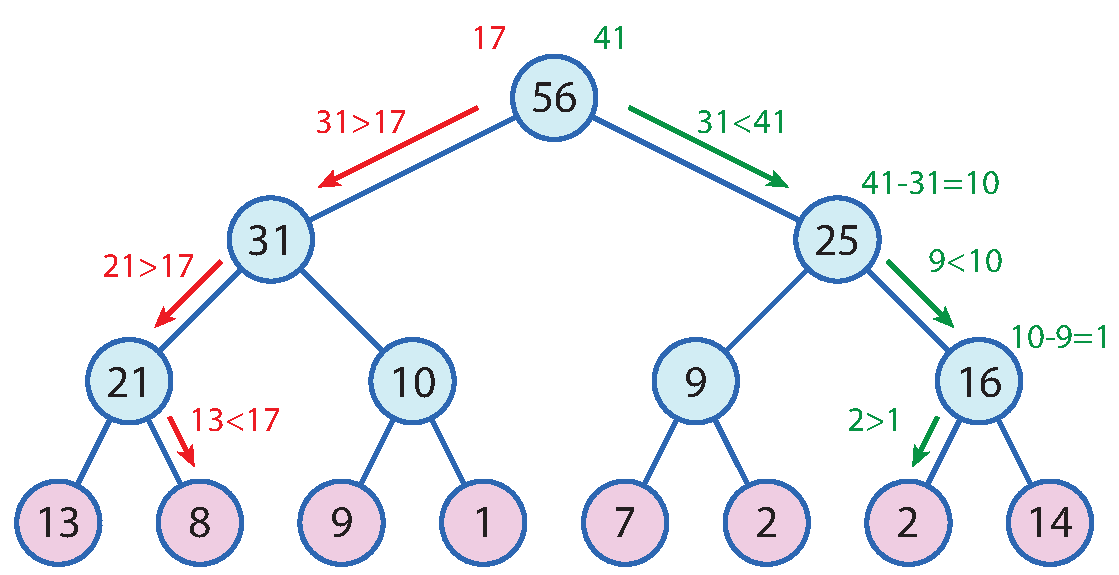
\includegraphics[width=\textwidth]{images/ddpg/sumtree.pdf}
\caption{The sumtree structure used in prioritization. Example traces are shown in red and green.}
\label{fig:sumtree}
\end{figure}

Implementation was done in a heap-like array, where index $i$ is parent to nodes $2i+1, 2i+2$. The complexity of adding, replacing and updating a node is $O(\log_2N)$.

For comparison between uniform and proportional distributions, see \ref{plot:prior}. The proportional version is able to find better solutions faster.
\begin{figure}[htbp]
%% Creator: Matplotlib, PGF backend
%%
%% To include the figure in your LaTeX document, write
%%   \input{<filename>.pgf}
%%
%% Make sure the required packages are loaded in your preamble
%%   \usepackage{pgf}
%%
%% Figures using additional raster images can only be included by \input if
%% they are in the same directory as the main LaTeX file. For loading figures
%% from other directories you can use the `import` package
%%   \usepackage{import}
%% and then include the figures with
%%   \import{<path to file>}{<filename>.pgf}
%%
%% Matplotlib used the following preamble
%%   \usepackage[utf8x]{inputenc}
%%   \usepackage[T1]{fontenc}
%%
\begingroup%
\makeatletter%
\begin{pgfpicture}%
\pgfpathrectangle{\pgfpointorigin}{\pgfqpoint{5.022831in}{2.009132in}}%
\pgfusepath{use as bounding box, clip}%
\begin{pgfscope}%
\pgfsetbuttcap%
\pgfsetmiterjoin%
\definecolor{currentfill}{rgb}{1.000000,1.000000,1.000000}%
\pgfsetfillcolor{currentfill}%
\pgfsetlinewidth{0.000000pt}%
\definecolor{currentstroke}{rgb}{1.000000,1.000000,1.000000}%
\pgfsetstrokecolor{currentstroke}%
\pgfsetdash{}{0pt}%
\pgfpathmoveto{\pgfqpoint{0.000000in}{0.000000in}}%
\pgfpathlineto{\pgfqpoint{5.022831in}{0.000000in}}%
\pgfpathlineto{\pgfqpoint{5.022831in}{2.009132in}}%
\pgfpathlineto{\pgfqpoint{0.000000in}{2.009132in}}%
\pgfpathclose%
\pgfusepath{fill}%
\end{pgfscope}%
\begin{pgfscope}%
\pgfsetbuttcap%
\pgfsetmiterjoin%
\definecolor{currentfill}{rgb}{1.000000,1.000000,1.000000}%
\pgfsetfillcolor{currentfill}%
\pgfsetlinewidth{0.000000pt}%
\definecolor{currentstroke}{rgb}{0.000000,0.000000,0.000000}%
\pgfsetstrokecolor{currentstroke}%
\pgfsetstrokeopacity{0.000000}%
\pgfsetdash{}{0pt}%
\pgfpathmoveto{\pgfqpoint{0.607535in}{0.495779in}}%
\pgfpathlineto{\pgfqpoint{4.754774in}{0.495779in}}%
\pgfpathlineto{\pgfqpoint{4.754774in}{1.810070in}}%
\pgfpathlineto{\pgfqpoint{0.607535in}{1.810070in}}%
\pgfpathclose%
\pgfusepath{fill}%
\end{pgfscope}%
\begin{pgfscope}%
\pgfpathrectangle{\pgfqpoint{0.607535in}{0.495779in}}{\pgfqpoint{4.147239in}{1.314291in}} %
\pgfusepath{clip}%
\pgfsetrectcap%
\pgfsetroundjoin%
\pgfsetlinewidth{0.501875pt}%
\definecolor{currentstroke}{rgb}{0.000000,0.000000,1.000000}%
\pgfsetstrokecolor{currentstroke}%
\pgfsetdash{}{0pt}%
\pgfpathmoveto{\pgfqpoint{0.607336in}{0.672753in}}%
\pgfpathlineto{\pgfqpoint{0.616224in}{0.684585in}}%
\pgfpathlineto{\pgfqpoint{0.639581in}{0.684487in}}%
\pgfpathlineto{\pgfqpoint{0.643038in}{0.708881in}}%
\pgfpathlineto{\pgfqpoint{0.648342in}{0.805436in}}%
\pgfpathlineto{\pgfqpoint{0.655241in}{0.793123in}}%
\pgfpathlineto{\pgfqpoint{0.661830in}{0.797659in}}%
\pgfpathlineto{\pgfqpoint{0.668980in}{0.807133in}}%
\pgfpathlineto{\pgfqpoint{0.675111in}{0.810921in}}%
\pgfpathlineto{\pgfqpoint{0.695007in}{0.816315in}}%
\pgfpathlineto{\pgfqpoint{0.702614in}{0.812948in}}%
\pgfpathlineto{\pgfqpoint{0.710081in}{0.818478in}}%
\pgfpathlineto{\pgfqpoint{0.722835in}{0.824874in}}%
\pgfpathlineto{\pgfqpoint{0.729337in}{0.832737in}}%
\pgfpathlineto{\pgfqpoint{0.736199in}{0.819710in}}%
\pgfpathlineto{\pgfqpoint{0.742998in}{0.820271in}}%
\pgfpathlineto{\pgfqpoint{0.749709in}{0.798709in}}%
\pgfpathlineto{\pgfqpoint{0.757006in}{0.794201in}}%
\pgfpathlineto{\pgfqpoint{0.763398in}{0.797754in}}%
\pgfpathlineto{\pgfqpoint{0.770571in}{0.804652in}}%
\pgfpathlineto{\pgfqpoint{0.777893in}{0.799149in}}%
\pgfpathlineto{\pgfqpoint{0.785529in}{0.801118in}}%
\pgfpathlineto{\pgfqpoint{0.792926in}{0.798938in}}%
\pgfpathlineto{\pgfqpoint{0.801015in}{0.812080in}}%
\pgfpathlineto{\pgfqpoint{0.810033in}{0.807969in}}%
\pgfpathlineto{\pgfqpoint{0.833287in}{1.016893in}}%
\pgfpathlineto{\pgfqpoint{0.862081in}{1.229399in}}%
\pgfpathlineto{\pgfqpoint{0.891926in}{1.196091in}}%
\pgfpathlineto{\pgfqpoint{0.921771in}{1.249411in}}%
\pgfpathlineto{\pgfqpoint{0.951616in}{1.219034in}}%
\pgfpathlineto{\pgfqpoint{0.979370in}{1.234135in}}%
\pgfpathlineto{\pgfqpoint{1.009215in}{1.301430in}}%
\pgfpathlineto{\pgfqpoint{1.039060in}{1.196829in}}%
\pgfpathlineto{\pgfqpoint{1.068905in}{1.282097in}}%
\pgfpathlineto{\pgfqpoint{1.098750in}{1.253794in}}%
\pgfpathlineto{\pgfqpoint{1.158441in}{1.306844in}}%
\pgfpathlineto{\pgfqpoint{1.181249in}{0.837763in}}%
\pgfpathlineto{\pgfqpoint{1.204594in}{1.050988in}}%
\pgfpathlineto{\pgfqpoint{1.234440in}{1.242898in}}%
\pgfpathlineto{\pgfqpoint{1.264285in}{1.313985in}}%
\pgfpathlineto{\pgfqpoint{1.293171in}{1.215005in}}%
\pgfpathlineto{\pgfqpoint{1.323016in}{1.237807in}}%
\pgfpathlineto{\pgfqpoint{1.352862in}{1.273928in}}%
\pgfpathlineto{\pgfqpoint{1.382707in}{1.276666in}}%
\pgfpathlineto{\pgfqpoint{1.412552in}{1.242019in}}%
\pgfpathlineto{\pgfqpoint{1.442397in}{1.294739in}}%
\pgfpathlineto{\pgfqpoint{1.472242in}{1.301492in}}%
\pgfpathlineto{\pgfqpoint{1.502088in}{1.296005in}}%
\pgfpathlineto{\pgfqpoint{1.531933in}{1.318168in}}%
\pgfpathlineto{\pgfqpoint{1.561778in}{1.306137in}}%
\pgfpathlineto{\pgfqpoint{1.589543in}{1.309075in}}%
\pgfpathlineto{\pgfqpoint{1.617628in}{1.315046in}}%
\pgfpathlineto{\pgfqpoint{1.647473in}{1.374169in}}%
\pgfpathlineto{\pgfqpoint{1.677318in}{1.347861in}}%
\pgfpathlineto{\pgfqpoint{1.707164in}{1.367593in}}%
\pgfpathlineto{\pgfqpoint{1.737009in}{1.362871in}}%
\pgfpathlineto{\pgfqpoint{1.766854in}{1.319794in}}%
\pgfpathlineto{\pgfqpoint{1.796699in}{1.389866in}}%
\pgfpathlineto{\pgfqpoint{1.826544in}{1.367503in}}%
\pgfpathlineto{\pgfqpoint{1.856390in}{1.313922in}}%
\pgfpathlineto{\pgfqpoint{1.886235in}{1.380005in}}%
\pgfpathlineto{\pgfqpoint{1.916080in}{1.367817in}}%
\pgfpathlineto{\pgfqpoint{1.945925in}{1.369450in}}%
\pgfpathlineto{\pgfqpoint{2.005615in}{1.195972in}}%
\pgfpathlineto{\pgfqpoint{2.035461in}{1.345672in}}%
\pgfpathlineto{\pgfqpoint{2.065306in}{1.374997in}}%
\pgfpathlineto{\pgfqpoint{2.095151in}{1.402016in}}%
\pgfpathlineto{\pgfqpoint{2.124996in}{1.302666in}}%
\pgfpathlineto{\pgfqpoint{2.152013in}{1.364753in}}%
\pgfpathlineto{\pgfqpoint{2.181858in}{1.368924in}}%
\pgfpathlineto{\pgfqpoint{2.211703in}{1.307328in}}%
\pgfpathlineto{\pgfqpoint{2.241549in}{1.295787in}}%
\pgfpathlineto{\pgfqpoint{2.271394in}{1.355342in}}%
\pgfpathlineto{\pgfqpoint{2.301239in}{1.341418in}}%
\pgfpathlineto{\pgfqpoint{2.331084in}{1.366378in}}%
\pgfpathlineto{\pgfqpoint{2.360929in}{1.355522in}}%
\pgfpathlineto{\pgfqpoint{2.390775in}{1.371257in}}%
\pgfpathlineto{\pgfqpoint{2.420620in}{1.344009in}}%
\pgfpathlineto{\pgfqpoint{2.447529in}{1.359116in}}%
\pgfpathlineto{\pgfqpoint{2.477374in}{1.327255in}}%
\pgfpathlineto{\pgfqpoint{2.507219in}{1.392652in}}%
\pgfpathlineto{\pgfqpoint{2.537064in}{1.391615in}}%
\pgfpathlineto{\pgfqpoint{2.566909in}{1.383240in}}%
\pgfpathlineto{\pgfqpoint{2.596755in}{1.381980in}}%
\pgfpathlineto{\pgfqpoint{2.626600in}{1.388378in}}%
\pgfpathlineto{\pgfqpoint{2.656445in}{1.380672in}}%
\pgfpathlineto{\pgfqpoint{2.686290in}{1.345967in}}%
\pgfpathlineto{\pgfqpoint{2.716135in}{1.327700in}}%
\pgfpathlineto{\pgfqpoint{2.745981in}{1.264167in}}%
\pgfpathlineto{\pgfqpoint{2.773706in}{1.261508in}}%
\pgfpathlineto{\pgfqpoint{2.803551in}{1.302355in}}%
\pgfpathlineto{\pgfqpoint{2.833396in}{1.333815in}}%
\pgfpathlineto{\pgfqpoint{2.863241in}{1.313048in}}%
\pgfpathlineto{\pgfqpoint{2.891436in}{1.335240in}}%
\pgfpathlineto{\pgfqpoint{2.921281in}{1.406507in}}%
\pgfpathlineto{\pgfqpoint{2.951126in}{1.385625in}}%
\pgfpathlineto{\pgfqpoint{2.980971in}{1.396569in}}%
\pgfpathlineto{\pgfqpoint{3.010817in}{1.361141in}}%
\pgfpathlineto{\pgfqpoint{3.040662in}{1.320708in}}%
\pgfpathlineto{\pgfqpoint{3.100352in}{1.344797in}}%
\pgfpathlineto{\pgfqpoint{3.129431in}{1.419712in}}%
\pgfpathlineto{\pgfqpoint{3.156994in}{1.310338in}}%
\pgfpathlineto{\pgfqpoint{3.180800in}{1.618296in}}%
\pgfpathlineto{\pgfqpoint{3.207799in}{1.570825in}}%
\pgfpathlineto{\pgfqpoint{3.233756in}{1.365033in}}%
\pgfpathlineto{\pgfqpoint{3.257045in}{1.435381in}}%
\pgfpathlineto{\pgfqpoint{3.285334in}{1.608371in}}%
\pgfpathlineto{\pgfqpoint{3.302255in}{0.748234in}}%
\pgfpathlineto{\pgfqpoint{3.320841in}{1.398714in}}%
\pgfpathlineto{\pgfqpoint{3.344233in}{1.590113in}}%
\pgfpathlineto{\pgfqpoint{3.374078in}{1.351973in}}%
\pgfpathlineto{\pgfqpoint{3.403923in}{1.508154in}}%
\pgfpathlineto{\pgfqpoint{3.433769in}{1.259214in}}%
\pgfpathlineto{\pgfqpoint{3.463614in}{1.470809in}}%
\pgfpathlineto{\pgfqpoint{3.481875in}{1.417973in}}%
\pgfpathlineto{\pgfqpoint{3.508489in}{1.576342in}}%
\pgfpathlineto{\pgfqpoint{3.536806in}{1.541778in}}%
\pgfpathlineto{\pgfqpoint{3.565166in}{1.636766in}}%
\pgfpathlineto{\pgfqpoint{3.593937in}{1.543339in}}%
\pgfpathlineto{\pgfqpoint{3.621906in}{1.490153in}}%
\pgfpathlineto{\pgfqpoint{3.648057in}{1.527186in}}%
\pgfpathlineto{\pgfqpoint{3.669582in}{0.972422in}}%
\pgfpathlineto{\pgfqpoint{3.696858in}{0.950739in}}%
\pgfpathlineto{\pgfqpoint{3.715418in}{1.011971in}}%
\pgfpathlineto{\pgfqpoint{3.740477in}{1.380477in}}%
\pgfpathlineto{\pgfqpoint{3.763429in}{1.051228in}}%
\pgfpathlineto{\pgfqpoint{3.789559in}{1.646635in}}%
\pgfpathlineto{\pgfqpoint{3.813488in}{1.251788in}}%
\pgfpathlineto{\pgfqpoint{3.837889in}{1.508772in}}%
\pgfpathlineto{\pgfqpoint{3.863743in}{1.393221in}}%
\pgfpathlineto{\pgfqpoint{3.885116in}{1.366174in}}%
\pgfpathlineto{\pgfqpoint{3.908788in}{1.399881in}}%
\pgfpathlineto{\pgfqpoint{3.924855in}{1.072225in}}%
\pgfpathlineto{\pgfqpoint{3.947107in}{1.379485in}}%
\pgfpathlineto{\pgfqpoint{3.959967in}{1.231613in}}%
\pgfpathlineto{\pgfqpoint{3.985561in}{1.275629in}}%
\pgfpathlineto{\pgfqpoint{4.010797in}{1.610653in}}%
\pgfpathlineto{\pgfqpoint{4.028144in}{1.312825in}}%
\pgfpathlineto{\pgfqpoint{4.053187in}{1.259836in}}%
\pgfpathlineto{\pgfqpoint{4.076262in}{1.427863in}}%
\pgfpathlineto{\pgfqpoint{4.096040in}{1.162883in}}%
\pgfpathlineto{\pgfqpoint{4.118254in}{1.015936in}}%
\pgfpathlineto{\pgfqpoint{4.143117in}{1.582779in}}%
\pgfpathlineto{\pgfqpoint{4.166611in}{1.691435in}}%
\pgfpathlineto{\pgfqpoint{4.190968in}{1.698754in}}%
\pgfpathlineto{\pgfqpoint{4.199691in}{1.304634in}}%
\pgfpathlineto{\pgfqpoint{4.222592in}{1.419293in}}%
\pgfpathlineto{\pgfqpoint{4.247562in}{1.022371in}}%
\pgfpathlineto{\pgfqpoint{4.267503in}{1.572851in}}%
\pgfpathlineto{\pgfqpoint{4.290967in}{1.417399in}}%
\pgfpathlineto{\pgfqpoint{4.309820in}{1.618240in}}%
\pgfpathlineto{\pgfqpoint{4.324899in}{0.900005in}}%
\pgfpathlineto{\pgfqpoint{4.338776in}{0.978315in}}%
\pgfpathlineto{\pgfqpoint{4.354104in}{0.952704in}}%
\pgfpathlineto{\pgfqpoint{4.375073in}{1.230233in}}%
\pgfpathlineto{\pgfqpoint{4.392083in}{1.425578in}}%
\pgfpathlineto{\pgfqpoint{4.409851in}{1.283658in}}%
\pgfpathlineto{\pgfqpoint{4.431176in}{1.532722in}}%
\pgfpathlineto{\pgfqpoint{4.449965in}{1.529422in}}%
\pgfpathlineto{\pgfqpoint{4.467632in}{1.704976in}}%
\pgfpathlineto{\pgfqpoint{4.489435in}{1.657358in}}%
\pgfpathlineto{\pgfqpoint{4.503949in}{0.963086in}}%
\pgfpathlineto{\pgfqpoint{4.519615in}{1.710468in}}%
\pgfpathlineto{\pgfqpoint{4.534949in}{1.130224in}}%
\pgfpathlineto{\pgfqpoint{4.547097in}{1.513946in}}%
\pgfpathlineto{\pgfqpoint{4.563734in}{0.931024in}}%
\pgfpathlineto{\pgfqpoint{4.576001in}{0.952992in}}%
\pgfpathlineto{\pgfqpoint{4.596502in}{0.931121in}}%
\pgfpathlineto{\pgfqpoint{4.610022in}{1.098969in}}%
\pgfpathlineto{\pgfqpoint{4.626024in}{1.008317in}}%
\pgfpathlineto{\pgfqpoint{4.641234in}{1.049767in}}%
\pgfpathlineto{\pgfqpoint{4.654238in}{1.642921in}}%
\pgfpathlineto{\pgfqpoint{4.669747in}{1.056400in}}%
\pgfpathlineto{\pgfqpoint{4.683176in}{1.171459in}}%
\pgfpathlineto{\pgfqpoint{4.697379in}{1.148176in}}%
\pgfpathlineto{\pgfqpoint{4.715504in}{1.620270in}}%
\pgfpathlineto{\pgfqpoint{4.733847in}{1.187625in}}%
\pgfpathlineto{\pgfqpoint{4.748941in}{0.953802in}}%
\pgfpathlineto{\pgfqpoint{4.764498in}{1.060755in}}%
\pgfpathlineto{\pgfqpoint{4.764498in}{1.060755in}}%
\pgfusepath{stroke}%
\end{pgfscope}%
\begin{pgfscope}%
\pgfpathrectangle{\pgfqpoint{0.607535in}{0.495779in}}{\pgfqpoint{4.147239in}{1.314291in}} %
\pgfusepath{clip}%
\pgfsetrectcap%
\pgfsetroundjoin%
\pgfsetlinewidth{0.501875pt}%
\definecolor{currentstroke}{rgb}{0.000000,0.500000,0.000000}%
\pgfsetstrokecolor{currentstroke}%
\pgfsetdash{}{0pt}%
\pgfpathmoveto{\pgfqpoint{0.603606in}{0.673292in}}%
\pgfpathlineto{\pgfqpoint{0.610352in}{0.684637in}}%
\pgfpathlineto{\pgfqpoint{0.616324in}{0.684572in}}%
\pgfpathlineto{\pgfqpoint{0.621746in}{0.704614in}}%
\pgfpathlineto{\pgfqpoint{0.625809in}{0.684572in}}%
\pgfpathlineto{\pgfqpoint{0.628744in}{0.684568in}}%
\pgfpathlineto{\pgfqpoint{0.633563in}{0.708784in}}%
\pgfpathlineto{\pgfqpoint{0.639133in}{0.709521in}}%
\pgfpathlineto{\pgfqpoint{0.643916in}{0.723737in}}%
\pgfpathlineto{\pgfqpoint{0.647629in}{0.703903in}}%
\pgfpathlineto{\pgfqpoint{0.654191in}{0.714765in}}%
\pgfpathlineto{\pgfqpoint{0.661140in}{0.723282in}}%
\pgfpathlineto{\pgfqpoint{0.668461in}{0.715184in}}%
\pgfpathlineto{\pgfqpoint{0.689103in}{0.736872in}}%
\pgfpathlineto{\pgfqpoint{0.696516in}{0.750170in}}%
\pgfpathlineto{\pgfqpoint{0.706647in}{0.830973in}}%
\pgfpathlineto{\pgfqpoint{0.725910in}{0.831897in}}%
\pgfpathlineto{\pgfqpoint{0.734454in}{0.826332in}}%
\pgfpathlineto{\pgfqpoint{0.743236in}{0.824615in}}%
\pgfpathlineto{\pgfqpoint{0.753549in}{0.842367in}}%
\pgfpathlineto{\pgfqpoint{0.766397in}{0.859169in}}%
\pgfpathlineto{\pgfqpoint{0.777135in}{0.823290in}}%
\pgfpathlineto{\pgfqpoint{0.785720in}{0.813128in}}%
\pgfpathlineto{\pgfqpoint{0.811962in}{0.802852in}}%
\pgfpathlineto{\pgfqpoint{0.832436in}{1.194063in}}%
\pgfpathlineto{\pgfqpoint{0.858632in}{0.930054in}}%
\pgfpathlineto{\pgfqpoint{0.887553in}{1.143898in}}%
\pgfpathlineto{\pgfqpoint{0.917398in}{1.225787in}}%
\pgfpathlineto{\pgfqpoint{0.947243in}{1.054954in}}%
\pgfpathlineto{\pgfqpoint{0.977089in}{1.122406in}}%
\pgfpathlineto{\pgfqpoint{1.006934in}{1.253778in}}%
\pgfpathlineto{\pgfqpoint{1.034841in}{1.231884in}}%
\pgfpathlineto{\pgfqpoint{1.064687in}{1.246404in}}%
\pgfpathlineto{\pgfqpoint{1.094532in}{1.227869in}}%
\pgfpathlineto{\pgfqpoint{1.124377in}{1.272554in}}%
\pgfpathlineto{\pgfqpoint{1.154222in}{1.217418in}}%
\pgfpathlineto{\pgfqpoint{1.184067in}{1.240363in}}%
\pgfpathlineto{\pgfqpoint{1.213405in}{1.220426in}}%
\pgfpathlineto{\pgfqpoint{1.243250in}{1.254832in}}%
\pgfpathlineto{\pgfqpoint{1.273095in}{1.218921in}}%
\pgfpathlineto{\pgfqpoint{1.302940in}{1.196759in}}%
\pgfpathlineto{\pgfqpoint{1.332786in}{1.198231in}}%
\pgfpathlineto{\pgfqpoint{1.360058in}{1.184192in}}%
\pgfpathlineto{\pgfqpoint{1.388025in}{1.267398in}}%
\pgfpathlineto{\pgfqpoint{1.415918in}{1.296487in}}%
\pgfpathlineto{\pgfqpoint{1.445763in}{1.228429in}}%
\pgfpathlineto{\pgfqpoint{1.475608in}{1.237591in}}%
\pgfpathlineto{\pgfqpoint{1.503219in}{1.325834in}}%
\pgfpathlineto{\pgfqpoint{1.533064in}{1.281526in}}%
\pgfpathlineto{\pgfqpoint{1.590075in}{1.351169in}}%
\pgfpathlineto{\pgfqpoint{1.619921in}{1.258282in}}%
\pgfpathlineto{\pgfqpoint{1.649766in}{1.237583in}}%
\pgfpathlineto{\pgfqpoint{1.679611in}{1.190505in}}%
\pgfpathlineto{\pgfqpoint{1.709456in}{1.376479in}}%
\pgfpathlineto{\pgfqpoint{1.739301in}{1.363924in}}%
\pgfpathlineto{\pgfqpoint{1.769147in}{1.383309in}}%
\pgfpathlineto{\pgfqpoint{1.798992in}{1.390480in}}%
\pgfpathlineto{\pgfqpoint{1.828837in}{1.298547in}}%
\pgfpathlineto{\pgfqpoint{1.858682in}{1.377855in}}%
\pgfpathlineto{\pgfqpoint{1.888527in}{1.215911in}}%
\pgfpathlineto{\pgfqpoint{1.918372in}{1.222565in}}%
\pgfpathlineto{\pgfqpoint{1.947403in}{1.441324in}}%
\pgfpathlineto{\pgfqpoint{1.973284in}{1.268029in}}%
\pgfpathlineto{\pgfqpoint{1.994856in}{1.289191in}}%
\pgfpathlineto{\pgfqpoint{2.020255in}{1.174773in}}%
\pgfpathlineto{\pgfqpoint{2.047702in}{1.294647in}}%
\pgfpathlineto{\pgfqpoint{2.076004in}{1.197618in}}%
\pgfpathlineto{\pgfqpoint{2.105849in}{1.221091in}}%
\pgfpathlineto{\pgfqpoint{2.135694in}{0.891710in}}%
\pgfpathlineto{\pgfqpoint{2.163308in}{1.025329in}}%
\pgfpathlineto{\pgfqpoint{2.178448in}{0.872796in}}%
\pgfpathlineto{\pgfqpoint{2.196647in}{0.784626in}}%
\pgfpathlineto{\pgfqpoint{2.217969in}{1.433399in}}%
\pgfpathlineto{\pgfqpoint{2.236746in}{1.088869in}}%
\pgfpathlineto{\pgfqpoint{2.257914in}{1.253452in}}%
\pgfpathlineto{\pgfqpoint{2.279439in}{1.451880in}}%
\pgfpathlineto{\pgfqpoint{2.300756in}{1.342802in}}%
\pgfpathlineto{\pgfqpoint{2.316053in}{0.825935in}}%
\pgfpathlineto{\pgfqpoint{2.328251in}{1.354687in}}%
\pgfpathlineto{\pgfqpoint{2.337025in}{1.098351in}}%
\pgfpathlineto{\pgfqpoint{2.350891in}{0.772988in}}%
\pgfpathlineto{\pgfqpoint{2.355913in}{0.776153in}}%
\pgfpathlineto{\pgfqpoint{2.364478in}{0.776591in}}%
\pgfpathlineto{\pgfqpoint{2.375050in}{0.791751in}}%
\pgfpathlineto{\pgfqpoint{2.385385in}{0.814853in}}%
\pgfpathlineto{\pgfqpoint{2.393334in}{0.794719in}}%
\pgfpathlineto{\pgfqpoint{2.405265in}{0.843363in}}%
\pgfpathlineto{\pgfqpoint{2.418314in}{0.904615in}}%
\pgfpathlineto{\pgfqpoint{2.435956in}{0.784595in}}%
\pgfpathlineto{\pgfqpoint{2.446673in}{0.843591in}}%
\pgfpathlineto{\pgfqpoint{2.451231in}{0.737226in}}%
\pgfpathlineto{\pgfqpoint{2.461976in}{0.778913in}}%
\pgfpathlineto{\pgfqpoint{2.485265in}{1.579339in}}%
\pgfpathlineto{\pgfqpoint{2.505031in}{1.672797in}}%
\pgfpathlineto{\pgfqpoint{2.529261in}{1.657450in}}%
\pgfpathlineto{\pgfqpoint{2.555025in}{1.653424in}}%
\pgfpathlineto{\pgfqpoint{2.572545in}{0.870821in}}%
\pgfpathlineto{\pgfqpoint{2.599857in}{1.634004in}}%
\pgfpathlineto{\pgfqpoint{2.629702in}{1.646041in}}%
\pgfpathlineto{\pgfqpoint{2.659547in}{1.716477in}}%
\pgfpathlineto{\pgfqpoint{2.689170in}{1.411066in}}%
\pgfpathlineto{\pgfqpoint{2.706409in}{0.932987in}}%
\pgfpathlineto{\pgfqpoint{2.718478in}{0.926478in}}%
\pgfpathlineto{\pgfqpoint{2.726421in}{0.919462in}}%
\pgfpathlineto{\pgfqpoint{2.734838in}{0.910356in}}%
\pgfpathlineto{\pgfqpoint{2.744177in}{0.912357in}}%
\pgfpathlineto{\pgfqpoint{2.755421in}{0.983316in}}%
\pgfpathlineto{\pgfqpoint{2.767850in}{0.959215in}}%
\pgfpathlineto{\pgfqpoint{2.789649in}{1.597417in}}%
\pgfpathlineto{\pgfqpoint{2.804725in}{1.583135in}}%
\pgfpathlineto{\pgfqpoint{2.824320in}{0.853895in}}%
\pgfpathlineto{\pgfqpoint{2.840702in}{0.804190in}}%
\pgfpathlineto{\pgfqpoint{2.850703in}{0.807197in}}%
\pgfpathlineto{\pgfqpoint{2.867483in}{0.808913in}}%
\pgfpathlineto{\pgfqpoint{2.885689in}{0.940996in}}%
\pgfpathlineto{\pgfqpoint{2.894337in}{0.920937in}}%
\pgfpathlineto{\pgfqpoint{2.903129in}{0.891877in}}%
\pgfpathlineto{\pgfqpoint{2.911300in}{0.811600in}}%
\pgfpathlineto{\pgfqpoint{2.919151in}{0.805382in}}%
\pgfpathlineto{\pgfqpoint{2.925986in}{0.785935in}}%
\pgfpathlineto{\pgfqpoint{2.933321in}{0.800539in}}%
\pgfpathlineto{\pgfqpoint{2.941787in}{0.831525in}}%
\pgfpathlineto{\pgfqpoint{2.949091in}{0.833447in}}%
\pgfpathlineto{\pgfqpoint{2.966755in}{0.949688in}}%
\pgfpathlineto{\pgfqpoint{2.979279in}{0.813030in}}%
\pgfpathlineto{\pgfqpoint{2.995701in}{0.921955in}}%
\pgfpathlineto{\pgfqpoint{3.014207in}{1.108090in}}%
\pgfpathlineto{\pgfqpoint{3.022830in}{0.855174in}}%
\pgfpathlineto{\pgfqpoint{3.033371in}{0.886358in}}%
\pgfpathlineto{\pgfqpoint{3.043729in}{0.978345in}}%
\pgfpathlineto{\pgfqpoint{3.053958in}{0.871119in}}%
\pgfpathlineto{\pgfqpoint{3.067448in}{1.510730in}}%
\pgfpathlineto{\pgfqpoint{3.085006in}{0.953814in}}%
\pgfpathlineto{\pgfqpoint{3.099770in}{0.943093in}}%
\pgfpathlineto{\pgfqpoint{3.111551in}{0.920050in}}%
\pgfpathlineto{\pgfqpoint{3.121818in}{0.993124in}}%
\pgfpathlineto{\pgfqpoint{3.135352in}{0.946425in}}%
\pgfpathlineto{\pgfqpoint{3.148039in}{0.961591in}}%
\pgfpathlineto{\pgfqpoint{3.166122in}{0.867432in}}%
\pgfpathlineto{\pgfqpoint{3.178937in}{0.891107in}}%
\pgfpathlineto{\pgfqpoint{3.191338in}{1.382972in}}%
\pgfpathlineto{\pgfqpoint{3.211057in}{1.296871in}}%
\pgfpathlineto{\pgfqpoint{3.231227in}{0.989886in}}%
\pgfpathlineto{\pgfqpoint{3.245998in}{0.902045in}}%
\pgfpathlineto{\pgfqpoint{3.259029in}{1.167919in}}%
\pgfpathlineto{\pgfqpoint{3.276786in}{0.824603in}}%
\pgfpathlineto{\pgfqpoint{3.291689in}{0.927971in}}%
\pgfpathlineto{\pgfqpoint{3.305805in}{1.596143in}}%
\pgfpathlineto{\pgfqpoint{3.325352in}{1.495164in}}%
\pgfpathlineto{\pgfqpoint{3.339241in}{0.814171in}}%
\pgfpathlineto{\pgfqpoint{3.355724in}{0.962969in}}%
\pgfpathlineto{\pgfqpoint{3.375512in}{0.870799in}}%
\pgfpathlineto{\pgfqpoint{3.398525in}{1.562738in}}%
\pgfpathlineto{\pgfqpoint{3.414663in}{1.555893in}}%
\pgfpathlineto{\pgfqpoint{3.430554in}{0.821111in}}%
\pgfpathlineto{\pgfqpoint{3.441264in}{1.538941in}}%
\pgfpathlineto{\pgfqpoint{3.463448in}{1.580458in}}%
\pgfpathlineto{\pgfqpoint{3.475409in}{1.098631in}}%
\pgfpathlineto{\pgfqpoint{3.492638in}{1.093231in}}%
\pgfpathlineto{\pgfqpoint{3.510171in}{1.612182in}}%
\pgfpathlineto{\pgfqpoint{3.527967in}{1.578705in}}%
\pgfpathlineto{\pgfqpoint{3.545681in}{1.392666in}}%
\pgfpathlineto{\pgfqpoint{3.566094in}{1.400326in}}%
\pgfpathlineto{\pgfqpoint{3.592548in}{1.658696in}}%
\pgfpathlineto{\pgfqpoint{3.607852in}{1.651908in}}%
\pgfpathlineto{\pgfqpoint{3.627315in}{0.964531in}}%
\pgfpathlineto{\pgfqpoint{3.642577in}{1.697221in}}%
\pgfpathlineto{\pgfqpoint{3.656394in}{1.313376in}}%
\pgfpathlineto{\pgfqpoint{3.671170in}{0.998246in}}%
\pgfpathlineto{\pgfqpoint{3.685028in}{1.531828in}}%
\pgfpathlineto{\pgfqpoint{3.710031in}{1.600193in}}%
\pgfpathlineto{\pgfqpoint{3.727058in}{1.505788in}}%
\pgfpathlineto{\pgfqpoint{3.752519in}{1.600739in}}%
\pgfpathlineto{\pgfqpoint{3.778615in}{1.651478in}}%
\pgfpathlineto{\pgfqpoint{3.797321in}{1.134308in}}%
\pgfpathlineto{\pgfqpoint{3.824263in}{1.616968in}}%
\pgfpathlineto{\pgfqpoint{3.844959in}{1.110195in}}%
\pgfpathlineto{\pgfqpoint{3.858947in}{1.153040in}}%
\pgfpathlineto{\pgfqpoint{3.874708in}{1.078652in}}%
\pgfpathlineto{\pgfqpoint{3.898709in}{1.638527in}}%
\pgfpathlineto{\pgfqpoint{3.919405in}{1.641720in}}%
\pgfpathlineto{\pgfqpoint{3.938133in}{1.647141in}}%
\pgfpathlineto{\pgfqpoint{3.954546in}{1.158751in}}%
\pgfpathlineto{\pgfqpoint{3.970406in}{0.847063in}}%
\pgfpathlineto{\pgfqpoint{3.984774in}{1.029235in}}%
\pgfpathlineto{\pgfqpoint{3.999683in}{0.821519in}}%
\pgfpathlineto{\pgfqpoint{4.014578in}{0.819901in}}%
\pgfpathlineto{\pgfqpoint{4.031213in}{0.772797in}}%
\pgfpathlineto{\pgfqpoint{4.048862in}{1.597266in}}%
\pgfpathlineto{\pgfqpoint{4.070008in}{1.333547in}}%
\pgfpathlineto{\pgfqpoint{4.082193in}{1.324276in}}%
\pgfpathlineto{\pgfqpoint{4.091755in}{1.102936in}}%
\pgfpathlineto{\pgfqpoint{4.106998in}{0.779322in}}%
\pgfpathlineto{\pgfqpoint{4.128214in}{1.612956in}}%
\pgfpathlineto{\pgfqpoint{4.144506in}{0.937633in}}%
\pgfpathlineto{\pgfqpoint{4.157279in}{0.809021in}}%
\pgfpathlineto{\pgfqpoint{4.169452in}{0.838206in}}%
\pgfpathlineto{\pgfqpoint{4.181425in}{0.777430in}}%
\pgfpathlineto{\pgfqpoint{4.188180in}{0.788179in}}%
\pgfpathlineto{\pgfqpoint{4.199153in}{0.835403in}}%
\pgfpathlineto{\pgfqpoint{4.212016in}{1.475821in}}%
\pgfpathlineto{\pgfqpoint{4.228856in}{1.614506in}}%
\pgfpathlineto{\pgfqpoint{4.241274in}{0.899153in}}%
\pgfpathlineto{\pgfqpoint{4.254205in}{0.926585in}}%
\pgfpathlineto{\pgfqpoint{4.271813in}{1.103262in}}%
\pgfpathlineto{\pgfqpoint{4.290064in}{1.718952in}}%
\pgfpathlineto{\pgfqpoint{4.314533in}{1.717211in}}%
\pgfpathlineto{\pgfqpoint{4.335223in}{1.474668in}}%
\pgfpathlineto{\pgfqpoint{4.349990in}{1.159136in}}%
\pgfpathlineto{\pgfqpoint{4.349990in}{1.159136in}}%
\pgfusepath{stroke}%
\end{pgfscope}%
\begin{pgfscope}%
\pgfsetrectcap%
\pgfsetmiterjoin%
\pgfsetlinewidth{1.003750pt}%
\definecolor{currentstroke}{rgb}{0.000000,0.000000,0.000000}%
\pgfsetstrokecolor{currentstroke}%
\pgfsetdash{}{0pt}%
\pgfpathmoveto{\pgfqpoint{0.607535in}{1.810070in}}%
\pgfpathlineto{\pgfqpoint{4.754774in}{1.810070in}}%
\pgfusepath{stroke}%
\end{pgfscope}%
\begin{pgfscope}%
\pgfsetrectcap%
\pgfsetmiterjoin%
\pgfsetlinewidth{1.003750pt}%
\definecolor{currentstroke}{rgb}{0.000000,0.000000,0.000000}%
\pgfsetstrokecolor{currentstroke}%
\pgfsetdash{}{0pt}%
\pgfpathmoveto{\pgfqpoint{4.754774in}{0.495779in}}%
\pgfpathlineto{\pgfqpoint{4.754774in}{1.810070in}}%
\pgfusepath{stroke}%
\end{pgfscope}%
\begin{pgfscope}%
\pgfsetrectcap%
\pgfsetmiterjoin%
\pgfsetlinewidth{1.003750pt}%
\definecolor{currentstroke}{rgb}{0.000000,0.000000,0.000000}%
\pgfsetstrokecolor{currentstroke}%
\pgfsetdash{}{0pt}%
\pgfpathmoveto{\pgfqpoint{0.607535in}{0.495779in}}%
\pgfpathlineto{\pgfqpoint{4.754774in}{0.495779in}}%
\pgfusepath{stroke}%
\end{pgfscope}%
\begin{pgfscope}%
\pgfsetrectcap%
\pgfsetmiterjoin%
\pgfsetlinewidth{1.003750pt}%
\definecolor{currentstroke}{rgb}{0.000000,0.000000,0.000000}%
\pgfsetstrokecolor{currentstroke}%
\pgfsetdash{}{0pt}%
\pgfpathmoveto{\pgfqpoint{0.607535in}{0.495779in}}%
\pgfpathlineto{\pgfqpoint{0.607535in}{1.810070in}}%
\pgfusepath{stroke}%
\end{pgfscope}%
\begin{pgfscope}%
\pgfpathrectangle{\pgfqpoint{0.607535in}{0.495779in}}{\pgfqpoint{4.147239in}{1.314291in}} %
\pgfusepath{clip}%
\pgfsetbuttcap%
\pgfsetroundjoin%
\pgfsetlinewidth{0.501875pt}%
\definecolor{currentstroke}{rgb}{0.000000,0.000000,0.000000}%
\pgfsetstrokecolor{currentstroke}%
\pgfsetdash{{1.000000pt}{3.000000pt}}{0.000000pt}%
\pgfpathmoveto{\pgfqpoint{0.607535in}{0.495779in}}%
\pgfpathlineto{\pgfqpoint{0.607535in}{1.810070in}}%
\pgfusepath{stroke}%
\end{pgfscope}%
\begin{pgfscope}%
\pgfsetbuttcap%
\pgfsetroundjoin%
\definecolor{currentfill}{rgb}{0.000000,0.000000,0.000000}%
\pgfsetfillcolor{currentfill}%
\pgfsetlinewidth{0.501875pt}%
\definecolor{currentstroke}{rgb}{0.000000,0.000000,0.000000}%
\pgfsetstrokecolor{currentstroke}%
\pgfsetdash{}{0pt}%
\pgfsys@defobject{currentmarker}{\pgfqpoint{0.000000in}{0.000000in}}{\pgfqpoint{0.000000in}{0.055556in}}{%
\pgfpathmoveto{\pgfqpoint{0.000000in}{0.000000in}}%
\pgfpathlineto{\pgfqpoint{0.000000in}{0.055556in}}%
\pgfusepath{stroke,fill}%
}%
\begin{pgfscope}%
\pgfsys@transformshift{0.607535in}{0.495779in}%
\pgfsys@useobject{currentmarker}{}%
\end{pgfscope}%
\end{pgfscope}%
\begin{pgfscope}%
\pgfsetbuttcap%
\pgfsetroundjoin%
\definecolor{currentfill}{rgb}{0.000000,0.000000,0.000000}%
\pgfsetfillcolor{currentfill}%
\pgfsetlinewidth{0.501875pt}%
\definecolor{currentstroke}{rgb}{0.000000,0.000000,0.000000}%
\pgfsetstrokecolor{currentstroke}%
\pgfsetdash{}{0pt}%
\pgfsys@defobject{currentmarker}{\pgfqpoint{0.000000in}{-0.055556in}}{\pgfqpoint{0.000000in}{0.000000in}}{%
\pgfpathmoveto{\pgfqpoint{0.000000in}{0.000000in}}%
\pgfpathlineto{\pgfqpoint{0.000000in}{-0.055556in}}%
\pgfusepath{stroke,fill}%
}%
\begin{pgfscope}%
\pgfsys@transformshift{0.607535in}{1.810070in}%
\pgfsys@useobject{currentmarker}{}%
\end{pgfscope}%
\end{pgfscope}%
\begin{pgfscope}%
\pgftext[x=0.607535in,y=0.440224in,,top]{\fontsize{8.000000}{9.600000}\selectfont \(\displaystyle 0\)}%
\end{pgfscope}%
\begin{pgfscope}%
\pgfpathrectangle{\pgfqpoint{0.607535in}{0.495779in}}{\pgfqpoint{4.147239in}{1.314291in}} %
\pgfusepath{clip}%
\pgfsetbuttcap%
\pgfsetroundjoin%
\pgfsetlinewidth{0.501875pt}%
\definecolor{currentstroke}{rgb}{0.000000,0.000000,0.000000}%
\pgfsetstrokecolor{currentstroke}%
\pgfsetdash{{1.000000pt}{3.000000pt}}{0.000000pt}%
\pgfpathmoveto{\pgfqpoint{1.436983in}{0.495779in}}%
\pgfpathlineto{\pgfqpoint{1.436983in}{1.810070in}}%
\pgfusepath{stroke}%
\end{pgfscope}%
\begin{pgfscope}%
\pgfsetbuttcap%
\pgfsetroundjoin%
\definecolor{currentfill}{rgb}{0.000000,0.000000,0.000000}%
\pgfsetfillcolor{currentfill}%
\pgfsetlinewidth{0.501875pt}%
\definecolor{currentstroke}{rgb}{0.000000,0.000000,0.000000}%
\pgfsetstrokecolor{currentstroke}%
\pgfsetdash{}{0pt}%
\pgfsys@defobject{currentmarker}{\pgfqpoint{0.000000in}{0.000000in}}{\pgfqpoint{0.000000in}{0.055556in}}{%
\pgfpathmoveto{\pgfqpoint{0.000000in}{0.000000in}}%
\pgfpathlineto{\pgfqpoint{0.000000in}{0.055556in}}%
\pgfusepath{stroke,fill}%
}%
\begin{pgfscope}%
\pgfsys@transformshift{1.436983in}{0.495779in}%
\pgfsys@useobject{currentmarker}{}%
\end{pgfscope}%
\end{pgfscope}%
\begin{pgfscope}%
\pgfsetbuttcap%
\pgfsetroundjoin%
\definecolor{currentfill}{rgb}{0.000000,0.000000,0.000000}%
\pgfsetfillcolor{currentfill}%
\pgfsetlinewidth{0.501875pt}%
\definecolor{currentstroke}{rgb}{0.000000,0.000000,0.000000}%
\pgfsetstrokecolor{currentstroke}%
\pgfsetdash{}{0pt}%
\pgfsys@defobject{currentmarker}{\pgfqpoint{0.000000in}{-0.055556in}}{\pgfqpoint{0.000000in}{0.000000in}}{%
\pgfpathmoveto{\pgfqpoint{0.000000in}{0.000000in}}%
\pgfpathlineto{\pgfqpoint{0.000000in}{-0.055556in}}%
\pgfusepath{stroke,fill}%
}%
\begin{pgfscope}%
\pgfsys@transformshift{1.436983in}{1.810070in}%
\pgfsys@useobject{currentmarker}{}%
\end{pgfscope}%
\end{pgfscope}%
\begin{pgfscope}%
\pgftext[x=1.436983in,y=0.440224in,,top]{\fontsize{8.000000}{9.600000}\selectfont \(\displaystyle 500\)}%
\end{pgfscope}%
\begin{pgfscope}%
\pgfpathrectangle{\pgfqpoint{0.607535in}{0.495779in}}{\pgfqpoint{4.147239in}{1.314291in}} %
\pgfusepath{clip}%
\pgfsetbuttcap%
\pgfsetroundjoin%
\pgfsetlinewidth{0.501875pt}%
\definecolor{currentstroke}{rgb}{0.000000,0.000000,0.000000}%
\pgfsetstrokecolor{currentstroke}%
\pgfsetdash{{1.000000pt}{3.000000pt}}{0.000000pt}%
\pgfpathmoveto{\pgfqpoint{2.266430in}{0.495779in}}%
\pgfpathlineto{\pgfqpoint{2.266430in}{1.810070in}}%
\pgfusepath{stroke}%
\end{pgfscope}%
\begin{pgfscope}%
\pgfsetbuttcap%
\pgfsetroundjoin%
\definecolor{currentfill}{rgb}{0.000000,0.000000,0.000000}%
\pgfsetfillcolor{currentfill}%
\pgfsetlinewidth{0.501875pt}%
\definecolor{currentstroke}{rgb}{0.000000,0.000000,0.000000}%
\pgfsetstrokecolor{currentstroke}%
\pgfsetdash{}{0pt}%
\pgfsys@defobject{currentmarker}{\pgfqpoint{0.000000in}{0.000000in}}{\pgfqpoint{0.000000in}{0.055556in}}{%
\pgfpathmoveto{\pgfqpoint{0.000000in}{0.000000in}}%
\pgfpathlineto{\pgfqpoint{0.000000in}{0.055556in}}%
\pgfusepath{stroke,fill}%
}%
\begin{pgfscope}%
\pgfsys@transformshift{2.266430in}{0.495779in}%
\pgfsys@useobject{currentmarker}{}%
\end{pgfscope}%
\end{pgfscope}%
\begin{pgfscope}%
\pgfsetbuttcap%
\pgfsetroundjoin%
\definecolor{currentfill}{rgb}{0.000000,0.000000,0.000000}%
\pgfsetfillcolor{currentfill}%
\pgfsetlinewidth{0.501875pt}%
\definecolor{currentstroke}{rgb}{0.000000,0.000000,0.000000}%
\pgfsetstrokecolor{currentstroke}%
\pgfsetdash{}{0pt}%
\pgfsys@defobject{currentmarker}{\pgfqpoint{0.000000in}{-0.055556in}}{\pgfqpoint{0.000000in}{0.000000in}}{%
\pgfpathmoveto{\pgfqpoint{0.000000in}{0.000000in}}%
\pgfpathlineto{\pgfqpoint{0.000000in}{-0.055556in}}%
\pgfusepath{stroke,fill}%
}%
\begin{pgfscope}%
\pgfsys@transformshift{2.266430in}{1.810070in}%
\pgfsys@useobject{currentmarker}{}%
\end{pgfscope}%
\end{pgfscope}%
\begin{pgfscope}%
\pgftext[x=2.266430in,y=0.440224in,,top]{\fontsize{8.000000}{9.600000}\selectfont \(\displaystyle 1000\)}%
\end{pgfscope}%
\begin{pgfscope}%
\pgfpathrectangle{\pgfqpoint{0.607535in}{0.495779in}}{\pgfqpoint{4.147239in}{1.314291in}} %
\pgfusepath{clip}%
\pgfsetbuttcap%
\pgfsetroundjoin%
\pgfsetlinewidth{0.501875pt}%
\definecolor{currentstroke}{rgb}{0.000000,0.000000,0.000000}%
\pgfsetstrokecolor{currentstroke}%
\pgfsetdash{{1.000000pt}{3.000000pt}}{0.000000pt}%
\pgfpathmoveto{\pgfqpoint{3.095878in}{0.495779in}}%
\pgfpathlineto{\pgfqpoint{3.095878in}{1.810070in}}%
\pgfusepath{stroke}%
\end{pgfscope}%
\begin{pgfscope}%
\pgfsetbuttcap%
\pgfsetroundjoin%
\definecolor{currentfill}{rgb}{0.000000,0.000000,0.000000}%
\pgfsetfillcolor{currentfill}%
\pgfsetlinewidth{0.501875pt}%
\definecolor{currentstroke}{rgb}{0.000000,0.000000,0.000000}%
\pgfsetstrokecolor{currentstroke}%
\pgfsetdash{}{0pt}%
\pgfsys@defobject{currentmarker}{\pgfqpoint{0.000000in}{0.000000in}}{\pgfqpoint{0.000000in}{0.055556in}}{%
\pgfpathmoveto{\pgfqpoint{0.000000in}{0.000000in}}%
\pgfpathlineto{\pgfqpoint{0.000000in}{0.055556in}}%
\pgfusepath{stroke,fill}%
}%
\begin{pgfscope}%
\pgfsys@transformshift{3.095878in}{0.495779in}%
\pgfsys@useobject{currentmarker}{}%
\end{pgfscope}%
\end{pgfscope}%
\begin{pgfscope}%
\pgfsetbuttcap%
\pgfsetroundjoin%
\definecolor{currentfill}{rgb}{0.000000,0.000000,0.000000}%
\pgfsetfillcolor{currentfill}%
\pgfsetlinewidth{0.501875pt}%
\definecolor{currentstroke}{rgb}{0.000000,0.000000,0.000000}%
\pgfsetstrokecolor{currentstroke}%
\pgfsetdash{}{0pt}%
\pgfsys@defobject{currentmarker}{\pgfqpoint{0.000000in}{-0.055556in}}{\pgfqpoint{0.000000in}{0.000000in}}{%
\pgfpathmoveto{\pgfqpoint{0.000000in}{0.000000in}}%
\pgfpathlineto{\pgfqpoint{0.000000in}{-0.055556in}}%
\pgfusepath{stroke,fill}%
}%
\begin{pgfscope}%
\pgfsys@transformshift{3.095878in}{1.810070in}%
\pgfsys@useobject{currentmarker}{}%
\end{pgfscope}%
\end{pgfscope}%
\begin{pgfscope}%
\pgftext[x=3.095878in,y=0.440224in,,top]{\fontsize{8.000000}{9.600000}\selectfont \(\displaystyle 1500\)}%
\end{pgfscope}%
\begin{pgfscope}%
\pgfpathrectangle{\pgfqpoint{0.607535in}{0.495779in}}{\pgfqpoint{4.147239in}{1.314291in}} %
\pgfusepath{clip}%
\pgfsetbuttcap%
\pgfsetroundjoin%
\pgfsetlinewidth{0.501875pt}%
\definecolor{currentstroke}{rgb}{0.000000,0.000000,0.000000}%
\pgfsetstrokecolor{currentstroke}%
\pgfsetdash{{1.000000pt}{3.000000pt}}{0.000000pt}%
\pgfpathmoveto{\pgfqpoint{3.925326in}{0.495779in}}%
\pgfpathlineto{\pgfqpoint{3.925326in}{1.810070in}}%
\pgfusepath{stroke}%
\end{pgfscope}%
\begin{pgfscope}%
\pgfsetbuttcap%
\pgfsetroundjoin%
\definecolor{currentfill}{rgb}{0.000000,0.000000,0.000000}%
\pgfsetfillcolor{currentfill}%
\pgfsetlinewidth{0.501875pt}%
\definecolor{currentstroke}{rgb}{0.000000,0.000000,0.000000}%
\pgfsetstrokecolor{currentstroke}%
\pgfsetdash{}{0pt}%
\pgfsys@defobject{currentmarker}{\pgfqpoint{0.000000in}{0.000000in}}{\pgfqpoint{0.000000in}{0.055556in}}{%
\pgfpathmoveto{\pgfqpoint{0.000000in}{0.000000in}}%
\pgfpathlineto{\pgfqpoint{0.000000in}{0.055556in}}%
\pgfusepath{stroke,fill}%
}%
\begin{pgfscope}%
\pgfsys@transformshift{3.925326in}{0.495779in}%
\pgfsys@useobject{currentmarker}{}%
\end{pgfscope}%
\end{pgfscope}%
\begin{pgfscope}%
\pgfsetbuttcap%
\pgfsetroundjoin%
\definecolor{currentfill}{rgb}{0.000000,0.000000,0.000000}%
\pgfsetfillcolor{currentfill}%
\pgfsetlinewidth{0.501875pt}%
\definecolor{currentstroke}{rgb}{0.000000,0.000000,0.000000}%
\pgfsetstrokecolor{currentstroke}%
\pgfsetdash{}{0pt}%
\pgfsys@defobject{currentmarker}{\pgfqpoint{0.000000in}{-0.055556in}}{\pgfqpoint{0.000000in}{0.000000in}}{%
\pgfpathmoveto{\pgfqpoint{0.000000in}{0.000000in}}%
\pgfpathlineto{\pgfqpoint{0.000000in}{-0.055556in}}%
\pgfusepath{stroke,fill}%
}%
\begin{pgfscope}%
\pgfsys@transformshift{3.925326in}{1.810070in}%
\pgfsys@useobject{currentmarker}{}%
\end{pgfscope}%
\end{pgfscope}%
\begin{pgfscope}%
\pgftext[x=3.925326in,y=0.440224in,,top]{\fontsize{8.000000}{9.600000}\selectfont \(\displaystyle 2000\)}%
\end{pgfscope}%
\begin{pgfscope}%
\pgfpathrectangle{\pgfqpoint{0.607535in}{0.495779in}}{\pgfqpoint{4.147239in}{1.314291in}} %
\pgfusepath{clip}%
\pgfsetbuttcap%
\pgfsetroundjoin%
\pgfsetlinewidth{0.501875pt}%
\definecolor{currentstroke}{rgb}{0.000000,0.000000,0.000000}%
\pgfsetstrokecolor{currentstroke}%
\pgfsetdash{{1.000000pt}{3.000000pt}}{0.000000pt}%
\pgfpathmoveto{\pgfqpoint{4.754774in}{0.495779in}}%
\pgfpathlineto{\pgfqpoint{4.754774in}{1.810070in}}%
\pgfusepath{stroke}%
\end{pgfscope}%
\begin{pgfscope}%
\pgfsetbuttcap%
\pgfsetroundjoin%
\definecolor{currentfill}{rgb}{0.000000,0.000000,0.000000}%
\pgfsetfillcolor{currentfill}%
\pgfsetlinewidth{0.501875pt}%
\definecolor{currentstroke}{rgb}{0.000000,0.000000,0.000000}%
\pgfsetstrokecolor{currentstroke}%
\pgfsetdash{}{0pt}%
\pgfsys@defobject{currentmarker}{\pgfqpoint{0.000000in}{0.000000in}}{\pgfqpoint{0.000000in}{0.055556in}}{%
\pgfpathmoveto{\pgfqpoint{0.000000in}{0.000000in}}%
\pgfpathlineto{\pgfqpoint{0.000000in}{0.055556in}}%
\pgfusepath{stroke,fill}%
}%
\begin{pgfscope}%
\pgfsys@transformshift{4.754774in}{0.495779in}%
\pgfsys@useobject{currentmarker}{}%
\end{pgfscope}%
\end{pgfscope}%
\begin{pgfscope}%
\pgfsetbuttcap%
\pgfsetroundjoin%
\definecolor{currentfill}{rgb}{0.000000,0.000000,0.000000}%
\pgfsetfillcolor{currentfill}%
\pgfsetlinewidth{0.501875pt}%
\definecolor{currentstroke}{rgb}{0.000000,0.000000,0.000000}%
\pgfsetstrokecolor{currentstroke}%
\pgfsetdash{}{0pt}%
\pgfsys@defobject{currentmarker}{\pgfqpoint{0.000000in}{-0.055556in}}{\pgfqpoint{0.000000in}{0.000000in}}{%
\pgfpathmoveto{\pgfqpoint{0.000000in}{0.000000in}}%
\pgfpathlineto{\pgfqpoint{0.000000in}{-0.055556in}}%
\pgfusepath{stroke,fill}%
}%
\begin{pgfscope}%
\pgfsys@transformshift{4.754774in}{1.810070in}%
\pgfsys@useobject{currentmarker}{}%
\end{pgfscope}%
\end{pgfscope}%
\begin{pgfscope}%
\pgftext[x=4.754774in,y=0.440224in,,top]{\fontsize{8.000000}{9.600000}\selectfont \(\displaystyle 2500\)}%
\end{pgfscope}%
\begin{pgfscope}%
\pgftext[x=2.681154in,y=0.272655in,,top]{\fontsize{10.000000}{12.000000}\selectfont \# 1000s learning steps}%
\end{pgfscope}%
\begin{pgfscope}%
\pgfpathrectangle{\pgfqpoint{0.607535in}{0.495779in}}{\pgfqpoint{4.147239in}{1.314291in}} %
\pgfusepath{clip}%
\pgfsetbuttcap%
\pgfsetroundjoin%
\pgfsetlinewidth{0.501875pt}%
\definecolor{currentstroke}{rgb}{0.000000,0.000000,0.000000}%
\pgfsetstrokecolor{currentstroke}%
\pgfsetdash{{1.000000pt}{3.000000pt}}{0.000000pt}%
\pgfpathmoveto{\pgfqpoint{0.607535in}{0.495779in}}%
\pgfpathlineto{\pgfqpoint{4.754774in}{0.495779in}}%
\pgfusepath{stroke}%
\end{pgfscope}%
\begin{pgfscope}%
\pgfsetbuttcap%
\pgfsetroundjoin%
\definecolor{currentfill}{rgb}{0.000000,0.000000,0.000000}%
\pgfsetfillcolor{currentfill}%
\pgfsetlinewidth{0.501875pt}%
\definecolor{currentstroke}{rgb}{0.000000,0.000000,0.000000}%
\pgfsetstrokecolor{currentstroke}%
\pgfsetdash{}{0pt}%
\pgfsys@defobject{currentmarker}{\pgfqpoint{0.000000in}{0.000000in}}{\pgfqpoint{0.055556in}{0.000000in}}{%
\pgfpathmoveto{\pgfqpoint{0.000000in}{0.000000in}}%
\pgfpathlineto{\pgfqpoint{0.055556in}{0.000000in}}%
\pgfusepath{stroke,fill}%
}%
\begin{pgfscope}%
\pgfsys@transformshift{0.607535in}{0.495779in}%
\pgfsys@useobject{currentmarker}{}%
\end{pgfscope}%
\end{pgfscope}%
\begin{pgfscope}%
\pgfsetbuttcap%
\pgfsetroundjoin%
\definecolor{currentfill}{rgb}{0.000000,0.000000,0.000000}%
\pgfsetfillcolor{currentfill}%
\pgfsetlinewidth{0.501875pt}%
\definecolor{currentstroke}{rgb}{0.000000,0.000000,0.000000}%
\pgfsetstrokecolor{currentstroke}%
\pgfsetdash{}{0pt}%
\pgfsys@defobject{currentmarker}{\pgfqpoint{-0.055556in}{0.000000in}}{\pgfqpoint{0.000000in}{0.000000in}}{%
\pgfpathmoveto{\pgfqpoint{0.000000in}{0.000000in}}%
\pgfpathlineto{\pgfqpoint{-0.055556in}{0.000000in}}%
\pgfusepath{stroke,fill}%
}%
\begin{pgfscope}%
\pgfsys@transformshift{4.754774in}{0.495779in}%
\pgfsys@useobject{currentmarker}{}%
\end{pgfscope}%
\end{pgfscope}%
\begin{pgfscope}%
\pgftext[x=0.551979in,y=0.495779in,right,]{\fontsize{8.000000}{9.600000}\selectfont \(\displaystyle -10\)}%
\end{pgfscope}%
\begin{pgfscope}%
\pgfpathrectangle{\pgfqpoint{0.607535in}{0.495779in}}{\pgfqpoint{4.147239in}{1.314291in}} %
\pgfusepath{clip}%
\pgfsetbuttcap%
\pgfsetroundjoin%
\pgfsetlinewidth{0.501875pt}%
\definecolor{currentstroke}{rgb}{0.000000,0.000000,0.000000}%
\pgfsetstrokecolor{currentstroke}%
\pgfsetdash{{1.000000pt}{3.000000pt}}{0.000000pt}%
\pgfpathmoveto{\pgfqpoint{0.607535in}{0.683535in}}%
\pgfpathlineto{\pgfqpoint{4.754774in}{0.683535in}}%
\pgfusepath{stroke}%
\end{pgfscope}%
\begin{pgfscope}%
\pgfsetbuttcap%
\pgfsetroundjoin%
\definecolor{currentfill}{rgb}{0.000000,0.000000,0.000000}%
\pgfsetfillcolor{currentfill}%
\pgfsetlinewidth{0.501875pt}%
\definecolor{currentstroke}{rgb}{0.000000,0.000000,0.000000}%
\pgfsetstrokecolor{currentstroke}%
\pgfsetdash{}{0pt}%
\pgfsys@defobject{currentmarker}{\pgfqpoint{0.000000in}{0.000000in}}{\pgfqpoint{0.055556in}{0.000000in}}{%
\pgfpathmoveto{\pgfqpoint{0.000000in}{0.000000in}}%
\pgfpathlineto{\pgfqpoint{0.055556in}{0.000000in}}%
\pgfusepath{stroke,fill}%
}%
\begin{pgfscope}%
\pgfsys@transformshift{0.607535in}{0.683535in}%
\pgfsys@useobject{currentmarker}{}%
\end{pgfscope}%
\end{pgfscope}%
\begin{pgfscope}%
\pgfsetbuttcap%
\pgfsetroundjoin%
\definecolor{currentfill}{rgb}{0.000000,0.000000,0.000000}%
\pgfsetfillcolor{currentfill}%
\pgfsetlinewidth{0.501875pt}%
\definecolor{currentstroke}{rgb}{0.000000,0.000000,0.000000}%
\pgfsetstrokecolor{currentstroke}%
\pgfsetdash{}{0pt}%
\pgfsys@defobject{currentmarker}{\pgfqpoint{-0.055556in}{0.000000in}}{\pgfqpoint{0.000000in}{0.000000in}}{%
\pgfpathmoveto{\pgfqpoint{0.000000in}{0.000000in}}%
\pgfpathlineto{\pgfqpoint{-0.055556in}{0.000000in}}%
\pgfusepath{stroke,fill}%
}%
\begin{pgfscope}%
\pgfsys@transformshift{4.754774in}{0.683535in}%
\pgfsys@useobject{currentmarker}{}%
\end{pgfscope}%
\end{pgfscope}%
\begin{pgfscope}%
\pgftext[x=0.551979in,y=0.683535in,right,]{\fontsize{8.000000}{9.600000}\selectfont \(\displaystyle 0\)}%
\end{pgfscope}%
\begin{pgfscope}%
\pgfpathrectangle{\pgfqpoint{0.607535in}{0.495779in}}{\pgfqpoint{4.147239in}{1.314291in}} %
\pgfusepath{clip}%
\pgfsetbuttcap%
\pgfsetroundjoin%
\pgfsetlinewidth{0.501875pt}%
\definecolor{currentstroke}{rgb}{0.000000,0.000000,0.000000}%
\pgfsetstrokecolor{currentstroke}%
\pgfsetdash{{1.000000pt}{3.000000pt}}{0.000000pt}%
\pgfpathmoveto{\pgfqpoint{0.607535in}{0.871291in}}%
\pgfpathlineto{\pgfqpoint{4.754774in}{0.871291in}}%
\pgfusepath{stroke}%
\end{pgfscope}%
\begin{pgfscope}%
\pgfsetbuttcap%
\pgfsetroundjoin%
\definecolor{currentfill}{rgb}{0.000000,0.000000,0.000000}%
\pgfsetfillcolor{currentfill}%
\pgfsetlinewidth{0.501875pt}%
\definecolor{currentstroke}{rgb}{0.000000,0.000000,0.000000}%
\pgfsetstrokecolor{currentstroke}%
\pgfsetdash{}{0pt}%
\pgfsys@defobject{currentmarker}{\pgfqpoint{0.000000in}{0.000000in}}{\pgfqpoint{0.055556in}{0.000000in}}{%
\pgfpathmoveto{\pgfqpoint{0.000000in}{0.000000in}}%
\pgfpathlineto{\pgfqpoint{0.055556in}{0.000000in}}%
\pgfusepath{stroke,fill}%
}%
\begin{pgfscope}%
\pgfsys@transformshift{0.607535in}{0.871291in}%
\pgfsys@useobject{currentmarker}{}%
\end{pgfscope}%
\end{pgfscope}%
\begin{pgfscope}%
\pgfsetbuttcap%
\pgfsetroundjoin%
\definecolor{currentfill}{rgb}{0.000000,0.000000,0.000000}%
\pgfsetfillcolor{currentfill}%
\pgfsetlinewidth{0.501875pt}%
\definecolor{currentstroke}{rgb}{0.000000,0.000000,0.000000}%
\pgfsetstrokecolor{currentstroke}%
\pgfsetdash{}{0pt}%
\pgfsys@defobject{currentmarker}{\pgfqpoint{-0.055556in}{0.000000in}}{\pgfqpoint{0.000000in}{0.000000in}}{%
\pgfpathmoveto{\pgfqpoint{0.000000in}{0.000000in}}%
\pgfpathlineto{\pgfqpoint{-0.055556in}{0.000000in}}%
\pgfusepath{stroke,fill}%
}%
\begin{pgfscope}%
\pgfsys@transformshift{4.754774in}{0.871291in}%
\pgfsys@useobject{currentmarker}{}%
\end{pgfscope}%
\end{pgfscope}%
\begin{pgfscope}%
\pgftext[x=0.551979in,y=0.871291in,right,]{\fontsize{8.000000}{9.600000}\selectfont \(\displaystyle 10\)}%
\end{pgfscope}%
\begin{pgfscope}%
\pgfpathrectangle{\pgfqpoint{0.607535in}{0.495779in}}{\pgfqpoint{4.147239in}{1.314291in}} %
\pgfusepath{clip}%
\pgfsetbuttcap%
\pgfsetroundjoin%
\pgfsetlinewidth{0.501875pt}%
\definecolor{currentstroke}{rgb}{0.000000,0.000000,0.000000}%
\pgfsetstrokecolor{currentstroke}%
\pgfsetdash{{1.000000pt}{3.000000pt}}{0.000000pt}%
\pgfpathmoveto{\pgfqpoint{0.607535in}{1.059047in}}%
\pgfpathlineto{\pgfqpoint{4.754774in}{1.059047in}}%
\pgfusepath{stroke}%
\end{pgfscope}%
\begin{pgfscope}%
\pgfsetbuttcap%
\pgfsetroundjoin%
\definecolor{currentfill}{rgb}{0.000000,0.000000,0.000000}%
\pgfsetfillcolor{currentfill}%
\pgfsetlinewidth{0.501875pt}%
\definecolor{currentstroke}{rgb}{0.000000,0.000000,0.000000}%
\pgfsetstrokecolor{currentstroke}%
\pgfsetdash{}{0pt}%
\pgfsys@defobject{currentmarker}{\pgfqpoint{0.000000in}{0.000000in}}{\pgfqpoint{0.055556in}{0.000000in}}{%
\pgfpathmoveto{\pgfqpoint{0.000000in}{0.000000in}}%
\pgfpathlineto{\pgfqpoint{0.055556in}{0.000000in}}%
\pgfusepath{stroke,fill}%
}%
\begin{pgfscope}%
\pgfsys@transformshift{0.607535in}{1.059047in}%
\pgfsys@useobject{currentmarker}{}%
\end{pgfscope}%
\end{pgfscope}%
\begin{pgfscope}%
\pgfsetbuttcap%
\pgfsetroundjoin%
\definecolor{currentfill}{rgb}{0.000000,0.000000,0.000000}%
\pgfsetfillcolor{currentfill}%
\pgfsetlinewidth{0.501875pt}%
\definecolor{currentstroke}{rgb}{0.000000,0.000000,0.000000}%
\pgfsetstrokecolor{currentstroke}%
\pgfsetdash{}{0pt}%
\pgfsys@defobject{currentmarker}{\pgfqpoint{-0.055556in}{0.000000in}}{\pgfqpoint{0.000000in}{0.000000in}}{%
\pgfpathmoveto{\pgfqpoint{0.000000in}{0.000000in}}%
\pgfpathlineto{\pgfqpoint{-0.055556in}{0.000000in}}%
\pgfusepath{stroke,fill}%
}%
\begin{pgfscope}%
\pgfsys@transformshift{4.754774in}{1.059047in}%
\pgfsys@useobject{currentmarker}{}%
\end{pgfscope}%
\end{pgfscope}%
\begin{pgfscope}%
\pgftext[x=0.551979in,y=1.059047in,right,]{\fontsize{8.000000}{9.600000}\selectfont \(\displaystyle 20\)}%
\end{pgfscope}%
\begin{pgfscope}%
\pgfpathrectangle{\pgfqpoint{0.607535in}{0.495779in}}{\pgfqpoint{4.147239in}{1.314291in}} %
\pgfusepath{clip}%
\pgfsetbuttcap%
\pgfsetroundjoin%
\pgfsetlinewidth{0.501875pt}%
\definecolor{currentstroke}{rgb}{0.000000,0.000000,0.000000}%
\pgfsetstrokecolor{currentstroke}%
\pgfsetdash{{1.000000pt}{3.000000pt}}{0.000000pt}%
\pgfpathmoveto{\pgfqpoint{0.607535in}{1.246803in}}%
\pgfpathlineto{\pgfqpoint{4.754774in}{1.246803in}}%
\pgfusepath{stroke}%
\end{pgfscope}%
\begin{pgfscope}%
\pgfsetbuttcap%
\pgfsetroundjoin%
\definecolor{currentfill}{rgb}{0.000000,0.000000,0.000000}%
\pgfsetfillcolor{currentfill}%
\pgfsetlinewidth{0.501875pt}%
\definecolor{currentstroke}{rgb}{0.000000,0.000000,0.000000}%
\pgfsetstrokecolor{currentstroke}%
\pgfsetdash{}{0pt}%
\pgfsys@defobject{currentmarker}{\pgfqpoint{0.000000in}{0.000000in}}{\pgfqpoint{0.055556in}{0.000000in}}{%
\pgfpathmoveto{\pgfqpoint{0.000000in}{0.000000in}}%
\pgfpathlineto{\pgfqpoint{0.055556in}{0.000000in}}%
\pgfusepath{stroke,fill}%
}%
\begin{pgfscope}%
\pgfsys@transformshift{0.607535in}{1.246803in}%
\pgfsys@useobject{currentmarker}{}%
\end{pgfscope}%
\end{pgfscope}%
\begin{pgfscope}%
\pgfsetbuttcap%
\pgfsetroundjoin%
\definecolor{currentfill}{rgb}{0.000000,0.000000,0.000000}%
\pgfsetfillcolor{currentfill}%
\pgfsetlinewidth{0.501875pt}%
\definecolor{currentstroke}{rgb}{0.000000,0.000000,0.000000}%
\pgfsetstrokecolor{currentstroke}%
\pgfsetdash{}{0pt}%
\pgfsys@defobject{currentmarker}{\pgfqpoint{-0.055556in}{0.000000in}}{\pgfqpoint{0.000000in}{0.000000in}}{%
\pgfpathmoveto{\pgfqpoint{0.000000in}{0.000000in}}%
\pgfpathlineto{\pgfqpoint{-0.055556in}{0.000000in}}%
\pgfusepath{stroke,fill}%
}%
\begin{pgfscope}%
\pgfsys@transformshift{4.754774in}{1.246803in}%
\pgfsys@useobject{currentmarker}{}%
\end{pgfscope}%
\end{pgfscope}%
\begin{pgfscope}%
\pgftext[x=0.551979in,y=1.246803in,right,]{\fontsize{8.000000}{9.600000}\selectfont \(\displaystyle 30\)}%
\end{pgfscope}%
\begin{pgfscope}%
\pgfpathrectangle{\pgfqpoint{0.607535in}{0.495779in}}{\pgfqpoint{4.147239in}{1.314291in}} %
\pgfusepath{clip}%
\pgfsetbuttcap%
\pgfsetroundjoin%
\pgfsetlinewidth{0.501875pt}%
\definecolor{currentstroke}{rgb}{0.000000,0.000000,0.000000}%
\pgfsetstrokecolor{currentstroke}%
\pgfsetdash{{1.000000pt}{3.000000pt}}{0.000000pt}%
\pgfpathmoveto{\pgfqpoint{0.607535in}{1.434559in}}%
\pgfpathlineto{\pgfqpoint{4.754774in}{1.434559in}}%
\pgfusepath{stroke}%
\end{pgfscope}%
\begin{pgfscope}%
\pgfsetbuttcap%
\pgfsetroundjoin%
\definecolor{currentfill}{rgb}{0.000000,0.000000,0.000000}%
\pgfsetfillcolor{currentfill}%
\pgfsetlinewidth{0.501875pt}%
\definecolor{currentstroke}{rgb}{0.000000,0.000000,0.000000}%
\pgfsetstrokecolor{currentstroke}%
\pgfsetdash{}{0pt}%
\pgfsys@defobject{currentmarker}{\pgfqpoint{0.000000in}{0.000000in}}{\pgfqpoint{0.055556in}{0.000000in}}{%
\pgfpathmoveto{\pgfqpoint{0.000000in}{0.000000in}}%
\pgfpathlineto{\pgfqpoint{0.055556in}{0.000000in}}%
\pgfusepath{stroke,fill}%
}%
\begin{pgfscope}%
\pgfsys@transformshift{0.607535in}{1.434559in}%
\pgfsys@useobject{currentmarker}{}%
\end{pgfscope}%
\end{pgfscope}%
\begin{pgfscope}%
\pgfsetbuttcap%
\pgfsetroundjoin%
\definecolor{currentfill}{rgb}{0.000000,0.000000,0.000000}%
\pgfsetfillcolor{currentfill}%
\pgfsetlinewidth{0.501875pt}%
\definecolor{currentstroke}{rgb}{0.000000,0.000000,0.000000}%
\pgfsetstrokecolor{currentstroke}%
\pgfsetdash{}{0pt}%
\pgfsys@defobject{currentmarker}{\pgfqpoint{-0.055556in}{0.000000in}}{\pgfqpoint{0.000000in}{0.000000in}}{%
\pgfpathmoveto{\pgfqpoint{0.000000in}{0.000000in}}%
\pgfpathlineto{\pgfqpoint{-0.055556in}{0.000000in}}%
\pgfusepath{stroke,fill}%
}%
\begin{pgfscope}%
\pgfsys@transformshift{4.754774in}{1.434559in}%
\pgfsys@useobject{currentmarker}{}%
\end{pgfscope}%
\end{pgfscope}%
\begin{pgfscope}%
\pgftext[x=0.551979in,y=1.434559in,right,]{\fontsize{8.000000}{9.600000}\selectfont \(\displaystyle 40\)}%
\end{pgfscope}%
\begin{pgfscope}%
\pgfpathrectangle{\pgfqpoint{0.607535in}{0.495779in}}{\pgfqpoint{4.147239in}{1.314291in}} %
\pgfusepath{clip}%
\pgfsetbuttcap%
\pgfsetroundjoin%
\pgfsetlinewidth{0.501875pt}%
\definecolor{currentstroke}{rgb}{0.000000,0.000000,0.000000}%
\pgfsetstrokecolor{currentstroke}%
\pgfsetdash{{1.000000pt}{3.000000pt}}{0.000000pt}%
\pgfpathmoveto{\pgfqpoint{0.607535in}{1.622314in}}%
\pgfpathlineto{\pgfqpoint{4.754774in}{1.622314in}}%
\pgfusepath{stroke}%
\end{pgfscope}%
\begin{pgfscope}%
\pgfsetbuttcap%
\pgfsetroundjoin%
\definecolor{currentfill}{rgb}{0.000000,0.000000,0.000000}%
\pgfsetfillcolor{currentfill}%
\pgfsetlinewidth{0.501875pt}%
\definecolor{currentstroke}{rgb}{0.000000,0.000000,0.000000}%
\pgfsetstrokecolor{currentstroke}%
\pgfsetdash{}{0pt}%
\pgfsys@defobject{currentmarker}{\pgfqpoint{0.000000in}{0.000000in}}{\pgfqpoint{0.055556in}{0.000000in}}{%
\pgfpathmoveto{\pgfqpoint{0.000000in}{0.000000in}}%
\pgfpathlineto{\pgfqpoint{0.055556in}{0.000000in}}%
\pgfusepath{stroke,fill}%
}%
\begin{pgfscope}%
\pgfsys@transformshift{0.607535in}{1.622314in}%
\pgfsys@useobject{currentmarker}{}%
\end{pgfscope}%
\end{pgfscope}%
\begin{pgfscope}%
\pgfsetbuttcap%
\pgfsetroundjoin%
\definecolor{currentfill}{rgb}{0.000000,0.000000,0.000000}%
\pgfsetfillcolor{currentfill}%
\pgfsetlinewidth{0.501875pt}%
\definecolor{currentstroke}{rgb}{0.000000,0.000000,0.000000}%
\pgfsetstrokecolor{currentstroke}%
\pgfsetdash{}{0pt}%
\pgfsys@defobject{currentmarker}{\pgfqpoint{-0.055556in}{0.000000in}}{\pgfqpoint{0.000000in}{0.000000in}}{%
\pgfpathmoveto{\pgfqpoint{0.000000in}{0.000000in}}%
\pgfpathlineto{\pgfqpoint{-0.055556in}{0.000000in}}%
\pgfusepath{stroke,fill}%
}%
\begin{pgfscope}%
\pgfsys@transformshift{4.754774in}{1.622314in}%
\pgfsys@useobject{currentmarker}{}%
\end{pgfscope}%
\end{pgfscope}%
\begin{pgfscope}%
\pgftext[x=0.551979in,y=1.622314in,right,]{\fontsize{8.000000}{9.600000}\selectfont \(\displaystyle 50\)}%
\end{pgfscope}%
\begin{pgfscope}%
\pgfpathrectangle{\pgfqpoint{0.607535in}{0.495779in}}{\pgfqpoint{4.147239in}{1.314291in}} %
\pgfusepath{clip}%
\pgfsetbuttcap%
\pgfsetroundjoin%
\pgfsetlinewidth{0.501875pt}%
\definecolor{currentstroke}{rgb}{0.000000,0.000000,0.000000}%
\pgfsetstrokecolor{currentstroke}%
\pgfsetdash{{1.000000pt}{3.000000pt}}{0.000000pt}%
\pgfpathmoveto{\pgfqpoint{0.607535in}{1.810070in}}%
\pgfpathlineto{\pgfqpoint{4.754774in}{1.810070in}}%
\pgfusepath{stroke}%
\end{pgfscope}%
\begin{pgfscope}%
\pgfsetbuttcap%
\pgfsetroundjoin%
\definecolor{currentfill}{rgb}{0.000000,0.000000,0.000000}%
\pgfsetfillcolor{currentfill}%
\pgfsetlinewidth{0.501875pt}%
\definecolor{currentstroke}{rgb}{0.000000,0.000000,0.000000}%
\pgfsetstrokecolor{currentstroke}%
\pgfsetdash{}{0pt}%
\pgfsys@defobject{currentmarker}{\pgfqpoint{0.000000in}{0.000000in}}{\pgfqpoint{0.055556in}{0.000000in}}{%
\pgfpathmoveto{\pgfqpoint{0.000000in}{0.000000in}}%
\pgfpathlineto{\pgfqpoint{0.055556in}{0.000000in}}%
\pgfusepath{stroke,fill}%
}%
\begin{pgfscope}%
\pgfsys@transformshift{0.607535in}{1.810070in}%
\pgfsys@useobject{currentmarker}{}%
\end{pgfscope}%
\end{pgfscope}%
\begin{pgfscope}%
\pgfsetbuttcap%
\pgfsetroundjoin%
\definecolor{currentfill}{rgb}{0.000000,0.000000,0.000000}%
\pgfsetfillcolor{currentfill}%
\pgfsetlinewidth{0.501875pt}%
\definecolor{currentstroke}{rgb}{0.000000,0.000000,0.000000}%
\pgfsetstrokecolor{currentstroke}%
\pgfsetdash{}{0pt}%
\pgfsys@defobject{currentmarker}{\pgfqpoint{-0.055556in}{0.000000in}}{\pgfqpoint{0.000000in}{0.000000in}}{%
\pgfpathmoveto{\pgfqpoint{0.000000in}{0.000000in}}%
\pgfpathlineto{\pgfqpoint{-0.055556in}{0.000000in}}%
\pgfusepath{stroke,fill}%
}%
\begin{pgfscope}%
\pgfsys@transformshift{4.754774in}{1.810070in}%
\pgfsys@useobject{currentmarker}{}%
\end{pgfscope}%
\end{pgfscope}%
\begin{pgfscope}%
\pgftext[x=0.551979in,y=1.810070in,right,]{\fontsize{8.000000}{9.600000}\selectfont \(\displaystyle 60\)}%
\end{pgfscope}%
\begin{pgfscope}%
\pgftext[x=0.272655in,y=1.152925in,,bottom,rotate=90.000000]{\fontsize{10.000000}{12.000000}\selectfont score}%
\end{pgfscope}%
\begin{pgfscope}%
\pgfsetbuttcap%
\pgfsetmiterjoin%
\definecolor{currentfill}{rgb}{1.000000,1.000000,1.000000}%
\pgfsetfillcolor{currentfill}%
\pgfsetlinewidth{1.003750pt}%
\definecolor{currentstroke}{rgb}{0.000000,0.000000,0.000000}%
\pgfsetstrokecolor{currentstroke}%
\pgfsetdash{}{0pt}%
\pgfpathmoveto{\pgfqpoint{0.663090in}{1.411315in}}%
\pgfpathlineto{\pgfqpoint{1.963276in}{1.411315in}}%
\pgfpathlineto{\pgfqpoint{1.963276in}{1.754515in}}%
\pgfpathlineto{\pgfqpoint{0.663090in}{1.754515in}}%
\pgfpathclose%
\pgfusepath{stroke,fill}%
\end{pgfscope}%
\begin{pgfscope}%
\pgfsetrectcap%
\pgfsetroundjoin%
\pgfsetlinewidth{0.501875pt}%
\definecolor{currentstroke}{rgb}{0.000000,0.000000,1.000000}%
\pgfsetstrokecolor{currentstroke}%
\pgfsetdash{}{0pt}%
\pgfpathmoveto{\pgfqpoint{0.740868in}{1.671181in}}%
\pgfpathlineto{\pgfqpoint{0.896424in}{1.671181in}}%
\pgfusepath{stroke}%
\end{pgfscope}%
\begin{pgfscope}%
\pgftext[x=1.018646in,y=1.632292in,left,base]{\fontsize{8.000000}{9.600000}\selectfont Standard run}%
\end{pgfscope}%
\begin{pgfscope}%
\pgfsetrectcap%
\pgfsetroundjoin%
\pgfsetlinewidth{0.501875pt}%
\definecolor{currentstroke}{rgb}{0.000000,0.500000,0.000000}%
\pgfsetstrokecolor{currentstroke}%
\pgfsetdash{}{0pt}%
\pgfpathmoveto{\pgfqpoint{0.740868in}{1.516248in}}%
\pgfpathlineto{\pgfqpoint{0.896424in}{1.516248in}}%
\pgfusepath{stroke}%
\end{pgfscope}%
\begin{pgfscope}%
\pgftext[x=1.018646in,y=1.477359in,left,base]{\fontsize{8.000000}{9.600000}\selectfont Prioritized replay}%
\end{pgfscope}%
\end{pgfpicture}%
\makeatother%
\endgroup%

\caption{Comparison runs on the swingup task. Actor=\{50,50\}, Critic=\{100,100\}, Small Actor=\{\}
, Small Critic=\{\}}
\centering
\label{plot:prior}
\end{figure}

\section{Experiments}
The experiments were conducted on several different networks. I experimented with feedforward and recurrent networks in critic, actor or both. 

The training time suffered when both actor and critic used recurrent nets, because the inputs and the internal states had to have three dimensions instead of four. So I did not use the fully recurrent setup and instead tested on fully feedforward or recurrent actor only.


\subsection{Cartpole simulation}

Because it was uncertain if the algorithm would be able to make the robot walk and because the simulator is quite slow, I constructed (using publicly available code\footnote{\url{http://www.moorepants.info/blog/npendulum.html}}) a simpler environment on which I debugged and tested the algorithm.

I created two tasks: cartpole balance and cartpole swingup.

\subsubsection{Balance} 
The agent tries to balance an inverse pendulum by applying a force to the cartpole. This task is one of the easiest tasks presented in the DDPG paper and was used for the debugging process, since it should converge very quickly.

The episode is terminated after 20 seconds or after the pendulum falls down.

\subsubsection{Swingup}
One of the harder problems solved in the DDPG paper, the pendulum starts low and should try to swing up and then balance. This task was used mainly for testing NN sizes and training constants.

The episode is terminated after 20 seconds or if the cartpole gets too far from center.

\medskip

The state in both tasks has 4 dimensions, namely $d, \dot{d}, \theta, \dot{\theta}$\footnote{$\theta$ was normalized between $-\pi, \pi$ to ease the reward calculation} - see \ref{fig:pendulum}. The action has one dimension and it's the force applied on the cart horizontally. The used time step was $dt=0.01$.

\begin{figure}[htbp]
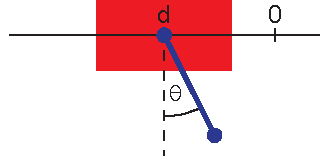
\includegraphics[width=0.5\textwidth]{images/ddpg/pendulum.pdf}
\caption{Pendulum state representation}
\label{fig:pendulum}
\end{figure}

The reward was transferred to the agent as follows:

$$r_t = dt \cdot (|\phi| - 0.1\cdot |a_t| - 0.1\cdot |d|)$$

The coefficients 0.1 were picked arbitrarily, their purpose was to keep the agent from outputting too large values too often ($a_t$) and to stop the cartpole drifting too far from the center ($d$). If the episode ended before the time limit, a negative reward of -0.1 was added to the terminating state.

Video \ref{video:swingup} shows a successfully learned pendulum swingup. See \ref{tab:ddpg} for training details.

\subsubsection{Network size dependency}
During my experimentation I noticed a correlation between sizes of critic and actor networks and the convergence ability. 

When using a very small actor and a sufficiently large critic, the network was still able to learn to the extent of the actor's ability.

When using a small critic, the algorithm was unable to converge to good results. This is because the critics outputs must be accurate for the actor to learn anything. I also noticed that if the critic was too small to learn, the critic's output slowly diverged to extremely high values. This is a good indicator for checking if the critic is too small.

See \ref{plot:act-off} for comparisons.

\begin{figure}[htbp]
%% Creator: Matplotlib, PGF backend
%%
%% To include the figure in your LaTeX document, write
%%   \input{<filename>.pgf}
%%
%% Make sure the required packages are loaded in your preamble
%%   \usepackage{pgf}
%%
%% Figures using additional raster images can only be included by \input if
%% they are in the same directory as the main LaTeX file. For loading figures
%% from other directories you can use the `import` package
%%   \usepackage{import}
%% and then include the figures with
%%   \import{<path to file>}{<filename>.pgf}
%%
%% Matplotlib used the following preamble
%%   \usepackage[utf8x]{inputenc}
%%   \usepackage[T1]{fontenc}
%%
\begingroup%
\makeatletter%
\begin{pgfpicture}%
\pgfpathrectangle{\pgfpointorigin}{\pgfqpoint{5.022831in}{2.009132in}}%
\pgfusepath{use as bounding box, clip}%
\begin{pgfscope}%
\pgfsetbuttcap%
\pgfsetmiterjoin%
\definecolor{currentfill}{rgb}{1.000000,1.000000,1.000000}%
\pgfsetfillcolor{currentfill}%
\pgfsetlinewidth{0.000000pt}%
\definecolor{currentstroke}{rgb}{1.000000,1.000000,1.000000}%
\pgfsetstrokecolor{currentstroke}%
\pgfsetdash{}{0pt}%
\pgfpathmoveto{\pgfqpoint{0.000000in}{0.000000in}}%
\pgfpathlineto{\pgfqpoint{5.022831in}{0.000000in}}%
\pgfpathlineto{\pgfqpoint{5.022831in}{2.009132in}}%
\pgfpathlineto{\pgfqpoint{0.000000in}{2.009132in}}%
\pgfpathclose%
\pgfusepath{fill}%
\end{pgfscope}%
\begin{pgfscope}%
\pgfsetbuttcap%
\pgfsetmiterjoin%
\definecolor{currentfill}{rgb}{1.000000,1.000000,1.000000}%
\pgfsetfillcolor{currentfill}%
\pgfsetlinewidth{0.000000pt}%
\definecolor{currentstroke}{rgb}{0.000000,0.000000,0.000000}%
\pgfsetstrokecolor{currentstroke}%
\pgfsetstrokeopacity{0.000000}%
\pgfsetdash{}{0pt}%
\pgfpathmoveto{\pgfqpoint{0.397655in}{0.495779in}}%
\pgfpathlineto{\pgfqpoint{4.754774in}{0.495779in}}%
\pgfpathlineto{\pgfqpoint{4.754774in}{1.859132in}}%
\pgfpathlineto{\pgfqpoint{0.397655in}{1.859132in}}%
\pgfpathclose%
\pgfusepath{fill}%
\end{pgfscope}%
\begin{pgfscope}%
\pgfpathrectangle{\pgfqpoint{0.397655in}{0.495779in}}{\pgfqpoint{4.357119in}{1.363353in}} %
\pgfusepath{clip}%
\pgfsetrectcap%
\pgfsetroundjoin%
\pgfsetlinewidth{0.501875pt}%
\definecolor{currentstroke}{rgb}{0.000000,0.000000,1.000000}%
\pgfsetstrokecolor{currentstroke}%
\pgfsetdash{}{0pt}%
\pgfpathmoveto{\pgfqpoint{0.397446in}{0.679360in}}%
\pgfpathlineto{\pgfqpoint{0.406784in}{0.691633in}}%
\pgfpathlineto{\pgfqpoint{0.431323in}{0.691532in}}%
\pgfpathlineto{\pgfqpoint{0.434956in}{0.716836in}}%
\pgfpathlineto{\pgfqpoint{0.440527in}{0.816995in}}%
\pgfpathlineto{\pgfqpoint{0.447776in}{0.804223in}}%
\pgfpathlineto{\pgfqpoint{0.454699in}{0.808928in}}%
\pgfpathlineto{\pgfqpoint{0.462210in}{0.818756in}}%
\pgfpathlineto{\pgfqpoint{0.468652in}{0.822685in}}%
\pgfpathlineto{\pgfqpoint{0.489554in}{0.828280in}}%
\pgfpathlineto{\pgfqpoint{0.497546in}{0.824787in}}%
\pgfpathlineto{\pgfqpoint{0.505391in}{0.830524in}}%
\pgfpathlineto{\pgfqpoint{0.518790in}{0.837159in}}%
\pgfpathlineto{\pgfqpoint{0.525622in}{0.845316in}}%
\pgfpathlineto{\pgfqpoint{0.532830in}{0.831803in}}%
\pgfpathlineto{\pgfqpoint{0.539974in}{0.832384in}}%
\pgfpathlineto{\pgfqpoint{0.547024in}{0.810017in}}%
\pgfpathlineto{\pgfqpoint{0.554691in}{0.805341in}}%
\pgfpathlineto{\pgfqpoint{0.561406in}{0.809027in}}%
\pgfpathlineto{\pgfqpoint{0.568942in}{0.816182in}}%
\pgfpathlineto{\pgfqpoint{0.576635in}{0.810474in}}%
\pgfpathlineto{\pgfqpoint{0.584657in}{0.812516in}}%
\pgfpathlineto{\pgfqpoint{0.592429in}{0.810255in}}%
\pgfpathlineto{\pgfqpoint{0.600927in}{0.823887in}}%
\pgfpathlineto{\pgfqpoint{0.610401in}{0.819623in}}%
\pgfpathlineto{\pgfqpoint{0.634832in}{1.036346in}}%
\pgfpathlineto{\pgfqpoint{0.665083in}{1.256785in}}%
\pgfpathlineto{\pgfqpoint{0.696438in}{1.222233in}}%
\pgfpathlineto{\pgfqpoint{0.727794in}{1.277544in}}%
\pgfpathlineto{\pgfqpoint{0.759150in}{1.246033in}}%
\pgfpathlineto{\pgfqpoint{0.788307in}{1.261698in}}%
\pgfpathlineto{\pgfqpoint{0.819663in}{1.331505in}}%
\pgfpathlineto{\pgfqpoint{0.851019in}{1.222999in}}%
\pgfpathlineto{\pgfqpoint{0.882374in}{1.311450in}}%
\pgfpathlineto{\pgfqpoint{0.913730in}{1.282091in}}%
\pgfpathlineto{\pgfqpoint{0.976441in}{1.337121in}}%
\pgfpathlineto{\pgfqpoint{1.000403in}{0.850529in}}%
\pgfpathlineto{\pgfqpoint{1.024930in}{1.071714in}}%
\pgfpathlineto{\pgfqpoint{1.056286in}{1.270787in}}%
\pgfpathlineto{\pgfqpoint{1.087641in}{1.344528in}}%
\pgfpathlineto{\pgfqpoint{1.117990in}{1.241853in}}%
\pgfpathlineto{\pgfqpoint{1.149345in}{1.265507in}}%
\pgfpathlineto{\pgfqpoint{1.180701in}{1.302976in}}%
\pgfpathlineto{\pgfqpoint{1.212056in}{1.305816in}}%
\pgfpathlineto{\pgfqpoint{1.243412in}{1.269876in}}%
\pgfpathlineto{\pgfqpoint{1.274768in}{1.324563in}}%
\pgfpathlineto{\pgfqpoint{1.306123in}{1.331569in}}%
\pgfpathlineto{\pgfqpoint{1.337479in}{1.325877in}}%
\pgfpathlineto{\pgfqpoint{1.368834in}{1.348868in}}%
\pgfpathlineto{\pgfqpoint{1.400190in}{1.336387in}}%
\pgfpathlineto{\pgfqpoint{1.429360in}{1.339435in}}%
\pgfpathlineto{\pgfqpoint{1.458866in}{1.345629in}}%
\pgfpathlineto{\pgfqpoint{1.490222in}{1.406959in}}%
\pgfpathlineto{\pgfqpoint{1.521577in}{1.379669in}}%
\pgfpathlineto{\pgfqpoint{1.552933in}{1.400137in}}%
\pgfpathlineto{\pgfqpoint{1.584289in}{1.395239in}}%
\pgfpathlineto{\pgfqpoint{1.615644in}{1.350554in}}%
\pgfpathlineto{\pgfqpoint{1.647000in}{1.423242in}}%
\pgfpathlineto{\pgfqpoint{1.678355in}{1.400044in}}%
\pgfpathlineto{\pgfqpoint{1.709711in}{1.344463in}}%
\pgfpathlineto{\pgfqpoint{1.741066in}{1.413012in}}%
\pgfpathlineto{\pgfqpoint{1.772422in}{1.400370in}}%
\pgfpathlineto{\pgfqpoint{1.803778in}{1.402064in}}%
\pgfpathlineto{\pgfqpoint{1.866489in}{1.222110in}}%
\pgfpathlineto{\pgfqpoint{1.897844in}{1.377399in}}%
\pgfpathlineto{\pgfqpoint{1.929200in}{1.407818in}}%
\pgfpathlineto{\pgfqpoint{1.960555in}{1.435845in}}%
\pgfpathlineto{\pgfqpoint{1.991911in}{1.332787in}}%
\pgfpathlineto{\pgfqpoint{2.020295in}{1.397191in}}%
\pgfpathlineto{\pgfqpoint{2.051651in}{1.401518in}}%
\pgfpathlineto{\pgfqpoint{2.083006in}{1.337623in}}%
\pgfpathlineto{\pgfqpoint{2.114362in}{1.325651in}}%
\pgfpathlineto{\pgfqpoint{2.145717in}{1.387430in}}%
\pgfpathlineto{\pgfqpoint{2.177073in}{1.372985in}}%
\pgfpathlineto{\pgfqpoint{2.208428in}{1.398878in}}%
\pgfpathlineto{\pgfqpoint{2.239784in}{1.387616in}}%
\pgfpathlineto{\pgfqpoint{2.271139in}{1.403938in}}%
\pgfpathlineto{\pgfqpoint{2.302495in}{1.375673in}}%
\pgfpathlineto{\pgfqpoint{2.330766in}{1.391344in}}%
\pgfpathlineto{\pgfqpoint{2.362121in}{1.358294in}}%
\pgfpathlineto{\pgfqpoint{2.393477in}{1.426132in}}%
\pgfpathlineto{\pgfqpoint{2.424832in}{1.425057in}}%
\pgfpathlineto{\pgfqpoint{2.456188in}{1.416368in}}%
\pgfpathlineto{\pgfqpoint{2.487544in}{1.415062in}}%
\pgfpathlineto{\pgfqpoint{2.518899in}{1.421698in}}%
\pgfpathlineto{\pgfqpoint{2.550255in}{1.413705in}}%
\pgfpathlineto{\pgfqpoint{2.581610in}{1.377704in}}%
\pgfpathlineto{\pgfqpoint{2.612966in}{1.358755in}}%
\pgfpathlineto{\pgfqpoint{2.644321in}{1.292851in}}%
\pgfpathlineto{\pgfqpoint{2.673450in}{1.290092in}}%
\pgfpathlineto{\pgfqpoint{2.704805in}{1.332464in}}%
\pgfpathlineto{\pgfqpoint{2.736161in}{1.365099in}}%
\pgfpathlineto{\pgfqpoint{2.767516in}{1.343556in}}%
\pgfpathlineto{\pgfqpoint{2.797138in}{1.366577in}}%
\pgfpathlineto{\pgfqpoint{2.828493in}{1.440504in}}%
\pgfpathlineto{\pgfqpoint{2.859849in}{1.418843in}}%
\pgfpathlineto{\pgfqpoint{2.891205in}{1.430195in}}%
\pgfpathlineto{\pgfqpoint{2.922560in}{1.393444in}}%
\pgfpathlineto{\pgfqpoint{2.953916in}{1.351502in}}%
\pgfpathlineto{\pgfqpoint{3.016627in}{1.376491in}}%
\pgfpathlineto{\pgfqpoint{3.047177in}{1.454203in}}%
\pgfpathlineto{\pgfqpoint{3.076135in}{1.340746in}}%
\pgfpathlineto{\pgfqpoint{3.101146in}{1.660199in}}%
\pgfpathlineto{\pgfqpoint{3.129511in}{1.610956in}}%
\pgfpathlineto{\pgfqpoint{3.156781in}{1.397482in}}%
\pgfpathlineto{\pgfqpoint{3.181249in}{1.470456in}}%
\pgfpathlineto{\pgfqpoint{3.210970in}{1.649904in}}%
\pgfpathlineto{\pgfqpoint{3.228747in}{0.757658in}}%
\pgfpathlineto{\pgfqpoint{3.248274in}{1.432420in}}%
\pgfpathlineto{\pgfqpoint{3.272850in}{1.630964in}}%
\pgfpathlineto{\pgfqpoint{3.304205in}{1.383934in}}%
\pgfpathlineto{\pgfqpoint{3.335561in}{1.545946in}}%
\pgfpathlineto{\pgfqpoint{3.366916in}{1.287713in}}%
\pgfpathlineto{\pgfqpoint{3.398272in}{1.507206in}}%
\pgfpathlineto{\pgfqpoint{3.417457in}{1.452399in}}%
\pgfpathlineto{\pgfqpoint{3.445418in}{1.616680in}}%
\pgfpathlineto{\pgfqpoint{3.475168in}{1.580825in}}%
\pgfpathlineto{\pgfqpoint{3.504964in}{1.679358in}}%
\pgfpathlineto{\pgfqpoint{3.535190in}{1.582444in}}%
\pgfpathlineto{\pgfqpoint{3.564575in}{1.527273in}}%
\pgfpathlineto{\pgfqpoint{3.592049in}{1.565688in}}%
\pgfpathlineto{\pgfqpoint{3.614664in}{0.990215in}}%
\pgfpathlineto{\pgfqpoint{3.643320in}{0.967722in}}%
\pgfpathlineto{\pgfqpoint{3.662819in}{1.031240in}}%
\pgfpathlineto{\pgfqpoint{3.689146in}{1.413502in}}%
\pgfpathlineto{\pgfqpoint{3.713260in}{1.071963in}}%
\pgfpathlineto{\pgfqpoint{3.740712in}{1.689596in}}%
\pgfpathlineto{\pgfqpoint{3.765853in}{1.280009in}}%
\pgfpathlineto{\pgfqpoint{3.791488in}{1.546587in}}%
\pgfpathlineto{\pgfqpoint{3.818650in}{1.426722in}}%
\pgfpathlineto{\pgfqpoint{3.841105in}{1.398666in}}%
\pgfpathlineto{\pgfqpoint{3.865976in}{1.433631in}}%
\pgfpathlineto{\pgfqpoint{3.882855in}{1.093743in}}%
\pgfpathlineto{\pgfqpoint{3.906234in}{1.412473in}}%
\pgfpathlineto{\pgfqpoint{3.919744in}{1.259081in}}%
\pgfpathlineto{\pgfqpoint{3.946633in}{1.304740in}}%
\pgfpathlineto{\pgfqpoint{3.973147in}{1.652271in}}%
\pgfpathlineto{\pgfqpoint{3.991372in}{1.343325in}}%
\pgfpathlineto{\pgfqpoint{4.017682in}{1.288359in}}%
\pgfpathlineto{\pgfqpoint{4.041925in}{1.462658in}}%
\pgfpathlineto{\pgfqpoint{4.062703in}{1.187786in}}%
\pgfpathlineto{\pgfqpoint{4.086042in}{1.035353in}}%
\pgfpathlineto{\pgfqpoint{4.112163in}{1.623356in}}%
\pgfpathlineto{\pgfqpoint{4.136846in}{1.736069in}}%
\pgfpathlineto{\pgfqpoint{4.162436in}{1.743661in}}%
\pgfpathlineto{\pgfqpoint{4.171600in}{1.334829in}}%
\pgfpathlineto{\pgfqpoint{4.195660in}{1.453768in}}%
\pgfpathlineto{\pgfqpoint{4.221893in}{1.042028in}}%
\pgfpathlineto{\pgfqpoint{4.242844in}{1.613057in}}%
\pgfpathlineto{\pgfqpoint{4.267495in}{1.451803in}}%
\pgfpathlineto{\pgfqpoint{4.287302in}{1.660142in}}%
\pgfpathlineto{\pgfqpoint{4.303145in}{0.915094in}}%
\pgfpathlineto{\pgfqpoint{4.317723in}{0.996328in}}%
\pgfpathlineto{\pgfqpoint{4.333827in}{0.969761in}}%
\pgfpathlineto{\pgfqpoint{4.355857in}{1.257650in}}%
\pgfpathlineto{\pgfqpoint{4.373728in}{1.460287in}}%
\pgfpathlineto{\pgfqpoint{4.392396in}{1.313069in}}%
\pgfpathlineto{\pgfqpoint{4.414800in}{1.571431in}}%
\pgfpathlineto{\pgfqpoint{4.434540in}{1.568008in}}%
\pgfpathlineto{\pgfqpoint{4.453101in}{1.750115in}}%
\pgfpathlineto{\pgfqpoint{4.476007in}{1.700719in}}%
\pgfpathlineto{\pgfqpoint{4.491255in}{0.980531in}}%
\pgfpathlineto{\pgfqpoint{4.507715in}{1.755812in}}%
\pgfpathlineto{\pgfqpoint{4.523824in}{1.153907in}}%
\pgfpathlineto{\pgfqpoint{4.536587in}{1.551954in}}%
\pgfpathlineto{\pgfqpoint{4.554066in}{0.947272in}}%
\pgfpathlineto{\pgfqpoint{4.566954in}{0.970059in}}%
\pgfpathlineto{\pgfqpoint{4.588492in}{0.947372in}}%
\pgfpathlineto{\pgfqpoint{4.602696in}{1.121486in}}%
\pgfpathlineto{\pgfqpoint{4.619508in}{1.027449in}}%
\pgfpathlineto{\pgfqpoint{4.635488in}{1.070447in}}%
\pgfpathlineto{\pgfqpoint{4.649150in}{1.685743in}}%
\pgfpathlineto{\pgfqpoint{4.665444in}{1.077328in}}%
\pgfpathlineto{\pgfqpoint{4.679553in}{1.196682in}}%
\pgfpathlineto{\pgfqpoint{4.694475in}{1.172530in}}%
\pgfpathlineto{\pgfqpoint{4.713517in}{1.662247in}}%
\pgfpathlineto{\pgfqpoint{4.732788in}{1.213451in}}%
\pgfpathlineto{\pgfqpoint{4.748646in}{0.970900in}}%
\pgfpathlineto{\pgfqpoint{4.764774in}{1.080375in}}%
\pgfpathlineto{\pgfqpoint{4.764774in}{1.080375in}}%
\pgfusepath{stroke}%
\end{pgfscope}%
\begin{pgfscope}%
\pgfpathrectangle{\pgfqpoint{0.397655in}{0.495779in}}{\pgfqpoint{4.357119in}{1.363353in}} %
\pgfusepath{clip}%
\pgfsetrectcap%
\pgfsetroundjoin%
\pgfsetlinewidth{0.501875pt}%
\definecolor{currentstroke}{rgb}{0.000000,0.500000,0.000000}%
\pgfsetstrokecolor{currentstroke}%
\pgfsetdash{}{0pt}%
\pgfpathmoveto{\pgfqpoint{0.396719in}{0.687056in}}%
\pgfpathlineto{\pgfqpoint{0.400926in}{0.691770in}}%
\pgfpathlineto{\pgfqpoint{0.424042in}{0.691615in}}%
\pgfpathlineto{\pgfqpoint{4.758085in}{0.691615in}}%
\pgfpathlineto{\pgfqpoint{4.758085in}{0.691615in}}%
\pgfusepath{stroke}%
\end{pgfscope}%
\begin{pgfscope}%
\pgfpathrectangle{\pgfqpoint{0.397655in}{0.495779in}}{\pgfqpoint{4.357119in}{1.363353in}} %
\pgfusepath{clip}%
\pgfsetrectcap%
\pgfsetroundjoin%
\pgfsetlinewidth{0.501875pt}%
\definecolor{currentstroke}{rgb}{1.000000,0.000000,0.000000}%
\pgfsetstrokecolor{currentstroke}%
\pgfsetdash{}{0pt}%
\pgfpathmoveto{\pgfqpoint{0.390232in}{0.681638in}}%
\pgfpathlineto{\pgfqpoint{0.405442in}{0.877286in}}%
\pgfpathlineto{\pgfqpoint{0.418202in}{0.822808in}}%
\pgfpathlineto{\pgfqpoint{0.428223in}{0.803586in}}%
\pgfpathlineto{\pgfqpoint{0.437152in}{0.814636in}}%
\pgfpathlineto{\pgfqpoint{0.446110in}{0.812387in}}%
\pgfpathlineto{\pgfqpoint{0.463435in}{0.813854in}}%
\pgfpathlineto{\pgfqpoint{0.471043in}{0.815002in}}%
\pgfpathlineto{\pgfqpoint{0.487213in}{0.822459in}}%
\pgfpathlineto{\pgfqpoint{0.495472in}{0.822646in}}%
\pgfpathlineto{\pgfqpoint{0.505166in}{0.825475in}}%
\pgfpathlineto{\pgfqpoint{0.514611in}{0.826623in}}%
\pgfpathlineto{\pgfqpoint{0.523107in}{0.829474in}}%
\pgfpathlineto{\pgfqpoint{0.532285in}{0.834992in}}%
\pgfpathlineto{\pgfqpoint{0.543411in}{0.836367in}}%
\pgfpathlineto{\pgfqpoint{0.558466in}{0.955617in}}%
\pgfpathlineto{\pgfqpoint{0.575708in}{1.065818in}}%
\pgfpathlineto{\pgfqpoint{0.599008in}{1.145598in}}%
\pgfpathlineto{\pgfqpoint{0.630364in}{1.219886in}}%
\pgfpathlineto{\pgfqpoint{0.661719in}{1.257547in}}%
\pgfpathlineto{\pgfqpoint{0.693075in}{1.300258in}}%
\pgfpathlineto{\pgfqpoint{0.724430in}{1.292452in}}%
\pgfpathlineto{\pgfqpoint{0.755786in}{1.283017in}}%
\pgfpathlineto{\pgfqpoint{0.787141in}{1.280018in}}%
\pgfpathlineto{\pgfqpoint{0.817913in}{1.260917in}}%
\pgfpathlineto{\pgfqpoint{0.849269in}{1.268084in}}%
\pgfpathlineto{\pgfqpoint{0.880624in}{1.261771in}}%
\pgfpathlineto{\pgfqpoint{0.911980in}{1.291678in}}%
\pgfpathlineto{\pgfqpoint{0.943335in}{1.277492in}}%
\pgfpathlineto{\pgfqpoint{0.974691in}{1.274870in}}%
\pgfpathlineto{\pgfqpoint{1.006047in}{1.254934in}}%
\pgfpathlineto{\pgfqpoint{1.037402in}{1.276606in}}%
\pgfpathlineto{\pgfqpoint{1.068758in}{1.259796in}}%
\pgfpathlineto{\pgfqpoint{1.100113in}{1.284829in}}%
\pgfpathlineto{\pgfqpoint{1.131469in}{1.278322in}}%
\pgfpathlineto{\pgfqpoint{1.162824in}{1.281236in}}%
\pgfpathlineto{\pgfqpoint{1.194180in}{1.285824in}}%
\pgfpathlineto{\pgfqpoint{1.225536in}{1.273156in}}%
\pgfpathlineto{\pgfqpoint{1.256891in}{1.274511in}}%
\pgfpathlineto{\pgfqpoint{1.288247in}{1.266011in}}%
\pgfpathlineto{\pgfqpoint{1.319602in}{1.286994in}}%
\pgfpathlineto{\pgfqpoint{1.350958in}{1.292341in}}%
\pgfpathlineto{\pgfqpoint{1.382313in}{1.256998in}}%
\pgfpathlineto{\pgfqpoint{1.413669in}{1.292116in}}%
\pgfpathlineto{\pgfqpoint{1.444202in}{1.275938in}}%
\pgfpathlineto{\pgfqpoint{1.475558in}{1.264284in}}%
\pgfpathlineto{\pgfqpoint{1.506913in}{1.279766in}}%
\pgfpathlineto{\pgfqpoint{1.538269in}{1.275921in}}%
\pgfpathlineto{\pgfqpoint{1.569624in}{1.269195in}}%
\pgfpathlineto{\pgfqpoint{1.598845in}{1.271170in}}%
\pgfpathlineto{\pgfqpoint{1.630200in}{1.284495in}}%
\pgfpathlineto{\pgfqpoint{1.661556in}{1.286366in}}%
\pgfpathlineto{\pgfqpoint{1.692911in}{1.285659in}}%
\pgfpathlineto{\pgfqpoint{1.724267in}{1.318917in}}%
\pgfpathlineto{\pgfqpoint{1.755623in}{1.288637in}}%
\pgfpathlineto{\pgfqpoint{1.786978in}{1.280918in}}%
\pgfpathlineto{\pgfqpoint{1.818334in}{1.266425in}}%
\pgfpathlineto{\pgfqpoint{1.849689in}{1.280311in}}%
\pgfpathlineto{\pgfqpoint{1.881045in}{1.268123in}}%
\pgfpathlineto{\pgfqpoint{1.912400in}{1.292556in}}%
\pgfpathlineto{\pgfqpoint{1.943756in}{1.281846in}}%
\pgfpathlineto{\pgfqpoint{1.975112in}{1.280757in}}%
\pgfpathlineto{\pgfqpoint{2.006467in}{1.266579in}}%
\pgfpathlineto{\pgfqpoint{2.037823in}{1.274850in}}%
\pgfpathlineto{\pgfqpoint{2.069178in}{1.275892in}}%
\pgfpathlineto{\pgfqpoint{2.100534in}{1.321643in}}%
\pgfpathlineto{\pgfqpoint{2.131889in}{1.302560in}}%
\pgfpathlineto{\pgfqpoint{2.163245in}{1.306110in}}%
\pgfpathlineto{\pgfqpoint{2.194601in}{1.297194in}}%
\pgfpathlineto{\pgfqpoint{2.257312in}{1.268669in}}%
\pgfpathlineto{\pgfqpoint{2.288667in}{1.262009in}}%
\pgfpathlineto{\pgfqpoint{2.320023in}{1.279119in}}%
\pgfpathlineto{\pgfqpoint{2.382734in}{1.285221in}}%
\pgfpathlineto{\pgfqpoint{2.414090in}{1.264634in}}%
\pgfpathlineto{\pgfqpoint{2.445445in}{1.279664in}}%
\pgfpathlineto{\pgfqpoint{2.476801in}{1.287329in}}%
\pgfpathlineto{\pgfqpoint{2.508156in}{1.271845in}}%
\pgfpathlineto{\pgfqpoint{2.539512in}{1.267285in}}%
\pgfpathlineto{\pgfqpoint{2.570867in}{1.266182in}}%
\pgfpathlineto{\pgfqpoint{2.602223in}{1.259215in}}%
\pgfpathlineto{\pgfqpoint{2.633579in}{1.274055in}}%
\pgfpathlineto{\pgfqpoint{2.664934in}{1.276564in}}%
\pgfpathlineto{\pgfqpoint{2.696290in}{1.276968in}}%
\pgfpathlineto{\pgfqpoint{2.727645in}{1.289663in}}%
\pgfpathlineto{\pgfqpoint{2.759001in}{1.272159in}}%
\pgfpathlineto{\pgfqpoint{2.790356in}{1.278363in}}%
\pgfpathlineto{\pgfqpoint{2.821255in}{1.268663in}}%
\pgfpathlineto{\pgfqpoint{2.852611in}{1.295431in}}%
\pgfpathlineto{\pgfqpoint{2.882684in}{1.266249in}}%
\pgfpathlineto{\pgfqpoint{2.914039in}{1.278287in}}%
\pgfpathlineto{\pgfqpoint{2.945395in}{1.266121in}}%
\pgfpathlineto{\pgfqpoint{2.976750in}{1.273271in}}%
\pgfpathlineto{\pgfqpoint{3.008106in}{1.260908in}}%
\pgfpathlineto{\pgfqpoint{3.039462in}{1.258387in}}%
\pgfpathlineto{\pgfqpoint{3.070817in}{1.262936in}}%
\pgfpathlineto{\pgfqpoint{3.102173in}{1.265007in}}%
\pgfpathlineto{\pgfqpoint{3.133528in}{1.287681in}}%
\pgfpathlineto{\pgfqpoint{3.164361in}{1.280692in}}%
\pgfpathlineto{\pgfqpoint{3.195717in}{1.270637in}}%
\pgfpathlineto{\pgfqpoint{3.227072in}{1.283872in}}%
\pgfpathlineto{\pgfqpoint{3.257689in}{1.277017in}}%
\pgfpathlineto{\pgfqpoint{3.289044in}{1.275356in}}%
\pgfpathlineto{\pgfqpoint{3.320400in}{1.300737in}}%
\pgfpathlineto{\pgfqpoint{3.351755in}{1.265677in}}%
\pgfpathlineto{\pgfqpoint{3.382501in}{1.287710in}}%
\pgfpathlineto{\pgfqpoint{3.413857in}{1.280020in}}%
\pgfpathlineto{\pgfqpoint{3.445212in}{1.273652in}}%
\pgfpathlineto{\pgfqpoint{3.476568in}{1.275432in}}%
\pgfpathlineto{\pgfqpoint{3.507923in}{1.275377in}}%
\pgfpathlineto{\pgfqpoint{3.539279in}{1.260407in}}%
\pgfpathlineto{\pgfqpoint{3.570634in}{1.264991in}}%
\pgfpathlineto{\pgfqpoint{3.601990in}{1.267032in}}%
\pgfpathlineto{\pgfqpoint{3.633346in}{1.263003in}}%
\pgfpathlineto{\pgfqpoint{3.664701in}{1.262088in}}%
\pgfpathlineto{\pgfqpoint{3.696057in}{1.266817in}}%
\pgfpathlineto{\pgfqpoint{3.727412in}{1.264035in}}%
\pgfpathlineto{\pgfqpoint{3.758768in}{1.280692in}}%
\pgfpathlineto{\pgfqpoint{3.790123in}{1.264953in}}%
\pgfpathlineto{\pgfqpoint{3.821479in}{1.258801in}}%
\pgfpathlineto{\pgfqpoint{3.852835in}{1.257464in}}%
\pgfpathlineto{\pgfqpoint{3.884190in}{1.275552in}}%
\pgfpathlineto{\pgfqpoint{3.915546in}{1.279138in}}%
\pgfpathlineto{\pgfqpoint{3.945434in}{1.256257in}}%
\pgfpathlineto{\pgfqpoint{3.975343in}{1.269331in}}%
\pgfpathlineto{\pgfqpoint{4.006698in}{1.277622in}}%
\pgfpathlineto{\pgfqpoint{4.038054in}{1.255349in}}%
\pgfpathlineto{\pgfqpoint{4.069410in}{1.266089in}}%
\pgfpathlineto{\pgfqpoint{4.100765in}{1.280224in}}%
\pgfpathlineto{\pgfqpoint{4.132121in}{1.276680in}}%
\pgfpathlineto{\pgfqpoint{4.163476in}{1.300845in}}%
\pgfpathlineto{\pgfqpoint{4.194832in}{1.278528in}}%
\pgfpathlineto{\pgfqpoint{4.226187in}{1.275042in}}%
\pgfpathlineto{\pgfqpoint{4.257543in}{1.259608in}}%
\pgfpathlineto{\pgfqpoint{4.288898in}{1.258037in}}%
\pgfpathlineto{\pgfqpoint{4.320254in}{1.266349in}}%
\pgfpathlineto{\pgfqpoint{4.351610in}{1.265203in}}%
\pgfpathlineto{\pgfqpoint{4.382965in}{1.262851in}}%
\pgfpathlineto{\pgfqpoint{4.414321in}{1.281018in}}%
\pgfpathlineto{\pgfqpoint{4.445676in}{1.271263in}}%
\pgfpathlineto{\pgfqpoint{4.477032in}{1.259181in}}%
\pgfpathlineto{\pgfqpoint{4.508387in}{1.254051in}}%
\pgfpathlineto{\pgfqpoint{4.539743in}{1.251340in}}%
\pgfpathlineto{\pgfqpoint{4.571099in}{1.250919in}}%
\pgfpathlineto{\pgfqpoint{4.602454in}{1.290496in}}%
\pgfpathlineto{\pgfqpoint{4.633810in}{1.257512in}}%
\pgfpathlineto{\pgfqpoint{4.664745in}{1.259503in}}%
\pgfpathlineto{\pgfqpoint{4.695829in}{1.269145in}}%
\pgfpathlineto{\pgfqpoint{4.727137in}{1.251557in}}%
\pgfpathlineto{\pgfqpoint{4.756660in}{1.265853in}}%
\pgfpathlineto{\pgfqpoint{4.756660in}{1.265853in}}%
\pgfusepath{stroke}%
\end{pgfscope}%
\begin{pgfscope}%
\pgfsetrectcap%
\pgfsetmiterjoin%
\pgfsetlinewidth{1.003750pt}%
\definecolor{currentstroke}{rgb}{0.000000,0.000000,0.000000}%
\pgfsetstrokecolor{currentstroke}%
\pgfsetdash{}{0pt}%
\pgfpathmoveto{\pgfqpoint{0.397655in}{1.859132in}}%
\pgfpathlineto{\pgfqpoint{4.754774in}{1.859132in}}%
\pgfusepath{stroke}%
\end{pgfscope}%
\begin{pgfscope}%
\pgfsetrectcap%
\pgfsetmiterjoin%
\pgfsetlinewidth{1.003750pt}%
\definecolor{currentstroke}{rgb}{0.000000,0.000000,0.000000}%
\pgfsetstrokecolor{currentstroke}%
\pgfsetdash{}{0pt}%
\pgfpathmoveto{\pgfqpoint{4.754774in}{0.495779in}}%
\pgfpathlineto{\pgfqpoint{4.754774in}{1.859132in}}%
\pgfusepath{stroke}%
\end{pgfscope}%
\begin{pgfscope}%
\pgfsetrectcap%
\pgfsetmiterjoin%
\pgfsetlinewidth{1.003750pt}%
\definecolor{currentstroke}{rgb}{0.000000,0.000000,0.000000}%
\pgfsetstrokecolor{currentstroke}%
\pgfsetdash{}{0pt}%
\pgfpathmoveto{\pgfqpoint{0.397655in}{0.495779in}}%
\pgfpathlineto{\pgfqpoint{4.754774in}{0.495779in}}%
\pgfusepath{stroke}%
\end{pgfscope}%
\begin{pgfscope}%
\pgfsetrectcap%
\pgfsetmiterjoin%
\pgfsetlinewidth{1.003750pt}%
\definecolor{currentstroke}{rgb}{0.000000,0.000000,0.000000}%
\pgfsetstrokecolor{currentstroke}%
\pgfsetdash{}{0pt}%
\pgfpathmoveto{\pgfqpoint{0.397655in}{0.495779in}}%
\pgfpathlineto{\pgfqpoint{0.397655in}{1.859132in}}%
\pgfusepath{stroke}%
\end{pgfscope}%
\begin{pgfscope}%
\pgfpathrectangle{\pgfqpoint{0.397655in}{0.495779in}}{\pgfqpoint{4.357119in}{1.363353in}} %
\pgfusepath{clip}%
\pgfsetbuttcap%
\pgfsetroundjoin%
\pgfsetlinewidth{0.501875pt}%
\definecolor{currentstroke}{rgb}{0.000000,0.000000,0.000000}%
\pgfsetstrokecolor{currentstroke}%
\pgfsetdash{{1.000000pt}{3.000000pt}}{0.000000pt}%
\pgfpathmoveto{\pgfqpoint{0.397655in}{0.495779in}}%
\pgfpathlineto{\pgfqpoint{0.397655in}{1.859132in}}%
\pgfusepath{stroke}%
\end{pgfscope}%
\begin{pgfscope}%
\pgfsetbuttcap%
\pgfsetroundjoin%
\definecolor{currentfill}{rgb}{0.000000,0.000000,0.000000}%
\pgfsetfillcolor{currentfill}%
\pgfsetlinewidth{0.501875pt}%
\definecolor{currentstroke}{rgb}{0.000000,0.000000,0.000000}%
\pgfsetstrokecolor{currentstroke}%
\pgfsetdash{}{0pt}%
\pgfsys@defobject{currentmarker}{\pgfqpoint{0.000000in}{0.000000in}}{\pgfqpoint{0.000000in}{0.055556in}}{%
\pgfpathmoveto{\pgfqpoint{0.000000in}{0.000000in}}%
\pgfpathlineto{\pgfqpoint{0.000000in}{0.055556in}}%
\pgfusepath{stroke,fill}%
}%
\begin{pgfscope}%
\pgfsys@transformshift{0.397655in}{0.495779in}%
\pgfsys@useobject{currentmarker}{}%
\end{pgfscope}%
\end{pgfscope}%
\begin{pgfscope}%
\pgfsetbuttcap%
\pgfsetroundjoin%
\definecolor{currentfill}{rgb}{0.000000,0.000000,0.000000}%
\pgfsetfillcolor{currentfill}%
\pgfsetlinewidth{0.501875pt}%
\definecolor{currentstroke}{rgb}{0.000000,0.000000,0.000000}%
\pgfsetstrokecolor{currentstroke}%
\pgfsetdash{}{0pt}%
\pgfsys@defobject{currentmarker}{\pgfqpoint{0.000000in}{-0.055556in}}{\pgfqpoint{0.000000in}{0.000000in}}{%
\pgfpathmoveto{\pgfqpoint{0.000000in}{0.000000in}}%
\pgfpathlineto{\pgfqpoint{0.000000in}{-0.055556in}}%
\pgfusepath{stroke,fill}%
}%
\begin{pgfscope}%
\pgfsys@transformshift{0.397655in}{1.859132in}%
\pgfsys@useobject{currentmarker}{}%
\end{pgfscope}%
\end{pgfscope}%
\begin{pgfscope}%
\pgftext[x=0.397655in,y=0.440224in,,top]{\fontsize{8.000000}{9.600000}\selectfont \(\displaystyle 0\)}%
\end{pgfscope}%
\begin{pgfscope}%
\pgfpathrectangle{\pgfqpoint{0.397655in}{0.495779in}}{\pgfqpoint{4.357119in}{1.363353in}} %
\pgfusepath{clip}%
\pgfsetbuttcap%
\pgfsetroundjoin%
\pgfsetlinewidth{0.501875pt}%
\definecolor{currentstroke}{rgb}{0.000000,0.000000,0.000000}%
\pgfsetstrokecolor{currentstroke}%
\pgfsetdash{{1.000000pt}{3.000000pt}}{0.000000pt}%
\pgfpathmoveto{\pgfqpoint{1.269079in}{0.495779in}}%
\pgfpathlineto{\pgfqpoint{1.269079in}{1.859132in}}%
\pgfusepath{stroke}%
\end{pgfscope}%
\begin{pgfscope}%
\pgfsetbuttcap%
\pgfsetroundjoin%
\definecolor{currentfill}{rgb}{0.000000,0.000000,0.000000}%
\pgfsetfillcolor{currentfill}%
\pgfsetlinewidth{0.501875pt}%
\definecolor{currentstroke}{rgb}{0.000000,0.000000,0.000000}%
\pgfsetstrokecolor{currentstroke}%
\pgfsetdash{}{0pt}%
\pgfsys@defobject{currentmarker}{\pgfqpoint{0.000000in}{0.000000in}}{\pgfqpoint{0.000000in}{0.055556in}}{%
\pgfpathmoveto{\pgfqpoint{0.000000in}{0.000000in}}%
\pgfpathlineto{\pgfqpoint{0.000000in}{0.055556in}}%
\pgfusepath{stroke,fill}%
}%
\begin{pgfscope}%
\pgfsys@transformshift{1.269079in}{0.495779in}%
\pgfsys@useobject{currentmarker}{}%
\end{pgfscope}%
\end{pgfscope}%
\begin{pgfscope}%
\pgfsetbuttcap%
\pgfsetroundjoin%
\definecolor{currentfill}{rgb}{0.000000,0.000000,0.000000}%
\pgfsetfillcolor{currentfill}%
\pgfsetlinewidth{0.501875pt}%
\definecolor{currentstroke}{rgb}{0.000000,0.000000,0.000000}%
\pgfsetstrokecolor{currentstroke}%
\pgfsetdash{}{0pt}%
\pgfsys@defobject{currentmarker}{\pgfqpoint{0.000000in}{-0.055556in}}{\pgfqpoint{0.000000in}{0.000000in}}{%
\pgfpathmoveto{\pgfqpoint{0.000000in}{0.000000in}}%
\pgfpathlineto{\pgfqpoint{0.000000in}{-0.055556in}}%
\pgfusepath{stroke,fill}%
}%
\begin{pgfscope}%
\pgfsys@transformshift{1.269079in}{1.859132in}%
\pgfsys@useobject{currentmarker}{}%
\end{pgfscope}%
\end{pgfscope}%
\begin{pgfscope}%
\pgftext[x=1.269079in,y=0.440224in,,top]{\fontsize{8.000000}{9.600000}\selectfont \(\displaystyle 500\)}%
\end{pgfscope}%
\begin{pgfscope}%
\pgfpathrectangle{\pgfqpoint{0.397655in}{0.495779in}}{\pgfqpoint{4.357119in}{1.363353in}} %
\pgfusepath{clip}%
\pgfsetbuttcap%
\pgfsetroundjoin%
\pgfsetlinewidth{0.501875pt}%
\definecolor{currentstroke}{rgb}{0.000000,0.000000,0.000000}%
\pgfsetstrokecolor{currentstroke}%
\pgfsetdash{{1.000000pt}{3.000000pt}}{0.000000pt}%
\pgfpathmoveto{\pgfqpoint{2.140503in}{0.495779in}}%
\pgfpathlineto{\pgfqpoint{2.140503in}{1.859132in}}%
\pgfusepath{stroke}%
\end{pgfscope}%
\begin{pgfscope}%
\pgfsetbuttcap%
\pgfsetroundjoin%
\definecolor{currentfill}{rgb}{0.000000,0.000000,0.000000}%
\pgfsetfillcolor{currentfill}%
\pgfsetlinewidth{0.501875pt}%
\definecolor{currentstroke}{rgb}{0.000000,0.000000,0.000000}%
\pgfsetstrokecolor{currentstroke}%
\pgfsetdash{}{0pt}%
\pgfsys@defobject{currentmarker}{\pgfqpoint{0.000000in}{0.000000in}}{\pgfqpoint{0.000000in}{0.055556in}}{%
\pgfpathmoveto{\pgfqpoint{0.000000in}{0.000000in}}%
\pgfpathlineto{\pgfqpoint{0.000000in}{0.055556in}}%
\pgfusepath{stroke,fill}%
}%
\begin{pgfscope}%
\pgfsys@transformshift{2.140503in}{0.495779in}%
\pgfsys@useobject{currentmarker}{}%
\end{pgfscope}%
\end{pgfscope}%
\begin{pgfscope}%
\pgfsetbuttcap%
\pgfsetroundjoin%
\definecolor{currentfill}{rgb}{0.000000,0.000000,0.000000}%
\pgfsetfillcolor{currentfill}%
\pgfsetlinewidth{0.501875pt}%
\definecolor{currentstroke}{rgb}{0.000000,0.000000,0.000000}%
\pgfsetstrokecolor{currentstroke}%
\pgfsetdash{}{0pt}%
\pgfsys@defobject{currentmarker}{\pgfqpoint{0.000000in}{-0.055556in}}{\pgfqpoint{0.000000in}{0.000000in}}{%
\pgfpathmoveto{\pgfqpoint{0.000000in}{0.000000in}}%
\pgfpathlineto{\pgfqpoint{0.000000in}{-0.055556in}}%
\pgfusepath{stroke,fill}%
}%
\begin{pgfscope}%
\pgfsys@transformshift{2.140503in}{1.859132in}%
\pgfsys@useobject{currentmarker}{}%
\end{pgfscope}%
\end{pgfscope}%
\begin{pgfscope}%
\pgftext[x=2.140503in,y=0.440224in,,top]{\fontsize{8.000000}{9.600000}\selectfont \(\displaystyle 1000\)}%
\end{pgfscope}%
\begin{pgfscope}%
\pgfpathrectangle{\pgfqpoint{0.397655in}{0.495779in}}{\pgfqpoint{4.357119in}{1.363353in}} %
\pgfusepath{clip}%
\pgfsetbuttcap%
\pgfsetroundjoin%
\pgfsetlinewidth{0.501875pt}%
\definecolor{currentstroke}{rgb}{0.000000,0.000000,0.000000}%
\pgfsetstrokecolor{currentstroke}%
\pgfsetdash{{1.000000pt}{3.000000pt}}{0.000000pt}%
\pgfpathmoveto{\pgfqpoint{3.011926in}{0.495779in}}%
\pgfpathlineto{\pgfqpoint{3.011926in}{1.859132in}}%
\pgfusepath{stroke}%
\end{pgfscope}%
\begin{pgfscope}%
\pgfsetbuttcap%
\pgfsetroundjoin%
\definecolor{currentfill}{rgb}{0.000000,0.000000,0.000000}%
\pgfsetfillcolor{currentfill}%
\pgfsetlinewidth{0.501875pt}%
\definecolor{currentstroke}{rgb}{0.000000,0.000000,0.000000}%
\pgfsetstrokecolor{currentstroke}%
\pgfsetdash{}{0pt}%
\pgfsys@defobject{currentmarker}{\pgfqpoint{0.000000in}{0.000000in}}{\pgfqpoint{0.000000in}{0.055556in}}{%
\pgfpathmoveto{\pgfqpoint{0.000000in}{0.000000in}}%
\pgfpathlineto{\pgfqpoint{0.000000in}{0.055556in}}%
\pgfusepath{stroke,fill}%
}%
\begin{pgfscope}%
\pgfsys@transformshift{3.011926in}{0.495779in}%
\pgfsys@useobject{currentmarker}{}%
\end{pgfscope}%
\end{pgfscope}%
\begin{pgfscope}%
\pgfsetbuttcap%
\pgfsetroundjoin%
\definecolor{currentfill}{rgb}{0.000000,0.000000,0.000000}%
\pgfsetfillcolor{currentfill}%
\pgfsetlinewidth{0.501875pt}%
\definecolor{currentstroke}{rgb}{0.000000,0.000000,0.000000}%
\pgfsetstrokecolor{currentstroke}%
\pgfsetdash{}{0pt}%
\pgfsys@defobject{currentmarker}{\pgfqpoint{0.000000in}{-0.055556in}}{\pgfqpoint{0.000000in}{0.000000in}}{%
\pgfpathmoveto{\pgfqpoint{0.000000in}{0.000000in}}%
\pgfpathlineto{\pgfqpoint{0.000000in}{-0.055556in}}%
\pgfusepath{stroke,fill}%
}%
\begin{pgfscope}%
\pgfsys@transformshift{3.011926in}{1.859132in}%
\pgfsys@useobject{currentmarker}{}%
\end{pgfscope}%
\end{pgfscope}%
\begin{pgfscope}%
\pgftext[x=3.011926in,y=0.440224in,,top]{\fontsize{8.000000}{9.600000}\selectfont \(\displaystyle 1500\)}%
\end{pgfscope}%
\begin{pgfscope}%
\pgfpathrectangle{\pgfqpoint{0.397655in}{0.495779in}}{\pgfqpoint{4.357119in}{1.363353in}} %
\pgfusepath{clip}%
\pgfsetbuttcap%
\pgfsetroundjoin%
\pgfsetlinewidth{0.501875pt}%
\definecolor{currentstroke}{rgb}{0.000000,0.000000,0.000000}%
\pgfsetstrokecolor{currentstroke}%
\pgfsetdash{{1.000000pt}{3.000000pt}}{0.000000pt}%
\pgfpathmoveto{\pgfqpoint{3.883350in}{0.495779in}}%
\pgfpathlineto{\pgfqpoint{3.883350in}{1.859132in}}%
\pgfusepath{stroke}%
\end{pgfscope}%
\begin{pgfscope}%
\pgfsetbuttcap%
\pgfsetroundjoin%
\definecolor{currentfill}{rgb}{0.000000,0.000000,0.000000}%
\pgfsetfillcolor{currentfill}%
\pgfsetlinewidth{0.501875pt}%
\definecolor{currentstroke}{rgb}{0.000000,0.000000,0.000000}%
\pgfsetstrokecolor{currentstroke}%
\pgfsetdash{}{0pt}%
\pgfsys@defobject{currentmarker}{\pgfqpoint{0.000000in}{0.000000in}}{\pgfqpoint{0.000000in}{0.055556in}}{%
\pgfpathmoveto{\pgfqpoint{0.000000in}{0.000000in}}%
\pgfpathlineto{\pgfqpoint{0.000000in}{0.055556in}}%
\pgfusepath{stroke,fill}%
}%
\begin{pgfscope}%
\pgfsys@transformshift{3.883350in}{0.495779in}%
\pgfsys@useobject{currentmarker}{}%
\end{pgfscope}%
\end{pgfscope}%
\begin{pgfscope}%
\pgfsetbuttcap%
\pgfsetroundjoin%
\definecolor{currentfill}{rgb}{0.000000,0.000000,0.000000}%
\pgfsetfillcolor{currentfill}%
\pgfsetlinewidth{0.501875pt}%
\definecolor{currentstroke}{rgb}{0.000000,0.000000,0.000000}%
\pgfsetstrokecolor{currentstroke}%
\pgfsetdash{}{0pt}%
\pgfsys@defobject{currentmarker}{\pgfqpoint{0.000000in}{-0.055556in}}{\pgfqpoint{0.000000in}{0.000000in}}{%
\pgfpathmoveto{\pgfqpoint{0.000000in}{0.000000in}}%
\pgfpathlineto{\pgfqpoint{0.000000in}{-0.055556in}}%
\pgfusepath{stroke,fill}%
}%
\begin{pgfscope}%
\pgfsys@transformshift{3.883350in}{1.859132in}%
\pgfsys@useobject{currentmarker}{}%
\end{pgfscope}%
\end{pgfscope}%
\begin{pgfscope}%
\pgftext[x=3.883350in,y=0.440224in,,top]{\fontsize{8.000000}{9.600000}\selectfont \(\displaystyle 2000\)}%
\end{pgfscope}%
\begin{pgfscope}%
\pgfpathrectangle{\pgfqpoint{0.397655in}{0.495779in}}{\pgfqpoint{4.357119in}{1.363353in}} %
\pgfusepath{clip}%
\pgfsetbuttcap%
\pgfsetroundjoin%
\pgfsetlinewidth{0.501875pt}%
\definecolor{currentstroke}{rgb}{0.000000,0.000000,0.000000}%
\pgfsetstrokecolor{currentstroke}%
\pgfsetdash{{1.000000pt}{3.000000pt}}{0.000000pt}%
\pgfpathmoveto{\pgfqpoint{4.754774in}{0.495779in}}%
\pgfpathlineto{\pgfqpoint{4.754774in}{1.859132in}}%
\pgfusepath{stroke}%
\end{pgfscope}%
\begin{pgfscope}%
\pgfsetbuttcap%
\pgfsetroundjoin%
\definecolor{currentfill}{rgb}{0.000000,0.000000,0.000000}%
\pgfsetfillcolor{currentfill}%
\pgfsetlinewidth{0.501875pt}%
\definecolor{currentstroke}{rgb}{0.000000,0.000000,0.000000}%
\pgfsetstrokecolor{currentstroke}%
\pgfsetdash{}{0pt}%
\pgfsys@defobject{currentmarker}{\pgfqpoint{0.000000in}{0.000000in}}{\pgfqpoint{0.000000in}{0.055556in}}{%
\pgfpathmoveto{\pgfqpoint{0.000000in}{0.000000in}}%
\pgfpathlineto{\pgfqpoint{0.000000in}{0.055556in}}%
\pgfusepath{stroke,fill}%
}%
\begin{pgfscope}%
\pgfsys@transformshift{4.754774in}{0.495779in}%
\pgfsys@useobject{currentmarker}{}%
\end{pgfscope}%
\end{pgfscope}%
\begin{pgfscope}%
\pgfsetbuttcap%
\pgfsetroundjoin%
\definecolor{currentfill}{rgb}{0.000000,0.000000,0.000000}%
\pgfsetfillcolor{currentfill}%
\pgfsetlinewidth{0.501875pt}%
\definecolor{currentstroke}{rgb}{0.000000,0.000000,0.000000}%
\pgfsetstrokecolor{currentstroke}%
\pgfsetdash{}{0pt}%
\pgfsys@defobject{currentmarker}{\pgfqpoint{0.000000in}{-0.055556in}}{\pgfqpoint{0.000000in}{0.000000in}}{%
\pgfpathmoveto{\pgfqpoint{0.000000in}{0.000000in}}%
\pgfpathlineto{\pgfqpoint{0.000000in}{-0.055556in}}%
\pgfusepath{stroke,fill}%
}%
\begin{pgfscope}%
\pgfsys@transformshift{4.754774in}{1.859132in}%
\pgfsys@useobject{currentmarker}{}%
\end{pgfscope}%
\end{pgfscope}%
\begin{pgfscope}%
\pgftext[x=4.754774in,y=0.440224in,,top]{\fontsize{8.000000}{9.600000}\selectfont \(\displaystyle 2500\)}%
\end{pgfscope}%
\begin{pgfscope}%
\pgftext[x=2.576214in,y=0.272655in,,top]{\fontsize{10.000000}{12.000000}\selectfont \# 1000s learning steps}%
\end{pgfscope}%
\begin{pgfscope}%
\pgfpathrectangle{\pgfqpoint{0.397655in}{0.495779in}}{\pgfqpoint{4.357119in}{1.363353in}} %
\pgfusepath{clip}%
\pgfsetbuttcap%
\pgfsetroundjoin%
\pgfsetlinewidth{0.501875pt}%
\definecolor{currentstroke}{rgb}{0.000000,0.000000,0.000000}%
\pgfsetstrokecolor{currentstroke}%
\pgfsetdash{{1.000000pt}{3.000000pt}}{0.000000pt}%
\pgfpathmoveto{\pgfqpoint{0.397655in}{0.495779in}}%
\pgfpathlineto{\pgfqpoint{4.754774in}{0.495779in}}%
\pgfusepath{stroke}%
\end{pgfscope}%
\begin{pgfscope}%
\pgfsetbuttcap%
\pgfsetroundjoin%
\definecolor{currentfill}{rgb}{0.000000,0.000000,0.000000}%
\pgfsetfillcolor{currentfill}%
\pgfsetlinewidth{0.501875pt}%
\definecolor{currentstroke}{rgb}{0.000000,0.000000,0.000000}%
\pgfsetstrokecolor{currentstroke}%
\pgfsetdash{}{0pt}%
\pgfsys@defobject{currentmarker}{\pgfqpoint{0.000000in}{0.000000in}}{\pgfqpoint{0.055556in}{0.000000in}}{%
\pgfpathmoveto{\pgfqpoint{0.000000in}{0.000000in}}%
\pgfpathlineto{\pgfqpoint{0.055556in}{0.000000in}}%
\pgfusepath{stroke,fill}%
}%
\begin{pgfscope}%
\pgfsys@transformshift{0.397655in}{0.495779in}%
\pgfsys@useobject{currentmarker}{}%
\end{pgfscope}%
\end{pgfscope}%
\begin{pgfscope}%
\pgfsetbuttcap%
\pgfsetroundjoin%
\definecolor{currentfill}{rgb}{0.000000,0.000000,0.000000}%
\pgfsetfillcolor{currentfill}%
\pgfsetlinewidth{0.501875pt}%
\definecolor{currentstroke}{rgb}{0.000000,0.000000,0.000000}%
\pgfsetstrokecolor{currentstroke}%
\pgfsetdash{}{0pt}%
\pgfsys@defobject{currentmarker}{\pgfqpoint{-0.055556in}{0.000000in}}{\pgfqpoint{0.000000in}{0.000000in}}{%
\pgfpathmoveto{\pgfqpoint{0.000000in}{0.000000in}}%
\pgfpathlineto{\pgfqpoint{-0.055556in}{0.000000in}}%
\pgfusepath{stroke,fill}%
}%
\begin{pgfscope}%
\pgfsys@transformshift{4.754774in}{0.495779in}%
\pgfsys@useobject{currentmarker}{}%
\end{pgfscope}%
\end{pgfscope}%
\begin{pgfscope}%
\pgfpathrectangle{\pgfqpoint{0.397655in}{0.495779in}}{\pgfqpoint{4.357119in}{1.363353in}} %
\pgfusepath{clip}%
\pgfsetbuttcap%
\pgfsetroundjoin%
\pgfsetlinewidth{0.501875pt}%
\definecolor{currentstroke}{rgb}{0.000000,0.000000,0.000000}%
\pgfsetstrokecolor{currentstroke}%
\pgfsetdash{{1.000000pt}{3.000000pt}}{0.000000pt}%
\pgfpathmoveto{\pgfqpoint{0.397655in}{0.690544in}}%
\pgfpathlineto{\pgfqpoint{4.754774in}{0.690544in}}%
\pgfusepath{stroke}%
\end{pgfscope}%
\begin{pgfscope}%
\pgfsetbuttcap%
\pgfsetroundjoin%
\definecolor{currentfill}{rgb}{0.000000,0.000000,0.000000}%
\pgfsetfillcolor{currentfill}%
\pgfsetlinewidth{0.501875pt}%
\definecolor{currentstroke}{rgb}{0.000000,0.000000,0.000000}%
\pgfsetstrokecolor{currentstroke}%
\pgfsetdash{}{0pt}%
\pgfsys@defobject{currentmarker}{\pgfqpoint{0.000000in}{0.000000in}}{\pgfqpoint{0.055556in}{0.000000in}}{%
\pgfpathmoveto{\pgfqpoint{0.000000in}{0.000000in}}%
\pgfpathlineto{\pgfqpoint{0.055556in}{0.000000in}}%
\pgfusepath{stroke,fill}%
}%
\begin{pgfscope}%
\pgfsys@transformshift{0.397655in}{0.690544in}%
\pgfsys@useobject{currentmarker}{}%
\end{pgfscope}%
\end{pgfscope}%
\begin{pgfscope}%
\pgfsetbuttcap%
\pgfsetroundjoin%
\definecolor{currentfill}{rgb}{0.000000,0.000000,0.000000}%
\pgfsetfillcolor{currentfill}%
\pgfsetlinewidth{0.501875pt}%
\definecolor{currentstroke}{rgb}{0.000000,0.000000,0.000000}%
\pgfsetstrokecolor{currentstroke}%
\pgfsetdash{}{0pt}%
\pgfsys@defobject{currentmarker}{\pgfqpoint{-0.055556in}{0.000000in}}{\pgfqpoint{0.000000in}{0.000000in}}{%
\pgfpathmoveto{\pgfqpoint{0.000000in}{0.000000in}}%
\pgfpathlineto{\pgfqpoint{-0.055556in}{0.000000in}}%
\pgfusepath{stroke,fill}%
}%
\begin{pgfscope}%
\pgfsys@transformshift{4.754774in}{0.690544in}%
\pgfsys@useobject{currentmarker}{}%
\end{pgfscope}%
\end{pgfscope}%
\begin{pgfscope}%
\pgfpathrectangle{\pgfqpoint{0.397655in}{0.495779in}}{\pgfqpoint{4.357119in}{1.363353in}} %
\pgfusepath{clip}%
\pgfsetbuttcap%
\pgfsetroundjoin%
\pgfsetlinewidth{0.501875pt}%
\definecolor{currentstroke}{rgb}{0.000000,0.000000,0.000000}%
\pgfsetstrokecolor{currentstroke}%
\pgfsetdash{{1.000000pt}{3.000000pt}}{0.000000pt}%
\pgfpathmoveto{\pgfqpoint{0.397655in}{0.885309in}}%
\pgfpathlineto{\pgfqpoint{4.754774in}{0.885309in}}%
\pgfusepath{stroke}%
\end{pgfscope}%
\begin{pgfscope}%
\pgfsetbuttcap%
\pgfsetroundjoin%
\definecolor{currentfill}{rgb}{0.000000,0.000000,0.000000}%
\pgfsetfillcolor{currentfill}%
\pgfsetlinewidth{0.501875pt}%
\definecolor{currentstroke}{rgb}{0.000000,0.000000,0.000000}%
\pgfsetstrokecolor{currentstroke}%
\pgfsetdash{}{0pt}%
\pgfsys@defobject{currentmarker}{\pgfqpoint{0.000000in}{0.000000in}}{\pgfqpoint{0.055556in}{0.000000in}}{%
\pgfpathmoveto{\pgfqpoint{0.000000in}{0.000000in}}%
\pgfpathlineto{\pgfqpoint{0.055556in}{0.000000in}}%
\pgfusepath{stroke,fill}%
}%
\begin{pgfscope}%
\pgfsys@transformshift{0.397655in}{0.885309in}%
\pgfsys@useobject{currentmarker}{}%
\end{pgfscope}%
\end{pgfscope}%
\begin{pgfscope}%
\pgfsetbuttcap%
\pgfsetroundjoin%
\definecolor{currentfill}{rgb}{0.000000,0.000000,0.000000}%
\pgfsetfillcolor{currentfill}%
\pgfsetlinewidth{0.501875pt}%
\definecolor{currentstroke}{rgb}{0.000000,0.000000,0.000000}%
\pgfsetstrokecolor{currentstroke}%
\pgfsetdash{}{0pt}%
\pgfsys@defobject{currentmarker}{\pgfqpoint{-0.055556in}{0.000000in}}{\pgfqpoint{0.000000in}{0.000000in}}{%
\pgfpathmoveto{\pgfqpoint{0.000000in}{0.000000in}}%
\pgfpathlineto{\pgfqpoint{-0.055556in}{0.000000in}}%
\pgfusepath{stroke,fill}%
}%
\begin{pgfscope}%
\pgfsys@transformshift{4.754774in}{0.885309in}%
\pgfsys@useobject{currentmarker}{}%
\end{pgfscope}%
\end{pgfscope}%
\begin{pgfscope}%
\pgfpathrectangle{\pgfqpoint{0.397655in}{0.495779in}}{\pgfqpoint{4.357119in}{1.363353in}} %
\pgfusepath{clip}%
\pgfsetbuttcap%
\pgfsetroundjoin%
\pgfsetlinewidth{0.501875pt}%
\definecolor{currentstroke}{rgb}{0.000000,0.000000,0.000000}%
\pgfsetstrokecolor{currentstroke}%
\pgfsetdash{{1.000000pt}{3.000000pt}}{0.000000pt}%
\pgfpathmoveto{\pgfqpoint{0.397655in}{1.080074in}}%
\pgfpathlineto{\pgfqpoint{4.754774in}{1.080074in}}%
\pgfusepath{stroke}%
\end{pgfscope}%
\begin{pgfscope}%
\pgfsetbuttcap%
\pgfsetroundjoin%
\definecolor{currentfill}{rgb}{0.000000,0.000000,0.000000}%
\pgfsetfillcolor{currentfill}%
\pgfsetlinewidth{0.501875pt}%
\definecolor{currentstroke}{rgb}{0.000000,0.000000,0.000000}%
\pgfsetstrokecolor{currentstroke}%
\pgfsetdash{}{0pt}%
\pgfsys@defobject{currentmarker}{\pgfqpoint{0.000000in}{0.000000in}}{\pgfqpoint{0.055556in}{0.000000in}}{%
\pgfpathmoveto{\pgfqpoint{0.000000in}{0.000000in}}%
\pgfpathlineto{\pgfqpoint{0.055556in}{0.000000in}}%
\pgfusepath{stroke,fill}%
}%
\begin{pgfscope}%
\pgfsys@transformshift{0.397655in}{1.080074in}%
\pgfsys@useobject{currentmarker}{}%
\end{pgfscope}%
\end{pgfscope}%
\begin{pgfscope}%
\pgfsetbuttcap%
\pgfsetroundjoin%
\definecolor{currentfill}{rgb}{0.000000,0.000000,0.000000}%
\pgfsetfillcolor{currentfill}%
\pgfsetlinewidth{0.501875pt}%
\definecolor{currentstroke}{rgb}{0.000000,0.000000,0.000000}%
\pgfsetstrokecolor{currentstroke}%
\pgfsetdash{}{0pt}%
\pgfsys@defobject{currentmarker}{\pgfqpoint{-0.055556in}{0.000000in}}{\pgfqpoint{0.000000in}{0.000000in}}{%
\pgfpathmoveto{\pgfqpoint{0.000000in}{0.000000in}}%
\pgfpathlineto{\pgfqpoint{-0.055556in}{0.000000in}}%
\pgfusepath{stroke,fill}%
}%
\begin{pgfscope}%
\pgfsys@transformshift{4.754774in}{1.080074in}%
\pgfsys@useobject{currentmarker}{}%
\end{pgfscope}%
\end{pgfscope}%
\begin{pgfscope}%
\pgfpathrectangle{\pgfqpoint{0.397655in}{0.495779in}}{\pgfqpoint{4.357119in}{1.363353in}} %
\pgfusepath{clip}%
\pgfsetbuttcap%
\pgfsetroundjoin%
\pgfsetlinewidth{0.501875pt}%
\definecolor{currentstroke}{rgb}{0.000000,0.000000,0.000000}%
\pgfsetstrokecolor{currentstroke}%
\pgfsetdash{{1.000000pt}{3.000000pt}}{0.000000pt}%
\pgfpathmoveto{\pgfqpoint{0.397655in}{1.274838in}}%
\pgfpathlineto{\pgfqpoint{4.754774in}{1.274838in}}%
\pgfusepath{stroke}%
\end{pgfscope}%
\begin{pgfscope}%
\pgfsetbuttcap%
\pgfsetroundjoin%
\definecolor{currentfill}{rgb}{0.000000,0.000000,0.000000}%
\pgfsetfillcolor{currentfill}%
\pgfsetlinewidth{0.501875pt}%
\definecolor{currentstroke}{rgb}{0.000000,0.000000,0.000000}%
\pgfsetstrokecolor{currentstroke}%
\pgfsetdash{}{0pt}%
\pgfsys@defobject{currentmarker}{\pgfqpoint{0.000000in}{0.000000in}}{\pgfqpoint{0.055556in}{0.000000in}}{%
\pgfpathmoveto{\pgfqpoint{0.000000in}{0.000000in}}%
\pgfpathlineto{\pgfqpoint{0.055556in}{0.000000in}}%
\pgfusepath{stroke,fill}%
}%
\begin{pgfscope}%
\pgfsys@transformshift{0.397655in}{1.274838in}%
\pgfsys@useobject{currentmarker}{}%
\end{pgfscope}%
\end{pgfscope}%
\begin{pgfscope}%
\pgfsetbuttcap%
\pgfsetroundjoin%
\definecolor{currentfill}{rgb}{0.000000,0.000000,0.000000}%
\pgfsetfillcolor{currentfill}%
\pgfsetlinewidth{0.501875pt}%
\definecolor{currentstroke}{rgb}{0.000000,0.000000,0.000000}%
\pgfsetstrokecolor{currentstroke}%
\pgfsetdash{}{0pt}%
\pgfsys@defobject{currentmarker}{\pgfqpoint{-0.055556in}{0.000000in}}{\pgfqpoint{0.000000in}{0.000000in}}{%
\pgfpathmoveto{\pgfqpoint{0.000000in}{0.000000in}}%
\pgfpathlineto{\pgfqpoint{-0.055556in}{0.000000in}}%
\pgfusepath{stroke,fill}%
}%
\begin{pgfscope}%
\pgfsys@transformshift{4.754774in}{1.274838in}%
\pgfsys@useobject{currentmarker}{}%
\end{pgfscope}%
\end{pgfscope}%
\begin{pgfscope}%
\pgfpathrectangle{\pgfqpoint{0.397655in}{0.495779in}}{\pgfqpoint{4.357119in}{1.363353in}} %
\pgfusepath{clip}%
\pgfsetbuttcap%
\pgfsetroundjoin%
\pgfsetlinewidth{0.501875pt}%
\definecolor{currentstroke}{rgb}{0.000000,0.000000,0.000000}%
\pgfsetstrokecolor{currentstroke}%
\pgfsetdash{{1.000000pt}{3.000000pt}}{0.000000pt}%
\pgfpathmoveto{\pgfqpoint{0.397655in}{1.469603in}}%
\pgfpathlineto{\pgfqpoint{4.754774in}{1.469603in}}%
\pgfusepath{stroke}%
\end{pgfscope}%
\begin{pgfscope}%
\pgfsetbuttcap%
\pgfsetroundjoin%
\definecolor{currentfill}{rgb}{0.000000,0.000000,0.000000}%
\pgfsetfillcolor{currentfill}%
\pgfsetlinewidth{0.501875pt}%
\definecolor{currentstroke}{rgb}{0.000000,0.000000,0.000000}%
\pgfsetstrokecolor{currentstroke}%
\pgfsetdash{}{0pt}%
\pgfsys@defobject{currentmarker}{\pgfqpoint{0.000000in}{0.000000in}}{\pgfqpoint{0.055556in}{0.000000in}}{%
\pgfpathmoveto{\pgfqpoint{0.000000in}{0.000000in}}%
\pgfpathlineto{\pgfqpoint{0.055556in}{0.000000in}}%
\pgfusepath{stroke,fill}%
}%
\begin{pgfscope}%
\pgfsys@transformshift{0.397655in}{1.469603in}%
\pgfsys@useobject{currentmarker}{}%
\end{pgfscope}%
\end{pgfscope}%
\begin{pgfscope}%
\pgfsetbuttcap%
\pgfsetroundjoin%
\definecolor{currentfill}{rgb}{0.000000,0.000000,0.000000}%
\pgfsetfillcolor{currentfill}%
\pgfsetlinewidth{0.501875pt}%
\definecolor{currentstroke}{rgb}{0.000000,0.000000,0.000000}%
\pgfsetstrokecolor{currentstroke}%
\pgfsetdash{}{0pt}%
\pgfsys@defobject{currentmarker}{\pgfqpoint{-0.055556in}{0.000000in}}{\pgfqpoint{0.000000in}{0.000000in}}{%
\pgfpathmoveto{\pgfqpoint{0.000000in}{0.000000in}}%
\pgfpathlineto{\pgfqpoint{-0.055556in}{0.000000in}}%
\pgfusepath{stroke,fill}%
}%
\begin{pgfscope}%
\pgfsys@transformshift{4.754774in}{1.469603in}%
\pgfsys@useobject{currentmarker}{}%
\end{pgfscope}%
\end{pgfscope}%
\begin{pgfscope}%
\pgfpathrectangle{\pgfqpoint{0.397655in}{0.495779in}}{\pgfqpoint{4.357119in}{1.363353in}} %
\pgfusepath{clip}%
\pgfsetbuttcap%
\pgfsetroundjoin%
\pgfsetlinewidth{0.501875pt}%
\definecolor{currentstroke}{rgb}{0.000000,0.000000,0.000000}%
\pgfsetstrokecolor{currentstroke}%
\pgfsetdash{{1.000000pt}{3.000000pt}}{0.000000pt}%
\pgfpathmoveto{\pgfqpoint{0.397655in}{1.664368in}}%
\pgfpathlineto{\pgfqpoint{4.754774in}{1.664368in}}%
\pgfusepath{stroke}%
\end{pgfscope}%
\begin{pgfscope}%
\pgfsetbuttcap%
\pgfsetroundjoin%
\definecolor{currentfill}{rgb}{0.000000,0.000000,0.000000}%
\pgfsetfillcolor{currentfill}%
\pgfsetlinewidth{0.501875pt}%
\definecolor{currentstroke}{rgb}{0.000000,0.000000,0.000000}%
\pgfsetstrokecolor{currentstroke}%
\pgfsetdash{}{0pt}%
\pgfsys@defobject{currentmarker}{\pgfqpoint{0.000000in}{0.000000in}}{\pgfqpoint{0.055556in}{0.000000in}}{%
\pgfpathmoveto{\pgfqpoint{0.000000in}{0.000000in}}%
\pgfpathlineto{\pgfqpoint{0.055556in}{0.000000in}}%
\pgfusepath{stroke,fill}%
}%
\begin{pgfscope}%
\pgfsys@transformshift{0.397655in}{1.664368in}%
\pgfsys@useobject{currentmarker}{}%
\end{pgfscope}%
\end{pgfscope}%
\begin{pgfscope}%
\pgfsetbuttcap%
\pgfsetroundjoin%
\definecolor{currentfill}{rgb}{0.000000,0.000000,0.000000}%
\pgfsetfillcolor{currentfill}%
\pgfsetlinewidth{0.501875pt}%
\definecolor{currentstroke}{rgb}{0.000000,0.000000,0.000000}%
\pgfsetstrokecolor{currentstroke}%
\pgfsetdash{}{0pt}%
\pgfsys@defobject{currentmarker}{\pgfqpoint{-0.055556in}{0.000000in}}{\pgfqpoint{0.000000in}{0.000000in}}{%
\pgfpathmoveto{\pgfqpoint{0.000000in}{0.000000in}}%
\pgfpathlineto{\pgfqpoint{-0.055556in}{0.000000in}}%
\pgfusepath{stroke,fill}%
}%
\begin{pgfscope}%
\pgfsys@transformshift{4.754774in}{1.664368in}%
\pgfsys@useobject{currentmarker}{}%
\end{pgfscope}%
\end{pgfscope}%
\begin{pgfscope}%
\pgfpathrectangle{\pgfqpoint{0.397655in}{0.495779in}}{\pgfqpoint{4.357119in}{1.363353in}} %
\pgfusepath{clip}%
\pgfsetbuttcap%
\pgfsetroundjoin%
\pgfsetlinewidth{0.501875pt}%
\definecolor{currentstroke}{rgb}{0.000000,0.000000,0.000000}%
\pgfsetstrokecolor{currentstroke}%
\pgfsetdash{{1.000000pt}{3.000000pt}}{0.000000pt}%
\pgfpathmoveto{\pgfqpoint{0.397655in}{1.859132in}}%
\pgfpathlineto{\pgfqpoint{4.754774in}{1.859132in}}%
\pgfusepath{stroke}%
\end{pgfscope}%
\begin{pgfscope}%
\pgfsetbuttcap%
\pgfsetroundjoin%
\definecolor{currentfill}{rgb}{0.000000,0.000000,0.000000}%
\pgfsetfillcolor{currentfill}%
\pgfsetlinewidth{0.501875pt}%
\definecolor{currentstroke}{rgb}{0.000000,0.000000,0.000000}%
\pgfsetstrokecolor{currentstroke}%
\pgfsetdash{}{0pt}%
\pgfsys@defobject{currentmarker}{\pgfqpoint{0.000000in}{0.000000in}}{\pgfqpoint{0.055556in}{0.000000in}}{%
\pgfpathmoveto{\pgfqpoint{0.000000in}{0.000000in}}%
\pgfpathlineto{\pgfqpoint{0.055556in}{0.000000in}}%
\pgfusepath{stroke,fill}%
}%
\begin{pgfscope}%
\pgfsys@transformshift{0.397655in}{1.859132in}%
\pgfsys@useobject{currentmarker}{}%
\end{pgfscope}%
\end{pgfscope}%
\begin{pgfscope}%
\pgfsetbuttcap%
\pgfsetroundjoin%
\definecolor{currentfill}{rgb}{0.000000,0.000000,0.000000}%
\pgfsetfillcolor{currentfill}%
\pgfsetlinewidth{0.501875pt}%
\definecolor{currentstroke}{rgb}{0.000000,0.000000,0.000000}%
\pgfsetstrokecolor{currentstroke}%
\pgfsetdash{}{0pt}%
\pgfsys@defobject{currentmarker}{\pgfqpoint{-0.055556in}{0.000000in}}{\pgfqpoint{0.000000in}{0.000000in}}{%
\pgfpathmoveto{\pgfqpoint{0.000000in}{0.000000in}}%
\pgfpathlineto{\pgfqpoint{-0.055556in}{0.000000in}}%
\pgfusepath{stroke,fill}%
}%
\begin{pgfscope}%
\pgfsys@transformshift{4.754774in}{1.859132in}%
\pgfsys@useobject{currentmarker}{}%
\end{pgfscope}%
\end{pgfscope}%
\begin{pgfscope}%
\pgftext[x=0.272655in,y=1.177456in,,bottom,rotate=90.000000]{\fontsize{10.000000}{12.000000}\selectfont score}%
\end{pgfscope}%
\begin{pgfscope}%
\pgfsetbuttcap%
\pgfsetmiterjoin%
\definecolor{currentfill}{rgb}{1.000000,1.000000,1.000000}%
\pgfsetfillcolor{currentfill}%
\pgfsetlinewidth{1.003750pt}%
\definecolor{currentstroke}{rgb}{0.000000,0.000000,0.000000}%
\pgfsetstrokecolor{currentstroke}%
\pgfsetdash{}{0pt}%
\pgfpathmoveto{\pgfqpoint{0.453211in}{1.615310in}}%
\pgfpathlineto{\pgfqpoint{3.789020in}{1.615310in}}%
\pgfpathlineto{\pgfqpoint{3.789020in}{1.803577in}}%
\pgfpathlineto{\pgfqpoint{0.453211in}{1.803577in}}%
\pgfpathclose%
\pgfusepath{stroke,fill}%
\end{pgfscope}%
\begin{pgfscope}%
\pgfsetrectcap%
\pgfsetroundjoin%
\pgfsetlinewidth{0.501875pt}%
\definecolor{currentstroke}{rgb}{0.000000,0.000000,1.000000}%
\pgfsetstrokecolor{currentstroke}%
\pgfsetdash{}{0pt}%
\pgfpathmoveto{\pgfqpoint{0.530988in}{1.720244in}}%
\pgfpathlineto{\pgfqpoint{0.686544in}{1.720244in}}%
\pgfusepath{stroke}%
\end{pgfscope}%
\begin{pgfscope}%
\pgftext[x=0.808766in,y=1.681355in,left,base]{\fontsize{8.000000}{9.600000}\selectfont Standard run}%
\end{pgfscope}%
\begin{pgfscope}%
\pgfsetrectcap%
\pgfsetroundjoin%
\pgfsetlinewidth{0.501875pt}%
\definecolor{currentstroke}{rgb}{0.000000,0.500000,0.000000}%
\pgfsetstrokecolor{currentstroke}%
\pgfsetdash{}{0pt}%
\pgfpathmoveto{\pgfqpoint{1.753004in}{1.720244in}}%
\pgfpathlineto{\pgfqpoint{1.908559in}{1.720244in}}%
\pgfusepath{stroke}%
\end{pgfscope}%
\begin{pgfscope}%
\pgftext[x=2.030782in,y=1.681355in,left,base]{\fontsize{8.000000}{9.600000}\selectfont Small critic}%
\end{pgfscope}%
\begin{pgfscope}%
\pgfsetrectcap%
\pgfsetroundjoin%
\pgfsetlinewidth{0.501875pt}%
\definecolor{currentstroke}{rgb}{1.000000,0.000000,0.000000}%
\pgfsetstrokecolor{currentstroke}%
\pgfsetdash{}{0pt}%
\pgfpathmoveto{\pgfqpoint{2.876567in}{1.720244in}}%
\pgfpathlineto{\pgfqpoint{3.032123in}{1.720244in}}%
\pgfusepath{stroke}%
\end{pgfscope}%
\begin{pgfscope}%
\pgftext[x=3.154345in,y=1.681355in,left,base]{\fontsize{8.000000}{9.600000}\selectfont Small actor}%
\end{pgfscope}%
\end{pgfpicture}%
\makeatother%
\endgroup%

\caption{Comparison runs on the swingup task. Actor=\{50,50\}, Critic=\{100,100\}, Small Actor=\{\}
, Small Critic=\{\}}
\centering
\label{plot:act-off}
\end{figure}

\subsection{Robot}

As previously mentioned, the robot's state representation has 27 inputs (12 positions, 12 velocities, 3 accelerometers) and 12 outputs. 

I did a few experiments using position control, however the exploration noise makes the learning harder since there is a big difference between adding a constant to the applied force (where it has the potential to start moving the joint at different speeds) and adding a constant to desired position (the consequences are much more drastic).

For this reason I used torque control in the remainder of the experiments.

\subsubsection{Maintaining balance}
The first task trained on the robot from scratch was maintaining a balance. While this task would be trivial in position control setting, when using torque control it becomes more challenging.

The reward was transferred to the agent as follows:

$$r_t = dt \cdot (1 - 0.1\cdot |a_t|)$$

If the episode ended before the time limit, a negative reward of -0.1 was added to the terminating state.

The robot was able to successfully balance after \textasciitilde 600k episodes. See video~\ref{video:standing}, \ref{tab:ddpg} for training details.

\subsubsection{Walking}
A serious problem encountered when training the robot was the training time. While 2.5 million steps of training took about 10 hours\footnote{on a 4-core 3.3 GHz CPU}, the same amount took more than 4 days on the simulator\footnote{The simulator core - physics engine, unfortunately runs on a single thread and has a significant overhead. This made training on a server unfeasible - the training process did not benefit from more CPUs and the training process of 2.5 million steps would take ~2 weeks on available server CPUs.}. I was therefore unable to conduct a full parameter search and all the mentioned tests were done on the best supervised actor \{ rnn, 10\}.

The reward was transferred to the agent as follows:

$$r_t = dt \cdot (0.1 \cdot (1.-\frac{1}{N}\sum_t|a_t|)+100\cdot\Delta x)$$

where $\Delta x$ is the change in position of the robot's torso during step $t$.

If the episode ended before the time limit, a negative reward of -0.1 was added to the terminating state.

Unfortunately due to the mentioned time requirements, I was unable to perform enough tests (or to test long enough) to prove or disprove if the algorithm is capable of walking. The best result so far was a policy that made the robot fall forward on the end of the 15 second episode time limit. It's interesting that this was possible, considering the actor has access to only a limited time frame.